%\documentclass[a4paper,twoside,openright,10pt]{memoir}
\documentclass[10pt,openright]{report}
\usepackage[utf8]{inputenc}

\synctex=1
\usepackage{xtab}


% Prepare for svenska tecken
\usepackage[T1]{fontenc}
\usepackage[swedish]{babel}
%\usepackage[]{geometry}
\addto\captionsswedish{\renewcommand{\figurename}{Bild}}
\usepackage{amsmath}
\usepackage{fancyhdr}
\usepackage{wrapfig}
\usepackage{caption}
\usepackage{framed}
\usepackage[fulladjust]{marginnote}
\usepackage{color}
\newcommand{\hilight}[1]{\colorbox{yellow}{#1}}
\usepackage{hyperref}
\hypersetup{
    colorlinks,
    citecolor=black,
    filecolor=black,
    linkcolor=black,
    urlcolor=black
}
\usepackage{stmaryrd} % För symbolen \boxbox, kräver paketet texlive-math-extra

% % % % % % % % % % % 
% Detta är nya environments för review. De bör vara relativt självförklarande hur de används.
% I princip sätter man bara den del av texten som har en viss status mellan\begin{rev-granskat} och \end{rev-granskat} tex.
% Undvik att nästla dem för det är ingen idé det fungerar inte.
% De är testade med ett antal andra environemnt som tabular mm men kolla att det fungerar med de environments du använder.
% % % % % % % % % % % % % % % % % % % % % % % % % % % % % % % % % % % % % % % % % % % % % % % % % % % % % % % % % % % % % % % 
\usepackage[svgnames,rgb]{xcolor}
\usepackage{pdfcomment}
\newenvironment{rev-ogranskat}{\begin{pdfsidelinecomment}[color=black,linewidth=3px,caption=inline]{Ogranskat}}{\end{pdfsidelinecomment}}
\newenvironment{rev-omarbetas}{\begin{pdfsidelinecomment}[color=red,linewidth=3px,caption=inline]{Omarbetas}}{\end{pdfsidelinecomment}}
\newenvironment{rev-raderas}{\begin{pdfsidelinecomment}[color=red,linewidth=3px,caption=inline]{Raderas}}{\end{pdfsidelinecomment}}
\newenvironment{rev-redo}{\begin{pdfsidelinecomment}[color=yellow,linewidth=3px,caption=inline]{Redo att granska}}{\end{pdfsidelinecomment}}
\newenvironment{rev-granskat}[1][]%
{\begin{pdfsidelinecomment}[color=green,linewidth=3px,caption=inline]%
{Granskat #1}}%
{\end{pdfsidelinecomment}}
\newenvironment{rev-nytt}[1][]%
{\begin{pdfsidelinecomment}[color=brown,linewidth=3px,caption=inline]%
{Nytt #1}}%
{\end{pdfsidelinecomment}}
\newenvironment{rev-releasat}{\begin{pdfsidelinecomment}[color=blue,linewidth=3px,caption=inline]{Klart}}{\end{pdfsidelinecomment}}

\clubpenalty=9990
\widowpenalty=9999
\brokenpenalty=4999

\usepackage[europeanvoltages,europeancurrents,europeanresistors,cuteinductors,smartlabels]{circuitikz}
\usepackage[framemethod=TikZ]{mdframed}

\mdfdefinestyle{FactBox}{%
    linecolor=blue,
    outerlinewidth=2pt,
    roundcorner=20pt,
    innertopmargin=\baselineskip,
    innerbottommargin=\baselineskip,
    innerrightmargin=20pt,
    innerleftmargin=20pt,
    backgroundcolor=gray!50!white}
\newcommand{\infobox}[1]{
\begin{wrapfigure}{r}{0.5\textwidth}
  \begin{mdframed}[style=FactBox]
#1
  \end{mdframed}
\end{wrapfigure}
}

% Prepare for tables
\usepackage{multirow}
\usepackage{longtable}

% Prepare for lists
\usepackage{enumitem}

% Prepare for graphics
\usepackage{xspace,graphicx}

\raggedbottom

% Prepare for version handling
\usepackage{xstring}
\usepackage{catchfile}
\CatchFileDef{\HEAD}{.git/refs/heads/master}{}
\newcommand{\gitrevision}{%
  \StrLeft{\HEAD}{7}%
}
\CatchFileDef{\VERSION}{VERSION.txt}{}
\newcommand{\revision}{%
  \VERSION \gitrevision%
}

%% Frontpage bacground
\usepackage{eso-pic}
\newcommand\BackgroundPic{%
\put(0,0){%
\parbox[b][\paperheight]{\paperwidth}{%
\vfill
\centering
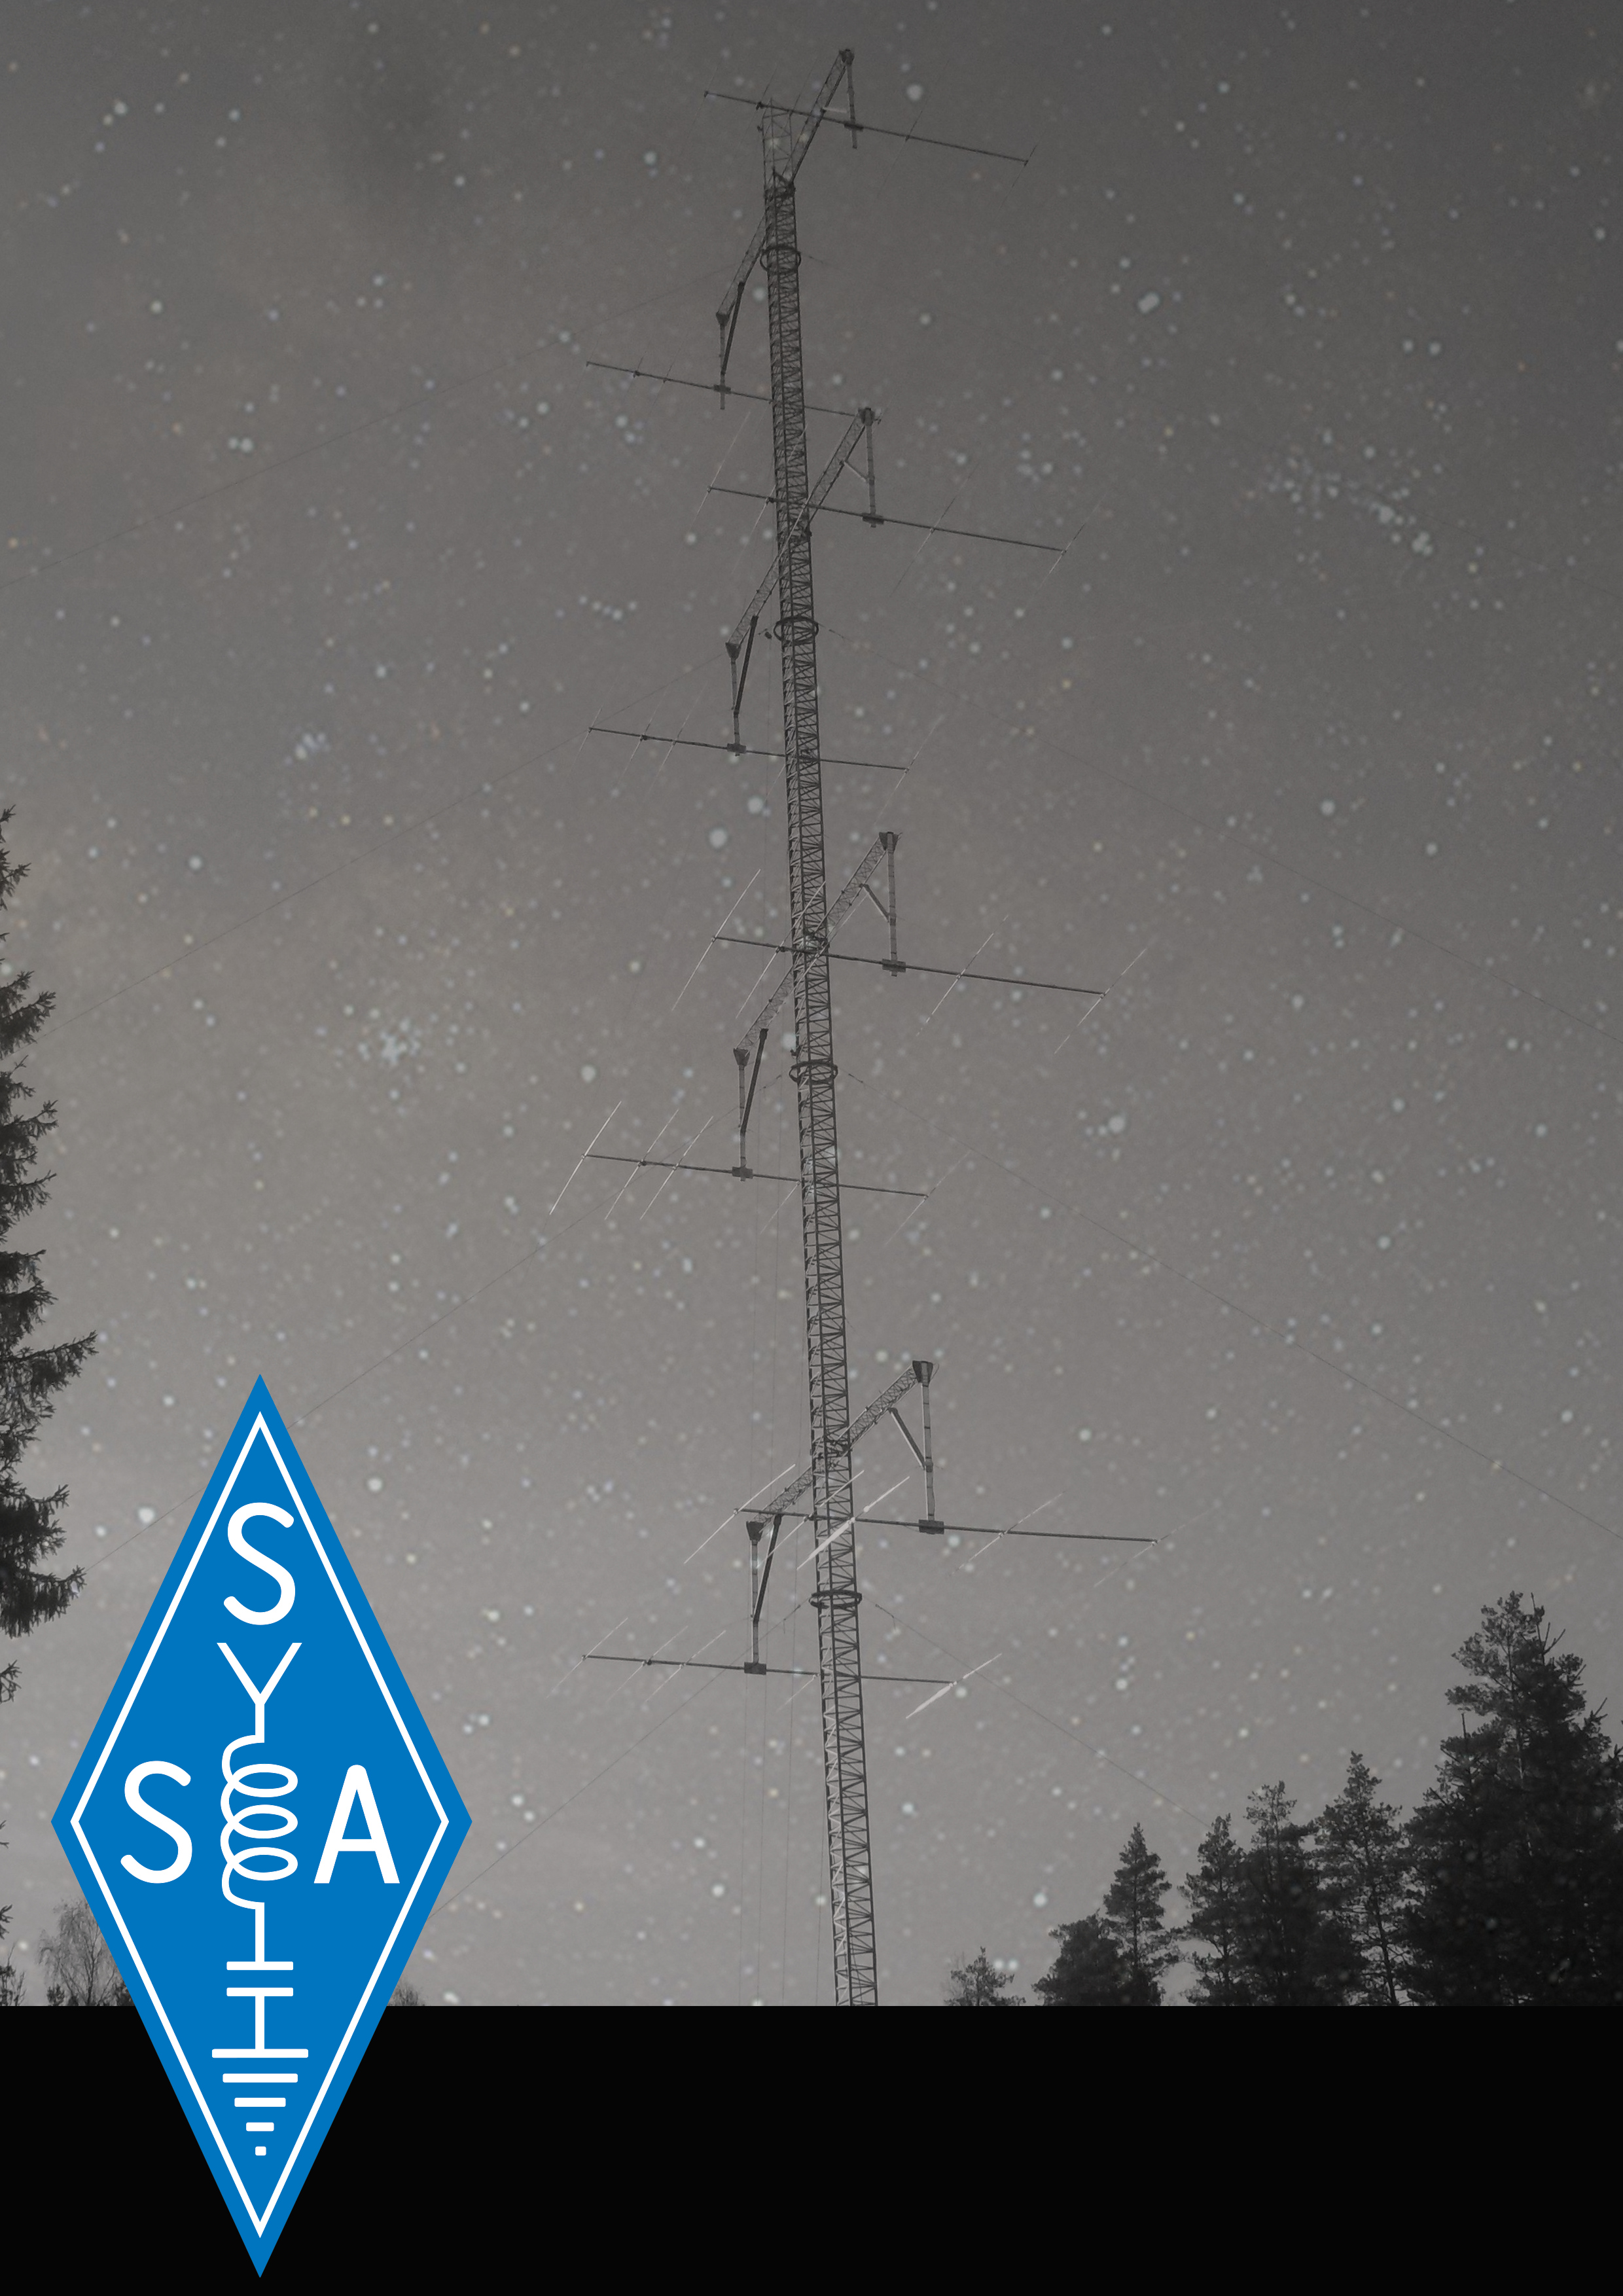
\includegraphics[width=\paperwidth,height=\paperheight,%
keepaspectratio]{images/koncept-front.jpg}%
\vfill
}}}


\newcommand\Backgroundtwo{%
\put(0,0){%
\parbox[b][\paperheight]{\paperwidth}{%
\vfill
\centering
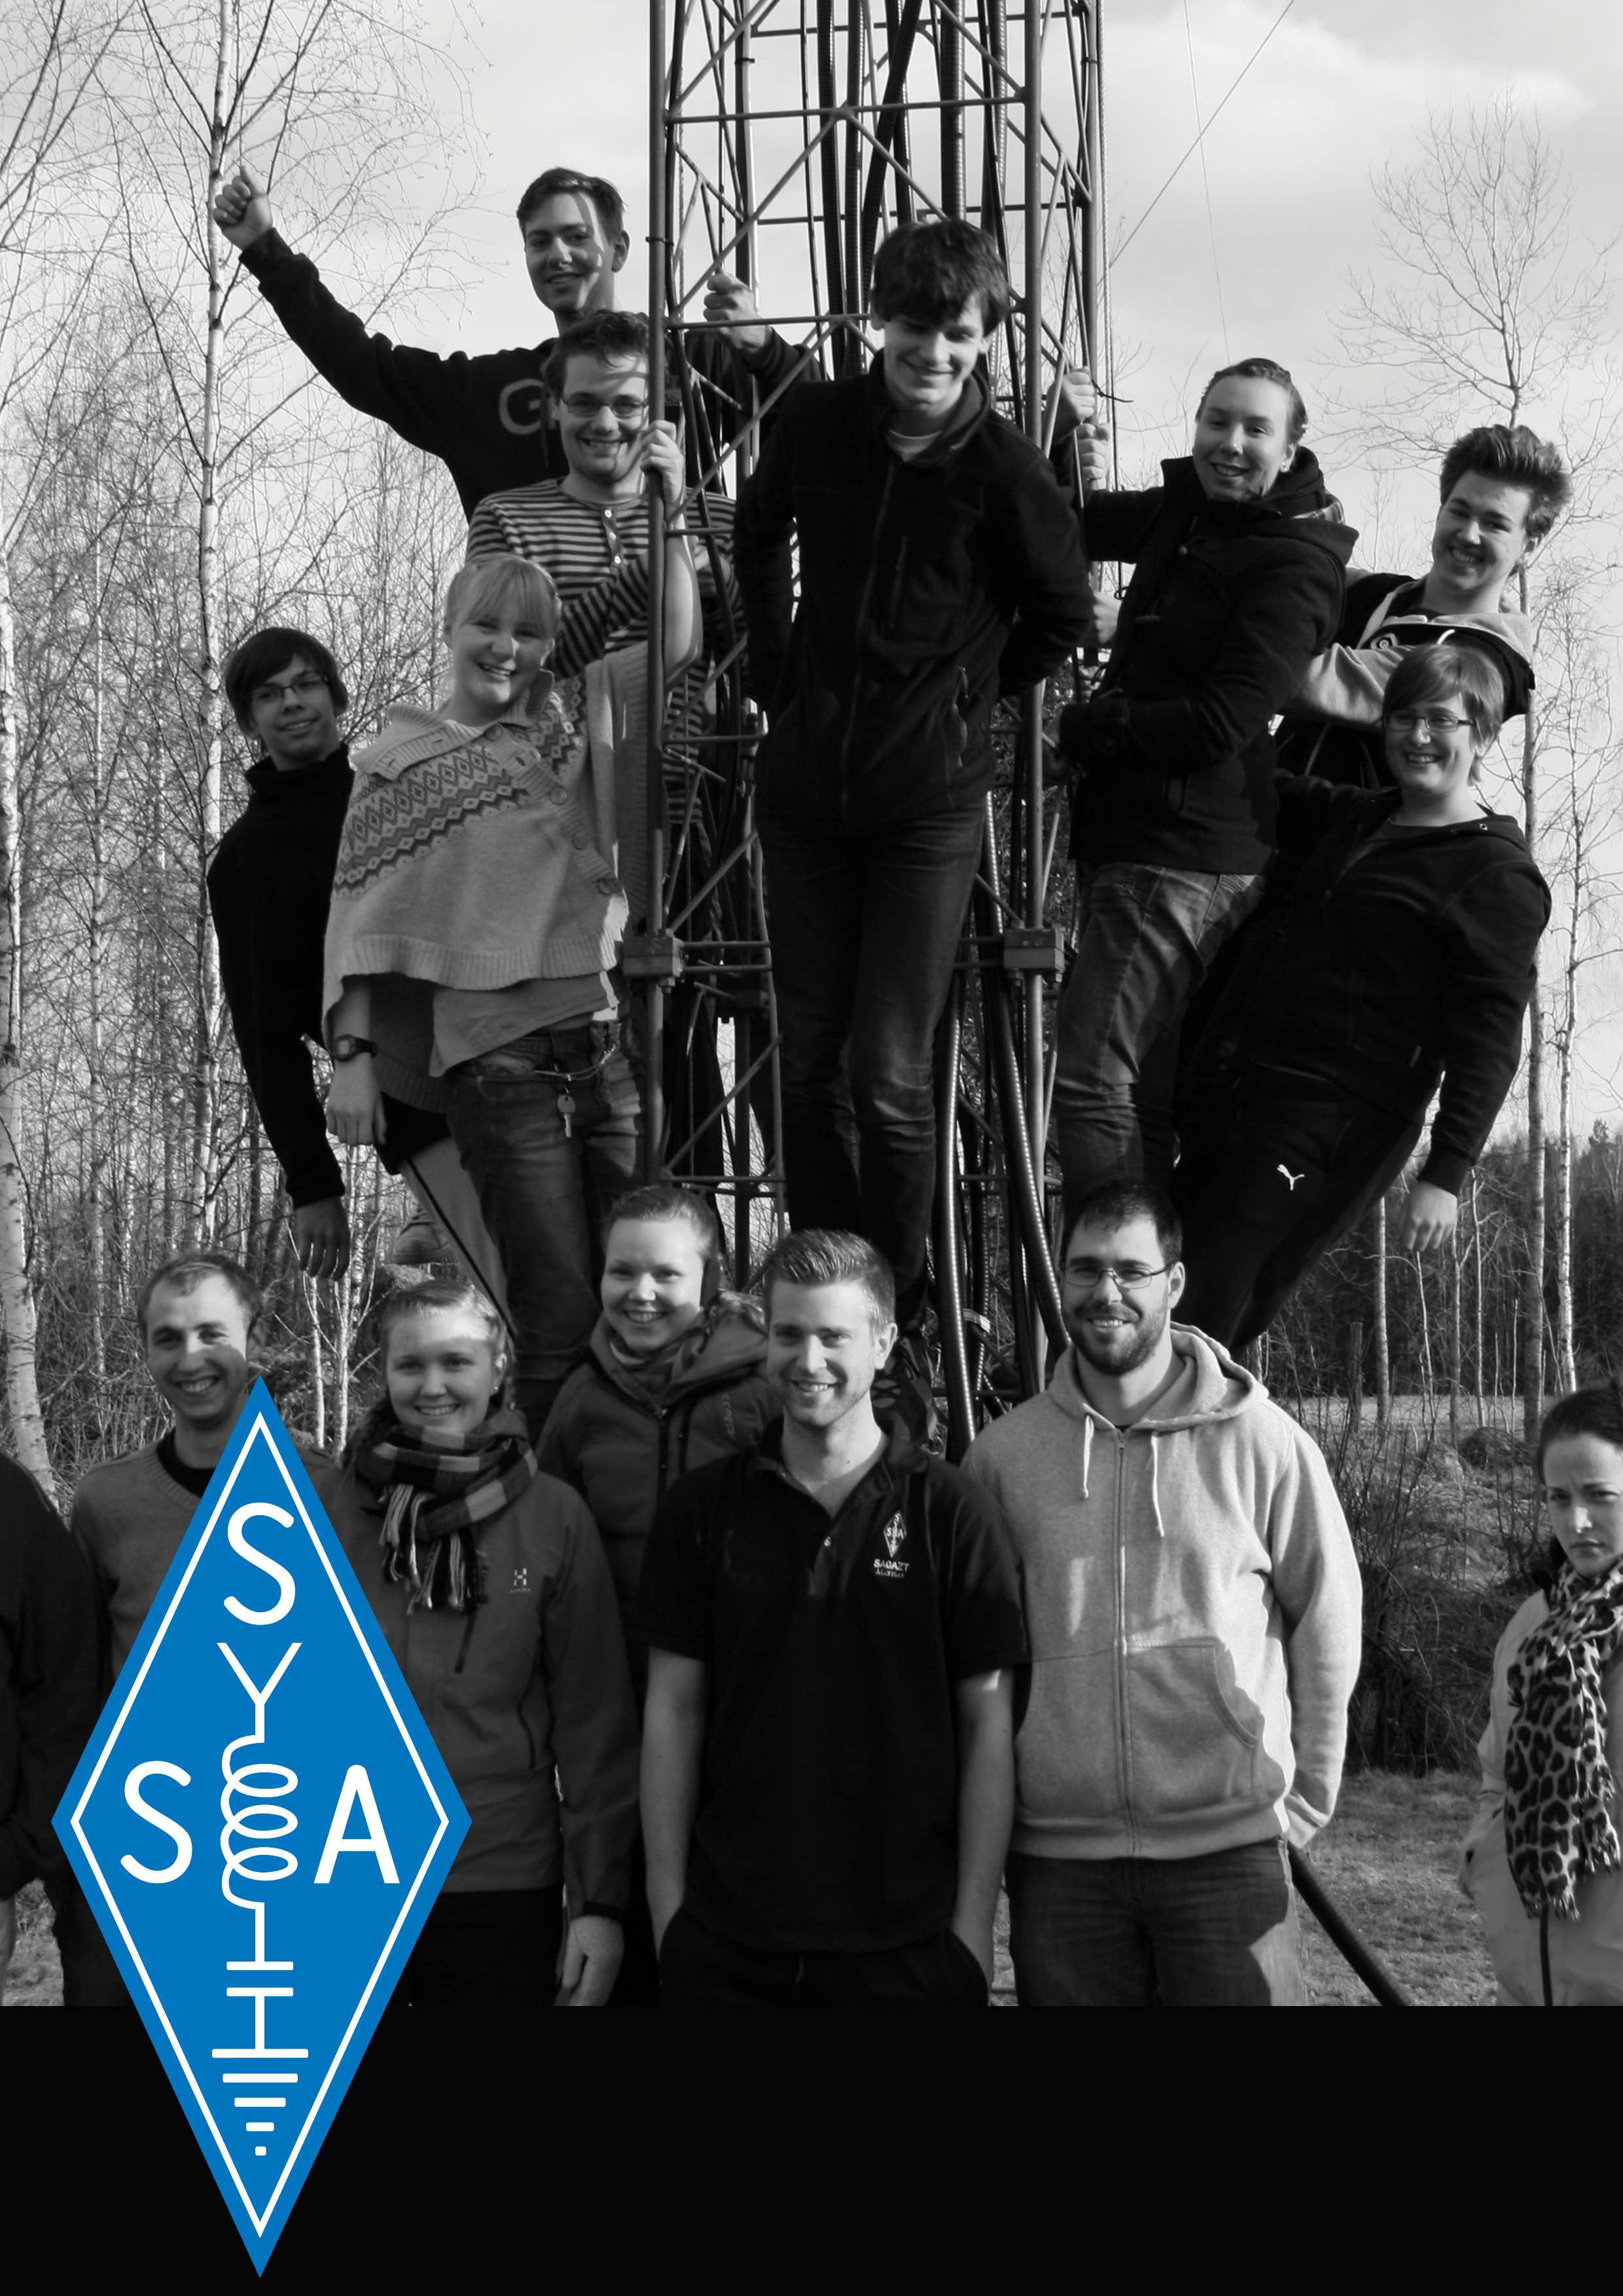
\includegraphics[width=\paperwidth,height=\paperheight,%
keepaspectratio]{images/koncept-larobok-front.jpg}%
\vfill
}}}



\newcommand\BackgroundPicLast{%
\put(0,0){%
\parbox[b][\paperheight]{\paperwidth}{%
\vfill
\centering

\includegraphics[width=\paperwidth,height=\paperheight,%
keepaspectratio]{images/koncept-back.pdf}%
\vfill
}}}

%tlfällig fix för kompilering%
%\nonstopmode
\usepackage[swedish]{babel}
% \usepackage{paralist}

\usepackage[activate={true,nocompatibility},final,tracking=true,kerning=true,spacing=true,factor=1100,stretch=10,shrink=10]{microtype}

\usepackage[a4paper,twoside,twocolumn,inner=2.2cm,outer=1.9cm,columnsep=0.9cm,top=2cm,bottom=2cm]{geometry}

\usepackage{dblfloatfix}
\usepackage{float}
\usepackage{placeins}
\usepackage{array}
\newcolumntype{L}[1]{>{\raggedright\let\newline\\\arraybackslash\hspace{0pt}}p{#1}}

\usepackage{fancyhdr}
\pagestyle{fancy}
\lhead{}
\chead{}
\rhead{}
\cfoot{}
\fancyfoot[LE,RO]{\thepage}
\renewcommand{\headrulewidth}{0pt}

\renewcommand{\bfdefault}{b}
\SetMathAlphabet{\mathbf}{normal}{OT1}{cmr}{b}{n}

\usepackage[raggedright]{titlesec}
\titlespacing{\chapter}{0pt}{1cm}{1cm}
%%\titleformat{\chapter}[hang]{\Huge\bfseries}{\thechapter\hsp\textcolor{gray75}{|}\hsp}{0pt}{\Huge\bfseries}
\titleformat{\chapter}[hang]{\Huge\bfseries}{\fcolorbox{black}{black}{\color{white}\,\vstrut\thechapter\,}~~}{0pt}{\Huge\bfseries}

%%\headheight = 12.6pt

%% \setsecnumdepth{subsection}
\setcounter{secnumdepth}{3}

% Figure macros
\newcommand{\smallfig}[4][0.4]{
  \begin{figure}[th]
    \centering
    \includegraphics[width=#1\textwidth]{#2}
    \caption{#3}
    \label{#4}
    \vspace{-10pt}
  \end{figure}
}

% Figure macros
\newcommand{\smallpagefig}[4][0.4]{
  \begin{figure*}[p]
    \centering
    \includegraphics[width=#1\textwidth]{#2}
    \caption{#3}
    \label{#4}
    \vspace{-10pt}
  \end{figure*}
}

\newcommand{\multifig}[4][0.4]{
  \begin{figure}[h]
    \centering
    \foreach \i in {#2} {
      \includegraphics[width=#1\textwidth]{\i}
    }
    \caption{#3}
    \label{#4}
    \vspace{-10pt}
  \end{figure}
}

\newcommand{\pagemultifig}[4][0.4]{
  \begin{figure}[pbt]
    \centering
    \foreach \i in {#2} {
      \includegraphics[width=#1\textwidth]{\i}
    }
    \caption{#3}
    \label{#4}
    \vspace{-10pt}
  \end{figure}
}

\newcommand{\tallfig}[4][0.4]{
  \begin{figure}
    \centering
    \includegraphics[width=#1\textwidth]{#2}
    \caption{#3}
    \label{#4}
    \vspace{-10pt}
  \end{figure}
}

\newcommand{\mediumfig}[4][0.7]{
  \begin{figure*}[bt]
    \begin{center}
      \includegraphics[width=#1\textwidth]{#2}
      \caption{#3}
      \label{#4}
    \end{center}
  \end{figure*}
}

\newcommand{\mediumtopfig}[4][0.7]{
  \begin{figure*}[t]
    \begin{center}
      \includegraphics[width=#1\textwidth]{#2}
      \caption{#3}
      \label{#4}
    \end{center}
  \end{figure*}
}

\newcommand{\pagefig}[4][0.7]{
  \begin{figure*}[pbt]
    \begin{center}
      \includegraphics[width=#1\textwidth]{#2}
      \caption{#3}
      \label{#4}
    \end{center}
  \end{figure*}
}

\newcommand{\hpfig}[4][0.6]{
  \onecolumn
  \begin{figure}[h]
    \begin{center}
      \includegraphics[width=#1\textwidth]{#2}
      \caption{#3}
      \label{#4}
    \end{center}
  \end{figure}
  \twocolumn
}

\newcommand{\largefig}[4][0.9]{
  \begin{figure*}
    \begin{center}
      \includegraphics[width=#1\textwidth]{#2}
      \caption{#3}
      \label{#4}
    \end{center}
  \end{figure*}
}

\newcommand{\smalltikz}[3]{
  \begin{figure}[h]
    \begin{center}
      #1
      \caption{#2}
      \label{#3}
    \end{center}
    \vspace{-20pt}
  \end{figure}
}

\newsavebox\TBox
\def\textoverline#1{\savebox\TBox{#1}%
  \makebox[0pt][l]{#1}\rule[1.1\ht\TBox]{\wd\TBox}{0.4pt}}

\usepackage[textfont=it,labelfont=bf,margin=10pt]{caption}

\usepackage{threeparttable}
\usepackage[symbol]{footmisc}
\usepackage{morse}
\usepackage{scalerel}
\usepackage{siunitx}

%\def\frdjp{\textbf{FÖRDJUPNING}}
\def\frdjp{}
  
% \makechapterstyle{ssa}{%
%   \chapterstyle{default}
%   \chapterstyle{article}%
%   %\renewcommand*{\thechapter}{\Roman{chapter}}
%   \renewcommand*{\printchapternum}{% center number/title
%     \centering\chapnumfont \textsc\thechapter\space\space}%
%   \renewcommand*{\printchapternonum}{\centering}
%   %\renewcommand*{\clearforchapter}{}% no new page
%   \aliaspagestyle{chapter}{headings}}% no special pagestyle

%% \semiisopage[12]

% Prepare for abstract
%\pagestyle{plain}
%\newenvironment{abstract}%
%{\cleardoubblanklepage\null \vfill\begin{center}\bfseries Abstract \end{center}}%
%{\cleardoublepage\null \vfill\begin{center}%
%\bfseries \abstractname \end{center}}%
%     {\vfill\null}

\usepackage{textbook}

% Prepare for index
\usepackage{makeidx}
\makeindex

\newcommand{\Hz}{\textit{Hz}}
\newcommand{\kHz}{\textit{kHz}}
\newcommand{\MHz}{\textit{MHz}}
\usepackage[black,sfdefault]{sourcesanspro}

\begin{document}

%% \chapterstyle{ssa}

% Frontpage
\AddToShipoutPicture*{\BackgroundPic}

\pagestyle{empty}

%\frontmatter

% Typsatt förstasida
% Här borde bilder mm in

\onecolumn
\vspace{3cm}
\begin{center}
{\fontsize{4cm}{4.8cm}\bfseries{\color{white}KonCEPT}} \\[2ex]
\Large{\bfseries{\color{white}FÖR AMATÖRRADIOCERTIFIKAT}} \\[2ex]
\huge{\color{white}Lennart Wiberg} \\
\Large{\color{white}Andra utgåvan}
\end{center}

\clearpage


% Colophone

%% Tryckortssidan
%% Tryckortssidan, denna behöver uppdateras med ny information så småningom.
\onecolumn\newgeometry{left=4cm,right=4cm}
\vspace{10em}
\title{KonCEPT för amatörradiocertifikat}
\begin{center}
\Large{KonCEPT FÖR AMATÖRRADIOCERTIFIKAT}

Föreningen Sveriges Sändareamatörer\\[2\baselineskip]
\end{center}

\noindent \textbf{Andra upplagan}

\noindent ISBN: 987-91-86368-23-4

\noindent
\\
\noindent Det här verket är licenserat under Creative Commons:\newline
\noindent Erkännande, Icke kommersiell, Dela lika\\
\noindent (CC BY-NC-SA) 4.0 Internationell.\\
\\
\\
\noindent Version \revision

\begin{figure}[h]
    
\includegraphics[width=4cm]{images/cc-by-nc-sa}
%    \caption*{CC BY-NC-SA}
\end{figure}

%Tryckt i Sverige / Printed in Sweden 1997
%Smegraf, Smedjebacken

\vfill

\noindent
\textbf{Förlag}

\noindent
\textit{Föreningen Sveriges Sändareamatörer (SSA)}\\
Box 45, SE-191 21 Sollentuna\\
Telefon +46 8 585 702 73\\
E-post \href{mailto:hq@ssa.se}{hq@ssa.se}\\[\baselineskip]
\restoregeometry\twocolumn


% \lfoot[\revision]{}
% \rfoot[]{\revision}

\cleardoublepage
%\pagestyle{fancy}

%\title{KONCEPT FÖR RADIOAMATÖRCERTIFIKAT}
%\author{Lennart Wiberg}
%\maketitle

\tableofcontents

% \setlength{\parindent}{0pt}
% \setlength{\parskip}{1ex plus 0.5ex minus 0.2ex}
 
%%\mainmatter

%\section{Rättelser}

Denna faktabok omfattar det av Post- och telestyrelsen anvisade
kompetensområdet för amatörradiocertifikat.

Innehållet är delat i två ämnesgrupper; grundläggande radioteknik
samt regler och trafikmetoder.
Det finns även inlärningsanvisningar för morsesignalering för den
som vill lära sig telegrafi.

I bilagorna finns bland annat grundläggande matematik
och frekvensplaner för amatörradiotrafik.

\chapter*{Förord}
\section*{Amatörradio}
Amatörradio är en teknisk hobby med inriktning på kommunikation och experiment
med radioanläggningar samt radiovågors utbredning. Det är en verksamhet som
utövas över hela världen av licensierade radioamatörer, även kallade
sändaramatörer.

Syftet med amatörradio är att främja personlig utveckling och internationell
förståelse samt teknisk färdighet och erfarenhetsutbyte inom området.
Amatörradio kan därtill vara en tillgång då samhällets normala resurser för
radiokommunikation behöver förstärkas.

\section*{En hobby med krav}

För att inneha och använda en radioläggning i ett land, krävs tillstånd (licens)
från dess teleadministration. För ett amatörradiotillstånd föreskrivs 
i det internationella radioreglementet bland annat handhavandemässiga och 
tekniska kvalifikationer hos varje person som önskar använda en 
amatörradiostation. De nationella teleadministrationerna tillser detta genom 
kompetensprov.

\section*{Utbildningsställen}

Amatörradioklubbarna bedriver huvuddelen av utbildningen med
amatörradiocertifikat som mål. Även vissa skolor, militära förband m.fl. har
amatörradio på programmet. I någon utsträckning förekommer även självstudier.
Rekrytering av handledare för terminslånga kurser är en nyckelfråga för
kursarrangören, liksom målinriktade, anpassade läromedel.

Tanken med denna bok är att leverera ett material som kan vara grunden till 
denna utbildning samt även för viss fördjupning och förståelse för de koncept 
som man vanligtvis stöter på inom hobbyn.

\section*{Andra förutsättningar}

Den svenska teleadministrationen har omdanats på senare tid. Därvid har även
amatörradioanvändningen berörts, främst genom att provförrättningarna för
amatörradiocertifikat delegerats till av myndigheten utsedda, ideellt arbetande
förrättare. Vidare genom att teleadministrationerna inom CEPT har infört
harmoniserade certifikats- och tillståndsklasser för amatörradio. Främst av
dessa anledningar har det uppstått behov av samordnade hjälpmedel för utbildning
och examinering, vilket amatörradiorörelsen själv har att tillgodose.

\section*{Föreningen Sveriges Sändareamatörer -- SSA}

SSA är en ideell förening för personer med intresse för amatörradio.
Verksamheten är religiöst och politiskt obunden. Ett av syftena är att bland
medlemmarna verka för ökade tekniska kunskaper och god radiotrafikkultur för att
därigenom skapa en kår av kunniga radioamatörer. SSA representerar Sverige som
nationell förening i The International Amateur Radio Union (IARU), Region 1.

\section*{Internationell samverkan}

De nationella föreningarna inom IARU samarbetar över nationsgränserna. Ett
exempel är när DARC (Deutscher Amateur-Radio-Club e.V.) för några år sedan
ställde sina Ausbildungsunterlagen till SSA:s förfogande som källmaterial för
boken El-lära och Radioteknik. Detta material har till stor del kunnat utnyttjas
även i här föreliggande bok.


\clearpage

Förord andra upplagan:

Under 2016 kom en grupp att sammankallas i en vilja att modernisera
utbildningen av radioamatörer. Denna grupp består av SSA:s utbildningsansvariga
Jonas Hulten SM5PHU, samt Magnus Danielson SA0MAD, Hans Insulander SM0UTY,
Petter Karkea SA2PKA samt Peter Lundberg SA2BLV. Utöver denna kärngrupp har
ett antal andra bidragit i stort och smått.

Dels fanns ett uppdämt behov att adressera brister i existerande
utbildningsmaterial, dels för att anpassa det till ett modernare sätt att
utbilda, vilket inkluderar att kunna nyttja moderna webbaserade
utbildningssystem. En sådan pedagogik är koncepted ''flipped classroom''
där man istället för att ha föreläsningar snarare läser hemmavid innan
lektionen och sedan försöker reda ut oklarheter och försöker
illustrera det under lektionstid. Sådan utbildningspedagogik har använts länge
t.ex. i dykutbildning hos PADI dykcenter.

En aspekt har varit att viktig är att se till att uppdatera materialet för
att täcka hela CEPT HAREC, som uppdaterats att inkludera bland annat sampling
och DSPer, vilket nu mer är en naturlig del av hobbyn. Även andra delar av
materialet har varit i behov av uppdatering.

Arbetet med att omvandla KonCEPT till \LaTeX, som bygger på den scannade och
OCR:ade versionen på första upplagan, inleddes av Magnus Danielson SA0MAD och
Hans Insulander SM0UTY. Arbetet har understötts av Thorbiörn Fritzon SA0LAT och
Täpp-Anders Sikvall SM0UEI som bidragit med sin ovärderliga \LaTeX kunskap och
SA0LAT har även gjort det stora jobbet att extrahera alla bilder från den
scannade boken och göra dem tillgängliga så att de kan läggas in.

Elsäkerhetsavsnittet has fått en ordentlig genomgång av Lorentz Björklund SM7NTJ
som även granskat igenom den övriga texten och lämnat konstruktiva synpunkter.
Regler och regelverk mm har granskats av Christer Jonson SA0BFC.

Magnus Danielson SA0MAD har skrivit nya avsnitt för digital modulation, DSP,
isolation och jordning mm. för att komplettera de hål i HAREC och materialet
som varit uppenbara.

Under arbetet har det varit viktigt att hålla spårbarhet till HAREC-krav,
vilket resulterat till Appendix L. Sakregister är också helt omarbetad för
att vara till hjälp.

\emph{Magnus Danielson SA0MAD}

\hilight{TODO: Uppdatera förord med utvecklingen.}

Förord första upplagan:

TACK!

Ett stort tack till alla dem, som på olika sätt bidragit till att förverkliga
boken. Ett särskilt tack till Bengt Falkenberg SM7EQL och Bertil Nordahl SM7CZL,
vilka har varit rådgivare och sakgranskare. Tack också till Ulf Sjöden SM6CVE
för svenska texter för bilderna från Ausbildungsunterlagen.

\emph{Författaren}


\chapter*{INLEDNING}

\Huge{VAD, HUR, VAR?}\normalsize

\section*{VAD behöver en radioamatör kunna?}

CEPT är ett samarbetsorgan mellan europeiska länders teleadministrationer
(myndigheter). En av dem är svenska Post- och telestyrelsen -- PTS.

Dessa administrationer har antagit rekommendationer om sinsemellan
harmoniserade krav på radioamatörers kompetens.

Sverige har antagit CEPT-rekommendationen T/R 61-02 \cite{TR6102}.
Vid genomförandet av kompetensprov ska de i den rekommendationen
angivna kraven särskilt beaktas.

För den som godkänts i ett sådant prov utfärdas ett harmoniserat
amatörradiocertifikat (HAREC).
Rekommendationen anger kompetensnivån HAREC.
Den svenska certifikatet bygger på CEPT HAREC krav \cite{TR6102},
med anpassning till svensk bandplan i Bilaga \ref{bandplaner}.
De detaljerade CEPT HAREC kraven finns i Bilaga \ref{CEPT HAREC}, där även
referenser till den eller de del-kapitel som avses uppfylla utbildningenkraven.

\subsection*{HUR blir man radioamatör?}

För att få sända med amatörradiosändare måste man ha amatörradiocertifikat.
Man kan antingen söka sig till någon av de klubbar som har kurs, eller skaffa
SSAs utbildningspaket och studera på egen hand. Post- och telestyrelsen har
dessutom övningsprov online som man kan testa sina kunskaper på.
När man är mogen för att avlägga certifikatprov så skriver man för någon av de
provförrättare som finns. De klubbar som har utbildning brukar planera prov
med den grupp elever de har.

Efter avlagt och godkänt prov kan man sedan ansöka om signal och certifikat,
något som SSA sköter enligt delegation från Post- och telestyrelsen.

Till tillståndet knyts en internationellt unik anropssignal. Man har möjlighet
att föreslå signal, men i brist på förslag så tas en ledig signal ur serien.

\subsection*{VAR hålls det certifikatskurser?}

Vissa amatörradioklubbar, militära förband, FRO-förbund och andra
sammanslutningar håller certifikatskurser.
Det går också att studera på egen hand.

\subsection*{VILKA läromedel behöver man?}

Denna bok omfattar hela teorin för CEPT HAREC och PTS krav.
Den ingår i det utbildningspaket som kan köpas från SSA.



\chapter{Ellära}
\label{ellära}
\chapter{Ellära}
\label{ellära}

\section{Elektriska grundbegrepp}

\harec{a}{1.1}

Elektrisk laddning, spänning och ström hänger samman med hur materian är
uppbyggd.
Den förmåga ett material har att leda laddningar, dvs. ström, kallas
konduktivitet.

\subsection{Grundämnen}
\textbf{FÖRDJUPNING}
\index{grundämnen}

Det finns många former av materia.
Ofta är en form av materia sammansatt av andra former med enklare uppbyggnad.

Sammansatt materia kan sönderdelas på kemisk väg, men däremot inte de enklaste
formerna.
All materia är uppbyggd av atomer.
De enklaste materieformerna, som kallas \emph{grundämnen}, innehåller endast
ett slags atomer.
Över 100~grundämnen är kända.

Vart och ett av grundämnena har sin speciella atomuppbyggnad och därmed en
materialstruktur, som skiljer sig från varje annat grundämne.

Tre fjärdedelar av alla grundämnen är metaller (elektriska ledare) medan de
flesta övriga är icke-metaller (isolatorer).
Det finns även en liten mellangrupp som kallas för halvledare.

\subsection{Atomernas uppbyggnad}
\textbf{FÖRDJUPNING}

Länge ansågs atomerna vara de minsta beståndsdelarna i materian.
Men omkring förra sekelskiftet upptäcktes att atomerna i sin tur består av ännu mindre
beståndsdelar, s.k. elementarpartiklar såsom protoner, neutroner, elektroner
m.fl.
Det gemensamma namnet för alla dessa partiklar är \emph{nukleoner}.

En atom består dels av en kärna som är sammansatt av protoner och neutroner,
dels av elektroner, som kretsar omkring kärnan.

\begin{quote}
\emph{Protonerna är positivt (+) laddade.}

\emph{Neutronerna är neutrala, ej laddade.}

\emph{Elektronerna är negativt (-) laddade}
\end{quote}

\begin{wrapfigure}{L}{0.5\textwidth}
  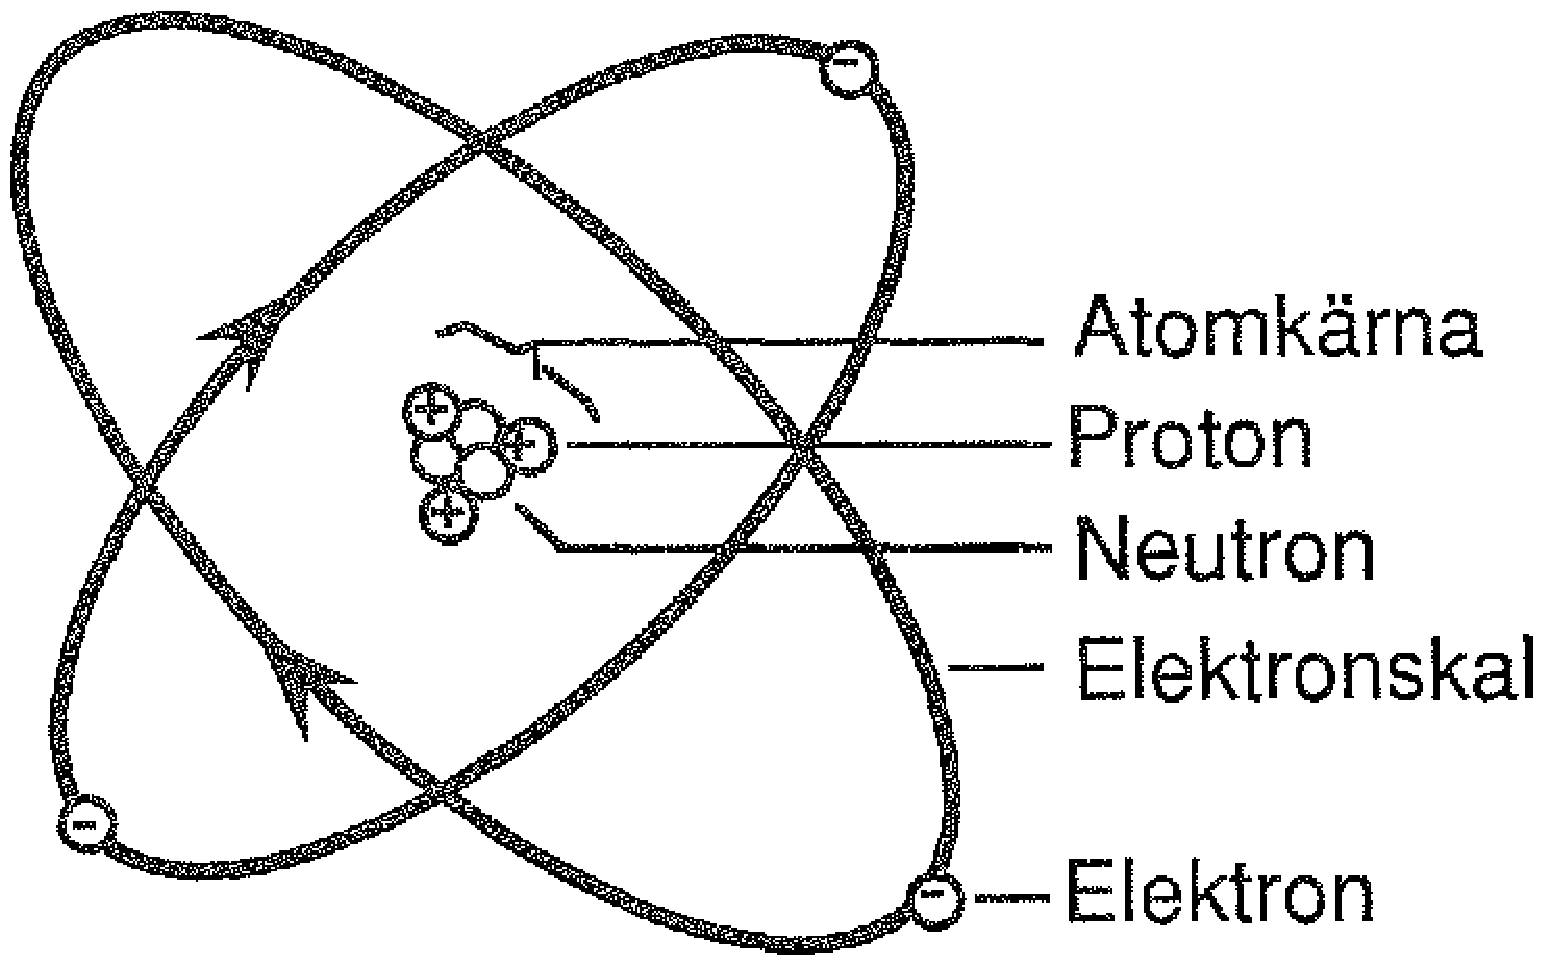
\includegraphics[width=0.5\textwidth]{images/cropped_pdfs/bild_2_1-01.pdf}
  \caption{Atomernas uppbyggnad}
  \label{fig:BildII1-1}
  \vspace{-20pt}
\end{wrapfigure}

Elektronerna kretsar i banor omkring atomkärnorna, liksom
planeterna kretsar i banor omkring sina solar, vilket illustreras i bild
\ref{fig:BildII1-1}.

Banor med samma avstånd till atomkärnan är på samma energinivå och sägs bilda
ett elektronskal.

Det kan finnas flera elektronskal.
Ju fler elektroner som finns i ett elektronskal, desto starkare är elektronerna
i skalet bundna till atomen.
Det yttersta skalet kan emellertid aldrig innehålla fler än 8~elektroner.

Elektronerna i det yttersta skalet kallas för \emph{valenselektroner}, vilka
används även av angränsande atomer vid den kemiska bindningen till
atomstrukturer, molekyler och ämnen.
För bindningen behövs ett visst antal valenselektroner.

De valenselektroner som ej behövs för bindningen kan röra sig fritt genom
materia/strukturen.
De kallas fria elektroner och är vad vi kallar elektrisk ström.

Valenselektronerna är alltså inte bara av betydelse för materialets kemiska
struktur utan också för dess elektriska egenskaper.

Atomernas massa och volym är ytterst liten.
Tag som exempel en kub av koppar med volymen \(1\ cm^3\) och vikten
\(8,9\ gram\).
Den består av ca \(8,5 \cdot 10^{22}\) kopparatomer, dvs.
\(85\, 000\, 000\, 000\, 000\, 000\, 000\, 000\) stycken.
Fenomenet metallbindning gör att antalet fria elektroner i kuben är ungefär lika
med antalet atomer i den.

Varje elementarpartikel har en massa och en atoms totala massa är summan av
elementarpartiklarnas massor.
Den enklaste atomen är väteatomen med en proton och en elektron.
Väteatomens totala massa har kunnat beräknas till \(1,66 \cdot 10^{-24}\) gram.

Nästan hela massan i atomen är samlad till kärnans protoner och neutroner.
Var och en av dem har en massa som är ungefär 2000 gånger större än massan i en
elektron.

\subsection{Elektrisk laddning och kraftverkan}
\textbf{FÖRDJUPNING}
\index{elektrisk laddning}

Enligt sägnen upptäckte Thales från Milteus redan för 2500~år sedan, att en bit
bärnsten drog till sig små grässtrån, sedan stenen gnidits mot en bit ylle.
Det grekiska ordet för bärnsten är ELEKTRON och de krafter som uppstod kom att
kallas ''elektriska''.
Av den elektriska spänningen mellan kroppar med olika laddning, verkar krafter
mellan dem och deras omgivning.
Krafterna kallas för elektriska fält och är det som gör att elektriskt laddade
kroppar kan komma i rörelse.

Ett exempel får man varje gång man kammar sig med en kam av isolerande material.
Då kommer håret att dras mot kammen därför att håret och kammen har
fått olika slags elektriska laddningar.
Samtidigt har hårstråna sinsemellan samma slags laddning och stöter bort
varandra -- håret ''reser sig''.

Lika laddningar stöter bort varandra.

Olika laddningar drar varandra till sig.

\subsection{Konduktivitet -- Ledare, halvledare och isolator}
\textbf{HAREC a.\ref{HAREC.a.1.1.1}\label{myHAREC.a.1.1.1}}
\index{konduktivitet}

En elektrisk ström sägs flyta, när de fria laddningsbärarna i ett material -- en
strömledare -- fås att röra sig samtidigt i samma riktning.
Hur många som rör sig beror på strömledarens egenskaper och spänningen mellan
ledarens ändar.

Alla material har någon grad av elektrisk ledningsförmåga som beror på
materialets atomstruktur, dimensioner och temperatur.
Vissa material (t.ex. metaller, kol, halvledare) leder elektrisk ström bättre
än andra (t.ex. glas, gummi, plast).
Mängden av fria laddningsbärare i materialet begränsar hur stor strömmen kan
bli.

\subsubsection{Ledare}
\index{ledare}
\index{konduktivitet!ledare}

Metaller har god elektrisk ledningsförmåga och kallas ledare.
Bäst ledande är de metaller, vars atomer har det minsta antalet
valenselektroner i det yttersta elektronskalet.
Koppar-, silver- och guldatomerna har en enda valenselektron och därmed mycket
god ledningsförmåga.
Järn, zink och magnesium har två valenselektroner och därmed något sämre
ledningsförmåga.
Ännu sämre ledare är de s.k. halvledarna med 3 till 5 valenselektroner.

\subsubsection{Isolatorer}
\index{isolator}
\index{konduktivitet!isolator}

Glas, plast, porslin och vissa mineraler har mycket dålig ledningsförmåga och
kallas isolatorer.
Isolatorerna är dåliga ledare på grund av att de har många valenselektroner i
sitt yttersta skal.
Maximalt ryms 8 valenselektroner.

I icke ledande material är elektronerna mycket hårt bundna till sitt valensskal
och därför svåra att flytta.
I fasta material är också positiva laddningar svåra att flytta, eftersom de är
bundna i atomkärnorna.
Atomerna är i sin tur bundna i en struktur som kännetecknar vart och ett
material.

\subsubsection{Halvledare}
\index{halvledare}
\index{konduktivitet!halvledare}

Några grundämnen har en elektrisk ledningsförmåga som ligger mellan gränsvärdena
för att kallas elektriska ledare eller isolatorer.
Dessa ämnen tillhör gruppen halvledande ämnen.
De halvledande ämnena har en elektrisk ledningsförmåga som varierar med ämnets
renhet och temperatur.

En ren kristall av mineralen germanium [Ge] eller av kisel [Si] bildar ett
kristallgitter där atomerna binds till varandra med kovalenta bindningar.
Ämnena delar sina fyra valenselektroner med fyra andra atomer så att det
bildas en full oktett med åtta elektroner i valensskalet.

Då valensskalet innehåller åtta elektroner är det fullt, det finns inga fria
elektroner och ämnet leder inte elektrisk ström.
Båda dessa mineraler är därför i denna form isolatorer.
(\emph{intrinsisk halvledare})

Om några atomer av ett främmande material som till exempel arsenik, antimon,
indium eller gallium blandas in (\emph{dopas}) i deras kristallstruktur, så blir
de i till viss del elektriskt ledande -- de blir halvledare.
Beroende på materialen och i vilka proportioner de blandas fås olika egenskaper.

Den halvledande förmågan är inte nämnvärt beroende av temperaturen utan styrs mer
av inblandningen av andra ämnen.
Detta gäller upp till cirka +85 \degree C för germanium och till +150 \degree C
för kisel.

\subsubsection{N-ledning}
Man talar om N-ledande material respektive N-ledning- ''elektronledning''.

Germanium, kisel m.fl. halvledare har fyra elektroner med ''fasta platser'' i
valensskalet -- förutsatt att materialet är helt rent.
Då finns det inga fria elektroner för laddningstransport.

För att skapa fria elektroner kan det rena materialet förorenas -- dopas -- med
atomer av t.ex. arsenik [As] eller antimon [Sb].
Båda dessa material är 5-värdiga.
De har 5 elektroner i valensskalet 4 elektroner är fast bundna medan
den 5:e är löst bunden till atomen.
Den 5:e elektronen kan lossgöras från atomen med yttre kraft, t.ex. värme eller
elektrisk spänning och då skapas en fri elektron.
När en spänning läggs på materialet kommer den fria elektronen att vandra mot
den positiva polen.
Materialet är N-ledande.

\subsubsection{P-ledning -- ''hålledning''}
När germanium eller kisel dopas med indium [In] eller gallium [Ga] blir de
P-ledande.
Indium och gallium är 3-värdiga -- deras valensskal innehåller 3 elektroner.
Men för en fast bindning med germanium eller kisel saknas det en elektron och
det uppstår då ett ''hål'' -- en ''bristelektron''.
Hålet kan fyllas ut av en elektron från en annan atom.
I den atom som elektronen lämnar bildas det i sin tur ett hål osv.
När en spänning läggs på, kommer ''hålet'' att vandra mot den negativa polen.
Materialet är då P-ledande.

\subsection{Elektrisk spänning -- Enheten volt}
\textbf{HAREC a.\ref{HAREC.a.1.1.2}\label{myHAREC.a.1.1.2b}, a.\ref{HAREC.a.1.1.3}\label{myHAREC.a.1.1.3b}}
\index{elektrisk spänning}
\index{spänning}
\index{volt (V)}
\index{enheter!volt (V)}
\index{symbol!\(U\) spänning}
\index{symbol!\(V\) spänning}

\begin{figure*}
\begin{center}
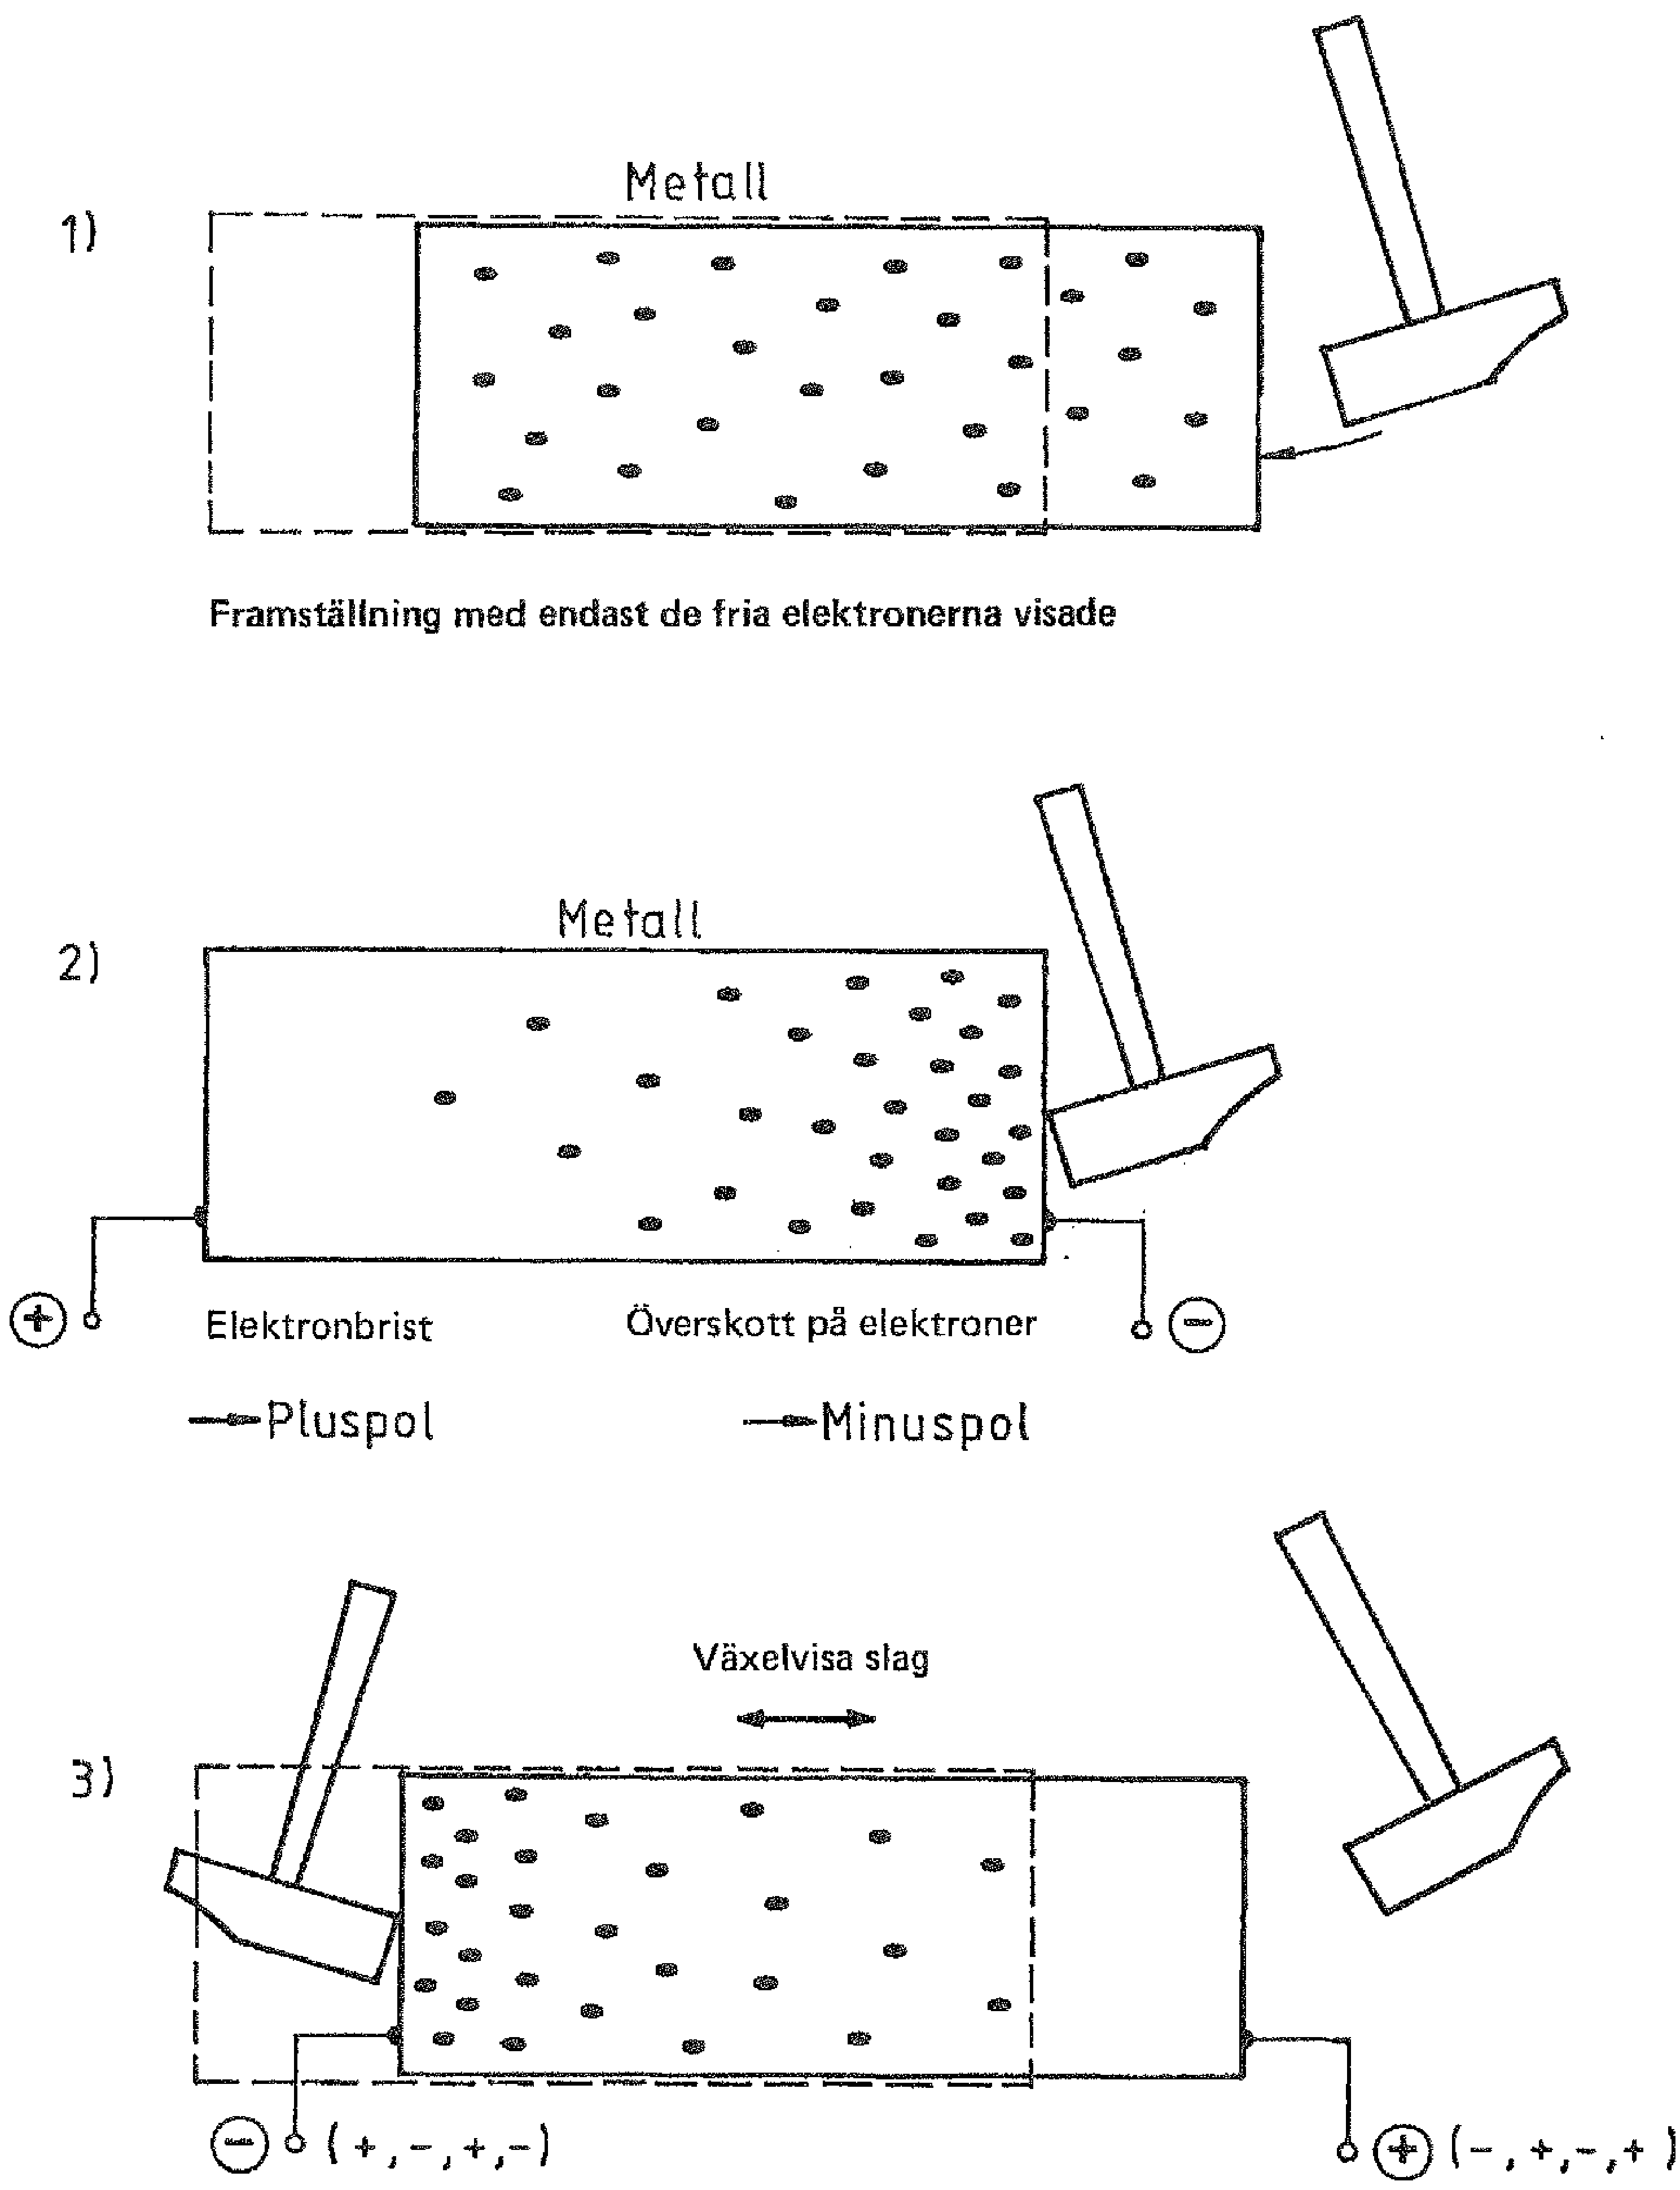
\includegraphics[width=\textwidth]{images/cropped_pdfs/bild_2_1-02.pdf}
\caption{Tankeförsök med kulor i ett rör}
\label{fig:BildII1-2}
\end{center}
\end{figure*}

Bild \ref{fig:BildII1-2} illustrerar ett tankeförsök med ett rör med kulor i. Materialet i röret tänks motsvara atomstrukturen i en strömledare och kulorna
de fria elektronerna.
Tänker man sig ett slag mot en ände av röret så flyttar det sig av den energi
som tillförs.
På grund av obundenheten till röret följer av masströgheten kulorna inte med
röret, utan hamnar i dess ena ände.

Att kulorna samlas i ena änden av röret tänks motsvara ett elektronöverskott i
ena änden av en ledare och ett motsvarande underskott i den andra änden.

Man kallar änden med elektronöverskott för minuspol och änden med
elektronunderskott för pluspol.
Olika stora elektriska laddningar vid polerna innebär att de sinsemellan har
olika potential.
Potentialskillnaden kallas spänning.

Likspänning innebär ett överskott av elektroner och alltid vid samma
anslutningspol.

Växelspänning innebär ett överskott av elektroner, omväxlande vid den ena
anslutningspolen och den andra.

Måttenheten för spänning är \(\mathrm{volt\ [V]}\).
I formler betecknas spänning med
\begin{itemize}
  \item \(U\) för effektivvärdet
  \item \(u\) för momentanvärdet (ögonblicks-)
  \item \(\hat{u}\) för toppvärdet (amplitud-).
\end{itemize}
Bild \ref{fig:BildII1-16} i avsnitt 1.6 illustrerar relationen mellan värdena
för en sinuskurva.

Spänningen över ändpunkterna på en strömledare är \(1\ \mathrm{volt\ [V]}\), då
ledaren genomflyts av en likström av \(1\ \mathrm{ampere\ [A]}\) under
effektutvecklingen \(1\ \mathrm{watt\ [W]}\).

\subsection{Symboler}

\begin{wrapfigure}[6]{R}{0.4\textwidth}
  \begin{mdframed}
    \centering
    \begin{circuitikz}
      \draw
      (4,1) to[battery1] (1,1)
      ;
    \end{circuitikz}
    \caption{Schemasymbol för batteri}
    \label{fig:bildII2-batteri}
  \end{mdframed}
\end{wrapfigure}

\textbf{FÖRDJUPNING}

När man ritar scheman för elektriska kretsar används symboler.
Symbolen i bild \ref{fig:bildII2-batteri} visar ett elektriskt batteri med en
enda cell.

Förtydligande kommentarer och skrivtecknen invid symbolen förekommer.
Ofta refererar dessa till en komponentlista.
Se även kapitel \ref{komponenter}.

\subsection{Elektrisk ström -- Enheten ampere}
\textbf{HAREC a.\ref{HAREC.a.1.1.2}\label{myHAREC.a.1.1.2a}, a.\ref{HAREC.a.1.1.3}\label{myHAREC.a.1.1.3a}}
\index{elektrisk ström}
\index{ström}
\index{ampere (A)}
\index{enheter!ampere (A)}
\index{symbol!\(I\) ström}

När en sluten strömkrets innehåller en spänningskälla, kan en
laddningsutjämning ske genom kretsen.
Det innebär att fria elektroner förflyttar sig genom kretsen i riktning från
spänningskällans minuspol till dess pluspol.
Vid pluspolen är det nämligen brist på negativa laddningar och naturen söker
alltid en utjämning.
Under utjämningsförloppet är spänningskällan även en strömkälla.

I gaser och elektrolyter (elektriskt ledande vätskor och geler) samt i
halvledare består strömmen av joner (positiva eller negativa laddningar), i metaller däremot av elektroner (negativa laddningar).

Av tradition anses strömriktningen vara positiv i jonströmmens riktning -- den
s.k. tekniska strömriktningen -- medan elektronströmmens riktning är den
motsatta -- den s.k. fysikaliska strömriktningen.

Måttenheten för ström är \emph{ampere} \(\mathrm{A}\) \cite{SIbrochure8}.

I formler betecknas ström med
\(I\) för effektivvärdet,\\
\(i\) för momentanvärdet (ögonblicks-),\\
\(\hat{i}\) för toppvärdet (amplitud-).

Strömmen är \(1\ \mathrm{A}\) när \(6,25 \cdot 10^{18}\) elektroner per sekund
flyter genom ett givet ledartvärsnitt, vilket motsvarar laddningen
\(1\ \mathrm{coulomb}\).

\subsection{Strömkrets}
\textbf{FÖRDJUPNING}
\index{strömkrets}

\begin{figure*}
\begin{center}
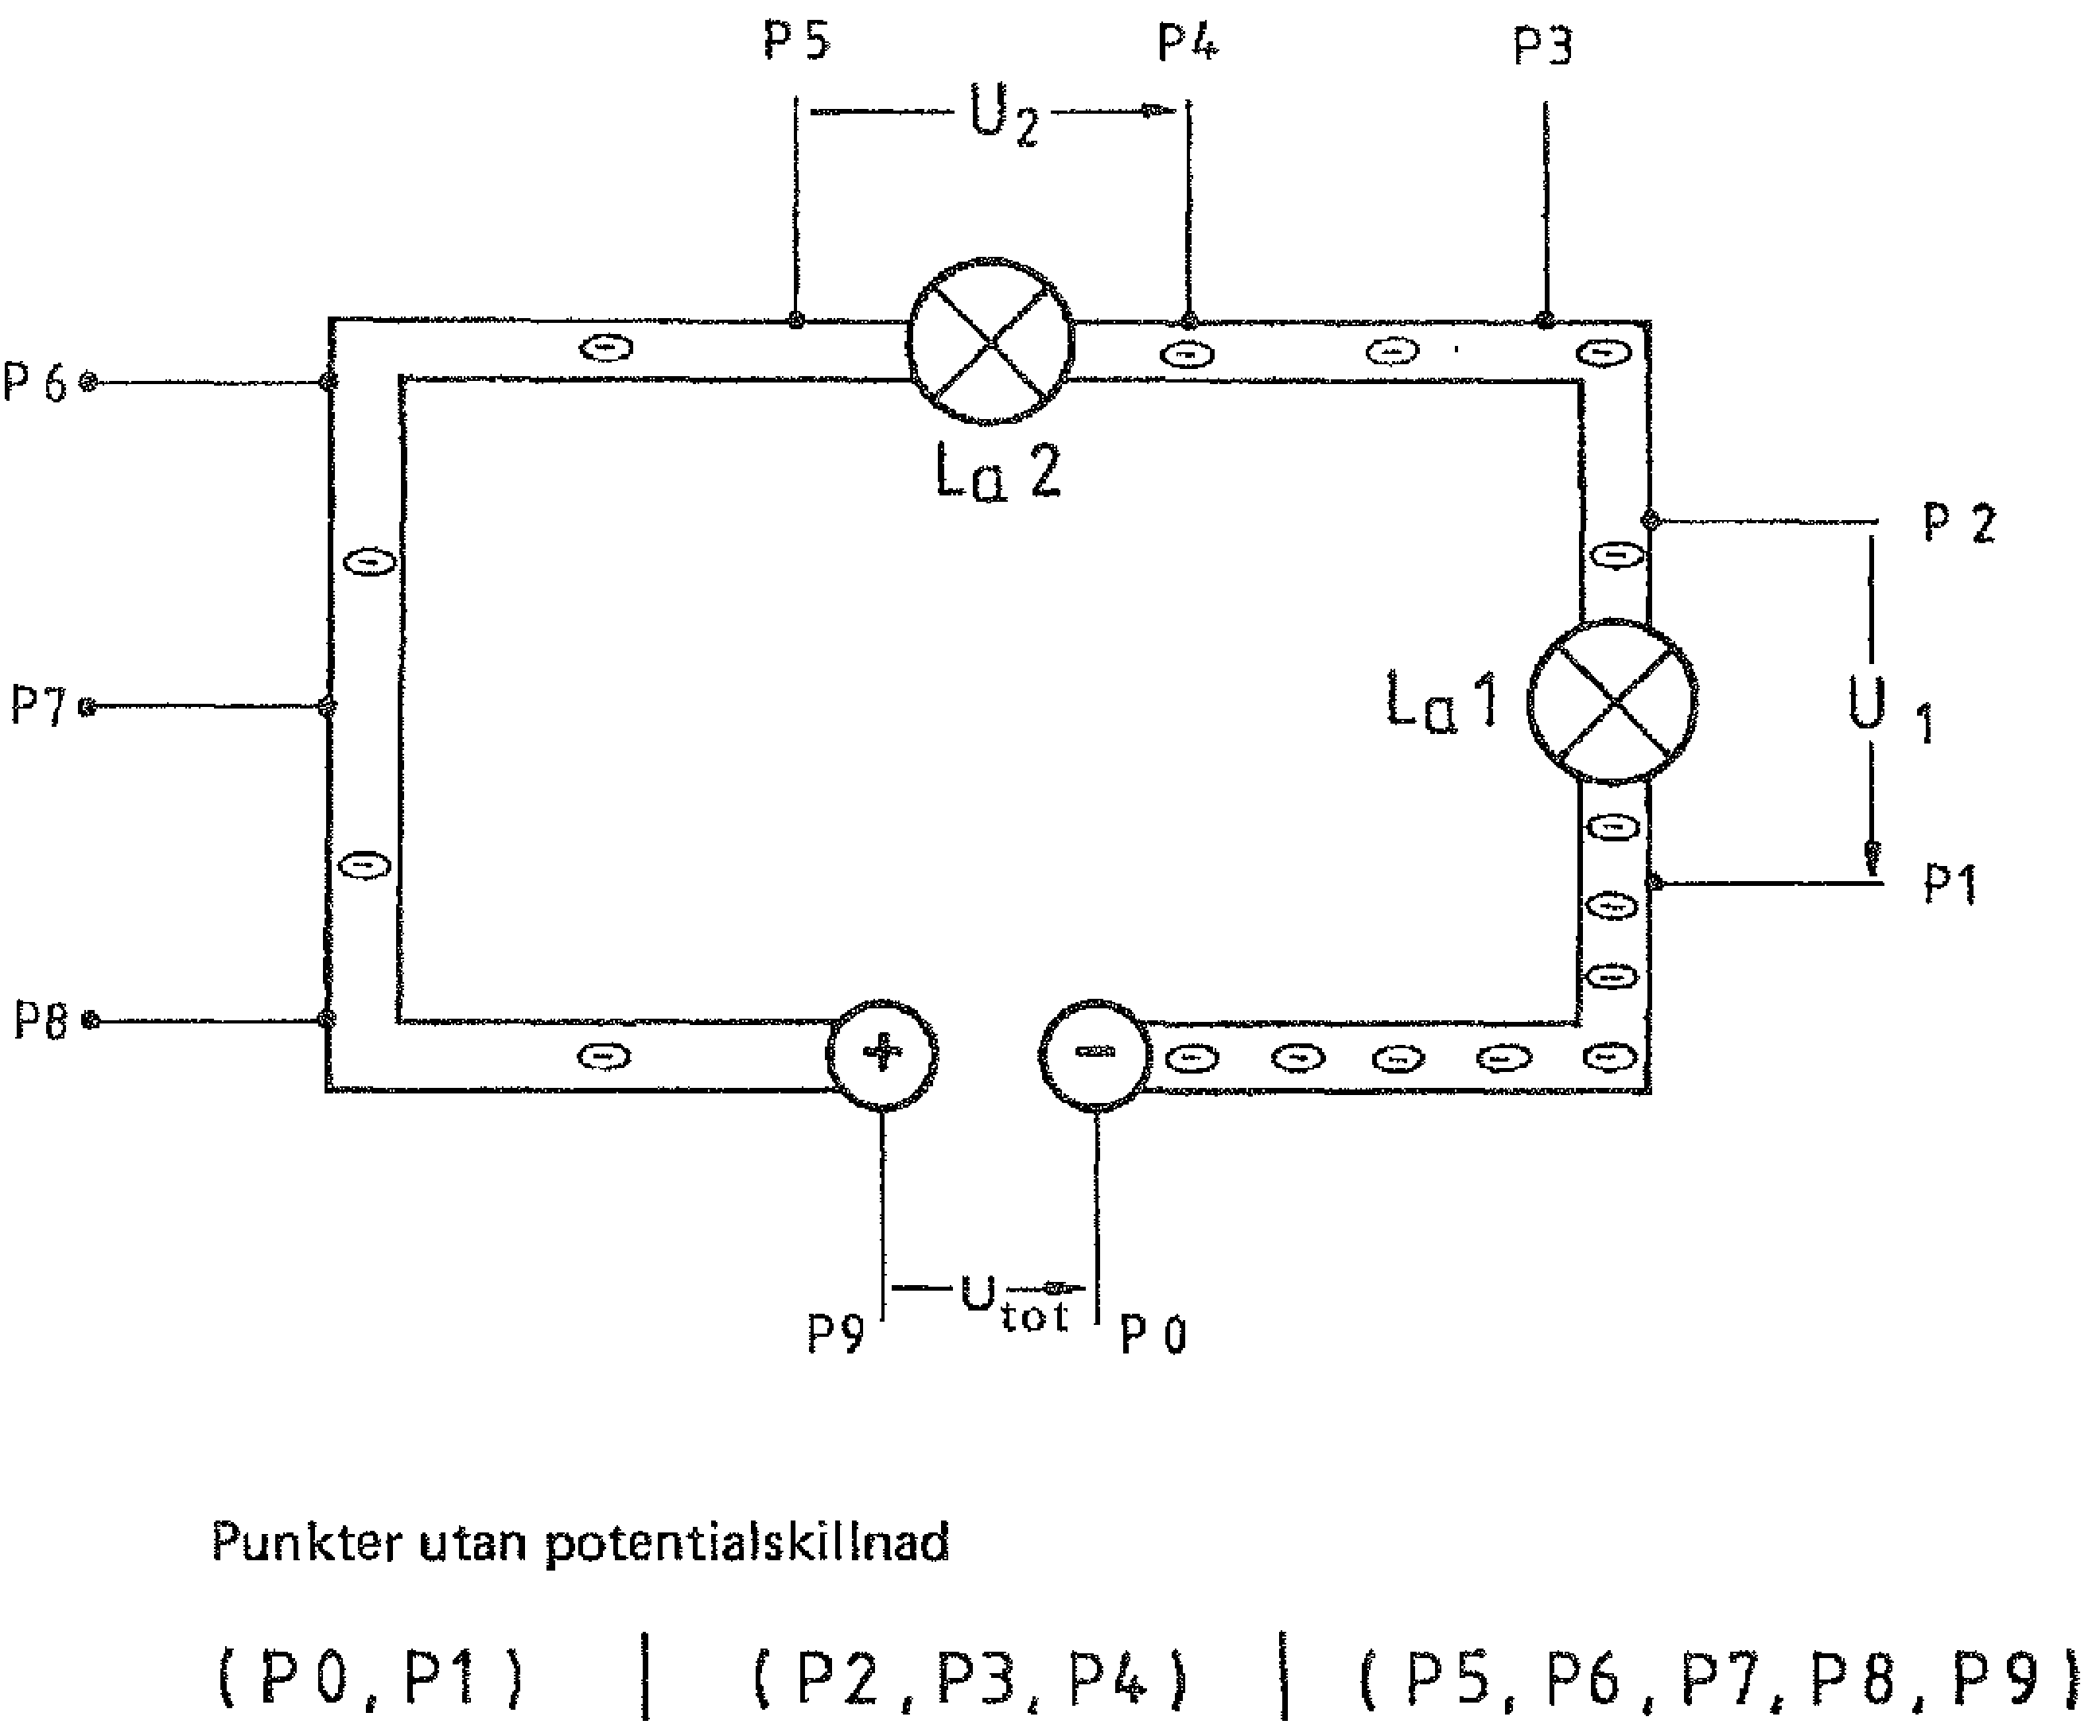
\includegraphics[width=0.6\textwidth]{images/cropped_pdfs/bild_2_1-03.pdf}
\caption{Potential och spänning i en strömkrets}
\label{fig:BildII1-3}
\end{center}
\end{figure*}

Bild \ref{fig:BildII1-3} visar potential och spänning i en strömkrets.

En elektrisk strömkrets består av en eller flera energikällor och
energiförbrukare.
Källor kan vara batterier, nätaggregat etc.
Förbrukare kan vara lampor, ledningar etc.
Varje energiförbrukare har en resistans och de elektriska laddningarna ''köar''
före förbrukaren, strax efter förbrukaren finns ingen kö.
Det uppstår en skillnad i laddningsmängd (en potentialskillnad) mellan varje
punkt i en strömkrets, när det flyter ström.
Man talar om spänningsfall.

\subsection{Strömförlopp}
\textbf{FÖRDJUPNING}
\index{strömförlopp}

Likströms- och växelströmsförloppen kan vara sammansatta av ett huvudförlopp och
underordnade förlopp.

Likström kan ha konstant styrka eller den kan variera enligt något förlopp, men
växlar aldrig riktning.

Växelström kan variera enligt något visst förlopp, t.ex. sinusvåg,
fyrkantsvåg, och växlar ständigt riktning.

\subsection{Resistans -- Enheten ohm}
\textbf{HAREC a.\ref{HAREC.a.1.1.2}\label{myHAREC.a.1.1.2c}, a.\ref{HAREC.a.1.1.3}\label{myHAREC.a.1.1.3c}}
\index{resistans}
\index{ohm (\(\Omega\))}
\index{enheter!ohm (\(\Omega\))}
\index{symbol!\(R\) resistans}

När fria elektroner tvingas fram genom atomstrukturen i en ledare, t.ex.
glödtråden i en lampa, så avgår energi i form av värme.
Detta fenomen kallas för resistans (av latinets resistere som betyder att
motstå).
Resistansen och därmed förlusterna i en strömkrets fördelas i
förhållande till de ingående materialen och deras dimensionering.

Resistans uttrycks i enheten \emph{ohm} \cite{SIbrochure8} och betecknas med
den grekiska bokstaven omega (\(\Omega\)).

I formler betecknas resistansen i en elektrisk krets eller en del av den med
\(R\).

Resistansen i en resistor är \(1\ [\Omega]\), när en spänning av \(1\ \mathrm{[V]}\)
driver en ström av \(1\ \mathrm{[A]}\) genom den resistorn.

\subsection{Ohms lag}
\textbf{HAREC a.\ref{HAREC.a.1.1.4}\label{myHAREC.a.1.1.4}}
\index{Ohms lag}
\index{resistor!Ohms lag}

Ohms lag beskriver sambandet mellan grundbegreppen ström
\(I\ \mathrm{[ampere]}\), spänning \(U\ \mathrm{[volt]}\) och resistans
\(R\ \mathrm{[ohm]}\).
Sambandet gäller både för likspänning och för effektivvärdet av växelspänning och
växelström.

I en ledare med resistansen \(R\) är strömstyrkan \(I\) genom resistansen
proportionell mot den pålagda spänningen \(U\).

\(
\begin{array}{lllll}U=I \cdot R & & I=\dfrac{U}{R} & & R=\dfrac{U}{I}\end{array}
\)

\subsection{Kirchhoffs lagar}
\textbf{HAREC a.\ref{HAREC.a.1.1.5}\label{myHAREC.a.1.1.5}}
\index{Kirchhoffs lagar}
\index{Kirchhoffs strömlag}
\index{Kirchhoffs spänningslag}

Den tyske fysikern G R Kirchhoff (1824--1887) formulerade sina välkända lagar
först 1845 och sedan 1847.

Kirchhoffs strömlag:

Den algebraiska summan av alla strömmar, som flyter till eller från varje punkt
i en elektrisk krets, är lika med noll.

\(I_1 + I_2 + I_3 + \cdots + I_n = 0\)

Kirchhoffs spänningslag:

I varje sluten strömkrets är den algebraiska summan av alla spänningskällor lika
med det totala spänningsfallet i alla resistorer.

Uttryckt på ett annat sätt är algebraiska summan av spänningarna i en
strömkrets lika med noll.

\subsection{Elektrisk effekt -- Enheten watt}
\textbf{HAREC a.\ref{HAREC.a.1.1.6}\label{myHAREC.a.1.1.6}, a.\ref{HAREC.a.1.1.7}\label{myHAREC.a.1.1.7}}
\index{elektrisk effekt}
\index{effekt}
\index{voltampere (VA)}
\index{enheter!voltampere (VA)}
\index{watt (W)}
\index{enheter!watt (W)}
\index{symbol!\(P\) effekt}

När en ström flyter genom en resistans utvecklas värme.
Värme är en form av effekt, som är högre ju starkare strömmen och högre
spänningen är.

Måttenheten \emph{voltampere} \(\mathrm{[VA]}\) för elektrisk effekt härleds ur
produkten av volt \(\mathrm{[V]}\) och ampere \(\mathrm{[A]}\).

För effekt som alstras av likström används enheten \emph{watt} \(\mathrm{[W]}\)
\cite{SIbrochure8} i stället för \emph{voltampere} \(\mathrm{[VA]}\).
Vid sidan om grundenheten \(1\ \mathrm{W}\) används delar och multipler av
denna.

\(1\ \mathrm{volt\ [U]}\ \cdot\ 1\ \mathrm{ampere\ [I]}\ =\ 1\ \mathrm{watt\ [P]}\)

Effektformeln \(P = U \cdot I\) gäller i första hand för likström men även för
växelström om belastningen är resistiv och ström och spänning inte är
fasförskjutna.
Formeln kan för att underlätta beräkningar skrivas om på flera sätt.

Vi börjar med att lösa ut \(I \quad \text{ur Ohms lag} \quad U = R \cdot I\) 

\(
I = \dfrac{U}{R}\\
\)

Vi sätter sedan in uttrycket för \(I\) i effektformeln

\(
\begin{array}{lllll}
P=U \cdot I & \Rightarrow & P= \dfrac{U \cdot U}{R} & \Rightarrow & P= \dfrac{U^2}{R}\\
\end{array}
\)

På motsvarande sätt kan vi ersätta \(U \quad\text{med}\quad R \cdot I\)

\(
\begin{array}{lllll}
P=U \cdot I & \Rightarrow & P = R \cdot I \cdot I  & \Rightarrow & P = R \cdot I^2\\
\end{array}
\)

Med hjälp av dessa formler kan effekten beräknas ur resistans- och strömvärdena
respektive ur resistans- och spänningsvärdena.
För övriga formler se formelsnurran bild \ref{fig:BildII1-4}

\subsection{Elektrisk arbete -- Enheten joule}
\textbf{FÖRDJUPNING}
\index{elektriskt arbete}
\index{joule (J)}
\index{enheter!joule (J)}
\index{symbol!\(W\) energi, arbete}

Energi finns i olika former, alltid och överallt.
Energi kan varken skapas eller förstöras, bara omvandlas från en form till en
annan.
Formen kan vara mekanisk, kemisk, elektrisk etc.

Arbete är omvandlingsprocessen från en energiform till en annan.

Arbetsmängden i alla energiformer kan mätas med samma enhet \emph{joule}
\(\mathrm{[J]}\) \cite{SIbrochure8} och anges med symbolen \(W\) för Work.

\(1\ \mathrm{joule}\) motsvarar det arbete som utvecklas när ett föremål
förflyttas \(1\ \mathrm{meter}\) med kraften \(1\ \mathrm{newton\ [N]}\),
d. v. s. \(1\ \mathrm{newtonmeter\ [Nm]}\).

\(W = l \cdot F \ \ \ \mathrm{[J] = [Nm]}\)

Arbetet \(W\ \mathrm{[J]}\) är mer ju längre tid \(t\ [s]\) en viss effekt
\(P\ \mathrm{[W]}\) utvecklas.

\(W = t \cdot P \ \ \ \mathrm{[J] = [sW]}\)
  
\subsection{Joules lag}
\textbf{HAREC a.\ref{HAREC.a.1.1.8}\label{myHAREC.a.1.1.8}}
\index{Joules lag}

\(Arbete\ =\ Effekt\ \cdot\ tid\ \ \ \mathrm{[W]} = \mathrm{[P]} \cdot \mathrm{[s]}\)

Eftersom effekten uttrycks som \(P = U \cdot I\) kan det elektriska arbetet
uttryckas som \(W = U \cdot I \cdot t\), vilket också är Joules lag.

Om grundenheterna för volt \(\mathrm{[U]}\), ampere \(\mathrm{[I]}\) och
sekund \(\mathrm{[s]}\) sätts in i formeln fås en måttenhet, uttryckt som
voltamperesekunder \(\mathrm{[VAs]}\) eller wattsekunder \(\mathrm{[Ws]}\)
eller joule\ \(\mathrm{[J]}\).

Måttenheten för elektriskt arbete är \(1\ joule\ per\ sekund\), som vanligen
kallas \(1\ \mathrm{wattsekund}\ \mathrm{[1\ Ws]}\).
Vid sidan av grundenheten används multipler av denna.
Exempel:
\(
\begin{array}{llll}
1\ \mathrm{kilowattsekund} & = 1\ \mathrm{kWs} & = 1\ 000\ \mathrm{Ws} & = 1,0 \cdot 10^3\ \mathrm{Ws}\\
1\ \mathrm{wattimme} & = 1\ \mathrm{Wh} & = 3\ 600\ \mathrm{Ws} & = 3,6 \cdot 10^3\ \mathrm{Ws} \\
1\ \mathrm{kilowattimme} & = 1\ \mathrm{kWh} & = 1 000\ \mathrm{Wh} & = 3,6 \cdot 10^6\ \mathrm{Ws}
\end{array}
\)

\subsection{Formelsnurran}
\index{formelsnurran}
\textbf{FÖRDJUPNING}

\begin{figure*}[ht]
\begin{center}
  %%\begin{wrapfigure}{R}{0.3\textwidth}
  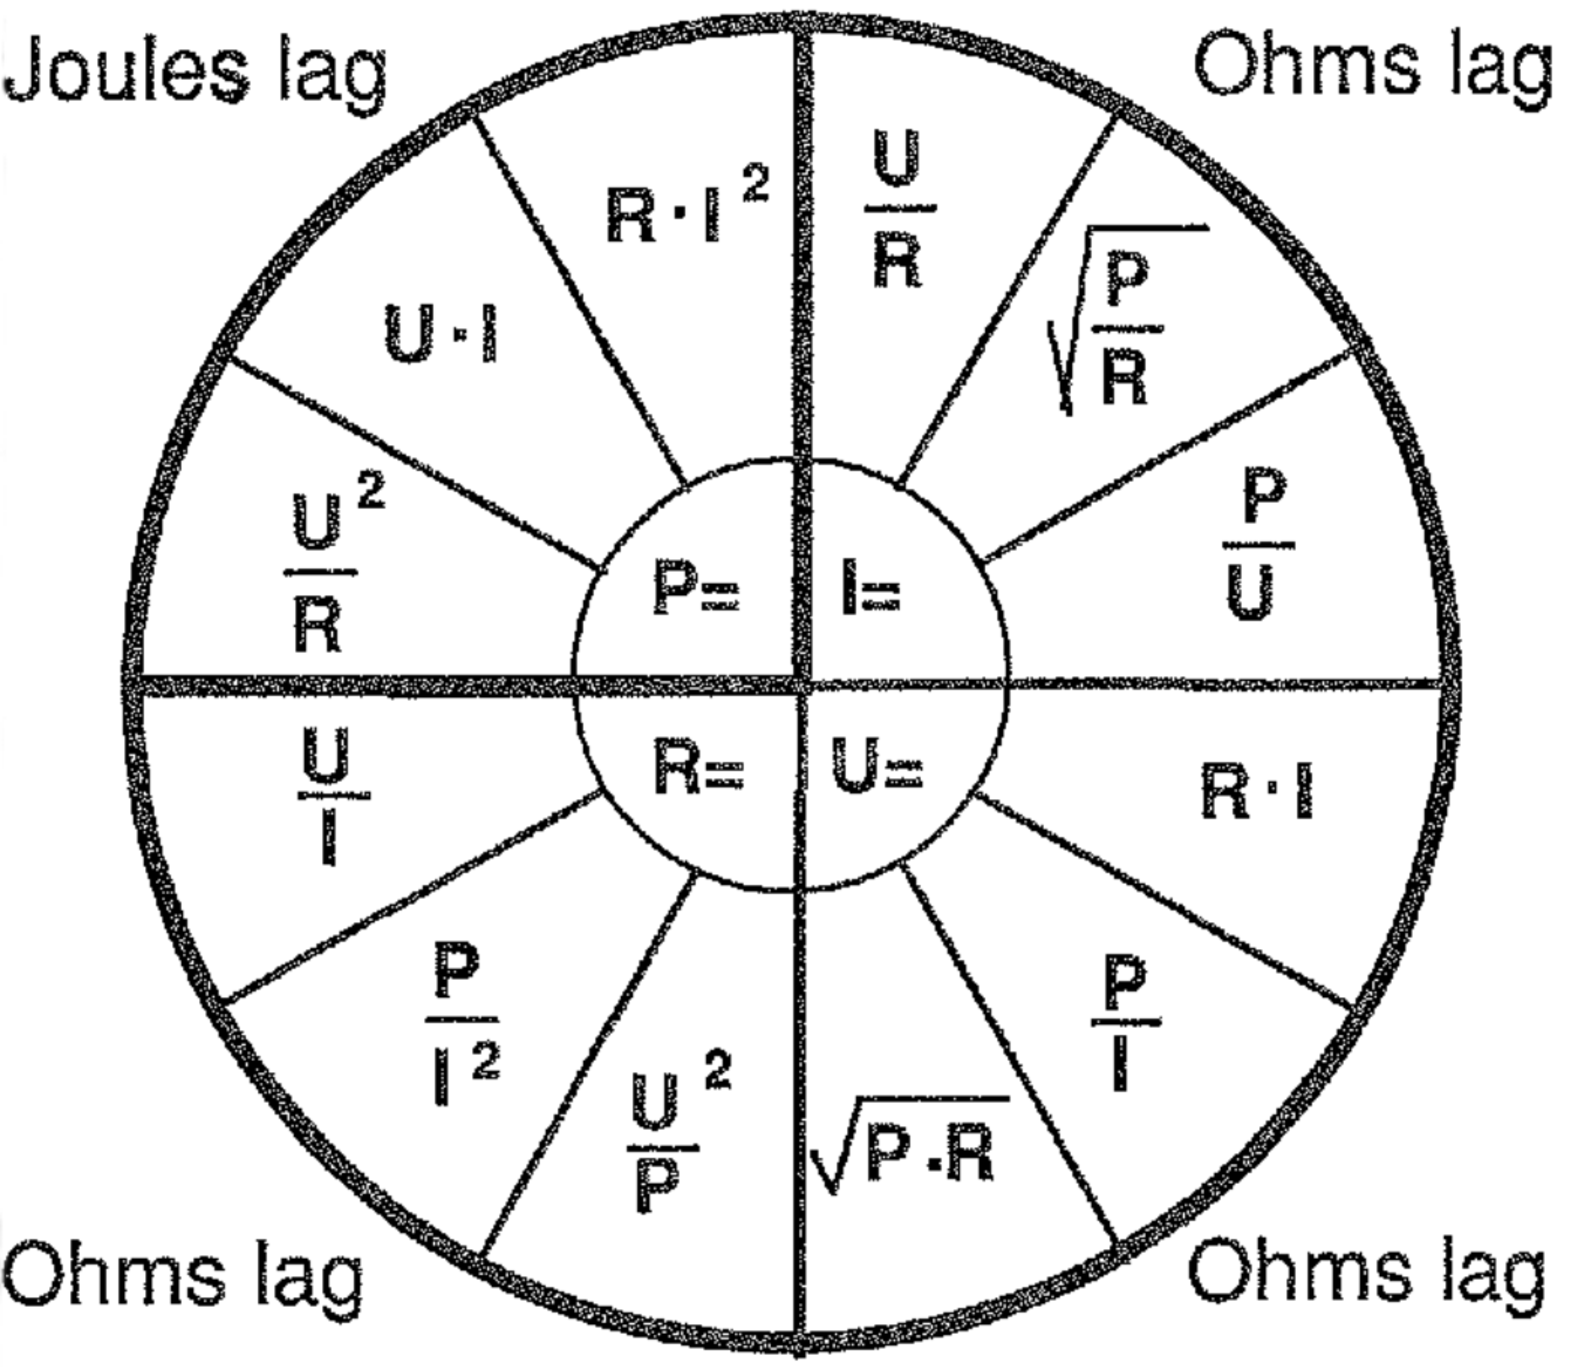
\includegraphics[width=0.5\textwidth]{images/cropped_pdfs/bild_2_1-04.pdf}
  \caption{''Formelsnurra'' för Ohms och Joules lagar}
  \label{fig:BildII1-4}
  %  \vspace{-100pt}
  %%\end{wrapfigure}
\end{center}
\end{figure*}

Så här finner man rätt formel i ''snurran'' (bild \ref{fig:BildII1-4}):
Välj ett segment med önskad storhet \(I\), \(U\), \(R\) eller \(P\) som det
första ledet i formeln.
Inom valt segment finns tre alternativ för det andra ledet i formeln.
Välj det alternativ som innehåller två kända storheter.

Bild \ref{fig:BildII1-4} visar ''Formelsnurra'' för Ohms och Joules lagar.

Exempel:

\subsubsection{Ohms lag}

\(R\) söks, \(U\) och \(I\) är kända;
Om \(U = 230\ V\) och \(I = 2\ A\), så blir

\(R=\dfrac{U}{I}=\dfrac{230}{2}=115\ \Omega\)

\subsubsection{Joules lag}

\(P\) söks, \(U\) och \(I\) är kända;

Om \(U = 230\ V\) och \(I = 2\ A\), så blir

\(P = U \cdot I = 230 \cdot 2 = 460\ W\)

\subsection{Amperetimmar (Ah) och batterikapacitet}
\textbf{HAREC a.\ref{HAREC.a.1.1.9}\label{myHAREC.a.1.1.9}}
\index{amperetimmar (Ah)}
\index{batterikapacitet}
\index{batteri}
\index{ackumulator}
\index{polspänning}
\index{elektrisk cell}

Det finns flera sätt att lagra energi.
Ett sätt är att göra det i kemisk form i speciella celler, där man kan ta ut
energin i elektrisk form.

Det finns celler som kan laddas upp och laddas ur upprepade gånger, s.k.
ackumulatorer.
Det finns också sådana celler som endast kan användas en gång och som inte
kan laddas upp igen, s.k. primärceller.

Energi i form av en elektrisk laddning kan även lagras i en kondensator.
Energin kan då lagras och tas ut utan omvandling.

Kapaciteten i en elektrisk cell uttrycks som produkten av den ström
\(\mathrm{[A]}\) som cellen avger och under den tid \(\mathrm{[s, h]}\) detta
kan ske.
Uttryckt med tidsenheten timmar blir då kapaciteten \(\mathrm{[Ah]}\).

Den kapacitet som anges i en cells produktdata är den nominella.
Denna kapacitet gäller endast under vissa normerade förhållanden såsom
celltemperatur, strömstyrka och urladdningstid.

Den praktiska kapaciteten i en cell begränsas av användningen.
En elektrisk cell avger sålunda regelmässigt mindre energimängd, ju högre
urladdningsströmmen är.
Kapaciteten i en elektrisk cell skiljer sig i det avseendet från den i
t.ex. en oljetank, där man kan ta ut lika mycket energimängd som man häller i
och oberoende av hur fort man gör det.

Elektriska celler kan samlas till s.k. batterier, varvid cellerna oftast
seriekopplas.
Batteriets polspänning är då summan av cellernas polspänningar.

Hur stort arbete ett batteri avger, beror såväl på hela batteriets
polspänning som på de enskilda cellernas kapacitet.
Exempel:
Ett batteri med polspänningen \(12\ \mathrm{V}\) och cellkapaciteten
\(100\ \mathrm{Ah}\) kan nominellt avge
\(P = U \cdot I = 12 \cdot 100 = 1200\ \mathrm{VAh} = 1,2\ \mathrm{kWh}\).

Hur länge batteriet ''räcker'' per laddning beror som sagt bl.a. på vilken
strömstyrka man tar ut.
Tar man ut \(1\ \mathrm{A}\) ur \(100\ \mathrm{Ah}\)-cellen här ovan, så blir
urladdningstiden nominellt
\(t = 100\ \mathrm{Ah}/1\ \mathrm{A} = 100\ \mathrm{h}\).

\section{Elektriska kraftkällor}
\textbf{HAREC a.\ref{HAREC.a.1.2}\label{myHAREC.a.1.2}}

\subsection{Elektromotorisk kraft -- EMK}
\textbf{HAREC a.\ref{HAREC.a.1.2.1}\label{myHAREC.a.1.2.1}}
\index{elektromotorisk kraft (EMK)}
\index{EMK}
\index{volt (V)}

Det som driver ström genom en elektrisk strömkrets är kretsens elektromotoriska
kraft (EMK).

Måttenheten för EMK är \(volt\ [V]\).

EMK är summan av de potentialökningar som uppstår i kretsen.

De vanligaste slagen av emk är
\begin{itemize}
\item elektromagnetisk emk som uppkommer i strömledare i magnetfält som
varierar (ex. lindningarna i en roterande generator)
\item elektrokemisk emk som uppkommer i beröringsytan mellan en metallisk
ledare och en elektrolyt (ex. battericell)
\item elektrostatisk emk, t.ex. i kondensatorer
\item kontaktemk i beröringsytan mellan metaller med olika termoelektrisk
potential eller mellan metall och luftens syre (ex. korrosion mellan metaller)
\item termoemk som uppkommer i en strömkrets där två sammanlödda metaller med
olika temperatur ingår (ex. termokors för strömmätning).
\end{itemize}

\subsection{Polspänning}

Den spänning, som kan mätas mellan kretsens anslutningspoler då kretsen är öppen.

\subsection{Inre resistans}

Liksom att komponenterna i strömkretsen har en viss resistans, så har också en
strömkälla en inre resistans.
Den inre resistansen i en strömkälla ingår i kretsens totala resistans.

\subsection{Kortslutningsström}

Om man på kortaste väg förbinder strömkällans anslutningspoler så blir kretsen
totala resistans lika med källans inre resistans.

Den kortslutningsström som då uppstår, begränsas enbart av strömkällans
polspänning och inre resistans.

Eftersom den inre resistansen oftast är mycket liten blir kortslutningsströmmen
motsvarande hög.

\subsection{Serie- och parallellkopplade kraftkällor}
\textbf{HAREC a.\ref{HAREC.a.1.2.2}\label{myHAREC.a.1.2.2}}

\subsubsection{Seriekopplade kraftkällor}

För att uppnå en högre total spänning (emk) kan flera kraftkällor
(delspänningar) kopplas i en slinga efter varandra. Detta kallas seriekoppling.

Seriekopplade delspänningar verkar med eller mot varandra, beroende på
deras inbördes polariteter.

Den totala spänningen över kopplingen är summan av de ingående
delspänningarna, med hänsyn taget till deras polariteter.

\subsubsection{Parallellkopplade kraftkällor}

För att erhålla högre ström, kan flera svagare kraftkällor parallellkopplas.
Vid parallellkoppling erhålls däremot inte högre spänning.

Vid parallellkoppling av kraftkällor \textbf{måste} deras polaritet vara lika.

För minsta utjämningsström mellan parallellkopplade kraftkällor bör även deras
polspänning och inre resistans vara så lika som möjligt.

\textbf{NOT: Parallellkoppling av kraftkällor är ofta olämpligt eftersom det
i praktiken är svårt att få en balans, varvid enbart den ena källan levererar.
Det finns kraftaggregat designade för att parallellkopplas.}

\section{Elektriskt fält}
\harec{a}{1.3}{1.3}
\label{elektriskafält}
\index{elektriska fält}

\subsection{Potential}
\index{elektrisk potential}

Potentialskillnaden -- spänningen -- mellan olika laddade kroppar skapar
krafter mellan varandra samt mellan dem och deras omgivning.
Detta fenomen kallas elektriskt kraftfält och är orsaken till att elektriskt
laddade kroppar kan komma i rörelse.

\subsection{Elektrisk laddning}
\index{elektrisk laddning}
\index{symbol!\(e\) elementarladdning}
\index{symbol!\(Q\) laddning}
\index{coulomb (C)}
\index{enheter!coulomb (C)}

Elektriska laddningar är grunden för elektricitetsläran.
Varje proton i atomkärnan är bärare av en positiv laddning.
Neutronerna i atomkärnan är elektriskt neutrala.
Antalet protoner i kärnan bestämmer därför kärnans totala positiva
laddning, kallat för kärnladdningstalet.
Elektronerna som kretsar omkring atomkärnan är bärare av var sin negativ
laddning.

Elementarladdningen [\emph{e}] är den laddning som finns i en elektron och har
länge ansetts vara den minsta möjliga laddningen.
Nutida elektronfysik konstaterar ännu mindre enheter, men det går vi inte in på
här.

Antalet protoner och elektroner i en atom är lika och elektronernas
negativa laddning blir då lika stor som protonernas positiva laddning.
När laddningar med olika polaritet är lika stora väger de ut varandra och blir
elektriskt neutrala till sin omgivning.

Måttenheten för elektrisk laddning är \(coulomb\ [C]\).
Laddningsmängden \(1\ coulomb\) motsvarar 6,25 triljoner (\(6,25\cdot10^{18}\))
elementarladdningar. Sambandet mellan laddning och ström är:
%%
\[Q = I \cdot t\]
%%
Laddning $[Q]$ är ström $[I]$ under tiden $[t]$:
%%
\[1\ C ~=~ 1\ A \cdot 1\ s ~=~ 1\ \textit{amperesekund}\ [1\ As]\]
\[1\ \textit{coulomb} ~=~ 1\ \textit{ampere} \cdot 1\ \textit{sekund}\]
%%

\smallfig{images/cropped_pdfs/bild_2_1-05.pdf}{Elektriska kraftfält}{fig:BildII1-5}

\subsection{Kraftfält omkring elektriska laddningar}

%%Bild \ref{fig:BildII1-5} visar elektriska kraftfält.

\noindent
Mellan elektriska laddningar bildas krafter (bild \ref{fig:BildII1-5}).

\begin{itemize}
  \item Varje laddning är omgiven av ett elektriskt kraftfält.
  \item Mellan positiva (+) elektriska laddningar och (--) negativa laddningar
  bildas krafter.
  \item Fältkrafternas styrka och riktning symboliseras som linjer mellan
  positiva och negativa laddningar, där styrkan är densamma utmed respektive
  linje.
\end{itemize}

%%(även 1.1) --- TODO: VA??

\begin{quote}
\emph{Kroppar med olika slags laddningar dras till varandra}

\emph{Kroppar med lika slags laddningar stöter bort varandra}

\emph{Oladdade kroppar påverkas inte och ger ingen kraftverkan.}
\end{quote}

\subsection{Elektrisk fältstyrka}
\harec{a}{1.3.1}{1.3.1}
\harec{a}{1.3.2}{1.3.2}
\index{elektrisk fältstyrka}
\index{symbol!\(E\) elektrisk fältstyrka}

\smallfig{images/cropped_pdfs/bild_2_1-06.pdf}{Elektrisk fältstyrka}{fig:BildII1-6}

I en trådformad ledare, som det flyter likström igenom, fördelas strömmen lika
över tvärsnittet.
Om ledaren i stället är ett tunt plan, så blir strömfördelningen annorlunda.
Bilden visar ett plan med två elektroder, som anslutits till en spänningskälla.
Utmed sträckan mellan elektroderna fördelas strömmen över planet så som
strömlinjerna på bilden.
Fördelningen beror på elektrodernas utformning och polaritet.
Strömtätheten är inte lika över hela planet, eftersom planet kan ses som många
parallellkopplade resistorer vars resistanser ökar med tilltagande
strömlinjelängd.

Strömtätheten i planet är större där resistansen mellan elektroderna är liten.
Närmast elektroderna där alla strömlinjer samlas är strömtätheten extremt hög.
Där strömtätheten är som störst finns den största potentialskillnaden
(spänningen) per längdenhet strömlinje.
Man kan mäta potentialerna i planet.
Spänningen mellan två punkter utmed en tänkt strömlinje är därvid proportionell
mot linjens längd mellan punkterna.
Halva spänningen finner man mitt emellan punkterna.

Elektriska fält är upplagrad energi.
Fältstyrkan kan bli så hög, att det blir en urladdning mellan polerna.
Koronaurladdning från ändarna av en antenn är ett annat tecken på hög
fältstyrka.
För att försvåra urladdning kan man öka elektrodytan, till exempel göra den klotformad.
Omvänt kan man medverka till urladdning genom att minska elektrodytan.
Ett exempel är åskledarens spets.

I bild \ref{fig:BildII1-6} \(U = f(l)\) visas spänningarna utmed
''mittströmslinjen'' igenom plus- och minuspolerna.
Kurvutseendet är typiskt även för omkringliggande linjer, oavsett längd.

Bilden framställer en ledare som ett idealt plan, medan den i praktiken är en
volym.
För att efterlikna en volym föreställer vi oss att bilden roterar omkring
mittströmslinjen, med fältlinjerna oförändrade.
Även om resistansen i den rotationskropp som uppstår är så hög att ingen ström
flyter, så är spänningsbilden fortfarande densamma.

Spänningsbilden gäller även för isolerande fasta material, gaser och vakuum.
Det finns alltså spänning mellan olika punkter även i ''friska luften''.
Denna spänningfältstyrka- kan mätas med särskilda instrument, så kallade
fältstyrkemätare.

Av brantheten på spänningskurvan i bilden framgår vilken delspänningen är per
dellängd av en spänningslinje.
Kvoten av delspänning och avståndet mellan mätpunkterna kallar man för
elektrisk fältstyrka.

I formler betecknas elektrisk fältstyrka med bokstaven \(E\).
Elektrisk fältstyrka mäts i volt per meter.
%%
\[
\begin{array}{ccc}
E=\dfrac{\Delta U}{\Delta l} &\quad& \dfrac{[volt]}{[meter]}
\end{array}
\]
%%
\subsection{Skärmning av elektriska fält}
\harec{a}{1.3.3}{1.3.3}
\index{elektriska fält!skärmning}
\label{elektrostatik skärmning}

I grunden finns det två slags fält, det elektriska och det magnetiska.
Dessutom finns det även elektromagnetiska fält, som är sammansatt av båda dessa.
Fält kan vara statiska eller dynamiska, varav här avses dynamiska.
Ett dynamiskt elektriskt fält genererar ett magnetiskt fält.
Omvänt generar ett dynamiskt magnetiskt fält ett dynamiskt elektriskt fält.
Denna växelverkan gör att fälten kan hållas igång av varandra med tillskott av
yttre energi.

Fält i rörelse alstrar elektromagnetisk strålning, som påverkar omgivningen.
När påverkan inte är önskvärd måste fältet skärmas av.
Ett sätt att skärma av ett elektriskt fält är en metallisk kapsling som
anslutits till apparatens jordreferens.
Skärmen behöver inte vara tät, men utförd så att all magnetiskt inducerad ström
i den bryts. (Jfr \ref{elektromagnetisk skärmning})

\section{Magnetiskt fält}
\harec{a}{1.4}{1.4}
\label{elektromagnetiskafält}
\index{elektromagnetiska fält}

\subsection{Magnetism}
\index{magnetism}
\index{Plinius}
\index{Magnes}
\index{Lithos herakleia}
\index{Herakleia}
\index{Magnesia}
\index{Magnetes}

\infobox{
Enligt den romerske författaren \emph{Plinius} lär, vid tiden ungefär
160~år f.Kr. herden \emph{Magnes} en dag ha känt hur järnstiften i
sandalerna häftade vid en viss sorts sten.
Det kunde ha varit svart järnmalm, som grekerna i äldsta tider benämnde
\emph{Lithos herakleia} efter staden \emph{Herakleia} i Lydien,
där sådan malm förekommer.
Staden fick sedermera namnet \emph{Magnesia} och man kan tänka sig att stenen
kom att kallas \emph{Magnetes}.
En hel mineralgrupp med liknande egenskaper, såsom järn, nickel m.fl. kallas
magnetiska.
}

\emph{Magnetism} uppstår av elektriska laddningar i rörelse.
Elektronernas rörelser i en atom skapar nämligen magnetfält.
Det gör att atomerna var för sig fungerar som en magnetisk dipol -- en magnet.
I de flesta material är atomerna orienterade så att deras magnetiska krafter
tar ut varandra.
Materialet som helhet är då omagnetiskt och utövar inga yttre krafter.
Men vid påverkan från ett yttre magnetfält kan dipolerna (atomerna) i ett
material orienteras i samma riktning och deras magnetfält kommer då att
samverka. Hela materialet blir då magnetiskt.
När det yttre magnetfältet avlägsnas, kvarstår orienteringen endast delvis --
\emph{magnetisk remanens}.
I ferromagnetiska legeringar kvarstår en större del av orienteringen, även om
påverkan från det yttre magnetfältet har upphört.
Materialet är då permanentmagnetiskt.

\subsection{Kraftfält i och omkring magneter}

\end{multicols}
\mediumfig{images/cropped_pdfs/bild_2_1-07.pdf}{Kraftfält omkring magneter}{fig:BildII1-7}
\begin{multicols}{2}

Bild \ref{fig:BildII1-7} visar kraftfält omkring magneter.
Varje magnet omges av ett magnetiskt kraftfält.
Magnetfältets fördelning, styrka och riktningar beskrivs som kraftlinjer med
slutna kretslopp.

Utanför magneten går kraftlinjerna från nord- till sydpol och inne i magneten
motsatt riktning.
Kraftriktningen i varje punkt av fältet är den som nordändan på en kompassnål
skulle peka åt.
Om man hänger upp en magnet i en tråd, så kommer den att inta samma riktning
som jordens magnetfält.

\begin{quote}
\emph{Poler med samma polaritet stöter bort varandra (repellerar).}

\emph{Poler med olika polaritet dras till varandra (attraherar).}
\end{quote}

\mediumfig[0.5]{images/cropped_pdfs/bild_2_1-08.pdf}{Magnetiska fält omkring strömledare}{fig:BildII1-8}

\subsection{Magnetiska fält omkring strömbanor}
\harec{a}{1.4.1}{1.4.1}

Bild \ref{fig:BildII1-8} visar magnetiska fält omkring strömledare.
Omkring varje ledare, som det flyter en elektrisk ström igenom, alstras det ett
magnetiskt kraftfält.
Magnetiska kraftlinjerna fördelar sig koncentriskt omkring en rak ledare och
vinkelrätt mot denna.
Mellan ändarna av en ledare med bågformad utsträckning bildas kraftlinjer som
verkar med varandra.
En strömgenomfluten cylindrisk spole -- induktor -- uppvisar samma magnetiska
fältbild som en stavformad permanentmagnet.

\subsection{Bestämma magnetiska fältriktningen}

Magnetfältets riktning omkring en ledare kan enkelt bestämmas med
\emph{högerhandsregeln}.
När en \emph{ledare} fattas med höger hand och med tummen i strömmens
riktning, kommer fingrarna att peka i fältriktningen (B).

I bild \ref{fig:BildII1-8} (övre) så går strömmen från pluspolen (+) till
minuspolen (--) varvid strömmen kommer gå nedåt i bilden på ovansidan,
det vill säga precis så tummen pekar om man greppar ledaren med tummen nedåt,
och magnetfältet kommer att snurra som pilarna precis som de övriga fingrarna
på högerhanden.

När en ledare formas som en spole och en elektrisk ström flyter genom den,
kommer magnetfältet att ha ett utseende som liknar det omkring en
permanentmagnet.
En sådan spole kallas \emph{elektromagnet}.

Magnetfältets riktning i en spole kan också bestämmas med högerhandsregeln.
När \emph{en spole} fattas med höger hand och med fingrarna i strömmens
riktning, kommer den utsträckta tummen att peka mot spolens nordpol.

I bild \ref{fig:BildII1-8} (undre) så går strömmen från pluspolen (+) till
minuspolen (--) varvid strömmen kommer gå inåt i bilden på ovansidan, dvs.
precis så fingrarna pekar när man lägger handen på spolen, och magnetfältet
kommer att peka mot nord (N) precis som tummen på högerhanden.

Fälten omkring alla slags magneter, såväl permanentmagnetiska som
elektromagnetiska, återverkar på varandra.
Även enkla elektriska ledare är elektromagneter.

\subsection{Exempel på elektromagneter}

\tallfig{images/cropped_pdfs/bild_2_1-09.pdf}{Exempel på elektromagneter}{fig:BildII1-9}

Bild \ref{fig:BildII1-9} visar exempel på elektromagneter.

\subsubsection{Elektromagnet}
Det bildas ett magnetfält genom en spole så länge som det flyter ström genom
den.
En järnkärna i spolen koncentrerar fältet på grund av den större magnetiska
ledningsförmågan.

Elektromagneter används för att sätta magnetiska material i rörelse eller hålla
fast dem.

\subsubsection{Elektrisk ringklocka}
Anordningen består av en elektromagnet och en järnplatta på en fjäder.
På plattan sitter en självbrytande kontakt samt en kläpp som kan slå på en
klocka.

Kontakten åstadkommer en växelvis brytning och slutning av strömmen genom
elektromagneten.
Armaturen med kläppen kommer då i svängning och slår på klockan.

\subsubsection{Telefon}
I en enkel telefon finns bland annat en mikrofon, ett batteri och en
hörtelefon.

Särskilt i äldre telefoner består mikrofonen av en kolkornskammare med ett
membran.
Tryckvariationer (ljud) får membranet att vibrera, varvid resistansen genom
kolkornen varierar i motsvarande grad.
Därmed varierar talströmmen genom mikrofonen.

Hörtelefonen består av en elektromagnet och ett membran av mjukjärn.
Variationer i talströmmen genom mikrofonen passerar även hörtelefonen och får dess
magnetfält att variera.
Hörtelefonens membran alstrar då trycksvariationer, det vill säga ljud.

\subsubsection{Elektromagnetiskt relä}
Reläet består av en elektromagnet, en järnplatta (ankare) på en fjäder och en
elektrisk kontakt.
Med en svag ström / låg spänning genom spolen i manöverkretsen kan man med
reläets arbetskontakt styra starkare ström / högre spänning i huvudkretsen.

\subsection{Magnetisk fältstyrka}
\index{magnetisk fältstyrka}
\index{symbol!\(H\) magnetisk fältstyrka}

Som magnetisk fältstyrka förstår man flödet per meter fältlinje, det vill säga

\begin{align*}
  &H = \frac{\Theta}{l} = \frac{I \cdot N}{l} \\
  &H\ [A/m] \\
  &I\ [A] \\
  &N\ \text{[varvtal]} \\
  &l\ \text{[fältlinjelängd]}
\end{align*}

\emph{Magnetisk fältstyrka uttrycks således som ampere per meter flödesväg.}

\subsection{Magnetisk flödestäthet}
\index{magnetisk flödestäthet}
\index{tesla (T)}
\index{enheter!tesla (T)}
\index{symbol!\(B\) magnetisk flödestäthet}
\index{permabilitet}
\index{symbol!\(\mu\) permabilitet}

\emph{Den magnetiska flödestätheten mäts i enheten tesla \([T]\) (förut gauss).}

Formeltecknet/symbol är \(B\).

Formeln är \(B = \mu \cdot H\)

Flödestäthet \(B\ [Vs/m^2]\) Fältstyrka \(H\ [A/m]\)

\(\mu\) är permabilitetstalet för materialet.
\(\mu_0\) är permeabilitetstalet (fältkonstanten) för den magnetiska
ledningsförmåga för vakuum.

För järn eller annat magnetiskt ledande material tillkommer permeabilitetstalet
\(\mu_r\).
Det anger hur många gånger bättre än luft etc., som materialet leder ett
magnetisk flöde.
Permabilitetstalet kan då skrivas
\(\mu = \mu_r\mu_0\).

Formeln är \(B = \mu_0 \cdot \mu_r \cdot H\)

\subsection{Magnetiskt flöde}
\index{magnetiskt flöde}
\index{symbol!\(\Phi\) magnetiskt flöde}

Det magnetiska flödet är produkten av flödestätheten \(B\) och tvärsnittsytan
\(A\) av flödesvägen, således

\(\Phi = B \cdot A\)

\(\Phi \text{[weber eller Vs]}\) \(B \text{[T eller tesla]}\) \(A [m^2]\)

\subsection{Skärmning av magnetiska fält}
\harec{a}{1.4.2}{1.4.2}
\index{magnetiska fält!skärmning}
\label{elektromagnetisk skärmning}

I grunden finns det två slags fält, det elektriska och det magnetiska. Det
finns även elektromagnetiska fält som är sammansatta av båda dessa.
Fält kan vara permanenta eller rörliga, varav här avses de rörliga.
Ett rörligt magnetiskt fält genererar ett elektriskt fält.
Omvänt generar ett rörligt elektriskt fält ett rörligt magnetiskt fält.
Denna växelverkan gör att fälten kan hållas igång med tillförsel av yttre
energi.

Fält i rörelse alstrar elektromagnetisk strålning, som påverkar funktioner i
omgivningen.
När påverkan inte är önskvärd, måste fältet skärmas av.
Ett sätt att skärma magnetiska fält är en metallisk kapsling.
Kapslingen ska vara tät och bilda en sluten magnetisk krets.
Kapslingen ska vara utförd i ett material som är en god ledare av magnetiskt
flöde.
(Jämför \ref{elektrostatik skärmning})

\section{Elektromagnetiska vågor}

\smallfig{images/cropped_pdfs/bild_2_1-10.pdf}{Vågor längs en linje}{fig:BildII1-10}

\harec{a}{1.5}{1.5}
\index{elektromagnetiska fält}

\subsection{Vågutbredning}
\harec{a}{1.5.1}{1.5.1}
\index{vågutbredning}

En tillståndsändring i ett medium innebär att energi tillförs eller tas bort.
Om detta sker växelvis uppstår förlopp såsom pendling, svängning, vågbildning etc.
Eftersom naturen söker jämvikt, så breder förloppet ut sig genom mediet efter
någon modell.

Energi kan inta olika tillstånd. I en pendel växlar energin mellan lägesenergi
och rörelseenergi.
Vågor på en vätskeyta liksom fjädring i fasta material är exempel på detta.
Det kan även innebära trycksvängningar i gaser och så vidare.

I detta avsnitt behandlas elektromagnetiska fält.
Sådana uppstår av svängningar i elektriska och magnetiska fält.
För att förklara pendling och utbredning används här modeller.

\subsection{Utbredningsmodeller}

\subsubsection{Vågutbredning längs en linje}

\smallfig{images/cropped_pdfs/bild_2_1-11.pdf}{Vågutbredning på en yta}{fig:BildII1-11}

Bild \ref{fig:BildII1-10} visar vågor längs en linje.
När änden av en tråd sätts i pendling med en frekvens \(f\), så kommer till
sist hela tråden i svängning med den frekvensen.
Den pendling, som först skapades, vandrar längs tråden med
utbredningshastigheten \(v\).
Våglängden är \(\lambda\) (lambda), som är avståndet mellan två närliggande
punkter med samma svängningsläge och svängningsriktning.

\subsubsection{Vågutbredning på en yta}
\index{vågutbredningshastighet}
\index{symbol!\(v\) vågutbredningshastighet}

Bild \ref{fig:BildII1-11} visar vågutbredning på en yta.
När ett föremål släpps genom en vätskeyta, så bildas vågor som breder ut sig
som cirklar i varandra (koncentriska).

De punkter på vågen, som för ögonblicket har samma svängningsläge, och är lika
långt från energikällan, kallas för vågfront.

Sambandet mellan utbredningshastighet \(v\), våglängd \(\lambda\) och frekvens
\(f\) är:
%%
\[
\begin{array}{llll}
v = \lambda \cdot f & v \ [m/s] & \lambda \ [m] & f \ [Hz=1/s]
\end{array}
\]
%%
Exempel: När våglängden \(\lambda = 2\ m\) och antalet svängningar per sekund
\(f = 10\ Hz\), så breder vågen ut sig med hastigheten \(v = 20\ m/s\).

\smallfig{images/cropped_pdfs/bild_2_1-12.pdf}{Vågutbredning i rummet}{fig:BildII1-12}

\subsubsection{Vågutbredning i rummet}

Bild \ref{fig:BildII1-12} visar vågutbredning i rummet.

Ljud är energi i form av tryckvågor i luften.
När en mekanisk kropp sätts i svängning (stämgaffel, dricksglas etc), överförs
svängningarna till den omgivande luftmassan som börjar att svänga med.
I luftmassan bildas det omväxlande över- och undertryckszoner, som breder ut
sig åt alla håll.
De mekaniska svängningarna i ljudkällan omvandlas alltså till tryckvågor.

Det mänskliga örat uppfattar tryckvågor inom frekvensområdet ca
15-\SI{18000}{Hz} som ljud.
Dessa vågor kallas ljudvågor.
Utbredningshastigheten för ljudvågor är \(v = \text{ca } 340\ \text{m/s}\) vid
15~\degree C och normalt lufttryck.

\subsection{Elektromagnetiska fält}
\harec{a}{1.5.2}{1.5.2}
\index{elektromagnetiska fält}

Tabell \ref{tab:elektromagnetiskt_spektrum} visar elektromagnetiskt spektrum.
I detta avsnitt görs i huvudsak endast jämförelse mellan ljusvågor och
radiovågor, vilka båda är elektromagnetisk strålning.
Hur ett elektromagnetiskt fält frigörs från en ledare framgår av kapitel
\ref{vågutbredning}.

Elektromagnetiska fält är energi, som är sammansatt av mycket snabbt svängande
elektriska och magnetiska fält.
När elektrisk ström genom en ledare ändras i styrka bildas ett magnetfält
omkring ledaren.
Detta magnetfält alstrar en elektromotorisk kraft (EMK), som är motriktad den
som driver fram strömmen.
Magnetfältet motverkar således strömändringen.
På liknande sätt alstrar en ändring av magnetfältet omkring ledaren en EMK i
form av ett elektriskt fält.
Detta driver en motriktad ström och därmed ett motverkande magnetiskt fält.

Både det elektriska och det magnetiska fältet har således alstrats av ändringar
i det andra och existerar därför bara tillsammans.

De båda fälten kombineras till ett elektromagnetiskt fält, som har egenskapen
att kunna stråla (breda ut sig) i alla tre dimensioner.
Beroende på frekvensen har elektromagnetiska fält olika egenskaper och
användning, vilket framgår av bilden.

\begin{table}
\begin{center}
\begin{tabular}{|rl|rl|l|}
\hline
\multicolumn{2}{|c|}{\multirow{2}{*}{Frekvens}} & \multicolumn{2}{c|}{\multirow{2}{*}{Våglängd}} & \multicolumn{1}{c|}{Egenskaper/} \\
 & & & & \multicolumn{1}{c|}{användning} \\ \hline
300 & Hz  & 100 & mil & \\
  1 & kHz & 300 & km & ULF \\ \cline{5-5}
  3 & kHz & 100 & km & \\
 10 & kHz &  30 & km & VLF \\ \cline{5-5}
 30 & kHz &  10 & km & \\
100 & kHz &   3 & km & LF \\ \cline{5-5}
300 & kHz &   1 & km & \\
  1 & MHz & 300 & m & MF \\ \cline{5-5}
  3 & MHz & 100 & m & \\
 10 & MHz &  30 & m & HF \\ \cline{5-5}
 30 & MHz &  10 & m & \\
100 & MHz &   3 & m & VHF \\ \cline{5-5}
300 & MHz &   1 & m & \\
  1 & GHz & 300 & mm & UHF \\ \cline{5-5}
  3 & GHz & 100 & mm & \\
 10 & GHz &  30 & mm & SHF \\ \cline{5-5}
 30 & GHz &  10 & mm & \\
100 & GHz &   3 & mm & EHF\\ \cline{5-5}
300 & GHz &   1 & mm & \\\
  1 & THz & 300 & \(\mu\)m & Infrarött \\
  3 & THz & 100 & \(\mu\)m & ljus \\
 10 & THz &  30 & \(\mu\)m & (värme- \\
 30 & THz &  10 & \(\mu\)m & strålning) \\
100 & THz &   3 & \(\mu\)m & \\ \cline{5-5}
300 & THz &   1 & \(\mu\)m & Synligt ljus \\ \cline{5-5}
  1 & PHz & 300 & nm & \\
  3 & PHz & 100 & nm & Ultraviolett \\
 10 & PHz &  30 & nm & ljus \\ \cline{5-5}
 30 & PHz &  10 & nm & \\
100 & PHz &   3 & nm & Rönt-\\
300 & PHz &   1 & nm & gen-\\
  1 & EHz & 300 & pm & strålning\\ \cline{5-5}
  3 & EHz & 100 & pm & \\
 10 & EHz &  30 & pm & Gamma-\\
 30 & EHz &  10 & pm & strål-\\
100 & EHz &   3 & pm & ning\\
300 & EHz &   1 & pm & \\
\hline
\end{tabular}
\end{center}
\caption{Elektromagnetiskt spektrum}
\label{tab:elektromagnetiskt_spektrum}
\end{table}

\subsubsection{Ljusvågor}
\index{ljusvågor}
\index{ljushastighet}
\index{symbol!\(c\) ljushastighet i vakuum}
\index{symbol!\(\lambda\) våglängd}

Ögat uppfattar elektromagnetisk strålning bara inom ett visst frekvensområde
som ljus.
Ljusets utbredningshastighet beror av vilket material, som det passerar igenom.
I vakuum är hastigheten störst, \(c = 299\, 792\, 458\ m/s\)
(= ca \(3 \cdot 10^8\ m/s\)) \cite{SIbrochure8}.
I tätare ämnen är hastigheten lägre, till exempel i glas ca \(200\, 000\, 000\ m/s\).
Det för människan synliga ljuset har våglängder mellan \(7,7 \cdot 10^{-7}\)
och \(3,9 \cdot 10^{-7}\ m\), motsvarande 7,7 till 3,9 tiotusendels mm.

Sambandet mellan ljusets utbredningshastighet \(c\) i vakuum, frekvensen \(f\)
och våglängden \(\lambda\) är
%%
\[
\begin{array}{llll}
c = \lambda \cdot f & c \ [m/s] & \lambda \ [m] & f \ [Hz]
\end{array}
\]
%%
\subsubsection{Radiovågor}
\index{radiovågor}

Även radiovågor är elektromagnetisk strålning, men inom ett lägre
frekvensområde än det för ljus.
Men utbredningshastigheten för radiovågor genom olika material följer ändå
samma lagar som de för till exempel ljusets utbredning.

Radiovågor anses omfatta ett frekvensområde från ca 10~kHz
(\(\lambda = 30\ km\)) till 300~GHz (\(\lambda = 1\ mm\)).

Rundradio tilldelas frekvenser i intervallet 100~kHz till 1000~MHz.
Amatörradio tilldelas ett antal frekvensområden i intervallet 1,8~MHz till
250~GHz.

Att märka är att elektromagnetiska fält, som sagts ovan, förekommer så långt
ner i frekvens som ett fåtal kHz.
Detta ska självklart inte förväxlas med ljudtryck med samma frekvens.

\subsubsection{Egenskaper hos elektromagnetiska vågor}

Elektromagnetiska vågor med högre frekvens än radiovågor uppfattas som
värmestrålning, vågor med ännu högre frekvens som ljus etc., men fortfarande är
huvudegenskaperna samma.
Som exempel kan nämnas polariserade vågor.
Dessutom kan man finna motsvarigheten till sådana egenskaper såsom interferens
och överlagring även i andra vågtyper, till exempel i ljud.

\subsection{Vågpolarisation}
\harec{a}{1.5.3}{1.5.3}
\label{vågpolarisation}
\index{vågpolarisation}

\largefig{images/cropped_pdfs/bild_2_1-14.pdf}{Polarisation av elektromagnetiska vågor}{fig:BildII1-14}

Bild \ref{fig:BildII1-14} visar polarisation av elektromagnetiska vågor.

\subsubsection{Vågor längs en linje (tråd e.d.)}
En vågrörelse i ett plan kallas linjärt polariserad.
Om änden på en horisontell tråd sätts i rörelse uppåt-nedåt, uppstår på tråden
en linjärt polariserad vågrörelse i vertikalplanet -- vertikal polarisering.
Om tråden sätts i rörelse höger-vänster kommer dess svängning att vara
horisontellt polariserad.
Om tråden sätts i svängning i ett plan och detta plan ständigt vrider sig,
kommer även vågrörelsen utmed tråden att vrida sig.
En vågrörelse, vars polarisering vrider sig roterar -- kallas för cirkulärt
polariserad.
Vridning mot- respektive medurs kallas för vänster- respektive högervriden
polarisering.

\subsubsection{Elektromagnetiska vågor}

De magnetiska och elektriska fälten omkring en ledare är vinkelrätt orienterade
mot varandra.
Det elektromagnetiska fält som de bildar tillsammans bildar en vågfront som
är vinkelrätt orienterad mot dem.

Polariseringsriktningen för en elektromagnetisk våg definieras som den riktning
dess elektriska fält har:
\begin{itemize}
  \item vertikalt elektriskt fält -- vertikal polarisering
  \item horisontellt elektriskt fält -- horisontell polarisering.
\end{itemize}

\subsubsection{Ljusvågor}

Ljus är elektromagnetiska vågor.
När dagsljus, som för övrigt är opolariserat, belyser ett polariseringsfilter
passerar endast de vågkomposanter genom filtret, som har samma polarisering
som filtret.

När det polariserade ljuset därefter sänds mot ett efterföljande filter,
passerar ljuset genom filtret endast när det har samma polarisering som ljuset.
När de båda filtren är vridna 90\degree~i förhållande till varandra, passerar
inget ljus alls.

\subsubsection{Radiovågor}

Radiovågor är elektromagnetiska vågor inom det frekvensområde som lämpar sig
för radiokommunikation.

Beroende på sändarantennens utformning avger den vågor med en polarisation.
På samma sätt är en mottagarantenn mest mottaglig för vågor med en viss
polarisation.
Överföringsförlusterna blir lägst mellan antenner med samma polarisation.

I det högre frekvensområdet för radio (VHF, UHF, SHF) är polariseringsvridning
under överföringen min\-d\-re vanlig.
Genom att utforma antennerna med horisontell, vertikal eller cirkulär (höger-
alternativt vänstervriden) polarisation fås överföringsegenskaper för olika
syften.

Cirkulärt polariserade antenner ger lägst överföringsförluster när
polariseringsriktningen är lika i sän\-d\-ar- och mottagarantennen.

I det lägre frekvensområdet för radio (HF och lägre) utnyttjas oftast
rymdvågsutbredning.
Eftersom de utsända vågorna då reflekteras mot jonosfärskikt, uppstår
polariseringsvridningar som inte kan förutses.
Då är det en fördel att kunna växla mellan antenner med olika polarisation.

\subsection{Våginterferens}

Bild \ref{fig:BildII1-15} visar våginterferens.
När vågor från olika energikällor blandas med varandra (överlagras), kommer
de att antingen samverka eller motverka.
Beroende av det tidsmässiga läget mellan vågorna och deras amplituder blir
resultatet en förstärkning eller en försvagning.
Om har samma frekvens och lika stora, motriktade amplituder, så uppstår en
utsläckning, vilket kallas fädning (eng. \emph{fading}).

Denna vågmekanism är liknande i gaser (luft), vätskor, elektromagnetiska fält
etc.
Ett försök kan göras med en stämgaffel som man slår an och håller intill örat.
När man vrider stämgaffeln runt sin längdaxel, kommer avståndet mellan
vart och ett av gaffelbenen och örat att variera.
Då uppstår en växelvis med- och motverkan mellan tonerna från gaffelbenen och
därmed varierande tonstyrka.

Detta fenomen utnyttjas bland annat i antenner för riktad sändning respektive
mottagning av radiovågor.

\mediumfig{images/cropped_pdfs/bild_2_1-15.pdf}{Våginterferens}{fig:BildII1-15}

\section{Sinusformade signaler}
\textbf{HAREC a.\ref{HAREC.a.1.6}\label{myHAREC.a.1.6}}
\textbf{HAREC a.\ref{HAREC.a.1.6.1}\label{myHAREC.a.1.6.1}}

\begin{figure}[ht]
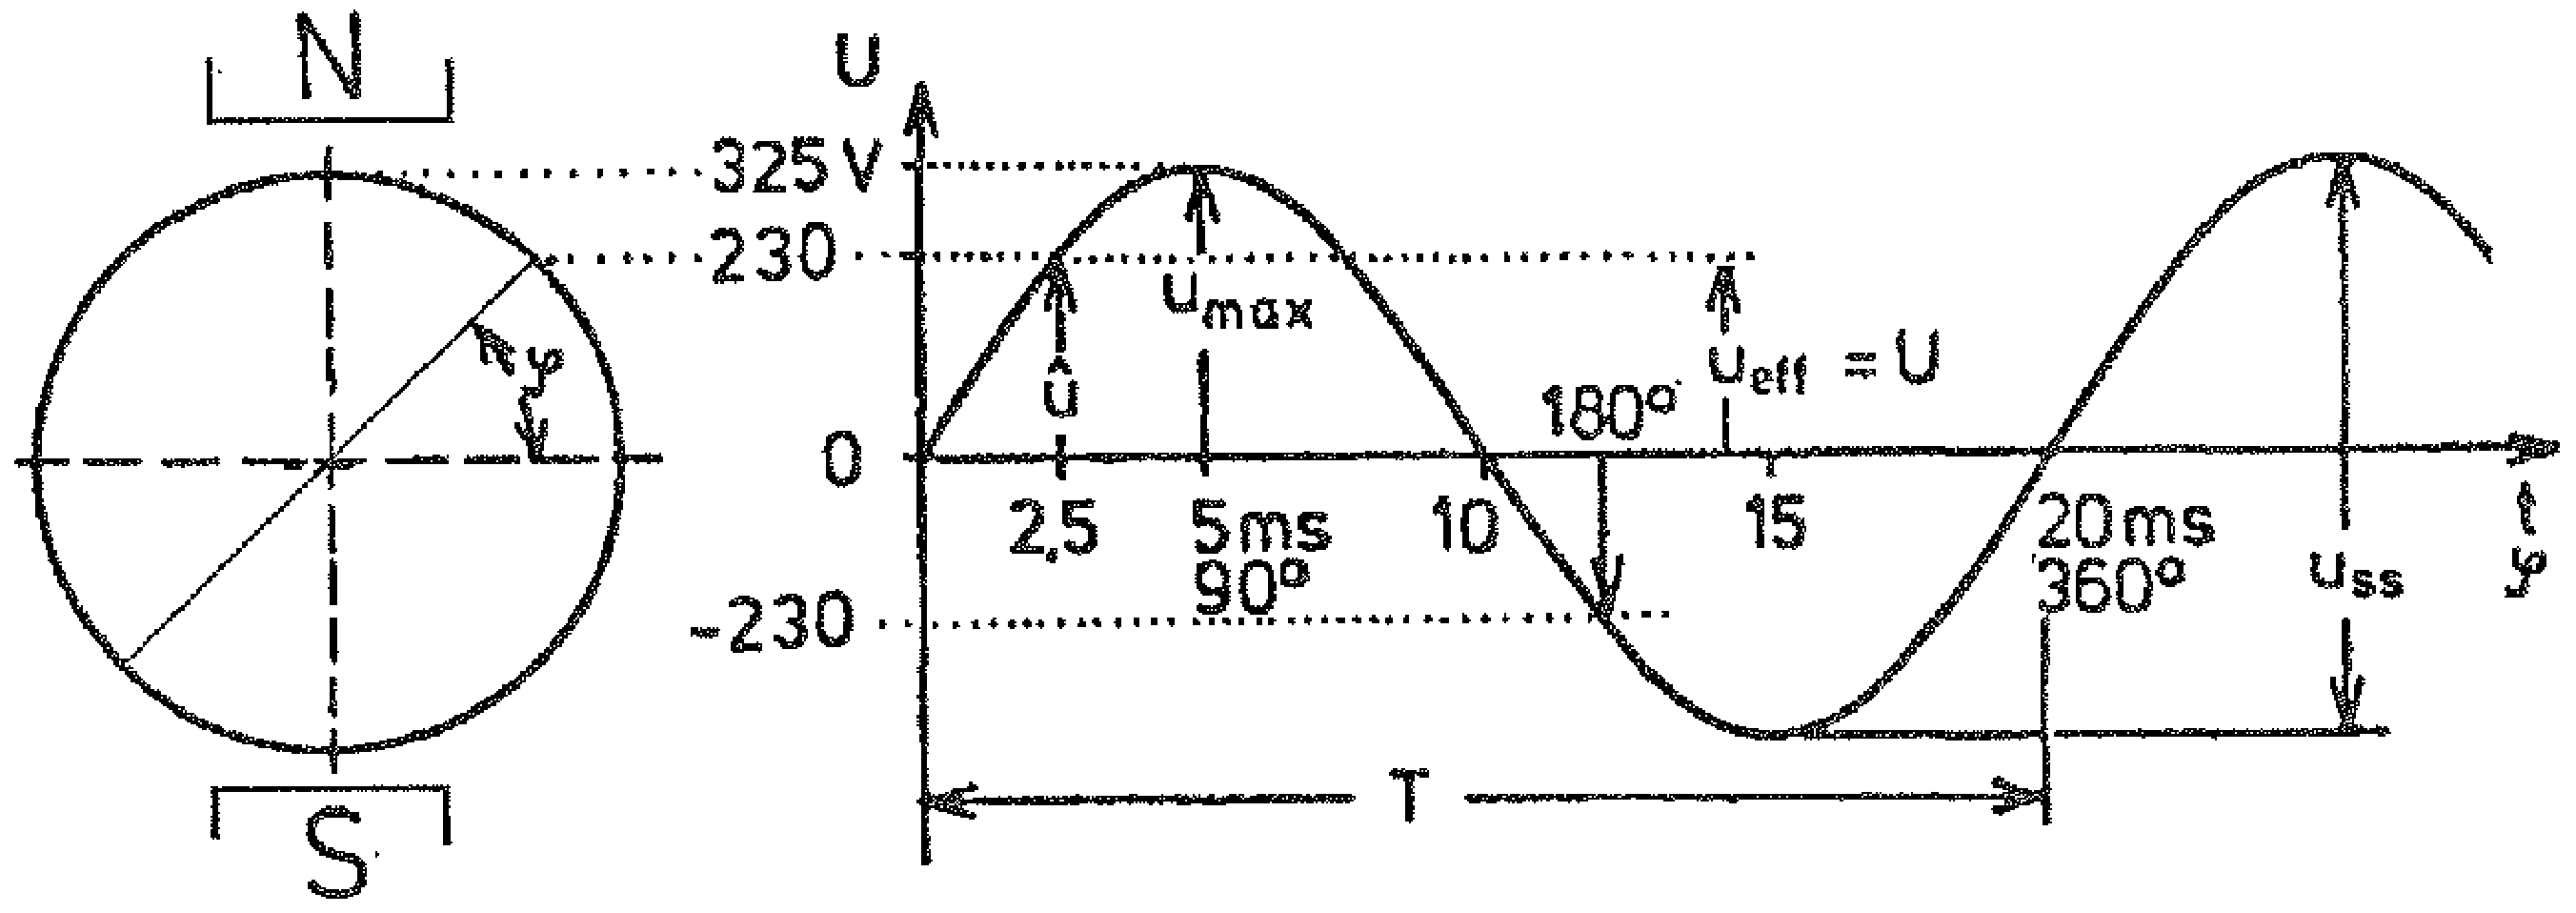
\includegraphics[width=\textwidth]{images/cropped_pdfs/bild_2_1-16.pdf}
\caption{Alstring av en sinusformad signal}
\label{fig:BildII1-16}
\end{figure}

Bild \ref{fig:BildII1-16} visar alstring av en sinusformad signal.
I detta avsnitt behandlas några grundbegrepp inom växelströmsläran.
Förloppen framställs med vektor- och linjediagram.
För närmare beskrivning används sådana begrepp som momentanvärde,
toppvärde, topp- till toppvärde, effektivvärde, fasläge, fasförskjutning och
båghastighet.

\subsection{Momentanvärde}
\textbf{HAREC a.\ref{HAREC.a.1.6.2a}\label{myHAREC.a.1.6.2a}}
\index{momentanvärde}
\index{symbol!\(u\) momentan spänning}
\index{symbol!\(i\) momentan ström}
\index{symbol!\(t\) tidpunkt}

Momentanvärdet är storheten på en spänning \(u\), en ström \(i\) etc. vid en
viss tidpunkt \(t\).
(Storheter som ändrar sig som en funktion av tiden kännetecknas ofta med gemena
bokstäver.)

Bild \ref{fig:BildII1-16} visar en sinusformad växelspänning med frekvensen
\(50\ Hz\).
Spänningen \(u\) är \(+230\ V\) vid tidpunkten 2,5~millisekunder efter en
positiv nollgenomgång.
Efter totalt \(5\, ms\) uppnås toppvärdet \(u_{max}\) d.v.s. \(+325\ V\).
Efter totalt \(10\, ms\) sker en negativ nollgenomgång.
Efter totalt \(12,5\, ms\) är spänningen \(-u\), d.v.s. \(-230\ V\) o.s.v.

\subsection{Toppvärde eller amplitud}
\textbf{HAREC a.\ref{HAREC.a.1.6.2b}\label{myHAREC.a.1.6.2b}}
\index{toppvärde}
\index{amplitud}

Toppvärdet \(u_{max}\) är det högsta värdet över eller under noll.
På bild \ref{fig:BildII1-16} är de högsta värdena \(+325\ V\) och \(-325\ V\).

\subsection{Topp-till-toppvärde}
\index{topp-till-toppvärde}

Topp-till-toppvärde är summan av toppvärdena över och under noll.
På bild \ref{fig:BildII1-16} är detta värde \(650\ V\).

\subsection{Effektivvärde}
\textbf{HAREC a.\ref{HAREC.a.1.6.2c}, a.\ref{HAREC.a.1.6.2d}\label{myHAREC.a.1.6.2c}\label{myHAREC.a.1.6.2d}}
\index{effektivvärde}

Effektivvärdet av en växelspänning \(u\) är det värde, som medför samma
effektutveckling som en likspänning \(U\).

För ett sinusformat förlopp gäller följande samband mellan toppvärdet och
effektivvärdet (det s.k. kvadratiska medelvärdet), vilket motsvarar amplituden
vid vinklarna 45, 135, 225 och 270\degree.

\(
\begin{array}{lllll}
U=\dfrac{\hat{u}}{\sqrt{2}} & & I=\dfrac{\hat{i}}{\sqrt{2}} & & (\sqrt{2} = 1,414)
\end{array}
\)

\subsection{Fasläge}
\index{fasläge}
\index{symbol!\(\phi\) fasläge}

Fasläget \(\varphi\) är när inom en period, som ett givet momentanvärde
uppträder.
Tidpunkten för varje momentanvärde motsvarar en andel av 360\degree elektriska
grader.
T.ex. uppnås värdet volt vid 0\degree, 180\degree~och 360\degree~(= 0\degree).

\subsection{Bågmått}
\index{bågmått}
\index{radianer}
\index{båghastighet (\(\omega\))}
\index{vinkelhastighet (\(\omega\))}
\index{symbol!\(\omega\) vinkelhastighet}

I beräkningar av växelströmskretsar används ofta inte vinkelmått för fasläget
(gradtal) utan i stället begreppet bågmått.

I en s.k. enhetskrets med radien \(r = 1\) motsvaras vinkeln 360\degree av en
båge med längden \(2 \cdot \pi \cdot r= 2 \cdot \pi \cdot 1 = 2 \pi =\)
omkretsen.
Vid \(f\) perioder per sekund blir båglängden \(= 2\pi f\).
Denna storhet kallas båghastigheten eller oftare vinkelhastighet och betecknas
med \(\omega\) (uttalas omega).

\(\omega= 2\pi f\) \([1/s]\)

\subsection{Period}
\textbf{HAREC a.\ref{HAREC.a.1.6.3a}\label{myHAREC.a.1.6.3a}}
\index{period}

En period har passerat, när en storhet (spänning, ström o.s.v.) återtagit samma
tillstånd eller värde efter att ha gjort en fullständig växling, t.ex. en hel
pendelrörelse eller ett helt varv vid rotation.

\subsection{Periodtid T}
\textbf{HAREC a.\ref{HAREC.a.1.6.3b}\label{myHAREC.a.1.6.3b}}
\index{periodtid (T)}
\index{symbol!\(T\) periodtid}

Periotid \(T\) är den tid som åtgår för att strömmen eller spänningen ska
genomlöpa en period. Periodtiden är det inverterade värdet av frekvensen.

Måttenheten för periodtid är sekund [s].

Periodtid

\((T) = \dfrac{1}{f}\)

\(T\ [s]  f\ [Hz]\) eller
\(T\ [ms] f\ [kHz]\) eller
\(T\ [ms] f\ [MHz]\)

Exempel:

\begin{center}
\begin{tabular}{lll}
\(T_1=\dfrac{1}{10}\) s & = 0,100 s & = 100 ms (f = 10 Hz)\\
\\
\(T_2=\dfrac{1}{50}\) s & = 0,020 s & = 20 ms (f = 50 Hz)\\
\\
\(T_3=\dfrac{1}{1000}\) s & = 0,001 s & = 1 ms (f = 1 kHz)\\
\\
\(T_4=\dfrac{1}{1000000}\) s & = 0,000001 s & = 1 \(\mu\)s (f = 1 MHz)\\
\end{tabular}
\end{center}

\subsection{Frekvens}
\textbf{HAREC a.\ref{HAREC.a.1.6.4}\label{myHAREC.a.1.6.4}}
\index{frekvens}

Frekvens är antalet perioder per tidsenhet.

Följande begrepp demonstreras med hjälp av pendeln:

Period = en fullständig fram- och tillbakasvängning i ett system, t.ex.
pendelns väg mellan punkterna 2-3-2-1-2-3- o.s.v.

\begin{figure}[ht]
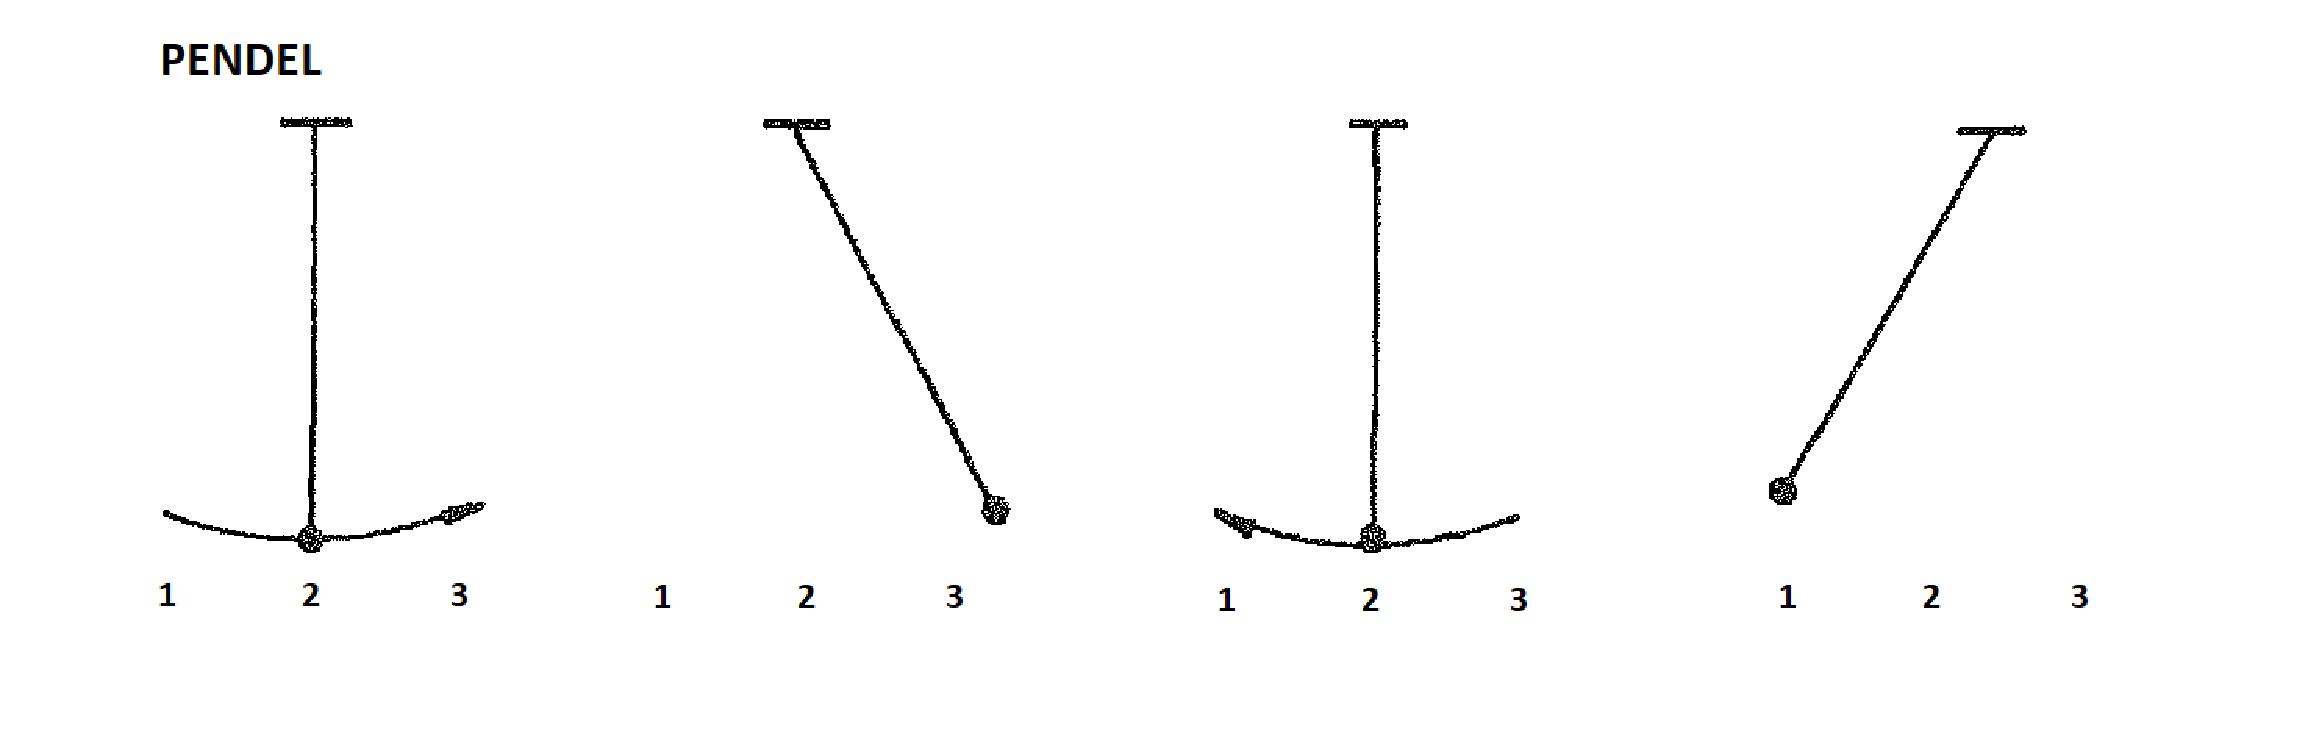
\includegraphics[width=\textwidth]{images/cropped_pdfs/bild_2_1-33.pdf}
\caption{Pendelrörelse som illustration av frekvens}
\label{fig:BildII1-33}
\end{figure}

Bild \ref{fig:BildII1-33} visar pendelrörelse som illustration av frekvens.

Periodtid \(T\) = tidsåtgången för en fullständig svängning.

Amplitud \(A\) = den största avvikelsen från viloläget.

Frekvens \(f\) = antal svängningar/tidsenhet.

Sambandet mellan frekvensen \(f\) och periodtiden \(T\) är

\(f=\dfrac{1}{T}\) t.ex.

\(5 [H z] = \dfrac{1}{5}\ [sekunder]\)

\subsection{Enheten Hertz}
\textbf{HAREC a.\ref{HAREC.a.1.6.5}\label{myHAREC.a.1.6.5}}
\index{Hertz}
\index{enheter!Hertz (Hz)}
\index{symbol!\(f\) frekvens}

Måttenheten för frekvens är Hertz [Hz].
I formler betecknas frekvensen med \(f\).

\begin{center}
\begin{tabular}{ll}
1~Hz      & = 1 period per sekund (p/s) \\
10~Hz     & = 10 perioder per sekund \\
50~Hz     & = 50 perioder per sekund \\
1~000~Hz  & = \(10^3\)~Hz = 1~kHz (kilohertz) \\
1~000~kHz & = \(10^6\)~Hz = 1~MHz (megahertz) \\
1~000~MHz & = \(10^9\)~Hz = 1~GHz (gigahertz) \\
\end{tabular}
\end{center}

Nätfrekvensen för elkraft är i Europa 50~Hz.

Andra nätfrekvenser förekommer, t.ex. 60~Hz i USA och Japan.

Frekvensområdet vid överföring av kvalitativt tal och musik, lågfrekvens LF, är
mellan ca 16~Hz och 16~kHz.

Frekvensområdet för talöverföring, t.ex. över telefonlinjer eller
kommunikationsradio, är ca 300 till 3000~Hz.

Frekvensområdet för radioöverföring, högfrekvens HF, är i huvudsak mellan
50~kHz, s.k. långvåg, och 100-tals GHz, s.k. mikrovåg.

\subsection{Fasförskjutning}
\textbf{HAREC a.\ref{HAREC.a.1.6.6}\label{myHAREC.a.1.6.6}}
\index{fasförskjutning}

\begin{figure}[ht]
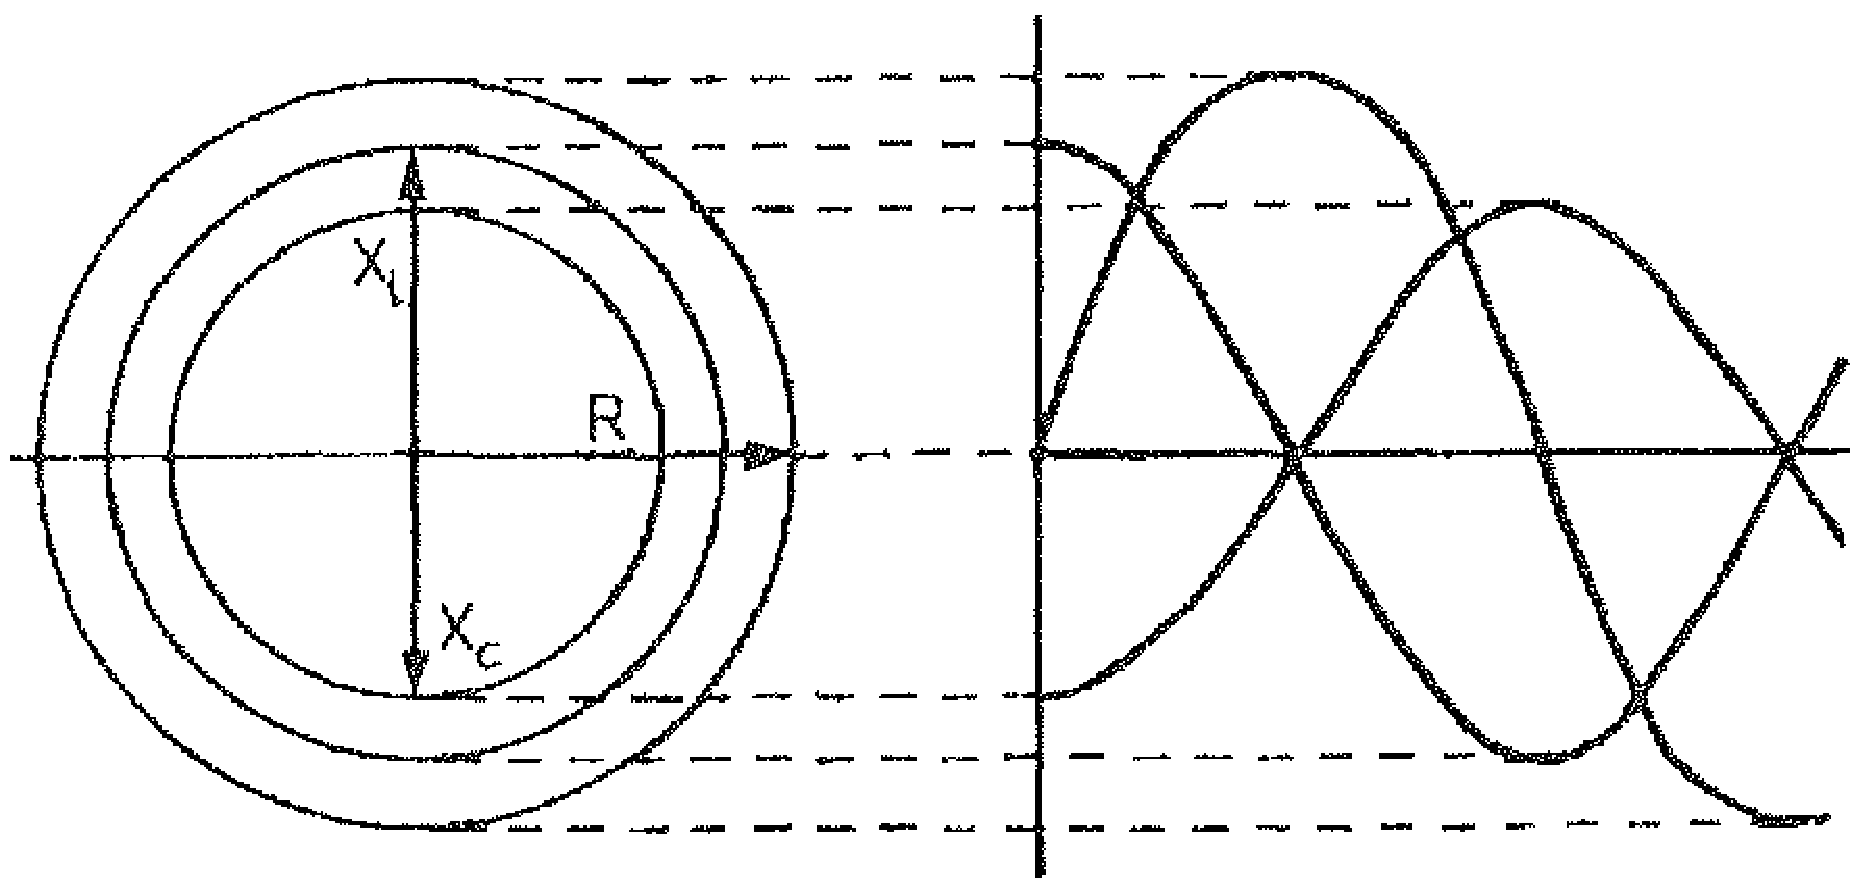
\includegraphics[width=\textwidth]{images/cropped_pdfs/bild_2_1-17.pdf}
\caption{Vektorer och fasförskjutning}
\label{fig:BildII1-17}
\end{figure}

Bild \ref{fig:BildII1-17} visar vektorer och fasförskjutning.
Med fasförskjutning menas tidsskillnaden mellan förlopp, t.ex. spänningar
och/eller strömmar.
Fasförskjutningen mellan vektorerna kallas även fasvinkel och uttrycks som ett
gradtal mellan 0 och 360\degree.

\subsection{Vektorer}
\index{vektorer}

En spänning, ström, kraft o.s.v. kan beskrivas som en vektor med en storhet och
riktning.
På bilden \ref{fig:BildII1-17} har vektorerna \(X_L\), \(R\) och \(X_C\) en
inbördes fasförskjutning av 90\degree.
De motsvarar spänningsfallen i en krets med en induktor, en resistor och en
kondensator kopplade i serie, där den gemensamma strömmen är en sinus.

Antag att vektorerna roterar i ett oförändrat inbördes läge och med en
vinkelhastighet av \(\omega= 2\pi f\).
Systemet roterar då \(360\degree = 2\pi\ radianer = 1\ varv/period\).

Vid varje tidpunkt har vektorsystemet uppnått en viss vridningsvinkel.
Momentanvärdet på vektorernas spänningar avsätts till höger i bilden.
Avståndet mellan en vektorspets och noll-linjen är vektorns momentana värde,
som kan vara positivt eller negativt.

\section{Icke sinusformade signaler}
\textbf{HAREC a.\ref{HAREC.a.1.7}\label{myHAREC.a.1.7}}

\subsection{Grundton, övertoner- Kantvågor}
\textbf{HAREC a.\ref{HAREC.a.1.7.2}, a.\ref{HAREC.a.1.7.3}, a.\ref{HAREC.a.1.7.4b}\label{myHAREC.a.1.7.2}\label{myHAREC.a.1.7.3}\label{myHAREC.a.1.7.4b}}
\index{grundton}
\index{överton}
\index{kantvåg}

\begin{figure*}
\begin{center}
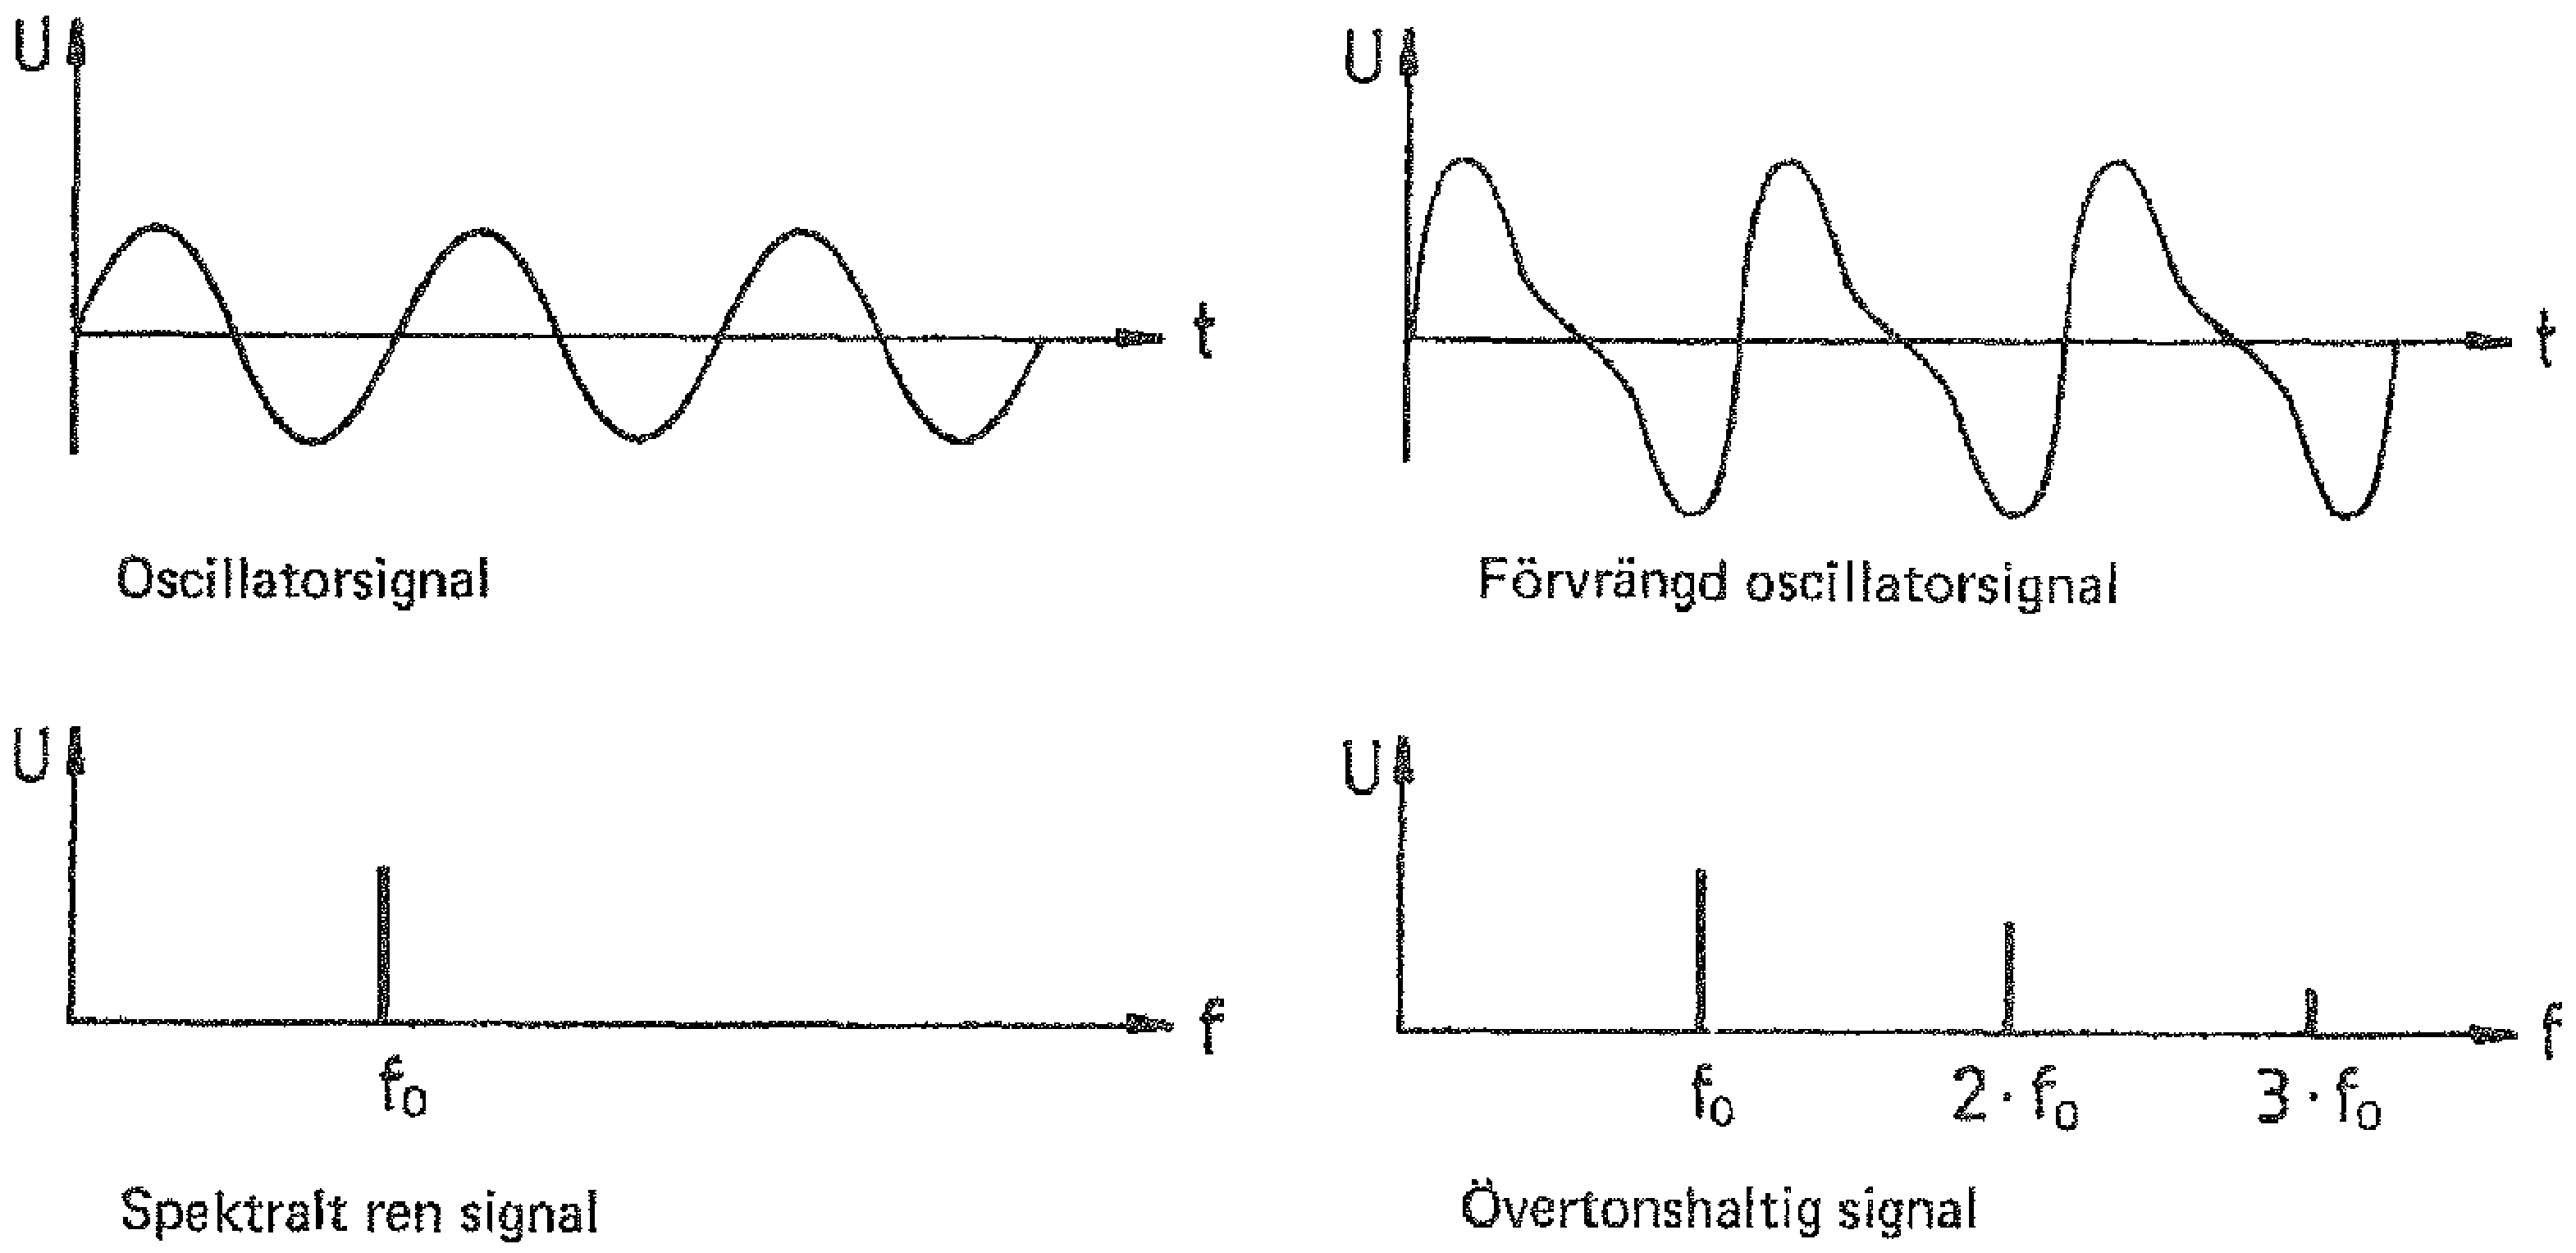
\includegraphics[width=\textwidth]{images/cropped_pdfs/bild_2_1-18.pdf}
\caption{Ren sinusvåg och övertonshaltig våg}
\label{fig:BildII1-18}
\end{center}
\end{figure*}

Bild \ref{fig:BildII1-18} visar en ren sinusvåg och övertonshaltig våg.
Ett sinusformat förlopp med en enda frekvens -- en enda ton -- sägs vara
spektralt ren.
En sådan svängning kallas för grundton.

Varje signal, som inte är sinusformad, är sammansatt av flera sinussvängningar.
Det är signalens grundton samt dess harmoniska övertoner, vilka kan ha 2, 3
o.s.v. gånger högre frekvens än grundtonen.
Den inbördes styrkan på grundton och övertoner avgör signalens form.
Om signalen ligger inom det hörbara området, kan man märka hur den ändrar
karaktär beroende på övertonshalten.
Man kan säga att övertonerna modulerar grundtonen.

\begin{figure*}
\begin{center}
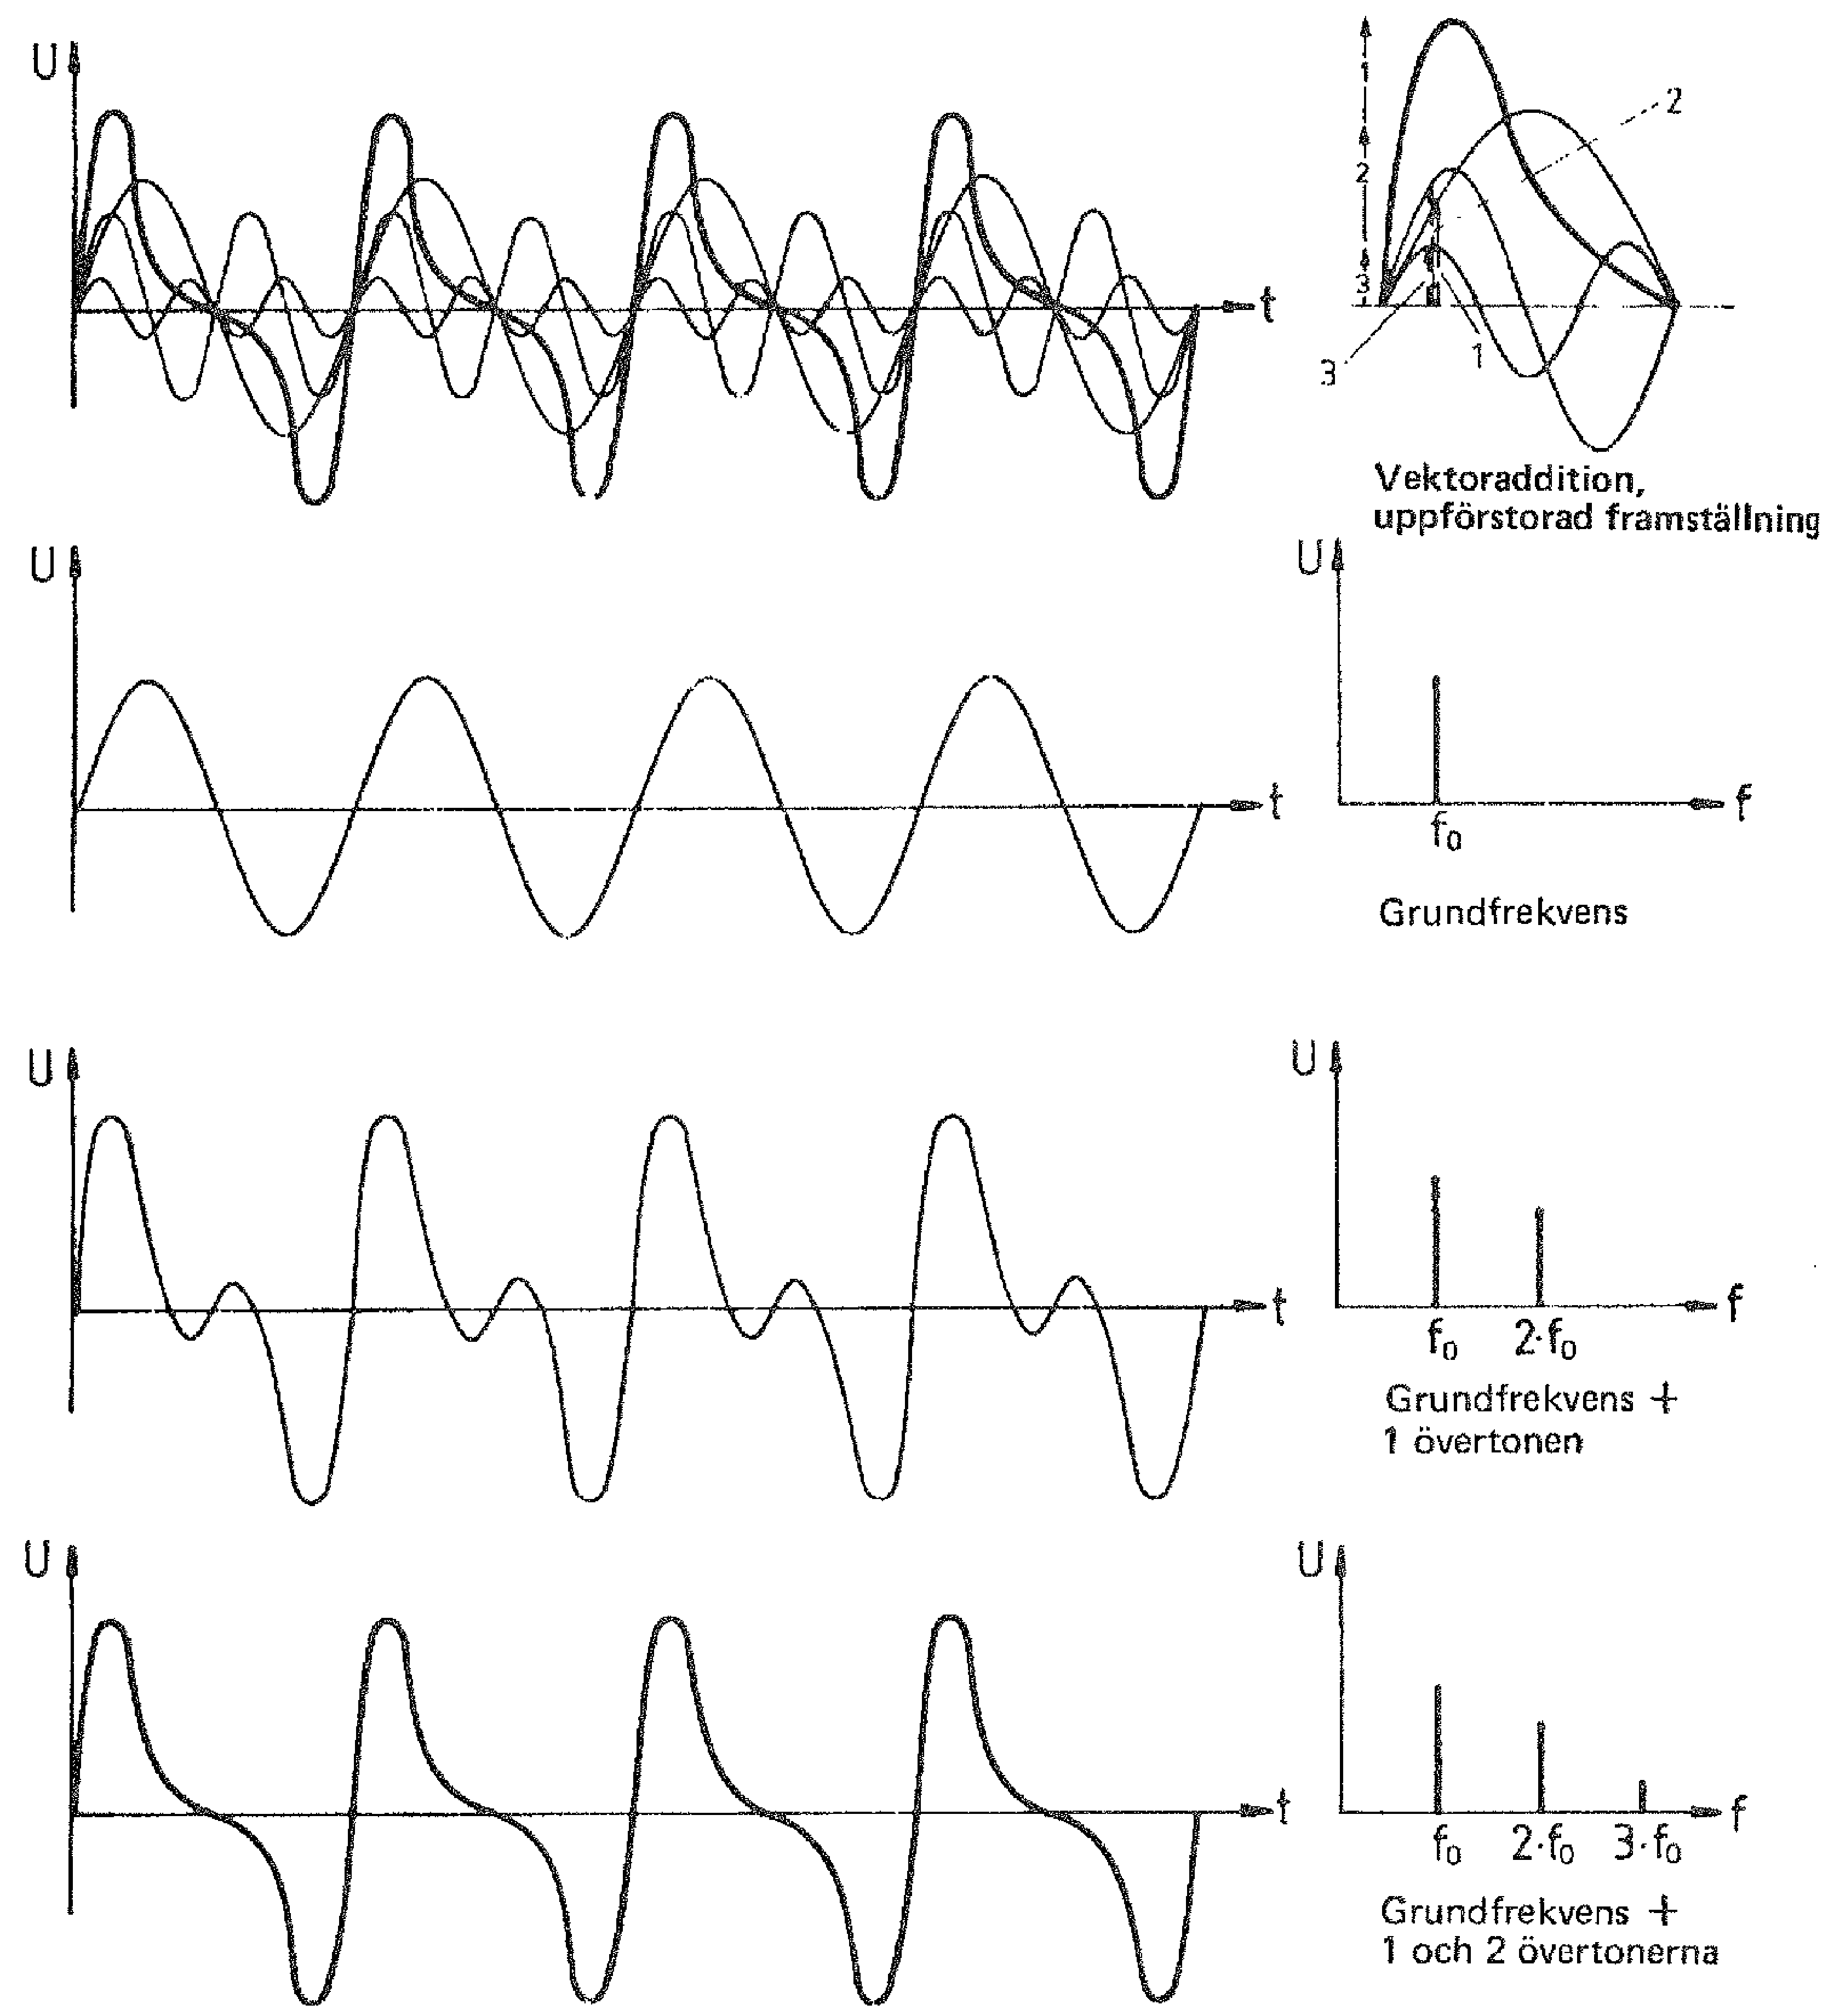
\includegraphics[width=\textwidth]{images/cropped_pdfs/bild_2_1-19.pdf}
\caption{Uppdelning av en signal i grundton och övertoner}
\label{fig:BildII1-19}
\end{center}
\end{figure*}

Bild \ref{fig:BildII1-19} visar uppdelning av en signal i grundton och
övertoner.
Oscillatorsignalen i exemplet på bilden har 1 volts amplitud på grundtonen
\(f_0\) (1:a harmoniska), 0,7~volts amplitud på de 1:a övertonen
(2:a harmoniska) och 0,2~volts amplitud på den 2:a övertonen (3:e harmoniska).
Den totala amplituden blir emellertid inte summan av 1, 0,7 och 0,2~volt
eftersom de olika delspänningarnas toppvärden inte uppträder samtidigt.
I stället måste delspänningarna adderas vid varje tidpunkt för sig.

\begin{figure*}
\begin{center}
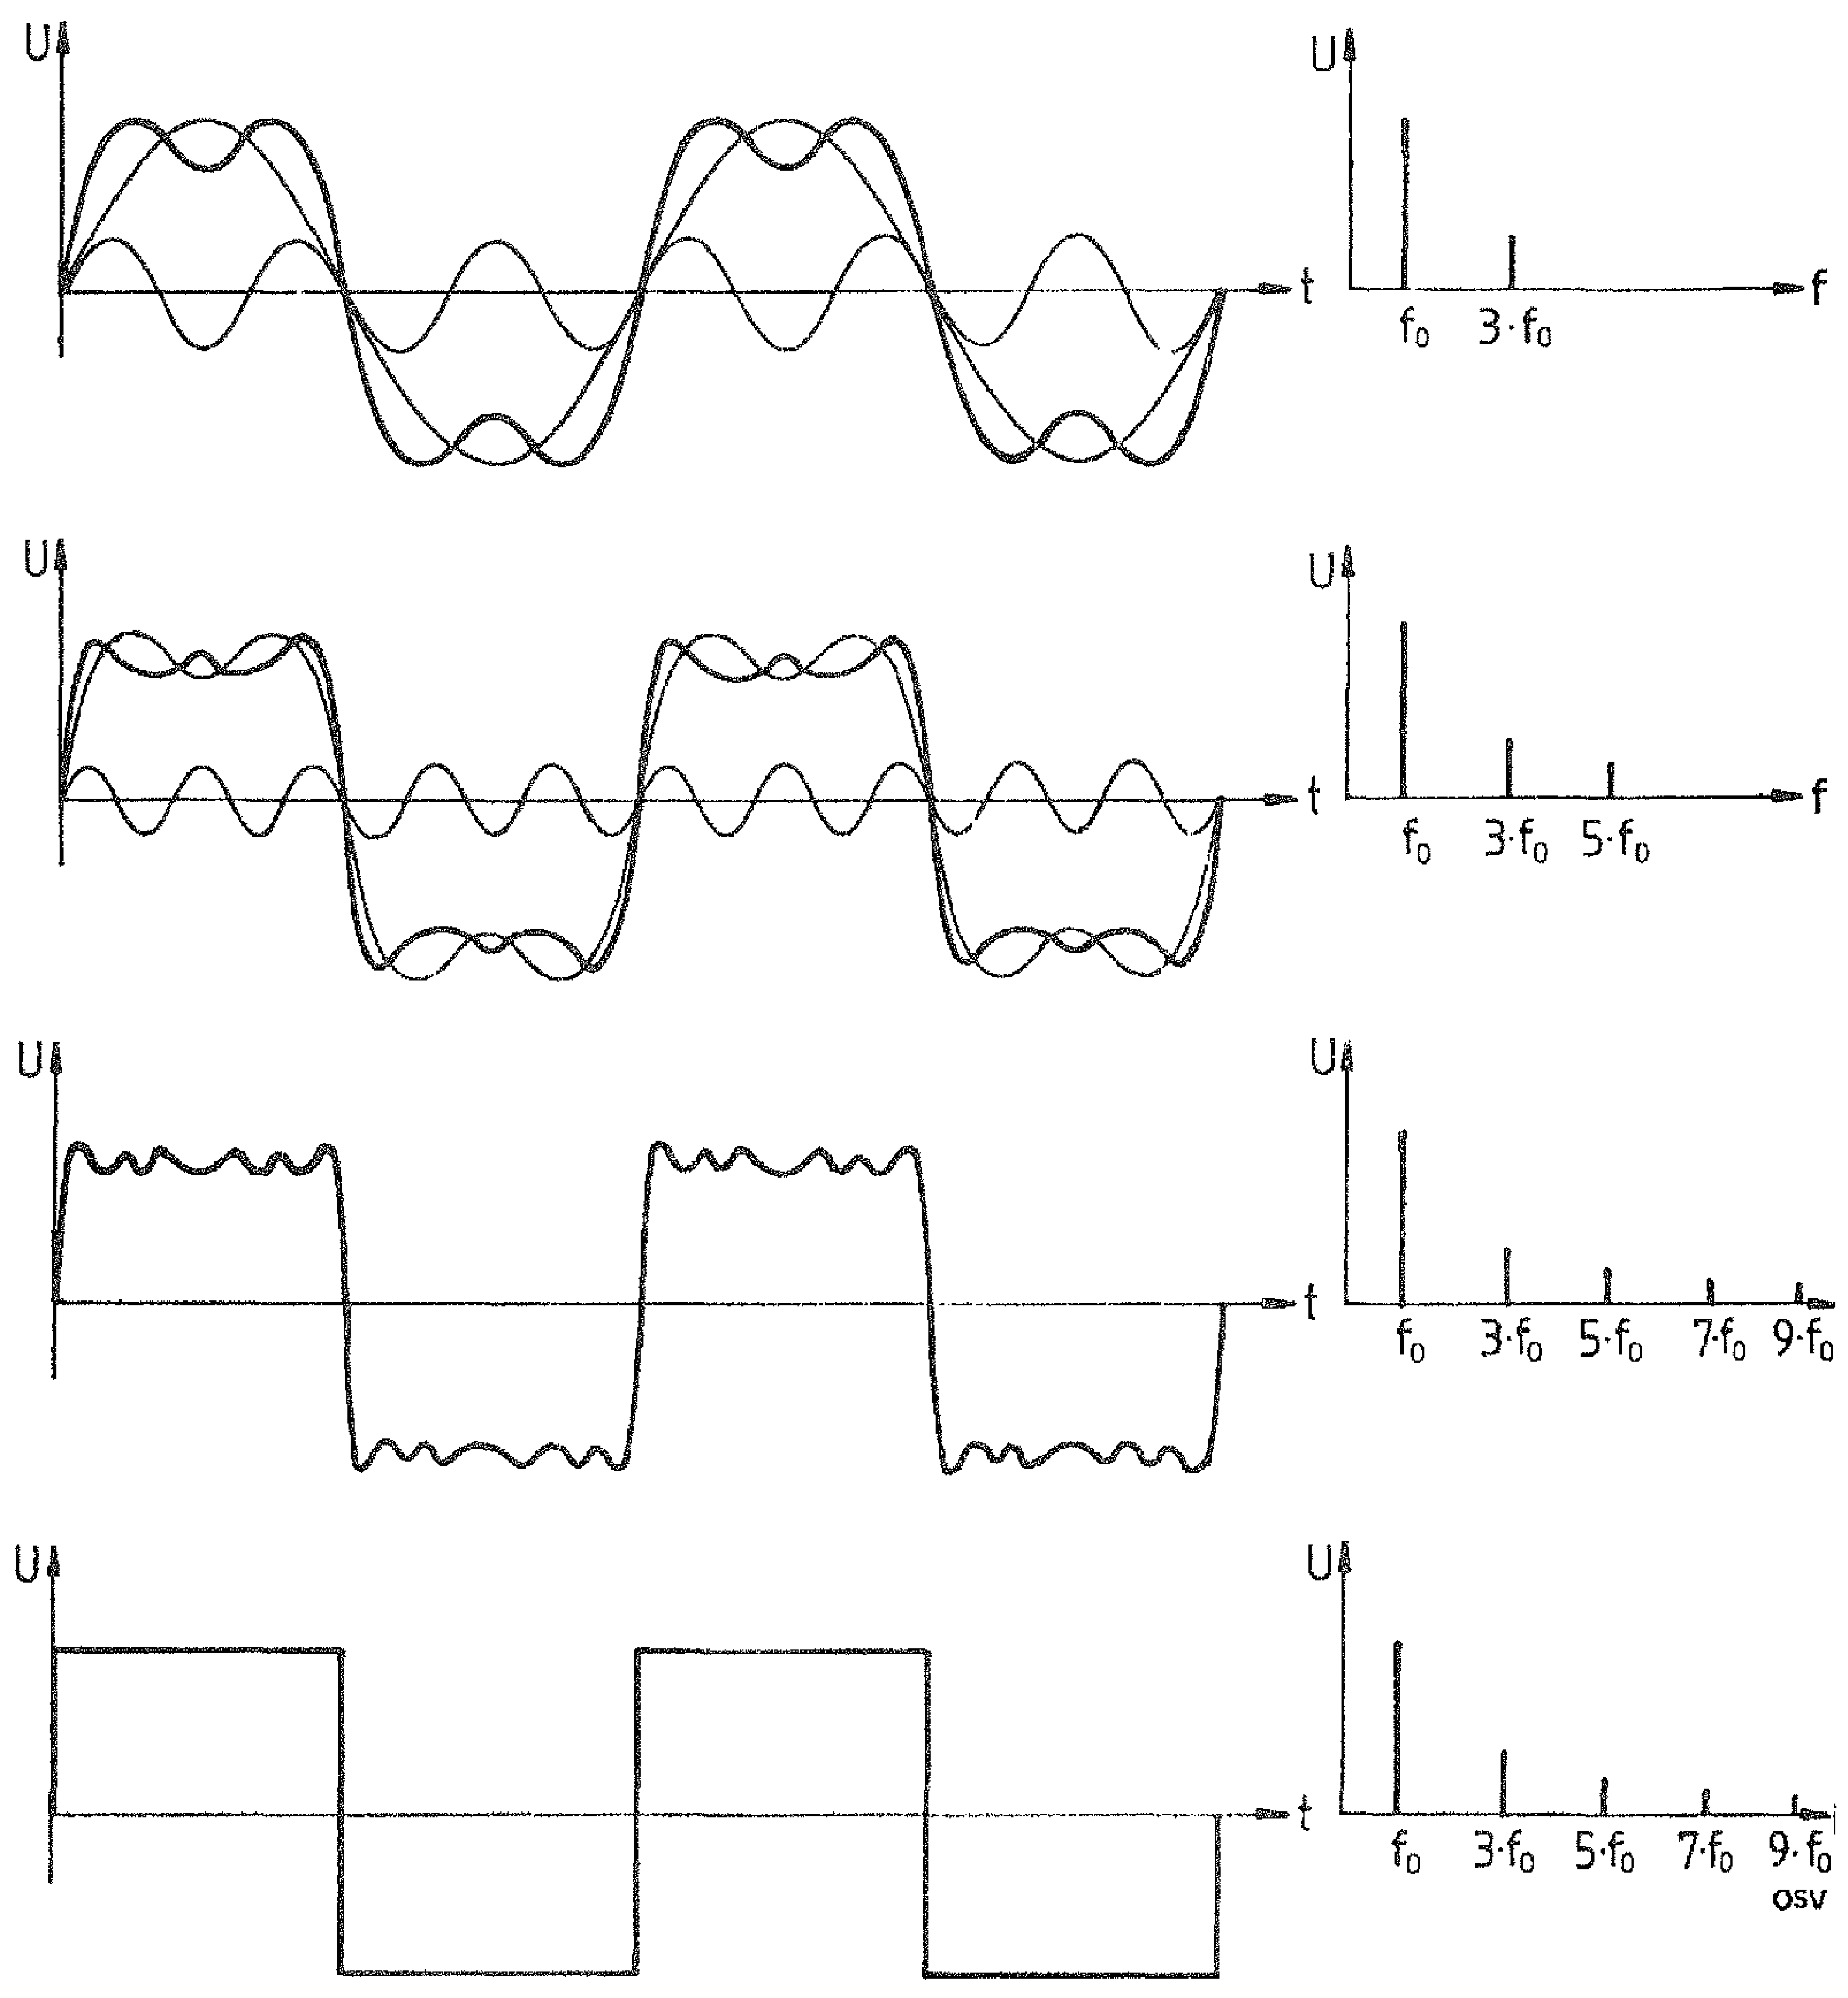
\includegraphics[width=\textwidth]{images/cropped_pdfs/bild_2_1-20.pdf}
\caption{Uppdelning av en fyrkantsvåg i grundton och övertoner}
\label{fig:BildII1-20}
\end{center}
\end{figure*}

Bild \ref{fig:BildII1-20} visar uppdelning av en fyrkantsvåg i grundton och
övertoner.

\index{Fourier, Joseph}
\index{Fourier!Fourier analys}
\index{Fourier!Fourier transform (FT)}
\index{Fourier!invers Fourier transform (IFT)}
\index{Fourier!Discrete Fourier Transform(DFT)}
\index{DFT}
\index{Fourier!inverse Discrete Fourier Transform (IDFT)}
\index{IDFT}
\index{Fourier!Fast Fourier Transform(FFT)}
\index{FFT}
\index{Fourier!inverse Fast Fourier Transform (IFFT)}
\index{IFFT}

\infobox{
Denna analys av vågor uppfanns av Jean-Baptiste Joseph Fourier (1768--1830)
vid analys av värmeutbredning och vibration som presenterades 1822.
Denna metod är kraftfull och har haft stort inflytande på vetenskapen och
utvecklingen både som matematiskt verktyg och som praktiskt analys med
spektrum-analysatorer och vid modern modulation och demodulation.
Man pratar om \emph{Fourier analys} (eng. Fourier analysis) och
\emph{Fourier transform (FT)} för omvandling från tid till frekvens och
\emph{invers Fourier transform} för omvandling från frekvens till tid.
För tidsdiskret (samplad) form är termerna
\emph{Diskret Fourier Transform (DFT)} och
\emph{invers Diskret Fourier Transform (IDFT)} respektive.
Senare optimeringar av beräkningar har resulterat i
\emph{Fast Fourier Transform (FFT)} och
\emph{Inverse Fast Fourier Transform (IFFT)}.
}

Det finns olika karaktärer av förlopp såsom sinusvåg, triangelvåg, sågtandsvåg,
fyrkantsvåg o.s.v.

Fyrkantsvågen är sammansatt av sinusvågor med grundfrekvensen och dess udda
övertoner, varvid amplituderna fördelar sig som \(1/1\), \(1/3\), \(1/5\),
\(1/7\), \(1/9\), \(1/11\) o.s.v.
Teoretiskt når övertonsspektrum upp till oändligt höga frekvenser, medan de
motsvarande amplituderna minskar till oändligt små värden.

En ideal fyrkantsvåg, vilken inte kan uppnås i praktiken, skulle bestå av ett
oändligt antal udda övertoner med fallande amplitud.
Ju fler av de högre övertonerna som filtreras bort, desto mer lutar
fyrkantsvågens flanker, desto rundare blir hörnen på vågen och desto vågigare
blir kurvans topp.

\subsection{Överlagrade spänningar
(likspänningskomposant)}
\textbf{HAREC a.\ref{HAREC.a.1.7.4a}\label{myHAREC.a.1.7.4a}}

\begin{figure}[ht]
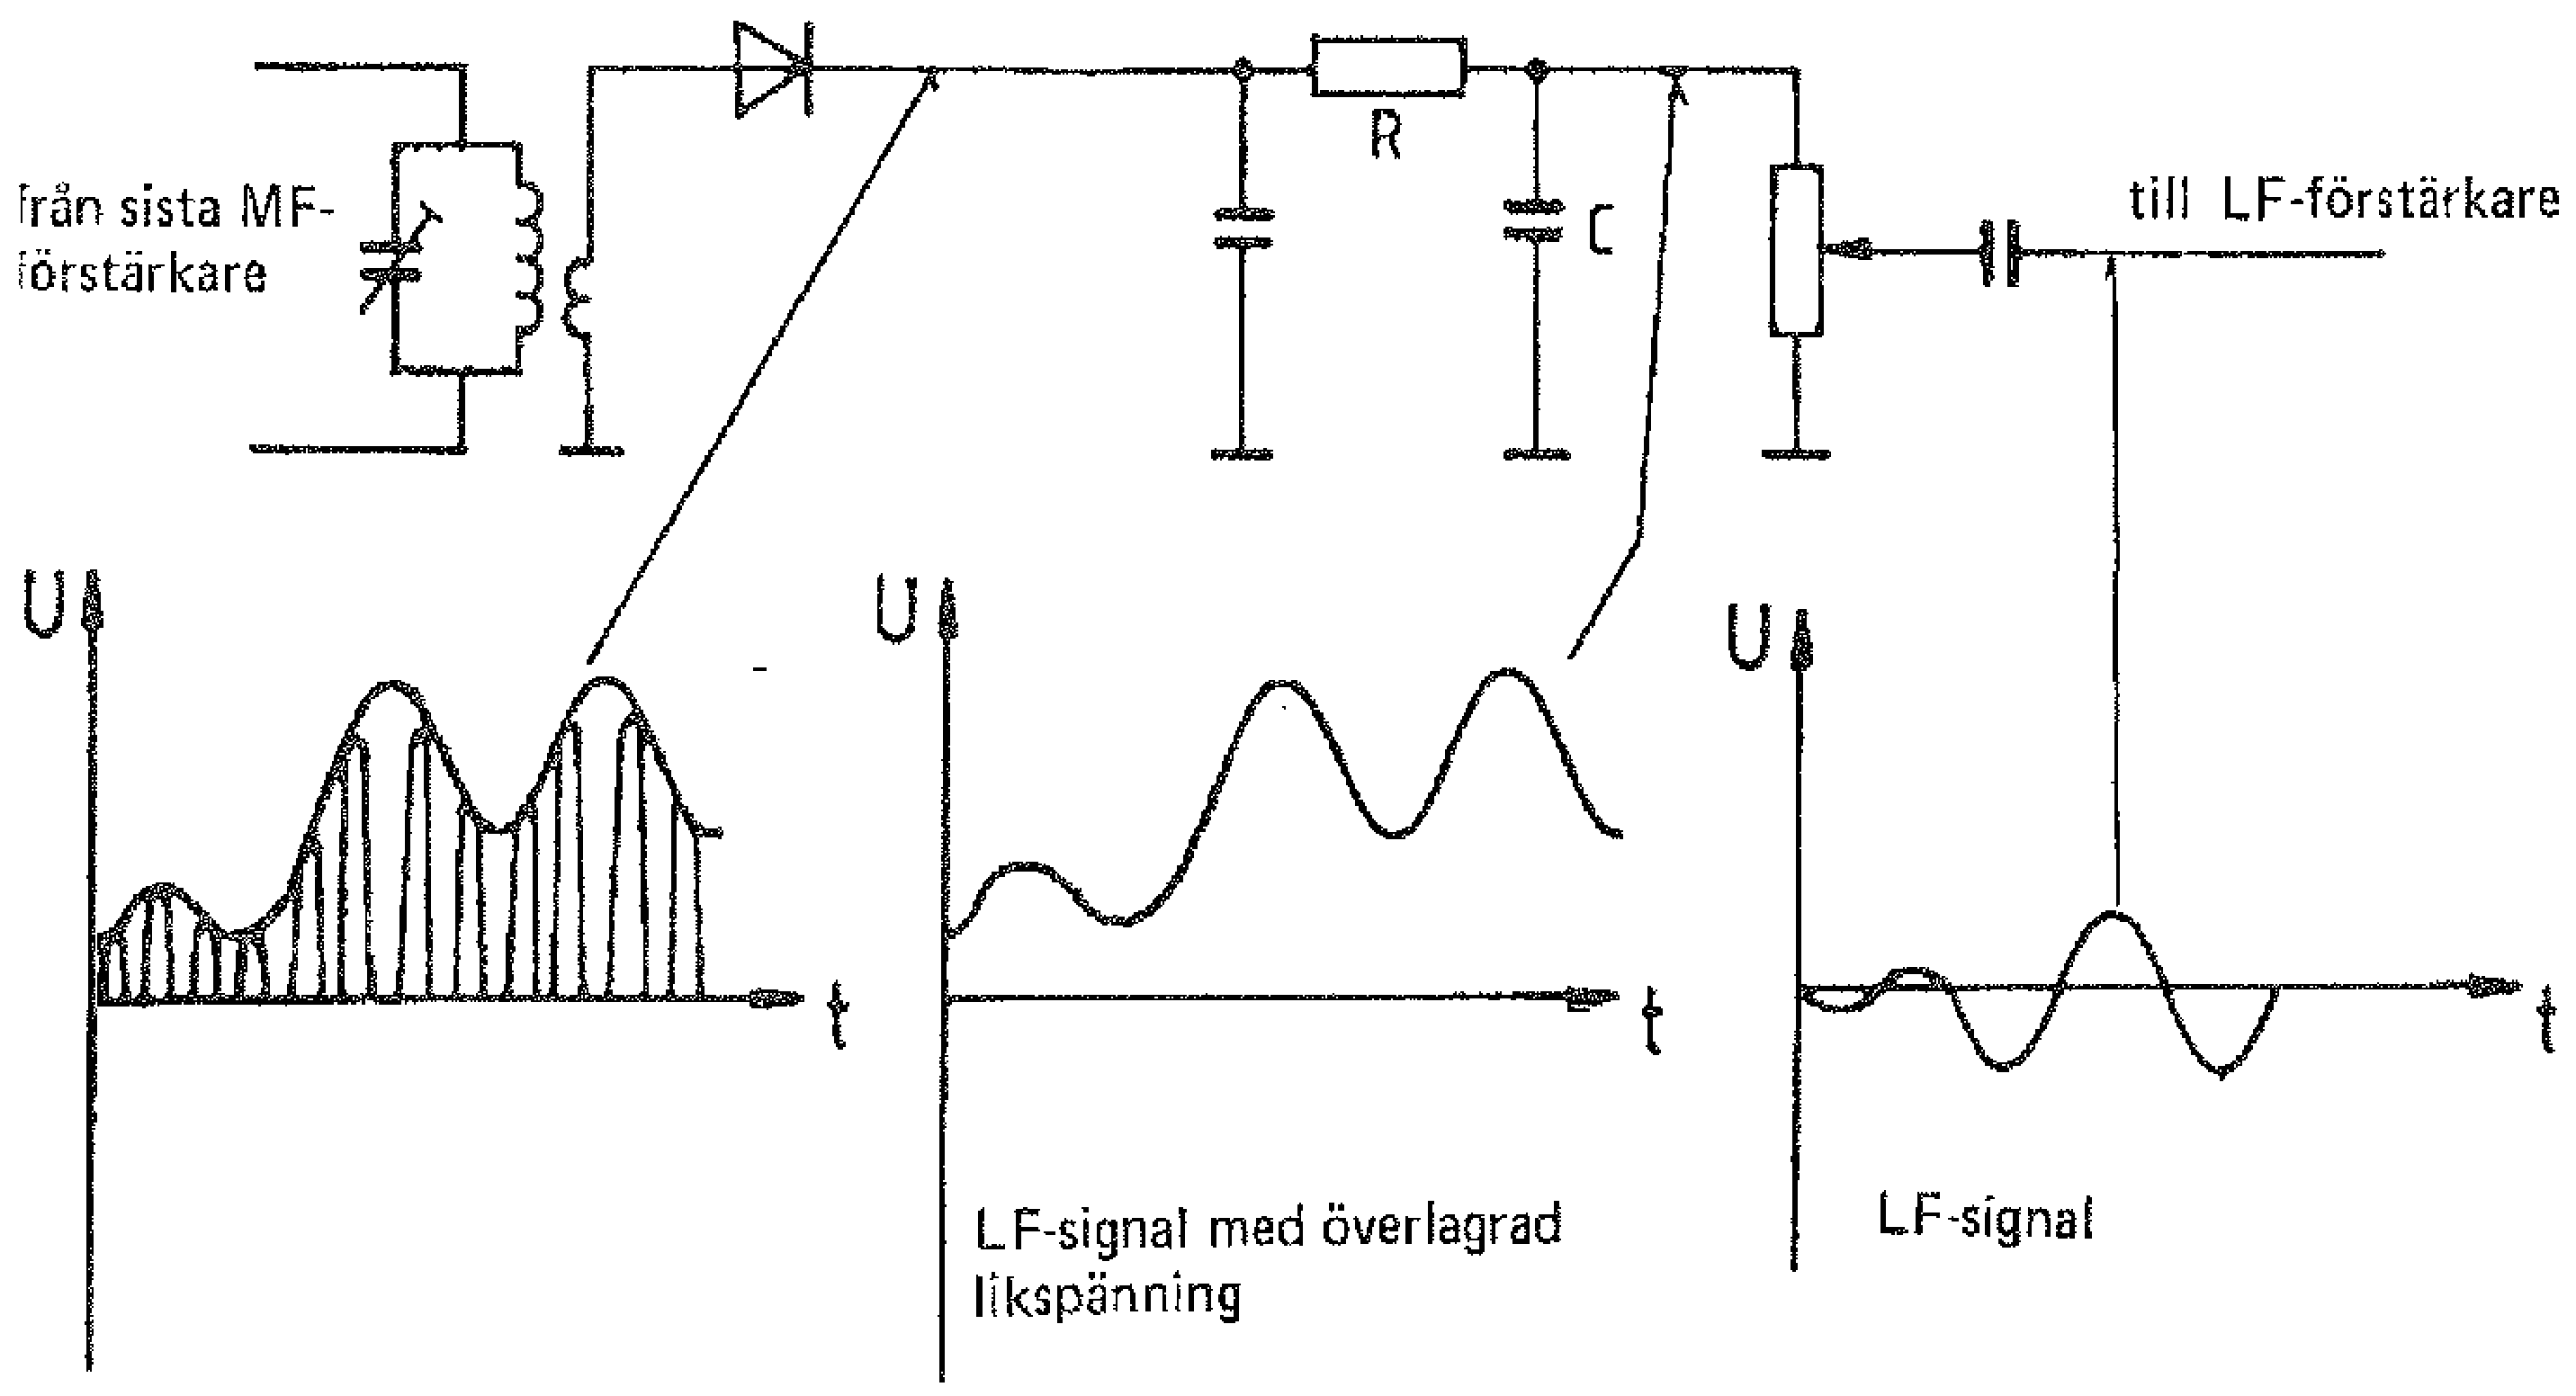
\includegraphics[width=\textwidth]{images/cropped_pdfs/bild_2_1-21.pdf}
\caption{Överlagrade spänningar}
\label{fig:BildII1-21}
\end{figure}

Bild \ref{fig:BildII1-21} visar överlagrade spänningar.
I signalkretsar förekommer det mycket ofta, att växelspänning överlagras på
likspänning eller omvänt.
Likspänningen kallas då för likspänningskomposant.
Olika åtgärder behövs för att överlagra spänningar på varandra och att sedan
skilja dem åt.

Bilden visar ett avsnitt av en AM-mottagare.
Från vänster hämtas en AM-modulerad signal från MF-förstärkaren för att
demoduleras, d.v.s. för att återvinna den modulerande LF-signalen.
MF-signalen halvvågslikriktas.
Kvar blir den positiva delen av MF-signalen och den modulerande LF-signalen,
sammanlagrade.
LF-signalen ska nu skiljas ut och förstärkas.
Alltså filtreras MF-komposanten bort.
Kvar blir LF-signalen, men överlagrad på en likspänning.
Likspänningen stoppas och kvar blir slutligen LF-signalen som förstärks.

\subsection{Brus}
\textbf{HAREC a.\ref{HAREC.a.1.7.5}\label{myHAREC.a.1.7.5}, a.\ref{HAREC.a.7.19}\label{myHAREC.a.7.19}}
\label{termisktbrus}

\subsubsection{Termiskt brus}
\index{brus}
\index{termiskt brus}
\index{brus!termiskt}

Resistorer och resistans, i alla dess former, uppvisar en egenskap av
en varierande spänning även när ingen ström går genom motståndet.
Denna extra spänning innehåller ett brett spektra av toner, men är också ett
tätt spektra, sådan att ingen enskild ton kan särskiljas från någon annan.
Istället för att tänka sig en grundton och dess övertoner med ingen energi
emellan dem så är det istället ett kontinuerligt spektra med oändligt många
toner.
Detta spektra begränsas dock av bandbredden.

\begin{wrapfigure}{R}{0.5\textwidth}
  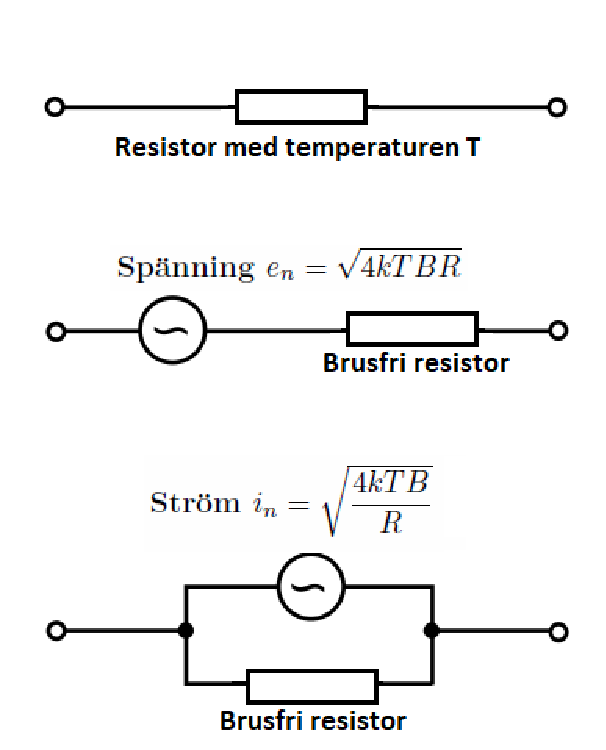
\includegraphics[width=0.5\textwidth]{images/cropped_pdfs/bild_2_1-36.pdf}
  \caption{En resistor kan ses ha brus ekvivalenter som spänning eller ström}
  \label{fig:BildII1-36}
\end{wrapfigure}

\begin{wrapfigure}{R}{0.5\textwidth}
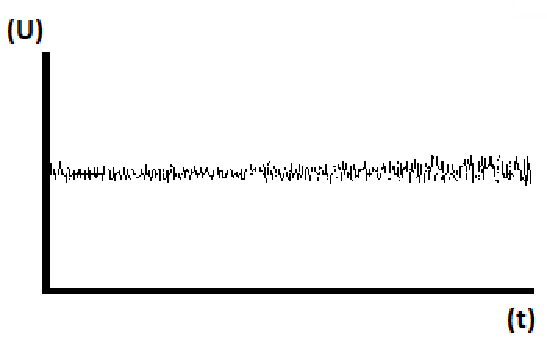
\includegraphics[width=0.5\textwidth]{images/cropped_pdfs/bild_2_1-34.pdf}
\caption{Brus innebär en ostabilitet över tid}
\label{fig:BildII1-34}
\end{wrapfigure}

\begin{wrapfigure}{R}{0.5\textwidth}
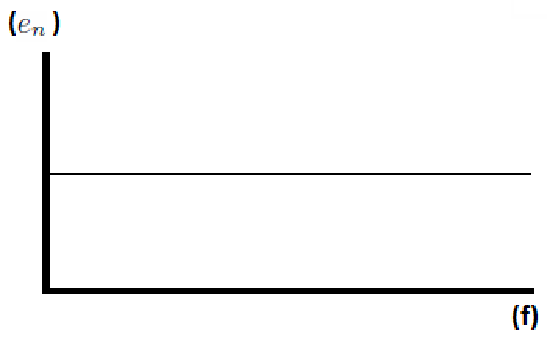
\includegraphics[width=0.5\textwidth]{images/cropped_pdfs/bild_2_1-35.pdf}
\caption{Brus innehåller alla frekvenser, vitt brus har samma amplitud}
\label{fig:BildII1-35}
\end{wrapfigure}

\index{vitt brus}
\index{brus!vitt}
\index{white noise}
\index{Johnsson noise}
\index{brus!Johnsson}
Man kallar detta spektra i daglig tal för \emph{termiskt brus}
(eng. thermal noise), eftersom det beror på temperaturen hos motståndet, eller
\emph{Johnsson noise}, efter J. B. Johnsson som 1928 fann att detta brus fanns
i alla ledare \cite{ott1988}.
Brus skapar en variation i spänning och ström, som illustreras i bild
\ref{fig:BildII1-34}.

I dagligt tal pratar man dock bara om \emph{vitt brus} (eng. white noise) eller
\emph{brus}.
Med vitt brus menas brus som inte ''färgats'', och det betyder i det här
sammanhanget att det har samma amplitud för alla frekvenser, så som illustreras
i bild \ref{fig:BildII1-35}.
I praktiken är allt brus begränsat med bandbredden på kanalen, men man
betraktar det som vitt inom kanalen om det är jämn inom bandet.

Effekten \(P_n\) av detta brus beror på Boltzmanns konstant
\(k\ =\ 1,38 \cdot 10^{-23}\) J/K, den absoluta temperaturen \(T\) i
kelvin samt bandbredden \(B\) i hertz och anges enligt formeln:

\(P_n = k T B\)

Varje motstånd med den absoluta temperaturen T kan modelleras som att ha en
ekvivalent spänning \(e_n\) och ström \(i_n\) för resistansen \(R\),
så som illustreras i bild \ref{fig:BildII1-36} är

\(e_n = \sqrt{4kTBR}\)

\(i_n = \sqrt{\dfrac{4kTB}{R}}\)

\subsubsection{Brusbandbredd}
\index{brus!brusbandbredd}

Medans vi initialt antagit att brusets bandbredd är för frekvenser
från DC till övre gränsfrekvensen så är det inte nödvändigt.
Formeln är även relevant för bruset på ett band, och bandbredden för det
bandpass filter vi har för att enbart lyssna på detta band.

Exempelvis behöver tal på SSB hantera 300~Hz till 3~kHz, dvs. 2,7~kHz
bandbredd och därmed kommer även mottagarens bandbredd behöva vara så stort,
och därmed även brusbandbredd på 2,7~kHz.
Vi kommer då att ta emot brus för motsvarande bandbredd.
Ett CW filter kan t.ex. vara 350~Hz och kommer därmed också ha ett
motsvarande förhållande lägre brus-effekt.

Detta är dock en förenkling, eftersom filtret inte filtrerar med branta kanter
och är helt plant.
Filtrets egentliga brus-bandbredd beror på hur filtret filtrerar över
alla frekvenser och summan av dessa.
Beroende på vilken typ av filter så behövs därför en korrigeringsfaktor
från den normala bandbredden till brus-bandbredden.
För ett normalt 12~dB/oktav lågpassfilter är korrigeringsfaktorn 1,22.

\section{Modulation}
\textbf{HAREC a.\ref{HAREC.a.1.8}\label{myHAREC.a.1.8}}
\label{modulation}
\index{modulation}

\subsection{Allmänt}

\emph{Modulera} (lat. \emph{modulari}, rytmiskt avmäta) är att med hjälp av en
oftast högfrekvent elektrisk signal (bärvågen) överföra informationen i en
lågfrekvent signal. På så sätt kan lågfrekvens, t.ex. tal och musik, först
omvandlas till en elektrisk signal, som får påverka (modulera) en högfrekvent
elektrisk signal. Denna modulerade signal strålas ut från antennen som ett
elektromagnetiskt fält.

Den signal som innehåller informationen kallas \emph{modulerande signal} eller
\emph{basband} eller \emph{underbärvåg}.

Den signal som informationen överförts till kallas \emph{modulerad signal}
eller \emph{huvudbärvåg}.

\subsection{Modulationssystem}

Den största gruppen av modulationssystem är definierad med avseende på hur
huvudbärvågen är modulerad. Vanligast är då amplitud- och vinkel modulation.
Av vinkelmodulation finns främst två slag, frekvensmodulation och
fasmodulation. Därutöver finns system för pulsmodulation.

\subsection{Sändningsslag}
\index{sändningsslag}

Sätten att modulera kallas \emph{sändningsslag}. Gemensamt för sändningsslagen
är att en givare -- det kan vara en mikrofon, en telegrafnyckel, en
fjärrskriftsmaskin, en dator, en TV-kamera o.s.v. -- alstrar en analog eller
digital signal. Denna styr underbärvågen så att huvudbärvågen moduleras med den
avsedda informationen och sänds ut.

Det enklaste sändningsslaget får anses vara morsetelegrafi med ''nycklad bärvåg''.
Då förekommer bara två tillstånd, nedtryckt och icke nedtryckt telegrafnyckel,
d.v.s. antingen bärvåg med någon varaktighet eller ingen bärvåg alls.
Kombinationer av bärvågselement med olika längd motsvarar skrivtecken.

För att återge tal, musik etc. behövs en noggrannare tillståndsstyrning av
bärvågen. Det innebär att bärvågen måste moduleras av en underbärvåg och att
denna motsvarar lufttrycksvariationerna i ljudet.

\subsection{Kännetecken för modulerade signaler}
\textbf{HAREC a.\ref{HAREC.a.1.8.5}\label{myHAREC.a.1.8.5a}}

\begin{figure}
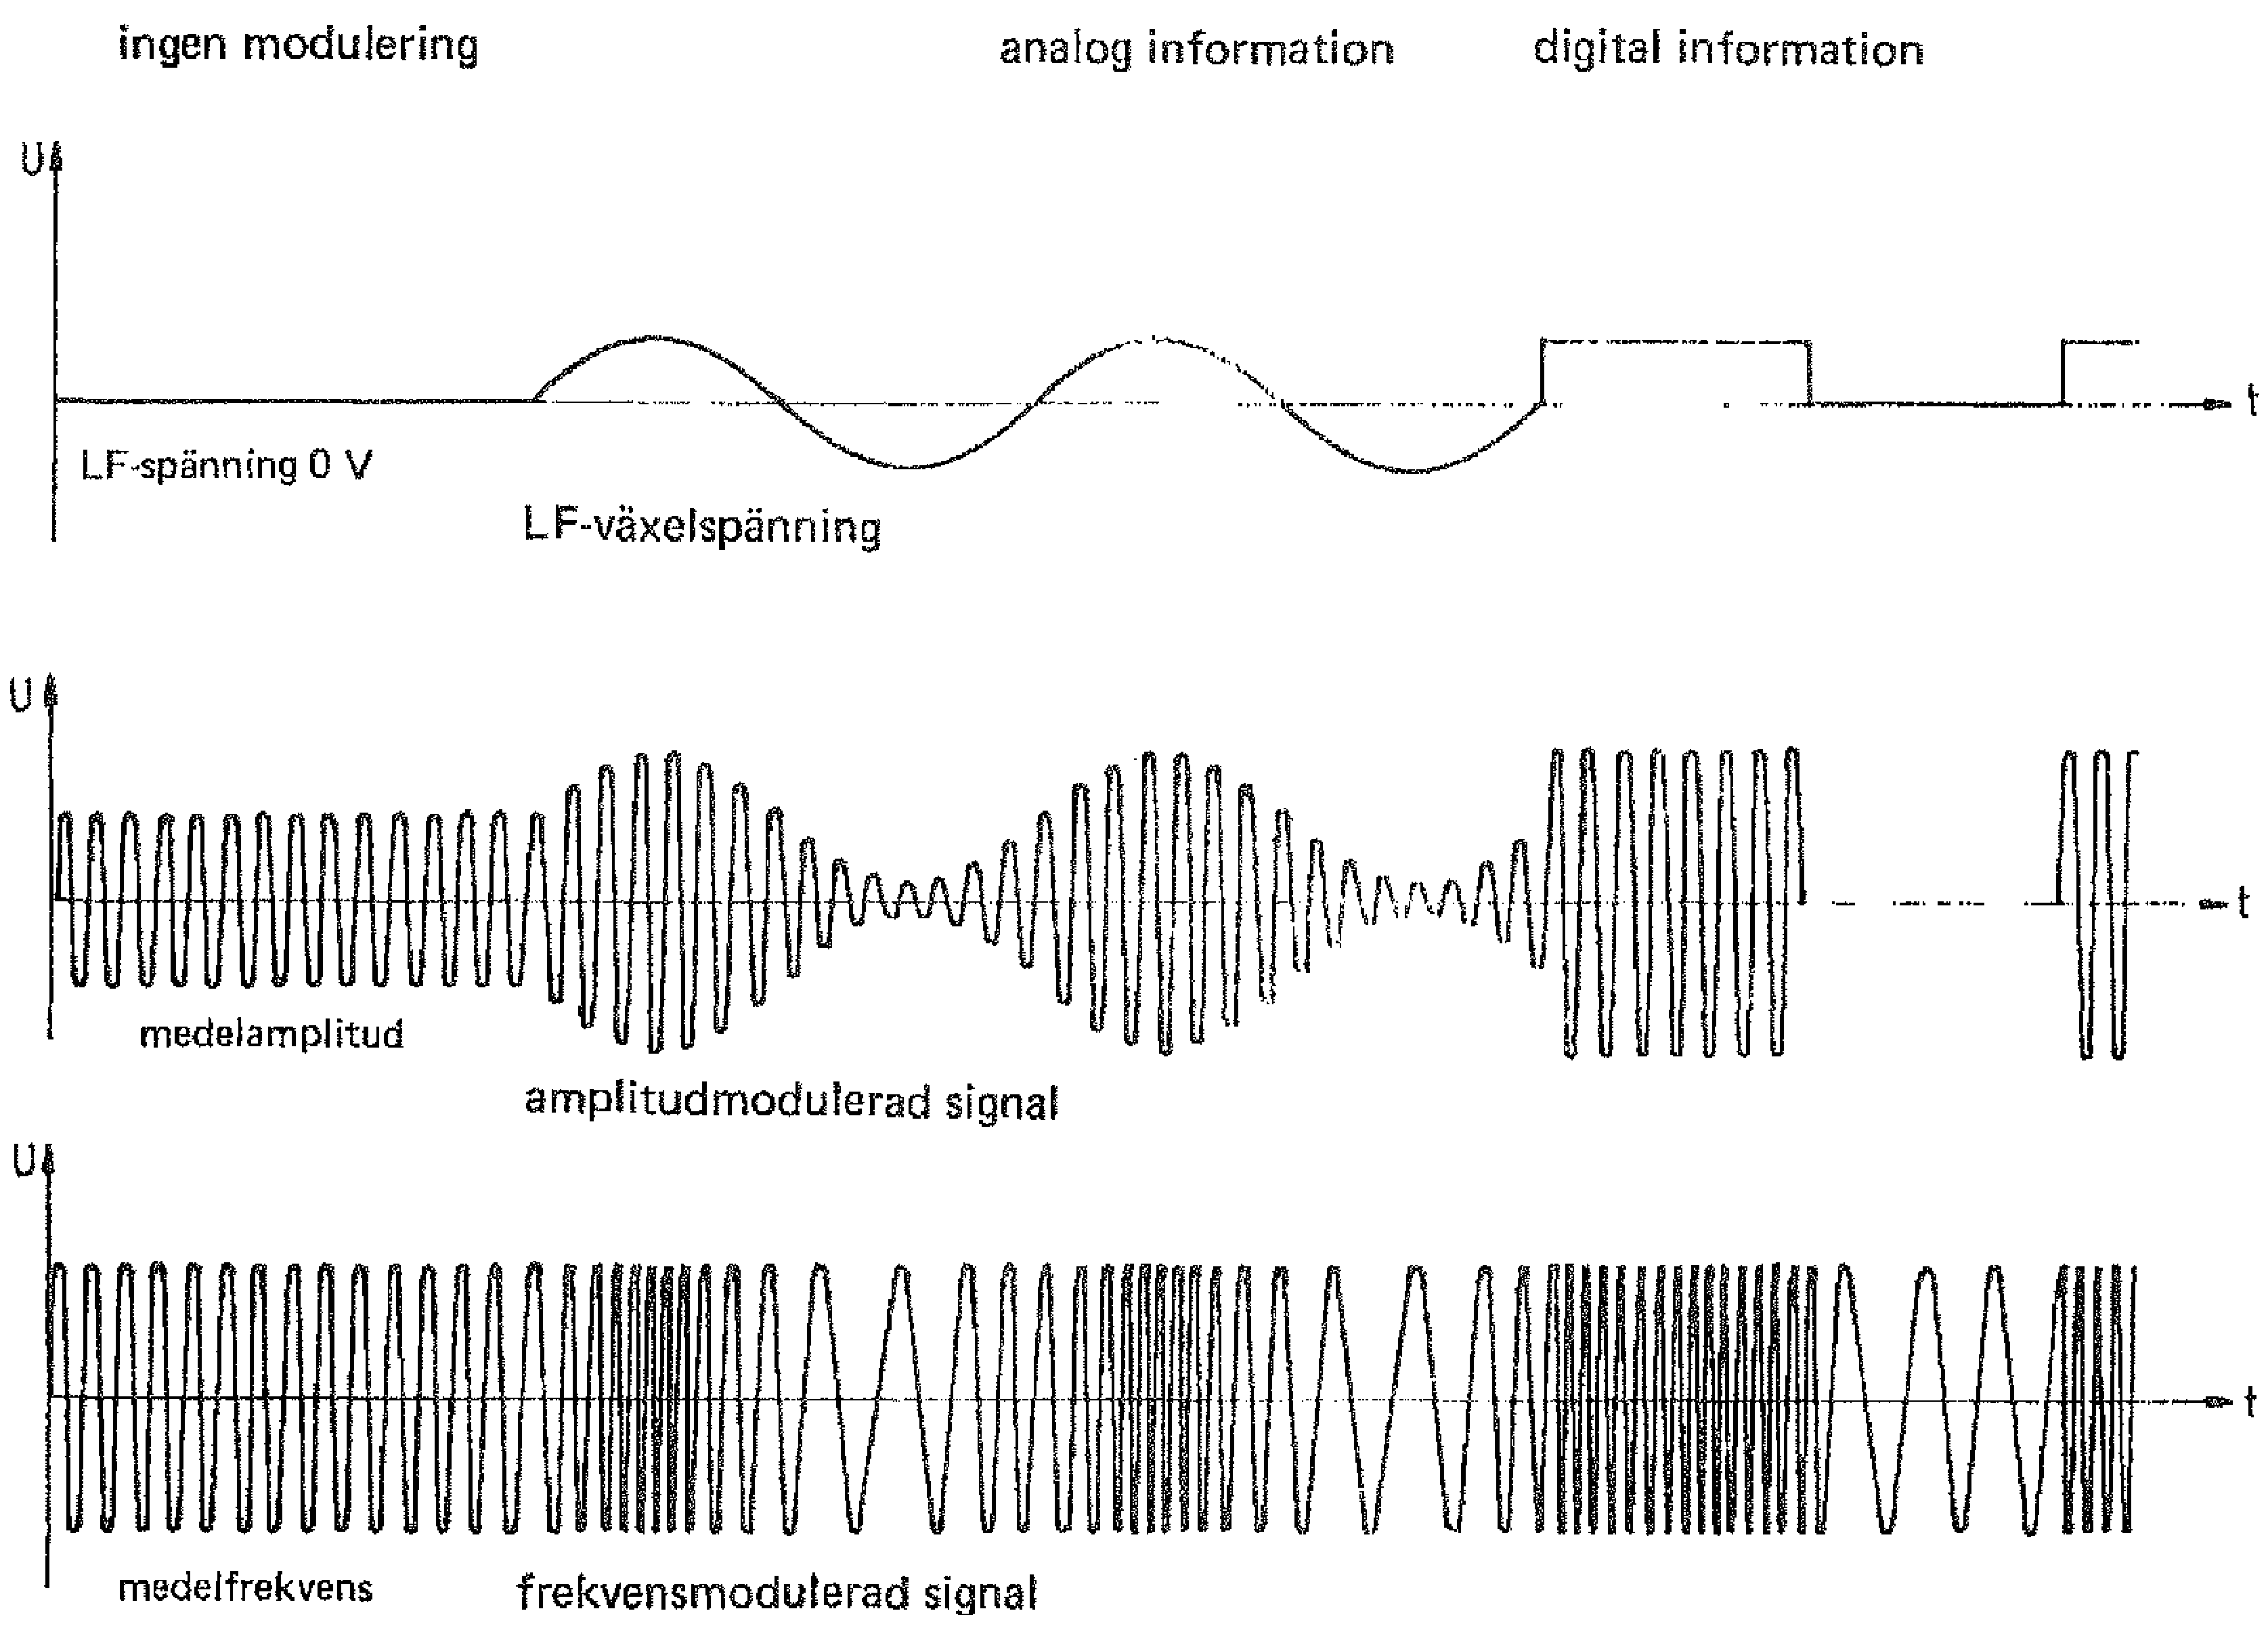
\includegraphics[width=\textwidth]{images/cropped_pdfs/bild_2_1-22.pdf}
\caption{Modulerade signaler}
\label{fig:BildII1-22}
\end{figure}

Bild \ref{fig:BildII1-22}.

En modulerad signal kännetecknas av dess amplitud, frekvens och fasläge.

Vid \emph{amplitudmodulation} påverkas huvudbärvågens amplitud, så att den i
varje tidpunkt motsvarar den modulerande signalens variation.

Vid \emph{frekvensmodulation} påverkas huvudbärvågens frekvens, så att den i
varje tidpunkt motsvarar den modulerande signalens variation.

Vid \emph{fasmodulation}, som är besläktad med frekvensmodulation, påverkas i
stället för frekvensen huvudbärvågens fasläge i förhållande till en
referenssignal, så att fasläget i varje tidpunkt motsvarar den modulerande
signalens variation.

Frekvens- och fasmodulation liknar varandra och kan sammanfattas som
vinkelmodulation, eftersom fasvinkeln mellan bärvågens spänning och ström
varierar i båda fallen.

Vid \emph{pulsmodulation} används pulståg (korta upprepade bärvågspaket); t.ex.
pulsamplitud-, pulslängds-, pulsläges- och pulskodmodulation. Pulskodmodulation
används t.ex. vid samtidig överföring av flera telesamtal på samma linje,
bärvåg etc.

\subsection{Bandbredd vid olika sändningsslag}
\textbf{HAREC a.\ref{HAREC.a.1.8.5}\label{myHAREC.a.1.8.5b}}

Varje radiosändning tar upp plats omkring den nominella bärvågsfrekvensen --
tillsammans \emph{bandbredden}.

Radioamatören måste veta detta ''platsbehov'', främst för att inte sända utanför
de frekvensband som är tilldelade för amatörradioanvändning, men även för att
kunna umgås med annan trafik inom banden.

I alla sändningsslag ökar den använda bandbredden med ökad modulation. Eftersom
största \emph{frekvenseffektivitet} alltid ska eftersträvas så upptar en
sändare med kraftigare modulation än vad som behövs för en överföring, alltid
onödigt frekvensutrymme.

\subsection{Beskrivningskod för sändningsslagen}

Vid 1979 års radioförvaltningskonferens (WARC 79) i Geneve reviderades det
internationella radioreglementet (RR), som i huvudsak trädde i kraft 1982.
Däri ingår bl.a. ett nytt system för klassindelning och beteckning av sätten
att utsända information över radio m.m. Reglementet har reviderats senare, men
i detta stycke gäller det ännu.

Indelningen i sändningsslag behövs för att känneteckna utsändningarna, t.ex. i
frekvenslistor, författningar och föreskrifter. Indelningen är också av stort
värde vid teknisk beskrivning av apparater och system för radiokommunikation.

Emellertid används av många även äldre benämningar, vilka lever kvar i
litteraturen, i märkning av manöverdonen på sändare och mottagare o.s.v.

Dessa äldre benämningar är dock inte entydiga och skapar lätt missförstånd,
varför beskrivningskoden enligt WARC 79 bör användas för tydlighetens skull.

Här följer avkortade koder enligt WARC 79 för några av de sändningsslag, som
amatörer använder mest, samt för jämförelse även de benämningar som fortfarande
används jämsides (se vidare i Appendix E).

\begin{description}
\item[NON] Bärvåg utan modulerande signal. Ingen information.

\item[A1A] Bärvåg med dubbla sidband. En enda kanal med kvantiserad bärvåg.
Ingen modulerande underbärvåg. Telegrafi.

\emph{Även kallat nycklad bärvåg (CW).}

\item[A3E] Linjärt modulerad huvudbärvåg. Dubbla sidband. En enda kanal med
analog information. Telefoni.

\emph{Även kallat amplitudmodulation (AM).}

\item[J3E] Linjärt modulerad huvudbärvåg. Ett sidband med undertryckt bärvåg.
En enda kanal med analog information. Telefoni.

\emph{Även kallat enkelt sidband (Single Side Band -- SSB).}

\item[F3E] Vinkelmodulerad bärvåg. Frekvensmodulering. En enda kanal med analog
information. Telefoni.

\emph{Även kallat frekvensmodulering (FM).}

\item[G3E] Vinkelmodulerad bärvåg. Fasmodulering. En enda kanal med analog
information. Telefoni.

\emph{Även kallat fasmodulering (PM).}
\end{description}

Såväl A1A, A3E som J3E är sändningsslag där amplituden moduleras. Därför är
termen \emph{amplitudmodulation} inte tillräcklig för att beskriva flera
likartade sändningsslag.

\subsection{Modulerande signaler}
\textbf{HAREC a.\ref{HAREC.a.1.7.1}\label{myHAREC.a.1.7.1}}
\index{modulerande signaler}

\subsubsection{Basband}
\index{basband}

Basband är ett frekvensområde för en modulerande signal. Det finns ett basband
för alla slags modulerande signaler, vare sig de är analoga eller digitala. Det
kan finnas mer än ett basband i en komplett modulationsprocess. Till exempel är
en nycklad ton, som går till sändaren genom mikrofoningången, dess analoga
basband medan nycklingspulserna till tongeneratorn är dess digitala basband.

\begin{figure}
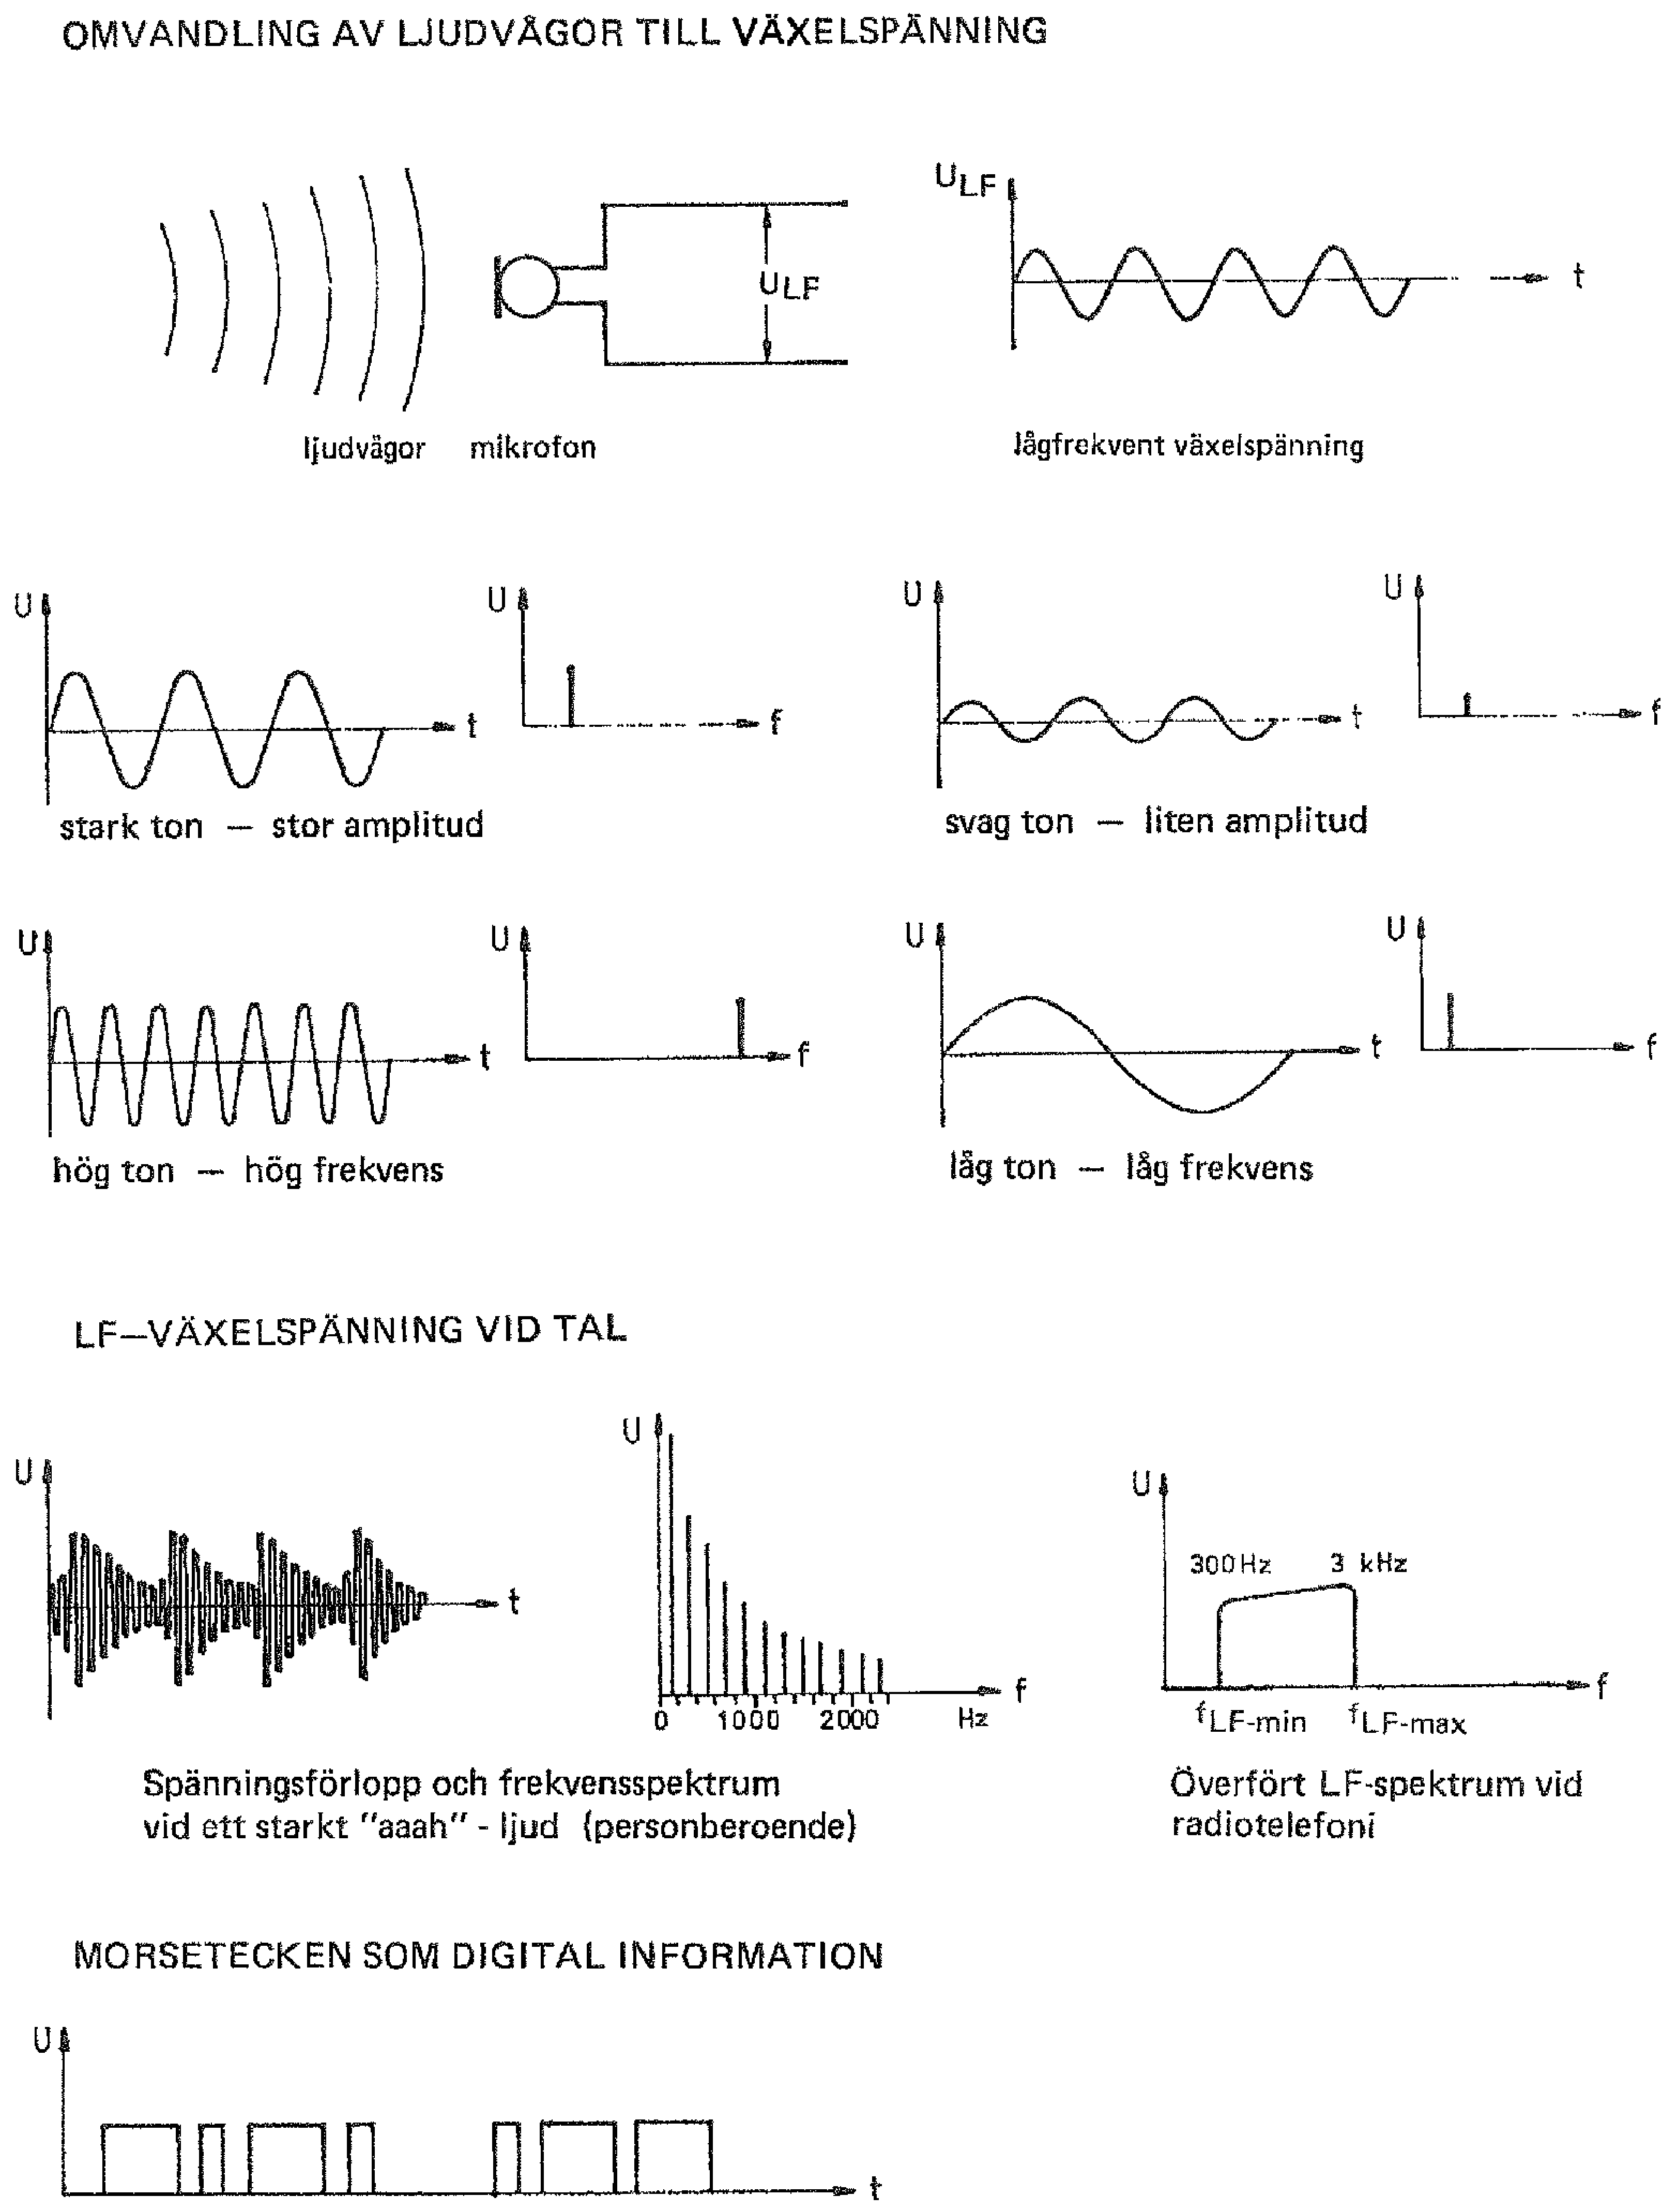
\includegraphics[width=\textwidth]{images/cropped_pdfs/bild_2_1-23.pdf}
\caption{Modulerande signaler}
\label{fig:BildII1-23}
\end{figure}

Bild \ref{fig:BildII1-23}.

Ett vanligt sätt att överföra information över radio är med telefoni, d.v.s.
tal.

Frekvensområdet 300--3000~Hz räcker för god förståelighet av tal. Dels är örat
känsligast inom det området och dels finns där den mesta energin i talet.

Mikrofonen tar upp de lufttrycksvariationer, som uppstår när man talar, och
omvandlar dem till elektriska svängningar. Svängningarna varierar mellan
positiva och negativa spänningsvärden.

\subsubsection{Försök}

\begin{enumerate}
\item Anslut en mikrofon till ett oscilloskop och studera spänningsförloppen
för olika slags ljud, toner, tal osv. som funktion av tiden. På bilden är
dessa svängningar mycket förenklade, t.ex. sinusformade.

\item Anslut en högtalare och ett oscilloskop till en LF-generator, vars
frekvens och amplitud kan ändras. Lyssna på ljud med låg och hög frekvens samt
på svaga och starka ljud. En baston har låg frekvens och en diskantton har hög
frekvens. En svag ton har liten amplitud och en stark ton har stor amplitud.
\end{enumerate}

\subsection{Sändningsslaget A3E (även kallat AM)}
\textbf{HAREC a.\ref{HAREC.a.1.8.2}, a.\ref{HAREC.a.1.8.6b}, a.\ref{HAREC.a.1.8.7b}\label{myHAREC.a.1.8.2}\label{myHAREC.a.1.8.6b}\label{myHAREC.a.1.8.7b}}
\index{amplitudmodulation}
\index{A3E}
\index{AM}

\begin{figure}
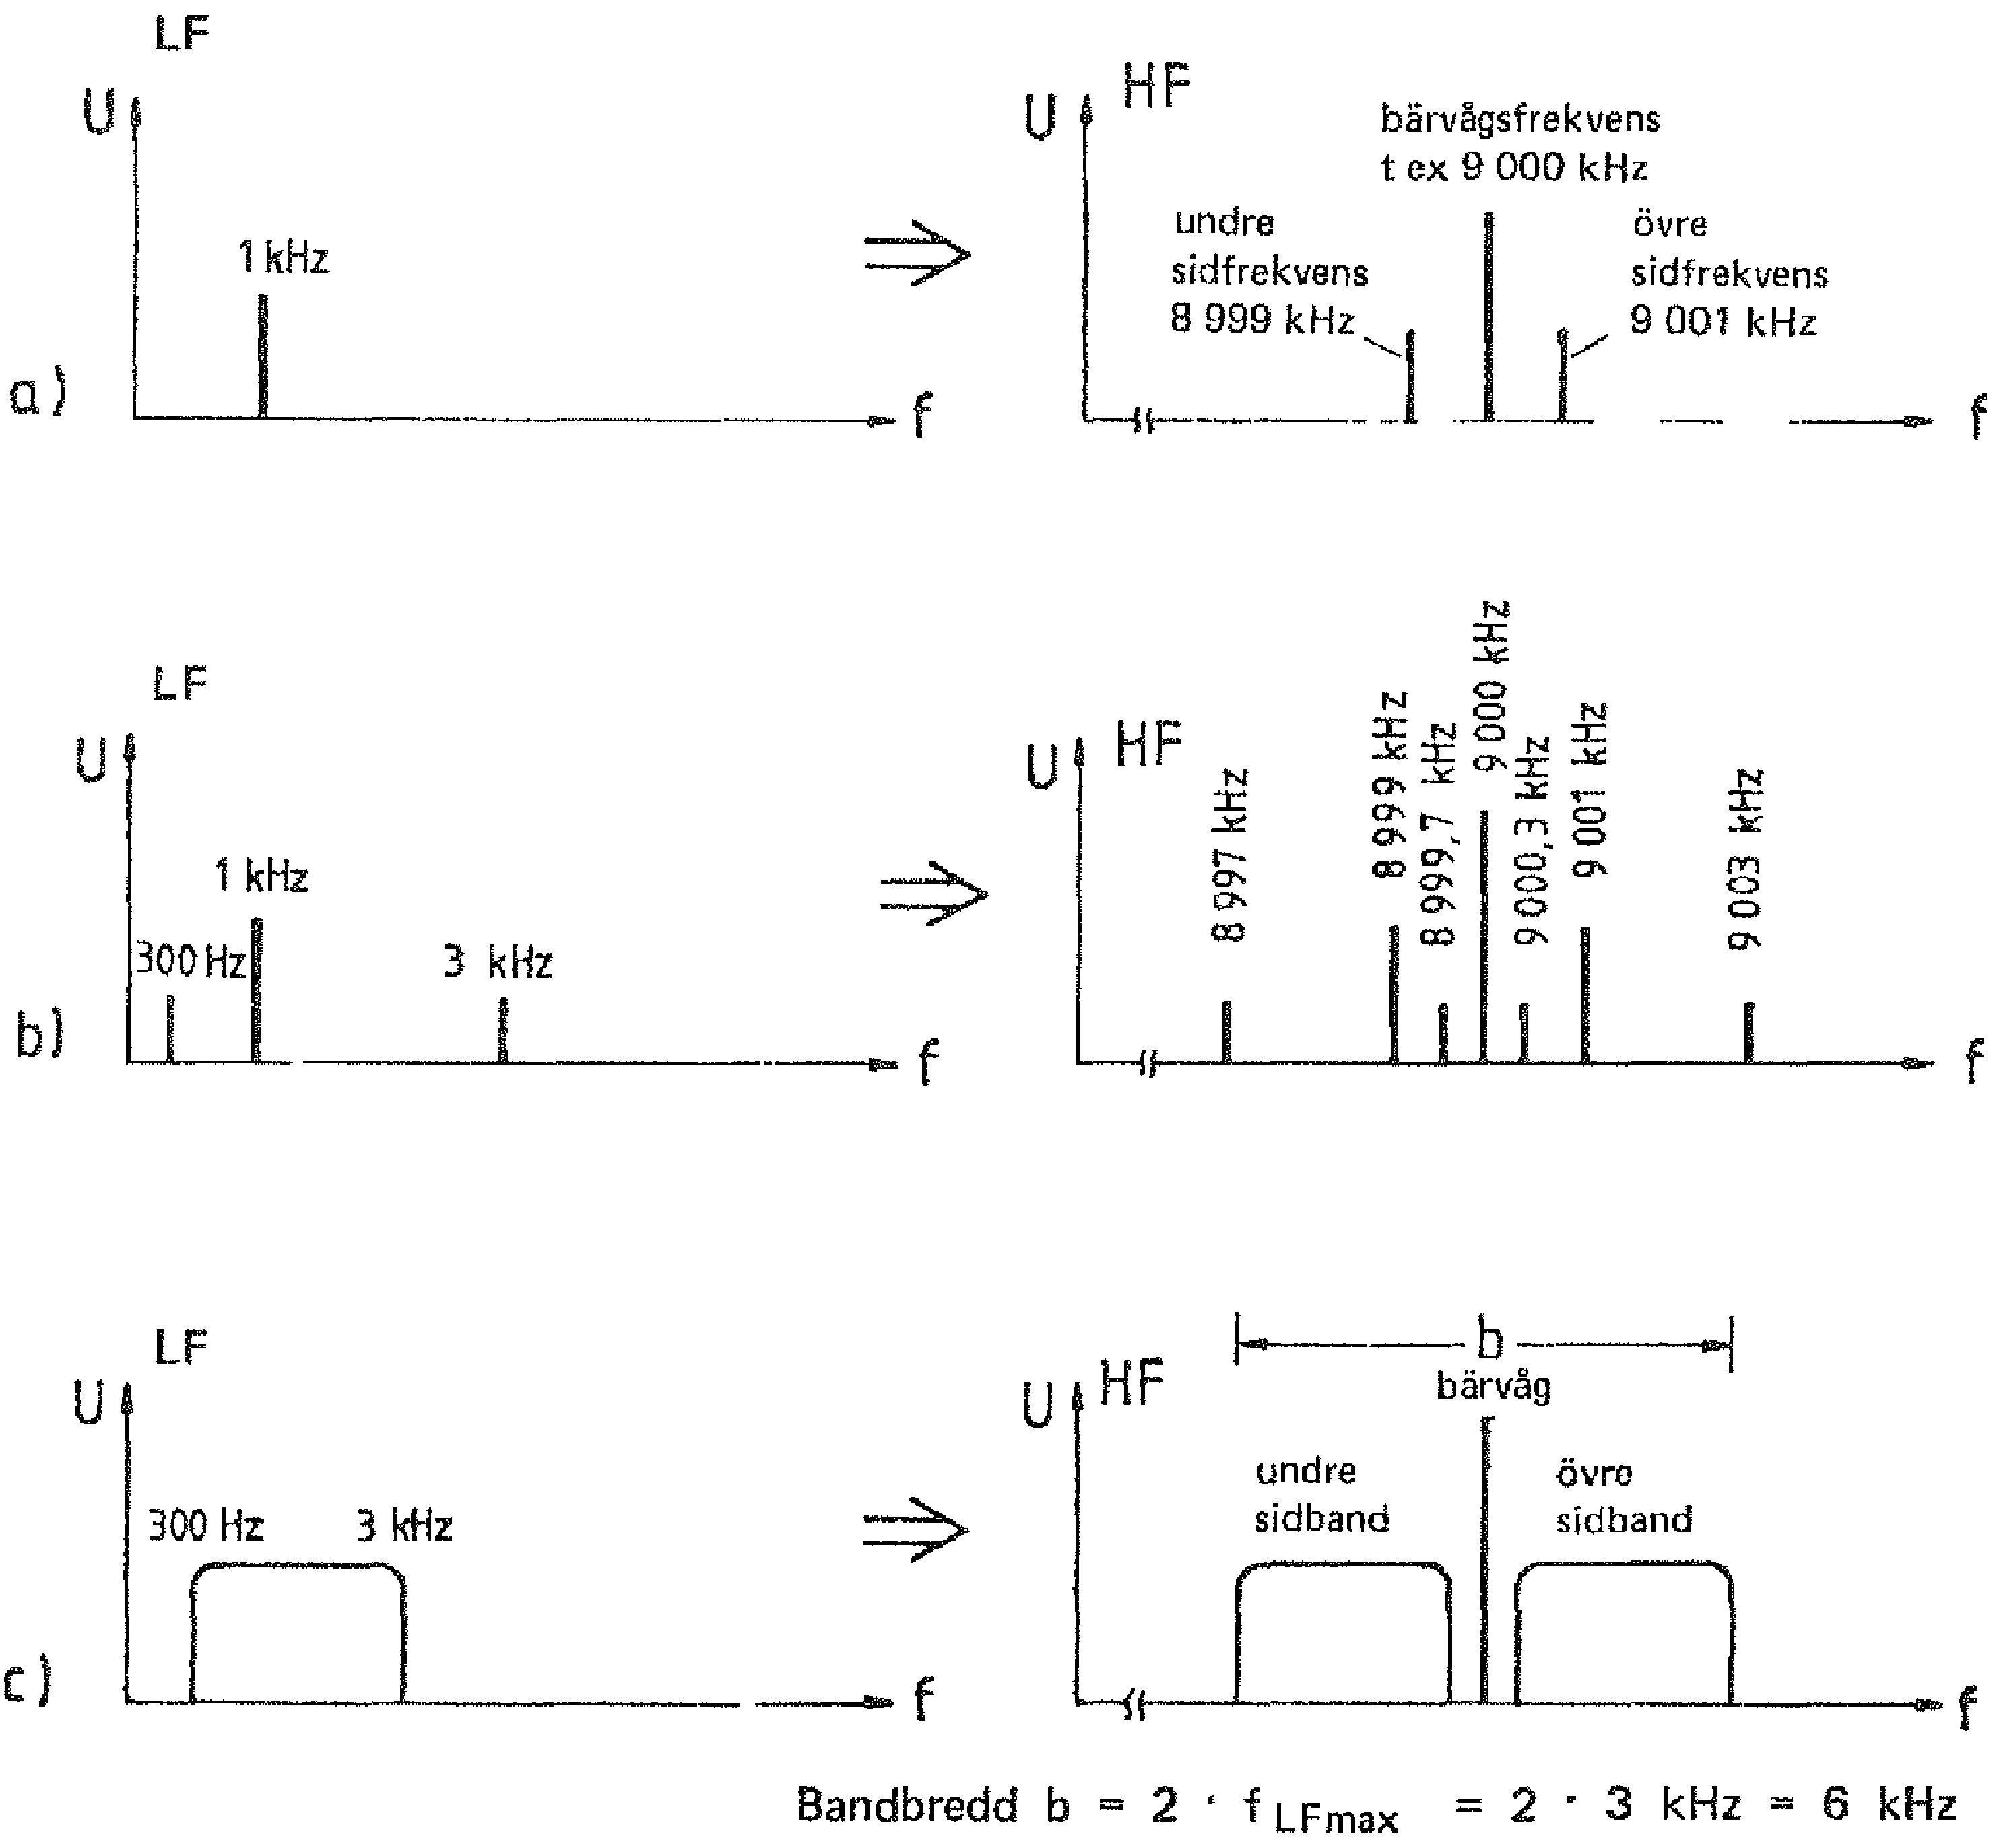
\includegraphics[width=\textwidth]{images/cropped_pdfs/bild_2_1-24.pdf}
\caption{Sidband vid A3E-modulation}
\label{fig:BildII1-24}
\end{figure}

Bild \ref{fig:BildII1-24}.

Bilden visar frekvensspektrum av en signal vid amplitudmodulation med

\begin{enumerate}[label=\alph*.,noitemsep]
\item en sinuston,
\item en blandning av tre sinustoner,
\item ett frekvensspektrum.
\end{enumerate}

\subsubsection{Försök}

Modulera en A3E-sändare med en 3~kHz signal. Med en mottagare utrustad med ett
smalt filter för telegrafi, kan man urskilja och påvisa bärvågen och de båda
sidbanden.

\subsubsection{A3E-modulation med en ton}

\begin{figure}
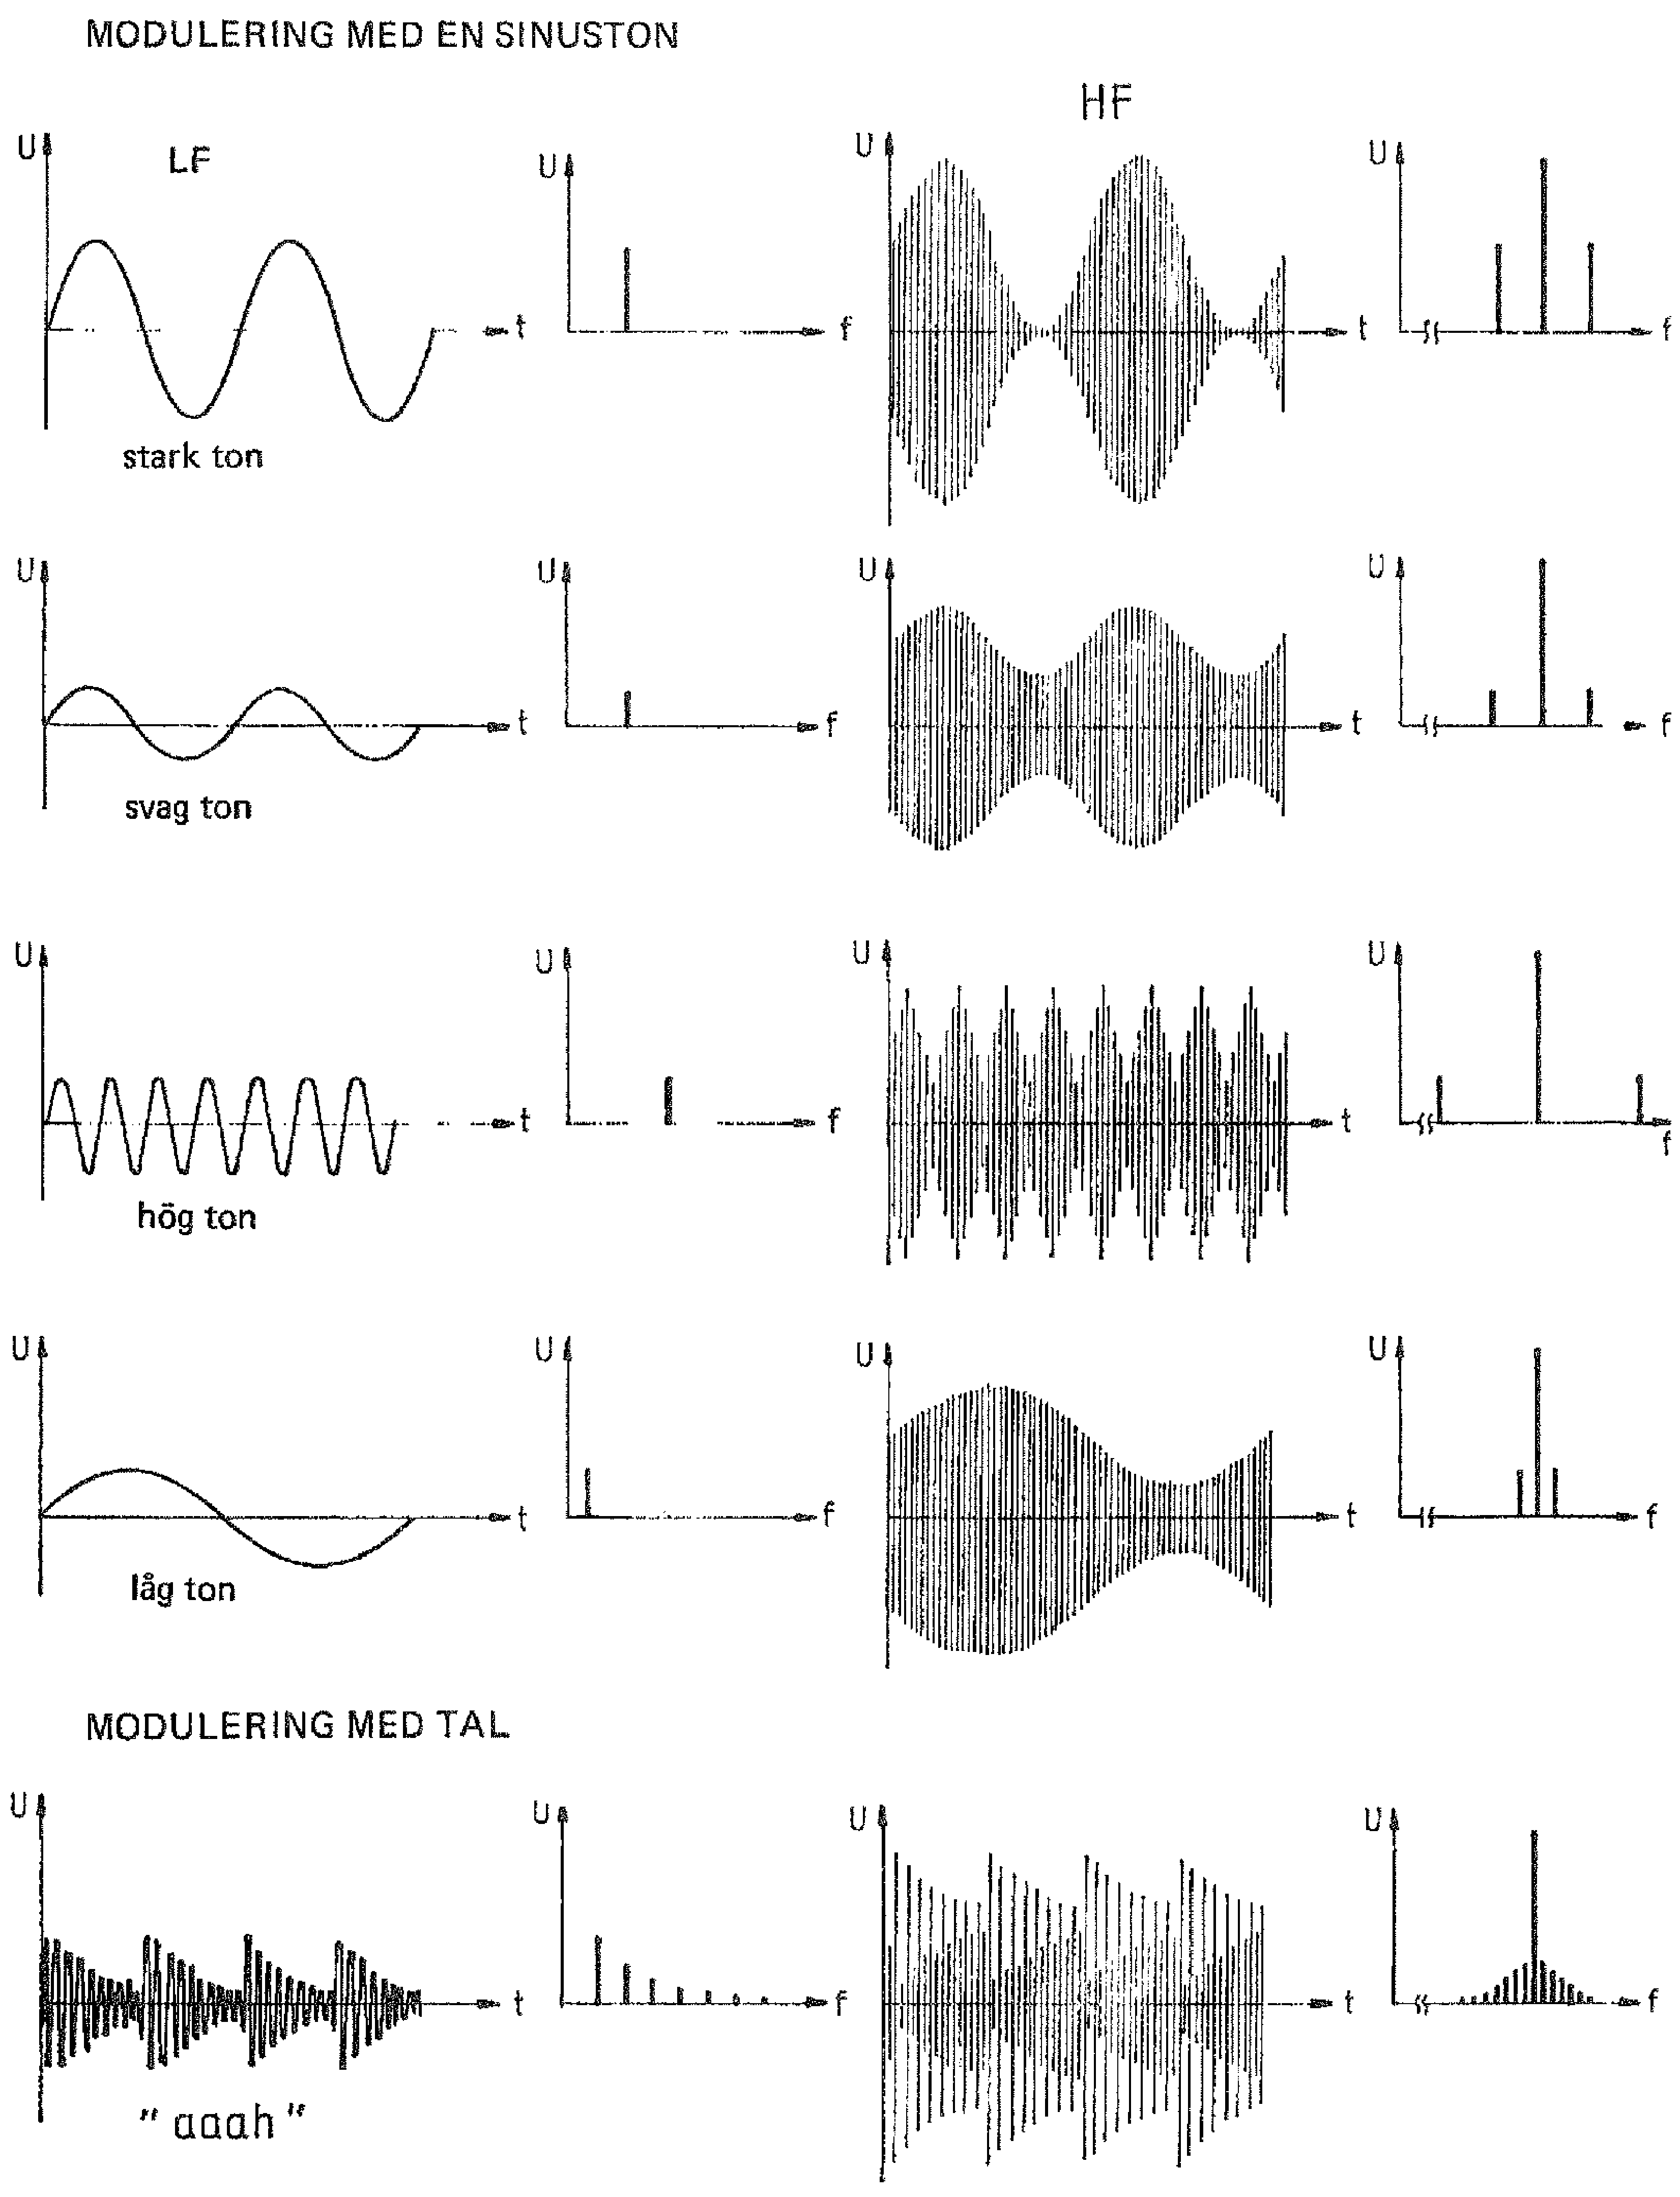
\includegraphics[width=\textwidth]{images/cropped_pdfs/bild_2_1-25.pdf}
\caption{A3E-modulation med toner med olika styrka och frekvens}
\label{fig:BildII1-25}
\end{figure}

Bild \ref{fig:BildII1-25}.

En omodulerad bärvåg har konstant amplitud. En amplitudmodulerad signal är i
grunden resultatet av svävning mellan frekvenser eller av icke linjär blandning
av frekvenser. När bärvåg och basband blandas, så är särskilt tre
blandningsprodukter av intresse.

Dessa är

\begin{enumerate}[label=-,noitemsep]
\item bärvågen,
\item det lägre sidbandet (förkortat LSB) och
\item det övre sidbandet (förkortat USB).
\end{enumerate}

AM-signalen består således inte bara av bärvågsfrekvensen \(f_{HF}\) utan även
av övre och nedre sidofrekvenser, vilka är summan och skillnaden av
bärvågsfrekvensen \(f_{HF}\) och den modulerande frekvensen \(f_{LF}\).
Alltså \(f_{HF} + f_{LF}\) (övre sidofrekvens) och skillnadsfrekvensen
\(f_{HF} - f_{LF}\) (undre sidofrekvens).

Eftersom tal inte bara omfattar en enda frekvens utan ett helt frekvensspektrum
(ca 0,3--3~kHz), så uppstår inte bara två sidofrekvenser utan två sidband, det
lägre sidbandet (LSB, Lower Side Band) och det övre (USB, Upper Side Band).

LF-signalens frekvens bestämmer sidofrekvensens avstånd från bärvågen.
Bandbredden på en amplitudmodulerad signal med full bärvåg och två sidband är
dubbelt så stor som den högsta modulerande LF-frekvensen:

\(b= 2 \cdot f_{LFmax}\)

Om de modulerande LF-frekvenserna är mellan 0,3 och 3~kHz, så blir sändningens
totala bandbredd 6~kHz.

LF-signalernas amplitud påverkar sidbandens och sidofrekvensernas amplitud. Vid
maximal modulation (100~\% modulationsgrad) varierar signalamplituden mellan
noll och dubbla värdet av det för en omodulerad bärvåg.

Som mest kan vardera sidbandet överföra en fjärdedel så mycket effekt som
bärvågen, d.v.s. en sjättedel av den totalt utsända effekten. Då avger sändaren
dubbelt så stor medeleffekt som utan modulation. Toppeffekten (PEP,
Peak Envelope Power) är till och med fyra gånger så stor.

Slutförstärkaren och kraftförsörjningen måste dimensioneras för toppeffekten vid
full modulation eller att modulationsgraden anpassas så att överbelastning inte
sker.

\subsubsection{Fördelar med A3E-modulation}

En A3E-sändare är enkel jämfört med en J3E-sändare, vilken har en mer
komplicerad signalbehandling.

\subsubsection{Nackdelar med A3E-modulation}

Eftersom samma information finns i båda sidbanden och ingen finns i bärvågen,
så sänds effekten i bärvågen och ett av sidbanden ut till ingen nytta. I
talpauser sänds endast bärvågseffekten och till ingen nytta. Även
frekvensutrymme slösas bort. Då en annan, alltför närliggande sändares bärvåg
blandas med den egna, så alstras interferenstoner i mottagarna.

\subsection{Sändningsslaget A1A (även kallat CW)}
\textbf{HAREC a.\ref{HAREC.a.1.8.1}, a.\ref{HAREC.a.1.8.6a}, a.\ref{HAREC.a.1.8.7a}\label{myHAREC.a.1.8.1}\label{myHAREC.a.1.8.6a}\label{myHAREC.a.1.8.7a}}
\index{A1A}
\index{CW}

\begin{figure}
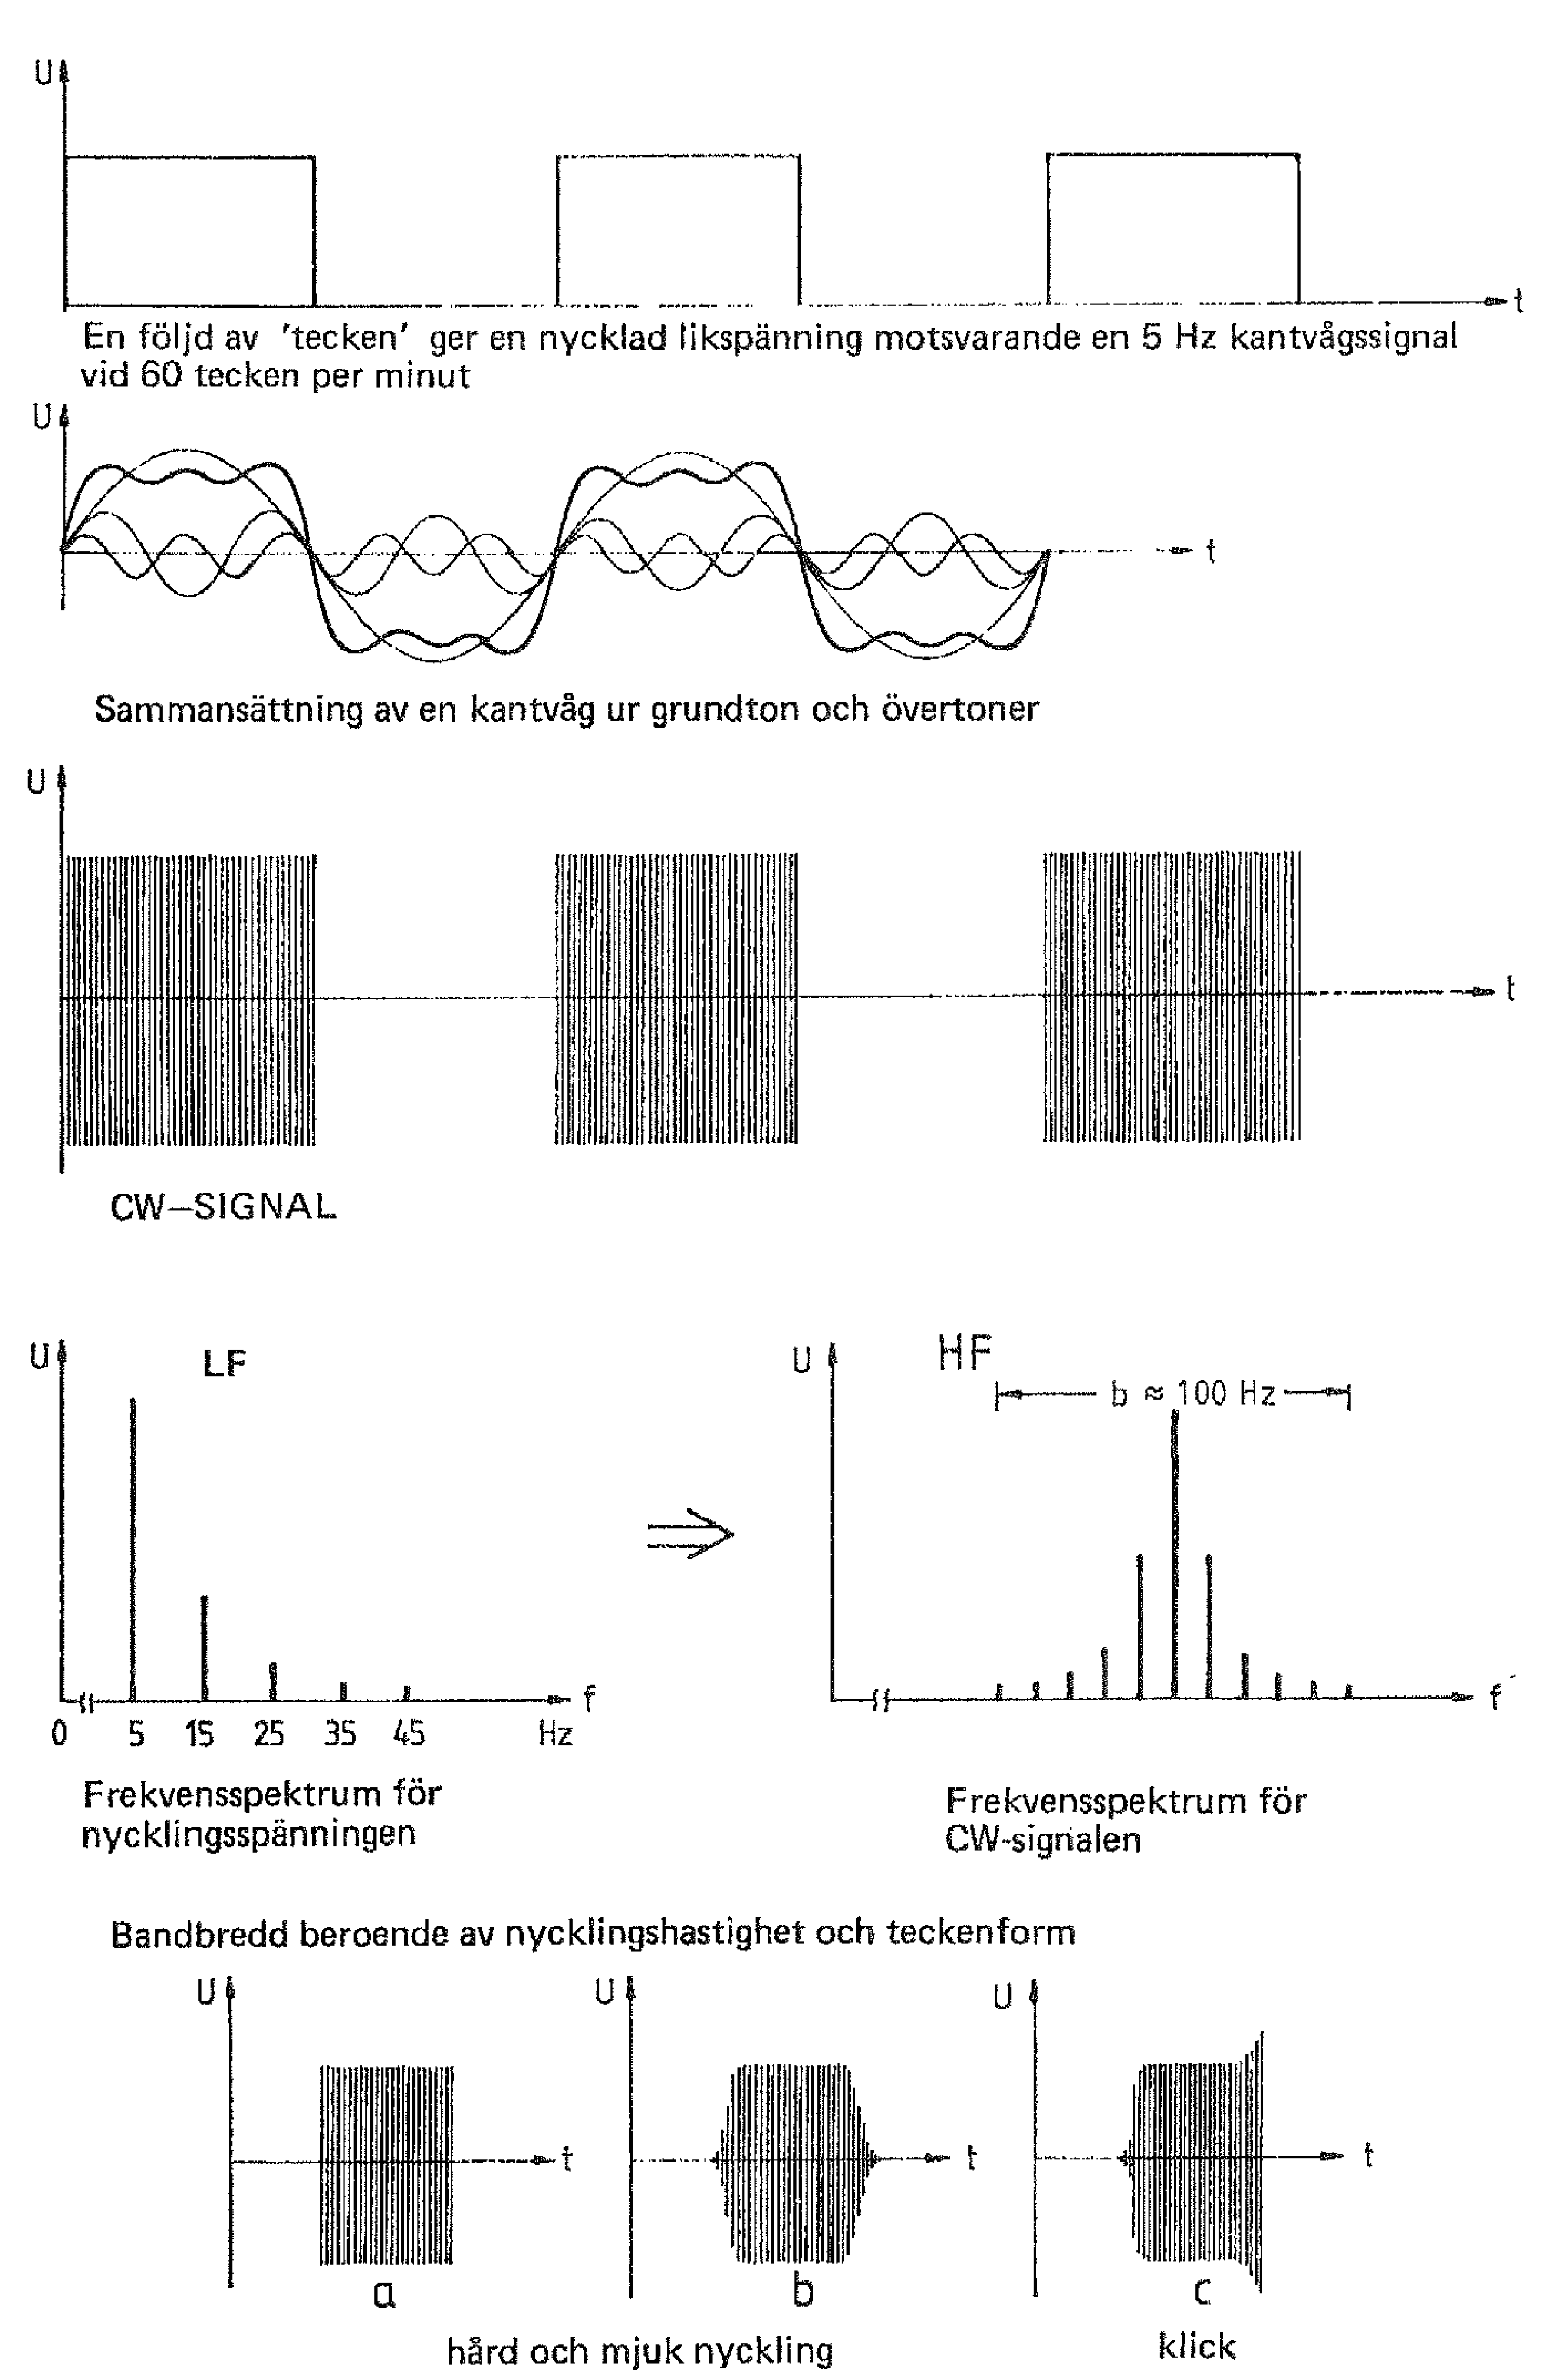
\includegraphics[width=\textwidth]{images/cropped_pdfs/bild_2_1-26.pdf}
\caption{Amplitudmodulation med morsetecken}
\label{fig:BildII1-26}
\end{figure}

Bild \ref{fig:BildII1-26}.

Man kan överföra meddelanden med morsetelegrafi på olika sätt. Det enklaste
sättet är att koppla in och ur sändarens bärvåg i takt med teckendelarna i
morsetecknen. Man kan kalla det för bärvågstelegrafi. Förfarandet kallas sedan
mycket länge även för CW (continous waves), vilket egentligen anger att
bärvågen svänger med konstant amplitud, om man bortser från att den nycklas.
Detta i motsats till de dämpade bärvågssvängningar som var fallet i sedan
mycket länge förbjudna s.k. gnistsändare.

Fastän en sändare ''moduleras utan ton'', har den en viss bandbredd. Det beror på
att den takt, som sändaren nycklas med, egentligen är en ton -- låt vara med låg
frekvens. Antag att sändaren nycklas med en serie korta morsetecken. Vid
telegraferingshastigheten 60 tecken/minut alstrar bärvågspulserna en kantvåg
med frekvensen 5~Hz. Som tidigare beskrivits, består en sådan kantvåg av summan
av sinussignaler med frekvenserna 5~Hz, 15~Hz, 25~Hz, 35~Hz o.s.v.

Det innebär att det uppstår sidofrekvenser över och under bärvågens frekvens och
med ett avstånd till bärvågen av 5~Hz, 15~Hz, 25~Hz, 35~Hz o.s.v.
Telegrafisändaren har alltså liksom vid A3E en bandbredd, som dels står i
förhållande till nycklingshastigheten och dels till ''kantigheten'' på tecknen,
vilket bestämmer övertonshalten i bärvågen. Vid s.k. mjuk nyckling kan den 9:e
övertonen antas vara den högsta som uppfattas av en motstation. Med en
nycklingsfrekvens av 5~Hz blir bandbredden inte större än
\(2 \cdot 10 \cdot 5 = 100\ Hz\).

En hård (kantig) och snabb teckengivning ökar bandbredden och kan resultera i
att s.k. nycklingsknäppar kan uppfattas långt vid sidan om sändningsfrekvensen.
Ju hårdare nycklingen är, desto längre bort från bärvågsfrekvensen hörs
nycklingsknäpparna. Detta stör andra stationer.

Kännetecken för sändningsslaget A1A, telegrafi genom nycklad bärvåg:

Mycket liten bandbredd, extremt gott utnyttjande av sändareffekten, stor
överföringssäkerhet, lång räckvidd, enkla sändare.

\subsection{Sändningsslaget J3E (även kallat SSB)}
\textbf{HAREC a.\ref{HAREC.a.1.8.3c}, a.\ref{HAREC.a.1.8.6c}, a.\ref{HAREC.a.1.8.7c}\label{myHAREC.a.1.8.3c}\label{myHAREC.a.1.8.6c}\label{myHAREC.a.1.8.7c}}
\index{single side band}
\index{J3E}
\index{SSB}

\subsubsection{Princip}

Som sagts är det onödigt sända ut två sidband, eftersom båda innehåller samma
information.

Signaler med endast ett sidband och undertryckt bärvåg kan alstras på flera
sätt. Numera är den s.k. filtermetoden i särklass vanligast och den enda som
behandlas här.

\begin{figure}
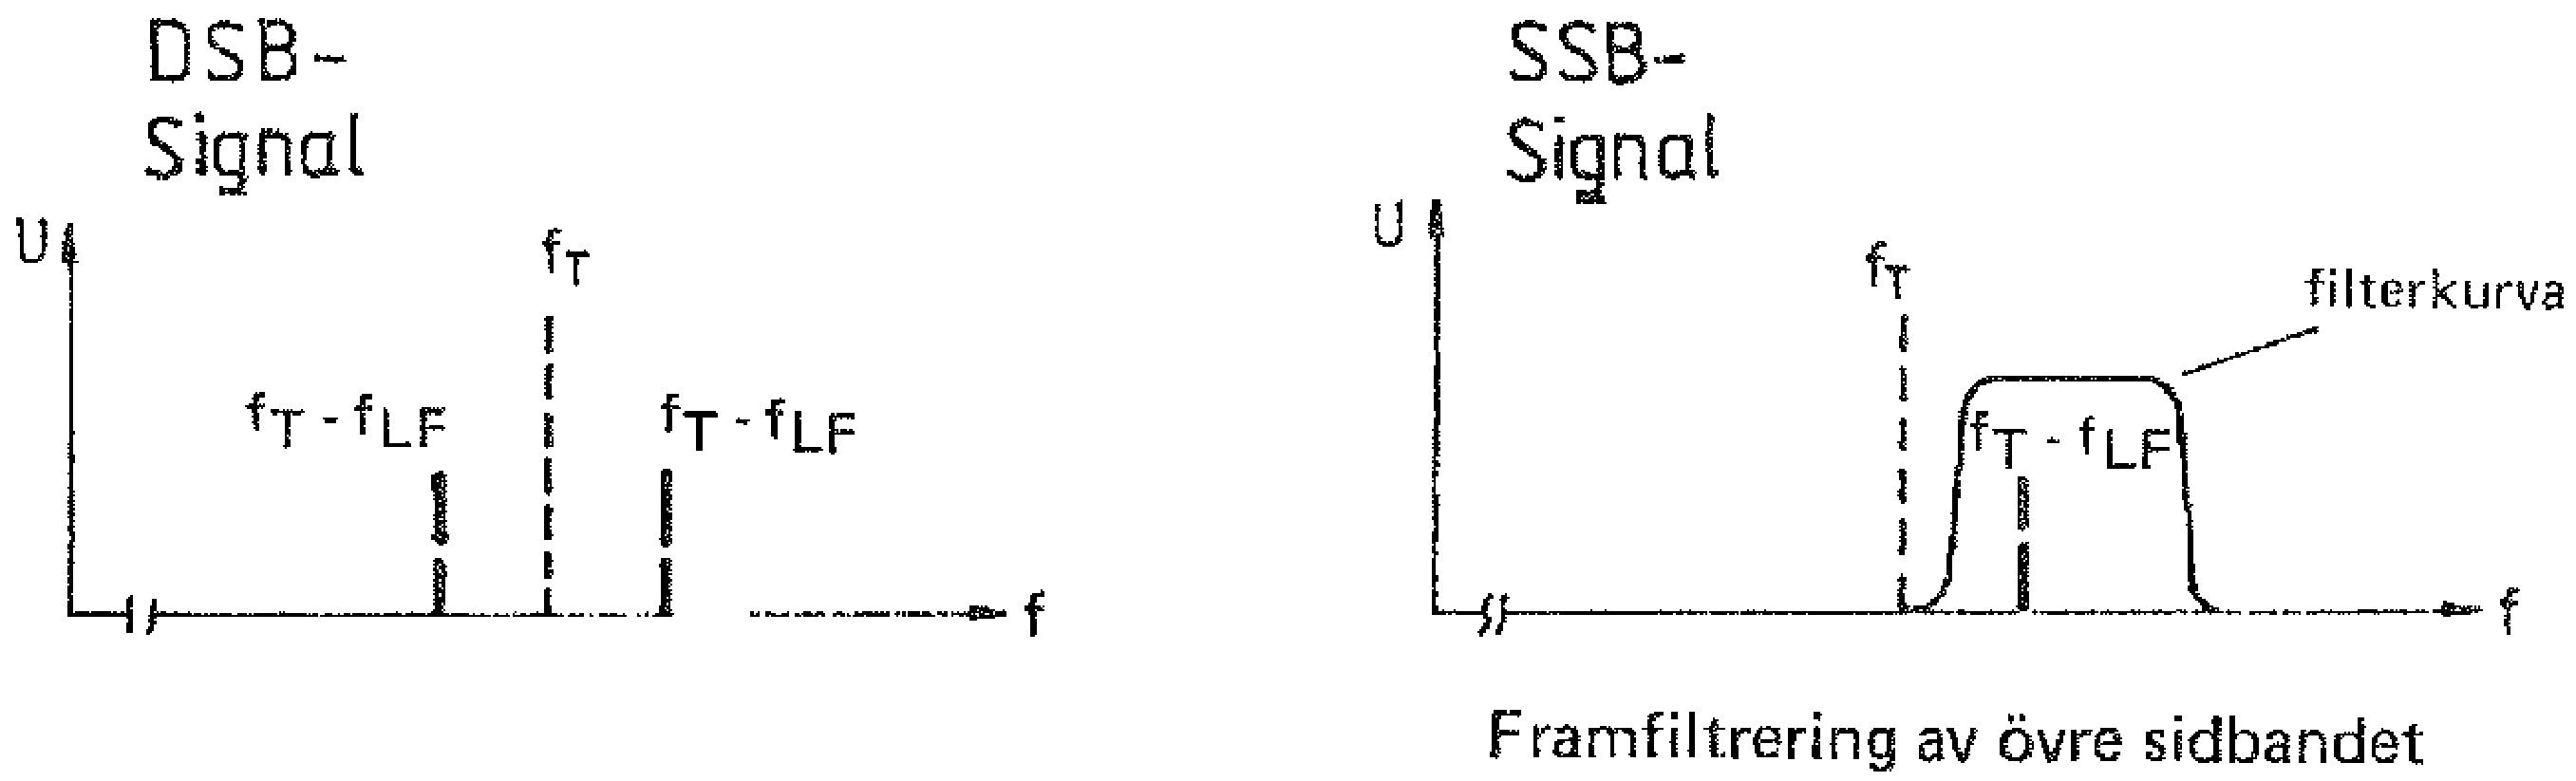
\includegraphics[width=\textwidth]{images/cropped_pdfs/bild_2_1-27.pdf}
\caption{Sidband vid DSB}
\label{fig:BildII1-27}
\end{figure}

Bild \ref{fig:BildII1-27}.

Med filtermetoden blandas HF- och LF-signalerna i en speciell blandare. Där
undertrycks båda dessa signaler medan blandningsprodukterna med deras summa-
och skillnadsfrekvenser blir kvar, d.v.s. det övre och nedre sidbandet.

Utsignalen från blandaren benämns DSB-signal (Double Side Band). Till skillnad
från i A3E-signalen saknas dock bärvågen i DSB-signalen. För att även
undertrycka det ena sidbandet före sändningen, så följs blandaren av ett
bandpassfilter med bandbredd och frekvensläge för avsett sidband.

Den signal som sänds ut innehåller därför endast ett sidband (Single Side Band).

\paragraph{Exempel}

\begin{figure}
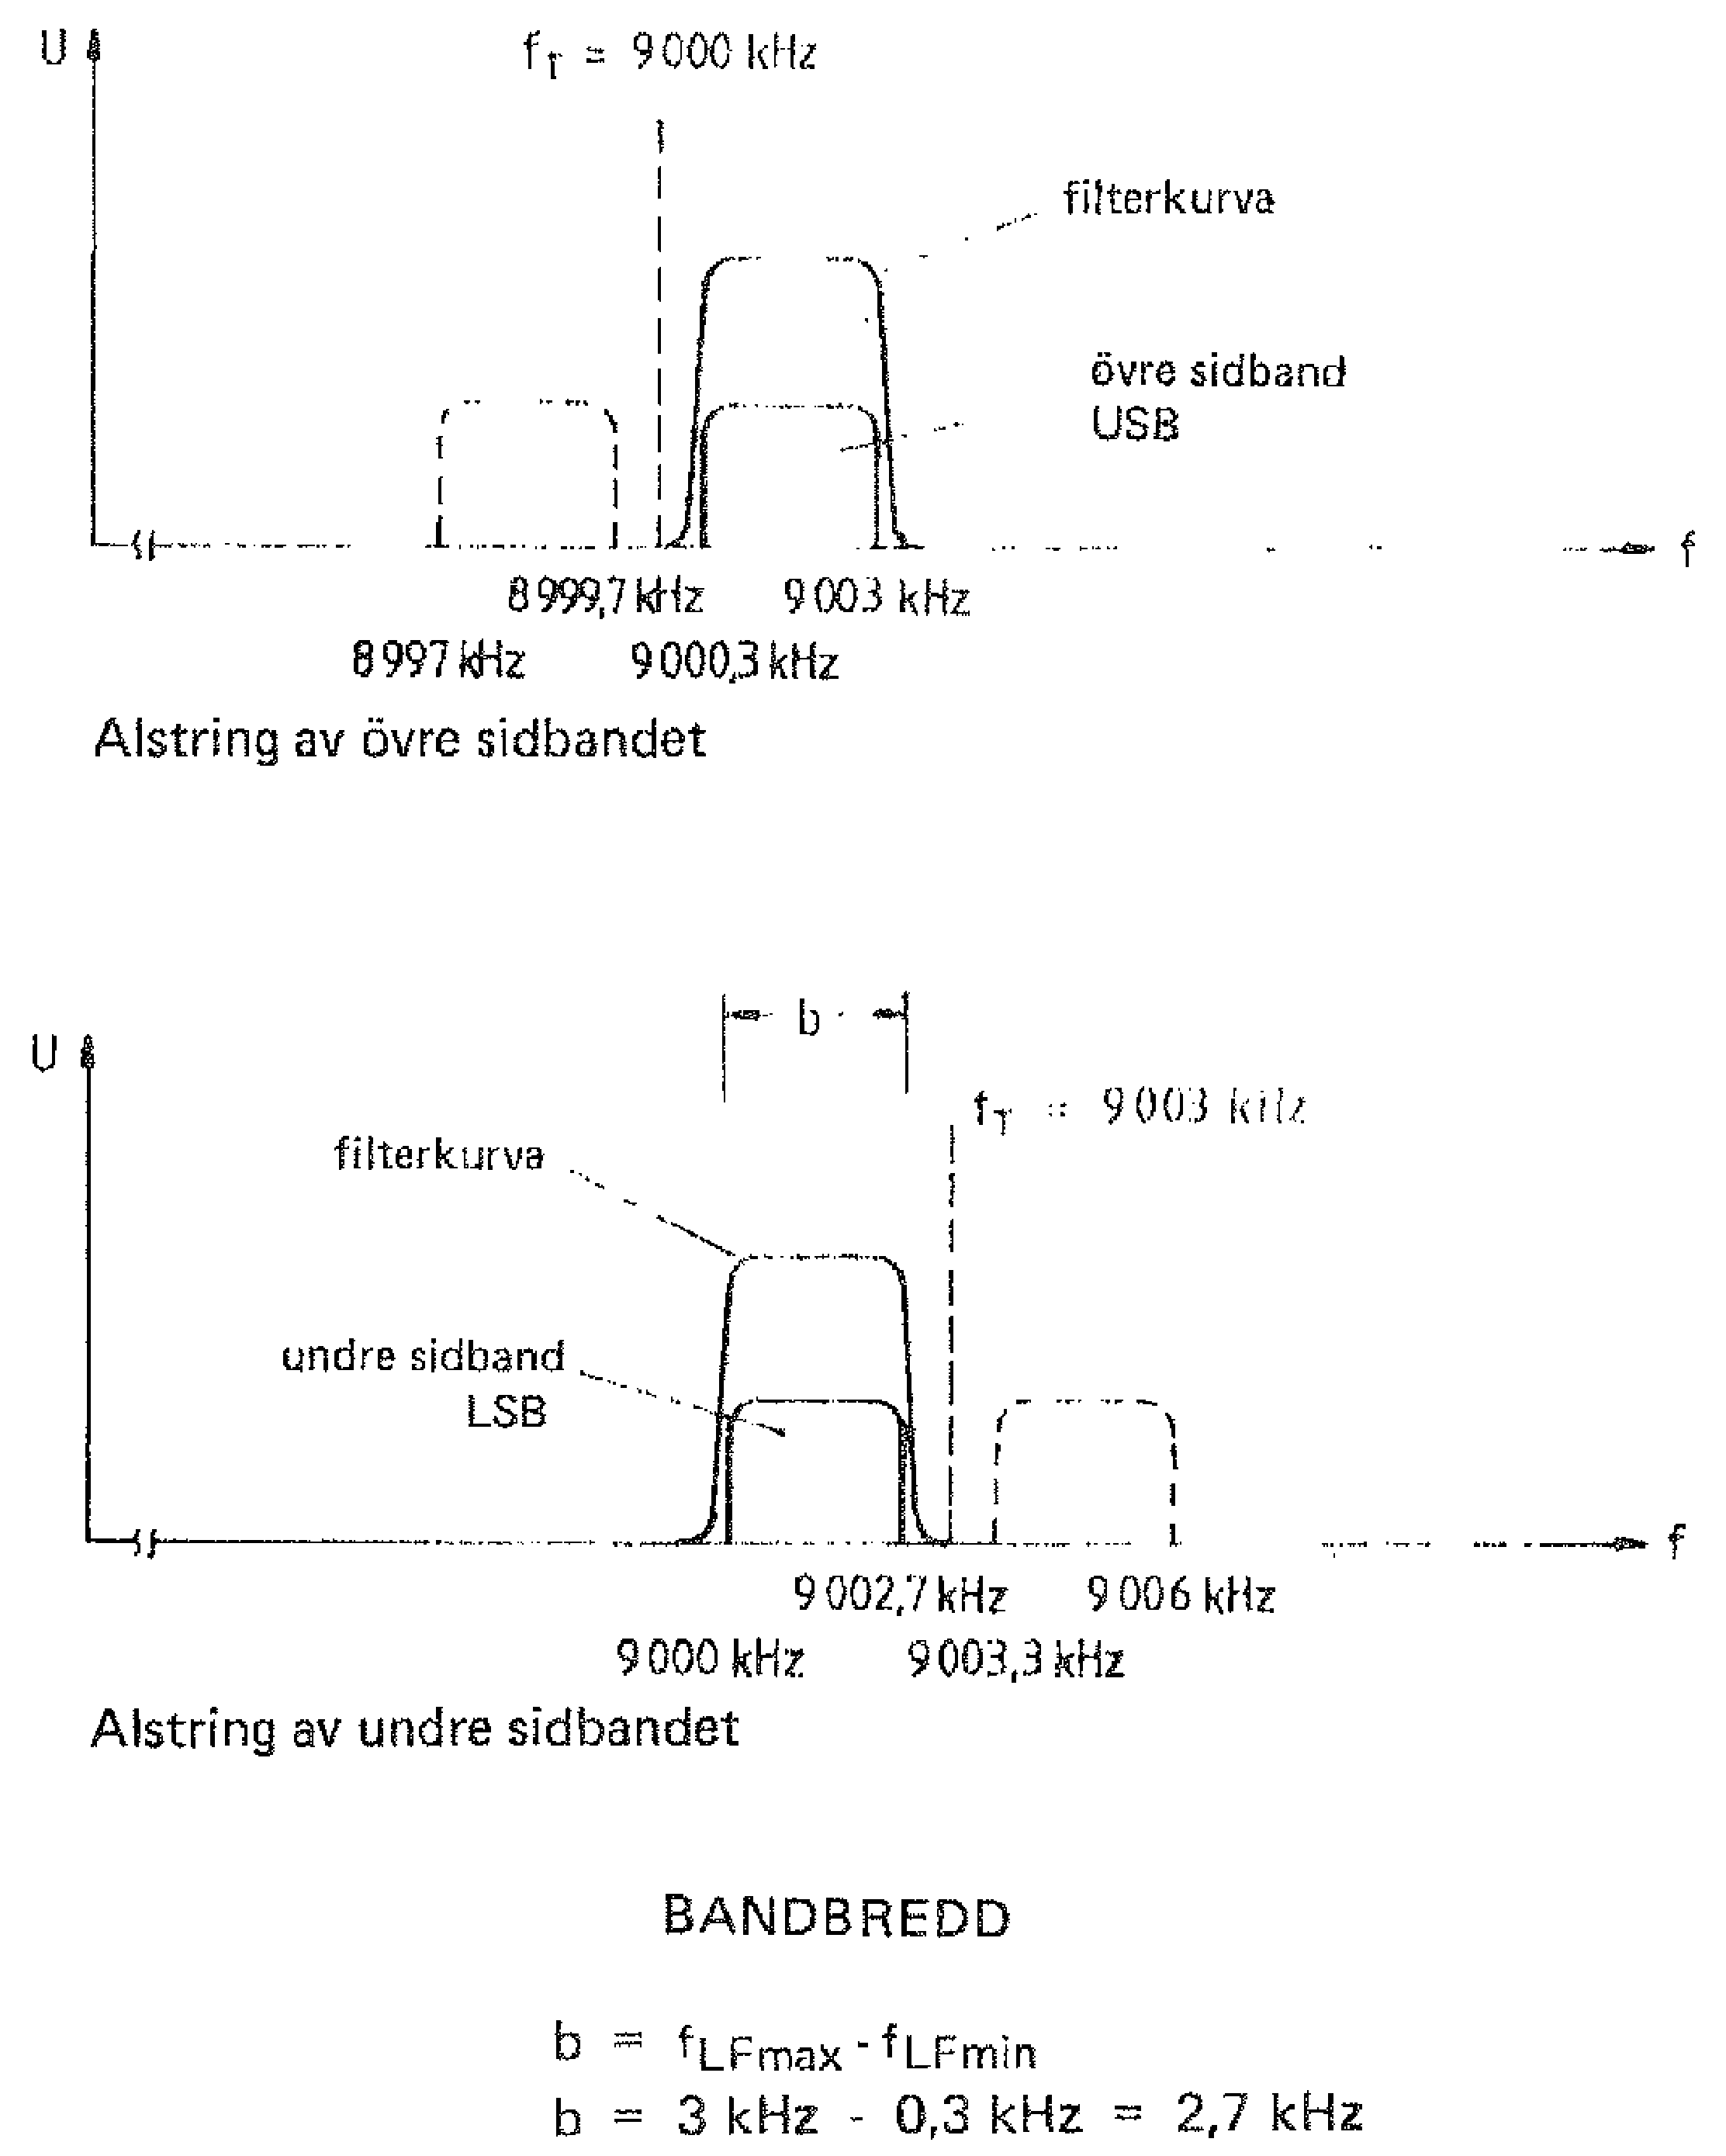
\includegraphics[width=\textwidth]{images/cropped_pdfs/bild_2_1-28.pdf}
\caption{Sidbandsval vid SSB}
\label{fig:BildII1-28}
\end{figure}

Bild \ref{fig:BildII1-28}.

Ett SSB-filter har ett passband av 9000,3--9003~kHz. Vid bärvågsfrekvensen 9000~kHz
sträcker sig det övre sidbandet från 9000,3--9003~kHz och släpps igenom. Däremot
blir bärvågsfrekvensen undertryckt.

Det undre sidbandet 8997--8999,7~kHz faller utanför filtrets passband och blir
också undertryckt.

Ska däremot det undre sidbandet kunna passera igenom samma filter, så måste
bärvågsfrekvensen höjas med 3~kHz, alltså till 9003~kHz. Då faller det undre
sidbandet, 9002,7--9000,0~kHz inom filtrets passband.

Det övre sidbandet 9003,3--9006,0~kHz faller nu utanför passbandet och blir
undertryckt.

\begin{figure}
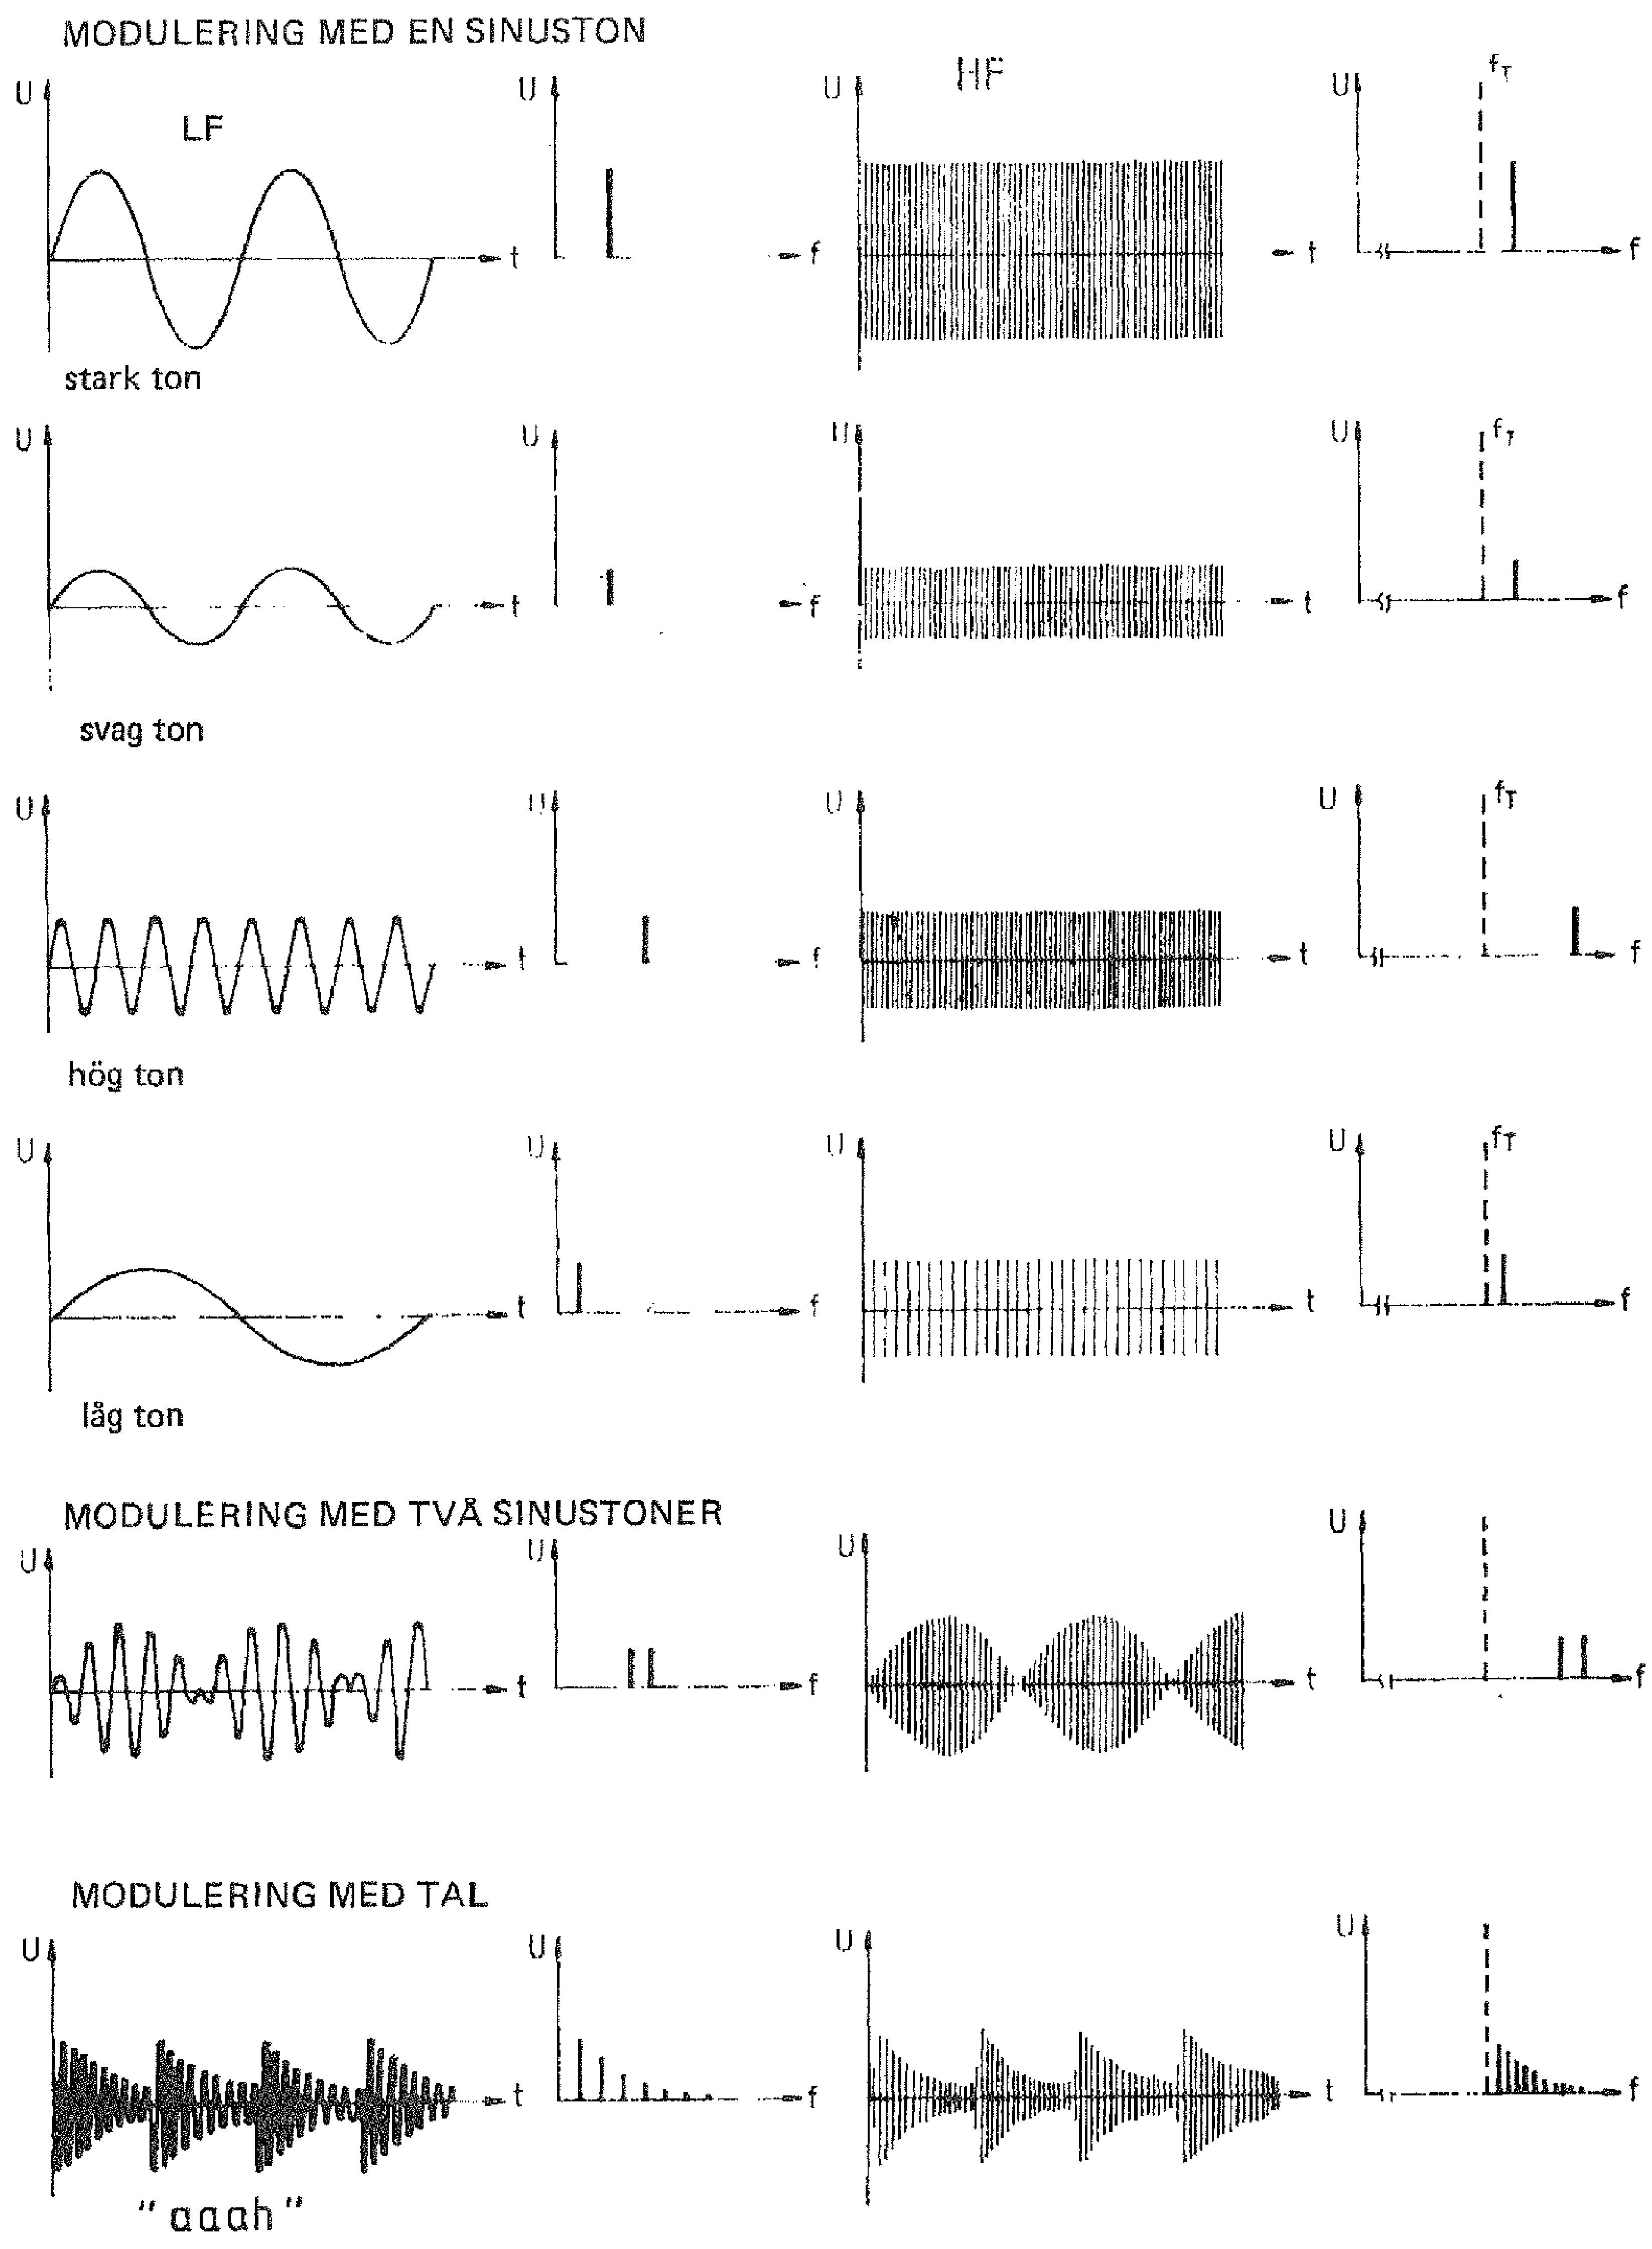
\includegraphics[width=\textwidth]{images/cropped_pdfs/bild_2_1-29.pdf}
\caption{Sidbandslägen vid SSB}
\label{fig:BildII1-29}
\end{figure}

Bild \ref{fig:BildII1-29}.

LF-signalens amplitud bestämmer amplituden på sidofrekvensen.

LF-signalens frekvens bestämmer sidofrekvensens avstånd från bärvågsfrekvensen
(bärvågen undertryckt).

Bandbredden på den utsända signalen är skillnaden mellan högsta och lägsta
modulerande frekvens i signalen:

t.ex. \(b = 3~kHz - 0,3~kHz = 2,7~kHz\)

\subsubsection{Fördelar med J3E-modulation}
Bra verkningsgrad vid J3E-modulation jämfört med vid A3E-modulation
(traditionell AM). Effekten i det utsända sidbandet motsvarar den i ett av
sidbanden vid A3E. Hela den utsända effekten finns alltså i ett enda sidband,
som överför hela informationen.

I sändningspauserna sänds ingen effekt ut. Bandbredden är mindre än hälften av
den vid A3E. Vid mottagning av en J3E-sändning (SSB) är det mindre besvär med
interferenstoner från J3E-sändningar på närliggande frekvenser, eftersom ingen
bärvåg och endast ett sidband sänds ut.

\subsubsection{Nackdelar med J3E-modulation}
J3E-modulation medför mera komplicerade apparater, både för mottagning och
sändning. En J3E-signal blir förvrängd och hörs i fel tonläge, om mottagaren
inte är inställd på exakt rätt frekvens.

\subsection{Vinkelmodulation}
\textbf{HAREC a.\ref{HAREC.a.1.8.3a}\label{myHAREC.a.1.8.3a}}
\index{vinkelmodulation}

Termen vinkelmodulation är samlingsnamnet för frekvensmodulation (FM) och
fasmodulation (PM). Ofta sägs utrustningar vara för frekvensmodulation, när de
antingen är för frekvens- eller fasmodulation. Det finns alltså skillnader och
likheter mellan dessa system, vilka emellertid inte är oberoende av varandra,
eftersom frekvensen i en signal inte kan varieras utan att fasen också
varieras, och vice versa.

Hur effektiv kommunikationen då är, beror mest på mottagningsmetoderna. I båda
fallen uppfattas ändringar i den mottagna signalens frekvens och fasläge.
Amplitudändringar uppfattas däremot inte. De flesta störningar -- särskilt
pulserande sådana som från tändningssystem -- kommer att därför att skiljas bort.

För att effektivt utnyttja fördelarna med vinkelmodulation, antingen det är
frekvens eller fasmodulation, behövs tillräckligt frekvensutrymme. Det innebär
att främst högre frekvensband kommer i fråga.

\subsection{Frekvensmodulation (även kallat FM)}
\textbf{HAREC
  a.\ref{HAREC.a.1.8.3b}\label{myHAREC.a.1.8.3b},
  a.\ref{HAREC.a.1.8.6d}\label{myHAREC.a.1.8.6d}
}
\index{frekvensmodulation}
\index{FM}

\begin{figure}
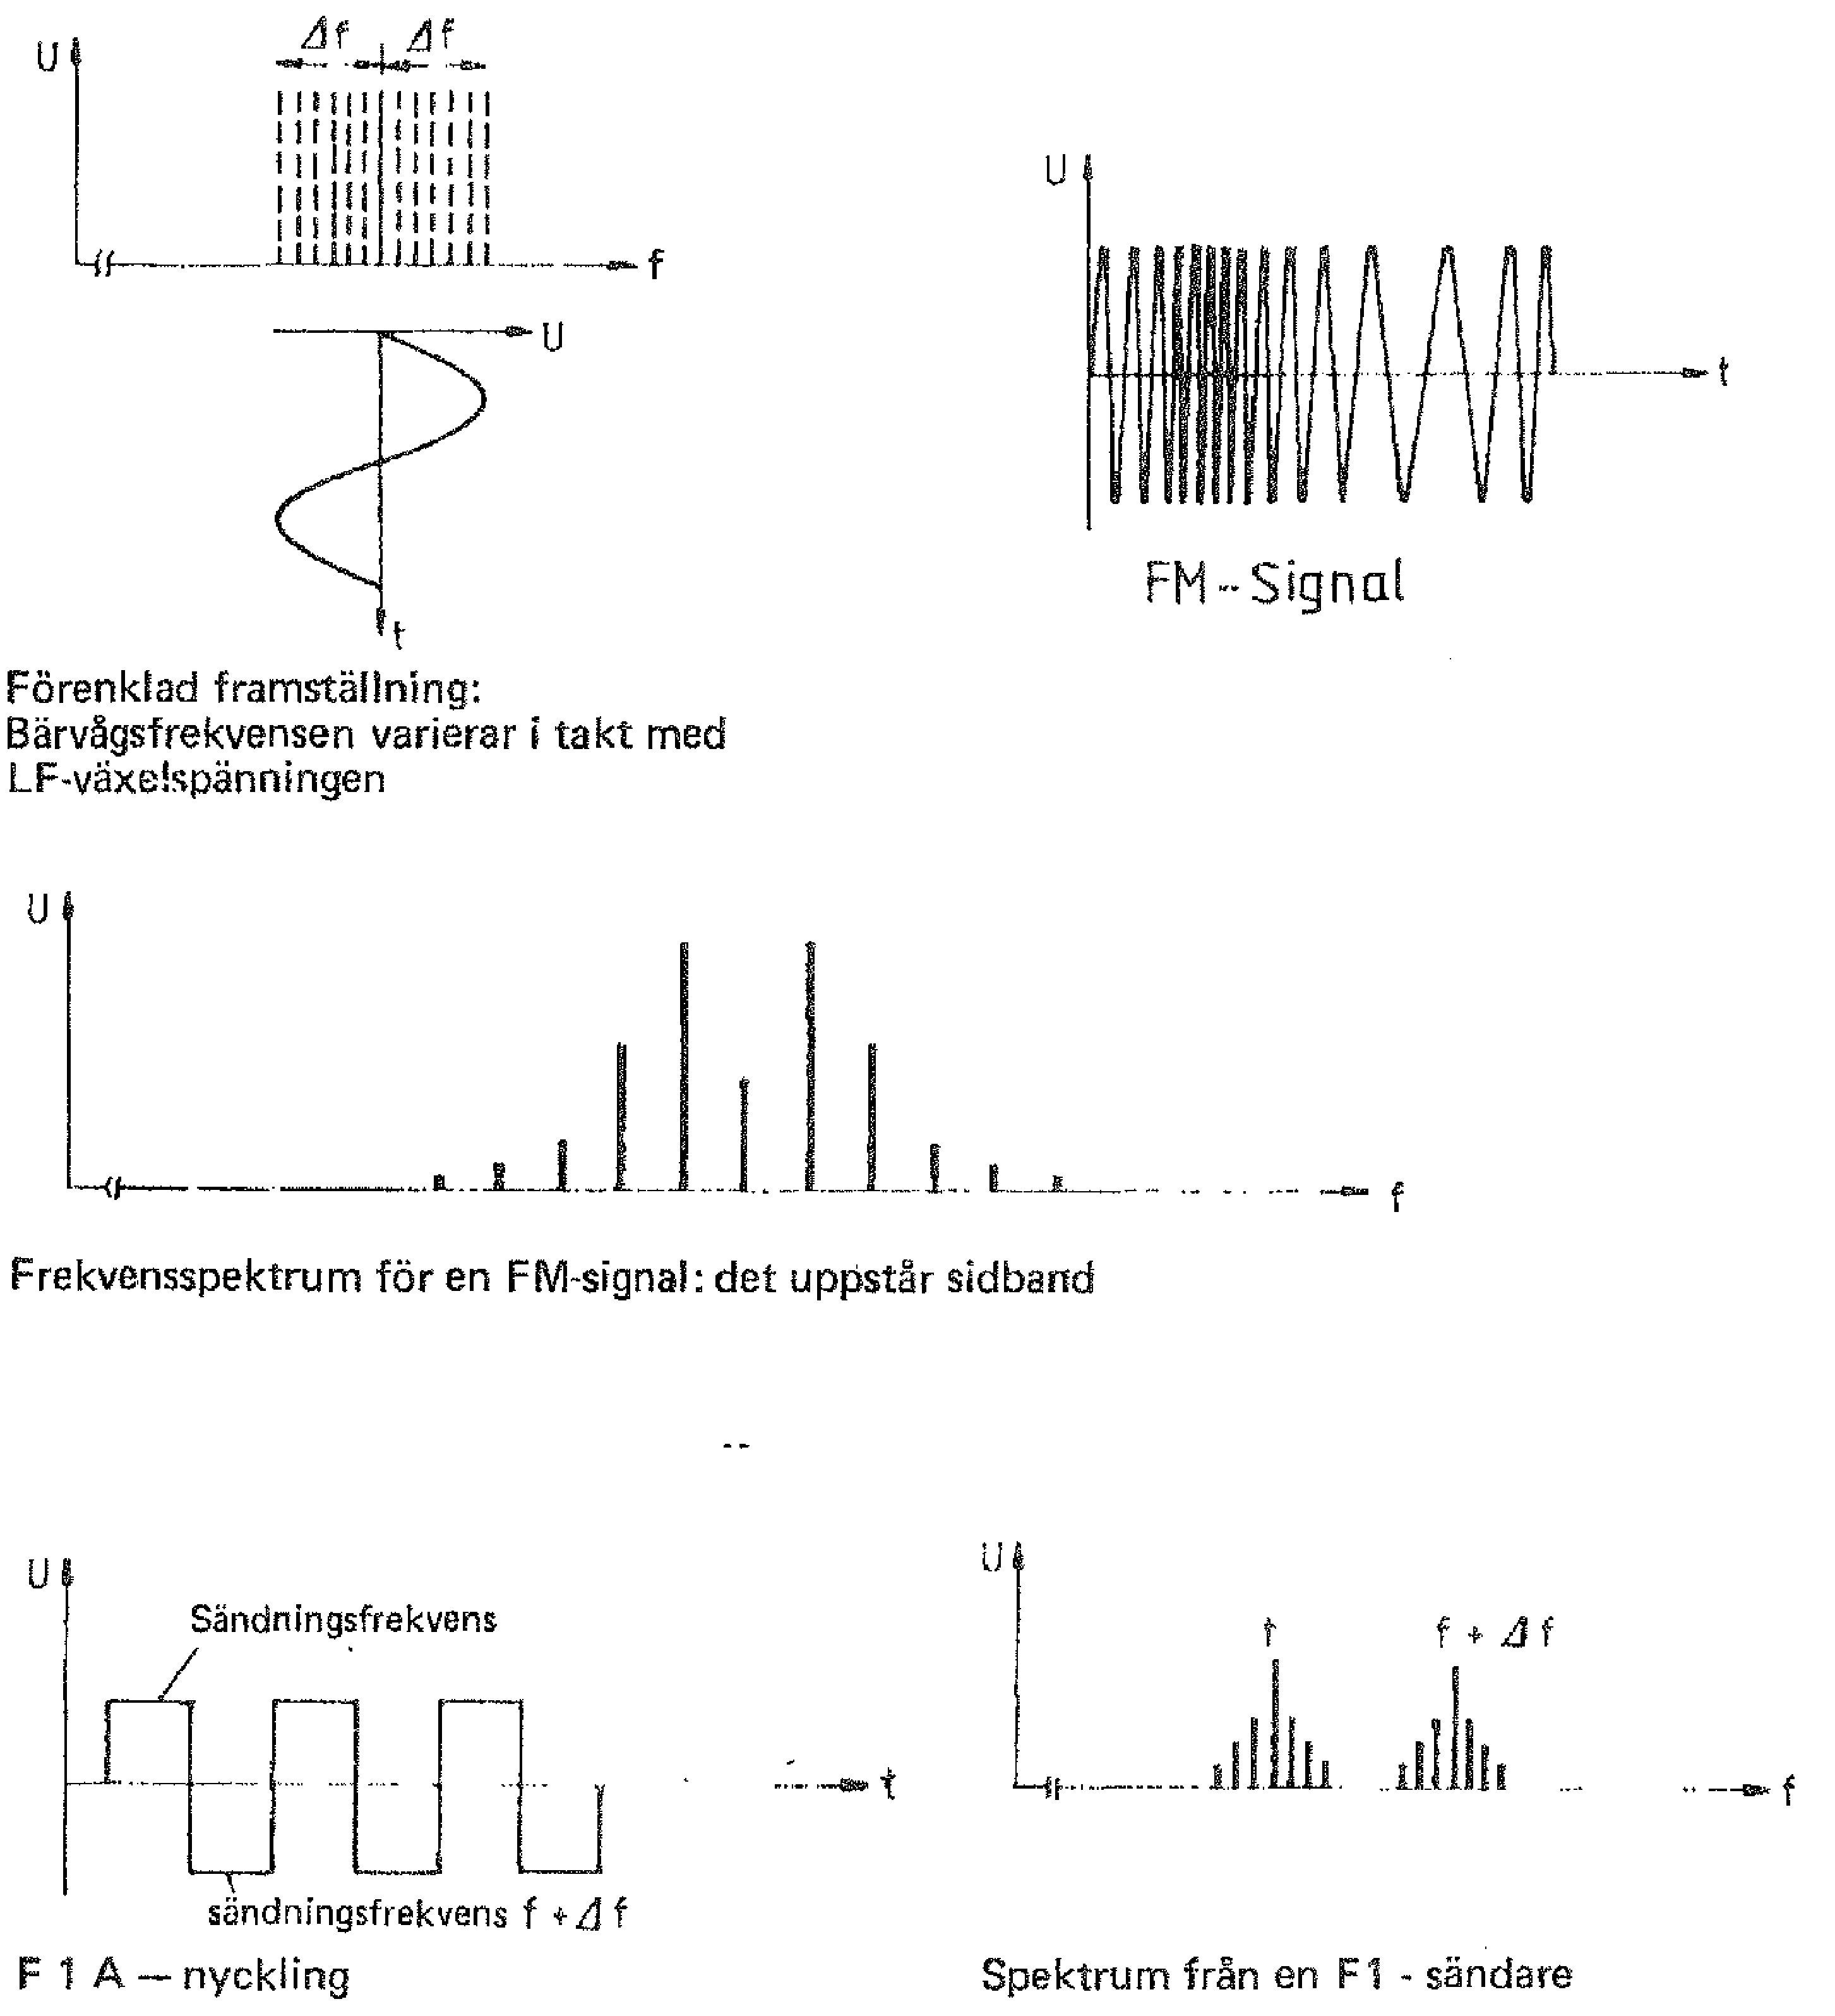
\includegraphics[width=\textwidth]{images/cropped_pdfs/bild_2_1-30.pdf}
\caption{Frekvensmodulation}
\label{fig:BildII1-30}
\end{figure}

Bild \ref{fig:BildII1-30} (överst och i mitten).

Vid frekvensmodulation varierar bärvågens frekvens i takt med den modulerande
signalens amplitud och polaritet. På bilden ökar bärvågens frekvens när den
modulerande signalen är positiv (första halvperioden) och minskar när den
modulerande signalen är negativ (andra halvperioden). Bilden visar att
perioderna i den modulerade bärvågen tar kortare tid (har högre frekvens), när
den modulerande signalen är positiv, och mertid (har lägre frekvens) när den
modulerande signalen är negativ. Bärvågen kommer alltså att pendla omkring ett
medelvärde, d.v.s. vara frekvensmodulerad.

Frekvensavvikelsen \(\Delta f\) (deviationen) från bärvågens vilofrekvens är
vid varje tillfälle proportionell till den modulerande signalens amplitud.
Sålunda är deviationen liten när den modulerande signalens amplitud är liten
och störst när amplituden når sitt toppvärde, antingen amplituden är positiv
eller negativ. Vid en modulationsfrekvens av 300~Hz varierar bärvågsfrekvensen
300 gånger per sekund, vid 3~kHz -- 3000 gånger per sekund.

Likspänningsnivåer kan överföras med FM, eftersom en motsvarande
frekvensavvikelse kan framställas.

Bilden visar också vad som oftast sägs, att bärvågsamplituden inte ändras av
modulationen. Detta är emellertid bara delvis sant, eftersom såväl
bärvågsamplitud som sidbandsamplitud varierar med modulationsindex, vilket
förklaras nedan.

\subsubsection{Sidbanden vid vinkelmodulation}

Vid AM produceras endast ett sidbandspar med samma innehåll, ett över och ett
under bärvågsfrekvensen. Vid vinkelmodulation, både vid FM och PM, produceras
däremot flera sidbandspar över och under bärvågsfrekvensen. Dessa sidband
uppträder på multiplerna av varje modulerande frekvens. Vid basband med samma
frekvensomfång har därför en vinkelmodulerad signal större bandbredd än en
AM-signal.

Vid vinkelmodulation beror antalet sidband på sambandet mellan den modulerande
frekvensen, frekvensdeviationen och modulationsindex.

\subsubsection{Bandbredden vid vinkelmodulation}

Bild \ref{fig:BildII1-30} (nederst).

Vi gör tankeexperimentet att en FM-sändare moduleras med en fyrkantsvåg.
Frekvensen kommer då att hoppa växelvis mellan frekvenserna \(f\) och
\(f + \Delta f\). Sättet kallas FSK (frekvensskiftnyckling) och används t.ex.
vid sändning av radiofjärrskrift (RTTY, AMTOR, Paketradio etc.).

Vi föreställer oss två sändare, som sänder varannan gång, varav den ena sänder
frekvensen \(f\) och den andra sänder \(f + \Delta f\). Båda sändarnas
HF-signaler kommer då att bilda ett frekvensspektrum, som förutom \(f\) och
\(f + \Delta f\) även innehåller sidofrekvenser.

Bredden på detta spektrum beror bl.a. på nycklingsfrekvensen. Eftersom en
fyrkantsvåg innehåller summan av dess grundfrekvens och övertoner, kommer alla
dessa toner att modulera vardera sändaren. De högsta modulerande
LF-frekvenserna alstrar sidofrekvenserna längst ut från vilofrekvensen.
LF-signalens frekvensspektrum påverkar alltså HF-signalens bandbredd.

Spektrum nederst i bilden är en förenklad framställning av
frekvensskiftnyckling.

Vid modulation med en sinussignal istället för med en fyrkantssignal, uppstår ett
frekvensspektrum som på överst i bilden.

\paragraph{Frekvensdeviation och modulationsindex}
\textbf{HAREC a.\ref{HAREC.a.1.8.4}\label{myHAREC.a.1.8.4}}
\index{frekvensdeviation}
\index{modulationsindex (m)}
\index{symbol!\(m\) modulationsindex}

\begin{figure}
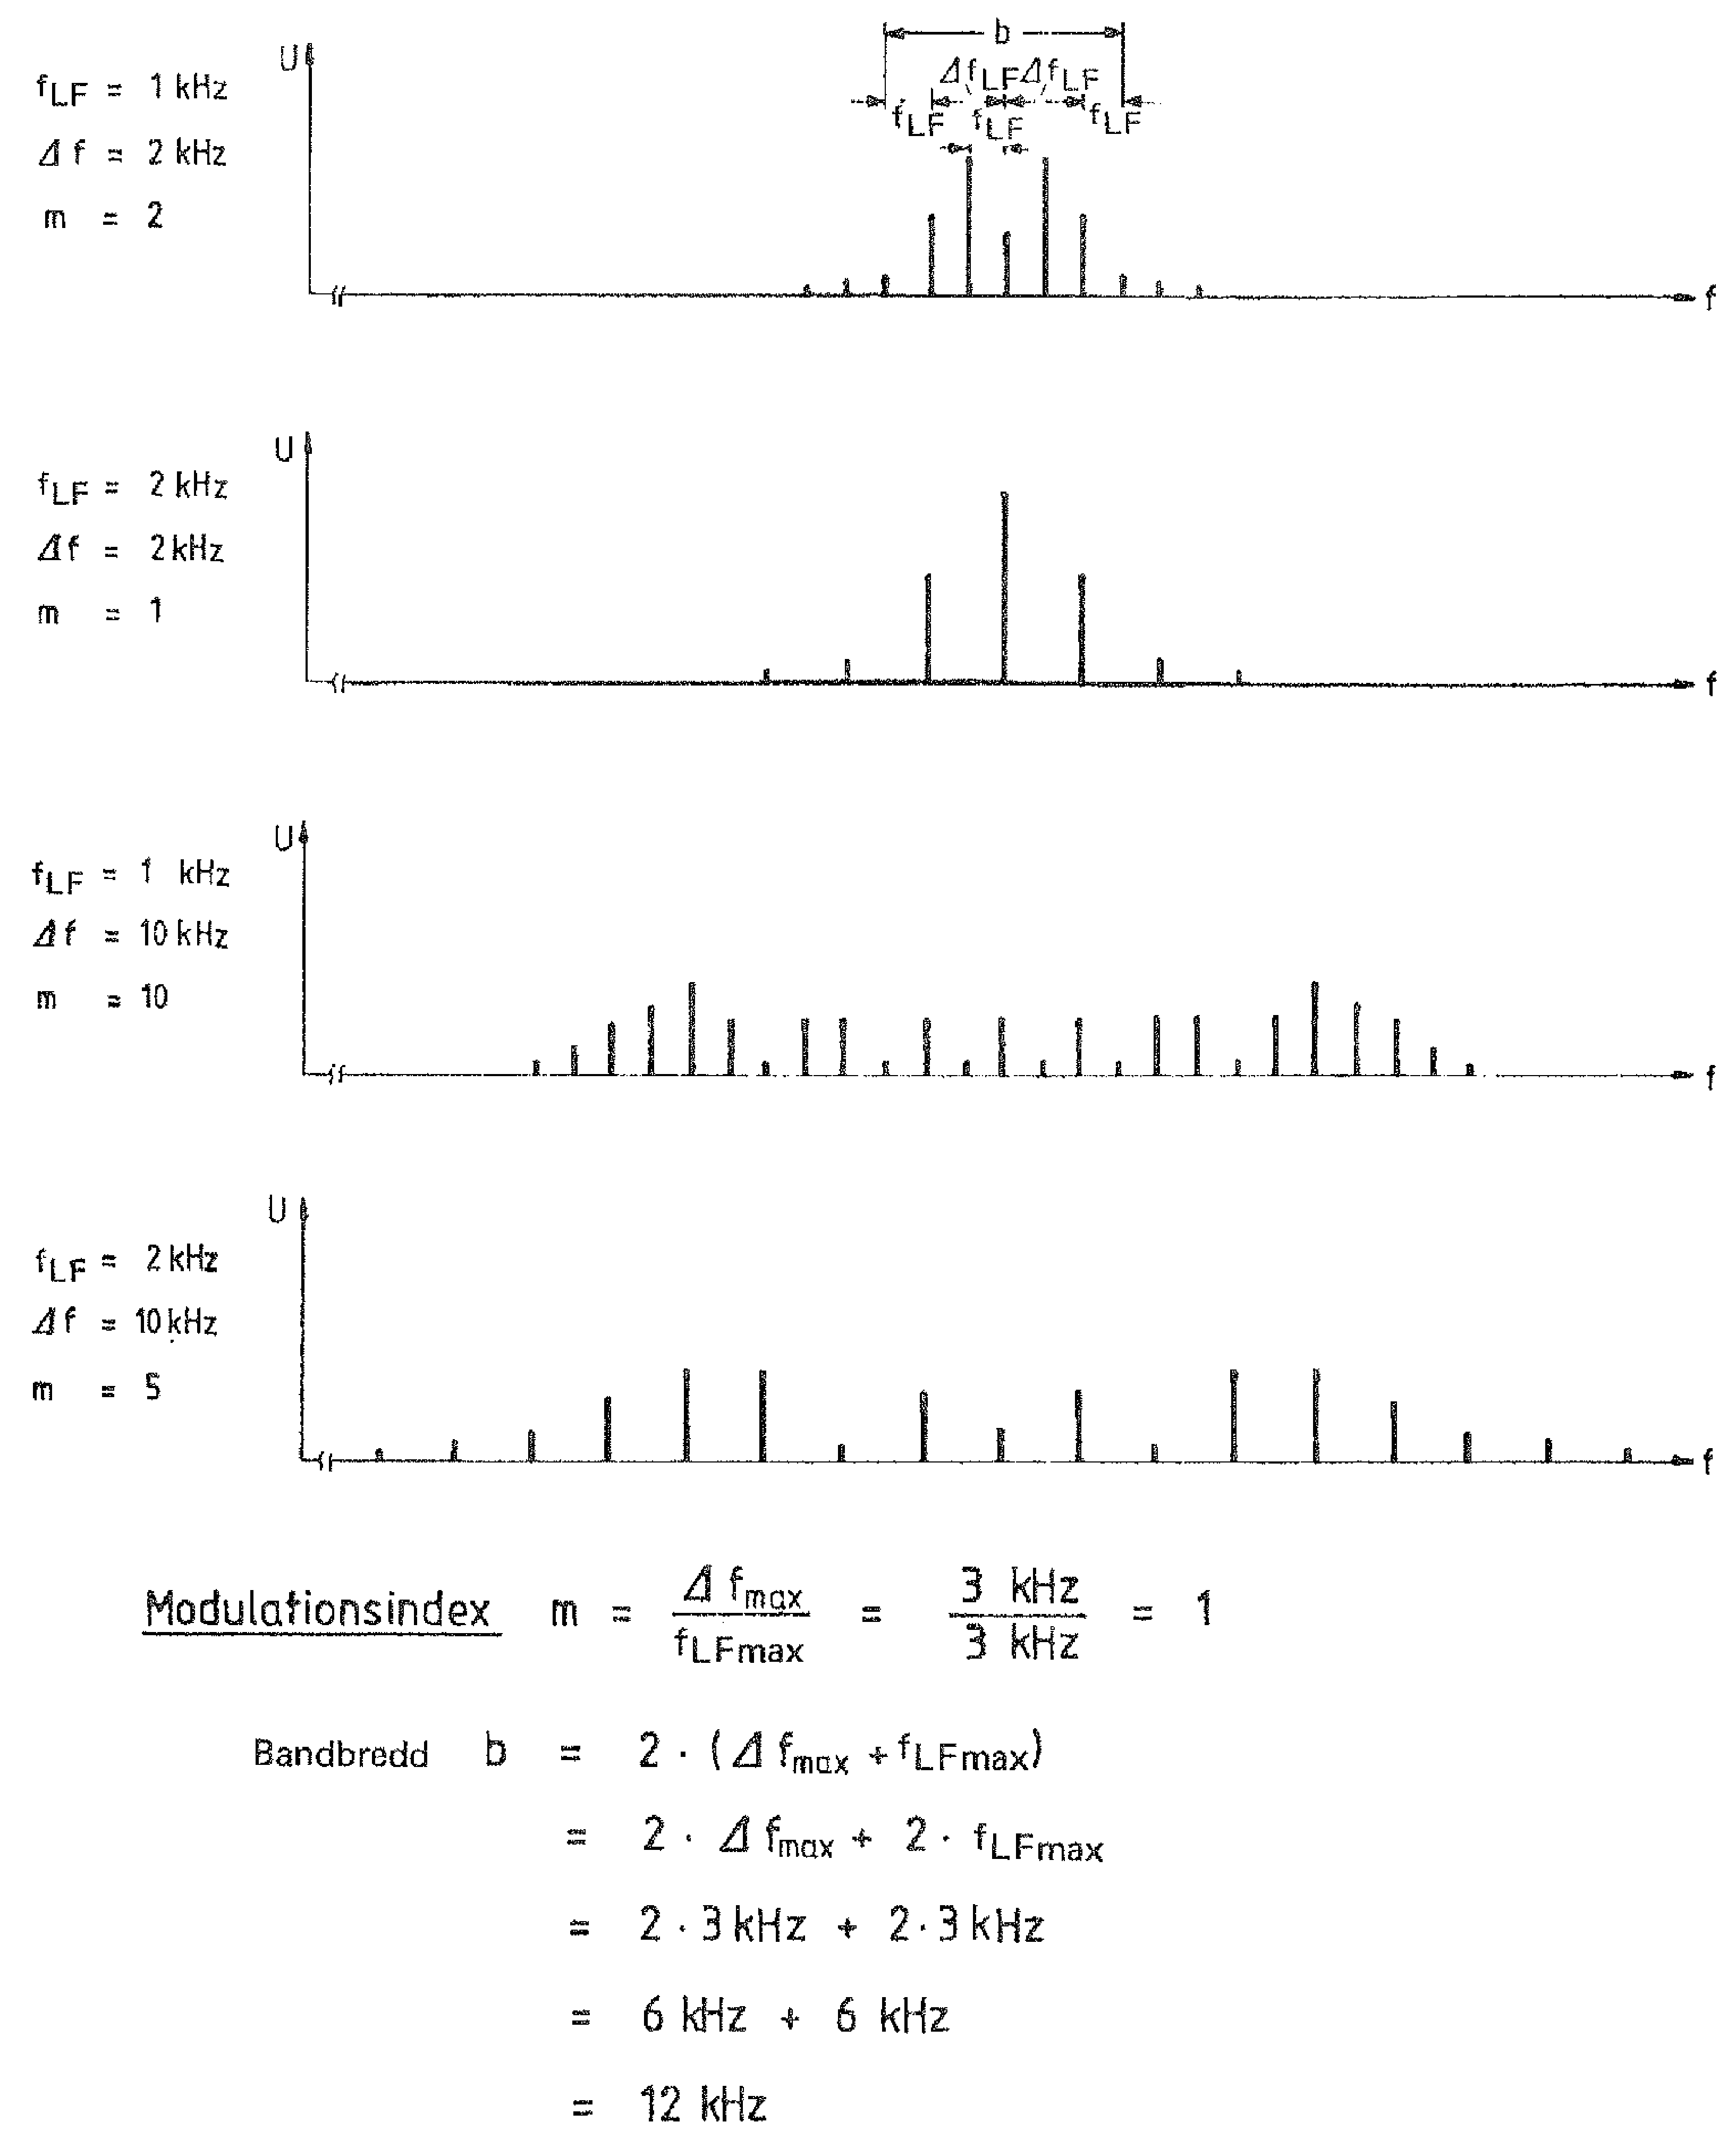
\includegraphics[width=\textwidth]{images/cropped_pdfs/bild_2_1-31.pdf}
\caption{Sidbandsspektrum vid FM-modulering med 1 sinuston}
\label{fig:BildII1-31}
\end{figure}

Bild \ref{fig:BildII1-31}.

Vid vinkelmodulation uppstår talrika sidofrekvenser, som beror av den
modulerande frekvensen \(f_{LF}\). Amplitudfördelningen mellan sidofrekvenserna
står i förhållande till deviationen, varvid deras amplitud blir mindre desto
längre bort från bärvågen de är.

I praktiken anses en sidofrekvens försumbar när dess amplitud är mindre än 1~\%
av amplituden för omodulerad bärvåg.

För beräkning av bandbredden används begreppet modulationsindex m, vilket är
kvoten av maximal deviation \(\Delta f\) och högsta frekvensen \(f_{LF}\).

\(m = \dfrac{\Delta f_{max}}{f_{LFmax}}\)

Inom amatörradion är det vanligt att arbeta med \(\Delta f_{max} = 3 kHz\) och
\(f_{LFmax} = 3 kHz\), d.v.s. \(m = 1\).

Vid modulationsindex \(m = 1\), gäller följande
formel för bandbredden \(b\)

\(b = 2 \cdot ( \Delta f_{max} + f_{LFmax}) = 2 \cdot \Delta f_{max}
 + 2 \cdot f_{LFmax}\)

Med ovan nämnda värden blir bandbredden \(b = 2 \cdot (3 kHz + 3 kHz)
 = 12 kHz\)

Bandbredden ökar således både med ökande deviation och ökande modulerande
frekvens. För att inte interferera med trafik på grannkanalerna måste såväl
deviation som frekvensen på den modulerande signalen begränsas. En
deviationsbegränsare begränsar amplituden på denna signal. Ett lågpassfilter
reducerar den distorsion, som uppstår av begränsningen. Vidare undertrycks
modulerande frekvenser högre än 3~kHz, vilket är tillräckligt för överföring
av tal.

\paragraph{Jämförelse}

En VHF-rundradiosändare är tilldelad ett större frekvensutrymme och kan därför
använda mycket större bandbredd.

Där är \(\Delta f_{max} = 75 kHz\) och \(f_{LFmax} =15 kHz\), därmed är
\(m = \frac{75}{15} = 5\) och \(b = 2 \cdot (75 + 15) = 180 kHz\).

Som framgår av tabellen på nästa uppslag varierar bärvågens liksom
sidofrekvensernas inbördes amplitud med modulationsindex. Detta ska jämföras
med AM där bärvågens amplitud är konstant och endast sidbandens amplitud
varierar.

Vid vinkelmodulation utsläcks bärvågen \(A_0\) vid modulationsindex 2.404. Den
blir sedan ''negativ'' vid högre index, vilket betyder att den återkommer, men
att dess fasläge blir omvänt. I vinkelmodulation tas energin i sidbanden från
bärvågen, vilket innebär att den totala effekten förblir densamma oavsett
modulationsindex.

\paragraph{Kännetecken för sändningsslaget F3E (FM)}
\index{F3E}

Fördelar: F3E-sändaren är enkel till sin uppbyggnad och hög överföringskvalitet
uppnås vid stor bandbredd, störningar från amplitudmodulerade signaler t.ex.
tändgnistor undertrycks i mottagaren.

Nackdelar: En relativt stor bandbredd behövs för överföring av ett basband med
stort frekvensomfång. Sändaren måste avge full effekt, även när modulation inte
sker.

\begin{table*}[h]
\begin{center}
\begin{tabular}{ll|l|l|l|l|l|l|l|l|}
\cline{3-9}
&\multicolumn{1}{l}{}  & \multicolumn{7}{|c|}{Modulationsindex} \\ \cline{3-9}
&\multicolumn{1}{l|}{}  &   1   &   2   &    3   &    4   &    5   &    6   &    7   \\ \hline
\multicolumn{1}{|c|}{\multirow{11}{*}{\rotatebox[origin=c]{90}{Relativ amplitud på}}}&\(A_0\) & 0,765 & 0,224 & -0,260 & -0,397 & -0,178 &  0,151 &  0,300 \\
\multicolumn{1}{|c|}{}&\(A_1\) & 0,440 & 0,577 &  0,334 & -0,066 & -0,328 & -0,277 & -0,005 \\
\multicolumn{1}{|c|}{}&\(A_2\) & 0,115 & 0,353 &  0,486 &  0,364 &  0,047 & -0,243 & -0,301 \\
\multicolumn{1}{|c|}{}&\(A_3\) & 0,020 & 0,129 &  0,309 &  0,430 &  0,365 &  0,115 & -0,168 \\
\multicolumn{1}{|c|}{}&\(A_4\) &       & 0,034 &  0,132 &  0,281 &  0,391 &  0,358 &  0,158 \\
\multicolumn{1}{|c|}{}&\(A_5\) &       & 0,016 &  0,043 &  0,132 &  0,261 &  0,362 &  0,348 \\
\multicolumn{1}{|c|}{}&\(A_6\) & \multicolumn{2}{c|}{} &  0,011 &  0,049 &  0,131 &  0,246 &  0,339 \\
\multicolumn{1}{|c|}{}&\(A_7\) & \multicolumn{3}{c|}{} &  0,015 &  0,053 &  0,130 &  0,234 \\
\multicolumn{1}{|c|}{}&\(A_8\) & \multicolumn{4}{c|}{}           &  0,018 &  0,057 &  0,128 \\
\multicolumn{1}{|c|}{}&\(A_9\) & \multicolumn{4}{c}{} &        &  0,021 &  0,059 \\
\multicolumn{1}{|c|}{}&\(A_{10}\) & \multicolumn{5}{c}{Tomma fält för \(A_n\) under 0,01 (1 \%)} &  &  0,024 \\ \hline
\end{tabular}
\end{center}
\caption{Relativa amplituden på bärvåg $A_0$ och sidofrekvenser $A_1$--$A_{10}$ vid
modulationsindex 1--7 (Vid omodulerad bärvåg är modulationsindex 0. Då är
bärvågens relativa amplitud 1,0)}
\end{table*}


\subsection{Fasmodulation (även kallat PM)}
\index{fasmodulation}
\index{PM}

Vid fasmodulation varierar bärvågens fasläge i förhållande till ett
referensvärde. Vid PM är frekvensändringen -- deviationen -- direkt proportionell
till hur snabbt fasläget på den modulerande frekvensen ändras och till den
totala fasändringen. Hastigheten på fasändringen är direkt proportionell till
frekvensen på den modulerande frekvensen och till den momentana amplituden på
den modulerande signalen.

Det betyder att deviationen i PM-system ökar både med den momentana amplituden
och frekvensen på den modulerande signalen. Detta att jämföras med FM-system där
deviationen är proportionell till den momentana amplituden på den modulerande
signalen.

I PM-system uppfattar demodulatorn i mottagaren endast momentana ändringar i
bärvågsfrekvensen. Till skillnad från vid FM, så kan därför ändringar i
likspänningsnivåer överföras endast om en fasreferens används.

Med konstant amplitud på insignalen till modulatorn, så är vid PM
modulationsindex konstant oavsett modulerande frekvens, medan vid FM
modulationsindex varierar med den modulerande frekvensen.

\subsection{Frekvens- och fasmodulation jämförs}

\begin{itemize}
\item Frekvensmodulation (FM) alstras genom att sändarens oscillatorfrekvens
varieras (devieras) i takt med den modulerande signalen (t.ex. tal). Det gör man
genom att variera resonansfrekvensen i den svängningskrets som styr
oscillatorfrekvensen.

\item Fasmodulation (PM) alstras vanligen genom att efter sändaroscillatorn
variera den modulerande signalens fasläge i förhållande till en omodulerad
bärvåg -- s.k. fasmodulering. Det gör man genom att variera resonansfrekvensen i
en svängningskrets efter oscillatorn- d.v.s. utan att påverka
oscillatorfrekvensen.

\item I båda fallen ändrar man alltså resonansfrekvensen i en svängningskrets i
takt med frekvensen i den modulerande spänningen, men att denna krets har olika
placering i FM-sändare respektive PM-sändare.

\item I sändaren alstras det i båda fallen utfrekvenser som devierar från
oscillatorns vilofrekvens. Graden av deviation skiljer emellertid vid FM och PM.
Vid FM är deviationen proportionell mot amplituden på den modulerande
underbärvågen medan deviationen vid PM är proportionell mot produkten av den
modulerande underbärvågens amplitud och frekvens.

\item Den hörbara skillnaden mellan FM och PM är därför en annorlunda
frekvensgång. Vid samtidig användning av PM-sändare och FM-mottagare är det
alltså lämpligt att justera frekvensgången i PM-sändarens modulator, lämpligen
med 6~dB dämpning per oktav ökad frekvens.
\end{itemize}

\subsection{Pulsmodulation}
\index{pulsmodulation}
\index{PWM}
\index{PAM}
\index{PPM}

Pulsmodulation används mest i mikrovågsområdet. Pulsmodulerade signaler sänds
vanligen som en serie korta pulser åtskilda av relativt långa pauser utan
modulering.

En typisk sändning kan bestå av pulser med en längd av 1 \(\mu\)s och en
frekvens av 1000~Hz. Toppeffekten på en pulssändning är därför mycket högre än
dess medeleffekt

Före WARC 79 var symbolen för all pulssändning P. Därefter används P endast för
omodulerade pulståg. Annan pulsmodulation har följande symboler

\begin{description}
\item[K] -- puls-/amplitudmodulation (PAM)
\item[L] -- pulsviddmodulation (PWM)
\item[M] -- pulsposition/fasmodulation (PPM)
\item[Q] -- vinkelmodulation under pulsen
\item[V] -- kombination av dessa eller annat sätt.
\end{description}

\begin{table*}[h]
\begin{center}
\begin{tabular}{|l|l|l|l|l|}
\hline
Sändningsslag & Amplituden på & Tonhöjden på & Bandbredden b      & För stor amplitud \\
              & LF-signalen   & LF-signalen  & förhåller sig till & på LF-signalen \\
              & påverkar      & påverkar     &                    & medför \\ \hline
A3E (AM) & amplituden i   & sidofrekvenser- & LF-signalens    & övermodulering \\
         & båda sidbanden & nas avstånd    & högsta frekvens & och för stor bandbredd \\
         &                & från bärvågen  & & \\
J3E (SSB)& amplituden på  & sidofrekvenser- & skillnaden mellan & för stor bandbredd,\\
         & utsänt sidband & nas avstånd    & LF-signalens      & överstyrning av\\
         &                & från bärvågen  & högsta och lägsta & förstärkarsteg\\
         &                &                & frekvens          & \\
F3E (FM) & deviationen    & hastigheten på & dubbla summan     & för stor deviation,\\
         &                & bärvågens      & av största devia- & för stor bandbredd\\
         &                & frekvens-      & tion och högsta   & \\
         &                & ändring        & LF-frekvens       & \\ \hline
\end{tabular}
\end{center}
\caption{Jämförelse mellan några vanliga sändningsslag inom amatörradio}
\end{table*}

\subsection{Digital modulationer}
\textbf{HAREC a.\ref{HAREC.a.1.8.8}\label{myHAREC.a.1.8.8}}
\index{digital modulation}

Utöver de klassiska analoga modulationsmetoder finns ett antal digitala
modulationsformer. De är anpassade för transmission av binär data. I viss mån
kan CW ses som digital modulation där en 0 moduleras utan bärvåg och 1 moduleras
med bärvåg. Det finns dock flera andra modulationsmetoder som FSK, 2-PSK/BPSK,
4-PSK och QAM som presenteras i följande delavsnitt.

\subsubsection{Frekvensskift modulation -- FSK}
\textbf{HAREC a.\ref{HAREC.a.1.8.8a}\label{myHAREC.a.1.8.8a}}
\index{frekvensskift modulation}
\index{Frequency Shift Keying (FSK)}
\index{FSK}
\index{frekvensmodulation}
\index{FM}
\index{GFSK}
\index{Gaussiskt filter}
\index{C4FM}
\index{JT65}
\index{JT9}

\emph{Frekvensskift modulation} (eng. \emph{Frequency Shift Keying (FSK)})
skiljer sig från CW modulationen med att den ändrar frekvensen, dvs. är en
variant av frekvensmodulation. I den enklaste formen, binär FSK, så växlar man
mellan 2 frekvenser, där en frekvens får representera 0 och den andra får
representera 1. Denna metod har används för modem på telefon-förbindelser,
så som Bell 103.

Eftersom varje växling mellan frekvenser ger avbrott i bägge signalerna,
likt nycklingen i CW, så kommer de skapa sidband. Av det skälet filtrerar man
gärna signalen, och använder man ett Gaussiskt filter får man Gaussian Frequency
Shift Keying (GFSK) som används av t.ex. GSM telefoni.

Man kan använda fler än 2 frekvenser, t.ex. används 4 frekvenser i Continuous
4 level FM (C4FM) i Phase 1 radios i Project 25 samt Fusion.

Frekvensskift används även för att sända långsamma meddelanden där JT65
använder 65 frekvenser den skiftar mellan, medans JT9 använder 9 frekvenser.

\subsubsection{Binär fasskift modulation -- 2-PSK \& BPSK}
\textbf{HAREC a.\ref{HAREC.a.1.8.8b}\label{myHAREC.a.1.8.8b}}
\index{binär fasskift modulation}
\index{fasskift modulation!binär}
\index{2-PSK}
\index{fasskift modulation!2-PSK}
\index{BPSK}
\index{fasskift modulation!BPSK}
\index{Costas loop}

Istället för att modulera frekvensen kan man modulera polariteten eller fasen.
En sådan modulationsform är \emph{binär fasskift modulation} (eng.
\emph{Binary Phase Shift Keying (BPSK)} eller \emph{2-state Phase Shift Keying
(2-PSK)}. Förenklat kan man säga att bärvågen moduleras med +1 eller -1,
ofta med +1 representerande 0 och -1 representerande 1.

En nackdel med BPSK är att blir polariteten förväxlad så kommer meddelandet
att bli inverterat, dvs. 0 blir 1 och 1 blir 0. BPSK behöver därför också
kompletteras med annan digital modulation för att hantera polariteten, något
som i allmänhet kan åstadkommas enkelt.

BPSK används t.ex. av satellitnavigationssystem som GPS, GLONASS och Galileo.
För att återvinna BPSK behöver man ofta en speciell variant av PLL-loop känd
som \emph{Costas loop}, eftersom en normal PLL-loop klarar inte av
teckenändringarna på signalen.

\subsubsection{Fyrnivå fasskiftmodulation -- 4-PSK}
\textbf{HAREC a.\ref{HAREC.a.1.8.8c}\label{myHAREC.a.1.8.8c}}
\index{4-PSK}
\index{fasskift modulation!4-PSK}
\index{kvadratur-modulering}
\index{quadrature modulation}
\index{in phase}
\index{quadrature}
\index{I/Q modulation}

Fasskiftmodulation kan även göras med flera nivåer, och 4 olika fas-lägen
kan användas och kallas då för \emph{fyrnivå fasskiftmodulation} (eng.
\emph{4-state Phase Shift Keying (4-PSK)}.

Istället för 180 graders fas-skift (0 och 180 grader) som 2-PSK/BPSK använder
så använder man 360/4 dvs. 90 graders fas-skift mellan symbolerna.
Ett effektivt sätt att avkoda det är att göra \emph{kvadratur-modulering}
(eng. \emph{quadrature modulation}) där man modulerar en signal till två
komponenter, i fas (eng. \emph{In Phase (I)}) och kvadratur (eng.
\emph{Quadrature (Q)}), ofta kallat I/Q modulering.

De fyra fas-lägena kan nu enkelt förklaras som amplituder i de olika fas-lägena
som anges av tabell \ref{tab:4-PSK}.

\begin{table*}[h]
\begin{center}
\begin{tabular}{|r|r|r|r|}
\hline
Symbol & Vinkel & I & Q \\ \hline
0 &   0 & +1 &  0 \\
1 &  90 &  0 & +1 \\
2 & 180 & -1 &  0 \\
3 & 270 &  0 & -1 \\ \hline
\end{tabular}
\end{center}
\caption{4-PSK i kvadratur-modulering}
\label{tab:4-PSK}
\end{table*}

Amplituden är densamma för alla 4 symbolerna, men med olika vinkel.
I likhet med 2-PSK/BPSK behöver man återvinna fasen och sedan kunna avgöra
vad som är 0 grader, men givet att det görs i den övriga modulationen så
kan informationen avkodas korrekt.

\subsubsection{Kvadratur-amplitud modulation -- QAM}
\textbf{HAREC a.\ref{HAREC.a.1.8.8d}\label{myHAREC.a.1.8.8d}}
\label{QAM}
\index{kvadratur-amplitud modulation}
\index{QAM}
\index{QAM-16}
\index{DAB}
\index{DVB-T}
\index{DVB-T2}
\index{Wi-Fi}

Medans fasskiftnings kan göras för fler fas-steg har man funnit att det är
inte lika smidigt för högre upplösningar. Redan vid 8 steg behöver man ha
I och Q värden som är \(\sqrt{1/2}\), vilket iofs går att approximera.
En smidigare modulationsform är istället att låta även amplituden variera,
och genom att låta några bitar modulera I och några bitar modulera Q så kan
man enkelt få en konsistent modulations-mappning som är effektiv att
implementera. Denna kallar man \emph{kvadratur-amplitud modulation} (eng.
\emph{Quadrature Amplitude Modulation (QAM)}).

Ofta benämner man olika varianter med antalet olika positioner, så att QAM-16
har 16 olika fas-amplitud-lägen. Ett exempel på hur QAM-16 kan moduleras finns
i tabell \ref{tab:QAM-16}.

\begin{table*}[h]
\begin{center}
\begin{tabular}{|r|r|r|r|r|r|r|}
\hline
Symbol & Isym & Qsym & Amplitud      & Vinkel &  I &   Q \\ \hline
     0 &    0 &    0 & \(3\sqrt{2}\) &    +45 & +3 &  +3 \\
     1 &    0 &    1 & \(\sqrt{10}\) &    +72 & +3 &  +1 \\
     2 &    0 &    2 & \(\sqrt{10}\) &   +108 & +3 &  -1 \\
     3 &    0 &    3 & \(3\sqrt{2}\) &   +135 & +3 &  -3 \\
     4 &    1 &    0 & \(\sqrt{10}\) &    +18 & +1 &  +3 \\
     5 &    1 &    1 &  \(\sqrt{2}\) &    +45 & +1 &  +1 \\
     6 &    1 &    2 &  \(\sqrt{2}\) &   +135 & +1 &  -1 \\
     7 &    1 &    3 & \(\sqrt{10}\) &   +162 & +1 &  -3 \\
     8 &    2 &    0 & \(\sqrt{10}\) &   +342 & -1 &  +3 \\
     9 &    2 &    1 &  \(\sqrt{2}\) &   +315 & -1 &  +1 \\
    10 &    2 &    2 &  \(\sqrt{2}\) &   +225 & -1 &  -1 \\
    11 &    2 &    3 & \(\sqrt{10}\) &   +198 & -1 &  -3 \\
    12 &    3 &    0 & \(3\sqrt{2}\) &   +225 & -3 &  +3 \\
    13 &    3 &    1 & \(\sqrt{10}\) &   +252 & -3 &  +1 \\
    14 &    3 &    2 & \(\sqrt{10}\) &   +288 & -3 &  -1 \\
    15 &    3 &    3 & \(3\sqrt{2}\) &   +315 & -3 &  -3 \\ \hline
\end{tabular}
\end{center}
\caption{Exempel på QAM-16 i kvadratur-modulering}
\label{tab:QAM-16}
\end{table*}

Medans både amplituder och vinklar kan kännas udda, så är det enkelt att
mappa bitarna över till I och Q amplituder via Isym och Qsym delarna av
symboler.

QAM-modulering används av DAB, DVB-T, DVB-T2, IEEE~802.11 (Wi-Fi),
mikrovågslänkar och många andra moderna system.
Mikrovågslänkar använder upp till QAM-2048.
En fördel med QAM-moduleringen är att det är enkelt att få samma avstånd
mellan de olika symbol-positionerna, och därmed kan också modulationen anpassas
till störningen. Detta nyttjas av många moderna modulations-system så att
QAM-modulationen anpassas utifrån mottagarens rapportering om störning.
Denna dynamiska anpassning gör att kommunikationen kan upprätthållas även om
kapaciteten tillåts variera.

\subsection{Digital modulation}
\textbf{HAREC a.\ref{HAREC.a.1.8.9}\label{myHAREC.a.1.8.9}}
\index{digital modulation}

Digital modulation innebär också att signalerna som sänds har lite andra
egenskaper än de analoga. Istället för varierande spänningsnivåer som för
t.ex. tal så skickar vi diskreta fixa nivåer, ofta i form av bitar. Det är
därför lämpligt att diskutera några grundläggande begrepp kring digital
modulation.

\subsubsection{Bit rate}
\textbf{HAREC a.\ref{HAREC.a.1.8.9a}\label{myHAREC.a.1.8.9a}}
\index{bit}
\index{byte}
\index{informationsmängd}
\index{informationsöverföringskapacitet}
\index{bit rate}

Informationen som vi skickar har vi kodat i bitar (eng. \emph{bit (b)}),
\emph{informationsmängden} vi har är därför ett visst antal bitar och takten på
denna informationsmängd blir därmed \emph{informationsöverföringskapaciteten}
(eng. \emph{bit rate}) i bitar per sekund.

Ofta brukar vi referera till informationsmängden i mängden \emph{byte (B)}
som t.ex. att en fil är 2~kB eller en bild är 1,25~MB. Då en byte innehåller
8 bitar, så motsvarar det 16~kb respektive 10~Mb. I dagligt tal pratar vi då om
storleken på en fil.

Överföringskapaciteten, eller i dagligt tal hastigheten, brukar vi ofta prata
om i termer av \emph{bit rate} som 10~Mb/s (ofta skrivet \emph{bps -- bits per
second}), dvs. man klarar av att överföra upp till 10 miljoner bitar per sekund.

Det är ofta som man pratar om den råa överföringskapaciteten, medans den
verkliga överföringskapaciteten för nyttotrafik är något lägre på grund av
olika former av packningsformat och protokoll-behov, så kallad \emph{overhead}.
Man ska därför vara noga med att skilja dessa åt.

\subsubsection{symboltakt -- Baud rate}
\textbf{HAREC a.\ref{HAREC.a.1.8.9b}\label{myHAREC.a.1.8.9b}}
\index{symbol}
\index{symboltakt}
\index{symbol rate}
\index{Baud rate}
\index{Emile Baudot}
\index{enheter!Baud (Bd)}

Som vi redan sett exempel på kan ibland bitar skickas en och en, eller
ihop-klumpade. Varje sådan ihop-klumpning kallas \emph{symbol}, och en symbol
kan bära en eller flera bitar, ibland inte ens ett jämnt antal.

Om man kan artikulera något i 2 olika \emph{nivåer} (av amplitud, fas, frekvens
eller kombination), så kan man representera 1 bit. Om man kan artikulera något
i 4 olika nivåer, så kan man representera 2 bitar. På samma sätt ger 8 nivåer
support för 3 bitar. Varje representation kallar man en symbol, och varje
symbol-tillfälle bär alltså 1, 2 eller 3 bitar information. Strikt räknat
är det logaritmen med bas 2 (2-logaritm eller $\log_{2}$) av antalet nivåer som
anger antalet bitar som en symbol kan bära. 3 nivåer brukar sägas kunna bära
1,5 bitar, vilket är en slarvig approximation men visar principen.

Den takt varmed symboler överförs, \emph{symbol-takten} (eng. \emph{symbol rate})
benämns även \emph{Baud rate}, efter Emile Baudot, med enheten \emph{Baud (Bd)}.
Enheten Baud (förkortat Bd) anger antalet symboler per sekund. Genom att
multiplicera antalet symboler per sekund med antalet bitar per symbol fås
överföringskapaciteten bitar per sekund.

\subsubsection{Bandbredd}
\textbf{HAREC a.\ref{HAREC.a.1.8.9c}\label{myHAREC.a.1.8.9c}}
\index{bandbredd}
\index{Nyqvist-teoremet}

Genom att justera antalet bitar per symbol så kan man ändra antalet symboler
per sekund utan att ändra överföringskapaciteten. En anledning till att man
vill göra det är för att bandbredden som används av en överföring är ungefär
proportionerlig med symboltakten, dvs. hur många Baud man överför i.
Detta påverkar hur stor del av radiospektrat man upptar, och därmed också hur
nära en annan signal man kan ligga i spektrat utan att störa varandra, dvs.
det påverkar frekvensplaneringen av bandet ifråga.

Ofta används begreppen bandbredd synonymt med överföringskapaciteten, eftersom
det finns en proportionell relation dem emellan, men bandbredden är inte den
enda parametern som krävs, så i mer strikta sammanhang ska dessa begrepp
hanteras som separata för att undvika missförstånd.

Bandbredden för en digital ström är besläktad med Nyquist-teoremet, som säger
att sample-raten måste vara minst dubbelt så hög som högsta frekvensen som
överförs.

\subsection{Bitfel -- detektion och korrigering}

Fram tills nu har vi diskuterat digital modulation utan att ta hänsyn till
störningar och hur dessa störningar påverkar vårt överförda data. Precis som
vår CW eller SSB kan vara störd av atmosfäriska störningar, andra sändare
eller helt enkelt vara svaga signaler så att det interna bruset blir en
begränsning, så kommer mottagningen av digitala signaler att bli störd.
Vi ska titta på dessa grundläggande begrepp som bitfel, bitfelssannolikhet,
felupptäckt samt korrigering med återsändning eller korrigeringskoder.

\subsubsection{Bitfel}
\index{bitfel}
\index{bit error}

Utan att gå inpå varför, så varje gång vi får fel så kommer en eller flera
bitar att bli fel, vi kallar varje sådant fel för att \emph{bitfel} (eng.
\emph{bit error}). Störningar kan göra att vi tolkar en symbol fel, det kan
resultera i att en eller flera bitar från den symbolen är fel.

Om vi i t.ex. QAM-16 koden i kapitel \ref{QAM} får in +0.2 i I och +1.1 i Q
så ser vi i tabell \ref{tab:QAM-16} att närmsta symbolen är symbol 5 med +1 i I
och +1 i Q. Vi skulle kunna anta att om I är större än 0 och mindre än 2, samt
Q är större än 0 och mindre än 2 så är symbol 5 den enda vettiga symbolen, och
det är precis den tolkning vi i allmänhet gör, för det är den symbolen vars
avstånd är lägst och därmed rimligast. Det kan dock vara så att man egentligen
sände symbol 9 med -1 i I och +1 i Q, och därmed fått för stor störning på I
för att man ska tolka det som rätt symbol. Vi kommer då lägga ut 9 istället
för 5, vilket innebär att två bitar har ändrats.

Genom att granska tabell \ref{tab:QAM-16} vidare så ser man att värdena för
I och Q för de olika symbolerna är gjord sådan att minsta avstånd är 2 mellan
alla närliggande symboler, i respektive I och Q riktning. Det förenklar
tolkning av symbolerna. Är dock störningen större än 1 i någon riktning så
kommer man tolka den symbolen fel, och det kan då leda till 1 eller fler
bit-fel.

\subsubsection{Bitfelssannolikhet}
\index{bitfelssannolikhet}
\index{bit error rate (BER)}
\index{BER}
\index{gaussiskt brus}
\index{brus!gaussiskt}
\index{gaussian noise}
\index{effektiv-värde}
\index{Root Mean Square (RMS)}
\index{RMS}
\index{Error Function (erf)}
\index{erf}

Om vi antar att vi inte har störning från några andra signaler, utan enbart har
brus som störning, så kan vi estimera \emph{bitfelssannolikheten} (eng.
\emph{bit error rate (BER)} ur hur starkt bruset är i förhållande till vårt
steg. Eftersom bruset antas vara vitt brus, så har det egenskaperna av
\emph{Gaussiskt brus} (eng. \emph{Gaussian noise}).

Gaussiskt brus har en statistisk fördelning med hög sannolikhet nära
medelvärdet, och avtar sedan med avståndet. Sannolikheten att man tolkar en
signal som vara på ena eller andra sidan av en gräns, beror på hur långt bort
från medelvärdet den gränsen, ofta benämnd kvantiserings-gränsen, är, i
förhållande till den effektiva värdet (eng. \emph{Root Mean Square (RMS)} är i
amplitud hos bruset. Detta kan uttryckas i form av den matematiska funktionen
\emph{error function (erf)}.

När gränsen är 1 sigma, dvs. 1 gånger RMS-värdet för brus-amplituden, från
medelvärdet så är 67~\% sannolikhet att värdet är i inom gränsvärdet, dvs. en
bitfelssannolikhet på 33~\%.
Ligger det inom 2 sigma, så har sannolikheten ökat till 97~\%, en
bitfelssannolikhet på 3~\% och vid 3 sigma är den 99,7~\% med en
bitfelssannolikhet på ringa 0,3~\%, vilket ofta används för många
ingenjörsapplikationer. Dock, för överföring av information har vi högre krav.
För en bitfelssannolikhet på \(10^{-12}\), ofta benämnt BER på 1E-12, så
behövs det 14 sigma bort till gränsen, dvs. brusmängden får max vara 1/14 av
kvantiseringsgränsen. Den råa radio-kanalen uppvisar dock sällan så bra
egenskaper, men det kan uppnås i kabel och fiber.

\subsubsection{Detektion}
\textbf{HAREC a.\ref{HAREC.a.1.8.10a}\label{myHAREC.a.1.8.10a}}
\index{bitfelsdetektion}
\index{paritet}
\index{CRC}

Eftersom störningar förekommer och man har behov av lägre bitfelssannolikhet
än vad den råa kanalen medger är det lämpligt att identifiera när det har
blivit bitfel. Detta kan utföras på många sätt, men ett sätt är att räkna fram
checksummor som skickas med datat. Det kräver visserligen en del av
informationsöverföringskapaciteten, men tjänsten det medger är att försäkra sig
om att informationen är rimligt korrekt.

En enkel form av checksumma är paritet, där bitarna i ett ord har summerats ihop
binärt (med XOR) för att bilda en checksumma. I mottagaränden görs samma
kombination och sedan jämförs det med paritetsbiten, och om de överensstämmer så
har inget bitfel upptäckts. Denna enkla metod har en svaghet i att ett jämnt
antal bitfel kommer att kompensera varandra, varvid det döljer bitfel från
upptäckt. Det är med andra ord inte en särdeles stark checksumma. Paritet
används t.ex. i seriekommunikation så som RS-232.

Ett flertal checksummor finns, för olika ändamål, olika mängd fel och olika
typer av fel. För lite större meddelanden är det vanligt att summera bytes
till en checksumma antingen additivt eller med XOR. För större meddelanden
används en lite mer intrikat metod som heter Cyclic Redundancy Check (CRC)
där man återmatar överskjutande del på checksumman till sig själv och får en
starkare kod den vägen. CRC används t.ex. i Ethernet.

\subsubsection{Omsändning}
\textbf{HAREC a.\ref{HAREC.a.1.8.10b}\label{myHAREC.a.1.8.10b}}
\index{omsändning}
\index{ARQ}
\index{TCP}

En enkel åtgärd för att hantera när man konstaterat att ett block data man
tagit emot har fel, är att begära omsändning. Genom att sändaren håller en
buffert med meddelanden som den skickat, och mottagaren meddelar sändare om
den mottagit meddelandet eller behöver ha det omskickat, så kan omsändning
realiseras. Automatisk omsändningsbegäran (eng. \emph{Automatic Repeat reQuest
(ARQ)}) är en typ av protokoll som gör automatisk omsändingsbegäran om ett
enskilt datablock, även kallat paket, inte kommit fram rätt eller helt
försvunnit. Ett sådant protokoll är TCP, som ingår i internet-sviten av TCP/IP
protokoll.

\subsubsection{Korrigeringskod -- FEC}
\textbf{HAREC a.\ref{HAREC.a.1.8.10c}\label{myHAREC.a.1.8.10c}}
\index{korrigeringskod}
\index{felrättandekod}
\index{FEC}
\index{AMTOR}
\index{Hamming-koder}
\index{paritet}
\index{Reed-Solomon (RS)}

En annan form av korrigering är att helt enkelt skicka för mycket data redan
från början, som mottagaren kan använda för att korrigera meddelandet utan att
skicka någon begäran till sändaren. Detta är praktiskt antingen om det skulle
ta för mycket tid eller om det helt enkelt inte finns någon kommunikation från
mottagaren till sändaren, t.ex. för satellit-mottagare.

En enkel form av felrättande kod används i AMTOR FEC, där man helt enkelt
sänder samma tecken två gånger. Liknande används i Bluetooth där meddelandet
sänds tre gånger, varvid man kan göra majoritets-röstning.

Andra system för FEC är Hamming-koder, paritets-paket, Reed-Solomon (RS) osv.

\section{Effekt och energi}
\textbf{HAREC a.\ref{HAREC.a.1.9}\label{myHAREC.a.1.9}}
\label{effect och energi}
\index{effekt}
\index{energi}

\subsection{Effekt i en sinusformad signal}
\textbf{HAREC a.\ref{HAREC.a.1.9.1}\label{myHAREC.a.1.9.1}}

För beräkning av effekten av en sinusformad signal använder man effektivvärdet
av spänning och ström.

\(U_{eff} = \dfrac{U_{max}}{\sqrt{2}}\) och \(I_{eff} = \dfrac{I_{max}}{\sqrt{2}}\)

\(P = U_{eff} \cdot I_{eff}\)

\subsection{Effektändring uttryckt i dB}
\textbf{HAREC a.\ref{HAREC.a.1.9.2}\label{myHAREC.a.1.9.2}}
\index{dB}
\index{dB!effekt}
\index{effekt!dB}

Måtten i det metriska systemet är alldagliga och ingen finner det märkligt att
det t. ex. går tio decimeter på en meter. Däremot är begreppet decibel ovant för
många.

I detta avsnitt förklaras det mycket användbara begreppet decibel. Decibel (dB)
är en tiondedel av grundenheten Bel (B).

Räkning med decibel grundas på logaritmer, som är ett bekvämt sätt att uttrycka
och behandla talvärden.

\begin{quote}\emph{
Decibel är ett dimensionslöst uttryck för graden av dämpning alternativt
förstärkning.
}\end{quote}

\emph{Effektdämpning} är följden av att vissa komponenter bromsar elektrisk ström. Den
bromsande faktorn kan vara en resistans R, induktans L, kapacitans C eller
sammansatta nätverk av R, L och C.

\emph{Effektförstärkning} innebär att en transistor, ett elektronrör eller annan s.k.
aktiv komponent kan styra en större elektrisk ström och därmed större effekt än
den själv styrs med. Vad som förorsakar effektförändringarna går vi inte in på i
detta sammanhang, utan byggdelarna betraktas som ''svarta lådor'' med
anslutningsklämmor.

En byggdel med två ingångs- och två utgångsklämmor kallas för ''fyrpol''.

\begin{figure}[th]
\begin{center}
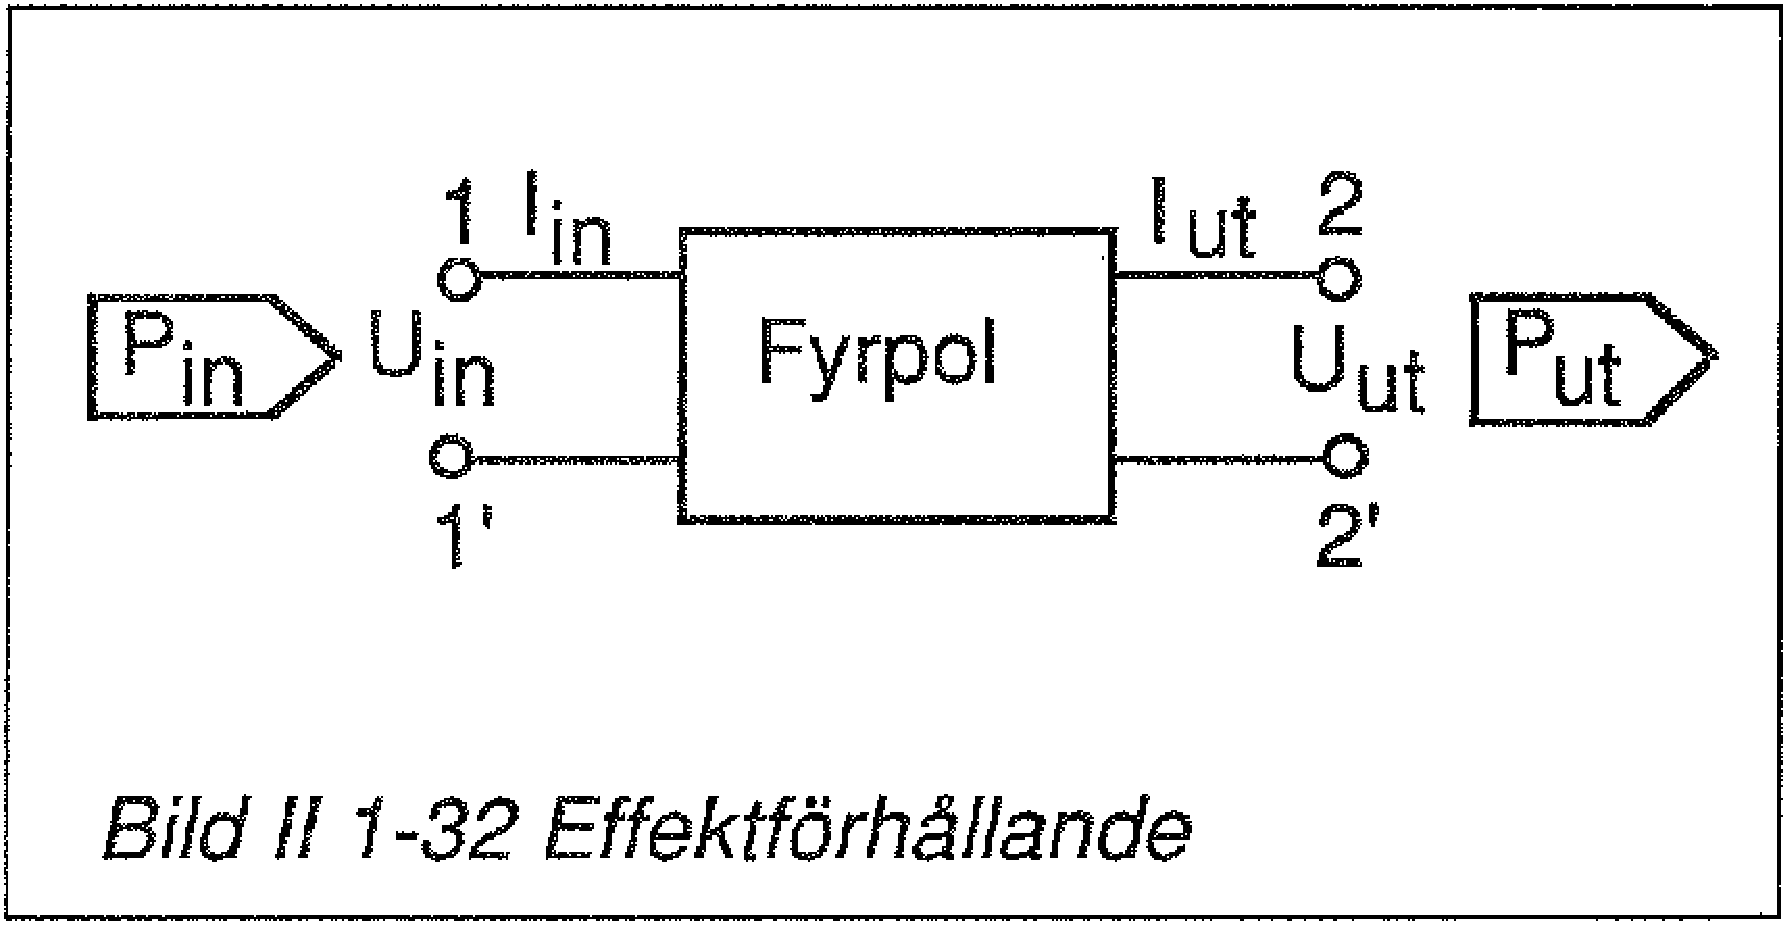
\includegraphics[width=7cm]{images/bild_2_1-32}
\caption{Effektförhållande}
\label{fig:BildII1-32}
\end{center}
\end{figure}

Antag att den inmatade effekten P är 1 W. Om effekten inte ändras vid passagen
genom fyrpolen, så är även den uttagna effekten 1 W.

\emph{Effektförhållandet} mellan in- och utgångarna är då

\(\dfrac{P_{in}}{P_{ut}} = \dfrac{1\ watt}{1\ watt} = 1 (kvoten = 1)\)

Oförändrad effekt varken dämpas eller förstärks, varför både dämpningen och
förstärkningen har talvärdet 0. Enheten på talvärdet är Bel, dämpningen eller
förstärkningen är således 0 Bel. En tiondel därav är 0~decibel (0 dB).

Omräkning av kvoten av en effektändring till dB görs så, att 10-logaritmen för
kvoten söks och resultatet blir effektändringen uttryckt i Bel (B). Om
resultatet uttrycks i dB, ska Bel-värdet multipliceras med 10.

Logaritmer förklaras i appendix \ref{logaritmer}.

För att förenkla beräkningen av dB-talet divideras det högre effekttalet med det
lägre. Bokstaven a i följande formler betyder antingen förstärkning (+a) eller
dämpning (-a) beroendet på vilket förtecken som sätts.

\(a[B] = \log \dfrac{P_\text{hög}}{P_\text{låg}}\)

\(a[dB] = 10\log \dfrac{P_\text{hög}}{P_\text{låg}}\)

Att addera eller subtrahera värden på en logaritmisk skala, motsvarar att
multiplicera resp. dividera värden på en linjär skala. Huvudskalorna på en
räknesticka är logaritmiska. (Räknestickan är ett enkelt, förut mycket använt
hjälpmedel).

Med hjälp av nomogrammet i bild \ref{ellära-nomogram-db-effekt} kan en \textbf{effektändring}, uttryckt som kvot
(effekterna dividerade med varandra), omvandlas till decibel och omvänt.

\begin{figure}
  \fbox{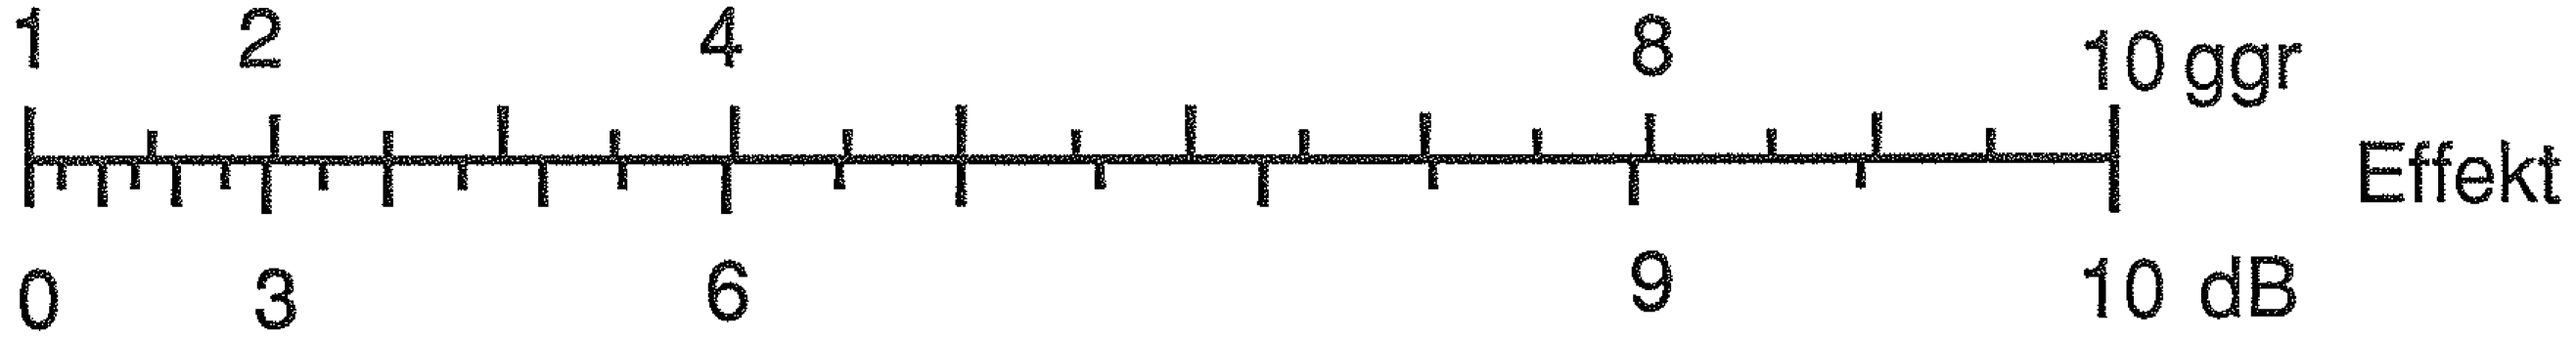
\includegraphics[width=\textwidth]{images/nomogram_db_effekt}}
  \caption{Nomogram för omvandling mellan effekt och decibel}
  \label{ellära-nomogram-db-effekt}
\end{figure}

Följande avrundade värden kan utläsas:

\begin{tabular}{rlrlrl}
0 dB & = 1 &  1 dB & =  1,25 & 2 dB = 1,6 \\
3 dB & = 2 &  4 dB & =  2,5  & 5 dB = 3,2 \\
6 dB & = 4 &  7 dB & =  5    & 8 dB = 6,3 \\
9 dB & = 8 & 10 dB & = 10    & 11 dB = 12,5
\end{tabular}

\begin{quote}\emph{
d.v.s. vid ökning fördubblas effekten för var 3:e dB och vid minskning
halveras effekten för var 3:e dB.
}\end{quote}

Om kvoten är en eller flera 10-potenser högre än 10, så kan nomogrammet utökas
enligt följande tabell.

\begin{tabular}{rllr}
Kvot av & Analys             & Skriv            & dB \\
\(P_\text{hög}/P_\text{låg}\) &          &                  &    \\
     1 & 1 har 0 nollor      & \(0 \cdot 10\) = &  0 \\
    10 & 10 har 1 nolla      & \(1 \cdot 10\) = & 10 \\
   100 & 100 har 2 nollor    & \(2 \cdot 10\) = & 20 \\
 1 000 &  1 000 har 3 nollor & \(3 \cdot 10\) = & 30 \\
10 000 & 10 000 har 4 nollor & \(4 \cdot 10\) = & 40
\end{tabular}

\subsection{Strömändring uttryckt i dB}
\index{ström!dB}
\index{dB!ström}

Förhållandet mellan strömmar liksom mellan spänningar kan även uttryckas i dB,
men annorlunda än mellan effekter. En fyrpol med inbördes lika ingångs- och utgångsimpedans är förutsättningen för jämförelse.

Enligt Joules lag är \(P = I^2 \cdot R\) (\(P = U \cdot I\))

således \(\dfrac{P_\text{h{\oe}g}}{P_\text{l{\aa}g}} = \dfrac{I_\text{hög}^2 \cdot R}{I_\text{l{\aa}g}^2 \cdot R}\)

R kan avkortas \emph{om in- och utgångsimpedanserna (resistanserna) är lika}.

En jämförelse uttryckt i dB kan endast göras
under samma förutsättningar; här att impedanserna (resistanserna) är lika,

således \(\dfrac{P_\text{hög}}{P_\text{låg}} = \dfrac{I_\text{hög}^2}{I_\text{låg}^2}\)

Effektförhållandet eller kvadratvärdet på
strömförhållandet kan uttryckas logaritmiskt
i B eller dB

\(a[dB] = 10\log \dfrac{I_\text{hög}^2}{I_\text{låg}^2}\)

Eftersom \(\log x^2 = 2 \cdot \log x\), fås slutligen

\(a[dB] = 20\log \dfrac{I_\text{hög}}{I_\text{låg}}\)

\subsection{Spänningsändring uttryckt i dB}
\index{spänning!dB}
\index{dB!spänning}

Förhållandet mellan spänningar kan uttryckas i dB på ett liknande sätt som med
strömmar.

Enligt Joules lag är \(P = \frac{U^2}{R}\) (\(P = U \cdot I\))

Två effekter kan ställas i förhållande till varandra på följande sätt:

\(\dfrac{P_\text{hög}}{P_\text{låg}}=\dfrac{U_\text{hög}^2 \cdot R}{U_\text{låg}^2 \cdot R}\)

R avkortas och efter omskrivning fås en formel som liknar den för strömmar

\(\dfrac{P_\text{hög}}{P_\text{låg}} = \dfrac{U_\text{hög}^2}{U_\text{låg}^2}\)

\(a[dB] = 20\log \dfrac{U_\text{hög}}{U_\text{låg}}\)

Med nomogrammet i bild \ref{ellära-nomogram-db-spänning} kan kvoten av en ström- eller spänningsändring omvandlas
till decibel och tvärt om.

\begin{figure}
  \fbox{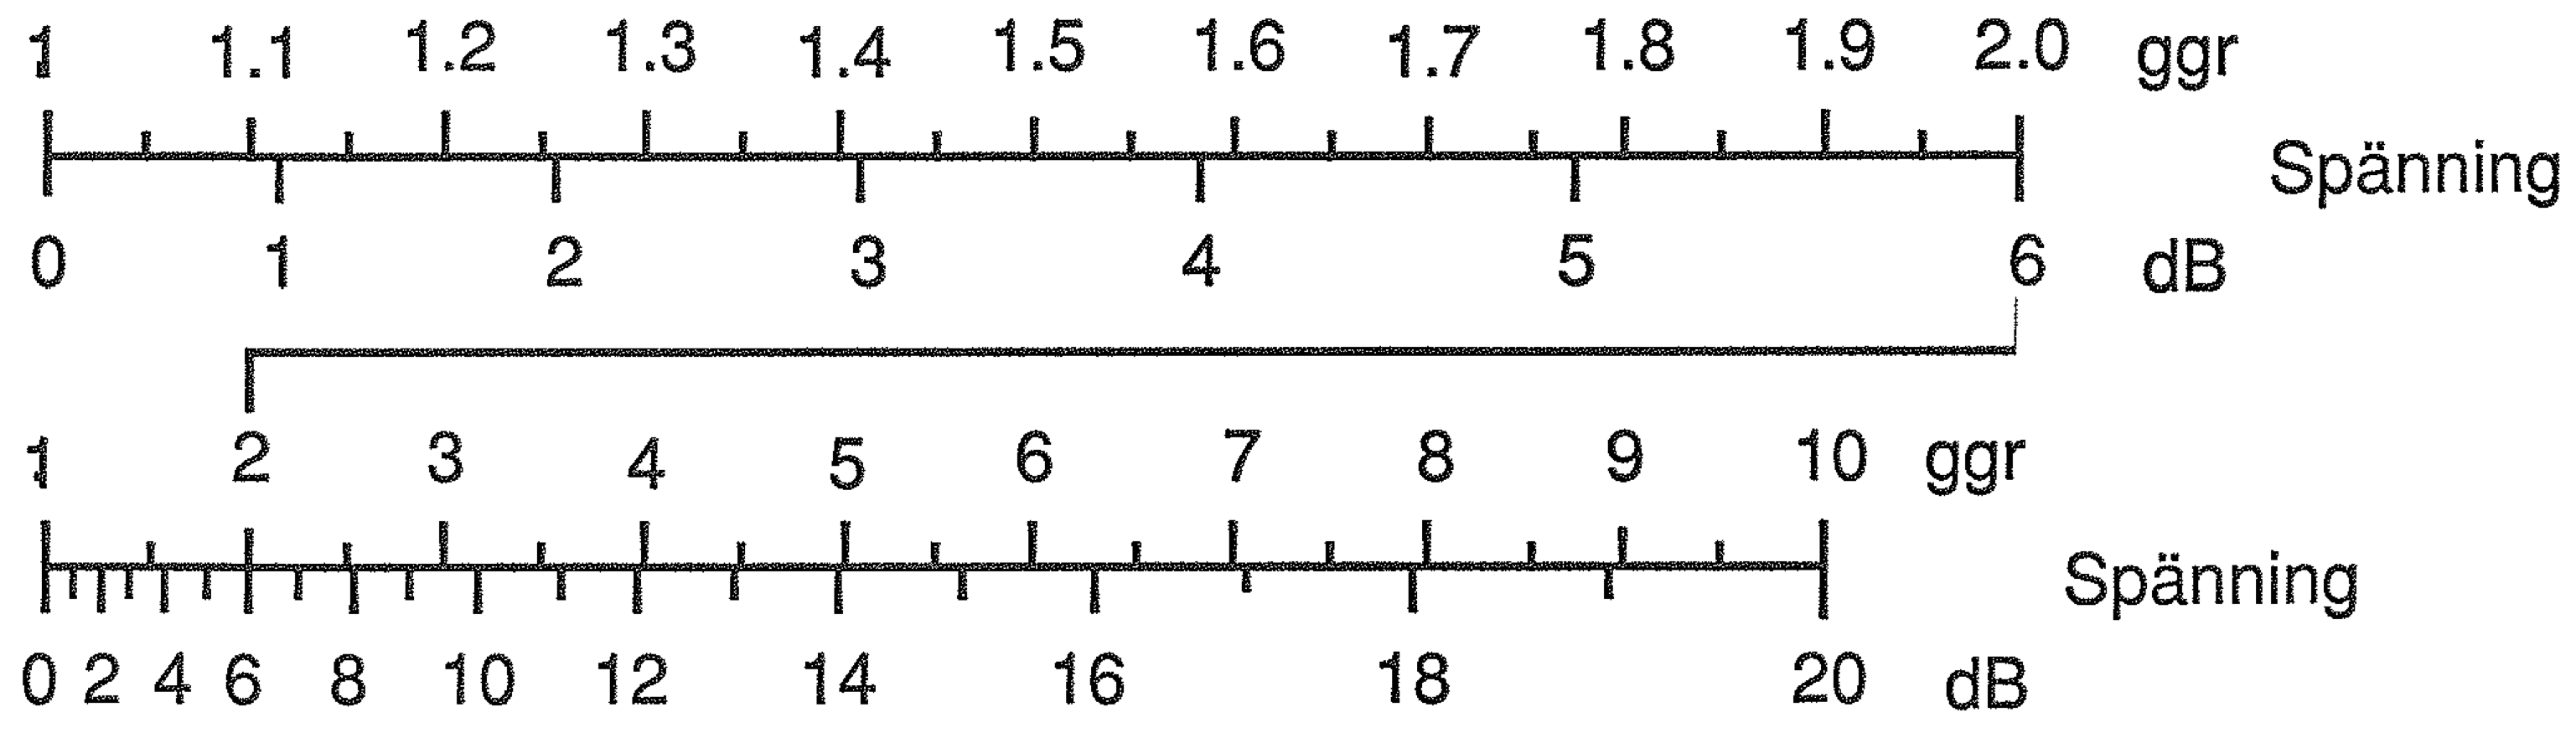
\includegraphics[width=\textwidth]{images/nomogram_db_spanning}}
  \caption{Nomogram för omvandling mellan spänning och decibel}
  \label{ellära-nomogram-db-spänning}
\end{figure}

Följande avrundade värden kan utläsas:

\begin{tabular}{rlrlrl}
0 dB & = 1   &  1 dB & = 1,12 &  2 dB = 1,25 \\
3 dB & = 1,4 &  4 dB & = 1,6  &  5 dB = 1,8 \\
6 dB & = 2   &  7 dB & = 2,24 &  8 dB = 2,5 \\
9 dB & = 2,8 & 10 dB & = 3,2  & 11 dB = 3,6
\end{tabular}

\begin{quote}\emph{
d. v. s. vid ökning fördubblas strömmen resp. spänningen för var 6:e dB och att
vid minskning halveras strömmen resp. spänningen för var 6:e dB.
}\end{quote}

Om kvoten är en eller flera 10-potenser högre än 10, så kan nomogrammet utökas
enligt följande tabell.

\begin{tabular}{rllr}
Kvot av & Analys             & Skriv            & dB \\
\(U_\text{hög}/U_\text{låg}\) &          &                  &    \\
\(I_\text{hög}/I_\text{låg}\) &          &                  &    \\
     1 & 1 har 0 nollor      & \(0 \cdot 20\) = &  0 \\
    10 & 10 har 1 nolla      & \(1 \cdot 20\) = & 20 \\
   100 & 100 har 2 nollor    & \(2 \cdot 20\) = & 40 \\
 1 000 &  1 000 har 3 nollor & \(3 \cdot 20\) = & 60 \\
10 000 & 10 000 har 4 nollor & \(4 \cdot 20\) = & 80
\end{tabular}

Se appendix \ref{decibel} för beräkning med tabeller.

\subsection{Ändring uttryckt i dB vid förstärkande eller dämpande anordningar kopplade i serie}
\textbf{HAREC a.\ref{HAREC.a.1.9.3}\label{myHAREC.a.1.9.3}}

Ett räkneexempel på effektändringar:
Fråga:
Vi har en enkel sändaranläggning med ett drivsteg med en in effekt av 10 W.
Drivsteget förstärker med 6 dB. Vidare har vi ett effektslutsteg som förstärker
med 10 dB. Antennkabeln dämpar med 1 dB.

Med vilken effekt matas själva antennen?

Svar: (två sätt att lösa uppgiften)
\begin{enumerate}
\item Drivsteget förstärker fyra gånger, slutsteget förstärker tio gånger och
kabeln dämpar \(1/1,25 = 0,8\) gånger. Antennen matas då med
\(10 \cdot 4 \cdot 10 \cdot 0,8 = 320\ W\).
\item Drivstegets 6 dB plus slutstegets 10 dB minus antennkabelns 1 dB = 15 dB.
15 dB är \(10 + 5\ dB\) d.v.s. \(10 \cdot 3,2 = 32\ ggr\). Antennen matas med
\(10\ W \cdot 32 = 320\ W\).
\end{enumerate}

\subsection{Impedansanpassning}
\textbf{HAREC a.\ref{HAREC.a.1.9.4}\label{myHAREC.a.1.9.4}}
\index{impedansanpassning}
\index{impedans!anpassning}

Impedansanpassning är av stor betydelse inom kommunikationstekniken.
Normalt vill man nämligen överföra mesta möjliga effekt från energikällan
(t.ex. sändaren) till förbrukaren (t.ex. antennen).

Varje spänningskälla har en inre resistans \(R_i\). Det innebär som först att
källan inte kan avge oändligt stor ström. För att förenkla det hela antar vi nu
att en sändare med den inre resistansen \(R_i\) ansluts direkt till en antenn
med resistansen \(R_a\).

Målet med anpassningen är att finna det optimala förhållandet mellan
sändarresistansen och antennresistansen för att kunna överföra maximal effekt.
Vi har de två ytterlighetsfallen obelastad sändare respektive kortsluten
sändare. Sändarens elektromotoriska kraft (EMK) betecknas som \(E\ [V]\) och
sändarens utspänning som \(U\ [V]\).

Fall 1.
En obelastad sändare avger ingen ström när ingen antenn eller en med oändligt
stor resistans har anslutits.
Alltså vid obelastad sändare:

\(
\begin{array}{lllll}
R_a = \infty & & I = 0 & & U = E
\end{array}
\)

Fall 2.
När sändarutgången är kortsluten, d.v.s. belastningen (antennresistansen) är
noll ohm, avger sändaren en ström som beror av EMK och inre resistans. Eftersom
sändarutgången är kortsluten är utspänningen \(U\) noll.
Alltså vid kortsluten sändare:

\(
\begin{array}{lllll}
R_a = 0 & & I = \dfrac{E}{R_i} & & U = O
\end{array}
\)

I båda ytterlighetsfallen är den effekt som omsätts i \(R_a\) lika med noll.
För att få ut någon effekt måste man alltså söka ett värde på \(R_a\) som
ligger mellan ytterlighetsvärdena.

Enligt formeln för spänningsdelare är utspänningen

\(U = E \cdot \dfrac{R_a}{R_a+R_i}\)

Formeln för uteffektens effektivvärde är

\(P_{ut} = \dfrac{U^2}{R_a}\)

Efter insättning får man

\(P_{ut} = \dfrac{E^2 \cdot R_a}{(R_a + R_i)^2}\)

För att finna det optimala förhållandet mellan \(R_i\) och \(R_a\), d.v.s. när
\(R_a\) tar upp maximal effekt, måste man differentiera formeln med \(d\ P_a/d\ R_a\), men vi hoppar över denna utflykt i matematiken.

I stället konstaterar vi helt enkelt att \emph{maximal effektöverföring sker när
\(R_i = R_a\)}.

\subsection{Förhållandet mellan in- och uteffekt uttryckt som \% verkningsgrad}
\textbf{HAREC a.\ref{HAREC.a.1.9.5}\label{myHAREC.a.1.9.5}}
\index{verkningsgrad}

Antag att en antennkabel har en effektförlust av 1~dB. Det innebär en
effektdämpning av 1,25 gånger, d.v.s. 0,8. Nu matar vi in 10~W i kabeln och får
alltså ut 8~W. Hur stor verkningsgrad har kabeln uttryckt i \% ?
Lösning:

\(\eta = \frac{8}{10} \cdot 100 = 80\ \%\)

\subsection{Toppvärdeseffekt P.E.P.}
\textbf{HAREC a.\ref{HAREC.a.1.9.6}\label{myHAREC.a.1.9.6}}
\index{toppvärdeseffekt}
\index{effekt!toppvärdes}
\index{P.E.P.}
\index{effekt!P.E.P.}

Uteffekten från en sändare kan mätas över en konstlast (dummy load). En
konstlast är en resistor som kan omsätta sändarens hela effekt till värme. Med
HF-mätprob och en detektordiod eller en HF-voltmeter kan man mäta
effektivvärdet på spänningen över konstlasten och beräkna uteffekten med
formeln

\(P_{ut} = \frac{U^2}{R}\)

U = HF-spänningens effektivvärde
R = resistansen i konstlasten

På grund av utsignalens karaktär kan man inte mäta effektivvärdet av uteffekten
från SSB-sändare. Med oscilloskop kan man emellertid mäta utspänningen på den
största modulationstoppen.

Med detta toppvärde kan man beräkna spänningen över konstlasten.

Uteffekten definierad som P.E.P. (Peak Envelope Power) är ''den medeleffekt som
matas in i en antennmatarledning under det högsta effektvärdet inom en
frekvenscykel och mätt under normal drift''.

\(P.E.P. = \dfrac{\hat{u}^2}{R}\)

där \(\hat{u}\) är momentanspänningen på den största modulationstoppen.


\section{Digital signalbehandling (DSP)}
\label{DSP}
\index{digital signalbehandling}
\index{Digital Signal Processing}
\index{DSP|see {digital signalbehandling}}
\index{Software Defined Radio}
\index{SDR|see {Software Defined Radio}}
\index{FPGA}

\emph{Digital signalbehandling} (eng. \emph{Digital Signal Processing (DSP)})
har blivit allt viktigare i vardagen och så även inom amatörradion i och med
att \emph{Software Defined Radio (SDR)} blivit en viktig del i allt fler
radior och även användning av vanliga datorer.

I grunden så bygger det på att man digitaliserar signalerna, processar det
digitalt i t.ex. en processor eller programmerbar logik (FPGA), och sedan
omvandlar det till analoga signaler igen.
När man gör detta i mjukvara i en processor kallar man det för SDR.

Har man en dedikerad processor för att göra det kallar man det för en
\emph{Digital Signal Processor (DSP)}.
Processingen kan även göras av dedikerad logik som inte kan programmeras i
normal form som en processor, det är fortfarande
\emph{Digital Signal Processing}, men används nu mer mest för de delarna av
processing där man behöver utföra samma standardiserade jobb fort och effektivt
så att en processor kan utföra de mindre frekventa jobben, men som däremot kan
tillåtas vara mer komplexa.

En GPS-mottagare är ett exempel på en sådan mottagare, där dedikerad hårdvara
hanterar många miljoner samples per sekund, men processar dem till några värden
per millisekund som sedan processas vidare i en processor.

För att kunna förstå detta behöver vi gå igenom grunderna i konvertering av
signalerna mellan analogt och digitalt, och tillbaka.

\subsection{Sampling och kvantisering}
\textbf{HAREC a.\ref{HAREC.a.1.10.1}\label{myHAREC.a.1.10.1}}
\index{sampling}
\index{sample-takt}
\index{sample rate}
\index{sample period}
\index{Sample (S)}
\index{enheter: Sample (S)}
\index{tidsdiskret}
\index{kvantisering}
\index{quantize}
\index{Pulse Code Modulation (PCM)}
\index{PCM}

Analoga signaler är vad vi kallar för kontinuerliga i tid, de varierar spänning
och ström som ett kontinuerligt variation av värdet, så snabbt att vi kan
hantera det fulla radio-spektrat och mer därtill.
Detta fungerar dock inte så väl i den digitala världen.
Dels vill man ha värden i digital form, så vi behöver omvandla våra spänningar
och strömmar till tal, och dels behöver vi göra det i en jämn takt.

\emph{Sampling} (från engelskan) är vad det låter som, vi tar ett prov-värde
(sample) då och då, och i detta sammanhang gör vi det i en jämn takt,
\emph{sample-takten} (eng. \emph{sample rate}.
Denna benämner vi ofta med \(f_S\) och dess \emph{sample period-tid}
\(T_S=\frac{1}{f_S}\) förekommer också.
Sample-takten är alltså den jämna takt varmed vi får värden.
Det förekommer lite slarvigt att man benämner den för att vara 1~MHz, men det
mer korrekta är att man har 1~MS/s dvs 1 miljon samples per sekund, där S
representerar Samples.

\hilight{TODO: illustrera sampling}

Medans sampling är den process som ger oss \emph{tids-diskreta} värden istället
för tids-kontinuerliga värden så är värdena fortfarande inte representerade som
tal, dvs. värdes-diskreta istället för värdes-kontinuerliga.
För att åstadkomma detta behöver man omvandla värdena till fasta värden, en
process som kallas för \emph{kvantisering} (eng. \emph{quantize}).

För att kvantisera värden har man ofta ett fixt avstånd mellan stegen på en
trappstege av värden, varje steg kallas ibland för kvantiserings-steg och
storleken på varje kvantiserings-steg avgör därmed hur hög upplösning man får.
Har man t.ex. ett kvantiserings-steg på 0,1~V så blir 0 till 0,1~V tolkat som
0, 0,1--0,2~V tolkat som 1 osv.

\hilight{TODO: illustrera kvantisering och PCM}

Denna sista del att omvandla de kvantiserade talen till värden kallas
\emph{Pulse Code Modulation (PCM)}, men det ingår i dagligt tal i kvantiserings-
processen idag som en naturlig representation.
Denna omvandling kan göras olinjär, vilket nyttjats i telefoni-system för
kompression, men man har börjat frångå det annat än av kompatibilitetsskäl.

\subsection{Minsta samplingsfrekvensen}
\textbf{HAREC a.\ref{HAREC.a.1.10.2}\label{myHAREC.a.1.10.2}}
\index{nyquist-frekvens}
\index{Nyquist-Shannon samplings-teorem}

\infobox{
Denna frekvens kallas för nykvist-frekvensen efter Harry Nyquist (1889--1976),
från Stora Kil i Värmland, efter hans banbrytande arbete på Bell laboratories
där han publicerade 1924 och 1928. Det ingår i \emph{Nyquist-Shannon samplings-
teoremet} (eng. \emph{Nyquist-Shannon sampling theorem}).
}

Vår nya begreppsvärld har några inneboende begränsningar, en av dem är minsta
samplingsfrekvensen.
Den lägsta frekvensen vi kan hantera i vårt samplade material är fasta värden
(eller DC som man oftast säger) medans den högsta är den när man alternerar
mellan två värden, säg -1 +1 -1 +1 vilket ju ger hälften av samplingstakten
\(f_S\), för perioden för sekvensen blir \(T = 2T_S\) och därmed
\(f=\frac{1}{T}=\frac{1}{2T_S}=\frac{f_S}{2}\).

\subsection{Faltning}
\textbf{HAREC a.\ref{HAREC.a.1.10.3}\label{myHAREC.a.1.10.3}}
\index{faltning}
\index{convolution}
\index{konvolution}
\index{linjär tids-invariant filter}
\index{linear time-invariant filter}
\index{LTI}

Filtrering i den digitala domänen, eller egentligen den tids-diskreta domänen,
kan beskrivas som att filtrets impuls-respons appliceras på signalen, denna
process kallas för \emph{faltning} eller ibland \emph{konvolution} (eng.
\emph{convolution}).
Man kan se det som att varje enskilt sample kommer att spela upp hela filtrets
svängning med sin amplitud, och responsen från alla samples blir därför summan
av alla dessa.
För varje utgående sample så kommer man därför ha summan av filter-responsen
i en viss fördröjning från ett sample som ligger på samma fördröjning bort.

Den matematiskt sinnade kan då använda formeln

\(y(n) = \sum_{m=0}^{N-1} x(n-m)h(m)\)

där \(x(n)\) är den inkommande sample-strömmen och \(n\) är indexet för det
n:de samplet, \(h(m)\) är filtrets respons och slutligen \(y(n)\) är de utgående
samplen.
Denna summering är densamma som beskrivet ovan och beskriver processen
i tids-planet, dvs. när vi jobbar med tid.

Motsvarande process kan utföras i frekvens-planet, dvs. när vi har konverterat
signalen som amplitud av frekvens istället för amplitud av tid.
Har man då även konverterat filtrets egenskaper så gör man helt enkelt en
multiplikation av signal och filter för varje frekvens:

\(Y(f) = X(f)H(f)\)

Bägge representerar faltning, och är viktig för förståelsen av \emph{linjära
tids-invarianta} filter (eng. \emph{linear time-invariant (LTI)}) filter,
som är det vi i allmänhet fokuserar på.

\subsection{Antivikningsfilter}
\textbf{HAREC a.\ref{HAREC.a.1.10.4}\label{myHAREC.a.1.10.4}}
\index{vikning}
\index{aliasing}
\index{antivikningsfilter}
\index{anti-aliasing filter}

Medans bandbredden vi kan representera är begränsad av Nykvist-frekvensen så
är däremot inte frekvensen det.
Själva samplingen ger upphov till \emph{vikning} (eng. \emph{aliasing}),
sådan att spektrumet efter halva samplings-frekvensen blir vänt så att högre
frekvenser blir lägre.
Denna vikning vänder sedan igen när frekvensen blir den hos
samplings-frekvensen, och spektrumet upprepar sig.
Detta fenomen uppstår alltid när man går mellan tids-kontinuerlig och
tids-diskret tid.

\hilight{TODO: illustrera viknings-spektrum}

Vid sampling så kan alltså högre frekvenser vika ned sig i spektrat.
Detta är oftast oönskat, varvid man har ett filter före ingången som
undertrycker oönskade signaler.
För t.ex. tal-signaler använder man ett lågpass filter för att undertrycka de
oönskade signalerna högre upp.
Detta filter kan istället användas för ett visst frekvensband för att
konvertera ned detta band i processen, något som är väldigt populärt i SDR
sammanhang.
I bägge dessa fall är filtret ett \emph{anti-vikningsfilter} (eng.
\emph{anti-aliasing filter}).

Omvänt, när man ska konvertera från tids-diskret till tids-kontinuerlig
signal så viker sig signalen uppåt i frekvens, och för att undertrycka dessa
oönskade frekvenser används på samma sätt ett anti-vikningsfilter.
På samma sätt som förut kan man antingen få de låga frekvenserna som för tal
med ett lågpass-filter eller högre upp i ett band med ett lämpligt
bandpass-filter.

Antivikningsfilter kan många gånger vara relativt branta, för de måste
undertrycka andra delar av spektrat så att de inte blir en störning.

Vid varje fall när man använder en annan frekvens än den lägsta upp till
nykvist-frekvensen får man vara omsorgsfull för att se till att man inte viker
det tänkta bandet.
Ofta kombinerar man därför med en separat mixer för att flytta bandet på ett
behändigt sätt, men det förekommer också att man väljer samplingstakten för att
inte vika bandet.

\subsection{ADC/DAC}
\textbf{HAREC a.\ref{HAREC.a.1.10.5}\label{myHAREC.a.1.10.5}}
\index{ADC}
\index{DAC}

För att hantera dessa delar använder man analog-till-digital konverterare
(eng. \emph{Analog-Digital Conversion (ADC)}) samt digital-till-analog
konverterare (eng. \emph{Digital-Analog Conversion (DAC)}).
En ADC tar hand om sampling, kvantisering och PCM-kodning medans en DAC
omvandlar PCM-koden till analog spänning.
Ofta behöver man komplettera med analoga filter, men moderna sigma-delta
omvandlare har kraftigt reducerat kraven.

ADC och DAC köper man idag som färdiga integrerade kretsar, inte sällan med
flera kanaler och det finns även dem som har bägge integrerade i samma krets.
Utvecklingen har gjort att man idag kan köpa 24-bitars 48~kS/s ADC och DAC med
dynamiskt område bättre än 100~dB för väldigt låg kostnad.


\chapter{Komponenter}
\label{komponenter}
\section{Resistorn}
 \textbf{HAREC a.\ref{HAREC.a.2.1}\label{myHAREC.a.2.1}}
\index{resistorn}
\index{resistans}

\subsection{Allmänt}

Strömkretsar består av komponenter med olika egenskaper.
Den vanligaste egenskapen, åtminstone i likströmskretsar, är resistansen.
För att få avsedd funktion, så anpassar man resistansen i komponenterna.

\emph{Exempel}
En krets med strömkälla, lampa, kopplingsledningar och smältsäkring.
Kopplingsledningarna mellan komponenterna bör ha låg resistans och därför lågt
spänningsfall (små förluster). Lampan ska däremot ha hög resistans och därmed
höga förluster för att kunna bli het och lysa. Smältsäkringen ska skydda
ledningarna från för hög ström. Säkringen ges därför en resistans, som gör
att den smälter när strömmen överstiger ett tillåtet värde.
Som hjälpmedel för att fördela spänningar och strömmar i en krets, så används
en komponenttyp kallad \emph{resistor}. Dess utmärkande egenskap är
\emph{resistans} -- även kallad ohmskt motstånd.

\subsection{Enheten Ohm}
\textbf{HAREC a.\ref{HAREC.a.2.1.1}\label{myHAREC.a.2.1.1}}
\index{Ohm (\(\Omega\))}
\index{enheter!Ohm (\(\Omega\))}

(Se även kapitel \ref{ellära}.)

Resistansen mellan två punkter i en strömkrets är 1~\(\Omega\) (uttalas
''en åm''), när spänningen 1~V mellan punkterna gör att en ström
av 1~A (en ampere) flyter i kretsen.

Inom elektroniken används höga resistansvärden och därför även följande
multipler av enheten
\begin{tabular}{lll}
  1 kiloohm & (\(1\ k\Omega\)) & = \(10^3\) Ohm \\
  1 megaohm & (\(1\ M\Omega\)) & = \(10^6\) Ohm \\
\end{tabular}

\subsection{Resistans i strömledare}
\textbf{HAREC a.\ref{HAREC.a.2.1.2}\label{myHAREC.a.2.1.2}}
\index{resistivitet}

För att bestämma resistansen, t.ex. i en tråd,
behöver man veta dess resistivitet, tvärsnittsyta, längd och temperatur.

\emph{Resistivitet}

Resistivitet är ett materials strömledningsegenskaper. Ett annat namn för
resistivitet är specifik resistans. Symbolen för resistivitet är \(\rho\)
(uttalas rå).

Formeln for resistivitet är

\(\rho = \frac{R A}{l} \left[\frac{ohm \cdot mm^2}{m}\right]\)

där resistansen \(R\) på en längd \(l\) av en strömledare med en
genomsnittsarea \(A\) (som oftast anges i kvadratmillimeter).

Följande formel gäller för beräkning av resistansen i en strömledare med
linjär ström/spänningskaraktär.

\(R = \rho \frac{I}{A} \)

\(l\ [meter]\) \(A\ [mm^2]\) \(\left[\rho = \frac{\Omega \cdot A}{m} \right]\)

Exempel

\(l = 4\ m\) koppartråd

\(A = 2\ mm^2\)

\(\rho \text{ (koppar)} = 0,017\)

\(
\begin{array}{lll}
R = \frac{\rho \cdot I}{A} & & R = \frac{0,017 \cdot 4}{2} = 0.034\ \Omega
\end{array}
\)

\textbf{Not. Förväxla inte A [tvärsnittsytan] i denna formel med enheten Ampere.}

\subsection{Resistiva material}

Resistorer kan utföras med olika typer av resistiva material, vilket bestämmer
användningsområdet. En resistor, vars resistans är oberoende av ström, spänning
och annan yttre påverkan t.ex. temperatur och ljus, sägs ha linjär karaktär.
Om resistansen däremot beror av yttre påverkan, så sägs resistorn ha olinjär
karaktär. Man skiljer mellan tre huvudgrupper av resistiva material. Det kan
vara en kropp av pressat kol eller ett ledande ytskikt på ett isolerande
underlag eller metalltråd på en isolerande stomme. På senare tid har tillkommit
integrerade resistorer, d.v.s. flera resistorer av resistiva skikt på ett
gemensamt isolerande underlag. Här beskrivs i korthet resistortyper.
Se f.ö. leverantörskataloger.

\subsection{Utförandeformer}

Resistorer kan utföras med fast eller ställbart resistansvärde. Här följer
först en översikt över resistorer med olika resistiva material och fast
resistansvärde.

\subsection{Fasta resistorer med linjär karaktär}

\subsubsection{Massaresistor}
\index{massaresistor}
\index{resistor!massa-}

Det resistiva materialet består av kolmassa med bindemedel (kolkomposit).
Massan är bakad till en stav eller ett rör. Anslutningsledningarna är inbakade
i materialet. Massaresistorer är lämpliga för lik- och växelströmskretsar med
låga krav på temperaturberoende och egenbrus. Den homogena kroppen gör att
egeninduktansen är låg. Å andra sidan uppstår vid höga frekvenser en
skineffekt, dvs. strömkoncentration vid ytan, som medför viss resistansökning.

\subsubsection{Kolfilmsresistor}
\index{kolfilmresistor}
\index{resistor!kolfilm-}

Det resistiva materialet består av ett kolskikt, som genom förångning överförts
till ett keramiskt rör. Resistansen bestäms av tjockleken på skiktet samt av
spiralformade spår i detta. Genom spiraliseringen tillförs en induktans, men
som i någon mån uppvägs av egenkapacitansen.

\subsubsection{Metallfilmresistor}
\index{metallfilmresistor}
\index{resistor!metallfilm-}

I denna typ är kolfilmen ersatt av ett metallskikt. Eftersom egenkapacitansen
är liten, så är typen lämpad för höga frekvenser.

\subsubsection{Tjockfilmsresistor}
\index{tjockfilmsresistor}
\index{resistor!tjockfilm-}

Det resistiva materialet består en film av bl.a. metalloxid, som screentrycks
på ett keramiskt underlag. Typen har god tålighet mot pulser och höga
temperaturer, men har relativt högt egenbrus. Ytmonterade resistorer är oftast
tillverkade av tjockfilm.

\subsubsection{Tunnfilmsresistor}
\index{tunnfilmresistor}
\index{resistor!tunnfilm-}

Det resistiva materialet består av en tunn metallfilm, som genom förångning
överförts till ett underlag av glas eller keramik. Denna resistortyp har över
lag god stabilitet och används ofta i apparater med hög precision. Egenskaperna
vid höga frekvenser är dock inte så bra.

\subsubsection{Metalloxidresistor}
\index{metalloxidresistor}
\index{resistor!metalloxid-}

Denna resistortyp har ett spiralformat skikt av metalloxid. Temperatur- och
spänningsberoendet är måttligt. Tåligheten mot pulser och höga temperaturer är
stor. Typen kan i någon mån ersätta trådlindade resistorer.

\subsubsection{Resistornät}
\index{resistornät}
\index{resistor!-nät}

Resistornät (integrerade resistorer) består av flera resistiva skikt på ett
gemensamt isolerande underlag, d.v.s. liknande teknik som för tjock- och
tunnfilmsresistorer.

\subsubsection{Trådlindad resistor}
\index{trådlindad resistor}
\index{resistor!trådlindad}

Det resistiva materialet är en metalltråd, som är lindad på en stomme som tål
hög temperatur; det kan vara keramik, glas etc.
Tåligheten mot pulser och höga temperaturer är stor.

\subsection{Fasta resistorer med olinjär karaktär}
\textbf{HAREC a.\ref{HAREC.a.2.1.3}\label{myHAREC.a.2.1.3}}
\index{olinjära resistorer}
\index{resistor!olinjär}

Vanligast är att materialet i resistorer har linjär ström-/spänningskaraktär,
men det finns även sådana med olinjär karaktär. I resistorer med olinjär
karaktär är det ingående materialet av halvledartyp.

\subsubsection{Spänningsberoende resistor -- Voltage Dependent Resistor (VDR)}
\index{spänningsberoende resistor}
\index{resistor!spänningsberoende}
\index{VDR}
\index{resistor!VDR}

Linjära resistorer påverkas knappast av den pålagda spänningen. Resistorer av
kiselkarbid har däremot en hög resistans vid låg spänning och omvänt en låg
resistans vid hög spänning. VDR används t.ex. för begränsning av
spänningstoppar.

\subsubsection{Ljusberoende resistor, fotoresistor -- Light Dependent Resistor (LDR)}
\index{ljusberoende resistor}
\index{resistor!ljusberoende}
\index{fotoresistor}
\index{resistor!foto-}
\index{LDR}
\index{resistor!LDR}

Ledningsförmågan i halvledare påverkas inte bara av värme utan även av ljus.
Halvledare av germanium och särskilt sammansatta halvledare av kadmiumoxid,
blysulfid och indiumantimonid har särskilt stor ljuskänslighet. Kadmiumsulfid
är känsligast för synligt ljus medan andra material är känsligast i det
infraröda området.

\subsubsection{Magnetfältberoende resistor (fältplatta)}
\index{magnetfältberoende resistor}
\index{resistor!magnetfältberoende}
\index{Hallresistor}
\index{resistor!Hall-}

Resistansen ökar med längden på strömledaren. Denna egenskap används i
\emph{magnetfältsberoende fältplattor} som utnyttjar \emph{Hall-effekten}, även
kända som \emph{Hallresistor}. En sådan består av en keramisk bärarplatta med
en yta av indiumantimonid. I ytan är ytterst smala parallella metallbanor
inlagda på ett avstånd av någon \(\mu m\). Normalt går strömmen kortaste vägen
tvärs över banorna, men när ett magnetfält träffar vinkelrätt mot plattans yta,
så avlänkas elektronerna. De får då längre väg över till nästa metallbana och
den totala resistansen ökar.

\subsubsection{Temperaturberoende resistor}
\index{temperaturberoende resistor}
\index{resistor!temperaturberoende}
\index{NTC}
\index{resistor!NTC}
\index{PTC}
\index{resistor!PTC}

Se nedan om NTC och PTC i resistorer.

\subsection{Temperaturkoefficienten för resistorer}
\index{temperaturkoefficient i resistor}
\index{resistor!temperaturkoefficient}
\index{NTC}
\index{resistor!NTC}
\index{PTC}
\index{resistor!PTC}

Resistansen i ingående material påverkas av temperaturen, varvid det skiljer
mellan materialen.

Amorft kol och de flesta halvledande material leder bättre när de är varma -- de
har en negativ temperaturkoefficient (NTC). Sådana material finns t.ex. i
dioder och transistorer.

Däremot leder metaller och speciella halvledarmaterial bättre när de är kalla
-- de har en positiv temperaturkoefficient (PTC). Glödtråden i glödlampor och
elektronrör är resistorer med positiv temperaturkoefficient (PTC). I vissa
metallegeringar, som t.ex. i konstantan, kan resistansen till och med vara
nästan konstant vid varierande temperatur.

Alla material har en temperaturkoefficient, som anger hur mycket resistansen
ändras per grad. Resistansen vid någon annan temperatur kan därför beräknas med
följande formel, där man sätter in begynnelsetemperaturen [ \(\vartheta\) ]
(\degree C), temperaturändringen [ \(\Delta \vartheta\) ] och
temperaturkoefficienten [ \(\alpha\) ].

\(R_{varm} = R_{kall} \pm \alpha \cdot \Delta \vartheta \cdot R_{kall}\)

Resistansändringen är ledet

\( \Delta R = \pm \alpha \cdot \Delta \vartheta \cdot R_{kall}\)

Temperaturkoefficienten kan vara positiv (NTC) eller negativ (NTC).
I principscheman har PTC- respektive NTC-resistorer symboler som på bilden.

\begin{figure}
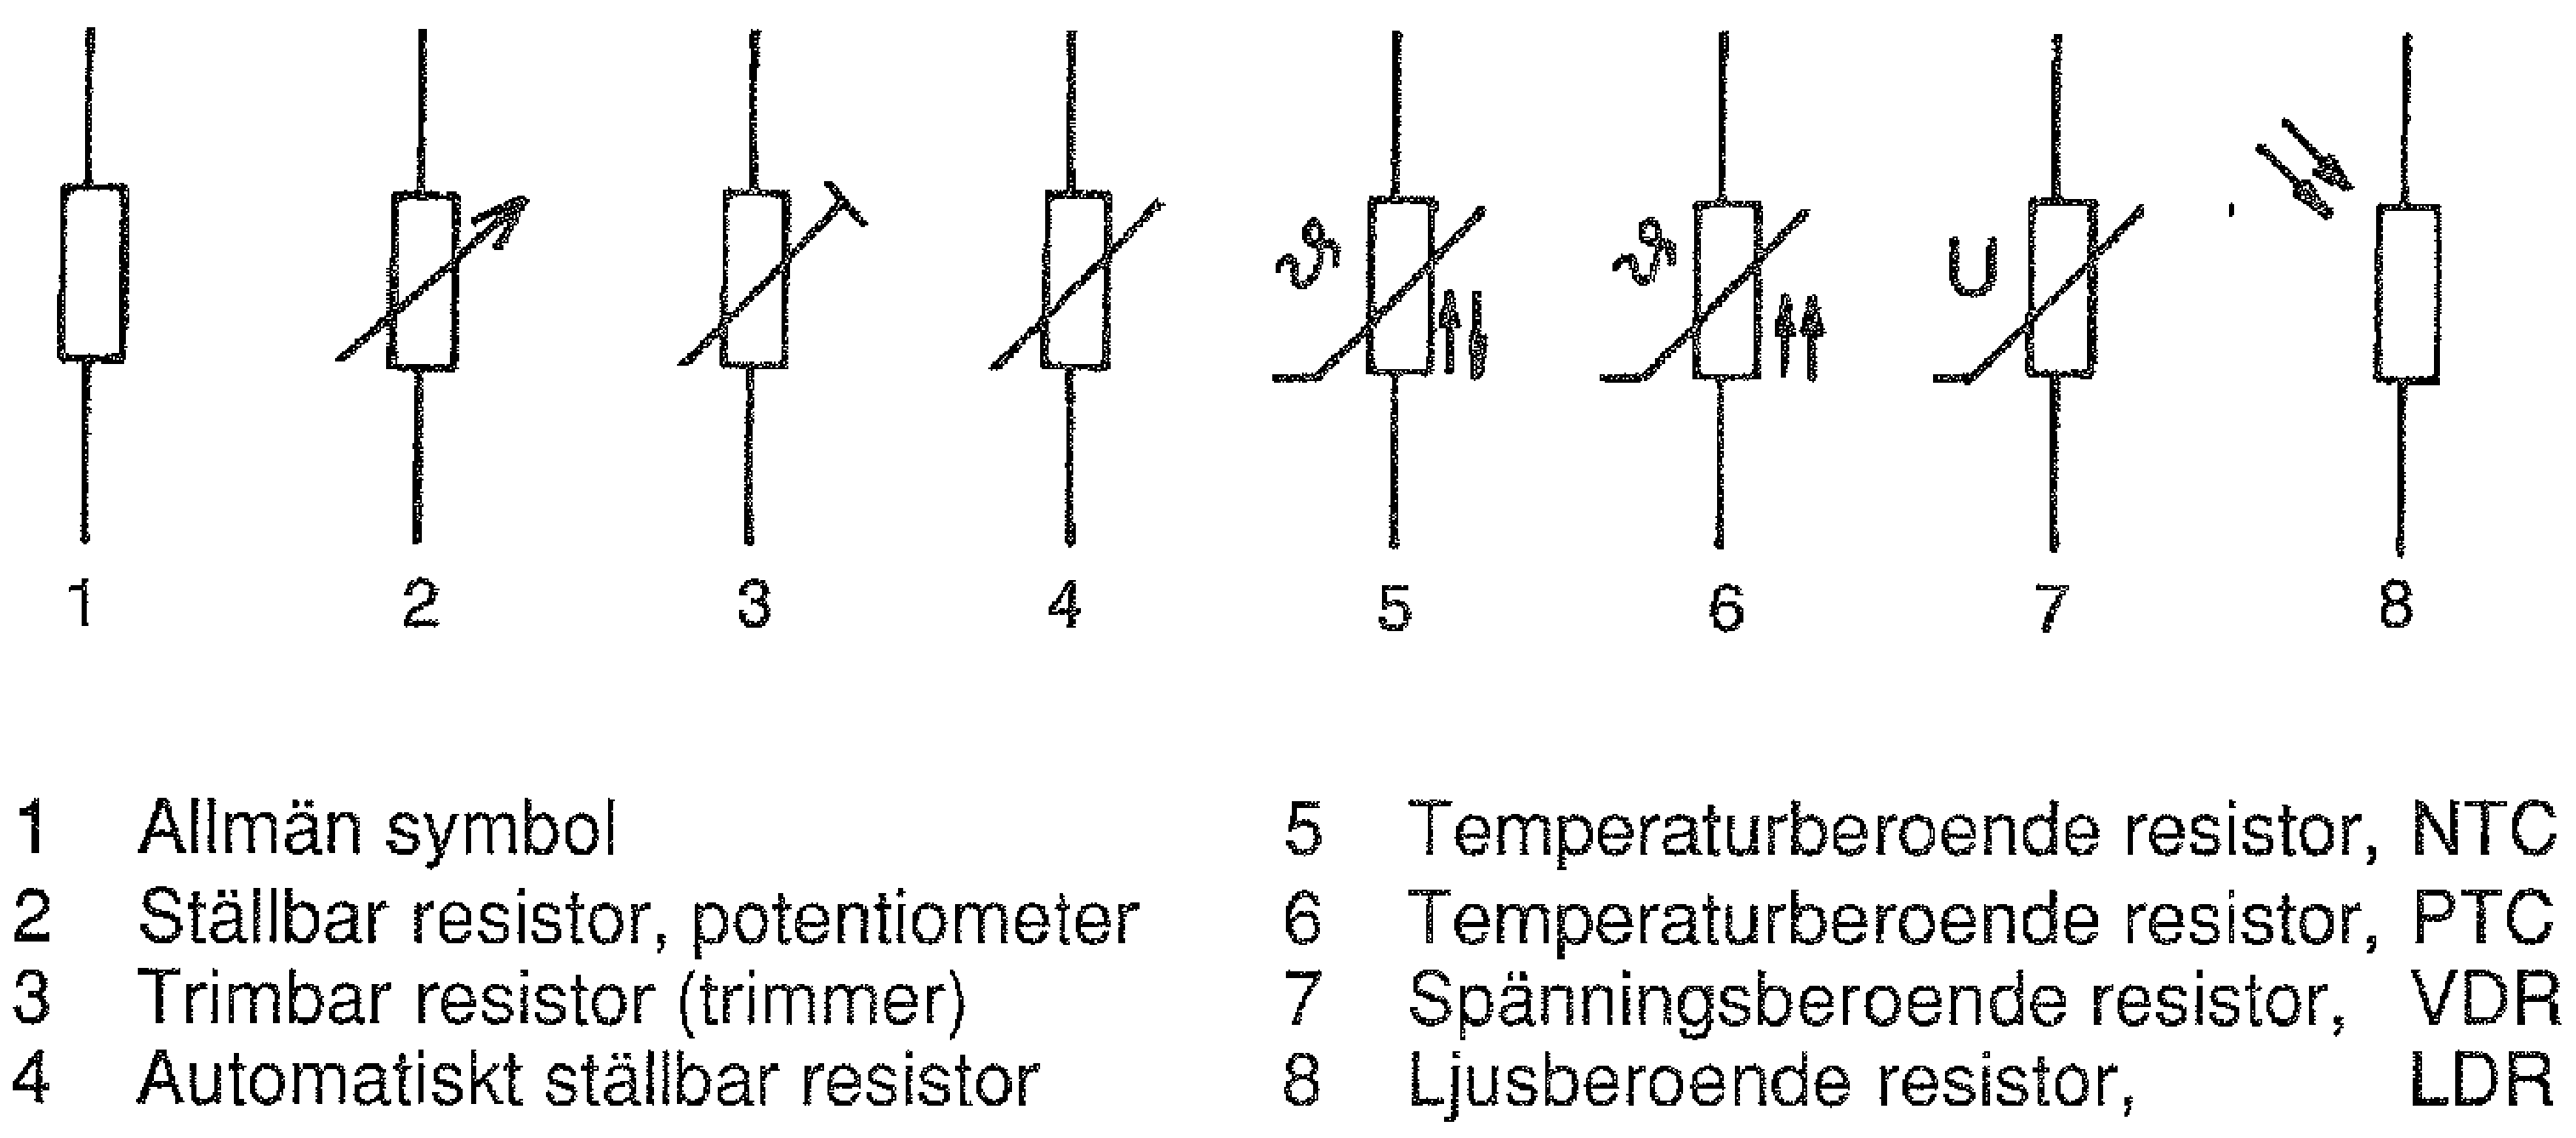
\includegraphics[width=\textwidth]{images/cropped_pdfs/bild_2_2-01.pdf}
\caption{Schemasymboler för resistorer}
\label{fig:BildII2-1}
\end{figure}

Bild \ref{fig:BildII2-1}

\subsection{Variabla resistorer}
\index{variabla resistorer}
\index{resistor!variabel}

En resistor kan även utföras med variabelt resistansvärde. Då används endast
den andel av det resistiva materialet, som finns mellan en resistors ena ände
och ett uttag någonstans mellan ändarna. En sådan anordning kallas för reostat.
Om en variabel resistor används som spänningsdelare, så kallas den för
potentiometer.

I en potentiometer används dels hela resistansen mellan ändpunkterna och dels
andelen mellan uttaget och någon av ändpunkterna. Uttagets mekaniska utförande
beror oftast av hur bekvämt inställningen ska kunna ske. En potentiometer,
där det resistiva materialet är lagt på en cirkulär bana och uttaget är fäst
vid en axel i banans centrum, medger enkel inställning med mejsel, ratt etc.
Ett enklare slags uttag är en släpkontakt eller ett spännband som kan flyttas
utmed en stavformad resistor.

\subsubsection{Resistiva material i variabla resistorer}

Banan i en variabel resistor består i princip av liknande resistiva material
som i en fast resistor. Billigast och enklast är en bana av kol, som är tryck
på ett enkelt underlag. Nackdelar är låg effekttålighet, dålig upplösning och
linjäritet, högt brus och kort livslängd. Fördelen är lågt pris.
Bättre än en kolbana är en bana av kolkomposit, d.v.s. kolpulver med bindemedel,
som är tryckt på ett underlag. Nackdel är högre pris och låg effekttålighet,
medan fördelarna är god upplösning, lågt brus och lång livslängd.
Vill man ha god effekttålighet och temperaturstabilitet, utöver kolkompositens
egenskaper, så erbjuder en bana av cermet sådana fördelar. En cermetbana består
av en blandning av metaller och keramik, som trycks på ett underlag.
Trådlindad bana har främst god tålighet mot hög effekt. Tålighet vid hög ström
genom uttaget är en annan fördel.

\subsubsection{Linjära och olinjära potentiometrar}

En potentiometer har en kurvform, varvid avses resistansändringen som funktion
av uttagets rörelseväg utmed resistansbanan. Kurvformen kan utföras linjär,
logaritmisk etc. Olinjära kurvor består då oftast av en följd av linjära
segment, som tillsammans någorlunda motsvarar den önskade olinjära formen. Ett
exempel på det är när en kurvform anges som linjär/logaritmisk.

\subsection{Effektutveckling i resistorer}
\textbf{HAREC a.\ref{HAREC.a.2.1.4}\label{myHAREC.a.2.1.4}}
\index{effektutveckling i resistorer}
\index{resistor!effektutveckling}

I resistorer utvecklas värme av den ström som flyter igenom. Värmeutvecklingen
sker enligt Joules lag, som återges i kapitel \ref{ellära}. Hur mycket effekt i form av
värme som strålas ut från resistorn beror på storleken på dess yta och
egentemperatur samt på omgivningens temperatur. Det finns en övre gräns för hur
stor värme det ingående materialet tål innan det förstörs och eventuellt fattar
eld. En resistors effekttålighet framgår i vissa fall av påstämplade värden.
I övriga fall är man hänvisad till kataloguppgifter eller en bedömning, som ev.
kan grundas på höljets utseende och dimensioner.

\subsection{Standardiserade komponentvärden}
\index{resistor!standardiserade värden}

Resistorer tillverkas vanligen med standardiserade värden ur någon talserie.

\subsection{Märkning av resistorer}

Resistorer märks med hjälp av siffror och bokstäver eller med en färgkod så att
resistorns huvuddata kan avläsas.
(Se f.ö. leverantörskataloger för information om komponentdata, märkning o.s.v.)

\section{Kondensatorn}
\textbf{HAREC a.\ref{HAREC.a.2.2}\label{myHAREC.a.2.2}}
\index{kondensator}

\subsection{Allmänt}

Så snart det finns en elektrisk potentialskillnad --- en spänning --- mellan två
kroppar, så uppstår ett elektriskt kraftfält mellan dem. Ett sådant fält är
lagrad elektrisk energi. Kropparna måste då isoleras från varandra.

Elektrisk energi lagras mellan olika delar av en strömkrets, även om de inte är
direkt avsedda för det. Särskilt vid mycket höga frekvenser har detta stor
betydelse för utformningen av en strömkrets. Vid låga frekvenser och likström
däremot, har kretsens utformning mindre inverkan. Då behövs i stället särskilda
anordningar för ta upp eller avge energi på önskade ställen i strömkretsen.

En sådan anordning kallas kondensator. Den består i princip av två band eller
plattor med anslutningsledningar samt ett isolerande skikt --- dielektrikum ---
däremellan. Kapacitansen är näst efter resistansen den vanligaste egenskapen i
en strömkrets.

\subsection{Kapacitans}
\textbf{HAREC a.\ref{HAREC.a.2.2.1}\label{myHAREC.a.2.2.1}}
\index{kapacitans}
\index{dielektricitet}
\index{symbol!\(C\) kapacitans}
\index{symbol!\(\epsilon_0\) dielektricitetskonstanten}
\index{symbol!\(\epsilon_r\) relativa dielektricitetskonstanten}

Förmågan att lagra elektrisk energi (elektrisk laddning) kallas
\emph{kapacitans} (eng. \emph{capacitance}).
Ordet kommer från latinets capax, som betyder rymlig, duglig.

Kapacitansen betecknas i formler med bokstaven C.

En kondensators kapacitans bestäms av ytan på kondensatorns plattor, avståndet
mellan dessa ytor, den absoluta dielektricitetskonstanten \(\epsilon_0\) och den
relativa dielektricitetskonstanten \(\epsilon_r\) som är den faktor kapacitansen
ökar med när dielektrikum är annat än vakuum.

Det isolerande materialet mellan plattorna kallas för \emph{dielektrum}
(eng. \emph{dielectrum}), och egenskaperna hos materialet påverkar kondensatorns
kapacitans.
Den egenskapen som materialet har kallas för \emph{dielektricitet}
(eng. \emph{dielectric property}) och uttrycks så som dess
\emph{dielektricitetskonstant} (eng. \emph{dielectric constant}).

Eftersom dielektriciteten ökar relativt den hos vakuum så använder man
dielektricitetskonstanten för vakuum \(\epsilon_0\) som en skalfaktor för att
omvandla den relativa dielektricitetskonstanten \(\epsilon_r\) till den
absoluta dielektricitetskonstanten \(\epsilon\).
\[
  \epsilon = \epsilon_0\epsilon_r
\]

Den relativa dielektriska konstanten går att hitta i tabeller och varierar
med material. Dielektricitetskonstanten för vakuum är definierad som
\[
  \epsilon_0 = \dfrac{1}{c_0^2\mu_0} \approx 8,854187 \cdot 10^{-12}
\]

\subsection{Kapacitans, dimension och dielektrikum}
\textbf{HAREC a.\ref{HAREC.a.2.2.3}\label{myHAREC.a.2.2.3}}
\index{dielektrum}
\index{kapacitans!dimension}
\index{kapacitans!dielektrum}

Kapacitansen är proportionell med den yta, som kondensatorplattorna skuggar
varandra, och är omvänt proportionell med plattavståndet.

Följande formler gäller för kapacitansen i en enkel kondensator med två
plattor. När en kondensator är uppbyggd av n stycken plattor, ökar kapacitansen
med faktorn (n-1).

Med vakuum som dielektrikum gäller sambandet 1 nedan och för ett godtyckligt
dielektrikum gäller sambandet 2.

\begin{enumerate}
  \item \(C = \varepsilon _0 \dfrac{A}{d}\)
  \item \(C = \varepsilon _0 \cdot \varepsilon _r \frac{A}{d}\)
\end{enumerate}

\(C\) är kapacitansen i farad [F], \(A\) är arean i kvadratmeter [m$^2$], $d$ är
avståndet i meter, $\varepsilon$ är dielektricitetskonstanten i farad per meter
[F/m].

\subsection{Enheten farad}
\textbf{HAREC a.\ref{HAREC.a.2.2.2}\label{myHAREC.a.2.2.2}}
\index{farad (F)}
\index{enheter!farad (F)}

Kapacitans är elektricitetsmängden per volt där måttenheten är \emph{farad} \unit{[F]}.
Eftersom denna enhet är mycket stor, används inom elektroniken oftast bråkdelar
av den.

\begin{table}[h]
\begin{tabular}{llcr}
 \SI{1}{mikrofarad} & \SI{1}{\micro\farad} &=& \num{1d-6} F \\
 \SI{1}{nanofarad}  & \SI{1}{\nano\farad}  &=& \num{1d-9} F \\
 \SI{1}{pikofarad}  & \SI{1}{\pico\farad}  &=& \num{1d-12} F
\end{tabular}
\caption{Kapacitansers förhållande till varandra}
\end{table}

\subsection{Kondensatorn i likströmskretsen}
\index{laddningsmängd}
\index{symbol!\(Q\) laddning}

En kondensator i en likströmskrets har alltid samma polaritet.
Därvid förhåller sig kondensatorns polspänning \(U\) till dess
\emph{laddningsmängd} \(Q\) och kapacitans \(C\) enligt sambandet
\[ U = C \cdot Q \]
\[ 	U \unit{[V]} \qquad C \unit{[F]} \qquad Q \unit{[As]} \]

Laddningsmängd har enheten ampere gånger sekund och är alltså ett mått på hur
många laddningar som har samlats.

En ström flyter till kondensatorn och laddar upp den, när den anslutna
spänningskällan har högre spänning än kondensatorn. Ju högre spänningen är,
desto större är laddningen. Ju kortare uppladdningstiden är, desto högre effekt
utvecklas under den tiden.

När en uppladdad kondensator ansluts till en krets med lägre spänning, så
urladdas kondensatorn till kretsen. Ju kortare urladdningstiden är, desto högre
effekt utvecklas under den tiden.

Laddningen i en kondensator kan innebära hög polspänning. Om kondensatorns
kapacitet är stor, kan laddningsmängden bli betydande. Varning för elektriska
stötar och brännskador!

\subsection{Kondensatorn i växelströmskretsen}

I en likströmskrets förhåller sig kondensatorns polspänning till
laddningsmängden. I en växelströmskrets växlar emellertid spänningen och
polariteten ständigt och därmed kondensatorns laddning och polaritet.

\marginnote{OBSERVERA: Vissa kondensatortyper kan inte användas i rena
  växelströmskretsar.}

\paragraph{Försök:}

En glödlampa och en kondensator kopplas i serie med varandra och ansluts till en
växelströmskrets. Med lämpligt valda värden på komponenterna kommer lampan att
lysa upp.

Detta visar att en kondensator inte hindrar elektronflödet i en växelström
krets. Man brukar säga att kondensatorn ''släpper igenom växelström'', men i
stället är det så att laddningar pendlar mellan kondensatorns plattor genom den
strömkrets som kondensatorn är ansluten till.

Använd för säkerhets skull låg spänning, t.ex. den från en
ringledningstransformator!

\subsection{Kapacitiv reaktans}
\textbf{HAREC a.\ref{HAREC.a.2.2.4}\label{myHAREC.a.2.2.4}}
\index{kapacitiv reaktans}
\index{kapacitans!reaktans}
\index{kondensator!reaktans}
\index{reaktans!kapacitiv}
\index{symbol!\(X_c\) kapacitiv reaktans}

Strömstyrkan i en växelströmskrets beror bl.a. på hur stor kondensatorns
kapacitans är, dvs. på dess \emph{kapacitiva reaktans} (eng.
\emph{capacitive reactance}) \(X_c\).

Ordet reaktans kommer från latinets \emph{re} (åter) \emph{agere} (verka).

Större kapacitans innebär större förmåga att ta upp elektrisk laddning och ger
därmed en lägre reaktans. Resultatet blir ett kraftigare elektronflöde.
En mindre kapacitans innebär ett svagare elektronflöde.

Sambandet tecknas:

\[
X_C = \frac{1}{2\pi fC} \qquad \mathrm{eller} \qquad X_C = \dfrac{1}{\omega C}
\]
Storheter och enheter hänger samman enligt följande:
\[
	X_C\ \unit{[\ohm]} \qquad 
	f\ \unit{[Hz]} \qquad 
	C\ \unit{[F]}
\]


\noindent\emph{Exempel 1:} Kapacitansen \SI{10}{\micro\farad} och frekvensen \SI{50}{Hz} --- vad blir den kapacitiva reaktansen?

\[ C = \SI{10}{\micro\farad} \qquad f = \SI{50}{\hertz} \qquad X_c = ? \]
\[
X_c = \frac{1}{2 \pi f C} = 
\frac{1}{2\pi 50 \cdot 10 \cdot 10^{-6}} = 
\SI{318,3}{\ohm}
\]

\noindent\emph{Exempel 2:} Givet en kapacitans på 10\,µF och frekvensen 5\,kHz vad blir den resulternde kapacitiva reaktansen?
\[ C = \SI{10}{\micro\farad} \qquad f = \SI{5}{kHz} \qquad X_c = ? \]
\[
X_c = \frac{1}{2\pi f C} = \frac{1}{2\pi 5 \cdot 10^3 \cdot 10 \cdot 10^{-6}}
= \SI{3,183}{\ohm}
\]


En kondensators reaktans är således omvänt proportionell med dess kapacitans
och frekvensen i kretsen.

\marginnote{Detta kan nyttjas genom att man kopplar samman reaktanser och
	 kapacitanser på olika sätt kan man skapa filter som släpper igenom enbart vissa frekvenser --- en vital del i varje radioutrustning!}
Jämför detta med en induktor där reaktansen är proportionell med frekvensen.

När en ström flyter genom en resistor, så uppstår det värmeförluster. När ström
flyter genom en ideal reaktans --- en ideal induktor eller kondensator --- uppstår
däremot inga värmeförluster.

\subsection{Fasförskjutning i en kondensator}
\textbf{HAREC a.\ref{HAREC.a.2.2.5}\label{myHAREC.a.2.2.5}}
\index{fasförskjutning!kondensator}
\index{kondensator!fasförskjutning}

Med fasförskjutning menas här den tidsmässiga förskjutningen mellan ström- och
spänningsförloppen. I en kondensator når nämligen strömmen inte sitt toppvärde
samtidigt som spänningen.
I en ideal kondensator är spänningen fasförskjuten 90\degree~efter strömmen.

\subsection{Förlustvinkel}
\index{förlustvinkel}

I praktiken är fasförskjutningen i en kondensator något mindre än 90\degree\ på
grund av att laddning läcker igenom dielektrikum. Man talar om en förlustvinkel.
Läckningen kan ses som en resistor som är kopplad parallellt över kondensatorn.

\subsection{Läckström m.m.}
\index{läckström}
\index{kondensator!läckström}

Med sitt extremt tunna dielektrikum har elektolytkondensatorn en mycket högre
kapacitet än andra former, men har också några nackdelar, bl.a. att den normalt
endast kan användas med likspänning, den har hög förlustfaktor på grund av läckström,
och det utvecklas värme av läckströmmen, vilket skapar övertryck på grund av
gasbildning.

\subsection{Utförandeformer}

Kondensatorer kan utföras med fast kapacitansvärde.
Dielektrikum består då av ett skikt av glimmer, impregnerat papper osv.

Kondensatorer kan även utföras med variabelt kapacitansvärde.
Dielektrikum består då oftast av luft, men kan även vara ett fast material.

\subsubsection{Fasta kondensatorer}

\begin{figure}[ht]
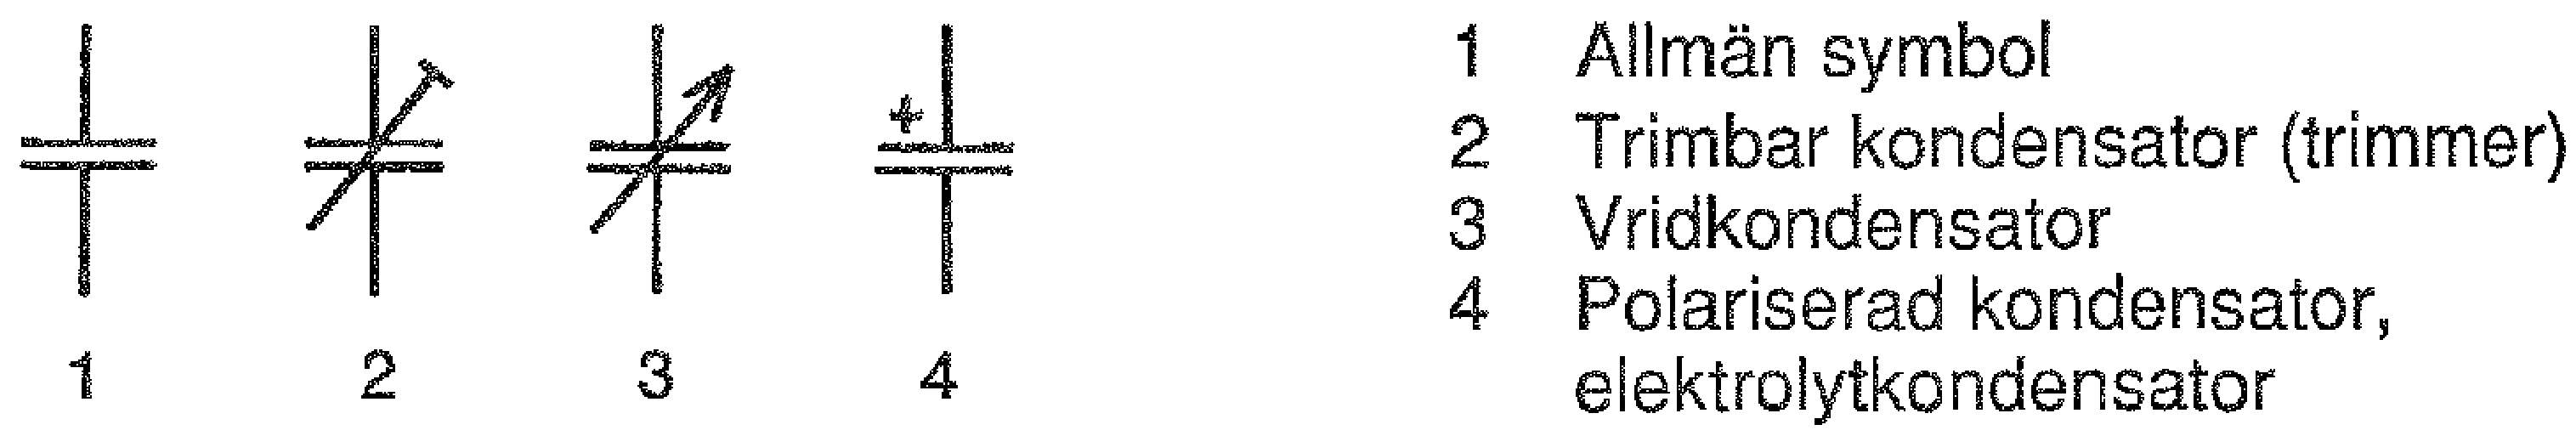
\includegraphics[width=\textwidth]{images/cropped_pdfs/bild_2_2-02.pdf}
\caption{Schemasymboler för kondensatorer}
\label{fig:BildII2-2}
\end{figure}

Bild \ref{fig:BildII2-2}

Kondensatorer har oftast namn efter utförande och materialet i dielektrikum.

\emph{Pappers- och plastkondensatorer}

''Plattorna'' i dessa typer består av aluminiumremsor med anslutningstrådar.
Däremellan finns en pappers- respektive plastremsa som dielektrikum. För att
spara plats, så rullas det hela ihop och skyddas med en plastingjutning.

\emph{Keramiska kondensatorer}

I keramiska kondensatorer består dielektrikum av något keramiskt material.
På ömse sidor om detta sätts en metallbeläggning med anslutningstrådar.

\emph{Glimmerkondensatorer}

I denna kondensatortyp består dielektrikum av tunna glimmerskivor.

\emph{Elektrolytkondensatorer}

Elektrolytkondensatorer har elektroder av aluminium eller tantal, där pluspolen
(anoden) ges ett mycket tunt oxidskikt. Detta är inte ledande och fungerar som
dielektrikum. Mellan oxidskiktet och minuspolen (katoden) läggs en elektrolyt
med låg resistivitet.

Elekrolytkondensatorer har särskilt högt kapacitansvärde. Till skillnad från
andra kondensatortyper, så är elektolytkondensatorer polariserade. Utom i ett
specialfall innebär det, att polariteten på den pålagda spänningen inte får
kastas om. Flera olika slags elektrolytkondensatorer finns, så som våta
och torra aluminiumelektrolytkondensatorer, tantalelektrolytkondensatorer m.fl.

\subsubsection{Variabla kondensatorer}
Variabla kondensatorer har oftast sitt namn efter utförandeformen, så som
vridkondensator och trimbar kondensator (trimmer).

\subsection{Temperaturkoefficient}
På liknande sätt som med resistorer, så påverkas kapaciteten i kondensatorer av
temperaturen. Att sambandet mellan kapacitet och temperatur är viktigt, förstås
av att temperaturkoefficienten i den frekvensbestämmande kapacitansen i en
oscillatorkrets är en av faktorerna för stabil frekvens.

Temperaturkoefficienten \(\alpha _c\) anger kapacitetsändringen per grad temperaturändring.
Kapacitetsändringen blir då

\[  \Delta C = \pm \alpha _c \cdot C_k \cdot \Delta\vartheta  \]

varvid \(C_k\) är kapacitetsvärdet vid den lägre temperaturen (oftast 20~\degree C) och
\(\Delta\vartheta\) är temperaturändringen i kelvin.
Kelvin [K] är den normerade måttenheten för absolut temperatur.
En ändring med 1\,K motsvarar en ändring med 1\degree\,C.

Är \(\alpha _c\) positivt betyder det att kapaciteten ökar med ökande
temperatur. Är \(\alpha _c\) negativt betyder det att kapaciteten minskar med ökande
temperatur.

En kondensator som är märkt med N 100 betyder:
\[ \alpha _c = -100 \cdot 10^{-6} 1/\unit{K}  \]

%\subsection{Standardiserade komponentvärden}
\index{kondensator!standardiserade värden}

Kondensatorer tillverkas vanligen med standardiserade värden från en talserie.

\subsection{Märkning av kondensatorer}

Kondensatorer märks med hjälp av siffror och bokstäver eller med en färgkod så att
kondensatorns huvuddata kan avläsas.

\section{Induktorn}
\textbf{HAREC a.\ref{HAREC.a.2.3}\label{myHAREC.a.2.3}}
\index{induktor}

\subsection{Allmänt}

När elektrisk ström flyter genom en ledare, så alstras ett magnetfält omkring
den. Så snart strömmens styrka eller riktning ändras, uppstår en motsvarande
s.k. elektromotorisk kraft (EMK), som motverkar ändringen. Kraften finns i
magnetfältet, som är lagrad magnetisk energi.


\subsection{Självinduktion -- induktans}
\textbf{HAREC a.\ref{HAREC.a.2.3.1}\label{myHAREC.a.2.3.1}}
\index{induktans}
\index{självinduktion}
\index{EMK}
\index{induktor}

Magnetfältets förmåga att alstra en motverkande EMK kallas
\emph{självinduktion} (eng. \emph{self inductance}) eller
\emph{induktans} (eng. \emph{inductance}).
Ordet induktans kommer från latinets inducere, som betyder införa.

När en ledare, som ingår i en sluten krets, rör sig i ett magnetfält, så kommer
en ström att flyta genom ledaren på grund av den EMK (spänning) som alstras.
Varje ändring av strömmen motverkas av det magnetfält som strömmen själv
alstrar.

När det uppstår självinduktion i en ledare, så kallas ledaren \emph{induktor}
(eng. \emph{inductor}).
Självinduktionen är jämnt utbredd över ledarens hela längd. När ett större
induktansvärde behövs på något särskilt ställe i strömkretsen, så kan ledarens
längd ökas just där och lindas upp till en spole med lämplig form.
Hela spolen kallas då för induktor.

Det att ett motverkande magnetiskt fält alstras omkring en ledare när strömmen i
den ändras, påverkar kretsens egenskaper och därmed utformning på olika sätt.
Vid snabba strömändringar, t.ex. vid hög frekvens, är motverkan större än vid
långsamma ändringar.
Vid konstant likström uppstår däremot ingen motverkan -- självinduktion.

Induktansen är efter resistansen och kapacitansen den vanligaste egenskapen i
en strömkrets.

\subsection{Försök med induktion}

\emph{Försök 1}

\begin{figure}
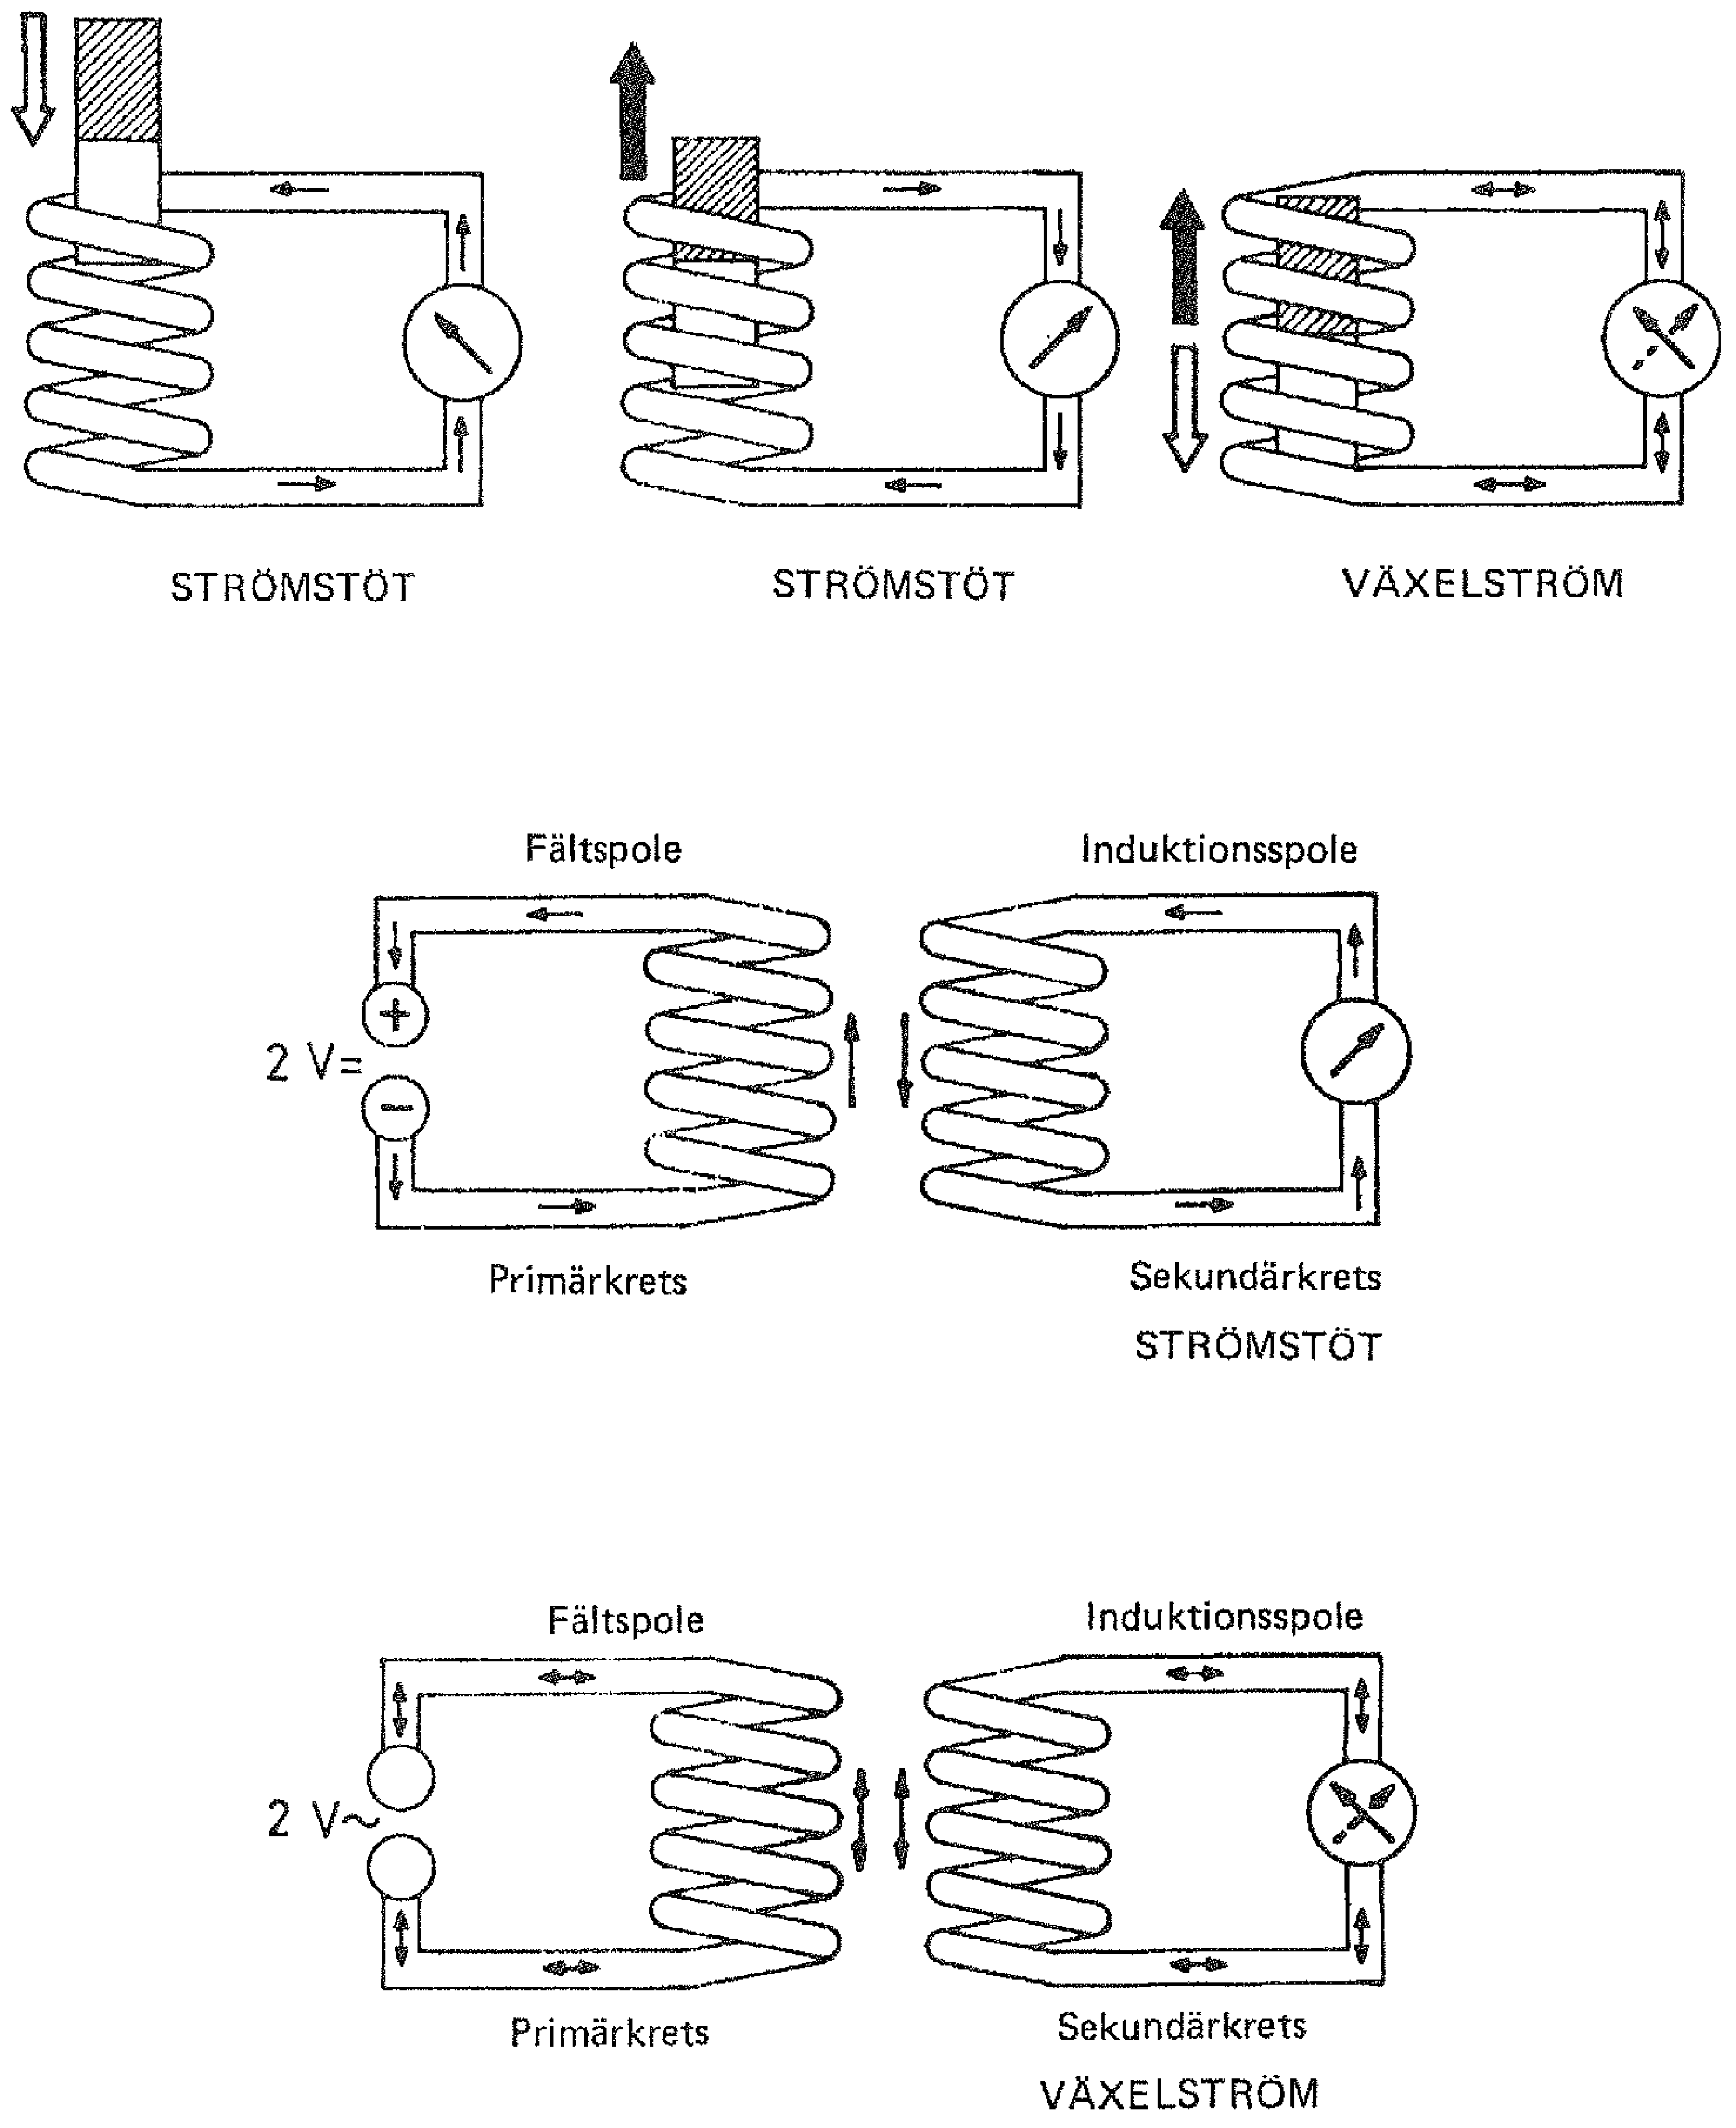
\includegraphics[width=\textwidth]{images/cropped_pdfs/bild_2_2-03.pdf}
\caption{Försök med induktion}
\label{fig:BildII2-3}
\end{figure}

I bild \ref{fig:BildII2-3} överst är ett känsligt vridspoleinstrument kopplas
till en induktor.
Instrumentet bör ha noll på skalans mitt, så att strömriktningen syns.
En permanentmagnet används för att visa att självinduktion uppstår när
magneten förs fram och tillbaka genom induktorn.

Instrumentet ger utslag när magneten är i rörelse. Utslaget blir större vid
snabbare hastighetsändring. Utslagsriktningen växlar, när magneten förs in i
respektive dras ut ur induktorn -- det uppstår en växelström.

En växelspänning uppstår över induktorn, även när den ingår i en strömkrets som
sluts och bryts -- alltså utan en magnet som rör sig.

\emph{Försök 2}

I bild \ref{fig:BildII2-3} mitten har permanentmagneten byts nu mot ännu en
induktor.
Utöver den första induktorn, som vi nu kallar sekundärlindning, kallar vi den
nya induktorn för primärlindning.

När vi släpper ström genom primärlindningen så alstrar den ett magnetfält.
Först är strömmen noll för att sedan ändras till ett högt värde och därefter
återgå till noll. Det blir en strömstöt.

Varje ändring alstrar en mot-emk, som bygger upp ett magnetfält, först i en
riktning och sedan i den andra. I båda fallen passerar fältet genom båda
lindningarna. Fältet från primärlindningen inducerar en spänningsstöt i
sekundärlindningen. Stöten har en riktning, när primärlindningens strömkrets
sluts och motsatt riktning när den bryts, d.v.s. det blir en växelspänning.
När sekundärlindningen ingår i en sluten krets, uppstår en växelström genom
sekundärlindningen.

\emph{Försök 3}

I bild \ref{fig:BildII2-3} nederst ställer vi oss frågan vad som händer när
primärlindningen i försök 2 ansluts till en växelspänning, t.ex.
med nätfrekvensen 50~Hz? Använd för säkerhets skull en skyddstransformator
mellan nätet och lindningen!

I sekundärlindningen uppstår då spänningsstötar, vars polaritet i detta fall
växlar 100 gånger per sekund. Det uppstår alltså en växelspänning över
sekundärlindningen och om denna ingår i en sluten strömkrets uppstår det en
motsvarande växelström.


\begin{figure}
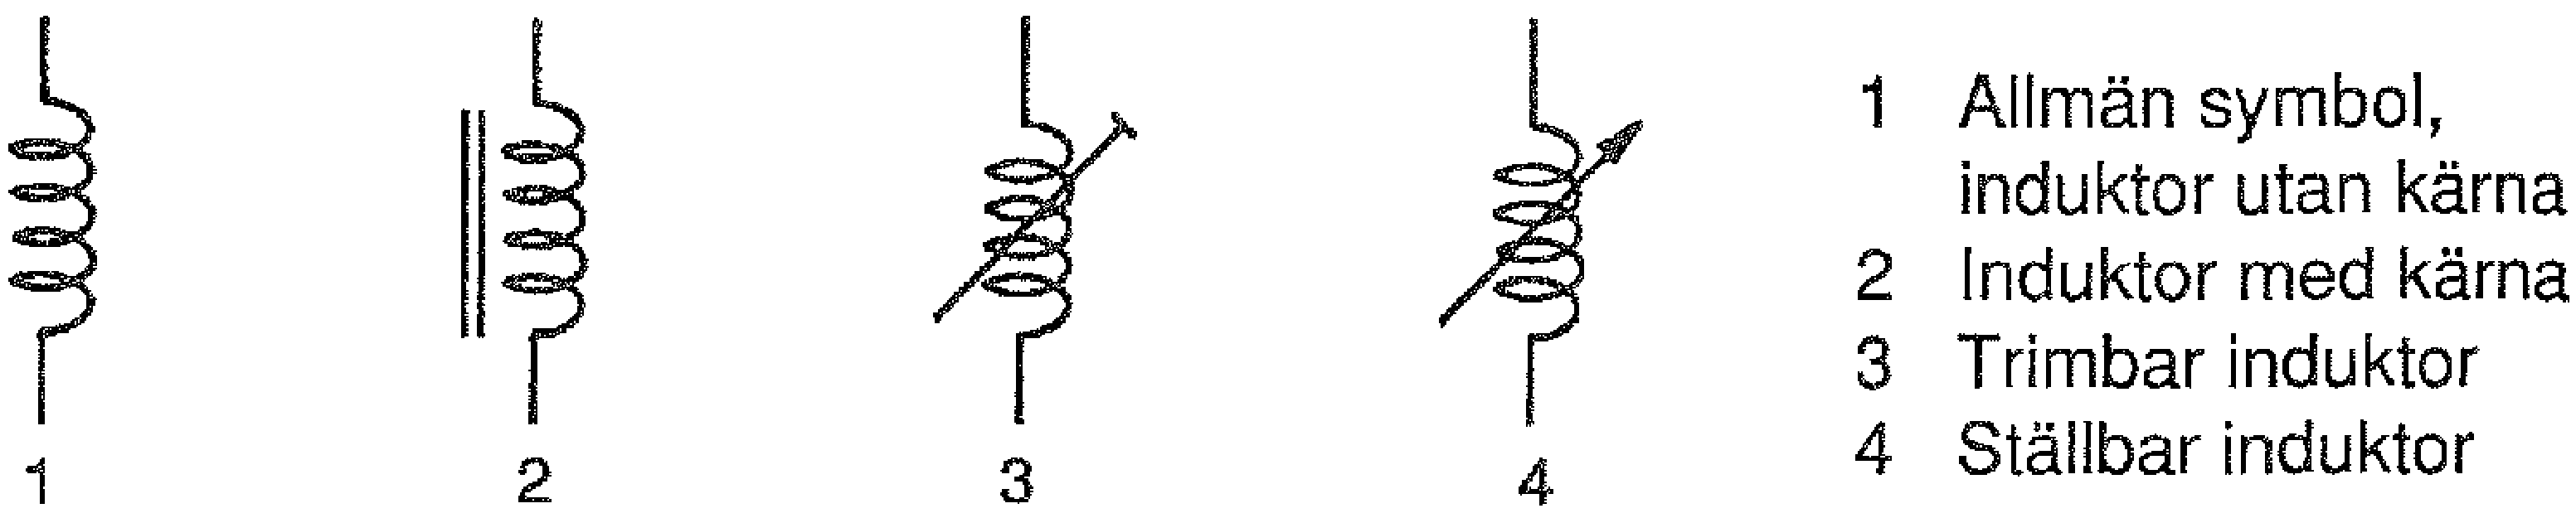
\includegraphics[width=\textwidth]{images/cropped_pdfs/bild_2_2-04.pdf}
\caption{Schemasymboler för induktorer}
\label{fig:BildII2-4}
\end{figure}

\subsection{Olika utföranden}

Bild \ref{fig:BildII2-4} visar schemasymboler för ett antal vanliga induktorer.
Utöver dessa finns Elektromagneter, drosslar, induktorer för svängningskretsar,
ramantenner o.s.v.

\subsection{Enheten henry (H)}
\textbf{HAREC a.\ref{HAREC.a.2.3.2}\label{myHAREC.a.2.3.2}}
\index{henry (H)}
\index{enheter!henry (H)}
\index{symbol!\(L\) induktans}

Måttenheten för självinduktion är \emph{henry (H)}.
1~henry (1~H) är självinduktionen i en induktor, som alstrar en motspänning av
1~volt vid en strömändring av 1~ampere under 1~sekund.

I formler betecknas induktans med symbolen L.

Sambandet är

\(volt = henry \cdot ampere/sekund\)

1~H är en stor måttenhet. För elektroniktillämpningar används därför ett mer
hanterligt format.

Exempel:

\begin{tabular}{ll}
\(1\ H \) & \(= 1000\ mH\) \\
\(1\ mH\) & \(= 1 \cdot 10^{-3}\ H\) \\
\(1\ mH\) & \(= 1000\ \mu H\) \\
\(1\ \mu H\) & \(= 1 \cdot 10^{-3}\ mH = 1 \cdot 10^{-6}\ H \)
\end{tabular}

\subsection{Hur induktansen påverkas}
\textbf{HAREC a.\ref{HAREC.a.2.3.3}\label{myHAREC.a.2.3.3}}
\index{permabilitet}
\index{relativa permabiliteten}
\index{symbol!\(\mu_0\) permabilitetskonstanten}
\index{symbol!\(\mu_r\) relativa permabiliten}

Induktansen beror på induktorns mekaniska dimensioner, antalet lindningsvarv och
materialet i kärnan.

Induktansen i en cylindrisk induktor är proportionell mot tvärsnittsytan, omvänt
proportionell mot längden och proportionell mot kvadraten på lindningsvarvtalet.

Induktansen ökar, om induktorn förses med en kärna av järn och minskar med en
kärna av omagnetisk, ledande metall, t.ex. koppar, mässing eller aluminium.

Precis som för kondensatorn så har materialet i en induktorns kärna betydelse,
då dess \emph{permabilitet} kan anta olika värden. Den absoluta permabiliteten
\(\mu\) brukar delas upp i permabiliteten för vakuum \(\mu_0\) och den
\emph{relativa permabiliteten} \(\mu_r\) som gives av

\(\mu = \mu_0\mu_r\)

Den relativa permabiliteten går att hitta i tabeller och varierar med material.
Dielektricitetskonstanten för vakuum är definierad som

\(\mu_0 = 4\pi 10^{-7} \approx 1,256637 \cdot 10^{-6}\)

\subsection{Induktiv reaktans}
\textbf{HAREC a.\ref{HAREC.a.2.3.4}\label{myHAREC.a.2.3.4}}
\index{induktiv reaktans}
\index{reaktans!induktiv}
\index{symbol!\(X_L\) induktiv reaktans}

Till skillnad från när en resistor ansluts till en spänning, så blir
strömökningen i en induktor fördröjd. Orsaken är att en induktor inte bara har
en resistans, vilken ju inte påverkas av strömvariationer, utan har även en
\emph{induktiv reaktans} (eng. \emph{inductive reactance}) \(X_L\).
Ordet reaktans kommer från latinets re (åter) agere (verka).

\emph{Reaktans} -- växelströmsmotstånd eller skenbart motstånd -- uppträder så
länge som strömmen genom induktorn ändras. En induktor gör således också
motstånd mot varje strömändring och detta motstånd ökar med ökande
ändringshastighet.

En fullbordad pendling i en växelström kan ses som ett varv i en cirkel --
360\degree -- och en fullbordad pendling kallas en period.

En period motsvarar omkretsen i en cirkel med radien r, där omkretsen är
\(2 \cdot \pi  \cdot r\). När strömmen växlar 1 gång/sekund har
pendlingen en frekvens [f] av 1~Hertz [Hz]. Vid 50 växlingar/sekund har
pendlingen en frekvens av 50~Hz o.s.v.

\emph{Induktiva reaktansen \(X_L\)} -- växelströmsmotståndet i en induktor -- är
en funktion av strömmens s.k. vinkelhastighet \(\omega = 2 \cdot \pi  \cdot f\)
och av storheten av induktansen L.

Den induktiva reaktansen är proportionell mot strömmens frekvens och mot
induktorns induktansvärde. Inga förluster uppstår i en ideal induktor, d.v.s. en
som teoretiskt saknar resistans.

Sambandet är
\(X_L = 2\pi fL = \omega L\)

\begin{tabular}{llll}
 \(X_L [\Omega]\) & \(f [Hz]\) & \(L [H]\)
 \end{tabular}

\textbf{Exempel:}

1. \(L = 1\ H\) \(f = 50\ Hz\) \(X_L = ?\)

\(X_L = 2\pi fL = 2\pi  \cdot 50 \cdot 1 = 314\ \Omega\)

2. \(L = 1\ H\) \(f = 5\ kHz\) \(X_L = ?\)

\(X_L = 2\pi fL = 2\pi  \cdot 5 \cdot 10^3 \cdot 1 = 31\, 400\ \Omega\)

\subsection{Fasförskjutning mellan spänning och ström i en induktor}
\textbf{HAREC a.\ref{HAREC.a.2.3.5}\label{myHAREC.a.2.3.5}}
\index{induktor!fasförskjutning}

Med fasförskjutning menas den tidsmässiga förskjutningen mellan ström- och
spänningsförlopp. Strömmen genom en induktor, når inte sitt toppvärde samtidigt
som spänningen över den. Orsaken är växlingarna mellan elektrisk och magnetisk
energi i induktorn.
Detta illustreras i bild \ref{fig:BildII3-11}.

I en ideal induktor är spänningen fasförskjuten 90\degree~före strömmen.
I praktiken är dock förskjutningen något mindre än 90\degree~på grund av
resistansen i induktorn.

\subsection{Q-faktor -- godhetstal}
\textbf{HAREC a.\ref{HAREC.a.2.3.6}\label{myHAREC.a.2.3.6}}
\index{Q-faktor!induktor}

\emph{Q-faktorn} kan avse två olika saker, som inte ska förväxlas.
Det är Q-faktorn för en komponent respektive den för en hel strömkrets.

Q-faktorn för en induktor är kvoten av dess reaktans och serieresistans.

\(Q_\text{komponent} = \dfrac{X_\text{komponent}}{R_\text{komponent}}\)

Q-faktorn för en hel svängningskrets beror däremot på bredden på det
frekvensband som en viss komponentkombination ger.
Q-faktorn för en resonant svängningskrets är därför ett mått på dess
selektivitet (se kapitel \ref{Q-faktor}).

Medan Q-faktorn för en ingående komponent påverkar Q-faktorn för en hel krets,
så gäller inte det omvända.

\subsection{Yteffekt -- skin-effect}
\index{yteffekt}
\index{skin-effect}

I en ledare av homogent material fördelar sig en likström lika över hela
tvärsnittet. Strömtätheten för en växelström däremot, minskar i ledarens mitt
och ökar i stället vid ytan.
Ju högre frekvensen är, desto större är strömtätheten vid ytan.
Fenomenet kallas \emph{yteffekt} (eng. \emph{skin effect}) och uppträder i alla
ledare.

Det djup i ledarmaterialet där laddningstätheten sjunkit till 37~\% av
värdet vid ytan kallas \emph{skin depth}. För koppar är detta djup ca 70~mm vid
100~Hz. Vid 1~MHz har djupet minskat till 0,07~mm och vid 100~MHz till
0,0067~mm. På grund av yteffekten är alltså materialet i mitten av homogena
ledare elektriskt mindre verksamt vid höga frekvenser. Resistansen blir alltså
större för växelström än för likström, om ledaren är samma.

Utöver frekvensen påverkas yteffekten av ledarmaterialets elektriska och
magnetiska ledningsförmåga. För att få låg resistans i ledare för högfrekvent
ström är det viktigt att omkretsen är stor och att materialskiktet vid ytan har
hög ledningsförmåga. Det är därför som induktorerna i sändarslutsteg ofta är
försilvrade och består av rör med stor diameter eller av breda band.

\subsection{Temperaturkoefficient}

Liksom med resistorer, så påverkas induktansen av temperaturen. Att sambandet
mellan induktans och temperatur är viktigt, förstås av att
temperaturkoefficienten i den frekvensbestämmande induktorn i en oscillatorkrets
påverkar frekvensstabiliteten.

Eftersom metallen koppar utvidgar sig vid temperaturökning och induktorns
tvärsnittsyta då blir större, så är temperaturkoefficienten vanligen positiv.
Temperaturkoefficienten \(\alpha_L\) anger induktansändringen per grad
temperaturändring.

Induktansändringen blir då

\(\Delta L = \pm \alpha _L \cdot L_k \cdot \Delta\vartheta\)

varvid \(L_k\) är induktansvärdet vid den lägre temperaturen (oftast
20~\degree C) och \(\Delta\vartheta\) är temperaturändringen i kelvin.

Kelvin [K] är den normerade måttenheten för absolut temperatur.
En ändring med 1~K motsvarar en ändring med 1~\degree C.

Induktorer kan innehålla kärnor av någon metallegering, vars egenskaper också är
temperaturberoende.

I praktiken kan man knappast påverka temperaturkoefficienten i en induktor.
Eftersom en svängningskrets för det mesta även innehåller kondensatorer, så kan
man t.ex. kompensera en positiv temperaturkoefficient i induktorn med en negativ
i en kondensator.

\subsection{Förluster i kärnmaterial}

När ett magnetiskt växelfält passerar ett kärnmaterial så kommer atomerna (som
är permanentmagneter) att ständigt inta nya lägen i materialet i takt med
fältets frekvens. Då uppstår virvelströmmar, s.k. järnförluster, som dels
påverkar materialets ledningsförmåga och dels höjer temperaturen i kärnan och
därmed i hela induktorn.

\section{Transformatorn}
\textbf{HAREC a.\ref{HAREC.a.2.4}\label{myHAREC.a.2.4}}
\label{transformator}
\label{primärlindning}
\label{transformator!primärlindning}
\label{sekundärlindning}
\label{transformator!sekundärlindning}

\subsection{Allmänt}

En \emph{transformator} (eng. \emph{transformer}) består av en eller flera
lindningar eller spolar av elektriska ledare.
Lindningarna är magnetiskt kopplade till varandra.
Det innebär att de är anordnade så, att ett magnetfält, som alstrats i någon
av lindningarna, även passerar genom övriga lindningar.

När en växelspänning läggs över en lindning, kallas den \emph{primärlindning}
(eng. \emph{primary coil}).
I och omkring primärlindningen alstras då ett magnetiskt fält som växlar i takt
med spänningen. Primärfältet passerar även genom övriga lindningar --
\emph{sekundärlindningarna} (eng. \emph{secondary coil}) -- och alstrar där
spänningar och strömmar.

Den s.k. kopplingsfaktorn mellan lindningarna varierar för olika frekvenser,
sämre vid låga frekvenser (hundratals Hz) och bättre vid höga frekvenser
(tusentals Hz).
Speciellt vid låga frekvenser behövs en bättre koppling för att avsedd
effekt ska kunna överföras mellan lindningarna. Då kan ledningsförmågan i den
magnetiska flödesvägen ökas med hjälp av en järnkärna.

\begin{figure}[ht]
%  \begin{mdframed}
    \begin{center}
      \begin{circuitikz}
        \draw
        (1,1) node[transformer](T1) {}
        (T1.base) node{1}
        ;
        \draw[european]
        (4,1) node[transformer](T2) {}
        (T2.base) node{2}
        ;
        \draw
        (7,1) node[transformer core](T3) {}
        (T3.base) node{3}
        ;
      \end{circuitikz}
      \\
      \begin{tabular}{ll}
        1, 2 & Allmänna symboler \\
        3 & Transformator med kärna
      \end{tabular}
    \end{center}
    \caption{Schemasymboler för transformatorer}
%  \end{mdframed}
  \label{fig:BildII2-5}
\end{figure}

Bild \ref{fig:BildII2-5} illustrerar flera vanligt förekommande schemasymboler
för transformatorer med två lindningar.

\subsection{Utföranden}
\index{spänningstransformator}
\index{transformator!spännings-}
\index{strömtransformator}
\index{transformator!ström-}
\index{impedanstransformator}
\index{transformator!impedans-}

Transformatorn kan utföras för olika ändamål, t.ex. som
\emph{spänningstransformator} (eng. \emph{voltage transformer}),
\emph{strömtransformator} (eng. \emph{current transformer}) eller
\emph{impedanstransformator} (eng. \emph{impedance transformer}).

Utförandet påverkas även av överförd effekt och frekvens.

\subsection{Terminologi}
\index{varvtalsomsättning}
\index{transformator!varvtalsomsättning}
\index{impedansomsättning}
\index{transformator!impedansomsättning}

\begin{tabular}{ll}
primärkrets & sekundärkrets \\
primärlindning & sekundärlindning \\
primärspänning \(u_1\) &  sekundärspänning \(u_2\) \\
primärström \(i_1\) & sekundärström \(i_2\) \\
lindningsvarvtal n & primärt \(n_1\) sekundärt \(n_2\)
\end{tabular}

varvtalsomsättning = \(\dfrac{n_1}{n_2}\) eller \(\dfrac{n_2}{n_1}\)

impedansomsättning = \(\dfrac{Z_1}{Z_2}\) eller \(\dfrac{Z_2}{Z_1}\)

\subsection{Den ideala (förlustfria) transformatorn}
\textbf{HAREC a.\ref{HAREC.a.2.4.1}, a.\ref{HAREC.a.2.4.2.1},
a.\ref{HAREC.a.2.4.2.2}\label{myHAREC.a.2.4.1}
\label{myHAREC.a.2.4.2.1}\label{myHAREC.a.2.4.2.2}}
\index{varvtalsomsättning}
\index{transformator!varvtalsomsättning}
\index{impedansomsättning}
\index{transformator!impedansomsättning}

\begin{figure*}[ht]
\begin{center}
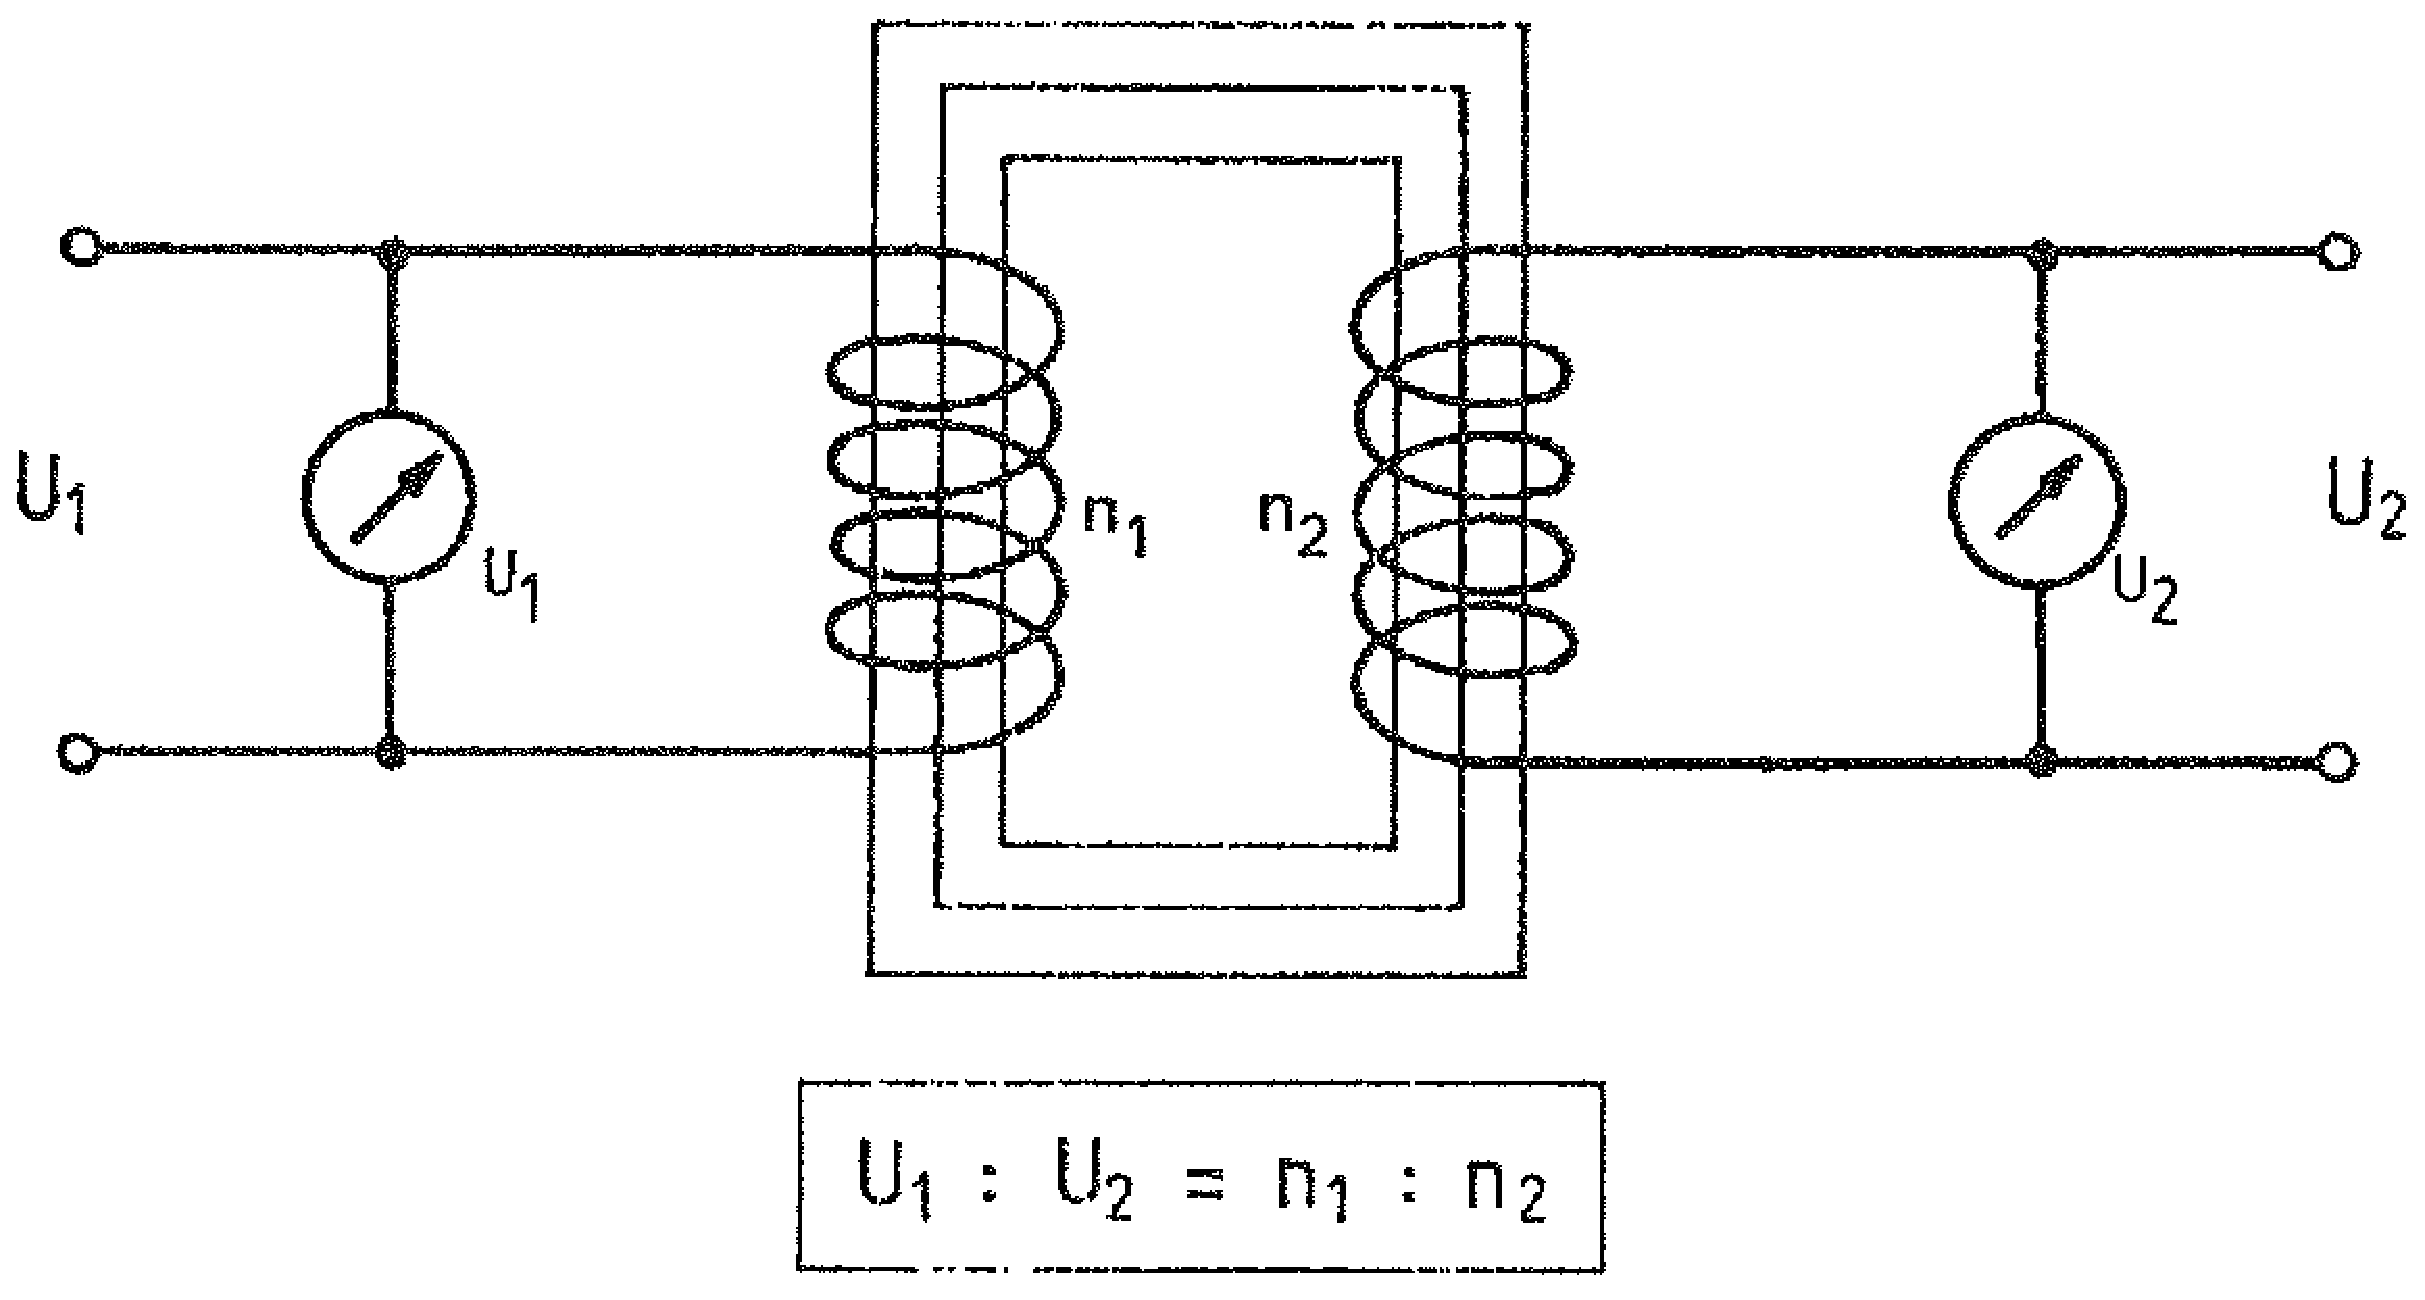
\includegraphics[width=\textwidth]{images/cropped_pdfs/bild_2_2-06.pdf}
\caption{Obelastad transformator}
\label{fig:BildII2-6}
\end{center}
\end{figure*}

I bild \ref{fig:BildII2-6} är transformatorn är obelastad när sekundärkretsen
är bruten.

När primärlindningen ansluts till en växelspänning, induceras det
växelspänningar både över primär- och sekundärlindningarna. Det uppstår även en
ström i primärlindningen, men däremot inte i sekundärlindningen när
sekundärkretsen är bruten. För den obelastade transformatorn gäller sambandet

\(\dfrac{u_1}{u_2} = \dfrac{n_1}{n_2}\)

det vill säga att spänningen över lindningarna är proportionell mot lindningsvarvtalet.

\begin{figure*}[ht]
\begin{center}
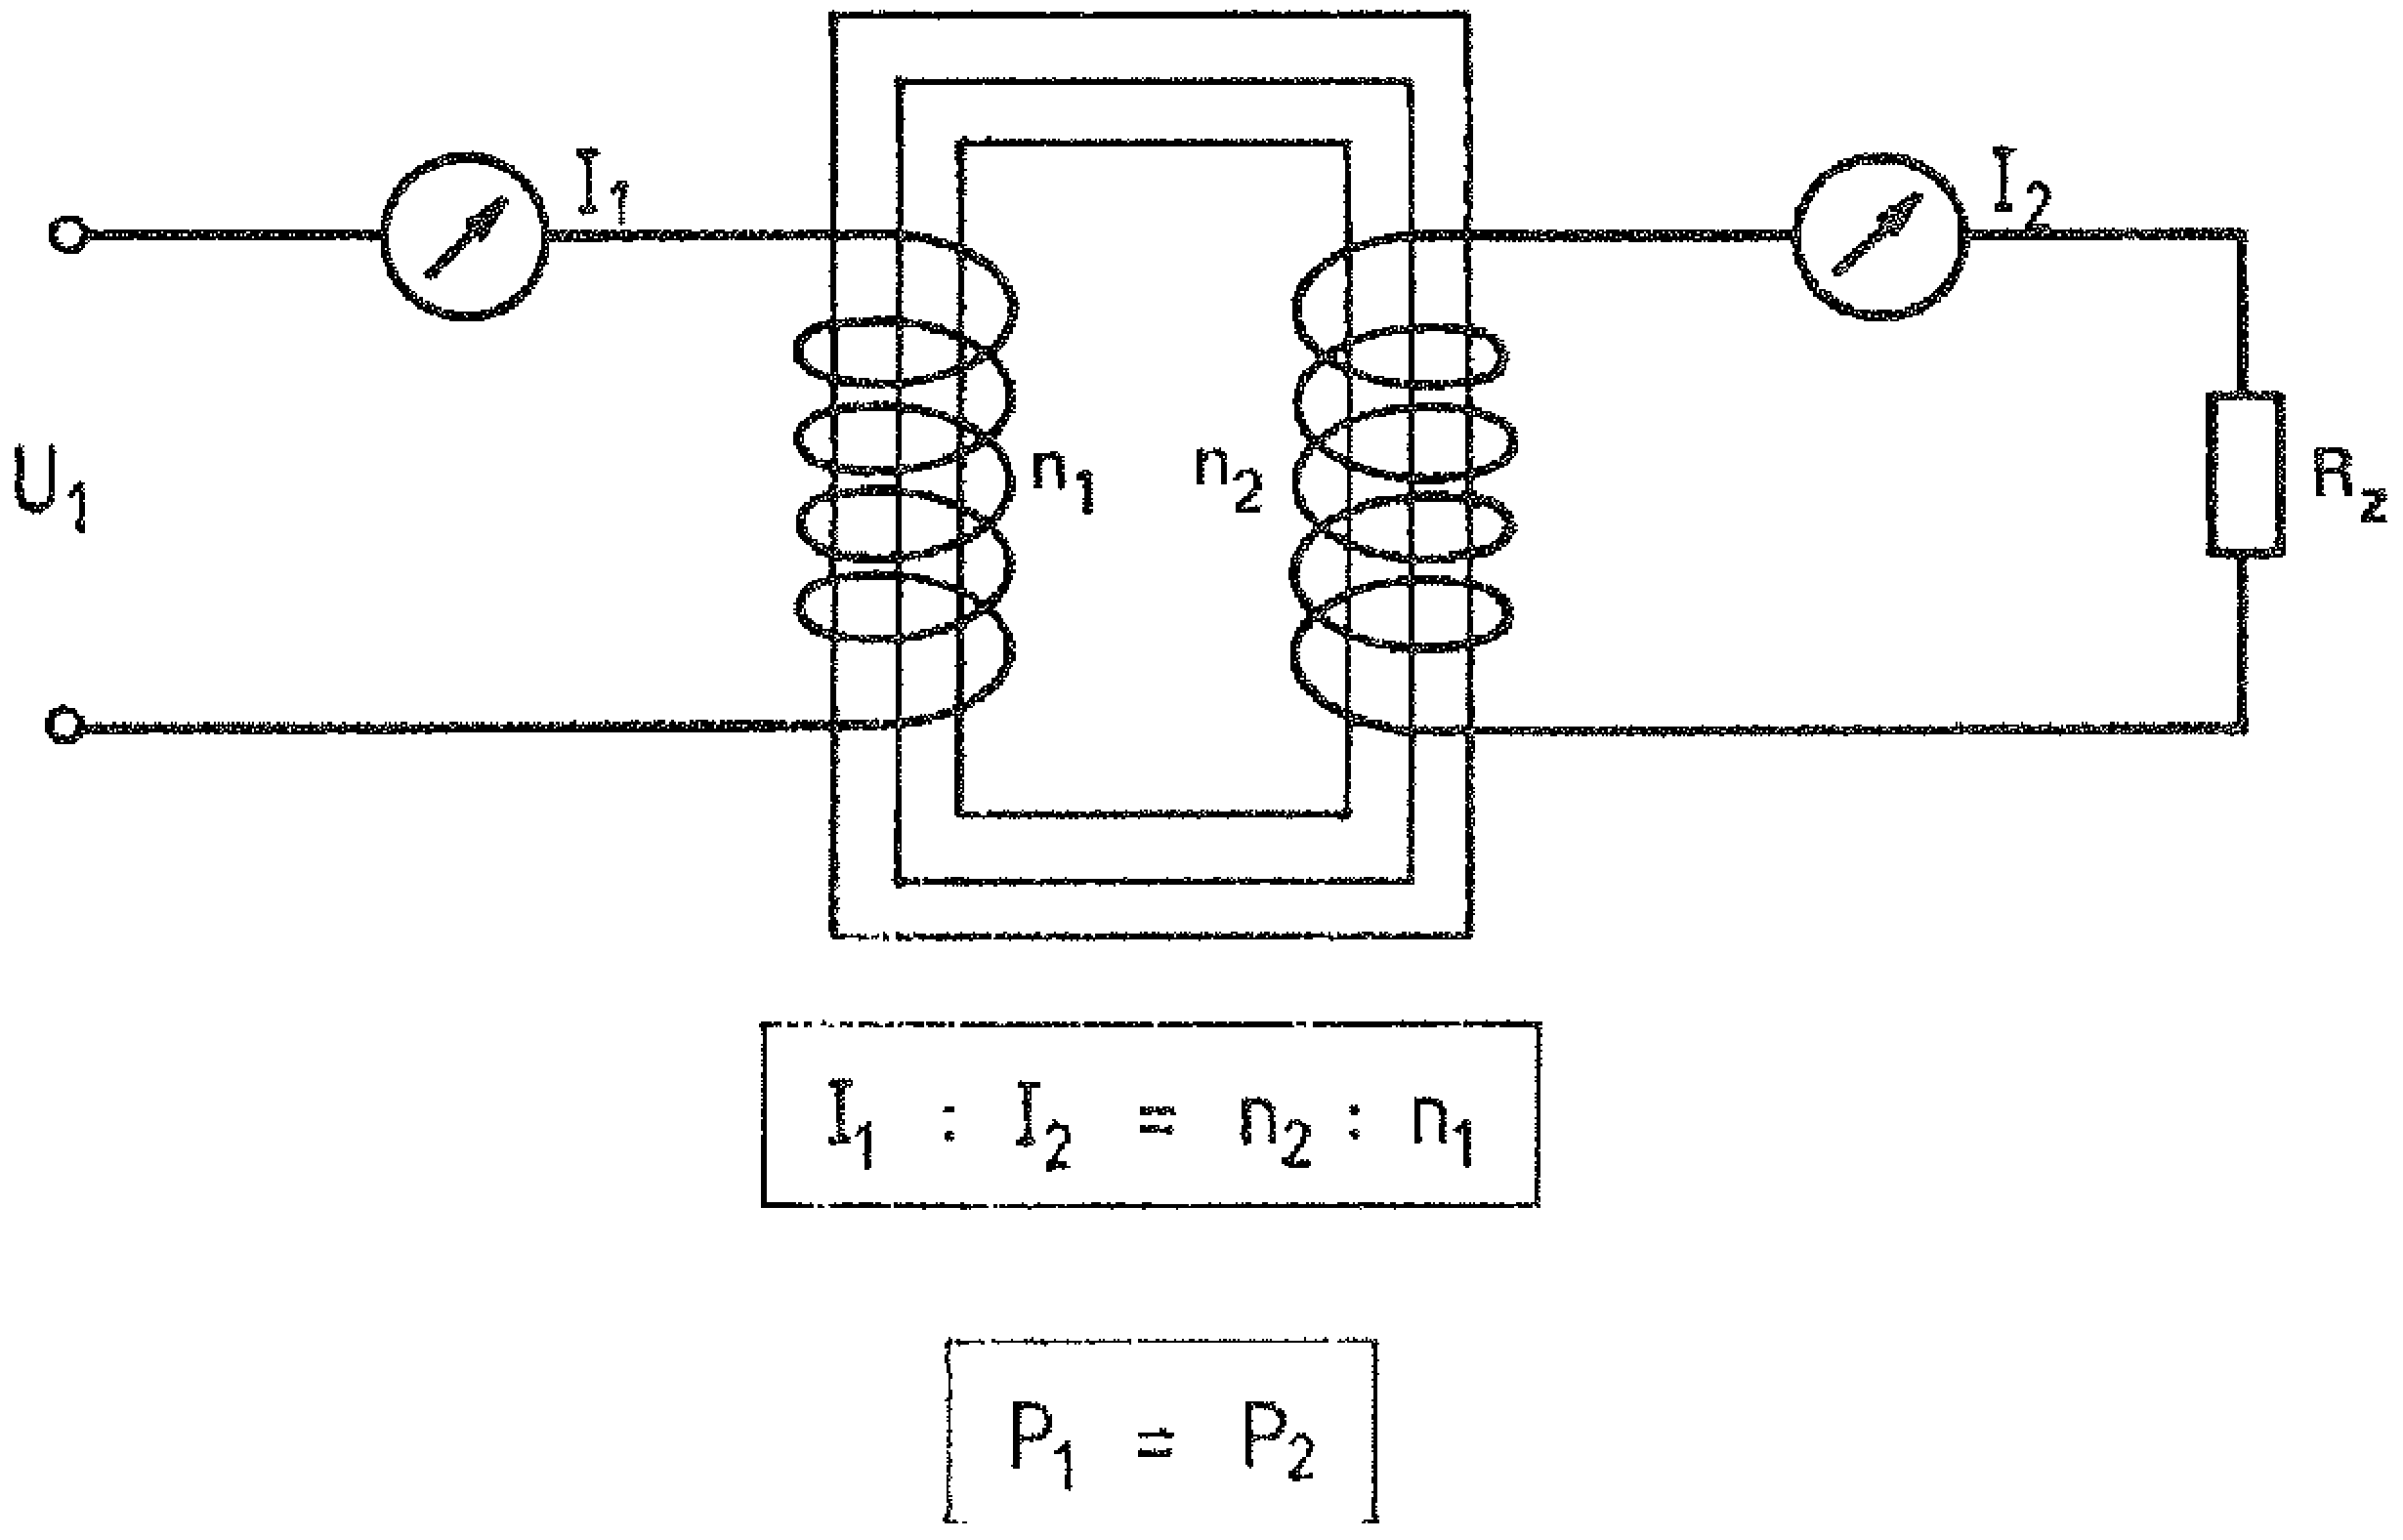
\includegraphics[width=\textwidth]{images/cropped_pdfs/bild_2_2-07.pdf}
\caption{Belastad transformator}
\label{fig:BildII2-7}
\end{center}
\end{figure*}

I bild \ref{fig:BildII2-7} är transformatorn är belastad när sekundärkretsen
är sluten.

När någon av transformatorns sekundärlindningar ingår i en sluten strömkrets,
uppstår en sekundärström där.

Sekundärströmmen alstrar ett magnetfält, som motverkar primärströmmens fält,
hindrar dess växlingar och tar ut energi från primärkretsen.

Strömförbrukningen på primärsidan ökar således i proportion mot
strömförbrukningen på sekundärsidan. Transformatorn reglerar själv hur mycket
energi som den tar från strömkällan och lagrar i fältet för att föra över
till sekundärkretsen.

För den belastade transformatorn gäller, att strömmen genom lindningarna är
omvänt proportionell mot lindningsvarvtalet, dvs. omvänt proportionell mot
varvtalsomsättningen.

\(\dfrac{i_1}{i_2} = \dfrac{n_2}{n_1}\)

Av föregående formler följer att:

\(\dfrac{u_1}{u_2} = \dfrac{i_2}{i_1}\)

Av \(P_1 = u_1 \cdot i_1\) och \(P_2 = u_2 \cdot i_2\) följer att \(P_1 = P_2\).

Om man bortser från förlusterna i transformatorn, så är den effekt som den tar
från kraftkällan lika med den effekt den avger.

Eftersom transformatorn transformerar både spänningar och strömmar så kommer
även impedansen transformeras genom transformatorn.
Denna impedanstransformation följer impedansomsättningen, dvs.

\(\dfrac{Z_1}{Z_2} = \dfrac{n_1^2}{i_2^2}\)

\subsection{Transformatortillämpningar}
\textbf{HAREC a.\ref{HAREC.a.2.4.2.4}\label{myHAREC.a.2.4.2.4}}

\subsubsection{Sparkopplade transformatorer}
\index{galvanisk förbindelse}
\index{spartransformator}
\index{transformator!spar-}

\begin{figure*}[ht]
\begin{center}
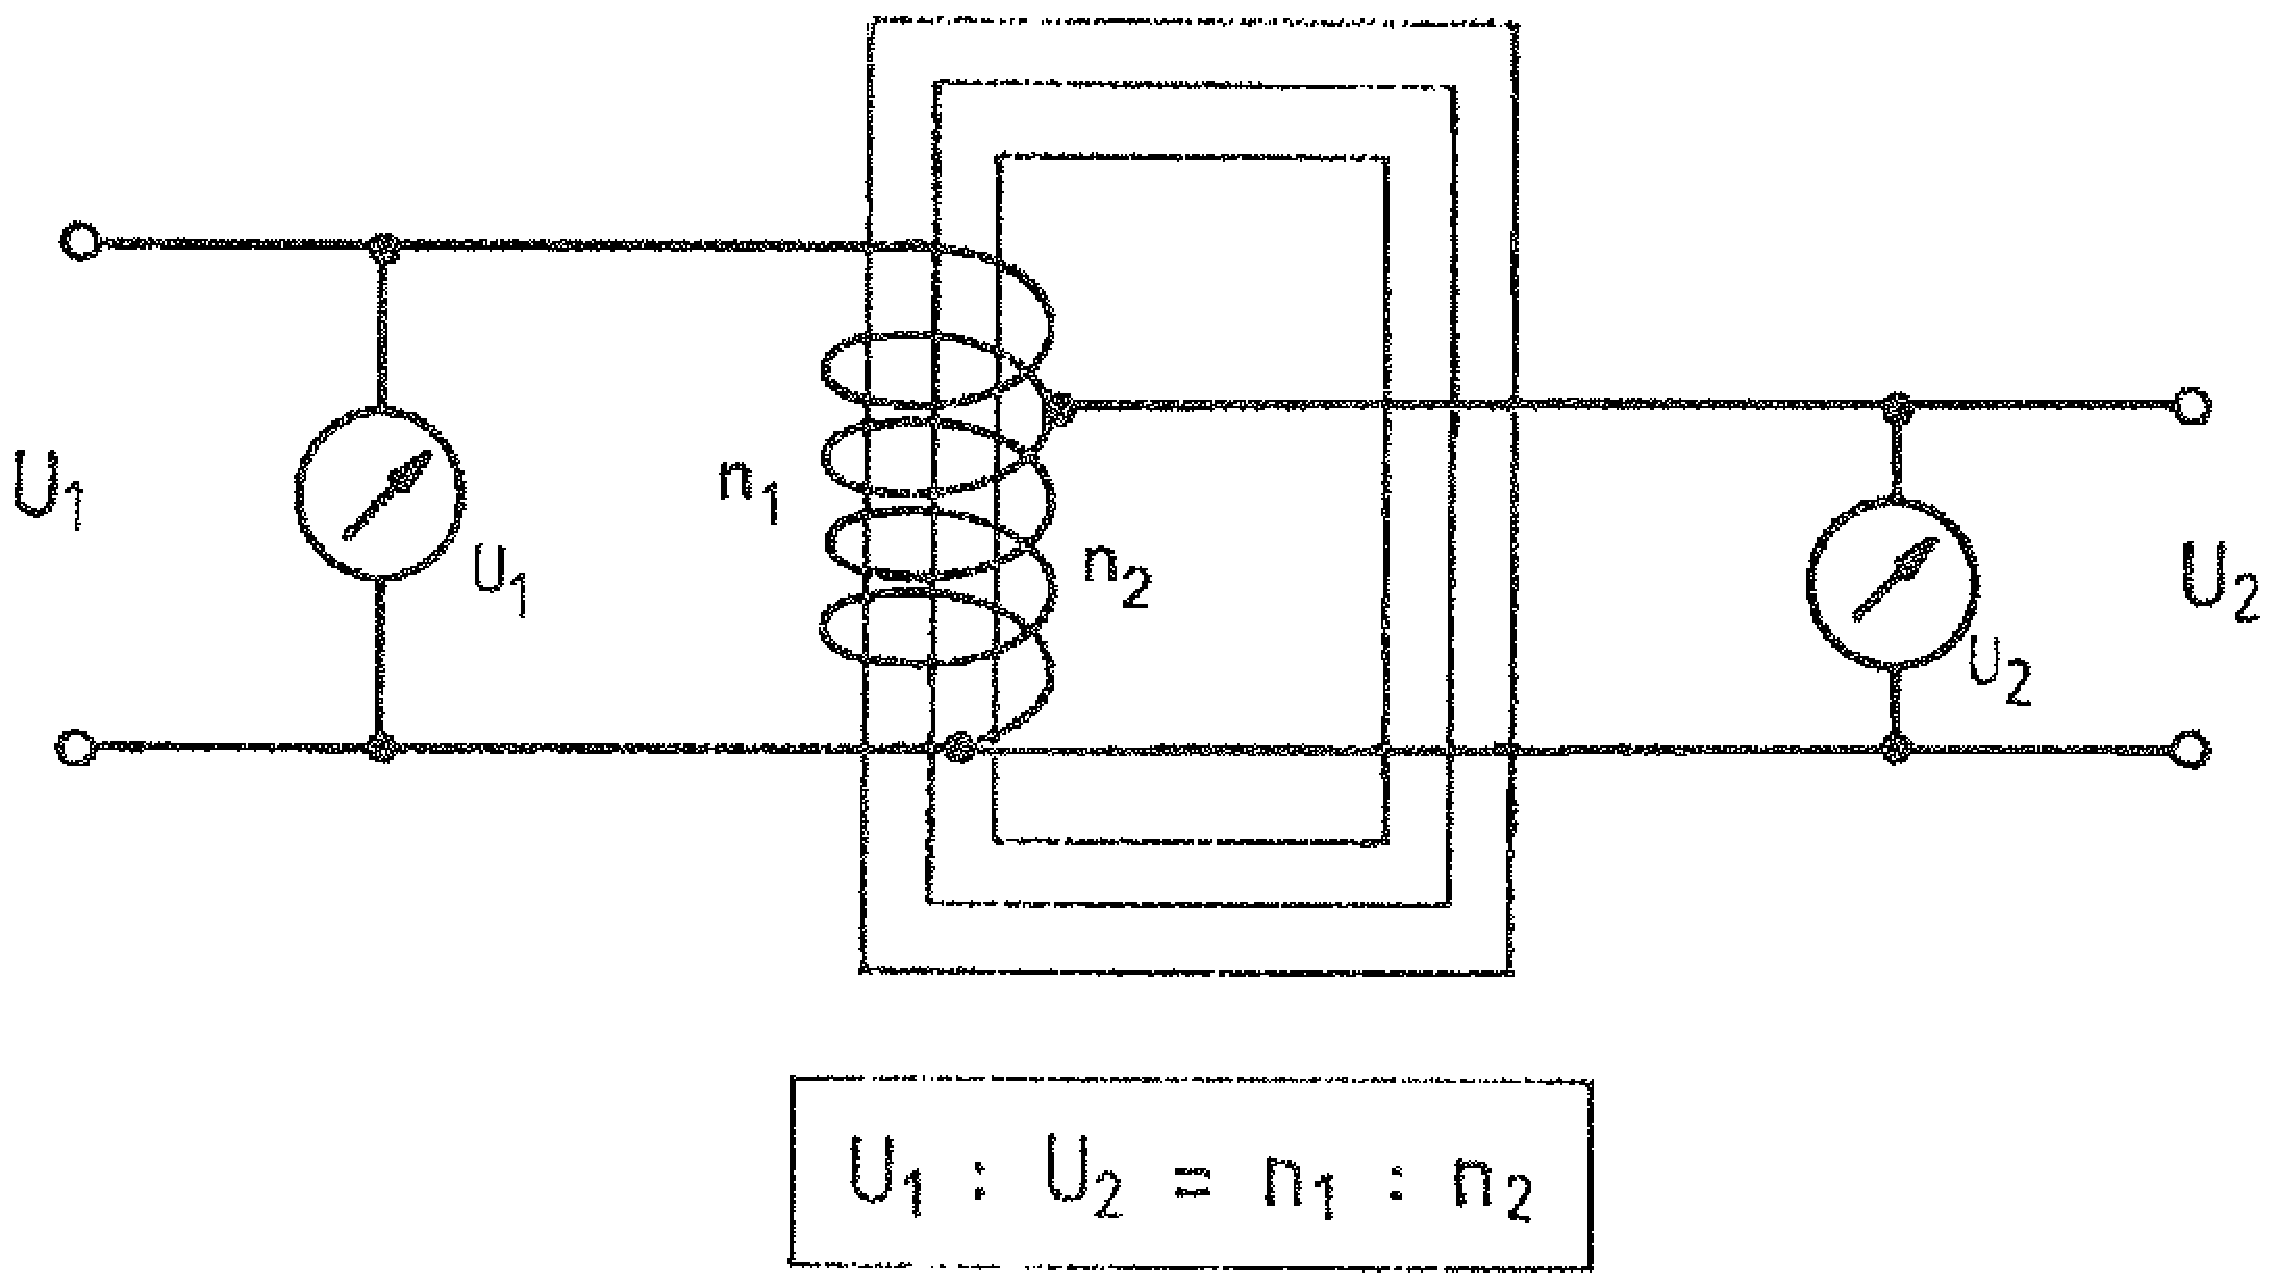
\includegraphics[width=\textwidth]{images/cropped_pdfs/bild_2_2-08.pdf}
\caption{Sparkopplad transformator}
\label{fig:BildII2-8}
\end{center}
\end{figure*}

I bild \ref{fig:BildII2-8} har transformatorn beskrivits så att primär- och
sekundärlindningarnas enda förbindelse med varandra är över ett magnetfält,
alltså utan galvanisk förbindelse.

Varje lindning kan emellertid förses med godtyckliga uttag. Mellan uttagen finns 
då en spänning som är proportionell mot antalet lindningsvarv mellan dessa.

Detta är en metod att spara in på antalet lindningar. För att till exempel omsätta
nätspänningen 230~V till 115~V används ibland en \emph{spartransformator}.

Med en spartransformator kommer olika strömkretsar i galvanisk förbindelse med
varandra och särskild försiktighet ska därför iakttas vid användning av
sparkopplade transformatorer, på grund av risken för elolycksfall.
Spartransformatorer bör därför inte användas i amatörradiosammanhang. Säkrast
är skyddstransformatorer med galvaniskt skilda ledningar och dessutom med speciellt
bra isolering och kapsling.

\subsubsection{Strömtransformatorer}
\index{strömtransformator}
\index{transformator!ström-}

Hög sekundärström under låg sekundärspänning kännetecknar en
\emph{strömtransformator} (eng. \emph{current transformer}),
som illustreras i bild \ref{fig:BildII2-9}.
Strömtransformatorer används i elektriska svetsningsutrustningar,
induktionsugnar osv. Strömtransformatorer används även för mätning av höga
växelströmmar.

\begin{figure*}[ht]
\begin{center}
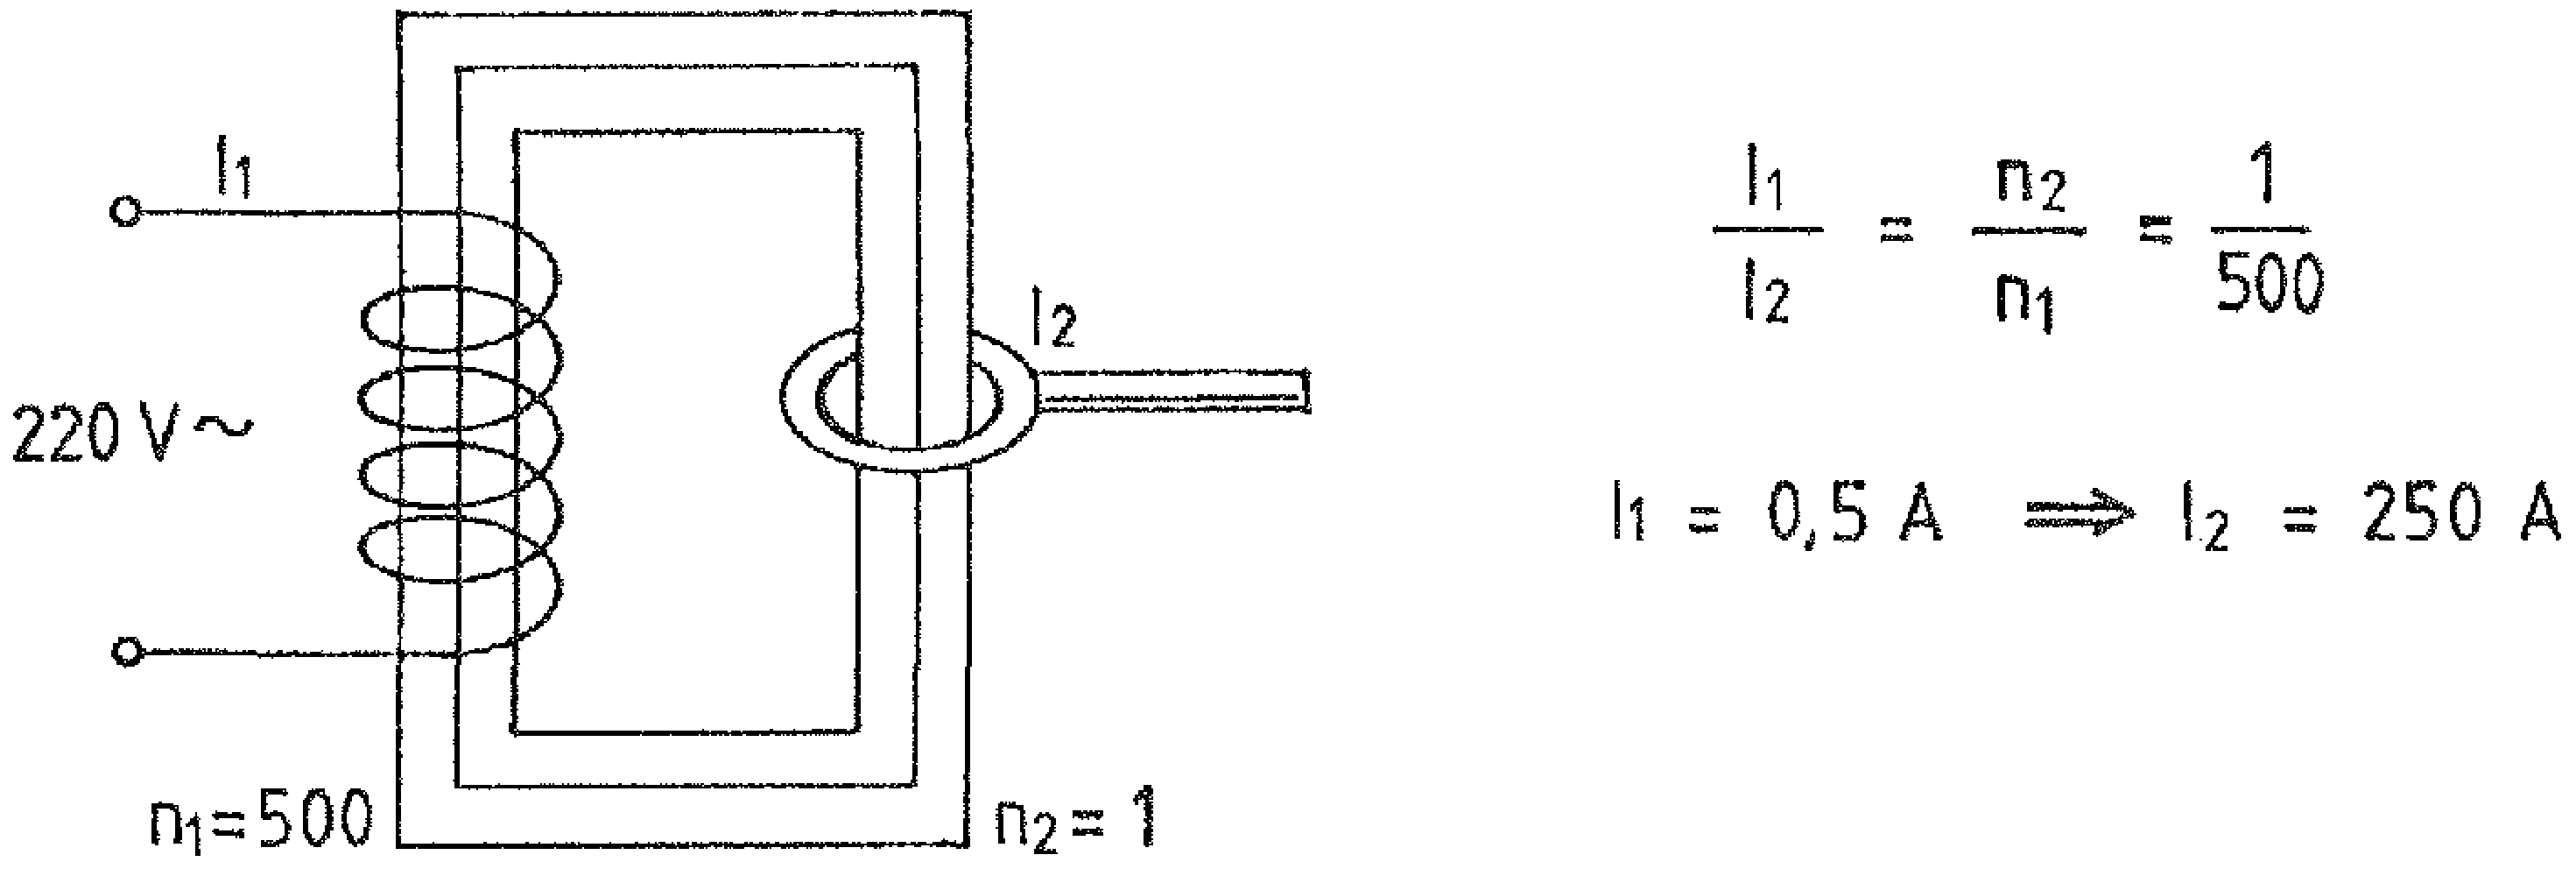
\includegraphics[width=\textwidth]{images/cropped_pdfs/bild_2_2-09.pdf}
\caption{Strömtransformator}
\label{fig:BildII2-9}
\end{center}
\end{figure*}

\subsubsection{Högspänningstransformatorer}
\index{spänningstransformator}
\index{transformator!spännings-}
\index{högspänningstransformator}
\index{transformator!högspännings-}

Hög sekundärspänning under förhållandevis låg sekundärström kännetecknar en
\emph{spänningstransformator} (eng. \emph{voltage transformer}).
Bild \ref{fig:BildII2-10} visar en transformator med ett gnistgap i
sekundärkretsen för tändning av gas.

\emph{Högspänningstransformatorer} (eng. \emph{high voltage transformer})
används i distributionsnät, neonskyltar, tändsystem för förbränningsmotorer,
anodspänningsaggregat för sändare osv.

\begin{figure*}[ht]
\begin{center}
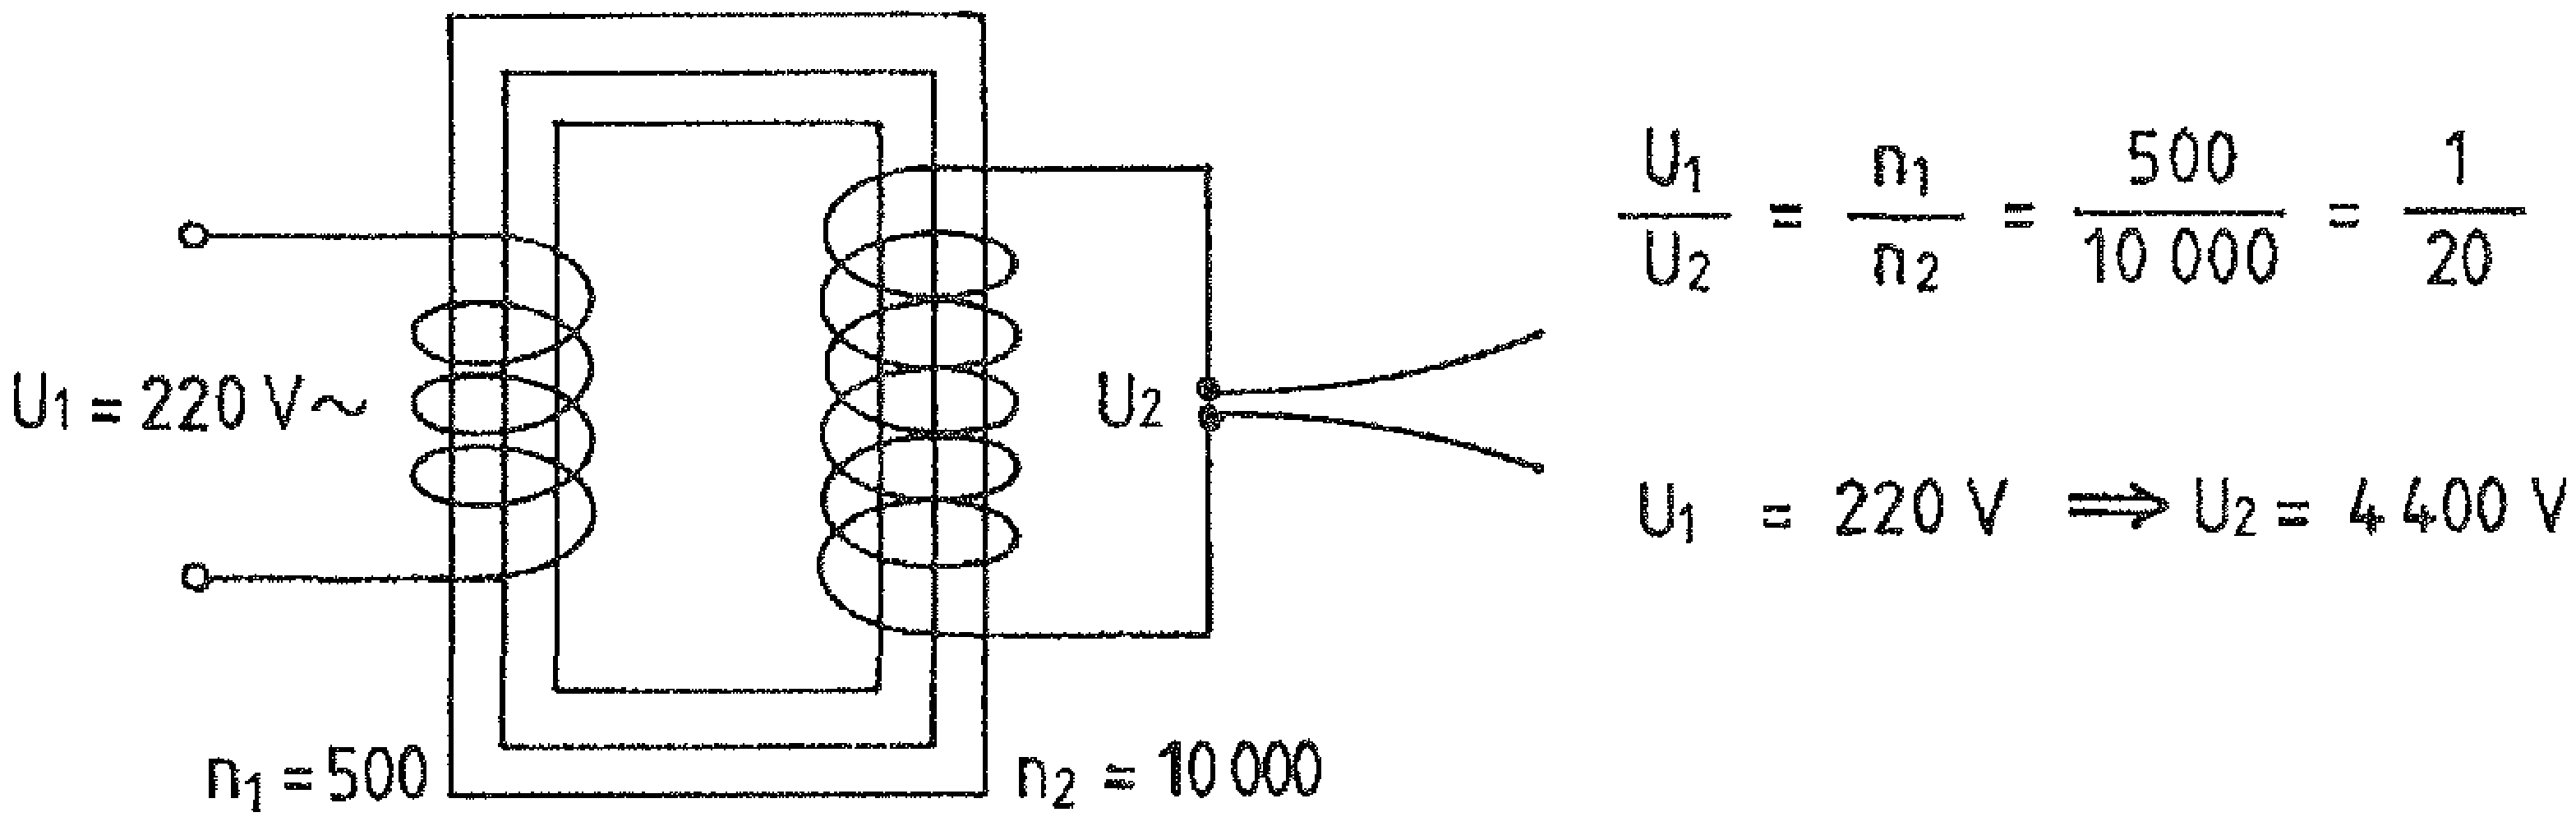
\includegraphics[width=\textwidth]{images/cropped_pdfs/bild_2_2-10.pdf}
\caption{Högspänningstransformator}
\label{fig:BildII2-10}
\end{center}
\end{figure*}

\subsubsection{Låg- och klenspänningstransformatorer}
\index{spänningstransformator}
\index{transformator!spännings-}
\index{lågspänningstransformator}
\index{transformator!lågspännings-}
\index{skyddstransformator}
\index{transformator!skydds-}

\begin{figure*}[ht]
\begin{center}
\includegraphics[width=\textwidth]{images/cropped_pdfs/bild_2_2-11.pdf}
\caption{Klenspänningstransformator}
\label{fig:BildII2-11}
\end{center}
\end{figure*}

Bild \ref{fig:BildII2-11} illustrerar \emph{lågspänningstransformator} (eng.
\emph{low voltage transformer}) som används i lokala distributionsnät,
vanligen med spänningen 400/230~V.

För ökad säkerhet mot elektrisk chock krävs dock att vissa
apparater drivs med en s.k. klenspänning av högst 50~V över en s.k.
\emph{skyddstransformator} (eng. \emph{protection transformer}) med förstärkt
isolering.

\subsection{Sambandet mellan varvtal och impedans}
\textbf{HAREC a.\ref{HAREC.a.2.4.2.3}\label{myHAREC.a.2.4.2.3}}
\index{impedans!transformator varvtal}
\index{impedansomsättning}
\index{transformator!impedansomsättning}
\index{impedanstransformator}
\index{transformator!impedans-}

Transformatorn kan även användas för anpassning av impedanser.
Impedansen Z i en lindning är proportionell mot kvadraten av dess
lindningsvarvtal n.

Om effekten i sekundärlindningen är lika stor som i primärlindningen, gäller
formeln

\(\dfrac{Z_p}{Z_s} = \dfrac{n_p^2}{n_s^2}\)

\section{Halvledardioden}
\textbf{HAREC a.\ref{HAREC.a.2.5}\label{myHAREC.a.2.5}}
\index{halvledardiod}
\index{diod}

\subsection{Allmänt}
I en strömkrets kan av olika anledningar ström tillåtas att flyta i en riktning
men kanske inte i den motsatta. En anordning med en sådan funktion kallas för
diod.

Först bestod en diod av två elektroder i vakuum (se avsnitt
\ref{vakuumdioden}). Därav namnet vakuumdiod.
Numera består en diod oftast av någon halvledare. Därav namnet halvledardiod.

\begin{figure}
\includegraphics[width=\textwidth]{images/cropped_pdfs/bild_2_2-12.pdf}
\caption{Spärrskiktet i en halvledardiod}
\label{fig:BildII2-12}
\end{figure}

Bild \ref{fig:BildII2-12} överst

En halvledardiod består av ett P-ledande och ett N-ledande materialskikt som
fogats samman.

Mellan de båda skikten utbildas ett tunt gränsskikt, som inte innehåller
laddningsbärare. Detta skikt kan vara ledande eller icke ledande -- ett
spärrskikt -- beroende på polariseringen.

\subsection{Halvledardiodens karaktär}
\textbf{HAREC a.\ref{HAREC.a.2.5.1.2}\label{myHAREC.a.2.5.1.2}}

\emph{Framström, temperatur, förlusteffekt, passriktning}

Bild \ref{fig:BildII2-12} mitten

Förbinder man den positiva polen på en spänningskälla med P-skiktet i en diod
och den negativa polen med N-skiktet så är dioden polariserad i passriktningen.
Spärrskiktet upplöses då och ström flyter genom dioden. Elektronerna flyter till
den positiva polen och hålen till den negativa polen.

\emph{Backspänning, backström, läckström, spärriktning}

Bild \ref{fig:BildII2-12} underst

Förbinder man i stället den negativa polen på en spänningskälla med P-skiktet i
en diod och den positiva polen med N-skiktet så är dioden polariserad i
spärriktningen. Spärrskiktet blir då ännu kraftigare.

Endast en obetydlig ström \(I_{SP}\) flyter genom dioden i den s.k.
spärriktningen även vid ökande spänning \(U_{SP}\). Men över en viss spänning
ökar strömmen snabbt -- den s.k. zenereffekten uppstår. Dioden kan då lätt
förstöras av en alltför hög ström.

\begin{figure}
\includegraphics[width=\textwidth]{images/cropped_pdfs/bild_2_2-13.pdf}
\caption{Halvledardiodens karaktäristik}
\label{fig:BildII2-13}
\end{figure}

Bild \ref{fig:BildII2-13}

Strömmen \(I_D\) börjar att flyta när spänningen \(U_D\) har nått ett
tröskelvärde (vid kiseldioder 0,6~V). När spänningen ökar ytterligare däröver,
så ökar även strömmen.

\begin{wrapfigure}[13]{R}{0.5\textwidth}
\includegraphics[width=0.5\textwidth]{images/cropped_pdfs/bild_2_2-14.pdf}
\caption{Schemasymboler för dioder}
\label{fig:BildII2-14}
\end{wrapfigure}

Produkten av spänningsfallet över dioden och strömmen genom den kallas
förlusteffekt. Denna värmer upp dioden. Vid för hög temperatur förstörs
kristallstrukturen. En kiselkristall kan klara upp till 200~°C medan en
germaniumkristall bara klarar 75~°C.

Bild \ref{fig:BildII2-14}

\subsection{Diodtillämpningar}
\textbf{HAREC a.\ref{HAREC.a.2.5.1.1}\label{myHAREC.a.2.5.1.1}}

Likriktning är det vanligaste tillämpningen (se kapitel \ref{kraftaggregat}).
Halvledardioder görs även för en rad andra ändamål och finns i en mängd
utföranden, såsom

\subsubsection{Dioder för spänningsstabilisering (zenerdiod).}
\index{zenerdiod}
\index{diod!zener}

  Inom ett visst område är spänningsfallet över en zenerdiod i en strömkrets
  i det närmaste konstant medan strömmen varierar. Denna egenskap kallas
  zenereffekt och används för konstanthållning av spänning.

  Det finns zenerdioder många olika spänningar och effekter.

\subsubsection{Dioder som variabel kondensator, s.k. kapacitansdiod (VariCap).}
\label{varicap}
\index{varicap}
\index{diod!varicap}

  När en diod är polariserad i spärriktningen så bildas det ett spärrskikt.
  Olika polariseringsspänning alstrar olika tjocka spärrskikt En spärrad diod
  har på så sätt egenskaper som liknar dem i en variabel kondensator. Det finns
  därför dioder där reglerbarheten av kapacitansen är speciellt utvecklad.

\subsubsection{Lysdioder (LED).}
\index{lysdioder}
\index{diod!lysdiod}
\index{LED}
\index{diod!LED}

  Energi frigörs i spärrzonen i en diod som är polariserad i passriktningen. Det
  sker genom rekombination av par av laddningsbärare, varvid det normalt avgår
  energi i form av värme. Vid en viss inblandning av främmande atomer avgår
  istället ljus. Spänningfallet över en lysdiod är ungefär dubbelt så stort som
  över en kiseldiod, d.v.s. ungefär 1,5~volt. Strömmen är i proportion med
  önskad ljusstyrka och mellan 10 och 50~mA.

  \hilight{TODO:  här borde vi även ta upp moderna powerledar som kräver
  konstantströmsmatning, har betydligt högre framspänningsfall m..
  Dessa är ju billiga och populära för experiment. // Hans}

\subsection{Vakuumdioden jämfört halvledardioden}

\begin{figure}
\includegraphics[width=\textwidth]{images/cropped_pdfs/bild_2_2-15.pdf}
\caption{Dioders polarisering i kretsen}
\label{fig:BildII2-15}
\end{figure}

Bild \ref{fig:BildII2-15}

Bilden visar principen för hur de båda diodtyperna ingår i en strömkrets. Den
stora skillnaden är att arbetsspänningen för en vakuumdiod är mångfalt högre än
den för en halvledardiod samt att vakuumdiodens ena elektrod (katoden) behöver
hettas upp för att avge elektroner.

\section{Transistorn}
\textbf{HAREC a.\ref{HAREC.a.2.6}\label{myHAREC.a.2.6}}
\label{transistorn}
\index{transistor}

\subsection{Allmänt}

\begin{wrapfigure}[12]{R}{0.5\textwidth}
\includegraphics[width=0.5\textwidth]{images/cropped_pdfs/bild_2_2-16.pdf}
\caption{Schemasymboler}
\label{fig:BildII2-16}
\end{wrapfigure}

En transistor består av skikt av halvledarelement som sammanfogats. Vanligt är
två N-skikt och ett mellanliggande P-skikt (NPN-transistor) eller två P-skikt och
ett mellanliggande N-skikt (PNP-transistor). Skikten är försedda med
anslutningar.

Bild \ref{fig:BildII2-16}

Vanliga transistortyper
\begin{itemize}
\item NPN-transistorer (bipolära)
\item PNP-transistorer (bipolära)
\item FET-transistorer (fälteffekt-)
\end{itemize}

\subsection{NPN-transistorer}
\textbf{HAREC a.\ref{HAREC.a.2.6.1b}\label{myHAREC.a.2.6.1b}}
\index{NPN-transistor}
\index{transistor!NPN}

Halvledarskikten kallas
\begin{itemize}
\item E emitter
\item B bas
\item C kollektor
\end{itemize}

\begin{wrapfigure}{R}{0.5\textwidth}
\begin{center}
\includegraphics[width=0.1\textwidth]{images/cropped_pdfs/bild_2_6-37.pdf}
\end{center}
\caption{Transistor}
\label{fig:BildII2-17a}
\end{wrapfigure}

Bild \ref{fig:BildII2-17a}

\emph{Spärrzonerna}

\begin{wrapfigure}{R}{0.5\textwidth}
\includegraphics[width=0.5\textwidth]{images/cropped_pdfs/bild_2_2-17.pdf}
\caption{Skikten i en bipolär transistor}
\label{fig:BildII2-17}
\end{wrapfigure}

Bild \ref{fig:BildII2-17} överst

Mellan skikten B och E respektive mellan B och C bildas zoner, vars
ledningsförmåga kan styras elektriskt över anslutningarna.

Bild \ref{fig:BildII2-17} mitten

\emph{Spänningskällan \(U_{BE}\)}

Mellan bas och emitter finns en diodsträcka. När en positiv spänning läggs på
basen och en negativ spänning på emittern, så polariseras diodsträckans spärrzon
i passriktningen. Spärrzonen upplöses då och det flyter en s.k. basström
\(I_B\).

Bild \ref{fig:BildII2-17} nederst

\emph{Spänningskällan \(U_{CE}\)}

När en positiv spänning läggs på kollektorn och en negativ spänning läggs på
emittern, så polariseras diodsträckan i spärriktningen. Spärrzonen förstärks då
och det flyter ingen ström.

Bild \ref{fig:BildII2-18}

\emph{Inverkan av både \(U_{BE}\) och \(U_{CE}\)}

Två spänningskällor \(U_{BE}\) och \(U_{CE}\) ansluts till en emitterkopplad NPN-transistor.
Ur den starkt dopade emitterzonen strömmar elektronerna in i den svagt dopade
baszonen (spänning: \(U_{BE}\)). De flesta elektronerna blir emellertid inte
kvar i basen. De stöter igenom det tunna basskiktet och når fram till
kollektorskiktet med spänningen \(U_{CE}\). Det flyter en kollektorström.

För strömmen \(I_E\) (emitterström), \(I_B\) (basström) och \(I_C\)
(kollektorström) gäller:

\(I_E = I_B + I_C\) där \(I_B \ll I_C\) (\(\ll\) mycket mindre än)

Kollektorströmmen \(I_C\) kan styras med basspänningen \(U_{BE}\).

En liten ändring i basspänningen ger stor förstärkande verkan i
kollektorströmmen.

\begin{figure}
\includegraphics[width=\textwidth]{images/cropped_pdfs/bild_2_2-18.pdf}
\caption{Emitterkopplad transistor}
\label{fig:BildII2-18}
\end{figure}

\subsection{Förstärkningsfaktor}
\textbf{HAREC a.\ref{HAREC.a.2.6.2}\label{myHAREC.a.2.6.2}}
\index{förstärkningsfaktor!transistor}
\index{transistor!förstärkningsfaktor}

Om strömmen i ingångskretsen för en transistor ändras, så kan strömmen i
utgångskretsen ändras mer. Det blir då en förstärkning.

Av sambandet \(I_C = f(I_B)\) framgår strömförstärkningsfaktorn \(\beta\) eller
\(h_{FE}\) som är kvoten av ändringen i utgångsströmmen och i ingångsströmmen i
transistorns aktiva (linjära) område.

\begin{figure}
\includegraphics[width=\textwidth]{images/cropped_pdfs/bild_2_2-19.pdf}
\caption{Karaktäristika för transistor BC 107}
\label{fig:BildII2-19}
\end{figure}

Bild \ref{fig:BildII2-19}

För emitterkoppling gäller:

\(h_{FE} = \dfrac{∆I_C}{∆I_B}\)

\begin{tabular}{ll}
  \(h_{FE}\) & strömförstärkningsfaktorn \\
  \(∆I_c\)   & ändringen i kollektorströmmen \\
  \(∆I_B\)   & ändringen i basströmmen \\
\end{tabular}

\subsection{PNP-transistorer}
\textbf{HAREC a.\ref{HAREC.a.2.6.1a}\label{myHAREC.a.2.6.1a}}
\index{PNP-transistor}
\index{transistor!PNP}

Ersätter man de två N-skikten i en NPN-transistor med P-skikt och P-skiktet med
ett N-skikt så erhåller man en PNP-transistor.

Uppbyggnad, koppling och användning av en PNP-transistor motsvarar i övrigt den
för en NPN-transistor. Spänningskällorna måste emellertid ha motsatt polaritet.

\subsection{Fälteffekttransistorer}
\textbf{HAREC a.\ref{HAREC.a.2.6.3}\label{myHAREC.a.2.6.3}}
\index{fälteffekttransistor}
\index{transistor!fälteffekt}
\index{FET}
\index{transistor!FET}

\emph{Allmänt}

Fälteffekttransistorer (förkortat FET) har mycket hög ingångsimpedans och
styrströmmen blir därför mycket svag. Man säger därför att en FET är
spänningsstyrd.

Även NPN- och PNP-transistorer -- kallade bipolära transistorer -- styrs med
spänning, men dessa typer har en relativt lågt ingångsimpedans och därför högre
styrström. Man säger därför att de är strömstyrda.

\begin{wrapfigure}[6]{R}{0.5\textwidth}
\includegraphics[width=0.5\textwidth]{images/cropped_pdfs/bild_2_2-20.pdf}
\caption{Schemasymbol för en FET}
\label{fig:BildII2-20}
\end{wrapfigure}

Bild \ref{fig:BildII2-20}

Fälteffekttransistorn har tre anslutningar (elektroder):

\begin{tabular}{ll}
  S & source (katod) \\
  D & drain (anod) \\
  G & gate (grind, styre) \\
\end{tabular}

\begin{wrapfigure}{R}{0.5\textwidth}
\includegraphics[width=0.5\textwidth]{images/cropped_pdfs/bild_2_2-21.pdf}
\caption{Skikten i en N-kanal FET}
\label{fig:BildII2-21}
\end{wrapfigure}

\emph{Fälteffekttransistorns uppbyggnad}

Bild \ref{fig:BildII2-21}

Bilden visar ett N-ledande skikt (även kallat N-kanal) med elektroderna S och D
anslutna till respektive ändar av skiktet. N-kanalen passerar mellan två
P-ledande skikt förbundna med styrelektroden G.

När en spärrspänning läggs mellan G och S, så breder spärrskikten ut sig och
N-kanalen blir trängre. Läggs en negativ spänning på S och en positiv spänning
på D, så kommer det att flyta en ström i N-kanalen. Strömmens styrka kan
påverkas med spänningen på G.

En liten spänningsändring \(∆U_{GS}\) medför stor ändring av strömmen
\(∆I_{GS}\) i N-kanalen. Detta innebär förstärkning.

\begin{wrapfigure}{R}{0.5\textwidth}
\includegraphics[width=0.5\textwidth]{images/cropped_pdfs/bild_2_2-22.pdf}
\caption{Skikten i en N-kanal MOSFET}
\label{fig:BildII2-22}
\end{wrapfigure}


Bild \ref{fig:BildII2-22}

\index{MOSFET}
\index{transitor!MOSFET}

I en Metal Oxide Semicoductor Field Effect Transistor (MOSFET) är
G-elektroden isolerad med ett kiseloxidskikt, trots att namnet förespeglar
ett metalloxidskikt. Funktionssättet är samma som för en FET.
Drain-strömmen kan ökas eller minskas med hjälp av en
positiv respektive negativ spänning på G.
%\url{https://en.wikipedia.org/wiki/MOSFET}

\emph{Resistansen mellan gate och source}

För att erhålla en förstärkning med en FET, sätter man in en resistor
\(R_0\) i drain-strömkretsen. Över resistorn uppstår då spänningsändringar i
proportion med strömändringarna.

För att fastställa viloströmmen och därmed arbetspunkten för samma transistor
sätter man in en resistor \(R_S\) i source-strömkretsen. storleken på
source-resistorn ger sig av önskad gate-förspänning \(-U_{GS}\).

\(R_S = \dfrac{-U_{GS}}{I_D}\)

\subsection{Sambandet drain-ström och spänning}

\begin{wrapfigure}{R}{0.5\textwidth}
\includegraphics[width=0.5\textwidth]{images/cropped_pdfs/bild_2_2-23.pdf}
\caption{Karaktäristik för N-kanal FET}
\label{fig:BildII2-23}
\end{wrapfigure}

Bild \ref{fig:BildII2-23}

För att beskriva en FET använder man sig av karaktäristiska kurvor. Vi har redan
presenterat bipolära transistorers in- och utgångsegenskaper i kurvform.
Eftersom ingångsströmmen (gateströmmen) i en FET är praktiskt taget noll, så är
en sådan kurva utan praktisk mening. I stället framställer man grafiskt
sammanhanget mellan styrspänningen \(U_{GS}\) och utgångsströmmen (drainströmmen
\(I_D\)). Eftersom det finns N-kanal FET och P-kanal FET så skiljer polariteten
på \(U_{GS}\) för dessa båda typer.

\section{Elektronrör}
\label{elektronrör}
\index{elektronrör}

\subsection{Allmänt}

Ett elektronrör består av två eller flera elektroder i en lufttom glaskolv.

\subsection{Vakuumdioden (tvåelektrodröret)}
\textbf{HAREC a.\ref{HAREC.a.2.8.1}\label{myHAREC.a.2.8.1}}
\label{vakuumdioden}
\index{vakuumdioden}
\index{elektronrör!diod}
\index{anod}
\index{katod}

\begin{wrapfigure}[9]{R}{0.5\textwidth}
\includegraphics[width=0.5\textwidth]{images/cropped_pdfs/bild_2_2-24.pdf}
\caption{Schemasymboler för dioder}
\label{fig:BildII2-24}
\end{wrapfigure}

Bild \ref{fig:BildII2-24}

Dioden innehåller två elektroder anod (a) och katod (k), med f där
f = glödtråd (filament).

\emph{Anoden} ska dra elektronerna från katoden.
\emph{Katoden} ska avge elektronerna och måste därför hettas upp.

Upphettningen av katoden görs antingen med direkt upphettning, d.v.s. katoden
är i sig själv en glödtråd, där en 4- till 6-volts strömkälla är vanligt, eller
med indirekt upphettning, d.v.s. en glödtråd omsluter och hettar upp ett
speciellt katodmaterial, där en 1,5 till 12,6~volts glödströmkälla är vanligt.

\subsubsection{Edisoneffekten}
\index{Edisoneffekten}
\index{elektronrör!Edisoneffekten}

\begin{wrapfigure}[12]{R}{0.5\textwidth}
\includegraphics[width=0.5\textwidth]{images/cropped_pdfs/bild_2_2-25.pdf}
\caption{Edisoneffekten}
\label{fig:BildII2-25}
\end{wrapfigure}

Bild \ref{fig:BildII2-25} illustrerar \emph{Edisoneffekten}, dvs. när katoden
upphettas lossnar fria elektroner från den och bildar ett moln.
Med en spänning mellan anod och katod, med anoden positiv, så kommer
elektronerna att dras mot anoden.
En s.k. anodström börjar att flyta.

\subsubsection{\(I_a/U_a\)-karaktäristikan för en vakuumdiod}

\begin{figure}
\includegraphics[width=\textwidth]{images/cropped_pdfs/bild_2_2-26.pdf}
\caption{Diodens karaktäristik}
\label{fig:BildII2-26}
\end{figure}

Bild \ref{fig:BildII2-26} illustrerar rördiodesn karakteristik.
När anoden ges positiv potential (anodspänning), flyter en elektronström från
katod till anod (anodström).
Om anodspänningen \(U_a\) ökar så ökar anodströmmen \(I_a\).
Varje par av talvärden representerar en punkt i ett diagram, som det på bilden.
När anodspänningen ökat till ett visst värde, så ökar inte anodströmmen
ytterligare.
I ett mellanområde är kurvan i det närmaste rak.

\subsubsection{Likriktarverkan}
\index{elektronrör!likriktarverkan}

När anoden i en vakuumdiod ges positiv potential i förhållande till katoden,
flyter en s.k. anodström förutsatt att katoden upphettas så att den avger fria
elektroner.

När anoden ges en negativ potential i förhållande till katoden flyter däremot
ingen anodström.

Vakuumdioden kan därför användas för likriktning av växelströmmar. Den har en
likriktande funktion.

\subsubsection{Halvvågslikriktning.}

\begin{figure}
\includegraphics[width=\textwidth]{images/cropped_pdfs/bild_2_2-27.pdf}
\caption{Halvvågslikriktning}
\label{fig:BildII2-27}
\end{figure}

Bild \ref{fig:BildII2-27} illustrerar halvvågslikriktning.
När anoden ges en omväxlande positiv och negativ potential, en växelspänning, så
flyter anodström under varje positiv halvperiod av växelspänningen.
En likströmspuls uppstår under varannan halvperiod.

\subsubsection{Helvågslikriktning.}

\begin{figure}
\includegraphics[width=\textwidth]{images/cropped_pdfs/bild_2_2-28.pdf}
\caption{Helvågslikriktning}
\label{fig:BildII2-28}
\end{figure}

Bild \ref{fig:BildII2-28} illustrerar halvvågslikriktning.
Med ett elektronrör med dubbla anoder och en transformator med mittuttag på
sekundärlindningen, kan växelspänningens båda halvperioder utnyttjas så, att
anodström flyter i samma riktning under alla halvperioder.

\begin{figure}
\includegraphics[width=\textwidth]{images/cropped_pdfs/bild_2_2-29.pdf}
\caption{Likriktande funktion}
\label{fig:BildII2-29}
\end{figure}

Bild \ref{fig:BildII2-29} illustrerar hur växelspännng via två
två halvvågslikriktningar formar en helvågslikriktning.

\subsection{Vakuumtrioden (treelektrodröret)}
\index{vakuumtrioden}
\index{trioden}
\index{elektronrör!triod}

\begin{figure*}[h]
\begin{center}
  %%\begin{wrapfigure}[9]{R}{0.5\textwidth}
  \includegraphics[width=0.5\textwidth]{images/cropped_pdfs/bild_2_2-30.pdf}
  \caption{Symboler för triod och pentod}
  \label{fig:BildII2-30}
  %%\end{wrapfigure}
\end{center}
\end{figure*}

Bild \ref{fig:BildII2-30} illustrerar symboler för triod och pentod.

Trioden innehåller tre elektroder anod (a), styrgaller (\(g_1\)) och katod (k)
med glödtråd (f = filament).

\subsubsection{Triodens funktion}

Bild \ref{fig:BildII2-31} illustrerar en triod och dess elektronström.
En triod fungerar som en diod, när styrgallret ges samma potential som katoden.
Valet av förspänning avgör triodens arbetssätt. styrgallret kan ges positiv,
neutral eller negativ potential (förspänning) i förhållande till katoden. Med
styrgallret positivt ökar anodströmmen. Med gallret negativt minskar den.

Trioden har en \emph{förstärkande} funktion eftersom anodströmmen kan styras med
styrgallret. En liten ändring av gallerspänningen medför stor ändring av
anodströmmen. Vid positiv förspänning flyter det gallerström, som inte får bli
för hög. Vanligen väljs en negativ förspänning.

\begin{figure}[h]
\includegraphics[width=\textwidth]{images/cropped_pdfs/bild_2_2-31.pdf}
\caption{Elektronstömmen i en triod}
\label{fig:BildII2-31}
\end{figure}

\subsubsection{Triodens strömkretsar och strömkällor}

\begin{tabular}{lll}
Glödströmskrets      & Anodkrets        &  Gallerkrets \\
Glödbatteri          & Anodbatteri      &  Gallerbatteri \\
Glödspänning \(U_f\) & Anodsp. \(U_a\)  &  Gallersp. \(U_{g1}\) \\
Glödström \(I_f\)    & Anodstr. \(I_a\) &  Gallerstr. \(I_{g1}\) \\
\end{tabular}

Vanligen används nätdrivna strömkällor i stället för batterier.

Valet av gallerförspänning är avgörande för triodens arbetssätt.

\subsection{Pentoden (femelektrodröret)}
\index{pentod}
\index{elektronrör!pentod}

Pentaden innehåller fem elektroder.

\begin{tabular}{ll}
  a       & anod \\
  \(g_3\) & bromsgaller \\
  \(g_2\) & skärmgaller \\
  \(g_1\) & styrgaller \\
  k      & katod, med f f = glödtråd (filament) \\
\end{tabular}

Bromsgallret förbinds med katoden. Skärmgallret ges en potential som är något
lägre än anodspänningen. Broms- och skärmgallren förhindrar elektronerna att
studsa tillbaka till styrgallret efter anslaget mot anoden.


\subsection{Tetroden (fyraelektrodröret)}
\index{tetrod}
\index{elektronrör!tetrod}

Denna rörtyp innehåller fyra elektroder. Uppbyggnaden är densamma som pentodens,
men bromsgallret saknas.

\subsection{Karaktäristika för elektronrör}

\begin{figure}
\includegraphics[width=\textwidth]{images/cropped_pdfs/bild_2_2-32.pdf}
\caption{Karaktäristika för elektronrör}
\label{fig:BildII2-32}
\end{figure}

Bild \ref{fig:BildII2-32} illustrerar ett \(I_a/U_{gt}\)-diagram för en triod
eller pentod, vid \(U_a\) = konstant

\begin{wrapfigure}[20]{R}{0.5\textwidth}
\includegraphics[width=0.5\textwidth]{images/cropped_pdfs/bild_2_2-33.pdf}
\caption{Branthet}
\label{fig:BildII2-33}
\end{wrapfigure}

\(I_a/U_a\)-diagram för en triod, vid \(U_{g1}\) = konstant

\(I_a/U_a\)-diagram för en pentod, vid \(U_{g1}\) = konstant

Tre kurvor visas i \(I_a/U_a\)-diagrammen, med olika värden på
\(U_{g1}\) = konstant (\(U_{g1}\) är s.k. parameter).

\subsection{Branthet $S$ och inre resistans $R_i$}

Bild \ref{fig:BildII2-33} visar brantheten.
Om man (vid konstant anodspänning) ändrar gallerförspänningen med värdet
\(\Delta U_{g1}\) så ändrar sig anodströmmen med värdet \(\Delta I_a\).

Branthet \(S = \dfrac{\Delta I_a}{\Delta U_{g1}}\)

\(S\ [mA/V]\) \(\Delta I_a\ [mA]\) \(U_{g1}\ [V]\)

Bild \ref{fig:BildII2-34} visar den inre resistansen.
Om man (vid konstant gallerförspänning) ändrar anodspänningen med
\(\Delta U_a\) så ändras anodströmmen med värdet \(\Delta I_a\).

Inre resistans \(R_i = \dfrac{\Delta U_a}{\Delta I_a}\)

\(R_i\ [k \omega]\)  \(\Delta U_a\ [V]\)  \(\Delta I_a\ [mA]\)

\begin{figure}[h]
\includegraphics[width=\textwidth]{images/cropped_pdfs/bild_2_2-34.pdf}
\caption{Inre resistans}
\label{fig:BildII2-34}
\end{figure}

Om man vill ändra anodströmmen med \(\Delta I_a\), så ges det två möjligheter,
antingen ändra gallerförspänningen med värdet \(\Delta U_{g1}\)
eller ändra anodspänningen med värdet \(\Delta U_a\).
Med ändring av gallerförspänningen med värdet \(U_{g1}\) kan man åstadkomma
samma anodströmsändring \(\Delta I_a\) som med en ändring av anodspänningen
med värdet \(\Delta U_a\).

\subsection{Barkhausens elektronrörsformler}
\index{Barkhausen elektronrörsformler}
\index{elektronrör!Barkhausen formler}

Förstärkningsfaktorn \(\mu \) illustreras av följande samband gäller mellan de s.k. rörkonstanterna

\(\mu = S \cdot R_i\)

\emph{Exempel:}
Beräkna \(\mu\)  om \(S = 2\ mA/V\) \(R = 10\ k\Omega\) \(\mu = ?\)

\emph{Svar:} \(\mu = 20\) (\(\mu\)  är dimensionslös)

\subsection{Transistorer jämfört med elektronrör}

Transistorer har fördelar som lågt pris, små dimensioner, lång livslängd,
enkel strömförsörjning (glödström behövs inte) and låg driftspänning (6~V,
12~V \ldots ). Nackdelen som traditionellt finns är känslighet för
överbelastning och höga temperaturer.

Elektronrör har fördelen av tålighet mot överbelastning, men bland nackdelarna
har man att man behöver hög anodspänning, behöver glödström samt att de är
utrymmeskrävande.

Ett användningsområde, där elektronrör ännu är vanliga, är i större
sändarslutsteg.

Transistorer ersätter numera nästan helt elektronrören, men man bör ändå känna
elektronrörens egenskaper och arbetssätt.

\section{Digitala kretsar}
\index{digitala kretsar}
\label{digitala kretsar}

Särskilt under det senaste decenniet har digital elektronik blivit vanlig i
utrustningar för radio- och telekommunikation. Även inom amatörradio används nu
denna teknik. Ämnet är mycket omfattande. Utvecklingen är att enkla digitala
funktioner snabbt ersätts av komplexa datasystem. Här redogörs endast för några
grundläggande digitala funktioner.

Amatörradions kärna finns ännu i \emph{analogtekniken}, där det under ett
förlopp kan förekomma många olika storheter, t.ex. spänningar mellan noll och
ett högsta värde.

I digitaltekniken förekommer bara ett bestämt antal tillstånd. I det enklaste
digitala systemet finns två tillstånd, t.ex. 0 och 1 eller Till och Från eller
Hög och Låg eller Fel och Rätt osv. Ett system med två tillstånd kallas
binärt. En lampa som tänds eller släcks med en enkel strömställare är ett binärt
system. Strömställaren kan ha olika utföranden. Det kan vara en mekanisk kontakt
som är styrd för hand eller av en reläspole. Det kan också vara en transistor
eller annan anordning.

\subsection{Transistorn som strömställare}

\begin{figure}
\includegraphics[width=\textwidth]{images/cropped_pdfs/bild_2_2-35.pdf}
\caption{Transistorn som analog förstärkare respektive digital strömställare}
\label{fig:BildII2-35}
\end{figure}

Bild \ref{fig:BildII2-35} visar två transistorkopplingar.
Den till vänster är en analog förstärkare för växelspänning.
Om det på grund av en viss basspänning flyter en kollektorström av 1~mA och
kollektorresistorn är 5~k\(\Omega\), så blir spänningsfallet
över den resistorn 5~V. Eftersom matningsspänningen är 12~V, så blir då
spänningen 7~V mellan kollektorn och minus.

Kopplingen till höger fungerar som en binär strömställare. Antag att insignalen
intar ett av två spänningstillstånd, antingen 0~V (låg) eller 5~V (hög). När
inspänningen är t.ex. 5~V, så flyter så mycket basström genom basresistorns
10~k\(\Omega\), att transistorn blir fullt utstyrd.

Därmed är spänningen mellan kollektor och emitter, dvs. utspänningen, nära 0~V
(0,1 till 0,2~V beroende på transistortyp). Man säger då att utgången är låg (L)
eller 0 (noll).

Om däremot inspänningen är 0~V, så spärras kollektorströmmen och utspänningen
blir nära 5~V. Man säger då att utgången är hög (H) eller 1.

För NPN-transistorn i bilden, gäller att hög inspänning ger låg utspänning,
och låg inspänning ger hög utspänning.

Denna logiska funktion kallas inverterande.

\subsubsection{NOT-gate eller inverterande grind}
\index{inverterande grind}
\index{NOT-gate}

\begin{marginfigure}
\includegraphics[width=\textwidth]{images/cropped_pdfs/bild_2_2-36.pdf}
\caption{NOT-gate}
\label{fig:BildII2-36}
\end{marginfigure}

Logiska funktioner beskrivs med internationella symboler.
En ring vid utgången betyder att utspänningens nivå är motsatt inspänningens
som illustreras i bild \ref{fig:BildII2-36}.
Sambandet mellan in- och utnivåerna beskrivs med en \emph{sanningstabell}.

\subsection{Villkorskretsar -- s.k. grindar}

Det finns olika sätt att bygga grindar. Idag är de flesta grindarna elektroniska
lösningar. Därutöver finns elektromekaniska grindar i form av strömbrytare och
reläkontakter.

Föregångarna till de elektroniska televäxlarna (AXE m.fl.) var stora system av
mestadels elektromekaniska reläer.

För att överskådligt förklara arbetssättet i de vanligaste grindarna, görs det
enklast med reläsymboler. En reläkontakt kan då motsvara en transistor eller
diod. Reläspolar kan motsvara logiska nivåer i insignaler.

Elektriska kontakter kan vara normalt öppna och sluter vid påverkan (s.k.
slutande kontakt). Alternativt kan de vara normalt slutna och öppnar vid
påverkan (s.k. brytande kontakt). I kretsscheman visas kontaktlägena vid
systemet i vila.

Av bilden framgår att samma villkor kan skapas med slutande alternativt brytande
kontakter. Observera då placeringen av resistorn på kretsens utgångssida i
respektive fall. När resistorn ligger närmast pluspolen kallas den pull-up. När
den ligger närmast minuspolen kallas den pull-down. I båda fallen definierar
resistorn den logiska nivån.

\subsubsection{OCH-grind eller AND-gate}
\index{AND-gate}

\begin{figure}
\includegraphics[width=\textwidth]{images/cropped_pdfs/bild_2_2-37.pdf}
\caption{OCH-grind (AND-gate)}
\label{fig:BildII2-37}
\end{figure}

Sanningstabellen i bild \ref{fig:BildII2-37} säger, att när alla insignaler
är 1 så är utsignalen också 1.

\subsubsection{ELLER-grind eller OR-gate}
\index{OR-gate}

\begin{figure}
\includegraphics[width=\textwidth]{images/cropped_pdfs/bild_2_2-38.pdf}
\caption{ELLER-grind (OR-gate)}
\label{fig:BildII2-38}
\end{figure}

Sanningstabellen i bild \ref{fig:BildII2-38} säger, att när en eller flera av
insignalerna är 1 så är utsignalen också 1.
När alla insignaler är 0, så är utsignalen 0.

\subsubsection{OCH INTE-grind eller NAND-gate}
\index{NAND-gate}

\begin{figure}
\includegraphics[width=\textwidth]{images/cropped_pdfs/bild_2_2-39.pdf}
\caption{OCH INTE-grind (NAND-gate)}
\label{fig:BildII2-39}
\end{figure}

Sanningstabellen i bild \ref{fig:BildII2-39} säger, att när ingen eller någon
insignal är 1, men inte alla, så är utsignalen 1.
När alla insignaler är 1, så är utsignalen 0.

\subsubsection{INTE ELLER-grind eller NOR-gate}
\index{NOR-gate}

\begin{figure}
\includegraphics[width=\textwidth]{images/cropped_pdfs/bild_2_2-40.pdf}
\caption{INTE ELLER-grind (NOR-gate)}
\label{fig:BildII2-40}
\end{figure}

Sanningstabellen i bild \ref{fig:BildII2-40} säger, att när någon eller alla
insignaler är 1, så är utsignalen 0.
När alla insignaler är 0, så är utsignalen 1.

\subsubsection{Inverterad ingång}

En ingång kan behöva ha en inverterad funktion i förhållande till de övriga
(s.k. low active).
Man kan då göra som i bild \ref{fig:BildII2-41} med en OCH-grind som exempel.

\begin{wrapfigure}{r}{.5\textwidth}
\includegraphics[width=.4\textwidth]{images/cropped_pdfs/bild_2_2-41.pdf}
\caption{Inverterad ingång}
\label{fig:BildII2-41}
\end{wrapfigure}

\subsubsection{Exklusiv ELLER-grind (XOR-gate)}
\index{XOR-gate}

Sanningstabellen i bild \ref{fig:BildII2-42} säger, att när alla insignaler
antingen är 1 eller 0, så är utsignalen 0.
När en, men inte alla insignaler är 1, så är utsignalen 1.

\begin{marginfigure}%{R}{.5\textwidth}
	\includegraphics[width=.7\textwidth]{images/cropped_pdfs/bild_2_2-42.pdf}
	\caption{Exklusiv ELLER-grind (EXOR-gate)}
	\label{fig:BildII2-42}
\end{marginfigure}


\subsubsection{Exklusiv INTE ELLER-grind (XNOR-gate)}
\index{XNOR-gate}

Sanningstabellen i bild \ref{fig:BildII2-43} säger, att när alla insignaler
antingen är 1 eller 0, så är utsignalen 1.
När en, men inte alla insignaler är 1, så är utsignalen 0.

\subsection{Grindar med dioder och transistorer}

I stället för reläer i grindar använder man nu ytterst sällan något annat än
kombinationer av dioder, transistorer och resistorer.

\begin{figure}%{R}{.25\textwidth}
	\centering
	\includegraphics[width=.3\textwidth]{images/cropped_pdfs/bild_2_2-43.pdf}
	\caption{Exklusiv INTE ELLER-grind (EXNOR-gate)}
	\label{fig:BildII2-43}
\end{figure}

\begin{marginfigure}
	\includegraphics[]{images/cropped_pdfs/bild_2_2-44.pdf}
	\caption{DTL-logik}
	\label{fig:BildII2-44}
\end{marginfigure}

\begin{marginfigure}
	\vspace{\baselineskip}
	\includegraphics[]{images/cropped_pdfs/bild_2_2-45.pdf}
	\caption{TTL-logik}
	\label{fig:BildII2-45}
\end{marginfigure}

Bild \ref{fig:BildII2-44} visar en NAND-grind.
Den egentliga grinden består av tre dioder och en resistor.
Två av dioderna är ingångar och den tredje är utgång.
Grinden styr en digitalt arbetande transistor liksom den i bild
\ref{fig:BildII2-35}.
Resultatet är en s.k. DTL-logik.

Bild \ref{fig:BildII2-45} visar en NAND-grind.
Här består den egentliga grinden av en ingångstransistor med två emittrar,
vilka motsvarar dioderna vid A och B i föregående bild.

Kollektorn i denna transistor motsvarar ingångsdioden till transistorn i bild
\ref{fig:BildII2-44}.
De övriga tre transistorerna i bild \ref{fig:BildII2-45} bildar en s.k. switch,
som ger snabb övergång mellan väl definierade logiska nivåer.
Resultatet är en s.k. TTL-logik.






\section{Integrerade Kretsar (IC)}

\subsection{Allmänt om IC}
\index{integrerad krets}
\index{IC}

Att integrera betyder att samla till en enhet, det kan vara komponenter,
funktioner, verksamheter etc. Integration kan ske på olika nivåer och i många
olika sammanhang.

Med integration avses här komponenter för elektroniska strömkretsar. Särskilt
halvledarelement av olika slag samt resistorer och kondensatorer med små värden
kan framställas med små dimensioner. Många komponenter kan då samlas i samma
hölje.

Komponenter inom ett hölje, avsedda för en viss funktion kallas
\emph{integrerad krets} (eng. \emph{Integrated Circuit -- IC}).

Komponenterna i en IC kan i sin tur vara del av komponenterna en hel strömkrets.
Redan inom höljet kan komponenter kopplas samman för en viss funktion eller som
en del av strömkretsen. Skrymmande eller effektkrävande komponenter, såsom
induktorer, transformatorer o.s.v. får emellertid inte plats, varför även yttre
kopplingar behövs. Det kan också behövas flera IC i en strömkrets -- kanske med
innehåll för en annan funktion.

\subsection{Integrationsgrad}

En integrerad krets är uppbyggd på en basplatta av halvledarmaterial --
ett chip.
På plattan framställs, med fototeknik eller etsning, kompletta eller nästan
kompletta dioder, transistorer, resistorer och kondensatorer. Metoden, som
kallas planarteknik, medger att många komponenter kan få plats på samma platta.

Den snabba utvecklingen av produktionsmetoder för integrerade kretsar gör
alltmer avancerade system möjliga och dessutom på allt mindre utrymme. Med
avseende på integrationsgrad används följande begrepp.

\begin{tabular}{lp{6cm}}
SSI & Small Scale Integration innebär något 10-tal halvledare på samma chip. \\
MSI & Medium Scale Integration innebär något 100-tal halvledare på ett chip. \\
LSI & Large Scale integration innebär något 10000-tal halvledare på ett chip. \\
VLSI & Very Large Scale Integration innebär 100000 eller fler halvledare. \\
\end{tabular}

\subsection{Olika slags integrerade kretsar}

Det finns stora sortiment av både standardiserade och speciella IC, varav det
finns två huvudtyper: analoga och digitala integrerade kretsar.

\subsection{Digitala IC}

Digitala IC arbetar som framgår av namnet med digitala signalnivåer. De enklaste
typerna innehåller en eller flera digitala grindar (se avsnitt
\ref{digitala kretsar}).
Genom att koppla samman grindar kan man skapa kretsar för ett visst ändamål.
I början av 70-talet byggdes komplicerade system av grindar i SSI- och
MSI-teknik.
Ett sådant system är emellertid inte flexibelt eftersom eventuella ändringar
måste göras ''hårdvarumässigt''.
Det innebär att kopplingsledningar måste ändras om, kanske hela kretsar bytas
ut o.s.v..

I dagens digitala system används IC i form av en mikroprocessor eller t.o.m.
flera. En mikroprocessor är en avancerad LSI-krets, som kan programmeras
(kopplas upp) ''mjukvarumässigt'' inte bara för ett ändamål utan för många
olika. I system med mikroprocessorer behövs också minnesfunktioner. Sådana kan
också samlas i LSI-kretsar. Mikroprocessorn är hjärtat i en dator. Styrd av ett
program (mjukvaran) styr den kringutrustningar med uppgift att inhämta och avge
information -- att kommunicera.

\subsection{Analoga IC}

Analoga IC arbetar med analoga signalnivåer, d.v.s. spänningar och strömmar med
många olika nivåer och frekvenser. En analog IC kan därför även arbeta med
digitala signaler.

Analoga IC innehåller en balanserad förstärkare eller flera samt olika slags
hjälpkretsar. Med yttre komponenter kan en analog IC ges olika förstärkning och
frekvensgång. Gemensamt namn för dessa förstärkare är operationsförstärkare
(OP-amp). OP-förstärkare utförs vanligen i SSI- eller möjligen MSI-teknik.

\subsection{Kombinerade och speciella IC}

Utöver standardiserade IC finns kombinerade och speciella IC.

Exempel på speciella digitala IC är sådana för telekommunikationsändamål.

Ett annat exempel på digitala IC är sådana för signalbehandling, såväl på HF som
LF-nivå.

Exempel på speciella analoga IC är sådana för radiokommunikationsändamål.

Bortsett från vissa skrymmande komponenter och manöverdonen kan numera t.ex. en
IC innehålla en komplett radiomottagare. Ett annat exempel på speciella analoga
IC är sådana för hörapparater. Genom programmering anpassas de för det
personliga behovet.

\subsection{Utvecklingen}

Det kan sägas hur ofta som helst. Genom den fantastiska utvecklingen av
mikroelektronik öppnas även för radioamatören möjligheter, som bara för ett par
decennier inte var tänkbart.

Denna utveckling har vidgat utrymmet för den experimentella verksamhet som
amatörradio i grunden innebär. Hobbyn får sålunda med tiden en allt större
teknisk spännvidd.

\subsection{Aktuell litteratur}

Ökat teknikomfång inom amatörradio ställer motsvarande krav på litteratur. På
senare tid inbegripes även digitalteknik. Mest av utrymmesskäl behandlas i denna
faktabok digitaltekniken mycket kortfattat, men ändå så mycket som nämns i
CEPT-rekommendationen T/R 61-02. För djupare studium hänvisas till andra
läromedel samt till leverantörskataloger.

\section{Operationsförstärkare}
\textbf{
HAREC a.\ref{HAREC.a.2.8.3}\label{myHAREC.a.2.8.3}
}
\index{operationsförstärkare}
\index{op-amp}

\emph{Operationsförstärkare} (eng. \emph{operational amplifier}), ofta kallad
för \emph{op-amp} är en integrerad kretstyp som har hög förstärkning.
Istället för att ha enbart en ingång så har den två, en positiv
och en negativ, och operationsförstärkaren förstärker skillnaden mellan den
positiva och negativa signalen. Förstärkningen i en modern operationsförstärkare
kan vara i storleksordningen med en miljon.
De två mest grundläggande kopplingarna man använder är komparator respektive
negativt återkopplad förstärkare.

\subsection{Komparator}

I en \emph{komparator} används den höga förstärkningen för att få även små
spänningsskillnader att ger stort utslag. Med referens-spänningen på den
negativa ingången och insignalen på den positiva ingången så kommer utgången
att vara så hög den kan vara när ingången har högre spänning än
referensspänningen, och omvänt kommer den vara så låg den kan vara när ingången
är lägre än referensspänningen.

Det är enkelt att få utgången att ha omvänd egenskap, genom att växla signaler
mellan positiv och negativ ingång på operationsförstärkaren.

\subsection{Negativ återkoppling och förstärkare}

En operationsförstärkare som har en negativ återkoppling, dvs. där signal från
utgången matas tillbaka till den negativa ingången, får den egenskapen att den
försöker driva utgången så att spänningarna för den positiva och negativa
ingången blir densamma.
Det finns en rik uppsättning kopplingar som bygger på denna jämvikt, där
operationsförstärkaren opererar i en linjär förstärkningsmod.

Denna jämvikt gör också att en snabb diagnosticering kan göras genom att mäta
spänningen mellan ingångarna, är den i princip noll så fungerar kopplingen
förmodligen, medans har den gått sönder på något sätt, t.ex. trasig op-amp
eller trasig återkoppling så kommer spänningen vara synbart annorlunda och
jämvikten finns inte.

\subsubsection{Bufferförstärkare}

Den enklaste linjära kopplingen med en operationsförstärkare är en
bufferförstärkare.
I denna koppling är den negativa ingången direkt kopplad till utgången
samt insignalen till den positiva ingången.
Med denna koppling kommer op-ampen försöka få den negativa ingången och direkt
därmed utgången att följa insignalen.
Det gör att man i den ideala av världar har samma spänning ut som man har in,
vilket även kallas för spänningsföljare.
Fördelen är att lasten på utgången kan vara oerhört mycket högre, och
om utgången skulle sjunka beroende på lasten försöker återkopplingen driva den
till rätt spänning.

Bufferförstärkaren gör att OP-ampen kan leverera samma spänning ut men mot en
last på fåtal ohm, dvs. med mycket större strömstyrka.
Den relativt höga ingångsimpedansen hos op-ampen, upp mot en Tohm, gör att detta
kan ske utan större påverkan på ingångskretsen 

\subsubsection{Positiv, icke-inverterande, förstärkning med op-amp}
\label{icke-inverterande förstärkning}

En enkel variant på bufferförstärkaren är att man kopplar in en spänningsdelare
mellan utgången och den negativa ingången, så som illustreras i bild
\ref{fig:BildII2-46}.

\begin{wrapfigure}{R}{0.5\textwidth}
	\includegraphics[width=0.5\textwidth]{images/cropped_pdfs/bild_2_2-46.pdf}
	\caption{Icke-inverterande förstärkare}
	\label{fig:BildII2-46}
\end{wrapfigure}

Om spänningsdelaren är till 1/10 så kommer alltså utgången behöva öka 10 gånger
mer än den negativa ingången förändrar sig, och op-ampen kommer därför driva
utgången 10 gånger den positiva ingången, för att lyckas hålla balansen.
På detta sätt kan man sätta förstärkningen hos förstärkaren.
Förstärkningen blir:

\(G = 1+ \dfrac{R_2}{R_1}\)

Genom att sätta en kondensator parallellt med motståndet som går mellan utgång
och den negativa ingången kan man skapa en bandbreddsbegränsning för
förstärkaren.
För de högre frekvenserna kommer merparten av strömmen att gå genom
kondensatorn och motkopplingen blir därför högre än för låga frekvenser.
Förstärkningen för höga frekvenser sänks ned mot nivån för en bufferförstärkare.

Detta är också ett sätt att försäkra sig om att kretsen inte självsvänger vid
höga frekvenser.

\subsubsection{Negativ, inverterande, förstärkning med op-amp}
\label{inverterande förstärkning}
\label{virtuell jord}
\label{jordning!virtuell}

Om man som i bild \ref{fig:BildII2-47} istället för positiv förstärkning vill
ha negativ förstärkning så tar man och ansluter den positiva ingången till jord
och spänningsdelaren på den negativa ingångens sida kopplar man loss från jord
och ansluter till insignalen.

\begin{wrapfigure}{R}{0.5\textwidth}
	\includegraphics[width=0.5\textwidth]{images/cropped_pdfs/bild_2_2-47.pdf}
	\caption{Inverterande förstärkare}
	\label{fig:BildII2-47}
\end{wrapfigure}

Nu kommer op-ampen att balansera den negativa ingången så att den är på samma
potential som jord, detta kallas för \emph{virtuell jord}.
Strömmen kommer gå från ingången till utgången, men ingången kommer se lasten
av ingångsmotståndet \(R_1\) och utgången kommer mata \(R_2\) mot jord.
Förstärkningen kommer vara negativ och proportionell mot motståndens inbördes
relation, dvs.:

\(G = -\dfrac{R_2}{R_1}\)

\section{Värmeutveckling}

\textbf{
HAREC a.\ref{HAREC.a.2.7}\label{myHAREC.a.2.7}
}

\index{värmeutveckling}
\index{heat dissipation}

\subsection{Värmeledning}

\textbf{
HAREC a.\ref{HAREC.a.2.7.1}\label{myHAREC.a.2.7.1}
}

\index{värmeledning}
\index{heat transfer}
\index{termisk resistans}
\index{symbol!\(R_\Theta\) termisk resistans}
\index{ambient temperature}
\index{symbol!\(T_A\) ambient temperature}
\index{elsäkerhet}
\index{kalllödning}

Vi har tidigare betraktat Joules lag för effektutveckling i motstånd.
Det är dags att börja utveckla en lite mer komplett syn på värmeutveckling.
Ett motstånd som utvecklar 1~Watt kommer stiga i temperatur tills dess att
jämvikt uppstår mellan motståndets förmåga att avleda värme och
omgivningstemperaturen.

\emph{Termisk resistans} (eng. \emph{thermal resistance}) är ett mått på
hur bra ett material är på att leda värme och har symbolen \(R_\Theta\),
och anges i enheten grader Kelvin per Watt. Temperaturen \(T_k\) för en
komponent beror på medeleffekten \(P\) den producerar i värme, den
termiska resistansen samt \emph{omgivande temperatur} (eng. 
\emph{ambient temperature}) \(T_A\) enligt:

\(T_k = T_A + R_\Theta \cdot P\)

Den termiska resistansen för komponent, kylpasta, isolerskiva och kylfläns
kan summeras precis som resistansen för vanliga motstånd och det
sammanlagda värdet används sedan för att beräkna temperaturen på en
komponent eller behovet av kylfläns.

\subsection{Konvektion}
\textbf{
HAREC a.\ref{HAREC.a.2.7.2}\label{myHAREC.a.2.7.2}
}
\index{konvektion}
\index{kylfläns}
\index{heatpipe}

\emph{Konvektion} (eng. \emph{convection}) är när värme skapar ett
naturligt flöde i vätska eller gas, oftast luft. När luft värms upp så
vill den expandera, varvid densiteten sjunker och luften vill stiga uppåt.
Kallare luft strömmar då till och kan därmed kyla värmekällan. En stor
temperaturskillnad medför att konvektionen ökar och därmed en bättre
kylning.

För t.ex. transistorer kan värmealstringen ske på en sådan liten yta att
konvektion från komponenten inte räcker för att kyla bort den producerade
värmen. Därför monterar man dem på en \emph{kylfläns} (eng.
\emph{heat sink}) som fördelar värmen över en större yta så att verkan av
konvektion ökar.

En effektiv metod att transportera värme är via en så kallad \emph{heat pipe}.
Det är ett rör innehållande en vätska som förångas vid en temperatur strax över
rumstemperatur och då effektivt leder överskottsvärme till ett plats där den kan
kylas bort. Heat pipe används numera ofta i datorer och solfångare.

Om värme produceras på en lite yta kan man behöva hjälpa konvektionen, vilket
ibland kallas för \emph{forcerad konvektion} (eng. \emph{forced convection}).
Med hjälp av fläkt blåses luft mot eller sugs förbi kylflänsen vilket ökar
värmeutbytet. Eftersom fläktar skapar oljud brukar man försöka anpassa
fläktens varvtal i förhållande till temperaturen, men även en variation av
varvtal kan uppfattas som störande. Andra åtgärder för att minska ljudnivån
är att skapa släta ytor för luften så det inte bildas luftvirvlar eller
styra in och utgående luftflödet med bafflar.

Ett problem som kan uppstå är att utrustning som är gjord för självkonvektion
blir placerad eller monterad så att luftkylning inte kan flöda fritt runt
utrustningen. Detta kan leda till överhettning på motsvarande sätt som när
en fläkt forcerad går sönder. Dålig  termisk kontakt mellan transistor och
kylfläns är ett annat exempel på hur dålig värmeledning skapar problem med
överhettning.

\subsection{Värmealstring}
\textbf{
HAREC a.\ref{HAREC.a.2.7.4}\label{myHAREC.a.2.7.4}
}
\index{värmealstring}

\emph{Värmealstring} kan ske på fler ställen än motstånd. Lite förenklat
kan man säga att alla komponenter har förluster som producerar värme. Genom
lämpligt val av komponenter och korrekt dimensionering kan vi undvika att
producera onödiga värmeförluster. Kraftaggregat och effektsteg är exempel
på apparater där det går större strömmar vilka ofrånkomligen också alstrar
mera värme. Lägre förluster skapar man genom att helt enkelt ha bättre
ledningsförmåga, lägre resistans. Det är dock för många delar av designen
högst försumbara förluster som inte kräver någon större hänsyn för att få
det att överleva.

Även halvledare skapar värme, och även här gäller Joules lag med spänning
gånger ström. I ett effektsteg t.ex. så kommer transistorn ``bränna'' av
effekten för spänningen över transistorn gånger strömmen genom den. Onödigt
hög spänning och ström skapar högre värmeutveckling, vilket är en anledning
till att man gärna undviker slutsteg som arbetar i klass A till fördel för
slutsteg som arbetar i klass AB, B eller C.

Bristande värmeavledning leder ofta till ett katastrofalt fel, som t.ex.
sönderbrända motstånd och transistorer. Även ledare kan brinna av när man
har för liten ledararea, och därmed för hög resistans, för den ström som
skall gå genom den. Av det skälet finns det dimensioneringsregler t.ex.
krav på minsta arean av koppar i ledare helt enkelt för att de inte skall
skapa brand.

En annan effekt av värmeledning är att det kan ibland vara svårt att löda
på kretskort, framför allt  vid ledare som går mot stora kopparytor som
har en relativt god värmeledningsförmåga. Ibland designar man små mönster
``thermals'' runt sådana lödpunkter för att minska värmeavledningen.
Ett effektivt sätt att kunna löda och framförallt löda av från sådana
kort är att man förvärmer hela kretskortet eller området runt om
lödpunkten. Då kommer temperaturskillnaden mellan lödpennans spets och
omgivningen att minska och då krävs det inte lika stor effekt för att få
upp lödpunkten i rätt temperatur för att kunna genomföra lödningen med god
\emph{vätning} och därmed undvika att det bildas en ``kallödning''.

\subsection{Värme i transistor}
\textbf{
HAREC a.\ref{HAREC.a.2.7.3}\label{myHAREC.a.2.7.3}
}

För att förstå värmealstring i en transistor så börjar vi med att tänka oss
att vi har en transistor som matas med 12 V matspänning. Vi genererar då en
10 Vpp (topp-topp-spänning) sinus in i en last med 50 Ohm. Vad är effekt-
förlusten i transistorn?

\begin{figure}[h]
\begin{center}
\includegraphics[width=7cm]{images/power1}
\caption{Utspänning $V_{ut}$, Transistor-spänning $V_t$, Transistor-ström $I_t$ och transistor-effekt $P_t$ varierar med vinkel sinus-signalen för resistiv last.}
\label{fig:power1}
\end{center}
\end{figure}

I bild \ref{fig:power1} ser vi utsignalen \(V_ut\) som en sinus med amplituden
\(5\ V\), dvs \(10\ V_{pp}\). Eftersom transistor har en vilo-spänning på 6~V
för att få marginal mot \(0\ V\) och \(+12\ V\), så kommer spänningen variera
mellan \(1\ V\) och \(11\ V\) och det ser man i \(V_t\) kurvan. Utgångslastens
resistor lastar med en ström \(I_t\) som är proportionerlig mot spänningen
\(V_{ut}\) på utgången. Effekten för transistorn \(P_t\) är sedan absolut-
funktionen för strömmen gånger spänningen, dvs. Joules lag. Den observante ser
att effekten är signifikant högre för andra halvan av kurvan, då man har både
hög spänning och hög ström.


\chapter{Kretsar}
\section[Serie och parallelt]{Komponenter i serie och parallellt}

\subsection{Seriekopplade resistorer}
\textbf{HAREC
  a.\ref{HAREC.a.3.1.1a}\label{myHAREC.a.3.1.1a},
  a.\ref{HAREC.a.3.1.2}\label{myHAREC.a.3.1.2a},
  a.\ref{HAREC.a.3.1.3}\label{myHAREC.a.3.1.3a},
}
\index{resistorer!seriekopplade}
\index{seriekoppling!resistorer}

\begin{wrapfigure}{R}{0.5\textwidth}
\includegraphics[width=0.5\textwidth]{images/cropped_pdfs/bild_2_3-01.pdf}
\caption{Seriekopplade resistorer}
\label{fig:BildII3-01}
\end{wrapfigure}

Bild \ref{fig:BildII3-01}

Den totala resistansen av seriekopplade resistorer är summan av resistanserna.

\[R = R_1 + R_2 + R_3 \cdots \]

Strömmen är lika stor genom alla seriekopplade resistorer i strömvägen (ingen
avgrening).

\[I = I_1 = I_2 = I_3 \cdots \]

Den totala spänningen över seriekopplade resistorer är summan av spänningen över
var och en av dem.

\[U = U_1 + U_2 + U_3 \cdots \]

Spänningen över var och en av seriekopplade resistorer förhåller sig som deras
resistanser. För två resistorer gäller

\[\frac{U_1}{U_2} = \frac{R_1}{R_2}\]


\subsection{Parallellkopplade resistorer}
\textbf{HAREC a.\ref{HAREC.a.3.1.1b}\label{myHAREC.a.3.1.1b}}
\index{resistorer!parallellkopplade}
\index{parallellkoppling!resistorer}

\begin{wrapfigure}{R}{0.5\textwidth}
\includegraphics[width=0.5\textwidth]{images/cropped_pdfs/bild_2_3-02.pdf}
\caption{Parallellkopplade resistorer}
\label{fig:BildII3-02}
\end{wrapfigure}

Bild \ref{fig:BildII3-02}

Den totala resistansen av parallellkopplade resistorer är lägre än den lägsta
enstaka resistansen.

\[
\frac{1}{R} = \frac{1}{R_1} + \frac{1}{R_1} +
\frac{1}{R_2} + \frac{1}{R_3} + \cdots \frac{1}{R_n}
\]

För två resistorer gäller

\begin{align*}
\frac{1}{R} &= \frac{1}{R_1} + \frac{1}{R_2} && eller \\
R &= \frac{R_1 \cdot R_2}{R_1 + R_2}
\end{align*}

För tre resistorer gäller

\begin{align*}
\frac{1}{R} &= \frac{1}{R_1} + \frac{1}{R_2} + \frac{1}{R_3} && eller \\
R &= \frac{R_1\cdot R_2\cdot R_3}{R_1\cdot R_2 + R_1\cdot R_3 + R_2\cdot R_3}
\end{align*}

Strömmen förgrenar sig mellan parallellkopplade resistorer. Den totala strömmen
är summan av grenströmmarna

\begin{align*}
  I = I_1 + I_2 + \cdots I_n && \text{(Kirchhoffs 1:a lag)}
\end{align*}

Spänningen är lika stor över var och en av

\begin{align*}
  U = U_1 = U_2 = U_3 = \cdots U_n && \text{(Kirchhoffs 2:a lag)}
\end{align*}

Grenströmmarna genom parallellkopplade resistorer fördelar sig omvänt
proportionellt till deras respektive resistanser.
För två resistorer gäller

\[\frac{I_1}{I_2} = \frac{R_2}{R_1}\]

\subsection{Spänningsdelare}
\index{spänningsdelning}

\begin{wrapfigure}[18]{R}{0.5\textwidth}
\includegraphics[width=0.5\textwidth]{images/cropped_pdfs/bild_2_3-03.pdf}
\caption{Resistiv spänningsdelare}
\label{fig:BildII3-03}
\end{wrapfigure}

Bild \ref{fig:BildII3-03}

Spänningsdelare förekommer i flera former. Bilden visar en spänningsdelare med
resistorer där spänningen \(U\) delas upp i spänningen \(U_1\) över resistorn
\(R_1\) respektive \(U_2\) över \(R_2\). Man kan då t.ex. använda spänningen för
något ändamål.

Ett alternativ till spänningsdelning med resistorer med fasta värden är
\emph{potentiometern}. Det är en variabel spänningsdelare i form av en resistor
med ett uttag som kan flyttas mellan ändanslutningarna.

Om man nu ansluter en apparat parallellt över \(R_2\), t.ex. ett instrument
vars inre resistans motsvaras av \(R_y\), så kommer spänningarna över \(R_1\)
och \(R_2\) att påverkas.

Om \(R_y\) är mycket större än \(R_2\), så kan man bortse från påverkan.
För att beräkna \(U_2\) kan man då använda följande formel för en obelastad
resistiv spänningsdelare.

\begin{align*}
\frac{U_2}{R_2} &= \frac{U}{R_1 + R_2} \quad \text{eller} \\
U_2 &= U \cdot \frac{R_2}{R_1 + R_2}
\end{align*}

Om \(R_y\) däremot är av samma storleksordning eller lägre än \(R_2\), så måste
man för att beräkna \(U_2\) använda en formel för en belastad resistiv
spänningsdelare, t.ex.

\[
U_2 = U \cdot \dfrac{ \dfrac{R_2 \cdot R_y}{R_2 + R_y} }{ R_1 + \dfrac{R_2 \cdot R_y}{R_2 + R_y} }
\]

Härav förstås att t.ex. en spänningsmätning ger olika resultat beroende på den
inre resistansen i voltmetern.

\subsection{Wheatstones brygga}
\index{Wheatstone brygga}

\begin{wrapfigure}[18]{R}{0.5\textwidth}
\includegraphics[width=0.5\textwidth]{images/cropped_pdfs/bild_2_3-04.pdf}
\caption{Wheatstones brygga}
\label{fig:BildII3-04}
\end{wrapfigure}

Bild \ref{fig:BildII3-04}

En speciell tillämpning av spänningsdelare är en s.k. brygga (Wheatstones
brygga), som används för att jämföra spänningar.

Bryggan kan ses som två parallellkopplade spänningsdelare varav den ena är en
potentiometer med en skala graderad t.ex. i \(\Omega\). Den andra spänningsdelaren består
av en resistor med känd resistans och en resistor med okänd resistans, d.v.s.
mätobjektet.

I ledningen som förbinder de respektive mittuttagen X och Y, finns en
amperemeter som nollströmsindikator.


Det flyter ström mellan X och Y när det finns en potentialskillnad -- spänning
-- däremellan.
Bryggan är då i obalans. Det flyter däremot ingen ström där när det
inte finns en potentialskillnad, d.v.s. när bryggan är i balans. Balans
(mätvärdet) får man genom justering av den graderade potentiometern till noll
ström. Då gäller sambandet

\[\frac{R_1}{R_2} = \frac{R_3}{R_4}\]

Spänningsdelare och bryggor har tagits med för att påvisa att apparater påverkar
varandra när de kopplas samman, vilket är fallet även vid mätningar.

Spänningsdelning kan även utföras med kondensatorer och induktorer förutsatt att
det är fråga om en växelströmskrets.

\subsection{Parallellkopplade kondensatorer}
\textbf{HAREC a.\ref{HAREC.a.3.1.1f}\label{myHAREC.a.3.1.1f}}
\index{kondensatorer!parallellkopplade}
\index{parallellkoppling!kondensatorer}

\begin{figure*}[h]
\begin{center}
  %%\begin{wrapfigure}[18]{R}{0.5\textwidth}
  \includegraphics[width=0.5\textwidth]{images/cropped_pdfs/bild_2_3-05.pdf}
  \caption{Parallellkopplade kondensatorer}
  \label{fig:BildII3-05}
  %%\end{wrapfigure}
\end{center}
\end{figure*}

Bild \ref{fig:BildII3-05}

I stället för en enda kondensator kan man parallellkoppla flera kondensatorer
för att uppnå önskad total kapacitans.

Den totala kapacitansen för parallellkopplade kondensatorer är summan av de
enskilda kapacitanserna.

\[C = C_1 + C_2 + C_3 + \cdots C_n\]

Räkneexempel:
\begin{enumerate}
\item \(C_1 = 5\ \mu F \quad C_2 = 10\ \mu F \quad C =\ ?\)
  \begin{align*}
    C &= C_1 + C_2 \\
    &= 5 + 10 \\
    &= 15\ \mu F
  \end{align*}
\item \(C_1 = 1\ nF \quad C_2 = 5\ pF \quad C =\ ?\)
  \begin{align*}
    C &= C_1 + C_2 \\
    &= 1 + 0,005 \\
    &= 1,005\ nF
  \end{align*}
\end{enumerate}

\subsection{Seriekopplade kondensatorer}
\textbf{HAREC a.\ref{HAREC.a.3.1.1e}\label{myHAREC.a.3.1.1e}}
\index{kondensatorer!seriekopplade}
\index{seriekoppling!kondensatorer}

\begin{figure*}[h]
\begin{center}
  %%\begin{wrapfigure}[10]{R}{0.5\textwidth}
  \includegraphics[width=0.5\textwidth]{images/cropped_pdfs/bild_2_3-06.pdf}
  \caption{Seriekopplade kondensatorer}
  \label{fig:BildII3-06}
  %%\end{wrapfigure}
\end{center}
\end{figure*}

Bild \ref{fig:BildII3-06}

Den totala kapacitansen för seriekopplade kondensatorer är lägre än kapacitansen
för kondensatorn med det minsta värdet.

\[
\frac{1}{C} = \frac{1}{C_1} + \frac{1}{C_2} +
\frac{1}{C_3} + \cdots \frac{1}{C_n}
\]

För två kapacitanser gäller:

\begin{align*}
  \frac{1}{C} &= \frac{1}{C_1} + \frac{1}{C_2} \quad \text{eller} \\
  C &= \frac{C_1 \cdot C_2}{C_1 + C_2}
\end{align*}

För tre kapacitanser gäller:

\begin{align*}
  \frac{1}{C} &= \frac{1}{C_1} + \frac{1}{C_2} + \frac{1}{C_3}
  \quad \text{eller} \\
  C &= \frac{C_1 \cdot C_2 \cdot C_3}
  {C_1 \cdot C_2 + C_2 \cdot C_3 + C_2 \cdot C_3}
\end{align*}

Räkneexempel:

\begin{enumerate}
  \item \(C_1 = 5\ \mu F \quad C_2 = 10\ \mu F \quad C =\ ?\)
    \begin{align*}
      \frac{1}{C} &= \frac{1}{C_1} + \frac{1}{C_2} \\
      C &= \frac{C_1 \cdot C_2}{C_1 + C_2} \\
      &= \frac{5 \cdot 10}{5 + 10}\ \mu F \\
      &= 3\frac{1}{3}\ \mu F \\
      &\approx 3,33\ \mu F
    \end{align*}
\end{enumerate}

\subsection{Galvaniskt kopplade induktorer}

Induktansvärdet för galvaniskt sammankopplade induktorer kan i princip
beräknas på samma sätt som för motsvarande sammankoppling av resistorer.

\subsubsection{Galvaniskt seriekopplade induktorer}
\textbf{HAREC a.\ref{HAREC.a.3.1.1c}\label{myHAREC.a.3.1.1c}}
\index{induktorer!seriekopplade}
\index{seriekoppling!induktorer}

Förutsatt att magnetfälten från de respektive induktorerna inte återverkar på
varandra -- d.v.s. inte ''kopplar magnetiskt till varandra'' -- så gäller:

\[L = L_1 + L_2 + L_3 + \cdots L_n\]

Räkneexempel:

\[L_1 = 20\ mH \quad L_2 = 50\ mH \quad L =\ ?\]
\begin{align*}
  L &= L_1 + L_2 \\
  & = 20 + 50 \\
  &= 70\ mH
\end{align*}

\subsubsection{Galvaniskt parallellkopplade induktorer}
\textbf{HAREC a.\ref{HAREC.a.3.1.1d}\label{myHAREC.a.3.1.1d}}
\index{induktorer!parallellkopplade}
\index{parallellkoppling!induktorer}

Förutsatt att magnetfälten från de respektive induktorerna inte återverkar på
varandra -- d.v.s. inte ''kopplar magnetiskt till varandra'' -- så gäller:

\[
\frac{1}{L} = \frac{1}{L_1} + \frac{1}{L_2} + \frac{1}{L_3} +
\cdots \frac{1}{L_n}
\]

För två induktorer gäller:

\begin{align*}
  \frac{1}{L} &= \frac{1}{L_1} + \frac{1}{L_2} \quad \text{eller} \\
  L &= \frac{L_1 \cdot L_2}{L_1 + L_2}
\end{align*}

Räkneexempel:

\[L_1 = 50\ mH \quad L_2 = 60\ mH \quad L =\ ?\]
\[
  L = \frac{L_1 \cdot L_2}{L_1 + L_2} \\
  = \frac{50 \cdot 60}{50 + 60}\ mH \\
  = \frac{3000}{110}\ mH \\
  \approx 27\ mH
\]

\subsection{Magnetiskt kopplade induktorer}
\index{induktorer!magnetiskt kopplade}
\index{magnetisk koppling!induktorer}

\begin{wrapfigure}[15]{R}{0.5\textwidth}
\includegraphics[width=0.5\textwidth]{images/cropped_pdfs/bild_2_3-07.pdf}
\caption{Magnetiskt kopplade induktorer}
\label{fig:BildII3-07}
\end{wrapfigure}

I praktiken anordnas ofta induktorer så, att deras respektive magnetfält kan
återverka på varandra -- s.k. magnetisk koppling.

En \emph{ömsesidig induktans} \(M\) uppstår i induktorerna på grund av denna
koppling. Den ömsesidiga induktansen ökar eller minskar det resulterande
induktansvärdet beroende på om induktorernas magnetfält verkar med eller mot
varandra.

Beräkningen av värdet på \(M\) är emellertid relativt komplicerad och behandlas
ej här. I stället görs en förenklad framställning.

Bild \ref{fig:BildII3-07}

Bilden visar seriekopplade induktorer, vars magnetfält kopplar till varandra på
olika sätt. ''Pricken'' vid änden av induktorerna på bilden markerar att
magnetfälten där har inbördes polarisering.

\emph{Magnetiskt kopplade induktorer i serie}

Formel:

\[L = L_1 +L_2 \pm 2M\]

Räkneexempel:

Två induktorer har en impedans av 20 resp. 10~\(\mu H\) och en ömsesidig
induktans av 2~\(\mu H\).
Induktorerna är kopplade och placerade så att deras magnetfält verkar med
varandra.

Vardera induktansen ökas därför med \(M = 2\ \mu H\).

\begin{align*}
  L &= L_1 + M + L_2 + M \\
  &= 20 + 2 + 10 + 2\ \mu H \\
  &= 34\ \mu H
\end{align*}

Räkneexempel:
Två induktorer har en impedans av 20 resp 10~\(\mu H\) och en ömsesidig
induktans av 2~\(\mu H\).
Induktorerna är kopplade och placerade så att deras magnetfält verkar mot
varandra. Vardera induktansen minskas därför med \(M = 2\ \mu H\).

\begin{align*}
  L &= L_1 - M + L_2 - M \\
  & = 20 - 2 + 10 - 2\ \mu H \\
  &= 28\ \mu H
\end{align*}

\emph{Magnetiskt kopplade induktorer i parallell}

Formel:

\[L = \frac{L_1 \cdot L_2 \cdot M^2}{L_1 + L_2 + M^2}\]

\subsection{Upp- och urladdning av en kondensator}

\subsubsection{Uppladdning}

\begin{wrapfigure}{R}{0.5\textwidth}
\includegraphics[width=0.5\textwidth]{images/cropped_pdfs/bild_2_3-08.pdf}
\caption{Uppladdning av en kondensator}
\label{fig:BildII3-08}
\end{wrapfigure}

Bild \ref{fig:BildII3-08}

En kondensator \(C\) seriekopplas med en resistans \(R\)
och kopplas in över spänningen \(U\).

Spänningen över kondensatorn stiger från 0~volt till \(U_{max}\).

Laddningsströmmen sjunker från \(I_{max}\) till 0~ampere.

Spänningen över kondensatorn ökar exponentiellt uppladdningen.

\[u_c = U_{max} \cdot ( 1 - e^{-\frac{t}{\tau}} )\]

\begin{tabular}{lp{0.35\textwidth}}
  \(u_c\)     & spänningen över kondensatorn efter en given inkopplingstid \\
  \(U_{max}\) & slutspänningen efter minst \(t = 5\tau\) \\
  \(t\)       & inkopplingstiden \\
  \(e\)       & 2,718 (e = basen för den naturliga logaritmen) \\
\end{tabular}

I förloppet ingår storleken av resistans och kapacitans enligt följande samband,
som kallas tidskonstant:

\begin{gather*}
  \tau = R \cdot C \\
  \tau\ [\text{tidskonstant i sek}] \\  
  C\ [\text{F}] \quad R\ [\Omega]
\end{gather*}

Efter tiden \(t = 1\tau\) från inkopplingsögonblicket har spänningen över
kondensatorn ökat från noll till 63~\% av maxvärdet. Efter tiden \(t = 5\tau\)
är kondensatorn uppladdad till 99~\%.

\emph{Strömmen} från kondensatorn minskar exponentiellt under uppladdningen.

\[i_c = I_{max} \cdot e^{-\frac{t}{\tau}}\]

\begin{tabular}{lp{0.4\textwidth}}
  \(i_c\) & strömmen från kondensatorn efter en given inkopplingstid \\
  \(I_{max}\) & begynnelseströmmen \\
\end{tabular}

Efter tiden \(t = 1\tau\) från inkopplingsögonblicket har strömmen till
kondensatorn minskat till 37~\% av maxvärdet.

Efter tiden \(t = 5\tau\) återstår 1~\% av strömmens maxvärde.

\subsubsection{Urladdning}

\begin{wrapfigure}{R}{0.5\textwidth}
\includegraphics[width=0.5\textwidth]{images/cropped_pdfs/bild_2_3-09.pdf}
\caption{Urladdning av en kondensator}
\label{fig:BildII3-09}
\end{wrapfigure}

Bild \ref{fig:BildII3-09}

En kondensator C urladdas över resistor R.

\emph{Spänningen} över kondensatorn minskar exponentiellt under urladdningen.

\[u_c = U_{max} \cdot e^{-\frac{t}{\tau}}\]

\emph{Strömmen} från kondensatorn minskar exponentiellt under urladdningen.
Strömriktningen är motsatt den vid uppladdningen.

\[i_c = - I_{max} \cdot e^{-\frac{t}{\tau}}\]

Efter tiden \(t = 1\tau\) är kondensatorn urladdad så, att 37~\% av \(I_{max}\)
respektive \(U_{max}\) återstår.

Efter tiden \(t = 5\tau\) är kondensatorn urladdad så, att mindre än 1~\% av
\(I_{max}\) respektive \(U_{max}\) återstår.

Exempel på beräkning av tidskonstanten:
\begin{enumerate}
\item \(C = 10\ \mu F \quad R = 1 k\Omega \quad \tau =\ ?\)
  \begin{align*}
    \tau &= R \cdot C \\
    &= 1 \cdot 10^3 \cdot 10 \cdot 10^{-6} \\
    &= 10 \cdot 10^{-3} \quad \text{dvs var 1/100 sekund.}
  \end{align*}
\item \(C = 1000\ \mu F \quad R = 1 k\Omega \quad \tau =\ ?\)
  \begin{align*}
    \tau &= R \cdot C \\
    &= 1 \cdot 10^3 \cdot 10^3 \cdot 10^{-6} \\
    &= 1\ \text{sekund}
  \end{align*}
\end{enumerate}

\subsection{In- och urkoppling av en induktor}

\emph{Inkoppling}

\begin{wrapfigure}[23]{R}{0.5\textwidth}
\includegraphics[width=0.5\textwidth]{images/cropped_pdfs/bild_2_3-10.pdf}
\caption{Inkoppling av en induktor}
\label{fig:BildII3-10}
\end{wrapfigure}

Bild \ref{fig:BildII3-10}

En induktor L i serie med en resistans R kopplas in över en likspänning U.
Spänningen över induktorn ökar från 0 till \(U_{max}\).

(Egentligen, induktorns motspänning minskar så att...)

Strömmen genom induktorn ökar från 0 till \(U_{max}\).

Strömmen genom induktorn ökar exponentiellt efter inkopplingen

\[i_L = I_{max} \cdot (1-e^{-\dfrac{t}{\tau}} )\]

\begin{tabular}{lp{0.35\textwidth}}
  \(i_L\) &  strömmen efter en given inkopplingstid \\
  \(I_{max}\) & slutströmmen efter minst \(t = 5\tau\) \\
  \(t\) & inkopplingstiden \\
  \(e\) & 2,718 (e = basen för den naturliga logaritmen) \\
\end{tabular}

I förloppet ingår storleken av resistans och induktans enligt följande samband,
som kallas tidskonstant

\[\tau = \frac{L}{R}\]

\[
L\ [\text{H}] \quad
R\ [\Omega] \quad
s\ [\text{sek}] \quad
\tau\ [\text{tidskonstant}]
\]

Efter en tid av \(t = 1\tau\) från inkopplingsögonblicket har strömmen genom
induktorn ökat från noll till 63~\% av \(I_{max}\) och motspänningen över
induktorn minskat till 37~\% av maxvärdet.

\emph{Urkoppling}

Spänningskällan kopplas bort från samma induktor som ovan. En resistor är
inkopplad över induktorn. Energin i induktorn avleds genom resistorn som en
ström med motsatt riktning än vid inkopplingen. Strömmen är vid
urkopplingstillfället \(I_{max} = i_L\) och minskar därefter exponentiellt.

\[i_L = I_{max} \cdot e^{-\dfrac{t}{\tau}}\]

\begin{tabular}{ll}
  \(i_L\) & strömmen genom induktorn efter en given urkopplingstid \\
  \(I_{max}\) & strömmen i urkopplingsögonblicket \\
  \(e\) & 2,718 \\
  \(t\) & tiden efter urkopplingsögonblicket \\
\end{tabular}

Efter en tid av \(t = 1\tau\) från urkopplingsögonblicket har strömmen genom
induktorn minskat till 37~\% av maxvärdet.

Teoretiskt kan spänningarna och strömmarna aldrig nå ett noll- eller maxvärde,
men för praktiskt bruk anses detta inträffa efter en tid av minst \(5\tau\).

All den energi som lagras i en induktor finns i dess magnetfält. När strömmen
bryts eller minskas så återgår energin omedelbart till kretsen. I en induktor
kan det således inte finnas någon kvarstående energi, vilket det däremot kan
göra i en kondensator.

Under den tid som magnetfältet i en induktor avvecklas eller byggs upp, så
induceras en motspänning i den. Denna spänning är högre än den som finns över
induktorn innan strömmen bryts eller ändras och är proportionell till den
hastighet som ändringen har. När en en strömkrets med induktor
bryts är det vanligt att det i brytögonblicket bildas en gnista eller ljusbåge
över brytarens kontakter.

Om induktansen är stor och kretsströmmen hög, så ska en stor mängd energi
frigöras på mycket kort tid. Det är därför inte ovanligt att brytarkontakter
bränns eller smälter. I likströmskretsar kan gnistan eller ljusbågen minskas
eller undertryckas genom att en kondensator i serie med en resistor kopplas
över kontaktstället. Kondensatorn fångar upp en del av energin i induktorn och
resistorn minskar hastighetsändringen.

\subsection{Växelströmskretsar}
\textbf{HAREC a.\ref{HAREC.a.3.1.1}\label{myHAREC.a.3.1.1h}, a.\ref{HAREC.a.3.1.2}\label{myHAREC.a.3.1.2b}, a.\ref{HAREC.a.3.1.3}\label{myHAREC.a.3.1.3b}}

\subsubsection{Komponentegenskaper vid växelström}

Inom radiotekniken används mycket ofta svängningskretsar bestående av
kondensatorer och induktorer, som är kopplade i serie eller parallellt med
varandra. När svängningskretsens egenfrekvens sätts lika med frekvensen på den
signal som tillförs kretsen, så får kretsen särskilda egenskaper som används på
olika sätt.

För att förstå hur ''LC-kretsar'' fungerar, beskrivs först hur de ingående
komponenternas resistans, induktans och kapacitans förhåller sig till varandra,
när de kombineras och kopplas till en växelströmkälla.

\begin{figure}
\includegraphics[width=\textwidth]{images/cropped_pdfs/bild_2_3-11.pdf}
\caption{Faslägen och effekter i L C-kretsar}
\label{fig:BildII3-11}
\end{figure}

Bild \ref{fig:BildII3-11}

Bilden visar amplituden av spänning och ström vid ett sinusformat förlopp samt
den effekt som då utvecklas. Tidsaxeln är graderad 0--360\degree per period.

\emph{Fall a:} Förloppen med en resistor R.

Med en resistor följer ström- och spänningskurvorna varandra tidsmässigt, även
vid riktningsändring. När kurvorna följs åt på det sättet, sägs de vara i fas
med varandra.

Effekt överförs från strömkällan till resistorn. Den effekt som utvecklas i
resistorn är, vid varje tidpunkt av perioden, produkten av strömmen och
spänningen just då. Eftersom storheterna av spänning och ström är antingen
positiva eller negativa samtidigt, så blir produkten alltid positiv. Det betyder
att den effekt som utvecklas pulserar två gånger per period mellan ett noll- och
maxvärde.

\emph{Fall b:} Förloppen med en induktor L.

Med en induktor är utvecklingen av ström och spänning inte samtidig. Vid
inkopplingen stiger spänningen genast till maxvärdet medan strömmen stiger
långsammare och bygger under tiden upp ett magnetfält i induktorn och omkring
övriga ledare i kretsen.

Strömmen fördröjs alltså i förhållande till spänningen. Eftersom kurvornas max-
och nollvärden inträffar vid olika tidpunkter, så heter det att de är
\emph{ur fas} eller \emph{fasförskjutna}.

En växelström genom en ideal induktor är förskjuten 90\degree \emph{efter}
spänningen. Strömmen når toppvärdet vid tidpunkten 90\degree av perioden, när
spänningen nått ner till noll. När spänningen minskar, så sjunker strömmen och
tar med sig energin i magnetfältet. Först vid 180\degree, när spänningen har nått
maxvärdet åt andra hållet, ändrar också strömmen riktning och bygger upp ett
nytt magnetfält med motsatt polaritet.

Effekt överförs från strömkällan till induktorn när ström och spänning har samma
riktning. När ström och spänning har olika riktning, försöker induktorn i
stället ''ladda'' strömkällan med energi från sitt kraftfält. Det pendlar därför
effekt mellan strömkällan och induktorn, varvid effekten i ena riktningen är
lika stor som i andra riktningen.

Sett över en hel period upphäver därför dessa effekter varandra. Följden blir
att en ideal induktor, i motsats till en resistor, inte förbrukar någon aktiv
effekt. Man säger att en reaktans, här en induktor, arbetar med reaktiv effekt.

I praktiken har kretsen även en viss resistans. Därför sätts reaktansens 90\degree
fasförskjutna ström samman med resistansens 0\degree fasförskjutna ström. Resultatet
blir en ström, som är mindre än 90\degree ur fas, och det förbrukas då en viss aktiv
effekt i resistansen.


\emph{Fall c:} Förloppen med en kondensator C.

Inte heller med en kondensator utvecklas ström och spänning samtidigt. Efter
inkopplingen laddar strömmen upp kondensatorn, d.v.s. bygger upp ett elektriskt
fält med en viss potential (spänning). Spänningen utvecklas långsammare än
strömmen -- den blir \emph{fasförskjuten}.

Strömmen till (och från) en ideal kondensator är fasförskjuten 90\degree före
spänningen. När kondensatorn är kopplad till en växelströmskälla, når strömmen
toppvärdet vid tidpunkten 90\degree eller 270\degree av perioden. Spänningen passerar då i
båda fallen värdet noll. När spänningen minskar, så sjunker strömmen och tar
energi ur det elektriska fältet.

Sedan strömmen passerat noll vid 180\degree eller 0\degree/360\degree, bygger den upp ett nytt
elektriskt fält med motsatt polaritet.

Liksom med en induktor överförs effekt från strömkällan till kondensatorn när
ström och spänning har samma riktning. När ström och spänning har olika
riktning, försöker kondensatorn i stället ''ladda'' strömkällan med energi. Det
pendlar därför effekt mellan strömkällan och kondensatorn, varvid effekten i
ena riktningen är lika stor som i andra riktningen.

Sett över en hel period upphäver därför dessa effekter varandra. Följden blir
att en ideal kondensator, i motsats till en resistor, inte förbrukar någon
aktiv effekt. Man säger då, att en reaktans, här en kondensator, arbetar med
\emph{reaktiv} effekt.

I praktiken har kretsen även en viss resistans. Därför sätts reaktansens 90\degree
fasförskjutna spänning samman med resistansens 0\degree fasförskjutna ström.
Resultatet blir en spänning, som är mindre än 90\degree ur fas, och det förbrukas då
en viss aktiv effekt i resistansen. Som framgår av bilden blir variationerna i
tiden de omvända med kondensator jämfört med induktor.

\subsection{Impedans}
\textbf{HAREC
  a.\ref{HAREC.a.3.1.3}\label{myHAREC.a.3.1.3c},
  a.\ref{HAREC.a.3.2.2}\label{myHAREC.a.3.2.2}
}
\index{impedans}
\index{resistans}
\index{reaktans}

Liten ordlista:
\begin{itemize}
\item Impedans -- hindra (lat. impedire).
\item Resistans -- motstå (lat. resistere).
  Del av impedansen, kallas ibland ohmskt motstånd.
\item Reaktans- återverka (lat. reagere).
  Del av impedansen, samlingsord för växelströmsmotstånd.
  \begin{itemize}
  \item Kapacitans -- inrymma (lat. capax). Del av reaktansen.
  \item Induktans -- införa (lat. inducere). Del av reaktansen.
  \end{itemize}
\end{itemize}

Hittills har storheterna resistans, induktans och kapacitans behandlats var för
sig, men i praktiken förekommer de alltid tillsammans och kallas impedans.

Resistansen är i princip oförändrad vid ström- eller spänningsändringar. Men när
strömmen genom en ledare eller induktor liksom spänningen över en kondensator
ändras, så tillkommer en reaktans som motverkar förändringarna.

Reaktansen kan från fall till fall vara kapacitiv eller induktiv och ingår i
impedansen. Om ingen reaktans finns, så är impedansen lika med resistansen.

\begin{wrapfigure}{R}{0.5\textwidth}
\includegraphics[width=0.5\textwidth]{images/cropped_pdfs/bild_2_3-12.pdf}
\caption{Seriekrets av L+C+R}
\label{fig:BildII3-12}
\end{wrapfigure}

Bild \ref{fig:BildII3-12}

Bilden visar en induktor, en kondensator och en resistor som är kopplade i
serie. När man vill beräkna den resulterande impedansen i kretsen
(''totala växelströmsmotståndet''), måste man ta hänsyn till att komponenternas
spänningar eller strömmar inte är i fas med varandra. De arbetar ju inte
''i takt''.

Att då addera max. värdena ger fel resultat. I stället söker man den s.k.
resultanten av de olika vektorer som motsvarar ström- och spänningsvärden.
Detta kan göras grafiskt eller beräknas.

\begin{figure}
\includegraphics[width=\textwidth]{images/cropped_pdfs/bild_2_3-13.pdf}
\caption{Spänningar i seriekrets L+C+R}
\label{fig:BildII3-13}
\end{figure}

Bild \ref{fig:BildII3-13}

Vi tänker oss att vektorerna i systemet vrider sig moturs med hastigheten
\(\omega = 2\pi f\) där \(f\) är frekvensen och \(\omega\) är vinkelhastighet.
Eftersom vektorerna har samma frekvens, så är vektorernas lägen inbördes samma.
Ögonblicksvärdet av respektive vektorer följer en sinuskurva.

Spänningsvektorn i den ''induktiva reaktansen'' ligger 90\degree före strömmen och
spänningen i resistansen. Spänningsvektorn i den ''kapacitiva reaktansen''
ligger 90\degree efter strömmen och spänningen i resistansen. Vektorerna i dessa två
reaktanser är således \(2 \cdot 90 = 180\degree\) åtskilda, d.v.s. motriktade.
Det kallas att de är i motfas.

\begin{figure}
\includegraphics[width=\textwidth]{images/cropped_pdfs/bild_2_3-14.pdf}
\caption{Impedansen och fasvinkeln i seriekrets L+C+R}
\label{fig:BildII3-14}
\end{figure}

Bild \ref{fig:BildII3-14}

I bilden visas vektorerna för komponenterna i Bild \ref{fig:BildII3-12} samt
hur man grafiskt bestämmer impedansen av dessa vektorer. Vidare får man
fasvinkeln mellan impedansens och resistansens vektor, varav den senare är den
s.k. riktfasen för hela seriekretsen.

Resistansen ritas som en vektor R, som riktas vågrätt mot höger. Vektorns längd
motsvarar resistansens storlek i ohm.

Den induktiva reaktansen ritas på liknande sätt med vektorn \(X_L\) lodrätt
uppåt. Slutligen ritas den kapacitiva reaktansen Xc lodrätt neråt.

Man subtraherar de motverkande reaktiva vektorerna \(X_L\) och \(X_c\) från
varandra och avsätter resultatet \(X\) på den vertikala axeln, uppåt om \(X_L\)
är större och neråt om \(X_c\) är större. Den resistiva vektorn R avsätts åt
höger på den horisontella axeln.

Man låter nu vektorerna X och R bilda sidor i en rätvinklig rektangel. Längden
på rektangelns diagonal är den resulterande impedansen Z. Fasvinkeln mellan
impedans och resistans kan också avläsas.

Eftersom vektordiagrammet bildar en rätvinklig triangel kan den resulterande
spänningen U i kretsen även beräknas med Pytagoras sats:

\[C^2 = A^2 + B^2 \quad eller \quad C = \sqrt{A^2 + B^2}\]

Tillämpad på ovanstående vektordiagram kan satsen skrivas som

\[U_{LCR}^2 = U_R^2 + ( U_L - U_C)^2\]

Termerna ersätts med följande ekvationer:

\begin{align*}
  U_{LRC} &= I \cdot Z \\
  U_R &= I \cdot R \\
  U_L &= I X_L = I \omega L \\
  U_C &= I X_C = I \frac{1}{\omega C} \\
  I^2 Z^2 &= I^2 R^2 + ( I \omega L - I\frac{1}{\omega C})^2
\end{align*}

Efter division med \(I^2\) fås

\begin{align*}
  Z^2 &= R^2 + ( \omega L - \frac{1}{\omega L} )^2 \quad \text{eller} \\
  Z &= \sqrt{R^2 + (\omega L - \frac{1}{\omega L})} \quad \text{eller} \\
  Z &= \sqrt{R^2 + (X_L - X_C)^2}
\end{align*}

I en seriekrets är den resulterande reaktansen negativ (kapacitiv) om \(X_c\) är
större än \(X_L\) och positiv (induktiv) om \(X_L\) är större än \(X_C\).

\subsection{Ohms lag vid växelström}
\textbf{HAREC
  a.\ref{HAREC.a.1.1.4}\label{myHAREC.a.1.1.4b}
}

I formler betecknas impedansen med bokstaven \(Z\) och reaktansen med bokstaven
\(X\). I båda fallen är sorten Ohm [\(\Omega\)].

Vid beräkning av impedans är Ohms lag inte direkt tillämplig, eftersom
reaktansen i en induktor eller kondensator uppträder annorlunda i tiden vid
ström- respektive spänningsändring än vad resistansen gör.

Om impedansen \(Z\) sätts in i Ohms lag, så fås följande samband som ofta kallas
Ohms lag för växelström, således

\begin{align*}
  U_{eff} &= I_{eff} \cdot Z \quad \text{eller} \\
  U_{eff} &= I_{eff} \cdot \sqrt{R^2 + X^2} \quad \text{eller} \\
  U_{eff} &= I_{eff} \cdot \sqrt{R^2 + (X_L - X_C)^2} \quad \text{o.s.v.}
\end{align*}

Av vad som framgått tidigare i detta avsnitt kan även slutsatsen dras att:

\[
\text{skenbar effekt} = \sqrt{(\text{aktiv effekt})^2 + (\text{reaktiv effekt})^2}
\]

\subsection{LC-kretsar}
\textbf{HAREC
  a.\ref{HAREC.a.3.1.3}\label{myHAREC.a.3.1.3d},
  a.\ref{HAREC.a.3.2.1}\label{myHAREC.a.3.2.1}
}
\index{LC-krets}

\subsubsection{Parallellkopplade LC-kretsar}
\index{parallellkopplad LC-krets}
\index{LC-krets!parallellkopplad}

\begin{figure}
\includegraphics[width=\textwidth]{images/cropped_pdfs/bild_2_3-15.pdf}
\caption{Parallellkopplad LC-krets}
\label{fig:BildII3-15}
\end{figure}

Bild \ref{fig:BildII3-15}

En parallellkopplad LC-krets är ansluten till växelspänningen \(U\) från en
signalgenerator med inställbar frekvens \(f\). Två fall studeras.

Fall 1 : \(f = f_{res}\)

Signalgeneratorns frekvens \(f\) ställs lika med LC-kretsens resonansfrekvens
\(f_{res}\). Då visar kretsen hög impedans \(Z\) mot generatorn. En stark ström
cirkulerar i svängningskretsen, men endast en svag ström flyter i ledningen
mellan generator och krets. Jämför med modellförsöket på bild \ref{fig:BildII3-17}.

Fall 2: \(f > f_{res}\) eller \(f < f_{res}\)

Frekvensen \(f\) ställs högre eller lägre än kretsens resonansfrekvens
\(f_{res}\).

Svängningskretsen visar då en låg impedans \(Z\) mot generatorn. En svag ström
cirkulerar i svängningskretsen, medan en starkare ström flyter i ledningen
mellan generator och krets.

I praktiken finns även en resistans (belastning) parallellt över kretsen och en
resistans i serie med induktansen. För enkelhetens skull bortses här från dessa
resistanser.

I en parallellkopplad LC-krets är spänningen över induktans och kapacitans
densamma. Spänningsvektorn \(U\) används därför som s.k. riktfas.

Riktfasen ritas på bilden åt höger. Strömmen \(I_C\) genom kondensatorn är
fasförskjuten 90\degree efter \(U\) och ritas rakt neråt (vektorerna roterar motsols).
Strömmen \(I_L\) genom induktorn är fasförskjuten 90\degree före \(U\) och ritas rakt
uppåt. Den resulterande reaktiva strömmen genom kretsen är skillnaden mellan
strömmarna \(I_C\) och \(I_L\), vilka är motriktade varandra.

Formeln för parallellkopplade resistanser kan även användas för
parallellkopplade reaktanser om man tillämpar Pytagoras sats
\(A^2 + B^2 = C^2\), således

\begin{gather*}
  \frac{1}{R} = \frac{1}{R_1} + \frac{1}{R_1} + \cdots \\
  \left(\frac{1}{Z}\right)^2 = \left(\frac{1}{R}\right)^2 +
  \left(\frac{1}{R}\right)^2 \quad \text{eller}
\end{gather*}
\begin{align*}
  \frac{1}{Z} &=
  \sqrt{\left(\frac{1}{R}\right)^2 + \left(\frac{1}{X}\right)^2} \\
  &= \sqrt{\frac{1}{R^2} + \frac{1}{X^2}}
\end{align*}

Med R försumbart kan den resulterande reaktansen av kapacitansen \(X_C\) och den
vektormässigt motriktade induktansen \(X_L\) beräknas på följande sätt:

\begin{align*}
  \frac{1}{X} &= \frac{1}{X_C} - \frac{1}{X_L} \quad \text{d.v.s.} \quad
  \frac{1}{X} = \frac{X_L - X_C}{-X_L \cdot X_C} \quad \text{eller} \\
  X &= \frac{-X_L \cdot X_C}{X_L - X_C}
\end{align*}

I en parallellkopplad LC-krets är den resulterande reaktansen negativ
(kapacitiv) om \(X_L\) är större än \(X_C\) och positiv (induktiv) om \(X_L\) är
mindre än \(X_C\).

\subsection{Seriekopplade LC-kretsar}
\index{seriekopplad LC-krets}
\index{LC-krets!seriekopplad}

\begin{figure}
\includegraphics[width=\textwidth]{images/cropped_pdfs/bild_2_3-16.pdf}
\caption{Seriekopplad LC-krets}
\label{fig:BildII3-16}
\end{figure}

Bild \ref{fig:BildII3-16}

En seriekopplad LC-krets ansluts till växelspänningen U från en signalgenerator
med inställbar frekvens \(f\). Två fall studeras.

Fall 1: \(f = f_{res}\)

Signalgeneratorns frekvens \(f\) ställs lika med svängningskretsens
resonansfrekvens \(f_{res}\). Impedansen \(Z\) i en seriekrets visar då ett
mycket lågt värde mot generatorn. Det flyter en stark ström i ledningen mellan
generator och krets.

Fall 2: \(f < f_{res} \quad \text{eller} \quad f > f_{res}\)

Frekvensen \(f\) ställs lägre eller högre än kretsens resonansfrekvens
\(f_{res}\).

Eftersom svängningskretsen då visar hög impedans \(Z\) mot generatorn, så
flyter endast en svag ström i ledningen mellan generator och krets.

I praktiken finns även en resistans i serie med induktansen liksom en
parallellt över kapacitansen. För enkelhetens skull bortses här från dessa
resistanser.

Strömmen I är samma genom hela kretsen och strömvektorn I används därför som
s.k. riktfas. Den ritas i bilden åt höger. Om serieresistansen R varit med, så
skulle ett spänningsfall \(U_R\) varit inritad i samma riktning som I
(i fas med I). Spänningen över reaktansen \(X_C\) ligger 90\degree efter I och ritad
rakt neråt (vektorerna roterar motsols). Spänningen över reaktansen \(X_L\)
(induktorn) ligger 90\degree före I och ritad rakt uppåt.

\subsection{Thomsons svängningskrets}
\textbf{HAREC a.\ref{HAREC.a.3.2.4}\label{myHAREC.a.3.2.4}}
\index{Thomson svängningskrets}
\index{svängningskrets}
\index{oscillator}
\index{oscillator!Thomson svängningskrets}

\begin{figure*}[h]
\begin{center}
  %%\begin{wrapfigure}[30]{R}{0.5\textwidth}
  \includegraphics[width=0.4\textwidth]{images/cropped_pdfs/bild_2_3-17.pdf}
  \caption{Thomsons svängningskrets}
  \label{fig:BildII3-17}
  %%\end{wrapfigure}
\end{center}
\end{figure*}

Bild \ref{fig:BildII3-17}

Bilden visar en svängningskrets, som består av en kondensator och en induktor
med förskjutbar järnkärna. En ändring av kärnans tvärsnitt ändrar den
magnetiska ledningsförmågan och därmed induktansen.

Med anordningen kan resonansfrekvensen alltså ställas in så att den blir högre,
lika med eller lägre än den anslutna spänningens frekvens. Tre fall undersöks:
\begin{enumerate}
\item \(X_L > X_c\) LA1 och LA2 lyser upp, en kraftig ström flyter genom
  kondensatorn,
\item \(X_L < X_C\) LA1 och LA3 lyser upp, en kraftig ström flyter genom
  induktorn,
\item \(X_L= X_C\) LA2 och LA3 lyser upp, LA1 lyser inte, en kraftig ström
  flyter i kretsen men inte i tilledningarna
\item \(X_L = X_C\) kallas Thomson's svängningsformel, vilken beskriver
  resonansfallet
\end{enumerate}

Då är de induktiva och kapacitiva reaktanserna i kretsen lika stora och tar ut
varandra. Kvar är kretsens resistans, vilken vi tills vidare betraktar som
försumbar.

Således \(X_L = X_C\), där

\begin{gather*}
  X_L = 2\pi fL \quad \text{och} \\
  X_C = \frac{1}{2\pi fC} \quad \text{sätts in.} \\
  2\pi fL = \frac{1}{2\pi fC} \quad 4\pi ^2f^2LC = 1 \\
  f^2 = \frac{1}{4\pi ^2LC} \quad f = \frac{1}{2\pi \sqrt{LC}} \\
  f\text{ [Hz] }L\text{ [H] }C\text{ [F] } \\
\end{gather*}

Formeln gäller både för parallell- och seriekretsar.

Räkneexempel:

\[L = 100\ nH \quad C = 10\ pF \quad f =\ ?\]
\begin{align*}
  f &= \frac{1}{2\pi \sqrt{100 \cdot 10^{-9} \cdot 10 \cdot 10^{-12}}} \\
  &= \frac{1}{2\pi 10^{-9}} \\
  &= \frac{10^9}{2\pi } \\
  &\approx 159\ MHz
\end{align*}

\subsection{Impedansen i en resonant krets}
\textbf{HAREC
  a.\ref{HAREC.a.3.2.1}\label{myHAREC.a.3.2.1b}
  a.\ref{HAREC.a.3.2.2}\label{myHAREC.a.3.2.2b}
  a.\ref{HAREC.a.3.2.3}\label{myHAREC.a.3.2.3}
  a.\ref{HAREC.a.3.2.4}\label{myHAREC.a.3.2.4b}
}
\index{resonans!impedans}
\index{impedans!resonanskrets}

En enkel framställning görs av hur impedans, reaktans och resistans förhåller
sig inbördes när en svängningskrets är i resonans. Som exempel används följande
kretsdata: Induktans 200~\(\mu H\), kapacitans 200~pF, förlustresistans 10~\(\Omega\).

\subsubsection{Resonansfallet i en parallellkrets}
\label{parallellresonans}
\index{parallellresonans}
\index{resonans!parallellkrets}

\begin{figure*}[h]
\begin{center}
  %%\begin{wrapfigure}[25]{R}{0.5\textwidth}
  \includegraphics[width=0.5\textwidth]{images/cropped_pdfs/bild_2_3-18.pdf}
  \caption{Resonansfallet i parallellkrets}
  \label{fig:BildII3-18}
  %%\end{wrapfigure}
\end{center}
\end{figure*}

Parallellkretsen består i sig själv av seriekopplade komponenter, varav
\(X_L\) och \(X_C\) är reaktiva. Vid resonans är dessa lika stora och
motverkande. Inom kretsen är således den resulterande reaktansen:

\[X_L - X_C = 0\]

Därför uppvisar samma krets en yttre reaktans av:

\[
  X = \frac{-X_L \cdot X_C}{X_L - X_C}
  = \frac{-X_L \cdot X_C}{0}
  = \infty
\]

I praktiken finns i kretsen också en resistans varför dessa extremvärden inte
uppstår. Inne i en parallellkrets i resonans cirkulerar alltså en stark ström,
som endast begränsas av kretsens resistans.

Bild \ref{fig:BildII3-18}

Bilden visar en parallellkrets där induktorn har resistansen \(r_L\) och
kondensatorn antas vara förlustfri. Vidare förutsätts att kretsen är i resonans.

Vid resonans kan termen \(X_L - X_C = 0\) bytas mot \(r_L\) i formeln
\[X = \frac{-X_L \cdot X_C}{X_L - X_C}\] förutsatt att \(r_L\) är försumbart
jämfört med \(X_L\).

Därtill är \(X_L = 2\pi fL\) och \(X_C = \frac{1}{2\pi fC}\) d.v.s.
\(X_L \cdot X_C = \frac{L}{C}\) som sätts in.

Parallellkretsens impedans vid resonans kan då skrivas

\[
Z = \frac{X_L \cdot X_C}{r_L} = \frac{L}{r_L \cdot C}
\]

\subsubsection{Resonansfallet i en seriekrets}
\label{serieresonans}
\index{serieresonans}
\index{resonans!seriekrets}

\begin{figure*}[h]
\begin{center}
  %%\begin{wrapfigure}[20]{R}{0.5\textwidth}
  \includegraphics[width=0.5\textwidth]{images/cropped_pdfs/bild_2_3-19.pdf}
  \caption{Resonansfallet i seriekrets}
  \label{fig:BildII3-19}
  %%\end{wrapfigure}
\end{center}
\end{figure*}

Bild \ref{fig:BildII3-19}

När en seriekrets är i resonans, så är

\begin{align*}
& X_L = X_C \quad & \text{d.v.s.} \quad \omega L = \frac{1}{\omega C} \\
& \text{eller} & \\
& X_L - X_C = 0 \quad & \text{d.v.s.} \quad \omega L - \frac{1}{\omega C} = 0
\end{align*}

Med ovanstående kretsdata blir Z = 100~k\(\Omega\).

Därav framgår, att impedansen i parallellkretsen är en funktion av det s.k.
L/C-förhållandet samt av kretsens resistiva förluster.

Med ovanstående kretsdata blir resonansfrekvensen:

\[
f_0 = \frac{1}{2\pi \sqrt{LC}} \approx 796\ kHz
\]

Vid resonansfrekvensen blir reaktansen 1000~\(\Omega\) både för induktansen och
kapacitansen. Eftersom reaktansernas spänningsfall är motriktade tar de ut
varandra. Kretsens impedans i resonans blir resistansen \(r_L\) och
spänningsfallet över kretsen bestäms enbart av \(r_L\).

Antag att det alstras en spänning av 5~mV i antennkretsen. Strömmen genom den
vid resonans blir då \(\frac{5\ mV}{10\ \Omega} = 0,5\ mA\).

Av strömmen bildas reaktiva spänningar, d.v.s.
\(0,5 mA \cdot 1000\ \Omega = 500\ mV\) både över induktans och kapacitans (som tar
ut varandra) och 5~mV över resistansen.

\subsection{Q-faktorn i en parallellkrets}
\textbf{HAREC a.\ref{HAREC.a.3.2.5}\label{myHAREC.a.3.2.5}}
\label{Q-faktor}
\index{Q-faktor}

\begin{wrapfigure}[13]{R}{0.5\textwidth}
\includegraphics[width=0.5\textwidth]{images/cropped_pdfs/bild_2_3-20.pdf}
\caption{Q-värden i parallellkrets}
\label{fig:BildII3-20}
\end{wrapfigure}

Bild \ref{fig:BildII3-20}

Godhetstalet Q (=Quality Factor) kan ses som den förmåga en svängningskrets har
att lagra energi, d.v.s. förhållandet mellan den lagrade energin och
energiförlusten i kretsen. Energiförlusten yttrar sig som värmeutveckling.

\[
Q = 2\pi \frac{\text{lagrad energi i kretsen}}{\text{energiförlusten per period}}
\]

Energiförluster uppstår både i kretsens kondensator och induktor, men moderna
kondensatorer har så låga förluster att induktorn ensam kan anses bestämma
Q-värdet, åtminstone i kortvågsområdet.

En växelspänning \(U_1\) ansluts till en parallellkrets. I resonansfallet
uppträder då en spänning \(U_2\) över kondensatorn och induktorn.

\(U_2\) är mycket större än \(U_1\). Ju högre \(Q\) är i kretsen desto större är
förhållandet mellan \(U_2\) och \(U_1\).

I kortvågsområdet är det vanligt med ett \(Q\) i storleksordningen 30--100.
Ju högre Q är, desto mindre är bandbredden.

När svängningskretsen är i resonans gäller sambandet

\[Q = \frac{f_{res}}{b}\]

Bandbredden ökar (avstämningsskärpan minskar) vid ökande frekvens på grund av de
större kretsförlusterna.

\begin{wrapfigure}{R}{0.5\textwidth}
\includegraphics[width=0.5\textwidth]{images/cropped_pdfs/bild_2_3-21.pdf}
\caption{Bandbredd i parallellkrets}
\label{fig:BildII3-21}
\end{wrapfigure}

\subsection{Bandbredd}
\textbf{HAREC a.\ref{HAREC.a.3.2.6}\label{myHAREC.a.3.2.6}}
\index{bandbredd}

Bild \ref{fig:BildII3-21}

Bilden visar med en kurva vilket impedansvärde kretsen har vid olika frekvenser.
Impedansens högsta värde är vid frekvensen \(f_{res}\) och avtar vid frekvenser
som är högre eller lägre. Vid frekvenserna \(f_1\) och \(f_2\) är
impedansvärdet t.ex. 70~\% av maximalvärdet. Med bandbredden \(b\) förstås
skillnaden mellan impedansvärdena i ett sådant frekvenspar, d.v.s.
\(b = f_2 - f_1\).

\section{Filter}
\textbf{HAREC a.\ref{HAREC.a.3.2}\label{myHAREC.a.3.2}}
\index{filter}
\index{filter!frekvensfilter}

%% sid II3-7/138

Frekvensfilter, eller mer allmänt filter, används inom radiotekniken för många
olika ändamål, t.ex. för att
\begin{itemize}
\item eliminera störande signaler,
\item  öka avstämningsskärpan (selektiviteten) i mottagare och sändare,
\item framhäva eller dämpa ett sidband i en AM-signal m.m.
\end{itemize}

Beroende på den s.k. frekvensgången, så indelas filtren i flera ''familjer'',
varav de vanliga presenteras här.

Beroende på det tekniska utförandet finns dels s.k. passiva filter vilka
använder extern energi för sin funktion, och dels aktiva filter vilka i princip
är förstärkare som likaledes använder passiva kretsar. Här presenteras
för enkelhetens skull passiva filter.

Traditionella frekvensfilter är vad som kallas analoga. Men nu i dataåldern
börjar även digitala filter vinna intåg. Sådana är dock för komplicerade för
att behandlas här.

\subsection{Högpassfilter (HP)}
\textbf{HAREC a.\ref{HAREC.a.3.2.8b}\label{myHAREC.a.3.2.8b}}
\index{högpassfilter}
\index{filter!högpass (HP)}
\index{highpass filter}
\index{HP}

\begin{figure}
\includegraphics[width=\textwidth]{images/bild_2_3-22.png}
\caption{Högpassfilter}
\label{fig:BildII3-22}
\end{figure}

Bild \ref{fig:BildII3-22}

Ett \emph{högpassfilter} (eng \emph{highpass filter (HP)}) släpper igenom
signaler med höga frekvenser och dämpar dem med låga frekvenser.

Exempel: En frekvensberoende spänningsdelare som LC-högpassfilter.

Vid låga frekvenser är \(X_C\) stor och \(X_L\) liten. Över XL uppstår då ett
litet spänningsfall -- en låg utgångsspänning \(U_a\). Resultatet blir att
låga frekvenser dämpas.

Vid höga frekvenser är \(X_C\) liten och \(X_L\) stor. Över \(X_L\) uppstår då
ett stort spänningsfall -- en hög utgångsspänning \(U_a\). Resultatet blir att
höga frekvenser släpps igenom.

\(X_L\) kan bytas ut mot en resistor \(R\), men då blir passbandkurvan inte så
brant.

\emph{Gränsfrekvens}

Gränsfrekvensen \(f_g\) beror av kapacitansen \(C\), induktansen \(L\) samt
resistansen \(R\).

LC-högpass:
\begin{gather*}
  f_g = \frac{1}{2π\sqrt{LC}} \\
  f_g\ \text{[Hz]} \quad L\ \text{[H]} \quad C\ \text{[F]}
\end{gather*}

RC-Högpass:
\begin{gather*}
  f_g = \frac{1}{2πRC}
  f_g\ \text{[Hz]} \quad R\ \text{[Ω]} \quad C\ \text{[F]}
\end{gather*}

Räkneexempel:
\begin{enumerate}
\item \(L = 4\ \text{H} \quad C = 1\ \text{µF} \quad f_g =\ ?\)
  \[
  f_g = \frac{1}{2π\sqrt{4 \cdot 10^{-6}}} = \frac{500}{2π}
  = 79,6\ \text{Hz}
  \]
\item \(R = 1\ \text{kΩ} \quad C = 10\ \text{nF} \quad f_g =\ ?\)
  \[
    f_g = \frac{1}{2π \cdot 1 \cdot 10^3 \cdot 10 \cdot 10^{-9}}
    = \frac{10^5}{2π} = 15,9\ \text{kHz}
  \]
\end{enumerate}

\subsection{Lågpassfilter (LP)}
\textbf{HAREC a.\ref{HAREC.a.3.2.8a}\label{myHAREC.a.3.2.8a}}
\index{lågpassfilter}
\index{filter!lågpass (LP)}
\index{lowpass filter}
\index{LP}

\begin{figure}
\includegraphics[width=\textwidth]{images/bild_2_3-23.png}
\caption{Lågpassfilter}
\label{fig:BildII3-23}
\end{figure}

Bild \ref{fig:BildII3-23}

Om induktor och kondensator respektive resistor och kondensator i ett
högpassfilter byter plats, så får man i stället ett LC-lågpassfilter respektive
ett RC-lågpassfilter.

Ett \emph{lågpassfilter} (eng \emph{lowpass filter (LP)}) släpper igenom
signaler med låga frekvenser och dämpar dem med höga frekvenser.

Exempel: En frekvensberoende spänningsdelare som LC-Lågpassfilter.

Vid låga frekvenser är \(X_C\) stor och \(X_L\) liten. Över \(X_L\) uppstår då
ett litet spänningsfall -- en hög utgångsspänning \(U_a\). Resultatet blir att
låga frekvenser släpps igenom.

Vid höga frekvenser är \(X_C\) liten och \(X_L\) stor. Över \(X_L\) uppstår då
ett stort spänningsfall -- en låg utgångsspänning \(U_a\). Resultatet blir att
höga frekvenser dämpas.

\emph{Gränsfrekvens}

Samma formler används vid beräkning av gränsfrekvensen både i lågpass- och
högpassfilter, således

LC-Lågpass:
\begin{gather*}
  f_g = \frac{1}{2π\sqrt{LC}} \\
  f_g\ \text{[Hz]} \quad L\ \text{[H]} \quad C\ \text{[F]}
\end{gather*}

RC-Lågpass:
\begin{gather*}
  f_g = \frac{1}{2π{RC}} \\
  f_g\ \text{[Hz]} \quad R\ \text{[Ω]} \quad C\ \text{[F]}
\end{gather*}

\subsection{Bandpassfilter (BP)}
\textbf{HAREC a.\ref{HAREC.a.3.2.8c}\label{myHAREC.a.3.2.8c}}
\index{bandpassfilter}
\index{filter!bandpass (BP)}
\index{bandpass filter}
\index{BP}

\begin{figure}
\includegraphics[width=\textwidth]{images/bild_2_3-24.png}
\caption{Bandpassfilter}
\label{fig:BildII3-24}
\end{figure}

Bild \ref{fig:BildII3-24}

Ett bandpassfilter släpper igenom signaler bara inom ett frekvensområde medan
signaler inom andra frekvensområden dämpas.

Bandpassfiltret består i enklaste fall av två svängningskretsar av LC-typ, vilka
är avstämda till angränsande frekvenser. Kretsarna är kopplade induktivt,
kapacitivt eller galvaniskt.

Beroende på kopplingsgrad skiljer man mellan underkritisk koppling (lös
koppling), kritisk koppling och överkritisk koppling (fast koppling).

På bilden visas hur passbandet påverkas bl.a. av kopplingsgraden. Lös koppling
liten bandbredd. Kritisk koppling -- större bandbredd. Fast koppling -- stor
bandbredd.

\subsection{Passfilter}
\index{passfilter}
\index{filter!bandpass (BP)}
\index{pass filter}
\index{BP}

\begin{figure}
\includegraphics[width=\textwidth]{images/bild_2_3-25.png}
\caption{Passfilter}
\label{fig:BildII3-25}
\end{figure}

Bild \ref{fig:BildII3-25}

Passkretsen stäms av till en viss frekvens och erbjuder där en mycket låg
impedans. Passkretsen kopplas i serie med signalvägen och låter signaler med
frekvenser inom filtrets passband att passera.

\subsection{Bandspärrfilter}
\textbf{HAREC a.\ref{HAREC.a.3.2.8d}\label{myHAREC.a.3.2.8d}}
\index{bandspärrfilter}
\index{filter!bandspärr (BR)}
\index{band reject filter (BR)}
\index{BR}

\begin{figure}
\includegraphics[width=\textwidth]{images/bild_2_3-26.png}
\caption{Bandspärrfilter}
\label{fig:BildII3-26}
\end{figure}

Bild \ref{fig:BildII3-26}

Om serie- och parallellkretsarna i ett bandpassfilter byter plats, så får man
i stället ett bandspärrfilter. Ett sådant spärrar signaler inom ett visst
frekvensområde, men släpper igenom signaler utom detta område.

\subsection{Spärrfilter}
\index{spärrfilter}
\index{filter!spärr (BR)}
\index{band reject filter (BR)}
\index{BR}
\index{spärrkrets}
\index{sugkrets}

\begin{figure}
\includegraphics[width=\textwidth]{images/bild_2_3-27.png}
\caption{Spärrfilter (2 sorter)}
\label{fig:BildII3-27}
\end{figure}

Bild \ref{fig:BildII3-27}

\emph{Spärrkrets} \\
Spärrkretsen stäms av till en viss frekvens och erbjuder där en mycket hög
impedans. Spärrkretsen kopplas i serie med signalvägen och spärrar en signal
med samma frekvens som resonansfrekvensen.

Bild \ref{fig:BildII3-27}

\emph{Sugkrets} \\
Sugkretsen stäms av till en viss frekvens och erbjuder där en mycket låg
impedans. Sugkretsen kopplas parallellt med signalvägen och kortsluter (suger
bort) en signal med samma frekvens som resonansfrekvensen.

\begin{wrapfigure}[14]{R}{0.5\textwidth}
\includegraphics[width=0.5\textwidth]{images/bild_2_3-28.png}
\caption{Kvartskristall}
\label{fig:BildII3-28}
\end{wrapfigure}

\subsection{Kvartskristall}

\textbf{HAREC a.\ref{HAREC.a.3.2.11}\label{myHAREC.a.3.2.11}}
\index{kvartskristall}
\index{quartz crystal}
\index{crystal}
\index{Q-värde}
\index{resonator}

Bild \ref{fig:BildII3-28}

En \emph{kvartskristall} (eng \emph{quartz crystal} eller \emph{crystal}),
egentligen en slipad skiva av kvarts, kan fungera som en
elektromekanisk svängningskropp (resonator), vars egenskaper liknar dem i en
LC-krets.

Den låga inre resistansen gör att Q-värdet i en kvartskristall är bättre än
10000. Som jämförelse är Q-värdet i en LC-krets oftast sämre än 1000.

Många moderna kvartskristaller kan uppvisa olastat Q-värde på 100000.

\vspace{12pt} % Undgår brytning av nästa titelrad

\subsection{Bandfilter med kvartskristaller}
\index{kristallfilter}
\index{crystal filter}
\index{keramiska resonatorer}
\index{ceramic resonators}

\begin{wrapfigure}[17]{R}{0.5\textwidth}
\includegraphics[width=0.5\textwidth]{images/bild_2_3-29.png}
\caption{Bandfilter med kvartskristaller}
\label{fig:BildII3-29}
\end{wrapfigure}

Bild \ref{fig:BildII3-29}

Kvartskristaller kan kombineras till filter, ofta refererade till som
\emph{kristallfilter} (eng \emph{crystal filter}), med önskad bandbredd. Även
utföranden med \emph{keramiska resonatorer} (eng \emph{ceramic resonators})
finns. Resonatorerna är avstämda till var sin bestämda frekvens och hela
komplexet bidrar på så sätt till att bilda passband eller andra egenskaper på
samma sätt som med sammankopplade LC-kretsar.

\subsection{Mekaniska filter}
\index{mekaniskt filter}
\index{mechanical filter}
\index{mekanisk resonator}
\index{resonator!mekanisk}

Bild \ref{fig:BildII3-30}

Med en elektromekanisk givare kan man få en kropp (resonator) att svänga på sin
resonansfrekvens. Med ännu en elektromagnetisk givare kan man känna av
svängningarna och återvandla dem till elektriska signaler. Hela anordningen
fungerar som en \emph{elektromekanisk resonator} (eng
\emph{mechanical resonator}), vars egenskaper liknar dem i en LC-krets.

\begin{figure}
\includegraphics[width=\textwidth]{images/bild_2_3-30.png}
\caption{Mekaniskt filter}
\label{fig:BildII3-30}
\end{figure}

Resonatorerna kan kombineras till filterkomplex med önskad bandbredd där
resenatorerna är avstämda till var sin bestämda frekvens. Hela komplexet bidrar
på så sätt till att bilda ett passband på samma sätt som med sammankopplade
LC-kretsar. Beroende på tillämpningen finns olika frekvenslägen i intervallet
60--600~kHz.

\emph{Mekaniska filter} (eng \emph{mechanical filter}) användes mest förr som
mellanfrekvensfilter i högvärdiga radioutrustningar, men har numera till stor
del ersatts av bandfilter med kvartskristaller där arbetsområdet kan ligga
avsevärt högre i frekvens.

\subsection{Kavitetsfilter}
\index{kavitetsfilter}
\index{cavity filter}
\index{filter!kavitet}

\begin{wrapfigure}[15]{R}{0.5\textwidth}
\includegraphics[width=0.5\textwidth]{images/bild_2_3-31.png}
\caption{Kavitetsfilter}
\label{fig:BildII3-31}
\end{wrapfigure}

Bild \ref{fig:BildII3-31}

Svängningskretsars dimensioner minskar med ökande frekvens. Vid mycket hög
frekvens kan induktorns varvtal i en LC-krets ha minskat till ett enda varv
samtidigt som kapacitansen inom detta enda varv kan räcka för önskad
resonansfrekvens.

En sådan svängningskrets kan bl.a. ha formen av en ledare mitt inne i en
elektriskt ledande kavitet. Ledarens längd tillsammans med kavitetens insida
bildar induktorn. Mellan ledaren och kavitetens insida råder en kapacitans,
som kan kompletteras/justeras med en extra kondensator.

Inkommande och utgående signaler ansluts till filtrets mittledare över
induktionsslingor, kondensatorer eller direkt galvaniskt. \emph{Kavitetsfilter} (eng
\emph{cavity filter}) kan kopplas ihop för att bilda bandfilter, frekvensdelare
m.m.

\subsection{Helixfilter}
\index{helixfilter}
%\index{helix filter}
\index{filter!helix}

När ett kompakt kavitetsfilter behövs, så kan man öka reaktansen i mittledaren
både induktivt och kapacitivt genom att utforma den som en spiral (helix).
Detta är dock på bekostnad av Q-värdet. Flera kavitetsfilter kan kopplas ihop
för att bilda bandfilter, spärrfilter m.m.

\subsection{Pi-filter}
\textbf{HAREC a.\ref{HAREC.a.3.2.10a}\label{myHAREC.a.3.2.10a}}
\index{Pi-filter}
\index{filter!Pi-filter}

\begin{wrapfigure}[16]{R}{0.5\textwidth}
\includegraphics[width=0.5\textwidth]{images/bild_2_3-32.png}
\caption{Pi-filter}
\label{fig:BildII3-32}
\end{wrapfigure}

Bild \ref{fig:BildII3-32}

För att överföra HF-signaler med bästa verkningsgrad, så är det viktigt med god
impedansanpassning mellan de olika funktionerna. Om anslutningsimpedansen är
lika i båda funktionerna, så behövs inga extra åtgärder. Är impedanserna däremot
olika, så behövs korrigeringsnät (filter).

Ofta är nätet Pi-format och består av induktanser och kapacitanser. Ett
Pi-format nät kan sägas bestå av två L-formade nät ställda mot varandra, där
den seriella delen är gemensam (på bilden en induktor).

\subsection{T-filter}
\textbf{HAREC a.\ref{HAREC.a.3.2.10b}\label{myHAREC.a.3.2.10b}}
\index{T-filter}
\index{filter!T-filter}

\begin{wrapfigure}[16]{R}{0.5\textwidth}
\includegraphics[width=0.5\textwidth]{images/bild_2_3-33.png}
\caption{T-filter}
\label{fig:BildII3-33}
\end{wrapfigure}

Bild \ref{fig:BildII3-33}

Ett nät kan också vara T-format och bestå av induktanser och kapacitanser. Ett
sådant nät kan sägas bestå av två L-formade nät ställda ''rygg mot rygg''. Då är
den parallella delen gemensam. På bilden visas två alternativ.

När den parallella delen är kapacitiv, blir huvudkaraktären ett lågpassfilter,
men att impedansanpassning också är möjlig med en induktiv impedansdelning.

När den parallell delen är induktiv blir huvudkaraktären ett högpassfilter, men
att impedansanpassning också är möjlig med en kapacitiv impedansdelning.

Ett Pi- eller T-filter kan fungera som
\begin{itemize}
\item svängningskrets,
\item impedanstransformator (anpassning),
\item balansera ut en reaktans o.s.v.
\end{itemize}

\section{Kraftförsörjning}
\textbf{HAREC a.\ref{HAREC.a.3.3}\label{myHAREC.a.3.3}}
\label{kraftaggregat}
\index{kraftförsörjning}
\index{kraftaggregat}
\index{batteri}
\index{ackumulator}

Den elektriska energi, som behövs för elektronikutrustningar, hämtas
från det allmänna elektricitetsnätet, ett batteri eller en
ackumulator.
Vissa batterityper kan återuppladdas och kallas då ackumulator.

Batterier och ackumulatorer avger en nominell spänning, som beror av
de ingående materialen och givetvis av laddningstillståndet.
Moderna utrustningar för amatörradio är utförda för 12~V likström och försörjs
vanligen från ett nätanslutet kraftaggregat.
På så sätt kan mobila radioutrustningar även försörjas från startackumulatorn
i fordonet.

Handburna radioutrustningar försörjs från en inbyggd ackumulator, som
laddas från stationär laddare.

Äldre stationära radioutrustningar drivs nästan alltid med nätanslutna
kraftaggregat med en eller flera transformatorer och likriktare.
Alternativt kan samma transformators sekundärsida vara
försedd med flera lindningar för olika spänningar och strömkretsar.

Det allmänna elnätet i Sverige levererar växelspänning med frekvensen 50~Hz.
Nätspänningen för hushållsändamål är numera 400/230~V.

Tidigare importerade utrustningar i marknaden kan vara utförda för andra
nätspännings- och skyddsjordningssystem än vad som nu tillämpas i Sverige.
Försiktighet med sådan utrustning rekommenderas.

\subsection{Halv- och helvågslikriktning m.m.}
\textbf{HAREC a.\ref{HAREC.a.3.1.1g}\label{myHAREC.a.3.1.1g}, a.\ref{HAREC.a.3.3.1}\label{myHAREC.a.3.3.1}}
\index{likriktning}
\index{rectifier}

\begin{wrapfigure}{R}{0.5\textwidth}
\includegraphics[width=0.5\textwidth]{images/cropped_pdfs/bild_2_3-34.pdf}
\caption{Halvledardioder}
\label{fig:BildII3-34}
\end{wrapfigure}

\emph{Likriktning} (eng. \emph{rectificiation}) av spänningar och strömmar i en
krets görs med ''elektroniska ventiler'', som släpper igenom ström endast i den
s.k. passriktningen och stoppas i spärriktningen så som illustreras i bild
\ref{fig:BildII3-34}.
En sådan strömventil kallas för diod och kan vara av typen vakuumrör eller
halvledare.
I moderna konstruktioner används uteslutande halvledardioder i
likriktarkopplingar.

\begin{figure}
\includegraphics[width=\textwidth]{images/cropped_pdfs/bild_2_3-35.pdf}
\caption{Halv- och helvågslikriktning}
\label{fig:BildII3-35}
\end{figure}

\subsubsection{Halvvågslikriktning}
\index{halvvågslikriktning}
\index{likriktning!halvvågs}

Vid \emph{halvvågslikriktning} (eng. \emph{half wave rectifier}) släpps endast
varannan halvvåg av en växelspänning igenom.
I den strömkrets, som bildas av transformatorns sekundärlindning, dioden och
belastningen, flyter därför ström endast under varannan halvperiod, så som
illustreras i bild \ref{fig:BildII3-35}.

\subsubsection{Helvågslikriktning}
\index{helvågslikriktning}
\index{likriktning!helvågs}
\index{Graetz-brygga}
\index{likriktning!Graetz-brygga}

I följande kopplingar med två respektive fyra dioder släpps varje halvvåg av
transformatorns växelspänning igenom så att alla halvvågor får samma polaritet.
Ström flyter genom belastningen i samma riktning nder varje halvperiod.
Följande sätt att anordna \emph{helvågslikriktning}
(\emph{full wave rectifier}) är vanliga:
\begin{itemize}
\item Med två dioder och mittuttag på transformatorns sekundärlindning.
  Den ena dioden och ena lindningshalvan släpper igenom ström till belastningen
  under ena halvperioden.
  Den andra dioden och andra lindningshalvan under följande halvperiod o.s.v.
  Detta illustreras i bild \ref{fig:BildII3-35}, delfigur a.

\item Med fyra dioder (s.k. Graetz-brygga) och inget mittuttag på
  transformatorns sekundärlindning, släpper dioderna 1 och 3 igenom
  ström under den ena halvperioden.
  Dioderna 2 och 4 släpper igenom ström under följande halvperiod o.s.v.
  Detta illustreras i bild \ref{fig:BildII3-35}, delfigur b samt 1a och 2a
  halvvågen.
\end{itemize}

\subsection{Glättningskretsar}
\textbf{HAREC a.\ref{HAREC.a.3.3.2}\label{myHAREC.a.3.3.2}}
\index{glättning}
\index{kraftaggregat!glättning}
\index{säkerhetsresistor}
\index{bleeder}

\begin{figure}
\includegraphics[width=\textwidth]{images/cropped_pdfs/bild_2_3-36.pdf}
\caption{Glättning av likspänning}
\label{fig:BildII3-36}
\end{figure}

Efter likriktningen har växelspänningen omvandlats till en pulserande
likspänning som kan ''glättas''.
Efter likriktarna ansluts då ett glättningsfilter som utför \emph{glättning},
som t.ex. kan bestå av laddningskondensatorn \(C_L\), induktansen \(L\) (s.k.
drossel) och glättningskondensatorn \(C_S\) så som bild \ref{fig:BildII3-36}
illustrerar.
Parallellt över denna kondensator ligger för elsäkerhetens skull en
urladdningsresistor \(R\) med hög resistans alltid inkopplad.

\emph{Säkerhetsresistorn}  (eng. \emph{bleeder}) ska ladda ur kondensatorerna,
när kraftaggregatet inte är anslutet till strömförsörjningen och belastningen.
Säkerhetsresistorn ska vara av trådlindad typ och kunna tåla fyra gånger sin
egen effektförbrukning.

I obelastat tillstånd är spänningen över laddningskondensatorn \(\sqrt{2}\)
större än effektivvärdet på transformatorns sekundärspänning.
När en transformator i tomgång har ett effektivvärde av 230~V över
sekundärlindningen, så blir spänningen över säkerhetsmotståndet
\(230\cdot\sqrt{2} \approx 325\)~V.

\subsubsection{Spänningshöjande likriktarkopplingar}
\index{kraftaggregat!spänningshöjning}
\index{kraftaggregat!spänningsdubbling}

Vid likriktning av växelspänningar enligt någon av ovanstående metoder behövs
en sekundärspänning från transformatorn av minst samma storlek som den önskade
likspänningen.
Önskas en högre likspänning, t.ex. den dubbla, men med samma sekundärspänning
på transformatorn, så måste en speciell likriktarkoppling användas.

\begin{figure}
\includegraphics[width=\textwidth]{images/cropped_pdfs/bild_2_3-37.pdf}
\caption{Likriktarkoppling med spänningsdubbling}
\label{fig:BildII3-37}
\end{figure}

Bild \ref{fig:BildII3-37} visar en spänningsfördubblande koppling.
Under 1:a halvvågen laddas kondensator \(C_1\) upp.
Under 2:a halvvågen laddas kondensator \(C_2\) upp.
Kondensatorerna är kopplade i serie och den ena kondensatorn hinner inte bli
urladdad under tiden som den andra kondensatorn blir uppladdad.
Följden blir att belastningen ser kondensatorernas spänningar som seriekopplade
och därmed har en spänningsfördubbling erhållits.
Det finns även kopplingar för flerdubbling av spänningar, vilket bl.a. används
för att alstra accelerationsspänningen för TV-bildrör.

\subsection{Spänningsstabilisering}
\textbf{HAREC a.\ref{HAREC.a.3.3.3}\label{myHAREC.a.3.3.3}}
\index{spänningsstabilisering}
\index{kraftaggregat!spänningsstabilisering}

\begin{wrapfigure}{R}{0.5\textwidth}
\includegraphics[width=0.5\textwidth]{images/cropped_pdfs/bild_2_3-38.pdf}
\caption{Spänningsstabilisering}
\label{fig:BildII3-38}
\end{wrapfigure}

Utspänningen från ett kraftaggregat tillåts i många fall att endast variera
mellan vissa värden, fastän inspänningen och strömuttaget varierar mycket.
Ett vanligt sätt att hålla konstant spänning är att anordna en automatisk
spänningsdelare efter glättningsfiltret, som visas i bild \ref{fig:BildII3-38}.

Glimlampan och zenerdioden har egenskapen att spänningsfallet över dem är i det
närmaste konstant inom ett visst strömområde.
Glimlampor arbetar på högre spänningar och används i utrustningar med
elektronrör.
Zenerdioder arbetar på de lägre spänningar som används i dagens elektronik.

Stabiliseringen tillgår så att t.ex. zenerdioden får ingå som aktiv del i en
spänningsdelare, som består av en resistor i serie med belastningen och
zenerdioden parallellt med den.
Zenerdioden tar upp variationerna i belastningsströmmen, varvid spänningen över
spänningsdelarens uttag blir stabiliserad.
Vid större strömuttag kan zenerdioden inte ensam ta upp hela den effekt som den
reglerar bort.
I stället tas effekten upp av en eller flera transistorer som i sin tur
regleras av zenerdioden.

I vissa fall behövs i stället en reglerad utström från kraftaggregatet.
Även för detta ändamål används kopplingar med zenerdioder och transistorer.

\subsection{Switchaggregat}
\textbf{HAREC a.\ref{HAREC.a.3.3.4}\label{myHAREC.a.3.3.4}}
\index{switchaggregat}
\index{kraftaggregat!switchaggregat}

Senare utvecklingsformer är s.k. switchade aggregat.
I sådana regleras spänningen eller strömmen genom sönderhackning (switching).
Genom att förändra förhållandet mellan till- och frånslagstiderna kan man skapa
det önskade medelvärdet.
Metoden ger hög verkningsgrad.
Switch-frekvensen är i storleksordningen 20~kHz eller högre.
På grund av den högre frekvensen krävs mindre kondensatorer i switchade
aggregat.
Sådana kraftaggregat kan emellertid ge störningar, varför effektiv avstörning
behövs.

Kraftaggregat som omvandlar från nätspänning till likspänning använder
den primär-switchade principen.
I ett primär-switchat aggregat likriktas nätspänningen innan den switchas på
primärspolen i transformatorn.
Eftersom frekvensen är relativt hög, behöver transformatorns kärna inte
vara så stor, eftersom lägsta frekvensen inte riskerar mätta den på samma
sätt som vid nätfrekvensen (50~Hz).
På sekundärsidan likriktas sedan spänningen och glättning kan ske med relativt
små kondensatorer på grund av den höga frekvensen.
Genom att återmata spänningen till primärsidan, kan utspänningen regleras i
primär-switchningen istället för att behöva stabilisera spänningen på
sekundärsidan, vilket skulle leda till ytterligare förluster som därigenom kan
undvikas.
Ett primärswitchat aggregat ska ha nätfilter för att klara EMC-krav, något som
även är till nytta att hålla störningar nere.

En annan kategori av switchade aggregat är det som finns för
likströmsomvandling, även känt som DCDC-omvandling.
Dessa har inte alltid galvanisk isolation mellan in och utgång, men de kan vara
värdefulla kompletteringar, genom den enkelhet de har.
Det har även kommit switchade ersättare med lägre effektförlust än i de
traditionella linjära regulatorerna i 78 och 79 serien.
Problemet med dessa är att de kan producera störningar om man inte tar hänsyn
till det.
Detta är ett exempel på en enklare så kallad drop-omvandlare som kan sänka
spänningen med switchning.
Andra omvandlare kan höja spänningen eller byta polaritet på den.
Dessa omvandlare har inte sällan frekvenser på 200~kHz till 2~MHz idag.

Switchade kraftaggregat och spänningsstabiliseringar är nu en naturlig del
av elektroniken, då effektförlusterna kan hållas mycket lägre än gamla
linjära aggregat.
Switchingen innebär dock att det kan läcka ut störningar både på ingång och
utgång så väl som direkt från själva aggregatet i sig.
En del tillåter manuell styrning av switch-frekvensen, varvid man kan flytta
störningarna till en frekvens där deras påverkan minskar.
Störningarna kan vara både i differentiell och gemensam mod, och därför bör man
vara uppmärksam på det när man försöker göra avstörning.
Lyckligtvis är switch-frekvenserna relativt höga, vilket förenklar komponentval.

\section{Förstärkare}
\textbf{HAREC a.\ref{HAREC.a.3.4}\label{myHAREC.a.3.4}}
\index{förstärkare}
\index{amplifier}
\index{blandning}
\index{mixing}

\hilight{TODO:  Det pratas allmänt mycket om rörförstärkare i det här avsnittet.
Bör omarbetas så att vi nämner rörförstärkare i förbifarten och lägger fokus på
transistorförstärkare. Vidare bör vi kanske nämna något om att moderna
LDMOS-transistorer kan lämna en kilowatt.}

\subsection{Allmänt}

\begin{figure}
\includegraphics[width=\textwidth]{images/bild_2_3-40}
\caption{Från elektronrör till transistor}
\label{fig:BildII3-40}
\end{figure}

Bild \ref{fig:BildII3-40}

Elektronrör och transistorer är de \emph{aktiva komponenter} (eng
\emph{active components}) som används i oräkneliga elektroniska kopplingar för
alstring av signaler, för \emph{förstärkning} (eng \emph{amplifier}) och
\emph{blandning} (eng \emph{mixing}) av signaler, för multiplicering av
signalfrekvenser etc. 

Transistorn presenteras i avsnitt \ref{transistorn} och elektronröret i avsnitt \ref{elektronrör}.

\begin{rev-omarbetas}
Först förekom endast elektronrör. Dessa har emellertid på några få
decennier nästan helt ersatts av transistorer. Elektronrör används
dock fortfarande, särskilt i effektförstärkare för sändare. Det finns
därför skäl att här behandla såväl elektronrör som transistorer.
\end{rev-omarbetas}

\subsection{Huvudegenskaper hos förstärkare}
\subsubsection{LF- och HF-förstärkare}
\textbf{HAREC a.\ref{HAREC.a.3.4.1}, a.\ref{HAREC.a.3.4.2}, a.\ref{HAREC.a.3.4.3}\label{myHAREC.a.3.4.1}\label{myHAREC.a.3.4.2}\label{myHAREC.a.3.4.3}}

\begin{figure}
\includegraphics[width=\textwidth]{images/bild_2_3-41}
\caption{Principen för förstärkare med elektronrör respektive transistor}
\label{fig:BildII3-41}
\end{figure}

Bild \ref{fig:BildII3-41}

\index{LF-förstärkare}
\index{förstärkare!LF}
Med \emph{LF-förstärkare} menas förstärkare som arbetar med signaler i
det lägre frekvensområdet, typiskt upp till c:a 100~kHz.
LF-förstärkare är mycket vanliga såväl i mottagare som
sändare. Utöver de aktiva komponenterna (transistorer, elektronrör )
är kondensatorer och resistorer de viktigaste passiva.

\index{HF-förstärkare}
\index{förstärkare!HF}
Med \emph{HF-förstärkare} menas förstärkare som arbetar med signaler
med högre frekvenser än dem i LF-området. Även HF-förstärkare är
mycket vanliga såväl i mottagare som sändare. De används t.ex. i
mottagarnas ingångs- och mellanfrekvenssteg, liksom i sändarnas
oscillatorer, signalberedningssteg och slutsteg.  Utöver de
komponenter, som även finns i LF-förstärkare, används kombinationer av
frekvensberoende komponenter såsom induktorer och kondensatorer.

\paragraph{Förstärkning}
\index{förstärkning}
\index{förstärkare!förstärkning}
\index{gain}
Med \emph{förstärkning} (eng \emph{gain}) avses här kvoten av amplituden i utgående och
inkommande signal, varvid frekvensgången har inverkan.

\paragraph{Frekvensgång}
\index{frekvensgång}
Förstärkare arbetar endast inom ett visst frekvensområde, vilket kan
skilja från fall till fall.

\paragraph{Bandbredd}
\index{bandbredd}
\index{förstärkare!bandbredd}
\index{bandwidth}
Det frekvensområde där förstärkaren arbetar med fulla data kallas
\emph{bandbredd} (eng \emph{bandwidth}). Bandgränserna uttrycks som en nedre
och övre gränsfrekvens, där signalnivån avviker från ett givet värde, vanligen
med högst 3 dB.

För LF-förstärkare för amatörradiobruk är kravet på bandbredd litet;
inom ett band av 300~Hz till 3~kHz uppnås godtagbar
återgivningskvalitet för tal. Bandbredden bestäms främst av
kondensatorer i kretsen avsedda för överföring och avkoppling.

HF-förstärkare används för signaler med hög frekvens, typiskt 100~kHz
och däröver.  Det finns s.k. bredbandiga förstärkare för ett stort
frekvensområde, men även avstämda förstärkare för smala frekvensband.

\subsection{Grundkopplingar för förstärkarsteg}
\textbf{HAREC a.\ref{HAREC.a.2.6.4.1}, a.\ref{HAREC.a.2.6.4.2}, a.\ref{HAREC.a.2.6.4.3}, a.\ref{HAREC.a.2.6.4.4}\label{myHAREC.a.2.6.4.1}\label{myHAREC.a.2.6.4.2}\label{myHAREC.a.2.6.4.3}\label{myHAREC.a.2.6.4.4}}

\begin{figure}
\includegraphics[width=\textwidth]{images/bild_2_3-42}
\caption{Grundkopplingar för elektronrör och NPN-transistor}
\label{fig:BildII3-42}
\end{figure}

Bild \ref{fig:BildII3-42}

\begin{rev-omarbetas}
I det föregående har redan visats att en av polerna i ingången
respektive utgången i en förstärkare är gemensam. I ovanstående bild
är rörförstärkarens katod den gemensamma polen - därav namnet
katodkoppling.  På liknande sätt är NPN-transistorns emitter gemensam
- därav namnet emitterkoppling.

På ett liknande sätt kan någon annan pol vara gemensam. Man får då i
stället en baskoppling eller kollektorkoppling.

Beroende av kopplingsätt fås olika egenskaper. På nästa sida visas tre
olika grundkopplingar för ett elektronrör (triod) respektive en
NPN-transistor.

I praktiken känns en grundkoppling igen på vilken elektrod som är
avkopplad till 0-potential över en kondensator.
\end{rev-omarbetas}

\index{emitterkoppling}
\index{förstärkare!emitterkoppling}
\emph{Emitterkoppling} används för LF och HF när hög förstärkning
eftersträvas. Eftersom effektförstärkningen är produkten av spännings-
och strömförstärkningen, så fås en effektförstärkning av mellan 200
till 50000 gånger. Nackdelen med denna koppling är den ibland låga
ingångsimpedansen och den relativt låga gränsfrekvensen.

\index{baskoppling}
\index{förstärkare!baskoppling}
\emph{Baskoppling} använd som HF-förstärkare på grund av sin höga
gränsfrekvens och goda isolation mellan in- och utgång.

\index{kollektorkoppling}
\index{förstärkare!kollektorkoppling}
\emph{Kollektorkoppling} används när hög ingångsimpedans och
utgångsimpedans önskas. Denna koppling har emellertid ingen
spänningsförstärkning, men kan användas för s.k. impedansomvandling.

\begin{table*}[!h]
\caption{Grundkopplingarnas typiska egenskaper vid NPN-transistor}
  \begin{tabular}{p{0.20\textwidth}|p{0.30\textwidth}|p{0.20\textwidth}|p{0.25\textwidth}}
    \bf Egenskap & \bf Emitterkoppling & \bf Baskoppling & \bf Kollektor\-koppling \\
    \(Z_{in}\) & medel \quad 1 kΩ & liten \quad 50 Ω & stor \quad 100 kΩ \\
    \(Z_{ut}\) & medel \quad 10 kΩ & stor \quad 100 kΩ & liten \quad 50 kΩ \\
    Förstärkning & & & \\
    \quad Ström- & stor \quad 100 ggr & <1 \quad 0.9 ggr & stor \quad 100 ggr \\
    \quad Spänning- & stor \quad 100 ggr & stor \quad 100 ggr & <1 \quad 0.99 ggr \\
    \quad Effekt- & mycket stor 10000 ggr & stor \quad 100 ggr & stor \quad 100 ggr \\
    Fasläge & motfas \quad 180° & medfas \quad 0° & medfas 0° \\
  \end{tabular}
\end{table*}


%%


\subsection{Stabilisering av arbetspunkten}

För att en förstärkare ska kunna arbeta på avsett sätt måste
arbetspunkten, d.v.s.  arbetsströmmens vilovärde ställas rätt.

Det gör man genom att placera en förspänning över den styrande
elektroden i elektronröret eller transistorn i fråga.

I en katodkopplad rörförstärkare innebär det att styrgallret ska
ges en viss negativ spänning i förhållande till katoden. Det kan man
göra t.ex. med en separat spänningskälla eller vanligare med en
avkopplad resistor mellan katod och minuspolen (jord).

I en emitterkopplad transistorförstärkare innebär det att basen ska
ges en viss positiv spänning i förhållande till emittern. Det kan man
göra t.ex. med en separat spänningskälla eller vanligare med en
avkopplad resistor mellan emittern och minuspolen samt en resistiv
spänningsdelare mellan plus- och minuspolen.

\subsection{Klass A-, B- och C-förstärkare}
\textbf{HAREC a.\ref{HAREC.a.3.4.4}\label{myHAREC.a.3.4.4}}

\subsubsection{Arbetspunkt}
\index{arbetspunkt}
\index{distorsion}

\begin{wrapfigure}[37]{R}{0.5\textwidth}
\includegraphics[width=0.5\textwidth]{images/bild_2_3-44}
\caption{Förstärkare i klass A}
\label{fig:BildII3-44}
\end{wrapfigure}

\emph{Arbetspunkten} för förstärkare väljs olika, beroende på önskat
arbetssätt. En olämpligt vald arbetspunkt resulterar i förvrängning av
utsignalens form i förhållande till insignalens form,
s.k. \emph{distorsion}. Distorsion uppstår även vid överstyrning,
d.v.s. när insignalens amplitud är för stor för att kunna återges med
oförändrad form, även om arbetspunkten är rätt vald.

\begin{rev-omarbetas}
Med avseende på arbetspunktens läge klassas därför förstärkare på sätt
som framgår av följande diagram för elektronrör. En emitterjordad
NPN-transistor får anses mest motsvara elektronrörkopplingen här
nedan.  Anodströmmen \(I_a\) motsvaras då närmast av kollektorströmmen
\(I_C\) och styrgallerspänningen \(U_{gi}\) av spänningen
\(U_{BE}\). Den stora skillnaden är att styrgallerspänningen i dessa
fall alltid är negativ medan bas/emitterspänningen är
positiv. Styrspänningens relativa läge (arbetspunkten) mellan olika
arbetsklasser är emellertid lika.
\end{rev-omarbetas}

\subsubsection{Klass A}
\index{klass A}

Bild \ref{fig:BildII3-44}

Klass A är ett arbetssätt i linjära LF- och HF-förstärkarsteg, t.ex. i
mottagare samt AM- och SSB-modulerade sändare. Vilovärdet på strömmen
i huvudkretsen, den s.k. arbetspunkten, placeras i mitten på den
rakaste delen av styrkaraktäristikan (\(I=0,5\cdot I_{max}\)).  Därmed
fås låg distorsion. Verkningsgraden är upp till 50\%.

\subsubsection{Klass AB}
\index{klass AB}

Klass AB är ett godtagbart linjärt arbetssätt för AM-
resp. SSB-modulering, men med en lägre viloström. Arbetspunkten ligger
mellan den för klass A och B. Ett linjärt arbetssätt enligt klass A är
visserligen önskvärt vid SSB, men verkningsgraden är lägre. Klass AB
är en kompromiss med bättre verkningsgrad utan en alltför stor
distorsion.

\subsubsection{Klass B}
\index{klass B}

\begin{wrapfigure}{R}{0.5\textwidth}
\includegraphics[width=0.5\textwidth]{images/bild_2_3-45}
\caption{Förstärkare i klass B}
\label{fig:BildII3-45}
\end{wrapfigure}

Bild \ref{fig:BildII3-45}

Klass B är ett olinjärt arbetssätt med en låg viloström i förhållande
till \(I_{max}\) d.v.s. arbetspunkten ligger i nederkant av
styrkaraktäristikans nedre krökta del. Verkningsgraden är upp till
67\%. Trots det används klass B i linjära LF-och H F-förstärkarsteg
t.ex. i SSB-sändare.

Om klass B skulle tillämpas i ett slutsteg med endast ett rör eller en
transistor skulle större delen av uteffekten förloras i splatter,
d.v.s. som förvrängda signaler långt vid sidan om den egentliga
nyttosignalen. Ett sätt att undvika det är att använda en avstämd
utgångskrets med högt Q-värde. Linjär förstärkning kan också erhållas
med två mottaktkopplade rör eller transistorer i klass B.
Utgångskretsen behöver då inte vara avstämd av linjäritetsskäl.

\subsubsection{Klass C}
\index{klass C}

\begin{wrapfigure}{R}{0.5\textwidth}
\includegraphics[width=0.5\textwidth]{images/bild_2_3-46}
\caption{Förstärkare i klass C}
\label{fig:BildII3-46}
\end{wrapfigure}

Bild \ref{fig:BildII3-46}

Klass C används i HF-förstärkarsteg i FM-, CW- och
AM-sändare. Arbetssättet är kraftigt olinjärt. Viloströmmen är noll,
d.v.s. arbetspunkten ligger på den negativa delen av
styrkaraktäristikan. Endast toppen av den ena halvvågen av insignalen
återges och i starkt förvrängd form. Verkningsgraden är upp till
80\%. Övertonerna dämpas av svängningskretsen. En resonanskrets med
högt Q-värde behövs som utgångskrets varvid amplituddistorsion inte
framstår som besvärande vid CW och FM. Med hjälp av en utgångskrets
kan frekvensmultiplicering utföras med förstärkare i klass C.  (På
följande tre bilder är \(I_R\)=anodviloström).

\subsection{Frekvensmultiplicering}
\index{frekvensmultiplicering}
\index{frequency multiplication}

\begin{figure}
\includegraphics[width=\textwidth]{images/bild_2_3-47}
\caption{Frekvensmultipliceringskedja}
\label{fig:BildII3-47}
\end{figure}

Bild \ref{fig:BildII3-47}

\emph{Frekvensmultiplicering} (eng \emph{frequency multiplication}) kan
användas för att skapa en högre frekvens än den som avges av oscillatorn.
Oscillatorn följs då av ett eller flera frekvensmultiplicerande förstärkarsteg
som arbetar i klass C.

I utgången av ett frekvensmultiplicerande steg måste finnas en
svängningskrets, som är avstämd till önskad frekvens, d.v.s. överton
av insignalen. Denna överton förstärks i efterföljande förstärkarsteg,
vilket också kan vara frekvensmultiplicerande.

Ju högre multiplikationsfaktorn är, desto högre förspänning krävs för
att svängningskretsen i utgången ska svänga obehindrat.  Med hög
multipliceringsfaktor i ett enda steg dämpas signalen då så mycket att
en hög förstärkning behövs i efterföljande steg. I praktiken anordnas
därför en kedja av frekvensdubblande och frekvenstripplande Den totala
multipliceringsfaktorn är faktorerna för vartdera steget multiplicerat
med varandra.

Som exempel visar bilden blockschemat för en VHF-sändare med
oscillatorkristaller i 8~MHz-området. Som räkneövning kan andra
kristallfrekvenser sättas in för beräkning av den slutliga
sändningsfrekvensen. I frekvensmultiplicerande sändare kan även
slutsteget arbeta i klass C, vilket är vanligt i sändare för telegrafi
eller FM-telefoni. För att då förhindra utsändning av alla de
övertoner som alstras i förstärkarkedjan, så förses slutstegets utgång
med en svängningskrets som är avstämd till sändningsfrekvensen.
Övertonsdämpningen kan förbättras ytterligare med ett efterföljande
lågpassfilter. Övertoner för 144~MHz är 288~MHz, 432~MHz o.s.v.

Frekvensmultiplicering behöver nödvändigtvis inte göras med ett
förstärkarsteg i klass C. En diod har nämligen olinjär karaktäristik
och därmed alstras det övertoner i de strömmar som passerar genom
den. En av dessa övertoner kan filtreras fram och
förstärkas. T.ex. finns det frekvenstripplingssteg byggda kring en
speciell typ av kapacitansdiod - varaktordiod. Vanliga frekvensområden
för s.k. varaktortripplare är 144/432~MHz och 432/1296~MHz.

Såväl signalen från en kristalloscillator som den från en VFO kan
multipliceras till en högre frekvens.

Förr täckte VFO i amatörradiosändarna oftast frekvensområdet 3.5--3.8
MHz. Med en så vald VFO-frekvens kunde alla upplåtna frekvensband för
amatörradio nås med frekvensmultiplicering. De ursprungliga
amatörradiobanden i KV-området ligger fortfarande harmoniskt
relaterade av detta skäl.

Således
\begin{align*}
  &2 \cdot 3.5 = 7\ \text{MHz} \\
  &2 \cdot 2 \cdot 3.5 = 14\ \text{MHz} \\
  &2 \cdot 2 \cdot 2 \cdot 3.5 = 21\ \text{MHz} \\
  &2 \cdot 2 \cdot 2 \cdot 2 \cdot 3.5 = 28\ \text{MHz} \\
\end{align*}

Vid frekvensmultiplicering flerfaldigas inte bara oscillatorfrekvensen
utan även variationerna i den. Om t.ex. VFO-frekvensen i området 3,5
MHz ändras med 50~Hz, så ändras utfrekvensen i området 28~MHz med \(2
\cdot 2 \cdot 2 \cdot 50 = 400\) Hz. Alla frekvenser i signalen
multipliceras på detta sätt. Amplitudmodulerad telefoni kan därför
inte överföras genom en frekvensmultipliceringskedja utan att talet
förvrängs.

\subsection{Sändarslutsteg}
\index{slutsteg}
\index{förstärkare!slutsteg}

\subsubsection{Slutsteg med en transistor}

\begin{wrapfigure}{R}{0.5\textwidth}
\includegraphics[width=0.5\textwidth]{images/bild_2_3-48}
\caption{Slutsteg med en transistor}
\label{fig:BildII3-48}
\end{wrapfigure}

Bild \ref{fig:BildII3-48}

Transistorslutsteg för HF byggs vanligen emitterkopplade p.g.a. den
högre effektförstärkningen.

Bilden visar ett sådant förstärkarsteg.  Kollektorbelastningen består
av en svängningskrets. För att anpassa transistorns kollektorimpedans
till svängningskretsens impedans, har kollektorn anslutits till ett
uttag på svängningskretsens spole.

Drossel \(Dr\) och kondensator \(C\) fungerar som en HF-mässig
avkoppling av strömförsörjningen. Uteffekten tas ut från
svängningskretsen över en kopplingslindning med samma impedans som
belastningen. För linjär återgivning krävs drift i klass A eller
möjligen klass AB.

\subsubsection{Slutsteg med två transistorer}
\index{mottaktskopplat slutsteg}
\index{slutsteg!mottaktskopplat}
\index{push-pull amplifier}

\begin{figure}
\includegraphics[width=\textwidth]{images/bild_2_3-49}
\caption{Mottaktskopplat slutsteg med transistorer}
\label{fig:BildII3-49}
\end{figure}

Bild \ref{fig:BildII3-49}

Ett \emph{mottaktkopplat} (eng. \emph{push-pull amplifier}) förstärkarsteg i
klass B har god verkningsgrad samtidigt som det är nöjaktigt linjärt för SSB i
amatörradio. I ett slutsteg med endast en transistor skulle denna
behöva klara fyra gånger så stor förlusteffekt

P.g.a. de låga impedansvärdena i transistoriserade förstärkarsteg
används transformatorer, vilka inte är frekvensselektiva och därför
inte dämpar övertoner. Med mottaktkopplingen alstras dock inte jämna
övertoner. För övertonsdämpning används fast avstämda bandpassfilter,
ofta ett per frekvensband, mellan drivsteg och slutsteg samt mellan
slutsteg och antenn.

För noggrann anpassning till antennen behövs en antennkopplare -
s.k. matchbox - med ett π-, T- eller L-kopplat LC-filter.

Att ett slutsteg är ``bredbandsavstämt'' är således en fråga om
definitioner.

\begin{rev-raderas}
\subsubsection{Högeffektslutsteg med en tetrod}

\begin{figure}
\includegraphics[width=\textwidth]{images/bild_2_3-50}
\caption{Högeffektslutsteg med en tetrod}
\label{fig:BildII3-50}
\end{figure}

Bild \ref{fig:BildII3-50}

Bilden visar ett effektslutsteg för HF med ett elektronrör, en
s.k. tetrod, i katodkoppling.  Det kan även vara en triod eller en
pentod.

Med LC-kretsen i styrgallerkretsen filtreras (selekteras) önskade
signalfrekvens ut ur signalerna från föregående steg.

Drosslarna \(Dr\) spärrar HF och kondensatorerna \(C_1\), \(C_2\) och
\(C_3\) kortsluter (avkopplar) HF till jord. Allt för att hindra HF
att komma in i kraftaggregatet.

HF-förstärkare kan råka i oönskad självsvängning. Orsakerna kan vara
många, bl.a.  dålig avkoppling av matningsspänningar, induktiv
och/eller kapacitiv återkoppling i kretsarna m.m.

Återkopplingsvägar både före och efter röret kan bilda oavsiktliga
svängningskretsar, som genererar självsvängning, ofta på mycket höga
frekvenser t.ex. i VHF-området. Sådana s.k. parasitsvängningar kan
stoppas/dämpas med UHF-drosslar (UHF Dr) omedelbart intill
röranslutningarna.

En åtgärd mot självsvängning i elektronrör är en motkopplingsväg från
anod till styrgaller över en trimningsbar
s.k. neutraliseringskondensator CN. Slutstegets utgångskrets kan
utformas på olika sätt. Bilden visar ett numera vanligt sätt, det
s.k. n-filtret (utläses pi-), som fungerar som
\begin{itemize}
\item en svängningskrets som är avstämd till sändningsfrekvensen,
\item ett övertonsdämpande lågpassfilter,
\item anpassning mellan rörets utgångsimpedans och antenntilledningens impedans.
\end{itemize}
\end{rev-raderas}

\begin{rev-raderas}
\subsection{Högeffektslutsteg med två gallerjordade trioder (elektronrör)}

\begin{figure}
\includegraphics[width=\textwidth]{images/bild_2_3-51}
\caption{Högeffektslutsteg med två trioder}
\label{fig:BildII3-51}
\end{figure}

Bild \ref{fig:BildII3-51}

Gallerjordad koppling innebär att elektronrörets styrgaller ligger på
HF-mässig nollpotential medan styrsignalen matas in på
katoden. likspänningen mellan katod och styrgaller väljs så att rörets
arbetspunkt blir den avsedda.

Gallerjordad koppling passar särskilt för slutsteg med höga effekter,
men fordrar en högre styreffekt än andra kopplingar. I gengäld
``överförs'' styreffekten till utgången via röret och ingår där i
uteffekten. I gallerjordad koppling är kapacitansen låg mellan katod
och anod, d.v.s.mellan in- och utgång. Därmed är risken för
självsvängning betydligt mindre än i ett katodjordat steg.

Uteffekten kan ökas genom att parallellkoppla två eller flera rör, som
då ska ha så lika data som möjligt. Uteffekten står i direkt
proportion till antalet rör.

Flera parallellkopplade rör medför emellertid ökade totala
rörkapacitanser, ökade kapacifanser i kopplingsledningarna m.m.,
vilket är till nackdel vid höga frekvenser.

Ett enda slutrör för hela effekten är emellertid dyrare än flera små
med tillsammans jämförbar effekt. Mottaktkoppling av två rör
(eng. ``push-pull'') i st.f. parallellkoppling har en fördel i högre
förstärkning, men nackdelar i mer komplicerad bandomkoppling av
svängningskretsar m.m. I moderna rörutrustade slutsteg för amatörradio
förekommer därför endast ett slutrör eller flera
parallellkopplade. Utgångskretsen är i regel ett π-filter med manuell
eller automatisk avstämning.
\end{rev-raderas}

\begin{rev-raderas}
\subsection{Slutsteg med elektronrör jämfört med transistoriserade slutsteg}

Ett slutsteg med transistorer är kompakt och skaktåligt och använder
bara klenspänningar. Det är därför särskilt väl lämpat för portabelt
och mobilt bruk.

Men transistorer är känsliga för överbelastning. Redan ytterst
kortvarig överbelastning eller överspänning kan förstöra dem.
Transistorer är också känsliga för termisk överbelastning. Särskilt
vid höga effekter i trånga utrymmen är det nödvändigt med god kylning,
eventuellt med fläkt.

Ett slutsteg med elektronrör är inte så skaksäkert, men är mycket
okänsligare i övriga avseenden. En nackdel är att det behövs extra
effekt för uppvärmning av rörens katoder samt höga anodspänningar, som
är farliga vid ovarsamhet. P.g.a. behovet av flera olika spänningar är
även strömförsörjningen för ett slutsteg med elektronrör mer
komplicerad och omfångsrik.
\end{rev-raderas}

\subsection{Bestämning av PEP-effekten}
\index{PEP-effekt}
\index{förstärkare!PEP-effekt}

\begin{wrapfigure}{R}{0.5\textwidth}
\includegraphics[width=0.5\textwidth]{images/bild_2_3-52}
\caption{Bestämning av PEP-effekten}
\label{fig:BildII3-52}
\end{wrapfigure}

Bild \ref{fig:BildII3-52}

Moduleringsspänningens topp-topp\-värde \(U_{SS}\) mäts lämpligen med
ett oscilloskop. För korrekt belastning vid mätningen används en
konstlast.

Med topp-toppvärdet känt kan man med följande formler beräkna
toppvärdet (amplituden

\begin{align*}
  \text{toppvärdet (amplituden)} \quad
  U_S & = \frac{U_{SS}}{2}
  \quad \text{och} \\
  \text{effektivvärdet} \quad
  U_{eff} & = \frac{U_S}{\sqrt{2}}
\end{align*}

Effekten vid moduleringstopparna, s.k.  PEP (Peak Envelope Power), kan
beräknas med följande formler

\begin{align*}
  P_{PEP} &= \frac{U_{eff}^2}{R} \quad \text{respektive} \\
  P_{PEP} &= \frac{U_{SS}^2}{8R}
\end{align*}

\subsection{Linjäritetskontroll vid SSB}
\index{SSB!linjäritetskontroll}

\begin{figure}
\includegraphics[width=\textwidth]{images/bild_2_3-53}
\caption{Linjäritetskontroll vid SSB}
\label{fig:BildII3-53}
\end{figure}

Bild \ref{fig:BildII3-53}

Linjäriteten i en SSB-sändare kan kontrolleras med ett
oscilloskop. Sändaren moduleras då med två övertonsfria toner.

Slutsteget bör först belastas med konstlast upp till max tillåten
effekt. Resultatet jämförs därefter med antennen som last.

\subsubsection{Linjäritetens betydelse i förstärkare}
\index{förstärkning!linjäritet}

\begin{figure}
\includegraphics[width=\textwidth]{images/bild_2_3-54}
\caption{Linjäritetens betydelse}
\label{fig:BildII3-54}
\end{figure}

Bild \ref{fig:BildII3-54}

Förstärkningen bör ske med god verkningsgrad och minsta möjliga
förvrängning, så att det alstras ett minimum av oönskade frekvenser
inom minsta möjliga bandbredd.

Linjär förstärkning innebär att den är lika över hela det aktuella
frekvensområdet Frekvensgången måste därför vara så rak som
möjligt. Med tilltagande olinjäritettillkommer nämligen allt fler
oönskade frekvenser.

Det uppstår blandningsprodukter av högre ordning vid olinjär
förstärkning. Genom förvrängning p.g.a. olinjär förstärkning uppstår
ömsesidiga summa- och skillnadsfrekvenser av de modulerande
frekvenserna.

Varje sådan blandningsprodukt blandar sig additivt och subtraktivt med
grundfrekvenserna till ytterligare blandningsprodukter av näst högre
ordning.

Dessa är:
\begin{itemize}
\item blandningsprodukter i LF-området och deras övertoner, vilka
  undertrycks i efterföljande HF-krets,

\item grundfrekvenserna och deras harmoniska övertoner, som alla ner
  till 1 :a harmoniska dämpas kraftigt av efterföljande H F-krets,

\item alla summa-och skillnadsfrekvenser av de förstnämnda frekvenserna.
\end{itemize}

I området för nyttofrekvenserna kallas dessa produkter för
intermodulationsprodukter och ger talförvrängning.

Utanför nyttofrekvenserna uppfattas intermodulationsfrekvenserna som
störningar och kallas splatter. På grund av det lilla
frekvensavståndet till nyttosignalen kan den intermodulation, som
alstrats i slutsteget inte filtreras bort i efterhand.

Vid linjär drift uppträder grundfrekvensernas övertoner och
intermodulationsfrekvenser endast svagt inom och utom
överföringsbandet och kommer knappast att uppfattas som inkräktande på
annan radiotrafik.  De svaga övertonerna kommer också att dämpas
tillräckligt i π-filtret och eventuella ytterligare övertonsfilter.


\subsection{Utstyrningskontroll av slutsteg}
\index{förstärkning!utstyrningskontroll}

Slutstegets linjära utstyrningsområde överskrids, om ingångssignalens
amplitud blirför stor. Då ökar utgångssignalens amplitud inte mycket
mer, men utgångssignalens toppar blir tillplattade (s.k. klippta). Det
betyder att slutsteget är överstyrt.

Vid överstyrning uppstår signalförvrängningar, som medför
intermodulation, förvrängt tal, splatterstörningar och övertoner.  Den
extra effektökning som uppnås med överstyrning förbrukas i stort sett
till signalförvrängning och kommer inte nyttosignalen till
godo. Överstyrning ska därför undvikas.

Drivstegets uteffekt får inte vara så stor att slutsteget blir
överstyrt. Ett slutsteg med jordad katod blir fullt utstyrt redan vid
en driveffekt av ett fåtal watt. Ar uteffekten från drivsteget större,
än vad som behövs för full utstyrning av slutsteget, och driveffekten
inte kan regleras ner, så måste en dämpsats kopplas in mellan drivsteg
och slutsteg. En sådan dämpsats kan behöva ta upp en betydande effekt,
från en vanligt förekommande amatöradiosändare upp till 100 watt PEP.

\begin{rev-omarbetas}
Ett slutsteg med jordat galler fordrar en större driveffekt, varvid
risken för överstyrning i slutsteget är något mindre och de
förebyggande åtgärderna inte så omfattande.
\end{rev-omarbetas}

Linjära slutsteg innehåller oftast en funktion kallad ALC (Automatic
Load Control), som kontinuerligt känner av driveffektens inverkan på
slutsteget När driveffekten blir för hög, alstras en kontrollspänning
i proportion till utstyrningsgraden. ALG-spänning återförs till
drivsteget och reglerar dess uteffekt så att överstyrning av
slutsteget inte sker. I transistoriserade slutsteg skapas
ALC-spänningen genom likriktning av slutstegets utspänning.
\begin{rev-raderas}
I rörslutsteg börjar styrgallret dra ström, när styrgallerspänningen
blir positiv i signaltopparna, vilket används för att styra
ALC-spänningen. När ALC-regleringen sätter in, är överstyrningen
således redan ett faktum. Överstyrning kan ske både på LF- och HF-nivå.
\end{rev-raderas}

En orsak till övermodulering är för stor amplitud på den modulerande
signalen. Detta kan bl.a. avhjälpas med inställning av
mikrofonförstärkaren och riktig mikrofonhantering.

\section{Detektorer -- Demodulatorer}
\textbf{HAREC a.\ref{HAREC.a.3.5}\label{myHAREC.a.3.5}}
\label{detektorer}
\index{detektor}
\index{demodulator}

\subsection{Allmänt}

Sändaren omvandlar informationen i lågfrekventa signaler till
högfrekvens som kan strålas ut från en antenn.
I mottagningsanläggningen återvandlas informationen, vilket kallas
demodulation eller demodulering.

I mottagare som är specialiserade för ett sändningsslag, används bara en typ av
demodulator medan mottagare för flera sändningsslag, AM, SSB/CW, FM etc. har
flera demodulatorer.
Det finns många typer och namn på demodulatorer, t.ex. detektor, diskriminator.
Här beskrivs några av dem.

\subsection{AM-detektorer}
\index{detektor!AM}
\index{amplitudmodulation!detektor}

\subsubsection{Dioddetektorn AM (A3E)}
\textbf{HAREC
  a.\ref{HAREC.a.3.5.1}\label{myHAREC.a.3.5.1},
  a.\ref{HAREC.a.3.5.2}\label{myHAREC.a.3.5.2}
}
\index{dioddetektor}
\index{amplitudmodulation!dioddetektor}
\index{A3E!dioddetektor}

\begin{figure}
\includegraphics[width=\textwidth]{images/cropped_pdfs/bild_2_3-55.pdf}
\caption{Dioddetektorn}
\label{fig:BildII3-55}
\end{figure}

Bild \ref{fig:BildII3-55} visar en superheterodynmottagare där den sista
MF-kretsen är induktivt kopplad till demoduleringsdioden.
Den amplitudmodulerade MF-signalen visas som ett amplitud/tid-diagram.

Dioden klipper antingen de negativa eller positiva halvvågorna,
beroende på hur den är vänd -- polariserad.

LF-signalen filtreras ut ur de högfrekventa pulserna med ett LF-lågpassfilter.

LF-signalen är nu överlagrad på en likspänning.
I talpauserna sänds bara bärvågen och då lämnar AM-demodulatorn bara
likspänning, som skiljs från LF-förstärkaren med en kondensator.
Kondensatorn släpper bara igenom LF-signalen, som förstärks.

Dioddetektorn följer amplituden och är ett exempel på en amplitudformsdetektor.

\subsubsection{Produktdetektorn SSB (J3E)}
\textbf{HAREC a.\ref{HAREC.a.3.5.3}\label{myHAREC.a.3.5.3}}
\index{SSB!produktdetektor}
\index{J3E!produktdetektor}
\index{produktdetektor}

\begin{figure}
\includegraphics[width=\textwidth]{images/cropped_pdfs/bild_2_3-56.pdf}
\caption{Produktdetektor för AM (A3E) och CW (A1A)}
\label{fig:BildII3-56}
\end{figure}

Det finns flera metoder att demodulera en SSB-signal, så som fasningsmetoden,
filtermetoden och den s.k. tredje metoden.
Filtermetoden är numera är den allra vanligaste och beskrivs här samt
illustreras i bild \ref{fig:BildII3-56}.

En SSB-signal med undertryckt bärvåg består av endast ett sidband.
Det andra sidbandet och bärvågen undertrycks i sändaren.

Vid demoduleringen av SSB-signalen alstras i mottagaren en signal som
ersättning för den bärvåg som undertrycktes i sändaren.
Det undertryckta andra sidbandet ersätts inte.

I en mottagare med direktblandning blandas SSB-signalen med VFO-signalen,
varvid en del av blandningsprodukterna faller ut på LF-nivå.

I en superheterodynmottagare däremot, blir SSB-signalen först blandad
med en VFO-signal och som resultat erhålls en mellanfrekvens MF.
Den till MF omvandlade signalen förstärks, filtreras och blandas med en
lokal BFO-signal i ytterligare en blandare, kallad produktdetektor.
Några blandningsprodukterna faller ut på LF-nivå.
Ett lågpassfilter följer därför efter detektorn för att filtrera ut
LF-signalerna.

Numera består produktdetektorn vanligen av en ringblandare, som i ett omvänt
förlopp även kan användas vid DSB-modulering i en sändare.
Bilden visar demoduleringen av en SSB-signal som innehåller tre LF-toner.

\subsubsection{CW-/SSB-detektorer CW (A1A)}
\index{CW!detektor}
\index{SSB!detektor}
\index{A1A!detektor}
\index{detektor!CW}
\index{detektor!SSB}
\index{detektor!A1A}

Även telegrafi-signaler, även kallat CW, blir demodulerade när MF-signalerna
och BFO-signalen blandas i en produktdetektor.

Till skillnad från SSB är det vid CW inte nödvändigt med en given skillnad
mellan MF- och BFO-frekvenserna.
Frekvensskillnaden påverkar bara överlagringstonens frekvens, men inte
läsligheten av CW-budskapet.

Många moderna mottagare har en fast BFO-frekvens för CW, som ger en 800~Hz-ton
vid rätt frekvensinställning.
I stället för lågpassfiltret för SSB, används ibland ett bandpassfilter, som
bara släpper igenom CW-signaler i frekvensområdet 800~Hz -- en idealfrekvens
för god läsbarhet av morsetecken.

\subsection{FM- och PM-detektorer}
\textbf{
HAREC a.\ref{HAREC.a.3.5.4}\label{myHAREC.a.3.5.4},
 a.\ref{HAREC.a.4.2.4}\label{myHAREC.a.4.2.4},
 a.\ref{HAREC.a.4.3.5}\label{myHAREC.a.4.3.5}
}
\index{FM-detektor}
\index{FM!detektor}
\index{detektor!FM}
\index{PM-detektor}
\index{PM!detektor}
\index{detektor!PM}
\index{Automatic Frequency Control (AFC)}
\index{AFC}

\begin{figure}
\includegraphics[width=\textwidth]{images/cropped_pdfs/bild_2_3-57.pdf}
\caption{Amplitudbegränsning vid FM-mottagning}
\label{fig:BildII3-57}
\end{figure}

Vid vinkelmodulering överförs informationen enbart genom frekvens-
eller fasvariationer i bärvågen.
De amplitudvariationer som kan uppstå före demoduleringen är ej önskvärda i
detta sändningsslag.
Av den anledningen finns i FM-mottagare en amplitudbegränsare (limiter) före
diskriminatorn (se bild \ref{fig:BildII3-57}).
Frekvensvariationerna i den FM-modulerade signalen omvandlas därefter av
detektorn till LF-spänning som motsvarar det utsända talet.

\begin{figure}
\includegraphics[width=\textwidth]{images/cropped_pdfs/bild_2_3-58.pdf}
\caption{Ideal arbetslinje för diskriminator}
\label{fig:BildII3-58}
\end{figure}

Demoduleringen ska ske med mottagaren inställd mitt på avsedd sändarfrekvens.
Ett hjälpmedel för det är en indikator, som vid rätt inställning visar värdet
noll.
Positivt eller negativt utslag anger att inställningen är för högt respektive
för lågt i frekvens, som illustreras i bild \ref{fig:BildII3-58}.
En sådan indikator fanns i tidiga FM-mottagare.
Nu används i stället en \emph{Automatic Frequency Control (AFC)} som själv
ställer in mottagaren om sändarfrekvensen är tillräckligt nära.

\subsubsection{Slope-detektorn -- Diskriminatorn FM (F3E)}
\index{slope-detektorn}
\index{detektor!slope-detektorn}
\index{FM!slope-detektorn}
\index{FM-diskriminator}
\index{detektor!FM}
\index{detektor!F3E}
\index{FM!detektor}
\index{F3E!detektor}

\begin{figure}
\includegraphics[width=\textwidth]{images/cropped_pdfs/bild_2_3-59.pdf}
\caption{Slope-detektorn}
\label{fig:BildII3-59}
\end{figure}

Bild \ref{fig:BildII3-59} visar två svängningskretsar som är kopplade induktivt
till den sista MF-kretsen.
Resonansfrekvensen för dessa båda kretsar är något högre respektive något lägre
än mellanfrekvensen.
De signalspänningar som uppträder över svängningskretsarna likriktas och
seriekopplas med varandra med motsatt polaritet.

När de båda svängningskretsarna matas med samma frekvens, kommer
likspänningarna att ta ut varandra.
När frekvensen avviker uppåt i frekvens, kommer kretsen med den högre
resonansfrekvensen i kraftigare svängning än den andra kretsen och avger högre
likriktad spänning.
När frekvensen avviker nedåt i frekvens, skiftar de båda kretsarna roller,
och den resulterande likriktade spänningen skiftar till motsatt polaritet.

Vid växelvisa frekvensändringar i MF, över och under vilofrekvensen, blir
resultatet en växelspänning ut från likriktarnas utgångsfilter, som är
LF-signalen.

\subsubsection{Foster-Seeley diskriminatorn}
\index{Foster-Seely diskriminator}
\index{detektor!Foster-Seely diskriminator}
\index{FM!Foster-Seely diskriminator}

\begin{wrapfigure}[12]{5}{0.5\textwidth}
\includegraphics[width=0.5\textwidth]{images/cropped_pdfs/bild_2_3-60.pdf}
\caption{Foster-Seeley detektorn}
\label{fig:BildII3-60}
\end{wrapfigure}

Bild \ref{fig:BildII3-60} illustrerar en \emph{Foster-Seely diskriminator}.
Denna tidiga demodulator har god linjäritet, om den föregås av en god
amplitudbegränsare, men har tämligen dålig känslighet.

Sista MF-förstärkarsteget avslutas med en transformator vars båda
lindningar ingår i svängningskretsar avstämda till MF.
MF-signalen överförs från primär- till sekundärsidan dels med induktion och dels
med en kondensator till mitten av sekundärlindningen.
Signalen delas på så sätt i två grenar med en fasförskjutning av +90\degree~
resp. -90\degree.
Signalerna i grenarna likriktas varför sig och sammanlagras i ett RC-nät.

Om MF-signalen inte devierar så är LF-spänningen i grenarna lika, men
eftersom grenspänningarna har motsatt polaritet så tar de ut varandra
och LF-signalen blir noll.
När MF-frekvensen devierar av modulering, så ökar signalamplituden i den ena
grenen och minskar i den andra.
LF-signalens amplitud blir då proportionell med frekvensdeviationen.

\subsubsection{Räknardiskriminatorn}
\index{räknardiskriminator}
\index{FM!räknardiskriminator}
\index{detektor!räknardiskriminator}

\begin{figure}
\includegraphics[width=\textwidth]{images/cropped_pdfs/bild_2_3-61.pdf}
\caption{Räknardiskriminatorn}
\label{fig:BildII3-61}
\end{figure}

Bild \ref{fig:BildII3-61} visar räknardiskriminatorn.
En mono-floppvippa påverkas att slå över av fyrkantspulserna från de
amplitudbegränsade FM-signalerna.

En sådan vippa är en digitalkoppling som, när den matas med en godtyckligt lång
spänningspuls, ändå kommer att leverera en spänningspuls med konstant längd.
För varje positiv halvvåg levererar mono-floppvippan en impuls av konstant
längd.
Tidsavståndet mellan pulserna kommer att vara proportionella till FM-signalens
frekvens.
Vid varierande frekvens kommer impulserna med varierande tidsavstånd.
Ett lågpassfilter filtrerar ut lågfrekvensen ur signalen och en pulserande
likspänning kvarstår.
Med denna likspänning laddas kondensatorn upp till ett medelvärde.
Vid en högre frekvens av lika långa pulser blir medelvärdet högre än vid en
lägre pulsfrekvens.

Svängningarna på likspänningen är LF-signalen, överlagrad på en likspänning.
Utan en mono-flopp med lika långa pulser hade medelvärdet varit konstant.
Man kan säga att FM-signalen blivit omvandlad till en pulslängdmodulerad signal
(PLM-signal).

\subsubsection{PLL-demodulatorn}
\index{PLL-demodulator}
\index{PLL!demodulator}
\index{FM!PLL-demodulator}
\index{detektor!PLL-demodulator}

\begin{figure}
\includegraphics[width=\textwidth]{images/cropped_pdfs/bild_2_3-62.pdf}
\caption{PLL-demodulatorn}
\label{fig:BildII3-62}
\end{figure}

Bild \ref{fig:BildII3-62} visar PLL-demodulatorn.
Den frekvensmodulerade MF-signalen och en VCO-signal matas in i en
fasjämförare.
VCO-frekvensen följer frekvensändringarna FM-signalen.
Avstämningsspänningen för VCO är en likspänning.
Den modulerande LF-spänningen är överlagrad på denna likspänning.

LF-frekvenserna är för låga för att kunna reglera VCO-frekvensen, men
via en kondensator kan de styra LF-förstärkaren.

De båda sista metoderna lämpar sig speciellt för demodulering av FM-signaler.
FM-signaler kan ''demoduleras'' i en SSB-mottagare eftersom det uppstår en
rytmisk svängning i tonhöjden.
Denna frekvensmodulerade ton kan sedan demoduleras på sätt som beskrivits.

Det finns ytterligare sätt att demodulera FM-signaler.
Gemensamt för alla är, att de fungerar bättre ju lägre mellanfrekvensen är.
Därför utförs de flesta FM-mottagare som dubbel- eller trippelsuprar, med låg
MF.

\section{Oscillatorer}
\textbf{HAREC a.\ref{HAREC.a.3.6}\label{myHAREC.a.3.6}}
\index{oscillator}
\label{oscillatorer}

\subsection{Alstring av svängningar}
Ordet \emph{oscillare} (lat.) har betydelsen svänga och den företeelse
eller anordning som skapar en svängning kallas oscillator.
Vid alla slags svängningar sker växelverkan mellan olika energiformer.
Svängningar förekommer i olika former.
Det kan till exempel vara vibrationer i en kropp, molekylrörelser i gaser och
vätskor eller elektriska laddningars rörelser.

\begin{figure}
\includegraphics[width=\textwidth]{images/cropped_pdfs/bild_2_3-63.pdf}
\caption{Svängningar}
\label{fig:BildII3-63}
\end{figure}

\subsubsection{Dämpad svängning}
\index{dämpad~svängning}
Radiosändningar med telegrafi genomfördes i början av 1900-talet med dämpade
svängningar.
Det vill säga en svängning vars amplitud minskar tills svängningen upphört.

Svängningen skapades av en elektrisk gnista i ett gnistgap.
Gnistgapet kopplades till en avstämningskrets som gjorde att svängningsenergin
koncentrerades till en mer bestämd radiofrekvens.

De dämpade svängningarna orsakade på grund av den stora bandbredden störningar
som begränsade användbarheten för telegrafi.

\subsubsection{Odämpad svängning}
\index{odämpad~svängning}
\index{kontinuerlig~svängning}
\index{continuous~wave}
Begreppet odämpad svängning infördes för att särskilja en sinussvängning med 
konstant amplitud och frekvens från den dämpade svängningen.

Till skillnad mot en dämpad svängning har en odämpad svängning en begränsad
bandbredd och går att använda för flera modulationsformer.
På engelska döptes svängningen till \emph{Continuous Wave} och förkortningen CW
används fortfarande av radioamatörer som en beteckning för telegrafi.

När fördelarna med odämpade sinusvågor blev tydliga och när oscillatorer med
radiorör blev tillgängliga runt år 1913 började myndigheter efter några år
införa begränsningar för användningen av gnistsändare.
Begränsningarna utökades genom internationella överenskommelser och under
1930-talet förbjöds användning av sändare med dämpade svängningar.

\subsection{LC-oscillatorer}
\textbf{HAREC a.\ref{HAREC.a.3.6.1}, a.\ref{HAREC.a.3.6.2}, a.\ref{HAREC.a.3.6.3}\label{myHAREC.a.3.6.1}\label{myHAREC.a.3.6.2}\label{myHAREC.a.3.6.3}}
\index{LC-oscillator}
\index{oscillator!LC}

\subsubsection{Variabel frekvensoscillator (VFO)}
\index{oscillator!VFO}
\index{oscillator!variabel frekvens}

\begin{wrapfigure}[32]{R}{0.5\textwidth}
  \includegraphics[width=0.5\textwidth]{images/cropped_pdfs/bild_2_3-66.pdf}
  \caption{Oscillator enligt Meissner}
  \label{fig:BildII3-66}

  \includegraphics[width=0.5\textwidth]{images/cropped_pdfs/bild_2_3-67.pdf}
  \caption{Emitterkopplad förstärkare}
  \label{fig:BildII3-67}

  \includegraphics[width=0.5\textwidth]{images/cropped_pdfs/bild_2_3-68.pdf}
  \caption{Komplett Meissneroscillator}
  \label{fig:BildII3-68}
\end{wrapfigure}

En oscillator med inställbar frekvens kallas för VFO (variabel
frekvensoscillator).
Förutom frekvensstabilitet fordras också att noggrann inställning och
avläsning av frekvensen ska kunna göras.

En LC-oscillator är urtypen för en oscillator med variabel frekvens.
Meissnerkopplingen är lätt att urskilja och används här för att beskriva
grundprincipen för en oscillator i stort.
Bland annat Colpitts- och Clappkopplingarna har emellertid bättre stabilitet
och inställbarhet i återkopplingsledet.

\subsubsection{Meissnerkoppling}
\index{Meissnerkoppling}
\index{oscillator!Meissnerkoppling}

Bild \ref{fig:BildII3-66} visar en Meissneroscillator, som består av en
LC-resonanskrets med återkopplingsspole och en förstärkare.
Magnetfältet mellan induktansen i resonanskretsen och återkopplingsspolen är
polariserat så att en förändring i utsignalen medverkar till självsvängning.
(Motsatsen är motkoppling.)

Förstärkaren kan till exempel vara en emitterkopplad transistorförstärkare enligt bild
\ref{fig:BildII3-67}.
Kopplingskondensatorerna \(C_k\) är nödvändiga för att förhindra kortslutning
av de likspänningar som bestämmer arbetspunkten för transistorn.
Å andra sidan kan växelspänningssignalerna passera till och från transistorn.

Återkopplingsvägen görs i detta fall så, att resonanskretsen kopplas
parallellt över förstärkaringången som visas i bild \ref{fig:BildII3-68}.
Återkopplingsspolen fungerar som förstärkarens kollektorresistor.

\subsection{Självsvängningsvillkoret}
\index{oscillator!självsvängningsvillkoret}

\begin{wrapfigure}{R}{0.5\textwidth}
\includegraphics[width=0.5\textwidth]{images/cropped_pdfs/bild_2_3-69.pdf}
\caption{Svängningsvillkoret}
\label{fig:BildII3-69}
\end{wrapfigure}

Självsvängning i en förstärkare uppstår genom återkoppling, som visas i
bild \ref{fig:BildII3-69}.
Signalspänningen \(\hat{U}_{in}\) över ingången blir förstärkt med
faktorn \(A\).
När som i bild \ref{fig:BildII3-68} förstärkaren är emitterkopplad, blir
utsignalen fasvriden 180\degree~i förhållande till insignalen.
Fasvridningen \(\alpha=180\degree\) betecknas här med minustecken, alltså blir
förstärkningen \(-A\).

På förstärkarens utgång fås en signalspänning \(\hat{U}_{ut}\) med sambandet

\[\hat{U}_{ut} = -A \cdot \hat{U}_{in}\]

En del av utsignalen återförs (återkopplas) till ingången.
I en Meissneroscillator sker återkopplingen med en induktor, som är
induktivt kopplad till resonanskretsens induktor.

Kvoten \(k\) mellan den återkopplade signalspänningen \(\hat{U}_{ut}\) och
signalspänningen out på förstärkarens utgång kallas återkopplingsfaktor.
Den återkopplade spänningen \(\hat{U}_k\) fasvrids så att den kommer
i fas med med insignalen.
För den återkopplade signalen fås då sambandet

\[\hat{U}_k = -k \cdot \hat{U}_{ut}\]

Tillräcklig signalspänning från utgången måste återföras till ingången
för att det ska uppstå självsvängning.
Det sker när den återkopplade signalspänningen \(\hat{U}_k\) är minst lika stor
som ingångsspänningen \(\hat{U}_{in}\) och är i rätt fasläge, det vill säga i
detta exempel

\[
\hat{U}_k \geq \hat{U}_{in}
\quad \text{eller} \quad
-k \cdot \frac{\hat{U}_{ut}}{A}
\quad \text{eller} \quad
k \geq \frac{1}{A}
\]

Självsvängningsvillkoret blir

\[
k \geq \frac{1}{A}
\quad \text{eller} \quad
k \cdot A \geq 1
\]

Ett \(k \cdot A \approx 3\) är önskvärt för att oscillatorn ska svänga igång
snabbt.

\subsubsection{Hartleykoppling}
\index{Hartleykoppling}
\index{oscillator!Hartleykoppling}
\index{Huth-Kügnkoppling}
\index{oscillator!Huth-Kügnkoppling}
\index{Tuned-Grid-Tuned-Platekoppling}
\index{oscillator!Tuned-Grid-Tuned-Platekoppling}

\begin{wrapfigure}[25]{R}{0.5\textwidth}
  \includegraphics[width=0.5\textwidth]{images/cropped_pdfs/bild_2_3-70.pdf}
  \caption{Hartleykoppling}
  \label{fig:BildII3-70}

  \includegraphics[width=0.5\textwidth]{images/cropped_pdfs/bild_2_3-71.pdf}
  \caption{TPTG-koppling}
  \label{fig:BildII3-71}

  \includegraphics[width=0.5\textwidth]{images/cropped_pdfs/bild_2_3-72.pdf}
  \caption{Colpittskoppling}
  \label{fig:BildII3-72}
\end{wrapfigure}

Bild \ref{fig:BildII3-70} visar en Harleykoppling.

Återkopplingen sker galvaniskt över ett uttag på induktorn i oscillatorns
LC-krets.

Bild \ref{fig:BildII3-71} visar en Huth-Kühn- eller TGTP-koppling
(tuned grid -- tuned plate)

Kopplingen är en förstärkare med LC-kretsar både på in- och utgång.
Båda kretsarna är avstämda till samma frekvens.
Återkopplingen sker över de inre kapacitanserna mellan elektronrörets elektroder
respektive mellan transistorns materialskikt.
Denna koppling är av flera skäl inte särskilt vanlig.

\subsubsection{Colpittskoppling}
\index{Colpittskoppling}
\index{oscillator!Colpittskoppling}

Bild \ref{fig:BildII3-72} visar en Colpittskoppling.

Återkopplingen sker över en kapacitiv spänningsdelare, som ingår som
en del av oscillatorns LC-krets.

\subsubsection{Clappkoppling}
\index{Clappkoppling}
\index{oscillator!Clappkoppling}

Denna koppling är en variant av Colpittskopplingen.
Vridkondensatorn för frekvensinställningen är seriekopplad med spänningsdelarens
kondensatorer.
Clapposcillatorns frekvensstabilitet är god.

Vi utvecklar denna beskrivning vidare med bild \ref{fig:BildII3-73a}.
Vridkondensatorn samt en fast och en trimningsbar kondensator är kopplade
parallellt med varandra.
Alla tre kondensatorerna är i sin tur seriekopplade med den kapacitiva
spänningsdelaren \(C_3/C_4\).
Förstärkarens ingång är kopplad till den övre anslutningen av \(C_3\).
Utgången från oscillatorns förstärkare återkopplas över dämpresistorn
\(R_{ct}\) till mitten av spänningsdelaren \(C_3/C_4\)
(återkopplingskretsen).

Bild \ref{fig:BildII3-73b} visar förstärkaren i en Clappkoppling.
Förstärkarens arbetspunkt bestäms av spänningsdelaren \(R_1/R_2\).
Ingen kopplingskondensator behövs eftersom det enbart finns kondensatorer
mellan förstärkaringång och jord.
Kondensatorn \(C_6\) avkopplar kollektorn på transistor \(T_1\) HF-mässigt till
jord.
Förstärkaren är alltså kollektorkopplad.

Kondensatorn \(C_7\) kopplar oscillatorns utsignal till buffertsteget.
För frekvensstabilitetens skull stabiliseras spänningen 8~V med en
LC-krets som avkopplas HF-mässigt med en kondensator.

\subsection{Frekvensinställning och bandspridning}
\index{oscillator!frekvensinställning}
\index{oscillator!bandspridning}

\begin{wrapfigure}{R}{0.5\textwidth}
  \includegraphics[width=0.5\textwidth]{images/cropped_pdfs/bild_2_3-73a.pdf}
  \caption{Clappkoppling}
  \label{fig:BildII3-73a}

  \includegraphics[width=0.5\textwidth]{images/cropped_pdfs/bild_2_3-73b.pdf}
  \caption{Förstärkare i Clappkoppling}
  \label{fig:BildII3-73b}

  \includegraphics[width=0.5\textwidth]{images/cropped_pdfs/bild_2_3-74.pdf}
  \caption{Bandspridning}
  \label{fig:BildII3-74}
\end{wrapfigure}

Bild \ref{fig:BildII3-74} illustrerar stegvis hur man åstadkommer
bandspridning.
Att ställa in frekvensen i en LC-oscillator gjordes förr oftast med en
vridkondensator.
I moderna mottagare och sändare används i stället en kapacitansdiod 
(eng. \emph{varicap}), som styrs med en likspänning.

Med en resonanskrets med endast en induktor och en vridkondensator, skulle
alla amatörradiobanden endast vara smala områden utspridda på en mekanisk
skala, det vill säga över vridkondensatorns hela kapacitansområde, varvid
kapacitansen kan varieras med förhållandet 1:5 eller 1:10, till exempel
10--50~pF eller 10--100~pF.

För att i stället få vart och ett av amatörradiobanden utspridda över större
delen av skalan kan man ordna med bandomkoppling och så kallad bandspridning.
Man parallellkopplar då en relativt stor fast kapacitans med vridkondensatorns
relativt lilla kapacitans.
Den totala kapacitansvariationen i LC-kretsen blir då liten, trots att
kondensatorns hela kapacitansområde utnyttjas.
Resultatet blir en frekvensskala med större upplösning, det vill säga bättre
avläsningsnoggrannhet.

Bandspridning kan också ordnas med två seriekopplade kondensatorer,
varav den större görs variabel.
Typiskt värde på vridkondensatorn i en kortvågsutrustning är då 100--500~pF
och den fasta kondensatorn mycket mindre än så.

\section{Kristalloscillatorer}
\textbf{HAREC a.\ref{HAREC.a.3.6.4}\label{myHAREC.a.3.6.4}}
\index{kristalloscillator}
\index{oscillator!kristalloscillator}

\subsection{Kvartskristaller i oscillatorkopplingar}
\index{XO}
\index{oscillator!XO}
\index{VFO}
\index{oscillator!VFO}

En LC-oscillators frekvensstabilitet begränsas av de ingående
komponenternas egenskaper. När mycket bättre stabilitet än så krävs,
speciellt inom stora temperaturområden, så är kvartskristallen en
svängningskrets med bättre data. Kvartskristallens höga Q-värde ger
också en renare signal.

\begin{wrapfigure}{R}{0.5\textwidth}
  \includegraphics[width=0.5\textwidth]{images/bild_2_3-75}
  \caption{Colpittsoscillator med kristall i parallellresonansfallet}
  \label{fig:BildII3-75}
\end{wrapfigure}

I en \emph{kristalloscillator} (eng. \emph{Crystal Oscillator (XO)}) är en kvartskristall
det frekvensbestämmande elementet i stället för en LC-krets. I övrigt
kan samma kopplingsprinciper som för en LC-VFO användas.

Kristallen kan utföras så att den svänger antingen som en serie- eller
parallellresonanskrets. Märk, att en kristall svänger på något olika
frekvens beroende på om den fås att fungera som serie- eller
parallellkrets. Den högre frekvensen är den som vanligen används.

Bild \ref{fig:BildII3-75}

I parallellresonansalternativet kopplas kristallen parallellt över
oscillatorns återkopplingsled. Den minsta dämpningen av den
återkopplade signalen fås när signalens frekvens är lika kristallens
resonansfrekvens. Kristallens reaktans är då som högst.

Parallellt över kristallens inre induktans ligger dess inre
seriekopplade kapacitanser \(C\) och \(C_H\). Yttre kapacitanser (en
trimbar och två fasta kondensatorer i serie) är kopplade parallellt
över den inre anslutningskapacitansen \(C_H\).

Om den trimbara kapacitansen ändras, så påverkas kristallens
resonansfrekvens.  Man säger då att man ''drar'' kristallen inom ett
litet frekvensområde. Kristallens och oscillatorns egenskaper avgör
hur stort området kan vara. Om kristaller dras för mycket, så kan
resonansfrekvensen bli ostabil. Den relativa frekvensändringen uppgår
till högst \(10^{-4} = 0,01\%\). Formel:

\[
\text{relativ frekvensändring} =
\frac{\text{absolut ändring}}{\text{resonansfrekvens}}
\]

\subsection{Övertonskristaller}
\index{övertonskristall}
\index{kristal!övertonskristall}

\begin{wrapfigure}{R}{0.5\textwidth}
\includegraphics[width=0.5\textwidth]{images/bild_2_3-76}
\caption{Colpittsoscillator med kristall i serieresonansfallet}
\label{fig:BildII3-76}
\end{wrapfigure}

Bild \ref{fig:BildII3-76}

I serieresonansalternativet kopplas kristallen in i serie med
oscillatorns återkopplingsled. Den minsta dämpningen av den
återkopplade utgångssignalen fås, när signalens frekvens är lika som
kristallens resonanfrekvens. Kristallens reaktans är då som
lägst. S.k. övertonskristaller används för oscillatorfrekvenser över
ca 20~MHz.

Övertonskristallernas dimensioner är lika grundtonskristallernas, men
snittas ut annorlunda och slipas för att svänga på önskad udda
överton. En övertonskristall har övertonens frekvens instämplad i
höljet och kristallen förutsätts arbeta i oscillatorkopplingar som
seriekrets. Genom att låta kristaller svänga på sin överton undviker
man en svår tillverkningsprocedur, nämligen att slipa mycket tunna
kristallskivor.

En övertonsoscillator måste alltid innehålla en svängningskrets som är
avstämd till den överton som anges på kristallen.

Modellförsök: En instrumentsträng sätts i svängning på sin grundton
genom en knäppning mitt på strängen. En knäppning på en punkt bort
från mitten får strängen att svänga på en överton i stället.

\subsection{Superheterodyn-VFO}
\index{superheterodyn!VFO}
\index{oscillator!syperheterodyn-VFO}

\begin{figure}
\includegraphics[width=\textwidth]{images/bild_2_3-77}
\caption{Superheterodyn-VFO}
\label{fig:BildII3-77}
\end{figure}

Bild \ref{fig:BildII3-77}

En enkel LC-VFO är inte tillräckligt frekvensstabil i ett högt
frekvensläge, t.ex. 144--146~MHz. Man kan då använda en speciell
koppling, som är en kombination av LC-VFO och XO, kallad super-VFO.

I en super-VFO blandas en låg, variabel frekvens från en VFO med en
hög frekvens från en XO. Ordet super kommer från superheterodyne =
överlagring, blandning. En VFO arbetar stabilare på låg frekvens
medan en XO fortfarande arbetar stabilt även på högre frekvenser, dock
inte så högt som vi behöver här. I vårt exempel arbetar därför VFO i
området 8--10~MHz och XO på 17~MHz. VFO-signalen blandas med en fast
signalfrekvens, som är XO-signalen 17~MHz multiplicerat med 8,
d.v.s. 136~MHz.

Ett bandpassfilter filtrerar fram den önskade blandningsprodukten, som
ligger i frekvensområdet 144--146~MHz. Resultatet blir en hög frekvens,
som är både variabel och stabil.

\emph{Fördelar:} Frekvensstabiliteten hos en super-VFO är mycket
bättre än hos en enkel VFO, som arbetar direkt i VHF-området. En
super-VFO är dessutom mycket brusfattigare än en PLL-VFO, vilken
beskrivs här nedan.

\emph{Nackdelar:} Vid frekvensblandning uppstår oönskade
blandningsprodukter, vilka visserligen dämpas av bandpassfilter, men
som det är omöjligt att undertryckta helt. Bl.a. alstras en svag
spegelfrekvens, som vandrar från 128 till 126~MHz, samtidigt som den
önskade blandningsprodukten vandrar från 144 till 146~MHz. Risken
för att spegelfrekvensen förstärks och sänds ut måste elimineras,
vilket kan göras med effektiva bandpassfilter. Se vidare i avsnitt 3.8
om frekvensblandning.

\subsection{Oscillatorer med faslåsning -- PLL}
\index{PLL}
\index{Phase Locked Loop (PLL)}

En kristalloscillator (XO) arbetar med god frekvensstabilitet
Frekvensen som är fast bestäms av styrkristallen.

En LC-oscillator arbetar däremot inom ett frekvensområde (VFO), som
bestäms av en LC-krets. Dennas frekvens är emellertid mindre stabil än
den med styrkristall.

I en \emph{fas-låst loop} (eng \emph{Phase Locked Loop (PLL)}) kan god
frekvenstabilitet och stort frekvensområde förenas. En PLL är en sluten krets
för elektrisk styrning av en oscillator, så att dess frekvens är både stabil och
variabel.

\subsubsection{Spänningsstyrd oscillator (VCO)}
\textbf{HAREC a.\ref{HAREC.a.3.6.5}\label{myHAREC.a.3.6.5}}
\index{spänningsstyrd oscillator}
\index{oscillator!spänningsstyrd}
\index{VCO}
\index{oscillator!VCO}
\index{VFO}
\index{oscillator!VFO}

Bild \ref{fig:BildII3-78}

En VFO, vars frekvens kan styras med en likspänning, kallas
\emph{spänningstyrd oscillator} (eng \emph{Voltage Controlied Oscillator
(VCO)}). I svängningskretsen i en VCO fyller en kapacitansdiod (varicap,
variable capacitor) samma uppgift som den mekaniskt variabla kondensatorn i en
VFO.

\begin{wrapfigure}[43]{R}{0.5\textwidth}
  \includegraphics[width=0.5\textwidth]{images/bild_2_3-78}
  \caption{VFO och VCO jämförs}
  \label{fig:BildII3-78}

  \includegraphics[width=0.5\textwidth]{images/bild_2_3-79}
  \caption{Kapacitansdiod - Varicap}
  \label{fig:BildII3-79}

  \includegraphics[width=0.5\textwidth]{images/bild_2_3-80a}
  \caption{Analogi Människa-PLL}
  \label{fig:BildII3-80a}
\end{wrapfigure}

Bild \ref{fig:BildII3-79}

När en motriktad spänning läggs på dioden, så bildas ett spärrskikt i
dioden, så att zonerna med fria laddningsbärare isoleras från varandra
likt kondensatorplattor. Spärrskiktets tjocklek (ca 1/1000~mm) beror
av spänningen över dioden. Vid hög spänning är spärrskiktet tjockt,
vilket motsvarar ''stort plattavstånd'' och liten kapacitans. Vid låg
spänning är skiktet tunt, vilket motsvarar ''litet plattavstånd'' och
stor kapacitans.

Med en kapacitansdiod i svängningskretsen, i stället för en mekaniskt
variabel kondensator, så behövs ytterligare två komponenter. Drosseln
\(D_r\) hindrar högfrekvenssignalen att överlagras på styrkretsens
likspänning. Då skulle bl.a. svängningskretsens godhetstal försämras
(förlorad HF-energi innebär dämpning). Omvänt hindrar kondensatorn
\(C\) att dioden och spärrspänningen kortsluts genom
induktorn. Oscillatorfrekvensen ställs in med den variabla
likspänningen \(U\). Av en VFO har det blivit en VCO.

\subsubsection{Oscillator med PLL-styrning}
\textbf{HAREC a.\ref{HAREC.a.3.7.1}\label{myHAREC.a.3.7.1}}

Bild \ref{fig:BildII3-80a}

Människan jämför och reglerar förlopp utifrån givna fakta. Det kan
liknas med PLL-kretsens sätt att jämföra det inbördes fasläget mellan
signalen från en VCO (är-värdet) och signalen från en XO (bör-värdet).

Som resultat av jämförelsen justeras styrspänningen så att är- och
bör-frekvenserna hålls lika. En sådan reglerkrets består av digitala
komponenter.

\begin{figure}
  \includegraphics[width=\textwidth]{images/bild_2_3-80b}
  \caption{Oscillator med PLL-styrning}
  \label{fig:BildII3-80b}
\end{figure}

Fasjämföraren levererar en cykliskt justerad styrspänning till
kapacitansdioden i VCO. Eftersom denna spänning ändras språngvis, så
avrundas förloppet så att frekvensändringarna blir mjuka. Avrundningen
sker med ett RC-filter där kondensatorn antar ett medelvärde av den
pulserande utgångsspänningen från jämföraren. Om VCO-frekvensen är för
låg, så levererar jämföraren en positiv spänning. styrspänningen på
kapacitansdioden stiger då med en hastighet som bestäms av filtrets
tidskonstant.

Kapacitansen i kapacitansdioden minskar med ökande spänning, eftersom
spärrskiktet blir tjockare och frekvensen på VCO stiger.

När signalen från VCO åter är lik referenssignalen från XO, till
fasläge och frekvens, så ökar utgångsresistansen i
fasjämföraren. Lågpassfiltrets kondensator behåller då sin laddning
och styrspänningen till VCO ändras inte t.v. Skulle frekvensen på VCO
vara för hög så blir jämförarens utgång lågohmig och filtrets
kondensator urladdas med den hastighet som bestäms av tidskonstanten.
Den sjunkande styrspänningen medför att kapacitansdiodens
spärrskikt blir tunnare, kapacitansen tilltar och VCO-frekvensen
sjunker tills en ny fas- och frekvenslikhet uppnåtts.

Bild \ref{fig:BildII3-80b}

\subsubsection{PLL-oscillator i kombination med frekvensblandning}

\begin{figure}
\includegraphics[width=\textwidth]{images/bild_2_3-81}
\caption{PLL-oscillator kombinerad med frekvensblandning}
\label{fig:BildII3-81}
\end{figure}

Bild \ref{fig:BildII3-81}

Signalen \(f_1\) från en VCO alstrar en sändningsfrekvens i bandet
144--146~MHz. Denna blandas med signalen \(f_2\) (136~MHz), som är en
multiplicerad XO-frekvens. Blandningsprodukten \(f_1 - f_2\) filtreras
fram, d.v.s. en signal i området 8--10~MHz som påförs en fasjämförare.
Utsignalen från en VFO, som är variabel inom samma frekvensområde 8-10
MHz, påförs också fasjämföraren.

Utsignalen från jämföraren är en likspänning, som beror av
frekvensskillnaden mellan blandningsprodukt och
VFO-signal. Jämförarens utsignal ändras uppåt eller nedåt, beroende på
frekvensfelets riktning.

VCO-frekvensen bestäms av en likspänningsnivå, som styrs av
jämförarens utsignal. Vid varje frekvensändring i VCO, kommer systemet
att sträva mot frekvensskillnaden noll i fasjämföraren vilket gör att
sändningsfrekvensen hålls vid rätt värde.

\emph{Fördelar med en PLL-oscillator:} Den har samma frekvensstabilitet som
en VFO eftersom denna även här arbetar på en låg frekvens. Till
skillnad mot en super-VFO finns inga sidofrekvenser i PLL-oscillatorn,
eftersom VCO alstrar nyttofrekvensen direkt.

\emph{Nackdelar med en PLL-oscillator:} Den har högre brusnivå än en
super-VFO. Frekvensstabiliteten är sämre än den för en PLL-oscillator
med XO och programmerbar frekvensdelare.

\subsubsection{PLL med programmerbar frekvensdelare}
\textbf{HAREC a.\ref{HAREC.a.3.7.2}\label{myHAREC.a.3.7.2}}
\index{PLL!programmerbar}

\begin{figure}
\includegraphics[width=\textwidth]{images/bild_2_3-82}
\caption{PLL med frekvensdelare}
\label{fig:BildII3-82}
\end{figure}

Bild \ref{fig:BildII3-82}

Med PLL blir frekvensen på utsignalen från en VCO låst till
referensfrekvensen från en XO. I princip fås en VCO med samma
frekvensstabilitet som en XO, men också lika svår att ändra frekvensen
på. Med en frekvensdelare i fasregleringsslingan (PLL) kan emellertid
utfrekvensen ändras, medan XO fortfarande avger samma
referensfrekvens.  En frekvensdelare är en digital krets, som räknar
svängningar eller pulser upp till ett valt tal för att återställas
till i och börja om igen. Vid varje återställning avges en utpuls.
Vid en delning med två avges en utpuls för varannan inpuls. Vid
delning med i 5 avges en utpuls för var i 5:e inpuls o.s.v.

Genom att välja delningstal i PLL kan arbetsfrekvensen i VCO ställas
in stegvis, där varje steg är så stort som en
referensfrekvens. signalfrekvensen från vco delas med det valda
delningstalet och resultatet jämförs med referensfrekvensen från XO.
Varje avvikelse från likhet med referensfrekvensen kommer att
medföra justering av VCO-frekvensen.

Om man t.ex. vill täcka 2-metersbandet i steg om 25~kHz, så väljer
man den referensfrekvensen samt att delaren kan fås att dela sändarens
utfrekvens med vilket som helst av talen 5760, 5761, 5762 o.s.v. upp
till 5840. Om t.ex. delningstalet 5820 valts, så kommer jämförarens
styrspänning att styra VCO-frekvensen till 145500~kHz. Delarens
utfrekvens blir då \(145500/5820 = 25\) kHz, vilket motsvarar
referensfrekvensen. I detta exempel styrs alltså sändarens utfrekvens
så att den alltid blir i steg om 25~kHz.

\subsubsection{För- och nackdelar med PLL-oscillatorn}

PLL-oscillatorn har nästan samma frekvensstabilitet som en
kristalloscillator och frekvensen är inställbar i steg. Till skillnad
mot en VFO med mekaniskt inställbar frekvens, så är den PLL-styrda
VGO-oscillatorns frekvens elektroniskt inställbar. Detta underlättar
utformning och placering av reglage etc. för frekvensinställning,
frekvensminne och automatisk frekvensavsökning.

Först när den PLL-styrda oscillatorn kom till användning i
handapparater och mobila apparater blev det möjligt med frekvens-
täckning över ett helt band med bibehållet krav på små
dimensioner. Som jämförelse, skulle en inbyggnad av säg 80 till 800
stycken kanalkristaller i en traditionell kristallstyrd apparat vara
en mycket platskrävande, dyrbar och opraktisk lösning.

Men PLL-oscillatorn brusar förhållandevis starkt jämfört med en VCO
och speciellt jämfört med en XO. VCO-svängningskretsen har nämligen
ett relativt lågt godhetstal eftersom en kapacitansdiod belastar
kretsen mer än en mekaniskt variabel kondensator.

Med det lägre godhetstalet blir svängningskretsen ett mindre bra
filter för dämpning av oscillatorbruset. Kapacitansdioden tillför
dessutom ett elektronbrus. Därtill kommer det s.k. fasbruset från
frekvensdelaren och PLL.

Med svängningskretsens låga godhetstal är frekvensstabiliteten i en
VCO inte så bra som den i en kristalloscillator, utan faktiskt sämre
än den i en VFO.  Trots det är långtidsstabiliteten god i en VCO,
när den ingår i en PLL, eftersom att frekvensen hålls ständigt
efterjusterad. PLL kan däremot inte åstad- komma en lika bra
korttidsstabilitet. Ett fas- jämförelseförlopp omfattar ju redan tiden
för en period av referensfrekvensen. Och det kommer att förflyta en
multipel av denna kortaste tid innan styrspänningen kan återställa
VCO-frekvensen igen. Detta beror på att kondensatorn i
regleringsslingans lågpassfilter först måste laddas upp under ett
antal perioder innan reglering sker.

Dessa kortvariga frekvensavvikelser är en typ av frekvensmodulation
som leder till fasbrus från PLL-oscillatorn och som kan störa. Det är
dock endast i extrema fall som fasbruset verkar störande eftersom det
i moderna apparater reduceras till en acceptabel nivå genom noggrann
skärmning och filtrering.

\subsection{Faktorer som påverkar frekvensstabilitet}
\index{frekvensstabilitet}
\index{oscillator!stabilitet}

Sändarens frekvens ska hållas så stabil som möjligt. En ostabil
sändare är inte godtagbar och skapar svårigheter inte bara för de
radiostationer som deltar i förbindelsen utan även för radiotrafiken
på närliggande frekvenser.

En frekvensstabil oscillator ska ha följande egenskaper:

\emph{Stabil mekanisk uppbyggnad}

Skakningar från underlaget t.ex. vid mobilt bruk, vibrationer från en
transformatorkärna etc. kan försämra oscillatorns frekvensstabilitet.

Frekvensbestämmande komponenter såsom fasta och variabla
kondensatorer, spolar etc ska vara stabilt monterade, trimkärnorna i
spolarna fixerade o.s.v.

Förbindningarna får inte tillåtas att böja sig eller
vibrera. Apparatstommen måste vara tillräckligt styv för att inte
ändra formen och därigenom medföra frekvensändringar vid hantering
o.s.v.

\emph{God elektrisk uppbyggnad och högt Q-värde i svängningskretsarna}

Alla elektriska förbindningar måste vara så korta som möjligt och löd-
och kopplingsställen fullgoda. Induktorer och kondensatorer i
svängningskretsarna måste vara förlustfattiga och högvärdiga i övrigt
så att signalen blir så ren som möjligt från oönskade sidofrekvenser.

Återkopplingen i oscillatorn ska vara så fast (kraftig) att
självsvängningen är stabil.  Men för att få en renast möjlig signal
får kopplingen inte vara så fast, att svängningskretsarna blir alltför
belastade och deras godhetstal för lågt.

\emph{Avskärmande kapslingar}

Svängningskretsar ska skärmas från yttre kapacitanstillskott
(t.ex.från en hand) Det görs med skiljeväggar och komponentkapslingar
av metall. Skärmningarna förhindrar också oönskad koppling mellan
oscillatorn och efterföljande förstärkare genom elektriska och
magnetiska fält.

\emph{Stabila drivspänningar}

Ostabila drivspänningar medför frekvensändringar. I en oscillator med
transistorförstärkare beror ostabiliteten på förändringar mellan
skikten i en transistors diodsträcka.  Skikten fungerar nämligen som
''kondensatorplattor'' och spärrskiktet där emellan som
dielektrikum. Tjockleken av spärrskiktet och därmed ''plattavståndet''
står i förhållande till den spänning som läggs över transistorn.  Den
spänningsberoende kapacitansen i transistorn är ansluten till
svängningskretsen via kopplingskondensatorn.

Eftersom kapacitansen i transistorn är en del av svängningskretsen, så
påverkar den resonansfrekvensen. Denna egenskap kan vara till besvär,
men kan även användas för att på ett enkelt sätt ändra oscillatorns
arbetsfrekvens.  Se Kapacitansdiod och PLL-oscillatorn.

\emph{Buffertsteg}

En oscillator i en radiosändare kan bestå av ett enda förstärkarsteg,
som alstrar högfrekventa elektriska svängningar. Vanligen tas endast
små effekter ut från en så enkel sändare, normalt mindre än en
watt. Utan särskilda åtgärder, som t.ex. att använda en styrkristall,
är nämligen frekvensen inte särskilt stabil och olämplig för
kommunikationsändamål.

Särskilt varierande belastning över oscillatorns utgång medför
frekvensändring. Oscillatorn bör därför ges en så låg och stabil
belastning som möjligt. Ett buffertsteg kopplas därför in efter
oscillatorn. Det bör ha hög ingångsimpedans för att belasta
oscillatorn så lite som möjligt. Det ska också kunna lämna
tillräcklig driveffekt till efterföljande förstärkare och bör därför
ha låg utgångs impedans. Det måste dessutom arbeta linjärt (se klass
A-drift, bild \ref{fig:BildII3-44}) för att inte alstra övertoner och därmed
förvränga oscillatorsignalen. Bild \ref{fig:BildII3-42} visar ett buffertsteg i
kollektorkoppling, vilken har dessa egenskaper.

\emph{Temperaturkompensation och termostater}

Det alstras alltid förlustvärme i elektriska apparater och även i en
oscillator. Vid uppvärmningen utvidgas spolar och kondensatorer i
svängningskretsarna, vilket leder till frekvensändringar. Även
spärrskiktskapacitansen i transistorerna är temperaturberoende. Det
totala temperaturberoendet kan kompenseras genom ett antal åtgärder.

Oscillatorn bör monteras så långt bort som möjligt från övriga
värmealstrande komponenter. Den avskärmande kapslingen omkring
oscillatorn ska vara så tjockväggig och värmeisolerande som
möjligt. Inbyggnad i en termostatreglerad kapsling är ett ännu bättre
alternativ.

Komponenterna bör ha uppnått drifttemperatur för
användningen. Oscillatorn bör därför värmas upp under åtminstone 15
minuter.

\subsection{Frekvensstabilitet och oscillatorbrus}
\textbf{HAREC a.\ref{HAREC.a.3.6.6}\label{myHAREC.a.3.6.6}}

Frekvensstabiliteten i kristalloscillatorer är ca 100 gånger bättre än
den är i LC-oscillatorer. Likaså är utgångssignalen från
kristalloscillatorer renare från s.k. fasbrus (jitter). Varje
oscillator avger nämligen även oönskade signaler med frekvenser som
ligger omkring utgångssignalens nominella frekvens.

Oscillatorn är ju en förstärkare, vars utgångsspänning delvis
återkopplas till ingången i medtas. Detta innebär att utgångssignalen
förstärks lavinartat till ett maximum, omväxlande med att den dämpas
lavinartat till ett minimum. Utan yttre påverkan befinner sig alltså
förstärkaren i ett självsvängningstillstånd mellan två yttervärden. I
återkopplingsvägen placeras ett filter som frekvensbestämmande
element, t.ex. en LC-krets eller en kvartskristall.

Återkopplingen blir starkast på filtrets resonansfrekvens, vilket
medför att oscillatorn svänger bäst där. Eftersom filtret oundvikligen
har en viss bandbredd, så kommer även ett spektrum av andra frekvenser
tätt omkring resonansfrekvensen att släppas igenom. De oönskade
frekvenserna omkring den nominella kallas för brus.

I moderna konstruktioner används oftast PLL-oscillatorer. På grund av
sin funktion pendlar deras frekvens alltid något. Hur mycket beror
bl.a. på loop-filtret. Alltså är frekvensen egentligen ett mycket
litet band av flera frekvenser varav en framträder mest.

\emph{Försök:}

Volymkontrollen i en lågfrekvensförstärkare utan insignal vrids till
maximum. Det kommer att höras ett brus i högtalaren, som huvudsakligen
kommer från ingångsstegets transistorer. När en mikrofon ansluts måste
volymkontrollen vridas ner och då hörs bruset mindre. Men bruset finns
ändå där på en lägre nivå och överlagras på insignalen från
mikrofonen.

Även i en högfrekvensoscillator överlagras bruset på insignalen. Men
ju högre godhetstalet är i svängningskretsen, t.ex. en kristall, desto
smalare är filtrets bandbredd, desto kraftigare blir
brusundertryckningen och desto mer framhävs den önskade
signalen. P.g.a. det större godhetstalet i svängningskretsen, och
därmed den mindre bandbredden, så brusar alltså en kristalloscillator
mindre än en LC-oscillator.

En nackdel med kristalloscillatorn är att dess frekvens inte kan
ändras inom ett större område. Önskas flera valbara frekvenser från en
kristalloscillator måste flera kristaller användas tillsammans med
något slags omkopplingsanordning (kanalväljare).

Komponentmängden i en kristalloscillator är mindre än i en VFO, men i
apparater för flera frekvenser uppvägs denna fördel av merkostnaden
för flera kristaller och kanalväljaren.

Kristalloscillatorn har många användningsområden, där en
frekvensstabil och brusfattig signal önskas och där platsbrist,
skakningar m.m. utesluter användning av en LC-VFO.

\section{Frekvensblandare}
\label{blandare}
\index{blandare}
\index{frekvensblandare}
\index{mixer}

\subsection{Grundprinciper}

En anordning som blandar signaler för att skapa andra kallas som
namnet säger för \emph{blandare} (eng \emph{mixer}). Blandare används både i mottagare och
sändare och funktionsprinciperna är lika i båda fallen. Vad som
skiljer i stort är hur de används.

Det finns många blandarkopplingar varav de vanligaste beskrivs
här. Enkla typer med vissa nackdelar ställs mot sådana som är mer
komplicerade, men har fördelar.

\begin{figure}
\includegraphics[width=\textwidth]{images/bild_2_3-83}
\caption{Principer för frekvensblandning}
\label{fig:BildII3-83}
\end{figure}

Bild \ref{fig:BildII3-83}

När en linjär förstärkare matas med två signaler så sammanlagras
de. Den resulterande signalen vid varje tidpunkt är den förstärkta
summan av de inmatade signalerna.

När en olinjär förstärkare matas med två signaler så blandas de med
varandra. Förutom ingångssignalerna uppträder genom blandningen
ytterligare signaler på förstärkarutgången, så kallade
blandningsprodukter.

Två av blandningsprodukterna är särskilt intressanta, det är summan
och skillnaden av ingångssignalernas frekvenser. De oönskade, övriga
blandningsprodukterna filtreras bort med en avstämd krets eller ett
bandpassfilter.

\subsection{Entaktsblandaren}
\index{entaktsblandaren}
\index{blandare!entakts}

\begin{figure}
\includegraphics[width=\textwidth]{images/bild_2_3-84a}
\caption{Entaktsblandaren}
\label{fig:BildII3-84a}
\end{figure}

Bild \ref{fig:BildII3-84a}

Vi kan övertyga oss om, att de fyra blandningsprodukterna verkligen
uppstår. Först undersöker vi den enklaste blandaren, som är ett
olinjärt element i form av en diod.

Det finns ingen förstärkare i kopplingen.  signalspänningarna adderas
genom att de två transformatorernas sekundärlindningar är
seriekopplade. Dioden ``förvränger'' kraftigt summaspänningens
kurvform. Beroende av hur dioden är polariserad (vänd i kopplingen)
blir den negativa eller den positiva halvvågen bortskuren.

Signalen på blandarens utgång, alltså efter dioden, innehåller
bl.a. frekvenserna \(f_1, f_2, f_2+f_1, f_2-f_1\). Den lägsta
frekvensen \(f_1\) kan lättast påvisas genom att ansluta ett
lågpassfilter till blandarens utgång.

Resultatet kan studeras med ett oscilloskop. Liksom på bilden ser man
då att kondensatorn laddas upp till den positiva halvvågens toppvärde
och med gott närmevärde följer kurvformen på \(f_1\).

\begin{figure}
\includegraphics[width=\textwidth]{images/bild_2_3-84b}
\caption{Entaktsblandaren}
\label{fig:BildII3-84b}
\end{figure}

Bild \ref{fig:BildII3-84b}

En svängningskrets med lämplig bandbredd, och som är avstämd till
resonans frekvensen \(f_2\), ansluts nu till blandarens gång. En
signal med frekvensen \(f_2\) kan då urskiljas och studeras i
oscilloskopet. Svängningskretsen tillförs energi under de positiva
halvvågorna. Energin i svängningskretsen kompletterar med den negativa
halvvågen, varvid en del av kretsens energi förbrukas.  Därför har de
positiva och negativa halvvågorna inte samma amplitud (toppvärde).

Det syns i oscilloskopet hur amplituden ``svävar''. Av detta dras
slutsatsen att signalen består av fler frekvenser än \(f_2\). Signalen
är sammansatt av \(f_2, f_2+f_1\) och \(f_2-f_1\). Signalen \(f_1\)
ligger utanför svängningskretsens selektiva område och är därför
bortfiltrerad (undertryckt). Blandningsprodukterna \(f_2 + f_1\) och
\(f_2 - f_1\) har båda en mindre amplitud än \(f_2\).

Att det finns olika grundtoner och blandningsprodukter kan bevisas med
en ännu smalare svängningskrets med variabel frekvensavstämning, se
bildens nedre del.  Vi har hittills utgått från entaktsblandaren.  Mer
utvecklade blandartyper, såsom mottaktblandaren och ringblandaren,
producerar färre blandningsprodukter.

\subsubsection{Mottaktsblandaren}
\index{mottaktsblandare}
\index{blandare!mottakts}

\begin{figure}
\includegraphics[width=\textwidth]{images/bild_2_3-85}
\caption{Mottaktsblandaren}
\label{fig:BildII3-85}
\end{figure}

Bild \ref{fig:BildII3-85}

Mottaktblandaren har två dioder, till skillnad mot entaktsblandarens
enda diod. HF-transformatoremas ena lindning har mittuttag.  Ingången
\(E_1\) ligger på den ena transformatorns primärlindning. Ingången
\(E_2\) 1igger över de båda mittuttagen. Utgången ligger på den andra
transformatorns sekundärlindning.

Ingången \(E_1\) matas med en signal med en låg frekvens
\(f\). Eftersom en av de båda dioderna alltid spärrar, så flyter det
ingen ström. De streckade pilarna visar endast i vilken riktning
strömmen kunde flyta, om de spärrande dioderna vore öppna. Men så
länge som ingen signal ligger på ingång \(E_2\), uppträder ingen
signal på utgången.

Signalen på \(E_1\) avlägsnas och i stället matas ingången med en hög
frekvens \(F\). Under den positiva halvvågen är de båda dioderna öppna
och genom båda flyter lika stor ström. De båda transformatorernas
lindningshalvor genomflyts av lika ström i motsatt riktning och då
upphäver magnetfälten i lindningshalvorna varandra och ingen signal
uppträder på utgången.

När signaler läggs båda ingångarna händer följande:

Dioderna öppnar och stänger i takt med signalen på ingång \(E_2\), med
frekvensen \(F\). Den mycket svagare signalen på ingång \(E_1\), med
frekvensen \(f\), kan alltefter polaritet passera diod \(D_1\) eller
\(D_2\). På återvägen överlagras signalen från \(E_1\) på signalen
från \(E_2\). Strömmarna i lindningshalvorna är olika stora. Då
uppträder en signal på utgången.  Efter blandaren följer ett filter
som endast släpper igenom de önskade blandningsprodukterna \(F + f\)
eller \(F - f\).

\subsubsection{Ringblandaren}
\index{ringblandare}
\index{blandare!ring}

\begin{figure}
\includegraphics[width=\textwidth]{images/bild_2_3-86}
\caption{Ringblandaren}
\label{fig:BildII3-86}
\end{figure}

Bild \ref{fig:BildII3-86}

Ringblandaren består av fyra dioder, som är riktade åt samma håll i en
``diodring''. Ingången matas med en signal med en låg frekvens
\(f\). Till skillnad mot i mottaktsblandaren flyter en ström genom
\(D_1\) och \(D_4\) resp. \(D_2\) och \(D_3\), men inte genom
utgångstransformatorn. Ingen signal finns på utgången så länge som
signalen \(F\) saknas.

Signalen på \(E_1\) avlägsnas och i stället matas ingången \(E_2\) med
en hög frekvens \(F\).  Till skillnad mot i mottaktsblandaren flyter
en ström genom dioderna \(D_1\) och \(D_2\) resp. \(D_3\) och \(D_4\)
och då upphäver magnetfälten i transformatorernas lindningshalvor
varandra. Ingen signal finns på utgången, så länge som signalen \(f\)
saknas.

När signaler läggs på båda ingångarna händer följande:

De fyra dioderna kommer att öppna och stänga parvis. Som i
mottaktblandaren överlagras strömmen från ingång \(E_1\) på den ström
som dioderna öppnar för.

Här utnyttjas båda halvperioderna av \(F\). Strömmarna i
lindningshalvorna blir olika stora. På utgången uppträder då en
signal. Efter blandaren följer ett filter som släpper igenom de
önskade blandningsprodukterna.

\subsection{Jämförelse av blandare}

\begin{figure}
\includegraphics[width=\textwidth]{images/bild_2_3-87}
\caption{Jämförelse mellan olika blandare}
\label{fig:BildII3-87}
\end{figure}

Bild \ref{fig:BildII3-87}

Bilden visar de tre beskrivna grundkopplingarna och de jämförs med
avseende på frekvensspektrum på utgången.

Vid entaktsblandaren uppträder summafrekvensen \(f + F\) och
skillnadsfrekvensen \(F - f\), vidare ingångsfrekvenserna \(f\) och
\(F\), deras övertoner \(2f\), \(3f\), \(4f\) o.s.v., \(2F\), \(3F\),
\(4F\) o.s.v., liksom deras blandningsprodukter \(F\pm 2f\), \(F\pm
3f\) o.s.v., \(2F \pm f\), \(2F \pm 2f\), \(2F \pm 3f\) o.s.v.

Vid mottaktblandaren saknas frekvensen \(F\) och dess övertoner. Vidare
bortfaller de jämna övertonerna av frekvensen \(f\).

Vid ringblandaren bortfaller ännu fler icke önskvärda signaler,
nämligen ingångssignalerna \(f\) och \(F\) och alla deras övertoner.
Endast blandningsprodukter av udda övertoner uppträder.

På bilden visas det fallet att frekvensen \(f\) är mycket låg och då
ligger blandningsprodukterna mycket nära varandra i frekvens.

Vid entaktsblandaren filtrerar svängningskretsen ut frekvenserna \(F +
f\), \(F - f\), och \(F\). Vid mottakt- och ringblandaren saknas
däremot frekvensen \(F\), den filtrerade signalen innehåller endast
blandningsprodukterna \(F + f\) och \(F - f\). Om dessa båda
blandningsprodukter är väl åtskilda eller svängningskretsen har en
bättre selektionsförmåga, då blir enbart summafrekvensen \(F + f\)
eller skillnadsfrekvensen \(F - f\) framfiltrerad.

Vi har visat tre typer av blandare med passiva komponenter. Sådana
innehåller olinjära dioder (germanium- eller kiseldioder).  Det finns
även blandare med aktiva komponenter, d.v.s. elektronrör eller
transistorer (bipolära, FET, MOSFET), men det skulle leda för långt
att gå in på alla olika lösningar.  I kapitlen 4. Mottagare och
5. Sändare beskrivs hur frekvensblandning används för modulering och
demodulering.

\subsection{Icke önskade övertoner och blandningsprodukter}

Varje olinjärt arbetande funktionssteg alstrar förutom nyttofrekvenser
även icke önskade signaler med andra frekvenser. Både önskade och icke
önskade signaler kan bestå av övertoner eller blandningsprodukter
(skillnads- och summatoner) eller bådadera.

Vissa av signalerna filtreras fram för att utgöra nyttosignaler. Andra
signaler filtreras bort, så att t. ex. utsändning inte sker på fel
frekvenser.

\begin{figure}
\includegraphics[width=\textwidth]{images/bild_2_3-88}
\caption{Frekvensspektrum från en Super-VFO}
\label{fig:BildII3-88}
\end{figure}

Bild \ref{fig:BildII3-88}

I ett tidigare avsnitt har vi beskrivit en s.k.  super-VFO. Vi skall
nu undersöka vilka blandningsprodukter som uppstår i en sådan. De två
mest uppenbara frekvenserna är blandningsprodukterna (summan) i
området 144-146 MHz och (skillnaden) i området 128-126 MHz.

Ut från blandaren finner vi ingångsfrekvensen 136 MHz och dess
övertoner 272 MHz, 408 MHz o.s.v. såväl som VFO-signalen och dess
övertoner. På bilden är VFO-frekvensen 8 MHz och dess övertoner
inritade, d.v.s. 16 MHz, 24 MHz, 32 MHz o.s.v.

Tyvärr bildar också de båda ingångssignalernas övertoner
blandningsprodukter vilket bilden visar.

Bandpassfiltret släpper igenom nyttofrekvensen, men dämpar alla
övertoner och blandningsprodukter. Detta är enklare ju längre ifrån
nyttosignalen de icke önskade signalerna ligger. I vårt exempel faller
VFO-signalens övertoner inom bandpassfiltrets passband på följande
sätt:

\begin{align*}
  &15 \cdot 9,6   &= 144 \text{MHz} \quad \text{till} \quad 15 \cdot 9,733 &= 146 \text{MHz} \\
  &16 \cdot 9,0   &= 144 \text{MHz} \quad \text{till} \quad 16 \cdot 9,125 &= 146 \text{MHz} \\
  &17 \cdot 8,471 &= 144 \text{MHz} \quad \text{till} \quad 17 \cdot 8,588 &= 146 \text{MHz} \\
  &18 \cdot 8,0   &= 144 \text{MHz} \quad \text{till} \quad 18 \cdot 8,111 &= 146 \text{MHz} \\
\end{align*}

%%

Eftersom det här handlar om 15:e - 18:e övertonerna, så blir
amplituderna så små, att vi kan bortse från dem.

Det är viktigt med goda filter i signalbehandlande funktionssteg. En
god regel är att på ett tidigt stadium filtrera bort oönskade
övertoner och blandningsprodukter - helst i varje steg - så att
onödigt komplexa signaler undviks. Det är också viktigt med
frekvensvalet, så att oönskade blandningsprodukter kommer så långt
bort från nyttofrekvensen som möjligt, liksom att endast mycket höga
övertoner med motsvarande små amplituder faller inom det nyttiga
frekvensområdet

\section{Modulatorer}
\index{modulatorer}

\subsection{Allmänt}
\index{modulation}

När en signal (bärvågen) påverkas så att den överför informationen i
en annan signal, sägs bärvågen bli modulerad.
Detta förlopp kallas modulation.
Vad som då händer behandlas främst i avsnitt \ref{modulation}, med
tillämpningar i kapitel \ref{sändare} och delvis i kapitel \ref{mottagare}.

En anordning för modulation kallas för modulator.
En modulator kan ingå som en funktion i sändare, mottagare m.fl. system.
Beroende på modulationsmetoden används olika kombinationer av delkretsar som
tillsammans utgör modulatorn.

I detta avsnitt ges exempel på några vanliga modulatorer för sändare.

\subsection{Amplitudmodulatorer}
\index{amplitudmodulator}
\index{amplitudmodulation (AM)}

Med en amplitudmodulator påverkas bärvågens amplitud proportionellt
med den modulerande signalens amplitud.

\index{A1A}
\textbf{Vid sändningsslaget A1A} är amplituden på den modulerande signalen
antingen maximal eller ingen.
Då består modulatorn av en nycklingskrets, som påverkar t.ex. ett drivsteg i
sändaren så att bärvågen släpps fram helt eller inte alls.

\index{A3E}
\textbf{Vid sändningsslaget A3E} har den modulerande signalens amplitud
ett analogt förlopp, t.ex. tal, med vilket bärvågens amplitud moduleras.
Här beskrivs amplitudmodulation i en förstärkare med ett katodkopplat
elektronrör.
En emitterkopplad transistorförstärkare kan moduleras på ett liknande sätt.
I båda fallen moduleras förstärkarens arbetsspänning (anodspänning resp.
kollektorspänning) med den modulerande signalens.
Det som då händer är att två signaler blandas på ett sätt som beskrivs i
avsnitt \ref{modulation} med tillämpning på A3E.
I vila är då bärvågsamplituden halva den möjliga inom arbetskurvans linjära del.
Vid modulation kommer bärvågens amplitud att variera mellan noll
och den möjliga amplituden.

\begin{wrapfigure}{R}{0.5\textwidth}
\includegraphics[width=0.5\textwidth]{images/cropped_pdfs/bild_2_3-89.pdf}
\caption{A3E-modulator}
\label{fig:BildII3-89}
\end{wrapfigure}

Bild \ref{fig:BildII3-89} visar ett sändarslutsteg med en triod.
I serie med tilledningen för anodspänningen finns sekundärlindningen av en
modulationstransformator för LF-signalen.

Den LF-förstärkare som driver transformatorn måste för 100~\% modulationsgrad
kunna avge bärvågens halva effekt.
Eftersom uteffekten från en fullt utmodulerad A3E-sändare är 150~\% av den i
vila, måste slutsteget dimensioneras därefter.
Utöver den egna signalspänningen måste modulationstransformatorn även klara
slutstegets arbetsspänning.

\index{klass A}
\index{klass C}
Om som på bilden anodspänningen i ett förstärkarsteg amplitudmoduleras,
kan förstärkarsteget arbeta olinjärt, t.ex i klass C.
Varje följande förstärkarsteg måste däremot arbeta linjärt, t.ex. i klass A.

På grund av den låga verkningsgraden och det stora bandbreddsbehovet,
används i dagens amatörradiosändare knappast ''äkta'' amplitudmodulering,
d.v.s. A3E.
I stället används i läget ''AM'' nästan alltid H3E, d.v.s. enkelt sidband med
full eller reducerad bärvåg (se nästa stycke).
Trots det lägre effektbehovet p.g.a. endast ett sidband och ev. reducerad
bärvågsamplitud kan av dimensioneringsskäl ändå inte de flesta H3E-sändare avge
sin fulla effekt kontinuerligt!

Som redan sagts i avsnitt \ref{modulation}, är det onödigt sända ut två sidband,
eftersom båda innehåller samma information.
Det räcker med ett sidband.
Bärvågen innehåller inte någon information.
Den kan därför undertryckas redan i sändaren för att ersättas i mottagaren.
Därmed uppstår sändningsslaget J3E.

\subsection{Vid sändningsslaget J3E (SSB)}
\index{Single Side Band (SSB)}
\index{SSB}
\index{J3E}

Vid sändningsslaget J3E (SSB) sänds således endast ett sidband.
Det andra sidbandet och bärvågen undertrycks, vilket kan göras på flera sätt.
Numera är den s.k. filtermetoden allra vanligast och den enda som behandlas här.

\begin{figure}
\includegraphics[width=\textwidth]{images/cropped_pdfs/bild_2_3-90.pdf}
\caption{Alstring av J3E (SSB)}
\label{fig:BildII3-90}
\end{figure}

Bild \ref{fig:BildII3-90} visar Alstring av J3E (SSB).
\index{Upper Side Band (USB)}
\index{USB}
\index{Lower Side Band (LSB)}
\index{LSB}
Med filtermetoden blandas HF- och LF-signalerna i en balanserad blandare där de
undertrycks medan blandningsprodukterna med deras summa- och
skillnadsfrekvenser blir kvar, d.v.s. det övre och nedre sidbandet.

För att undertrycka det ena sidbandet före sändningen, följs blandaren
av ett bandpassfilter med bandbredd och frekvensläge för avsett sidband.
Den signal som sänds ut innehåller på så sätt endast ett sidband (Single Side
Band).

Valet mellan USB och LSB kan göras på två sätt.
Antingen genom att välja mellan ett separat passbandfilter för respektive
sidband eller genom att använda ett enda filter och flytta HF-signalen från ena
sidan till den andra av det filtret (se bild \ref{fig:BildII1-28} i
avsnitt \ref{modulation}).

En J3E-modulator enligt filtermetoden består således av en balanserad
blandare ofta en s.k. ringblandare (se bild \ref{fig:BildII3-87} i avsnitt
\ref{blandare}) samt ett bandpassfilter.
För att SSB-signalen ska få avsedd sändarfrekvens kan ytterligare
frekvensblandning behövas (se kapitel \ref{sändare}).

\subsection{Vinkelmodulation}
\index{vinkelmodulation}

Vinkelmodulation är samlingsnamnet för frekvensmodulation (FM) och
fasmodulation (PM).

\subsection{Frekvensmodulation}
\index{frekvensmodulation (FM)}
\index{FM}
\index{F3E}

Vid sändningsslaget F3E (även kallat FM) varierar bärvågens frekvens i
takt med den modulerande signalens amplitud.
Bärvågen kommer på så sätt att pendla omkring en nominell frekvens, d.v.s. vara
frekvensmodulerad.
Bärvågsamplituden ändras däremot inte vid frekvensmodulation.

Likspänningsnivåer kan således överföras eftersom en frekvensavvikelse
(deviation) i bärvågen endast påverkas av den modulerande signalens amplitud.

Vid F3E påverkas resonansfrekvensen i den svängningskrets i oscillatorn som
bestämmer dess arbetsfrekvens.
Det görs enklast genom att tillföra en kondensator med variabelt
kapacitansvärde, en s.k. varicap (se avsnitt \ref{varicap}).

\begin{figure}
\includegraphics[width=\textwidth]{images/cropped_pdfs/bild_2_3-91.pdf}
\caption{Alstring av F3E (FM)}
\label{fig:BildII3-91}
\end{figure}

Bild \ref{fig:BildII3-91} visar en LC-svängningskrets där det ingår en
varicap som styrs av en likspänning med en överlagrad modulerande LF-signal.
En likspänning tjänar som en ställbar förspänning till varicap.
På så sätt kan man påverka arbetsfrekvensen.
Med den överlagrade LF-signalen påverkas arbetsfrekvensen i takt med
signalamplituden.

\subsection{Fasmodulation}
\index{fasmodulation}
\index{phasemodulation (PM)}
\index{PM}
\index{G3E}

Vid sändningsslaget G3E (även kallat PM) varierar bärvågens fasläge i
förhållande, till en referens, som är en omodulerad bärvåg.
Bärvågens amplitud ändras däremot inte.
Fasändringen -- deviationen -- är direkt proportionell till hur snabbt fasläget
ändras och till den totala fasändringen.
Hastigheten på fasändringen är direkt proportionell till frekvensen på den
modulerande signalen och till dess amplitud.

Det betyder att deviationen vid fasmodulation ökar både med amplituden
och frekvensen på den modulerande signalen.
Ändringar i likspänningsnivåer kan därför överföras endast om en fasreferens
används.

Fasmodulation kan alstras t.ex. genom att påverka resonansfrekvensen i
en svängningskrets någonstans efter oscillatorn, d.v.s. där
oscillatorfrekvensen inte påverkas.
Denna svängningskrets har i viloläge samma resonansfrekvens som oscillatorn.
När kretsen bringas ur resonans genom modulation -- samtidigt som kretsen
påtrycks oscillatorsignalen -- så uppstår i kretsen omväxlande en induktiv och
kapacitiv reaktans -- detta inom tiden för varje halv period.
Reaktansen skapar därvid den fasförskjutning som innebär fasmodulation.
Se även avsnitt \ref{parallellresonans} och \ref{serieresonans}, bilderna
\ref{fig:BildII3-18} och \ref{fig:BildII3-19}

\begin{figure}
\includegraphics[width=\textwidth]{images/cropped_pdfs/bild_2_3-92.pdf}
\caption{Alstring av G3E (PM)}
\label{fig:BildII3-92}
\end{figure}

Bild \ref{fig:BildII3-92} visar alstring av G3E (PM).
Liksom vid frekvensmodulation kan t.ex. en varicap användas för att
med en modulerande signal påverka resonansfrekvensen i en krets.

\section{Digital signalbehandling}
\textbf{HAREC a.\ref{HAREC.a.3.8}\label{myHAREC.a.3.8}}
\index{digital signalbehandling}
\index{digital signal processing (DSP)}

I takt med att utvecklingen gjort avancerade kretsar allt billigare har det
blivit allt vanligare med olika former av digital signalbehandling, och dessa
används i varierande grad även i radiodesign.

Ofta sammanfattas det med termen \emph{digital signalbehandling} (eng.
\emph{Digital Signal Processing (DSP)}).

Ofta förväxlas det begreppet med Digital Signal Processor (DSP), som kommit att
representera en typ av processorer anpassade för signalbearbetning.
Dock är begreppet vidare än så, och vilken annan form av digital processing är
också en digital signalprocessing.

\subsection{Digitala filter}
\textbf{HAREC a.\ref{HAREC.a.3.8.1}\label{myHAREC.a.3.8.1}}
\label{digitala filter}
\index{digitala filter}
\index{filter!digitala}
\index{FIR}
\index{filter!FIR}
\index{IIR}
\index{filter!IIR}

Eftersom en signal så som den representeras för digitala kretsar måste vara
samplad och kvantiserad, så kommer signalen att ofrånkomligen bestå av ett
antal sampel med ett visst antal bitar för dess PCM värde.

Att ändra nivån på en sådan signal görs genom att multiplicera den med något
värde, dvs. låta varje enskilt sampel i tur och ordning multipliceras med
samma värde, men det ändrar inga egenskaper i frekvensen.
För att få en påverkan med avseende på frekvens behöver man kombinera värdena
från flera olika tidpunkter i signalen, och ofta väljer man att låta de
vägas samman med olika vikt.
Detta görs genom att helt enkelt fördröja samplen i flera steg,
multiplicera varje fördröjning med sin vikt-konstant och sedan summera
resultatet.

Det filter som man då skapat kallas för ett Finite Impulse Response (FIR)
filter, för skickar man in en puls på ingången så kommer den att fördröjas
stegvis och ge svaret från var och en av multiplikatorerna, i var sitt sampel,
till dess att fördröjningskedjan är slut, varvid den impulsen inte ger något
mer bidrag till utgången.
Den räcka med sampel som kom från impulsen kallas för impulsresponsen, och
eftersom den tar slut är den finit, därav namnet.

Man kan göra en variant av det här där man helt enkelt låter en annan
uppsättning med multiplikatorer väga samma fördröjda sampel, men där det
summerade svaret återmatas till ingången och adderas där innan
fördröjningskedjan.
Detta kallas för Infinite Impulse Response (IIR) filter, för att det i likhet
med FIR-filter har en impulsrespons, men eftersom den återmatar så kan denna
rent teoretiskt pågå i all oändligthet, det vill säga engelskans infinite.
I praktiken designas filter så att de inte pågår i evinnerlig tid utan, så att
säga ringer ut.
Själva arkitekturen är dock väldigt lämplig att använda för många ändamål.

Utöver själva filterstrukturen, dvs. IIR och FIR, så karakteriseras de av hur
många fördröjningssteg man har, då det representerar hur komplext filtret är,
samt av koefficienterna som ger responsen hos filtret.
Design av filterkoefficienter skiljer markant för IIR och FIR, och det finns
både enkla och avancerade verktyg för det.

Ett specialfall på FIR filter är när koefficienterna är speglade runt mitten.
Då kan man matematiskt visa att de har egenskapen av linjär fas (eng. linear
phase filter), och de har enbart påverkan på amplituden.
En fördel med sådana filter, som är fas-linjära, är att olika frekvensers
signal upplever samma grupp-fördröjning och därmed inte förskjuts i förhållande
till varandra.
Detta brukar bland annat öka taltydligheten.

\subsection{Fouriertransform -- FFT}
\textbf{HAREC a.\ref{HAREC.a.3.8.2}\label{myHAREC.a.3.8.2}}
\index{Fouriertransform}
\index{Fourier!DFT}
\index{Fourier!FFT}
\index{diskret fouriertransform}
\index{Discrete Fourier Transform (DFT)}
\index{DFT}
\index{FFT}
\index{Fast Fourier Transform (FFT)}

En specifik form av processing som blivit tillgänglig är fouriertransform,
dvs. förmågan att omvandla från signalstyrka över tid till signalstyrka över
frekvens.
Eftersom processingen sker i diskret tid, dvs. värden med en viss tid emellan,
så som ofrånkomligt med samplade värden, så är det ett specialfall av
fouriertransform, som därför heter \emph{diskret fouriertransform} (eng.
\emph{Discrete Fourier Transform (DFT)}).

DFT kan göras på alla möjliga längder av sekvenser, men är beräkningstungt
om man vill ha alla möjliga frekvenser.
För att reducera beräkningsmängden kan man givetvis beräkna DFT bara för ett
fåtal frekvenser, men när det inte är applicerbart behöver man agera lite
smartare.
Så som DFT är formulerat, så ger matematiken flera genvägar, som gör att man
på flera olika sätt kan slå samman beräkningarna och göra del-beräkningar som
kan användas av flera andra steg, och på så sätt minska beräkningsbördan.
Detta kan sedan göras hierarkiskt, så att en rekursiv form kan göras.
Det finns flera metoder att göra detta på, men de sammanfattas med som en
snabb DFT, dvs. \emph{Fast Fourier Transform (FFT)}, som även den är diskret.
En nackdel med FFT är man ofta hamnar på jämna tvåpotenser i antalet sampel,
till exempel 512, 1024, 2048, 4096 sampel och frekvenser.
Man har därmed offrat lite av DFTns generalitet.

Det finns mer avancerade formuleringar av FFT som utnyttjar ett eller annat
trick för att jämna ut till fler storlekar, genom att inte bara göra
kombination om 2 sampel, utan även 3, 5 och så vidare, som sedan kan kombineras till
flera storlekar.
Ett annat trick är att helt enkelt fylla på med bara nollor efter, och köra
med en för stor FFT.

Oavsett hur fourieranalysen görs, medger den att man fort kan få upp ett
spektrum.
Detta används nu mer allt oftare för att få en spektrumplot och genom att
lägga flera av dessa efter varandra kan man få de nu mer allt vanligare
spektrumhistogrammen även kända som vattenfallsplottar då de påminner om ett
vattenfall med sina vertikala streck.

\subsection{Direct Digital Synthesis -- DDS}
\textbf{HAREC a.\ref{HAREC.a.3.8.3}\label{myHAREC.a.3.8.3}}
\index{Direct Digital Synthesis (DDS)}
\index{DDS}
\index{fasackumulator}
\index{phase accumulator (PA)}
\index{PA}
\index{nyquistfrekvens}

En term som kommit starkt på senare år är \emph{Direct Digital Synthesis (DDS)}.
Detta syftar på att man kan istället för som med en PLL indirekt styra en
oscillator direkt syntetisera en vågform, och man kan göra det med väldigt
hög upplösning och ändra den väldigt fort.
Medan det kan göras på många sätt, så är den dominerande principen den att
man gör en oscillator med en så kallad \emph{fasackumulator} (eng. \emph{phase
 accumulator (PA)}).
En fasackumulator är inget annat än ett adderingssteg följt av en delay-steg.
Det är ett extremfall av ett IIR filter, med enbart en pol, som integrerar,
det vill säga ackumulerande effekt.
Värdet ut från denna representerar oscillatorns fas, där av phase accumulator.
Frekvensen styrs helt enkelt med ett värde som anger hur mycket fasen ska
ökas för varje sampel.
Frekvensen blir därför helt linjär, så när som på steg-upplösningen, och kan
varieras fort och fritt.
Upplösningen avgörs därför av hur många bitar bred som hela ackumulatorn har.
Högsta frekvensen blir \emph{Nykvist-frekvensen}, dvs. halva
samplingsfrekvensen och lägsta blir den som minst signifikanta biten ger.

Den utgående fasen ur själva fasackumulatorn vågformas sedan om till sinus,
cosinus eller vad man nu önskar. Det går även att använda en uppslagstabell
för att kunna syntetisera godtyckliga vågformer.

Idag finns det färdiga kretsar som ger väldigt stort frekvensområde med 32, 48,
eller fler bitars upplösning.
Inte helt sällan används DDS i kombination med mer klassiska PLL lösningar
för att få bra egenskaper.

DDS har skapat en enorm frihet i hur radioapparater kan designas, och det har
bidragit enormt till både prestanda och miniatyrisering.


\chapter[Isolation och jord]{Isolation och jordning}

Isolation och jordning är samlingsbegrepp för ett antal viktiga koncept för
att reducera störningar, som även berör EMC och elsäkerhet.
Detta är viktiga koncept både när man bygger en installation och när man
designar utrustning.
Det skapar också förståelse för hur utrustning är designad, vilket gör det
enklare att använda den på ett korrekt sätt.

\section{Isolation}
\index{isolation}
\index{isolator}
\index{galvanisk isolation}
\index{isolation!galvanisk}

\emph{Isolation} (eng. \emph{isolation}) är ett samlingsbegrepp för att separera
olika signaler.
Den första enkla separationen är den hos en \emph{isolator}, dvs. ett material
som inte leder ström så bra.
Det är den mest grundläggande formen av isolation som förhindrar elektrisk
ledning mellan ledningar.

Man brukar prata om \emph{galvanisk isolation} (eng. \emph{galvanic isolation})
för en isolation som inte kan leda likström.
Transformatorer används ofta för att åstadkomma galvanisk isolation.

Nu är isolation inte begränsat till enbart likström, utan även växelspänning
kan behöva isoleras.
Hur god isolationen är beror kraftigt på frekvensen, och de åtgärder man gör
bör anpassas för hur god isolation man behöver eller vill ha för olika
frekvenser.
Man kan t.ex. vilja ha god isolation vid sändar- och mottagarfrekvensen 14~MHz,
men vill inte ha galvanisk isolation för det gemensamma 12~V kraftaggregatet.

\section{Jordning}
\index{jordning}
\index{bonding}
\index{jordnät}
\index{jord!jordnät}
\index{bonding network}
\index{jordpotential}
\index{jord!jordpotential}
\index{blomjord}
\index{jord!blomjord}
\index{skyddsjord}
\index{jord!skyddsjord}
\index{nolla}
\index{jord!nolla}

\emph{Jordning} (eng. \emph{bonding}) eller dagligt tal \emph{jord} (eng.
\emph{ground}, \emph{earth}) är en kopplingsstrategi för att få samma
referenspotential i olika delar av en elektrisk koppling.
Man bygger ett \emph{jordnät} (eng. \emph{bonding network (BN)}
\cite[kap 3.2.1]{K27-1991} och \emph{earthing network})
\cite[kap 3.1.3]{K27-1991} för att koppla samman de olika jordpunkterna.

Den engelska termen \emph{bonding} och även \emph{bondning network} ger en
indikation på vad det handlar om, nämligen en metod att knyta samman flera
olika delar av en design eller installation för att få en gemensam
referensspänning.
Det är helt enkelt en galvanisk sammankoppling.

Många gånger kallas den referenspotentialen för \emph{jordpotential} för att
det är väldigt behändigt att använda jorden som referens, helt enkelt gräva ned
en ledare i marken, t.ex. jordspett (eng. \emph{earth electrode})
\cite[kap 3.1.2]{K27-1991}, för att den vägen få tillgång till jordpotentialen.

Begreppen jord och jordning är dock ofta missförstådda då det finns en övertro
på att man kan ta ned störningar med enbart jordning.
Det förekommer också att man upplever att man har problem där jorden upplevs
skapa störningar, varvid en del felaktigt bryter jorden, och därmed
\emph{skyddsjorden}, något man inte får göra av elsäkerhetsskäl.

På samma sätt tror många att man kan göra sig av med en stor växelström i
jorden.
Detta kallas ibland lite skämtsamt för \emph{blomjordning}, för att man inte
tagit hänsyn till jordledarens resistans och induktans, vilket gör att en
växelström inte kan ta sig så långt då ledaren motarbetar den.
Man hade lika gärna kunnat lägga ned sin jordanslutning i en blomkruka för där
gör den lika god nytta.

Inom elkraft förekommer även termen \emph{nolla} (eng. \emph{neutral}), den
kan lätt förväxlas med jorden, men ska hanteras separat från skyddsjord utom
där elsäkerhetsföreskrifter föreskriver att de ska vara sammankopplade.
Nollan är den ledare som är returledare för strömmen.
I det vanligaste elsystemet \emph{TN-C}, är nollan sammankopplad med skyddsjorden
i elcentralen, men ut från elcentralen hanteras den som en separat ledare.
Man får inte koppla ihop dem för att spara ledare!
Skyddsjorden ska ha väldigt lite ström på sig, och därmed även ha väldigt
låg spänningsskillnad från jordpotentialen, men i praktiken kommer det ändå
finnas skillnader.

\subsection{Seriekoppling av jord}

Den enklaste uppkopplingen av jordförbindelse är att seriekoppla jorden
\cite[kap 3]{ott1988} mellan ett antal strömförbrukare.
Detta förekommer t.ex. i en serie av eluttag matade från samma säkring
eller flera eluttag i en skarvdosa.

\begin{figure}
  \begin{center}
    \begin{circuitikz}[american voltages]
      % Ground reference
      \draw (0,0) node[ground]{};
      % Source 1 ground
      \draw (0,0) to [R, l^=$Z_1$] (2,0);
      \draw (2,1) to [short, i^=$I_1$] (2,0);
      \draw (1.75,-1) to [short, i=$I_1+I_2+I_3$] (0.25,-1);
      % Source 2 ground
      \draw (2,0) to [R, l^=$Z_2$] (4,0);
      \draw (4,1) to [short, i^=$I_2$] (4,0);
      \draw (3.75,-1) to [short, i=$I_2+I_3$] (2.25,-1);
      % Source 3 ground
      \draw (4,0) to [R, l^=$Z_3$] (6,0);
      \draw (6,1) to [short, i^=$I_3$] (6,0);
      \draw (5.75,-1) to [short, i=$I_3$] (4.25,-1);
    \end{circuitikz}
  \end{center}
  \caption{Seriekopplat jordsystem}
  \label{fig:kap4-1}
\end{figure}

I bild \ref{fig:kap4-1} att vi har tre strömförbrukare som var och en
bidrar med en ström \(I_1\), \(I_2\) och \(I_3\), och att dessa är
seriekopplade till en jordanslutning.
Från jordanslutningen till strömbidraget \(I_1\) har vi impedansen \(Z_1\),
och från den punkten har vi impedansen \(Z_2\) fram till strömbidragen \(I_2\)
och slutligen impedansen \(Z_3\) fram till \(I_3\).

En naiv tolkning är att spänningen \(U_1\) för strömbidraget \(I_1\) blir
\(U_1 = Z_1 I_1\), vidare \(U_2 = (Z_1 + Z_2) I_2\) och
\(U_3 = (Z_1 + Z_2 + Z_3) I_3\) för det blir det ju om varje ström ansluts var
och en för sig, dvs. normal seriekoppling av impedanserna.
Denna analys är dock för enkel för att ta hänsyn till fallet när strömmarna
ansluts samtidigt, eftersom strömmar och spänningar kommer samverka.

Den totala strömmen genom första impedansen \(Z_1\) blir ju summan av de tre
strömmarna, därför måste också spänningen höjas med det bidraget.
Den första spänningen blir därför \(U_1=Z_1 (I_1 + I_2 + I_3)\).
På liknande sätt beräknas den andra spänningen med de bägge strömmarna \(I_2\)
och \(I_3\) plus spänningen \(U_1\) och därför blir
\(U_2 = U_1 + Z_2 (I_2 + I_3)\).
Slutligen blir den sista spänningen \(U_3 = U_2 + Z_3 I_3\).
Med förenkling får vi

\(
\begin{array}{ll}
U_1 & = Z_1 I_1 + Z_1 I_2 + Z_1 I_3 \\
U_2 & = Z_1 I_1 + (Z_1 + Z_2) I_2 + (Z_1 + Z_2) I_3 \\
U_3 & = Z_1 I_1 + (Z_1 + Z_2) I_2 + (Z_1 + Z_2 + Z_3) I_3
\end{array}
\)

Vi ser då att störningen blir

\(
\begin{array}{ll}
\Delta U_1 & =  Z_1 I_2 + Z_1 I_3 \\
\Delta U_2 & = Z_1 I_1 + (Z_1 + Z_2) I_3 \\
\Delta U_3 & = Z_1 I_1 + (Z_1 + Z_2) I_2
\end{array}
\)

Vilket är ett tydligt exempel på hur strömmarna stör varandras spänningar och
därmed har avsaknad av isolation.

Fördelen med seriekopplad jord är förstås att man får flera korta anslutningar
men däremot kommer summeringen av de olika strömmarna göra att man får dålig
isolation mellan de olika jordströmmarna och hur nollpotentialen upplevs.

\subsection{Parallellkoppling av jord}
\index{stjärnjordning}
\index{jord!stjärn-}
\index{skyddsjord}
\index{nolla}

Om vi istället ansluter våra tre laster med individuella ledare till jord
kommer de olika strömmarna inte att samverka, detta är en parallellkoppling
av jord \cite[kap 3]{ott1988}.
Vi har därmed åstadkommit en isolation mellan strömmarna med avseende på
jordanslutningen.

\begin{figure}
  \begin{center}
    \begin{circuitikz}[american voltages]
      % Ground reference
      \draw (3,0) node[ground]{};
      \draw (1,0) to (5,0);
      % Source 1 ground
      \draw (1,0) to [R, l^=$Z_1$] (1,2);
      \draw (1,3) to [short, i^=$I_1$] (1,2);
      % Source 2 ground
      \draw (3,0) to [R, l^=$Z_2$] (3,2);
      \draw (3,3) to [short, i^=$I_2$] (3,2);
      % Source 3 ground
      \draw (5,0) to [R, l^=$Z_3$] (5,2);
      \draw (5,3) to [short, i^=$I_3$] (5,2);
    \end{circuitikz}
  \end{center}
  \caption{Parallellkopplat jordsystem}
  \label{fig:kap4-2}
\end{figure}

Dock kommer varje strömkälla uppleva en förskjutning i spänningen av
sin jord som beror på dess egen ström och impedansen den har till jord.
För att minska denna effekt kan en minskad strömförbrukning användas
eller oftare en förbättrad jordanslutning.

Givetvis kan även varje strömförbrukare ha två jordar, parallellt.
Elkraftsystemens användning av både \emph{skyddsjord} och \emph{nolla} är
just ett sådant system, där nollan är den som har strömmen och tillåts få
åka runt i spänning, medans skyddsjorden i allmänhet enbart har små strömmar.
Skyddsjordens funktion är också att kunna hantera stora strömmar vid fel,
för att kunna bryta tillförseln.
Skyddsjorden har egentligen det som sitt huvudsyfte, men ger ofta en bra
jordreferens.

I apparater och även inne på kretskort kan man ha parallellkoppling.
Det är även känt som \emph{stjärnjordning} (eng. \emph{star grounding}) eftersom
kopplingsschemat ser ut att ha en stjärna från en gemensam punkt.
Det kan vara nyttigt att isolera jord för analoga signaler från digitala eller
rent av reläer, PA mm.
Man försöker sätta stjärnan direkt vid anslutningen till kraftaggregatet för
att hålla dem så gemensamt som möjligt men med så lite påverkan av
seriejordning som möjligt.
Samma teknik används ofta för själva kraftdistributionen av samma skäl.

\subsection{Sammankoppling av apparater}
\label{sammankopplingavapparater}
\index{jordbrum}
\index{jord!brum}

I ett system där man har gjort parallella jordar i matningen,
vill man nu koppla samman två apparater för att överföra en signal.
En första naiv lösning är ju att helt enkelt bara dra en tråd \(Z_{signal}\)
från den ena apparaten över till den andra.
Eftersom de har jordanslutning så har de ju en gemensam jordreferens.

\begin{figure}
  \begin{center}
    \begin{circuitikz}[american voltages]
      % Ground reference
      \draw (2,0) node[ground]{};
      \draw (1,0) to (3,0);
      % Source ground
      \draw (1,2) to [R, l_=$Z_1$, v^=$U_1$] (1,0);
      \draw (0,2) to [short, i^=$I_1$] (1,2);
      % Source output
      \draw (1,4) to [american voltage source, l_=$U_{ut}$] (1,2);
      % Interconnect and load
      \draw (1,4) to [R, l^=$Z_{signal}$] (3,4)
      to [R, l_=$Z_{load}$, v^=$U_{in}$] (3,2);
      % Destination ground
      \draw (3,2) to [R, l_=$Z_2$, v^=$U_2$] (3,0);
      \draw (4,2) to [short, i_=$I_2$] (3,2);
    \end{circuitikz}
  \end{center}
  \caption{Sammankopplat system}
  \label{fig:kap4-3}
\end{figure}

Problemet är att när strömmen \(I_1\) till den första apparaten går igenom
anslutningsimpedansen \(Z_1\) till jord så ger det en spänning
\(U_1 = Z_1 I_1\) på den jordanslutningen.
På samma sätt kommer den andra apparaten att uppleva jorden med en förskjutning
av jordspänningen på \(U_2 = Z_2 I_2\).
Om den tänka utspänningen är \(U_{ut}\) så kommer den egentliga utspänningen
vara \(U_{ut} + U_1\) i förhållande till jord.
Om vi för stunden antar att det inte går någon anmärkningsvärd ström i ledaren
över till den andra apparaten så kommer den uppleva det som en inspänning
\(U_{in}\) i förhållande till sin jordpotential \(U_2\) dvs.
\(U_{in} = U_{ut} + U_1 - U_2\).

Vi ser här att skillnaden i jordpotential kommer förskjuta den upplevda
inspänningen \(U_{in}\) från den avsedda spänningen \(U_{ut}\) med skillnaden i
jordpotential, dvs. \(U_1 - U_2\) som i sin tur beror på anslutningarnas
impedans och strömmarna.
Överföringen kan därför ha problem med sin isolation av \(I_1\) och \(I_2\)
till \(U_{in}\).

Om de bägge strömmarna inte har någon starkt frekvensinnehåll för det
frekvensband som man observerar på mottagaren, så fungerar dock detta fint.
Inte helt sällan råkar dock isolationen bli ett bekymmer antingen direkt eller
genom att det stör funktionen indirekt.

Ett försök att minska störningen är förstås att försöka minska \(Z_1\) och
\(Z_2\) genom att göra motståndet mindre, t.ex. genom kortare kablar eller
grövre kablar.
Detta fungerar givetvis, men enbart till en viss praktisk gräns.

Det här illustrerar grunden i hur \emph{jordbrum} (eng. \emph{hum}) brukar
uppstå när man kopplar ihop två apparater.
Själva jordbrummet kommer från kraftaggregaten och då deras strömmar delar
krets med nyttosignalen så kommer \emph{överhörning} (eng. \emph{crosstalk})
göra att brummet blir märkbart.
Det finns givetvis många vägar för brum att störa en signal.

\subsection{Isolerad jordning}
\index{isolerad jordning}
\index{jordning!isolerad}
\index{IBN}
\index{signaljord}
\index{flytande}
\index{jord!flytande}
\index{jordbrum}
\index{chassijordning}
\index{jord!chassi}
\index{ledningsbunden störning}

En strategi för att skapa isolation från jordvägen är att helt enkelt
isolera signalerna och deras jord från kraftförsörjningens jord, detta kallas
för \emph{isolerad jordning} (eng. \emph{isolated bonding} även \emph{isolated
 bonding network (IBN)}) \cite[kap 3.2.4]{K27-1991}.
Man börjar plötsligt prata om \emph{skyddsjord} skilt från \emph{signaljord}
(eng. \emph{signal ground}).

\begin{figure}
  \begin{center}
    \begin{circuitikz}[american voltages]
      % Ground reference
      \draw (3.5,0) node[ground]{};
      \draw (1,0) to (6,0);
      % Source ground
      \draw (1,0) to [R, l^=$Z_1$] (1,2);
      \draw (0,2) to [short, i^=$I_1$] (1,2);
      % Source output
      \draw (1,4) to [american voltage source, l^=$U_{ut}$] (1,2);
      % Interconnect and load
      \draw (1,4) to [R, l^=$Z_{signal}$] (4,4)
      to [R, l^=$Z_{load}$, v_=$U_{in}$] (4,2);
      \draw (1,2) to [R, l^=$Z_{GND}$] (4,2);
      % Destination isolation
      \draw (4,2) to [R, l^=$Z_{iso2}$, v_=$U_5$] (6,2);
      % Destination ground
      \draw (6,0) to [R, l^=$Z_2$] (6,2);
      \draw (7,2) to [short, i_=$I_2$] (6,2);
    \end{circuitikz}
  \end{center}
  \caption{Sammankopplat system med utjämningsledare}
  \label{fig:kap4-4}
\end{figure}

I apparater med växelströmsmatning har man redan en transformator som
tillhandahåller en galvanisk isolation mellan primärsidan (elkraft) och
sekundärsidan (elektroniken).
Genom att helt enkelt hålla signaljorden \emph{flytande} (eng.
\emph{floating}), dvs. utan någon galvanisk koppling till skyddsjord, så kan
man istället koppla samman signaljord på två apparater med separata ledare
 \(Z_{GND}\).
I bild \ref{fig:kap4-4} är isolationen hos mottagande apparat representerad
av \(Z_{iso2}\) där spänningen \(U_5\) representerar spänningen mellan primär
och sekundärsida.
På liknande sätt kan isolationen på den sändande apparatens sida moduleras som
 \(Z_{iso1}\), men för detta resonemang räcker \(Z_{iso2}\).

Den galvaniska åtskillnaden gör att isolationen för likström kan variera från
megaohm till gigaohm, men på grund av den kapacitiva kopplingen mellan primär
och sekundär sida i transformatorn sjunker isolationen med stigande frekvens.
I praktiken kan transformatorn på grund av sin obalans driva spänningen \(U_5\)
och därför så kan man behöva lasta dess kapacitiva källan med ett motstånd,
varvid \(Z_{iso2}\) snarare kan vara i kiloohm.

Om vi återgår till de bägge två apparaterna, så kan vi nu istället för att
använda oss av elnätets skyddsjord låta apparaternas signaljord vara kopplad
med en kabel \(Z_{GND}\) parallell med signalledaren \(Z_{signal}\).
Har vi en förhållandevis låg ström genom den impedans som kabeln har så
kommer det fungera fint och \(U_{ut}\) kommer att representeras hyfsat bra som
spänningen \(U_{in}\) över \(Z_{load}\).

Eftersom \(Z_{GND}\) kan vara några fåtal ohm medans \(Z_{iso2}\) för låga
frekvenser är i storleksordningen megaohm så kommer kabeln att koppla väl.
För högre frekvenser kan vi förvänta oss att induktansen i kabeln ökar
impedansen \(Z_{GND}\) samtidigt som kapacitansen gör att impedansen
\(Z_{iso2}\) sjunker varvid för högre frekvenser kommer \(Z_{load}\) vara mer
kopplad lokalt mot \(Z_{2}\) snarare än \(Z_{1}\).

Det här scenariot liknar t.ex. det hos en normal hemmastereo och ändå kan det
uppstå \emph{jordbrum} i denna koppling.
Det finns flera skäl.
Ett skäl är att transformatorer visserligen erbjuder en galvanisk isolation,
men de är även kapacitiva spänningsdelare för den spänning som finns över
primärlindningen, med 230~VAC spänning så behövs bara lite läckage över för att
man ska uppleva att isolationen brister.
Det brukar vara rekommendabelt att helt enkelt lasta denna spänningsdelare med
ett motstånd, så att signaljord och skyddsjord sitter ihop med ett någorlunda
högt motstånd, ofta med en kondensator parallellt, för att se till att reducera
det bidraget utan att få för mycket störningar från den ström som kommer flyta
mellan jordarna.

Ett annat scenario som skapar jordbrum är när man i någon ände råkar hårt
koppla samman signaljord och skyddsjord, typiskt att det blir oavsiktlig
kontakt mot chassi, som ska vara skyddsjordad.
Själva chassit brukar man prata om som \emph{chassijordat}, men det är
egentligen bara skyddsjord på de flesta system.

För att isolationsjordning ska fungera måste alla kontakter vara isolerade
från chassit.
Detta gäller även signaljord som inte får ha kontakt med chassi inuti apparaten.
Man behöver alltså försäkra sig om bra isolationsavstånd, vilket väldigt lätt
kan missas av att man har en skruv som råkar skrapa sig igenom skyddslack t.ex.

En annan nackdel med isolationsjordning är att den gör det svårare att designa
för god EMC-täthet.
För \emph{ledningsbunden störning} (eng. \emph{conductive emission}) så vill
man helst att kontaktens och kabelns skärm sitter i chassijorden med så låg
impedans (induktans) som möjligt.
Isolationsjordning kräver då att man monterar kondensatorer som kopplar ihop
ledarens jord med chassijord och helst runt om för att få lägsta induktans.

Isolationsjordning rekommenderas inte för större system, då den blir svår
att upprätthålla.

Det förekommer att man för att minska störningarna i ett isolationsjordat
system väljer att koppla bort skyddsjorden, för att på det sättet ha mindre
störningar.
Detta är oftast inte tillåtet göra då man normalt inte bryter mot
elsäkerhetsregler och anläggningen riskerar bli farlig, då personskyddet
sätts ur spel.
\textbf{Varje gång som skyddsjorden kopplas bort för att lösa ett problem så
  har man skaffat sig ett större problem, nämligen signifikant sänkt
  elsäkerhet, vilket indikerar att man valt en felaktig lösning.}

\subsection{Sammankopplad jordning}
\index{sammankopplad jordning}
\index{jord!sammankopplad}
\index{jordloop}
\index{jord!loop}
\index{vagabonderande jordström}
\index{jordbrum}
\index{jord!brum}
\index{chassijord}
\index{skyddsjord}

En annan strategi är \emph{sammankopplad jordning} (eng. \emph{mesh bonding}
och \emph{mesh bonding network (mesh-BN)}) \cite[kap 3.2.3]{K27-1991}
där man istället för att isolera satsar på att koppla samman jordarna, hårt.
Varje signalkabel sitter ansluten mot \emph{chassijord} och därmed
\emph{skyddsjord} och man låter därmed jordarna sammankopplas.
Varje apparat har en ordentlig jordanslutning som man ansluter till stativjord
eller jordskenor.
Kablar läggs på kabelstegar som jordas.
I detta system kommer varje extra kabel att koppla samman jordarna hårdare,
eftersom man parallellkopplar många impedanser.
Denna strategi väljs ofta i telekommunikationssystem.

\begin{figure}
  \begin{center}
    \begin{circuitikz}[american voltages]
      % Ground reference
      \draw (2.5,0) node[ground]{};
      \draw (1,0) to (4,0);
      % Source ground
      \draw (1,0) to [R, l^=$Z_1$] (1,2);
      \draw (0,2) to [short, i^=$I_1$] (1,2);
      % Source output
      \draw (1,4) to [american voltage source, l^=$U_{ut}$] (1,2);
      % Interconnection
      \draw (1,4) to [R, l^=$Z_{signal}$] (4,4)
      to [R, l^=$Z_{load}$, v_=$U_{in}$] (4,2);
      \draw (1,2) to [R, l^=$Z_{GND}$, v_=$U_{GND}$] (4,2);
      % Destination ground
      \draw (4,0) to [R, l^=$Z_2$] (4,2);
      \draw (5,2) to [short, i_=$I_2$] (4,2);
\end{circuitikz}
  \end{center}
  \caption{Sammankopplat system med utjämningsledare}
  \label{fig:kap4-5}
\end{figure}

I ett system som har sammankopplad jord kommer man ofrånkomligen att behöva
hantera vad man kallar för \emph{jordloop} (eng. \emph{ground loop}) eller även
\emph{vagabonderande jordströmmar}.
Många gånger förklaras det som att man får en loop som agerar antenn för ett
magnetfält.
Det är dock sällan som ett magnetfält är så starkt att det inducerar flera
ampere av vanlig 50~Hz ström.

Om vi går tillbaka till sammankoppling av apparater (kapitel
\ref{sammankopplingavapparater}) där vi fick en skillnad av spänning \(U_{GND}\)
mellan jordpunkterna så kommer vi ha den även här, men nu ansluter vi ju en
ledning \(Z_{GND}\) mellan dessa punkter, och då kommer det gå en ström som
försöker utjämna potentialen mellan de bägge jordanslutningarna, som då kommer
närmare varandra.
Det är impedansen \(Z_{GND}\) på kabeln som kommer att avgöra hur stor strömmen
blir och hur nära de kommer varandra spänningsmässigt.
Denna ström kan bli ansenlig och har man då en kabel som har t.ex. tunn skärm
så kommer kabeln helt enkelt bli varm.
Det är därför lämpligt att lägga en jordkabel parallellt med signalkabeln, för
att låta den med sin större tvärsnittsarea ta merparten av strömmen och därmed
undviker man värme och ström i signalkabeln.

Med en större kabel mellan kommer spänningen sjunka och den vägen kommer
\emph{jordbrummet} minska.

Fördelen med sammankoppling av jordar är att det blir enklare (och billigare)
att designa ur EMC-perspektiv, då man direkt kopplar jordströmmarna i chassit.
Man har inte heller problem med att man skulle råka jorda eller att man skulle
tappa den enda jordvägen.
Istället försöker man koppla ihop jordarna väl.

Ett vanligt problem är om man låter jordströmmarna gå genom kretskort, vilket
gör att man skapar lokala problem med seriejordning.
Man ska se till att jordströmmarna knyter hårt till chassit, men svagt genom
kortet för att på det sättet få bästa möjliga isolation.
Denna princip är också lämplig för att kunna hantera t.ex. ESD-skador.

En annan fördel är att man bygger en vana att jorda allt, och för varje
kompletterande jordning gör man systemet starkare.

En självklar fördel är att man dessutom inte bryter skyddsjord, och därmed inte
sänker elsäkerheten på utrustningen och installationen.

\subsection{Balanserad signal}
\index{balanserad signal}
\index{jordbrum}
\index{galvanisk isolation}
\index{gemensam spänning}
\index{differentiell spänningen}

För att ytterligare få isolation från jordbrum kan man använda en
\emph{balanserad signal} (eng. \emph{balanced signal}).
Grundprincipen är att man skickar samma signal två gånger, men med omvänt
tecken, och sedan ta emot den och bara titta på skillnaden mellan dem.
Skulle nu en störning introducera sig på dessa ledare gemensamt så påverkar
detta inte skillnaden i spänning mellan dem.

\begin{figure}
  \begin{center}
    \begin{circuitikz}[american voltages]
      % Ground reference
      \draw (4,1) node[ground]{};
      \draw (1,1) to (7,1);
      % Source ground
      \draw (1,1) to [R, l^=$Z_1$] (1,4);
      \draw (0,4) to [short, i^=$I_1$] (1,4) to (2,4);
      % Source diff
      \draw (2,6) to [american voltage source, l^=$U_{ut}$] (2,4)
      to [american voltage source, l^=$U_{ut}$] (2,2);
      % Wires and load
      \draw (2,6) to [R, l^=$Z_{signal+}$] (5,6)
      to [R, l^=$Z_{load}/2$, v_=$U_{in+}$] (5,4)
      to [R, l^=$Z_{load}/2$, v_=$U_{in-}$] (5,2);
      \draw (2,2) to [R, l^=$Z_{signal-}$] (5,2);
      \draw (2,4) to [R, l^=$Z_{GND}$] (5,4);
      % Destination isolation
      \draw (5,4) to [R, l^=$Z_{iso2}$, v_=$U_5$] (7,4);
      % Destination ground
      \draw (7,1) to [R, l^=$Z_2$] (7,4);
      \draw (8,4) to [short, i_=$I_2$] (7,4);
    \end{circuitikz}
  \end{center}
  \caption{Sammankopplat system med utjämningsledare och differentiell signal}
  \label{fig:kap4-6}
\end{figure}

Redan tidigare har vi gjort liknande och försökt efterlikna egenskaperna, för
redan när vi skickade en signal på en enkel ledare så skickar vi en spänning
i förhållande till en referensspänning och vi tittar på den inkommande
spänningen i förhållande till referensspänningen.
Dock har vi haft problem att ha en bra gemensam sådan, och det är uppenbart
att vi egentligen observerar skillnaden i spänning.

Med balanserad signal tar vi steget fullt ut och separerar nollreferens från
signal och skickar en signal som vars summa är en fix spänning medans
skillnaden är nyttosignalen.
Det är som om signalen är neutral.
Ofta är dock signalen av praktiska skäl förskjuten spänningsmässigt.

Den balanserade signalen har jord, \emph{pluspol} och \emph{minuspol}.
\emph{Pluspolen} kallas även +, \emph{positiv polaritet}, \emph{het} (eng.
\emph{positive pole}, \emph{positive polarity} och \emph{hot}) medans
\emph{minuspolen} kallas även -, \emph{negativ polaritet}, \emph{kall} (eng.
\emph{negative pole}, \emph{negative polarity} och \emph{cold}).
Utöver dessa har man oftast en \emph{spänningsreferens} som ofta betäcknas som
\emph{jord} (eng. \emph{ground -- GND}) eller \emph{nolla} (eng.
\emph{neutral}).

I bild \ref{fig:kap4-6} visas hur ut-spänningen \(U_{ut}\) är dubblerad och
matar på var sin sida om jordpotentialen som  \(I_{1}\) och \(Z_{1}\) ger.
De bägge utspänningarna är kopplade över var sin ledare \(Z_{singal+}\) och
\(Z_{singal-}\) för att över var sin \(Z_{load}/2\) resultera i \(U_{in+}\)
respektive \(U_{in-}\), som i sin tur sitter mot signaljorden på samma sätt
som tidigare.
Den egentliga in-spänningen är från \(U_{+}\) till \(U_{-}\) dvs.
\(U_{in} = U_{+} - U_{-} = U_{in+}+U_{in-}\)

Transformatorer passar väl för att både generera och ta emot balanserade
signaler, då de har en \emph{galvanisk isolation} för \emph{gemensam spänning}
men transformerar den \emph{differentiella spänningen}.
Detta kan även göras med aktiv elektronik så som op-ampar men även färdiga
kretsar finns.

Transformatorer har fördelen att man kan få den galvaniska skillnaden genom
att helt enkelt bryta jordförbindelsen på ledaren.
Dock, transformatorer har inte fulländad isolation men kan däremot ofta hantera
ganska stora spänningar, vilket kan krävas i besvärliga sammanhang.
För RF är dock transformatorer inte balanserade och ger dålig isolation.
Förbättrad isolation hos transformatorer kan uppnås med ett eller två
skärmlager mellan lindningarna.
Skärmlagren kan anslutas till respektive sidas jord.
För RF krävs dock en strömbalun/RF-choke för att undertrycka den
gemensamma strömmen.

Aktiv elektronik för balansering har sällan galvanisk isolation, men däremot
kan man upprätthålla hög impedans för den gemensamma spänningen, vilket kan
vara nog så tillräckligt.

Differentiell signal i RF kan uppnås genom att använda en RF-choke som
undertrycker den gemensamma spänningen i RF men inte i likspänning.

\section[Gemensam och diff]{Gemensam och differentiell spänning och ström}

När man har ett treledarsystem som vi har med differentiell matning eller
även om man bara har två ledare men mellan system som har gemensam jord
(gäller också om de bara har RF-koppling en annan väg) så kan man betrakta
de två signalledarna antingen som att de har sin individuella spänning och
ström, eller som att de har gemensam och differentiell spänning och ström.

\subsection{Gemensam och differentiell spänning}
\label{comdiffv}

Gemensam spänning och differentiell spänning är ett alternativt sätt att
betrakta spänning på de bägge ledarna, där man delar upp spänningen i det som
är gemensamt för de bägge spänningarna och det som skiljer dem åt. Man kan
alltså betrakta dem på detta alternativa och oberoende (ortogonala) sättet.

\begin{figure}
  \begin{center}
    \begin{circuitikz}[american voltages]
      % Ground reference
      \draw (3.5,1) node[ground]{};
      \draw (0,1) to (7,1);
      % Source ground
      \draw (0,4) to [american voltage source, l^=$U_{g}$] (0,1);
      \draw (0,4) to (2,4);
      % Source diff
      \draw (2,6) node[anchor=east] {$V_{ut+}$} to [american voltage source, l^=$U_{d}/2$] (2,4)
      to [american voltage source, l^=$U_{d}/2$] (2,2) node[anchor=east] {$V_{ut-}$};
      % Wires and load
      \draw (2,6) to [R, l^=$Z_{signal+}$] (5,6) node[anchor=west] {$V_{in+}$}
      to [R, l^=$Z_{d}/2$, v_=$U_{d+}$] (5,4)
      to [R, l^=$Z_{d}/2$, v_=$U_{d-}$] (5,2) node[anchor=west] {$V_{in-}$};
      \draw (2,2) to [R, l^=$Z_{signal-}$] (5,2);
      \draw (2,4) to [R, l^=$Z_{GND}$] (5,4);
      % Destination isolation
      \draw (5,4) to (7,4);
      % Destination ground
      \draw (7,4) to [R, l^=$Z_{g}$, v_=$U_{g}$] (7,1);
    \end{circuitikz}
  \end{center}
  \caption{Sammankopplat system med utjämningsledare och differentiell signal}
  \label{fig:kap4-7}
\end{figure}

I bild \ref{fig:kap4-7} har man den gemensamma spänningskällan \(U_g\), som
från ersatt de förskjutna jordpunkterna i tidigare exempel.
Den differentiella spänningen \(U_d\), dvs. den drivande spänningen mellan
\(V_{ut+}\) och  \(V_{ut-}\) är fördelad på två spänningskällor som levererar
halva spänningen var.

\(V_{ut+} = U_g + \dfrac{U_d}{2}\)

\(V_{ut-} = U_g - \dfrac{U_d}{2}\)

Omvänt kan man formulera uttrycken för gemensam spänningen \(U_g\) samt
den differentiella spänningen \(U_d\) som \(V_{ut+}\) och \(V_{ut-}\):

\(U_g = \dfrac{V_{ut+}+V_{ut-}}{2}\)

\(U_d = {V_{ut+}-V_{ut-}}\)

På motsvarande sätt på ingången kan man skriva uttrycken för den gemensamma
mottagna spänningen \(U_{g,in}\) och den mottagna differentiella spänningen
\(U_{d,in}\) baserat på inspänningarna \(V_{in+}\) och \(V_{in-}\), man får då

\(V_{g,in} = \dfrac{V_{in+} + V_{in-}}{2}\)

\(V_{in+} = V_{in+}-V_{in-}\)

Ett sätt att illustrera skillnaden är t.ex. med en transformator.
En transformator med 1:1 lindning kopplas in mellan två balanserade signaler.
Transformatorns primärlindning kommer att omvandla den differentiella spänningen
\(V_d\) till en motsvarande spänning på utgången.
Däremot kommer den gemensamma spänningen inte att överföras.
Transformatorn blir då en isolator för den gemensamma spänningen precis som vi
förväntar oss av en galvanisk isolation.

Isolationen för den gemensamma spänningen i en transformator är dock främst ett
likströmsbeteende, så ju högre frekvens desto bättre koppling, dvs. sämre
isolation.
Detta beror på den kapacitiva kopplingen mellan lindningarna som skapar en
ström, som sammankopplar sidorna och resulterar i att den gemensamma spänningen
ändå går igenom transformatorn.
För högre frekvenser är kopplingen väldigt god och transformatorn gör ingen
nytta för att undertrycka den gemensamma spänningen.

Eftersom nyttosignalen är differentiell kan man ibland medvetet använda den
gemensamma spänningen för att överföra matningsspänning till t.ex. en mikrofon.
Denna form av matningsspänning kallas för \emph{fantommatning}
(eng. \emph{phantom power}). En vanligt förekommande spänning är 48~V, som då
symboliseras med P48.
Det förekommer även på modern Ethernet-utrustning och kallas då för
\emph{Power over Ethernet (PoE)}.

\subsection{Gemensam och differentiell ström}
\label{comdiffi}
\index{RF-choke}
\index{strömbalun}
\index{current balun}

Precis som för spänning kan man beskriva strömmarna i samma ledare som
gemensam och differentiell ström.
Vi kan därför återanvända formlerna och bara byta ut V mot I genomgående och
får då:

\begin{eqnarray}
I_+ = & I_g + I_d\\
I_- = & I_g - I_d\\
I_g = & \dfrac{I_+ + I_-}{2}\\
I_d = & \dfrac{I_+ - I_-}{2}
\end{eqnarray}

Om vi återgår till transformatorexemplet så kommer det vara den differentiella
strömmen på primärlindningen som ger upphov till magnetfältet i transformatorn
och som sedan inducerar en differentiell ström i sekundärlindningen.

Isolationen mellan lindningarna förhindrar att det går en ström mellan dem,
och därför förhindras den gemensamma strömmen vid låga frekvenser.
Vid högre frekvenser kommer dock den kapacitiva kopplingen mellan de två
sidorna att ske varvid en gemensam ström kommer uppstå för högre frekvenser,
dvs. för högre frekvenser kommer isolationen att bli sämre.

Ett intressant specialfall är om vi sätter en ringkärna på vår kabel, lindar
kabeln flera varv genom den, eller bara lindar den runt luft.
Då kommer strömmen i den ena ledaren inducera en ström i den andra ledaren och
vice versa.
Denna koppling kan liknas vid att vrida en 1:1 transformator 90 grader fel.
Eftersom den inducerade strömmen har motsatt riktning så kommer den motverka
den gemensamma strömmen, men inte den differentiella strömmen. Dessutom kommer
denna koppling bli starkare för högre frekvenser (i den fina teorin) och
därmed skapa en högre isolation för gemensam ström.
Detta kallas för bland annat \emph{RF-choke} (eng. \emph{RF-choke}) och
\emph{strömbalun} (eng. \emph{current balun}).
Den kompletterar isolationen hos en transformator eller löser den nödvändiga
isolationen helt på egen hand.

RF-choke är ett oerhört användbart verktyg för att undertrycka RF-strålning
och det man ofta i EMC sammanhang kallar ledningsbunden strålning, som är en
gemensam ström ut på ledarna.
Att det är den gemensamma strömmen förstås lätt eftersom den differentiella
strömmen från de bägge ledarna kommer att motverka varandra i utstrålat
magnetfält medans den gemensamma strömmen samverkar och därför är det enbart
den som ger ett utstrålat magnetfält.

Det är därför man ofta hittar klumpar som sitter på kablar till t.ex. skärmar.
Dessa klumpar är helt enkelt en ringkärna som förstärker kopplingen mellan
ledarna för att undertrycka den gemensamma strömmen för RF och därmed minska
störningen.

\subsection{Generell gemensam och differentiell analys}
\label{comdiffgeneric}
\index{gemensam}
\index{gemensam strömöverföring}
\index{differentiell}
\index{differentiell strömöverföring}
\index{common mode (CM)}
\index{CM}
\index{differential mode (DM)}
\index{DM}

Efter att ha studerat gemensam och differentiell spänning (kapitel
\ref{comdiffv}) och gemensam och differentiell ström (kapitel \ref{comdiffi})
kan vi sammanfattningsvis konstatera att den grundläggande metoden att omvandla
de individuella spänningarna och strömmarna till \emph{gemensam överföring}
(eng. \emph{common mode (CM)}) och \emph{differentiell överföring}
(eng. \emph{differential mode (DM)}) är en kraftfull metod både för att
förstå och avhjälpa problem och uppnå isolation.

För spänning har vi ekvationerna

\begin{eqnarray}
V_+ = & V_{CM} + V_{DM}\\
V_- = & V_{CM} - V_{DM}\\
V_{CM} = & \dfrac{V_+ + V_-}{2}\\
V_{DM} = & \dfrac{V_+ - V_-}{2}
\end{eqnarray}

För ström har vi ekvationerna

\begin{eqnarray}
I_+ = & I_{CM} + I_{DM}\\
I_- = & I_{CM} - I_{DM}\\
I_{CM} = & \dfrac{I_+ + I_-}{2}\\
I_{DM} = & \dfrac{I_+ - I_-}{2}
\end{eqnarray}

\subsection{Gemensam och differentiell impedans}

Precis som man har impedans på ingångar så har man det på ingångar i
treledarsystem.
Det som är den normala impedansen för en transmissionsledare t.ex. är
egentligen den differentiella impedansen, dvs. förhållande mellan den
differentiella spänningen och differentiella strömmen.
Den gemensamma impedansen är på samma sätt förhållandet mellan gemensam
spänning och gemensam ström

\begin{eqnarray}
Z_{DM} = & \dfrac{U_{DM}}{I_{DM}}\\
Z_{CM} = & \dfrac{U_{CM}}{I_{CM}}
\end{eqnarray}

Egentligen är det inte så konstigt, om man har en koaxialkabel i ett 50~Ohm
system så har sändare och mottagare idealt 50~Ohm som differentiell impedans.
I ett system som har isolerad jordning så kan den gemensamma impedansen vara
många megaohm eller högre, eftersom den är isolerad.

\subsection{Obalans}
\index{strömbalun}
\index{obalans}

Så här långt har huvudsakligen antagit att vi har balans, dvs. att
transformatorer, induktorer mm är ideala och ger lika bra koppling till bägge
sidor.
Givetvis finns inte detta i verkligheten, och man har en obalans.
Vid obalans får man en signal som är gemensam att läcka över till den som är
differentiell och omvänt att differentiell läcker över till den gemensamma.
Det resulterar dels i minskad isolation och dels i minskad signal.
I allmänhet är den minskade isolationen värre än förlusten av signal, som i
allmänhet är försumbar.

I en transformator ligger lindningarna ofta så att den kapacitiva kopplingen
från ena polen på en spole är starkare än från den andra polen.
Det ger därför en obalans i hur de kopplar kapacitivt.
Genom att lägga ett skärmlager mellan lindningarna kan den kapacitiva
kopplingen jämnas ut, då de kopplar kapacitivt till skärmlagret istället,
som kan lågresistivt hindra koppling.
En ännu bättre lösning är att ha dubbla lager med isolation, för då
kan de kopplas mot respektive sidas jord, och kvar blir bara den kapacitiva
kopplingen mellan jordarna, som oftast är ett mindre problem.
Med dessa metoder fås bättre isolation än vad en oskärmad transformator kan
erbjuda, på grund av just obalans.

Den kapacitiva kopplingen har väldigt hög impedans vid 50~Hz, så man kan
använda relativt höga motståndsvärden för att lasta ned den hårt.
Fördelen är att man kan undvika direkt koppling, vilket kan skapa andra
problem som när man vill ha relativ isolation galvaniskt.

I en strömbalun kan den ena ledaren ha något lite längre varv runt kärnan än
den andra.
Det ger inte en perfekt 1:1 relation i kopplingen och därmed en obalans.

I en transformator med mitt-tapp kan mitt-tappen sitta lite förskjuten från
riktiga mitten, så att anslutningen av mitt-tappen till jord skapar en
obalans.

Dessa exempel på brister i konstruktionen ska man vara medveten om, så att man
inte tillskriver en transformator eller strömbalun att ha egenskaperna av en
perfekt isolation.
Snarare ska man förvänta sig att den inte är perfekt och anpassa sin design
efter det.
Många gånger kan en kombination av åtgärder ge fullgott resultat utan att vara
särdeles dyrt eller klumpigt, men det kräver eftertanke och helhetssyn.

Ett enkelt fall i ljudsammanhang är 50~Hz 230~V men man vill hålla störningen
mindre än säg 1~mV.
Det kräver mer än 106~dB isolation mellan 230~V differentiellt på
primärlindningen och 1~mV gemensamt på sekundärlindningen.
Så god balans kan vara svår att finna i enskilda komponenter.
Principen återkommer oavsett spänning och frekvens, det är en brist
man behöver lära sig att förstå och hantera.

\subsection{Obalans i antennsystem}
\index{obalans!antennsystem}
\index{mantelström}
\index{obalans!mantelström}

Obalans kan även förekomma i antennsystem, där en obalanserad antenn omvandlar
den utsända signalen, som är differentiell, till att delvis bli gemensam.
Detta gör att som reflex från den obalanserade antennen går en ström i
matningsledningen som gör att den strålar.

Detta har traditionellt uttryckts som att strömmen vänder och går på utsidan av
skärmen, men det som hänt är att den differentiella strömmen, som ju motverkar
utstrålning plötsligt får en pålagd gemensam komponent som då kommer stråla.
Man kan uppleva det om man berör ledningen så kan man känna denna som en ström,
vilket man upplever går på utsidan.
Kabeln har då blivit en strålande del av antennen, något som för vissa
antenntyper är en medveten design.

Det är också denna ström som behöver motverkas för att operatören inte ska
skada sig.
Detta görs med en strömbalun, lämpligtvis en kvartsvåg ned från anslutningen
till antennen.
Strömbalunen motverkar den gemensamma strömmen utan att nämnvärt påverka
den differentiella, så det är ett fint exempel på en bra åtgärd.

De allra flesta antenner har en annan impedans i matningspunkten än vad dess
matarledning har.
Detta kräver en impedansanpassning för optimal energiöverföring.
En annan aspekt är att för en koaxial matning så överförs energin enkelsidigt
(single-ended) dvs. det är mittledaren i förhållande till skärm/jord som
överför energi.
När vi ansluter denna ledare till en dipolantenn vill vi se till att strömmen
går balanserat ut i de bägge ledarna, så att mittpunkten är nära noll, så att
det inte går en ström med gemensam mod ut i matarledningen.

Vi har alltså dels behovet att omvandla obalanserad signal till balanserad
samt undertrycka gemensam signal i ledaren, och därtill impedanskonvertera den.
Detta brukar man låta en balun (balanced-unbalanced) göra, vilket som namnet
anger bara ger indikation på konverteringen, men den gör alltså flera saker.
Eftersom ingen balun är perfekt designad så kommer den i sig själv ha en
obalans, varvid den ändå kommer ge viss gemensam ström.
För högre effekter kan därför en separat spärr komma att behövas.

Utöver balun finns även unun (unbalanced-unbalanced) som gör
impedanskonvertering enbart.

Även om man har en bra balun riskerar man att få mantelströmmar, ty antennen
kan vara av en obalanserad typ, t.ex. Off-Center-Feed (OCF)/Windom, eller
för att den kopplar olika med miljön som träd och torn m.m.

Att undvika att det går gemensam ström, även kallad \emph{mantelström} kan
krävas av många olika anledningar, och det är viktigt dels för att få ut
energin där den ska, dvs. radierat ut i luften på ett korrekt sätt, men även
av säkerhetsskäl så att inte utrustning eller personskada uppstår.


\chapter{Mottagare}
\chapter[Isolation och jord]{Isolation och jordning}

Isolation och jordning är samlingsbegrepp för ett antal viktiga koncept för
att reducera störningar, som även berör EMC och elsäkerhet.
Detta är viktiga koncept både när man bygger en installation och när man
designar utrustning.
Det skapar också förståelse för hur utrustning är designad, vilket gör det
enklare att använda den på ett korrekt sätt.

\section{Isolation}
\index{isolation}
\index{isolator}
\index{galvanisk isolation}
\index{isolation!galvanisk}

\emph{Isolation} (eng. \emph{isolation}) är ett samlingsbegrepp för att separera
olika signaler.
Den första enkla separationen är den hos en \emph{isolator}, det vill säga ett
material som inte leder ström så bra.
Det är den mest grundläggande formen av isolation som förhindrar elektrisk
ledning mellan ledningar.

Man brukar prata om \emph{galvanisk isolation} (eng. \emph{galvanic isolation})
för en isolation som inte kan leda likström.
Transformatorer används ofta för att åstadkomma galvanisk isolation.

Nu är isolation inte begränsat till enbart likström, utan även växelspänning
kan behöva isoleras.
Hur god isolationen är beror kraftigt på frekvensen, och de åtgärder man gör
bör anpassas för hur god isolation man behöver eller vill ha för olika
frekvenser.
Man kan till exempel vilja ha god isolation vid sändar- och mottagarfrekvensen 14~MHz,
men vill inte ha galvanisk isolation för det gemensamma 12~V kraftaggregatet.

\section{Jordning}
\index{jordning}
\index{bonding}
\index{jordnät}
\index{jord!jordnät}
\index{bonding network}
\index{jordpotential}
\index{jord!jordpotential}
\index{blomjord}
\index{jord!blomjord}
\index{skyddsjord}
\index{jord!skyddsjord}
\index{nolla}
\index{jord!nolla}

\emph{Jordning} (eng. \emph{bonding}) eller dagligt tal \emph{jord} (eng.
\emph{ground}, \emph{earth}) är en kopplingsstrategi för att få samma
referenspotential i olika delar av en elektrisk koppling.
Man bygger ett \emph{jordnät} (eng. \emph{bonding network (BN)}
\cite[kap 3.2.1]{K27-1991} och \emph{earthing network})
\cite[kap 3.1.3]{K27-1991} för att koppla samman de olika jordpunkterna.

Den engelska termen \emph{bonding} och även \emph{bondning network} ger en
indikation på vad det handlar om, nämligen en metod att knyta samman flera
olika delar av en design eller installation för att få en gemensam
referensspänning.
Det är helt enkelt en galvanisk sammankoppling.

Många gånger kallas den referenspotentialen för \emph{jordpotential} för att
det är väldigt behändigt att använda jorden som referens, helt enkelt gräva ned
en ledare i marken, till exempel jordspett (eng. \emph{earth electrode})
\cite[kap 3.1.2]{K27-1991}, för att den vägen få tillgång till jordpotentialen.

Begreppen jord och jordning är dock ofta missförstådda då det finns en övertro
på att man kan ta ned störningar med enbart jordning.
Det förekommer också att man upplever att man har problem där jorden upplevs
skapa störningar, varvid en del felaktigt bryter jorden, och därmed
\emph{skyddsjorden}, något man inte får göra av elsäkerhetsskäl.

På samma sätt tror många att man kan göra sig av med en stor växelström i
jorden.
Detta kallas ibland lite skämtsamt för \emph{blomjordning}, för att man inte
tagit hänsyn till jordledarens resistans och induktans, vilket gör att en
växelström inte kan ta sig så långt då ledaren motarbetar den.
Man hade lika gärna kunnat lägga ned sin jordanslutning i en blomkruka för där
gör den lika god nytta.

Inom elkraft förekommer även termen \emph{nolla} (eng. \emph{neutral}), den
kan lätt förväxlas med jorden, men ska hanteras separat från skyddsjord utom
där elsäkerhetsföreskrifter föreskriver att de ska vara sammankopplade.
Nollan är den ledare som är returledare för strömmen.
I det vanligaste elsystemet \emph{TN-C}, är nollan sammankopplad med skyddsjorden
i elcentralen, men ut från elcentralen hanteras den som en separat ledare.
Man får inte koppla ihop dem för att spara ledare!
Skyddsjorden ska ha väldigt lite ström på sig, och därmed även ha väldigt
låg spänningsskillnad från jordpotentialen, men i praktiken kommer det ändå
finnas skillnader.

\smalltikz{
  \begin{circuitikz}[american voltages]
    % Ground reference
    \draw (0,0) node[ground]{};
    % Source 1 ground
    \draw (0,0) to [R, l^=$Z_1$] (2,0);
    \draw (2,1) to [short, i^=$I_1$] (2,0);
    \draw (1.75,-1) to [short, i=$I_1+I_2+I_3$] (0.25,-1);
    % Source 2 ground
    \draw (2,0) to [R, l^=$Z_2$] (4,0);
    \draw (4,1) to [short, i^=$I_2$] (4,0);
    \draw (3.75,-1) to [short, i=$I_2+I_3$] (2.25,-1);
    % Source 3 ground
    \draw (4,0) to [R, l^=$Z_3$] (6,0);
    \draw (6,1) to [short, i^=$I_3$] (6,0);
    \draw (5.75,-1) to [short, i=$I_3$] (4.25,-1);
  \end{circuitikz}
}{Seriekopplat jordsystem}{fig:kap4-1}

\subsection{Seriekoppling av jord}

Den enklaste uppkopplingen av jordförbindelse är att seriekoppla jorden
\cite[kap 3]{ott1988} mellan ett antal strömförbrukare.
Detta förekommer till exempel i en serie av eluttag matade från samma säkring
eller flera eluttag i en skarvdosa.

I bild \ref{fig:kap4-1} att vi har tre strömförbrukare som var och en
bidrar med en ström \(I_1\), \(I_2\) och \(I_3\), och att dessa är
seriekopplade till en jordanslutning.
Från jordanslutningen till strömbidraget \(I_1\) har vi impedansen \(Z_1\),
och från den punkten har vi impedansen \(Z_2\) fram till strömbidragen \(I_2\)
och slutligen impedansen \(Z_3\) fram till \(I_3\).

En naiv tolkning är att spänningen \(U_1\) för strömbidraget \(I_1\) blir
\(U_1 = Z_1 I_1\), vidare \(U_2 = (Z_1 + Z_2) I_2\) och
\(U_3 = (Z_1 + Z_2 + Z_3) I_3\) för det blir det ju om varje ström ansluts var
och en för sig, det vill säga normal seriekoppling av impedanserna.
Denna analys är dock för enkel för att ta hänsyn till fallet när strömmarna
ansluts samtidigt, eftersom strömmar och spänningar kommer samverka.

Den totala strömmen genom första impedansen \(Z_1\) blir ju summan av de tre
strömmarna, därför måste också spänningen höjas med det bidraget.
Den första spänningen blir därför \(U_1=Z_1 (I_1 + I_2 + I_3)\).
På liknande sätt beräknas den andra spänningen med de bägge strömmarna \(I_2\)
och \(I_3\) plus spänningen \(U_1\) och därför blir
\(U_2 = U_1 + Z_2 (I_2 + I_3)\).
Slutligen blir den sista spänningen \(U_3 = U_2 + Z_3 I_3\).
Med förenkling får vi
%%
\[
\begin{array}{ll}
U_1 & = Z_1 I_1 + Z_1 I_2 + Z_1 I_3 \\
U_2 & = Z_1 I_1 + (Z_1 + Z_2) I_2 + (Z_1 + Z_2) I_3 \\
U_3 & = Z_1 I_1 + (Z_1 + Z_2) I_2 + (Z_1 + Z_2 + Z_3) I_3
\end{array}
\]
%%
Vi ser då att störningen blir
%%
\[
\begin{array}{ll}
\Delta U_1 & =  Z_1 I_2 + Z_1 I_3 \\
\Delta U_2 & = Z_1 I_1 + (Z_1 + Z_2) I_3 \\
\Delta U_3 & = Z_1 I_1 + (Z_1 + Z_2) I_2
\end{array}
\]
%%
Vilket är ett tydligt exempel på hur strömmarna stör varandras spänningar och
därmed har avsaknad av isolation.

Fördelen med seriekopplad jord är förstås att man får flera korta anslutningar
men däremot kommer summeringen av de olika strömmarna göra att man får dålig
isolation mellan de olika jordströmmarna och hur nollpotentialen upplevs.

\subsection{Parallellkoppling av jord}
\index{stjärnjordning}
\index{jord!stjärn-}
\index{skyddsjord}
\index{nolla}

Om vi istället ansluter våra tre laster med individuella ledare till jord
kommer de olika strömmarna inte att samverka, detta är en parallellkoppling
av jord \cite[kap 3]{ott1988}.
Vi har därmed åstadkommit en isolation mellan strömmarna med avseende på
jordanslutningen.

\smalltikz{
    \begin{circuitikz}[american voltages]
      % Ground reference
      \draw (3,0) node[ground]{};
      \draw (1,0) to (5,0);
      % Source 1 ground
      \draw (1,0) to [R, l^=$Z_1$] (1,2);
      \draw (1,3) to [short, i^=$I_1$] (1,2);
      % Source 2 ground
      \draw (3,0) to [R, l^=$Z_2$] (3,2);
      \draw (3,3) to [short, i^=$I_2$] (3,2);
      % Source 3 ground
      \draw (5,0) to [R, l^=$Z_3$] (5,2);
      \draw (5,3) to [short, i^=$I_3$] (5,2);
    \end{circuitikz}
}{Parallellkopplat jordsystem}{fig:kap4-2}

\noindent
Dock kommer varje strömkälla uppleva en förskjutning i spänningen av
sin jord som beror på dess egen ström och impedansen den har till jord.
För att minska denna effekt kan en minskad strömförbrukning användas
eller oftare en förbättrad jordanslutning.

Givetvis kan även varje strömförbrukare ha två jordar, parallellt.
Elkraftsystemens användning av både \emph{skyddsjord} och \emph{nolla} är
just ett sådant system, där nollan är den som har strömmen och tillåts få
åka runt i spänning, medan skyddsjorden i allmänhet enbart har små strömmar.
Skyddsjordens funktion är också att kunna hantera stora strömmar vid fel,
för att kunna bryta tillförseln.
Skyddsjorden har egentligen det som sitt huvudsyfte, men ger ofta en bra
jordreferens.

I apparater och även inne på kretskort kan man ha parallellkoppling.
Det är även känt som \emph{stjärnjordning} (eng. \emph{star grounding})
eftersom kopplingsschemat ser ut att ha en stjärna från en gemensam punkt.
Det kan vara nyttigt att isolera jord för analoga signaler från digitala eller
rent av reläer, PA med mera.
Man försöker sätta stjärnan direkt vid anslutningen till kraftaggregatet för
att hålla dem så gemensamt som möjligt men med så lite påverkan av
seriejordning som möjligt.
Samma teknik används ofta för själva kraftdistributionen av samma skäl.

\subsection{Sammankoppling av apparater}
\label{sammankopplingavapparater}
\index{jordbrum}
\index{jord!brum}

I ett system där man har gjort parallella jordar i matningen,
vill man nu koppla samman två apparater för att överföra en signal.
En första naiv lösning är ju att helt enkelt bara dra en tråd \(Z_{signal}\)
från den ena apparaten över till den andra.
Eftersom de har jordanslutning så har de ju en gemensam jordreferens.

\smalltikz{
    \begin{circuitikz}[american voltages]
      % Ground reference
      \draw (2,0) node[ground]{};
      \draw (1,0) to (3,0);
      % Source ground
      \draw (1,2) to [R, l_=$Z_1$, v^=$U_1$] (1,0);
      \draw (0,2) to [short, i^=$I_1$] (1,2);
      % Source output
      \draw (1,4) to [american voltage source, l_=$U_{ut}$] (1,2);
      % Interconnect and load
      \draw (1,4) to [R, l^=$Z_{signal}$] (3,4)
      to [R, l_=$Z_{load}$, v^=$U_{in}$] (3,2);
      % Destination ground
      \draw (3,2) to [R, l_=$Z_2$, v^=$U_2$] (3,0);
      \draw (4,2) to [short, i_=$I_2$] (3,2);
    \end{circuitikz}
}{Sammankopplat system}{fig:kap4-3}

\noindent
Problemet är att när strömmen \(I_1\) till den första apparaten går igenom
anslutningsimpedansen \(Z_1\) till jord så ger det en spänning
\(U_1 = Z_1 I_1\) på den jordanslutningen.
På samma sätt kommer den andra apparaten att uppleva jorden med en förskjutning
av jordspänningen på \(U_2 = Z_2 I_2\).
Om den tänka utspänningen är \(U_{ut}\) så kommer den egentliga utspänningen
vara \(U_{ut} + U_1\) i förhållande till jord.
Om vi för stunden antar att det inte går någon anmärkningsvärd ström i ledaren
över till den andra apparaten så kommer den uppleva det som en inspänning
\(U_{in}\) i förhållande till sin jordpotential \(U_2\) det vill säga
\(U_{in} = U_{ut} + U_1 - U_2\).

Vi ser här att skillnaden i jordpotential kommer förskjuta den upplevda
inspänningen \(U_{in}\) från den avsedda spänningen \(U_{ut}\) med skillnaden i
jordpotential, det vill säga \(U_1 - U_2\) som i sin tur beror på
anslutningarnas impedans och strömmarna.
Överföringen kan därför ha problem med sin isolation av \(I_1\) och \(I_2\)
till \(U_{in}\).

Om de bägge strömmarna inte har någon starkt frekvensinnehåll för det
frekvensband som man observerar på mottagaren, så fungerar dock detta fint.
Inte helt sällan råkar dock isolationen bli ett bekymmer antingen direkt eller
genom att det stör funktionen indirekt.

Ett försök att minska störningen är förstås att försöka minska \(Z_1\) och
\(Z_2\) genom att göra motståndet mindre, till exempel genom kortare kablar eller
grövre kablar.
Detta fungerar givetvis, men enbart till en viss praktisk gräns.

Det här illustrerar grunden i hur \emph{jordbrum} (eng. \emph{hum}) brukar
uppstå när man kopplar ihop två apparater.
Själva jordbrummet kommer från kraftaggregaten och då deras strömmar delar
krets med nyttosignalen så kommer \emph{överhörning} (eng. \emph{crosstalk})
göra att brummet blir märkbart.
Det finns givetvis många vägar för brum att störa en signal.

\subsection{Isolerad jordning}
\index{isolerad jordning}
\index{jordning!isolerad}
\index{IBN}
\index{signaljord}
\index{flytande}
\index{jord!flytande}
\index{jordbrum}
\index{jord!brum}
\index{chassijordning}
\index{jord!chassi}
\index{ledningsbunden störning}

En strategi för att skapa isolation från jordvägen är att helt enkelt
isolera signalerna och deras jord från kraftförsörjningens jord, detta kallas
för \emph{isolerad jordning} (eng. \emph{isolated bonding} även \emph{isolated
 bonding network (IBN)}) \cite[kap 3.2.4]{K27-1991}.
Man börjar plötsligt prata om \emph{skyddsjord} skilt från \emph{signaljord}
(eng. \emph{signal ground}).

\smalltikz{
    \begin{circuitikz}[american voltages]
      % Ground reference
      \draw (3.5,0) node[ground]{};
      \draw (1,0) to (6,0);
      % Source ground
      \draw (1,0) to [R, l^=$Z_1$] (1,2);
      \draw (0,2) to [short, i^=$I_1$] (1,2);
      % Source output
      \draw (1,4) to [american voltage source, l^=$U_{ut}$] (1,2);
      % Interconnect and load
      \draw (1,4) to [R, l^=$Z_{signal}$] (4,4)
      to [R, l^=$Z_{load}$, v_=$U_{in}$] (4,2);
      \draw (1,2) to [R, l^=$Z_{GND}$] (4,2);
      % Destination isolation
      \draw (4,2) to [R, l^=$Z_{iso2}$, v_=$U_5$] (6,2);
      % Destination ground
      \draw (6,0) to [R, l^=$Z_2$] (6,2);
      \draw (7,2) to [short, i_=$I_2$] (6,2);
    \end{circuitikz}
}{Sammankopplat system med utjämningsledare}{fig:kap4-4}

\noindent
I apparater med växelströmsmatning har man redan en transformator som
tillhandahåller en galvanisk isolation mellan primärsidan (elkraft) och
sekundärsidan (elektroniken).
Genom att helt enkelt hålla signaljorden \emph{flytande} (eng.
\emph{floating}), det vill säga utan någon galvanisk koppling till skyddsjord,
så kan man istället koppla samman signaljord på två apparater med separata
ledare \(Z_{GND}\).
I bild \ref{fig:kap4-4} är isolationen hos mottagande apparat representerad
av \(Z_{iso2}\) där spänningen \(U_5\) representerar spänningen mellan primär
och sekundärsida.
På liknande sätt kan isolationen på den sändande apparatens sida moduleras som
 \(Z_{iso1}\), men för detta resonemang räcker \(Z_{iso2}\).

Den galvaniska åtskillnaden gör att isolationen för likström kan variera från
megaohm till gigaohm, men på grund av den kapacitiva kopplingen mellan primär
och sekundär sida i transformatorn sjunker isolationen med stigande frekvens.
I praktiken kan transformatorn på grund av sin obalans driva spänningen \(U_5\)
och därför så kan man behöva lasta dess kapacitiva källan med ett motstånd,
varvid \(Z_{iso2}\) snarare kan vara i kiloohm.

Om vi återgår till de bägge två apparaterna, så kan vi nu istället för att
använda oss av elnätets skyddsjord låta apparaternas signaljord vara kopplad
med en kabel \(Z_{GND}\) parallell med signalledaren \(Z_{signal}\).
Har vi en förhållandevis låg ström genom den impedans som kabeln har så
kommer det fungera fint och \(U_{ut}\) kommer att representeras hyfsat bra som
spänningen \(U_{in}\) över \(Z_{load}\).

Eftersom \(Z_{GND}\) kan vara några fåtal ohm medan \(Z_{iso2}\) för låga
frekvenser är i storleksordningen megaohm så kommer kabeln att koppla väl.
För högre frekvenser kan vi förvänta oss att induktansen i kabeln ökar
impedansen \(Z_{GND}\) samtidigt som kapacitansen gör att impedansen
\(Z_{iso2}\) sjunker varvid för högre frekvenser kommer \(Z_{load}\) vara mer
kopplad lokalt mot \(Z_{2}\) snarare än \(Z_{1}\).

Det här scenariot liknar till exempel det hos en normal hemmastereo och ändå kan det
uppstå \emph{jordbrum} i denna koppling.
Det finns flera skäl.
Ett skäl är att transformatorer visserligen erbjuder en galvanisk isolation,
men de är även kapacitiva spänningsdelare för den spänning som finns över
primärlindningen, med 230~VAC spänning så behövs bara lite läckage över för att
man ska uppleva att isolationen brister.
Det brukar vara rekommendabelt att helt enkelt lasta denna spänningsdelare med
ett motstånd, så att signaljord och skyddsjord sitter ihop med ett någorlunda
högt motstånd, ofta med en kondensator parallellt, för att se till att reducera
det bidraget utan att få för mycket störningar från den ström som kommer flyta
mellan jordarna.

Ett annat scenario som skapar jordbrum är när man i någon ände råkar hårt
koppla samman signaljord och skyddsjord, typiskt att det blir oavsiktlig
kontakt mot chassi, som ska vara skyddsjordad.
Själva chassit brukar man prata om som \emph{chassijordat}, men det är
egentligen bara skyddsjord på de flesta system.

För att isolationsjordning ska fungera måste alla kontakter vara isolerade
från chassit.
Detta gäller även signaljord som inte får ha kontakt med chassi inuti apparaten.
Man behöver alltså försäkra sig om bra isolationsavstånd, vilket väldigt lätt
kan missas av att man har en skruv som råkar skrapa sig igenom skyddslack till exempel

En annan nackdel med isolationsjordning är att den gör det svårare att designa
för god EMC-täthet.
För \emph{ledningsbunden störning} (eng. \emph{conductive emission}) så vill
man helst att kontaktens och kabelns skärm sitter i chassijorden med så låg
impedans (induktans) som möjligt.
Isolationsjordning kräver då att man monterar kondensatorer som kopplar ihop
ledarens jord med chassijord och helst runt om för att få lägsta induktans.

Isolationsjordning rekommenderas inte för större system, då den blir svår
att upprätthålla.

Det förekommer att man för att minska störningarna i ett isolationsjordat
system väljer att koppla bort skyddsjorden, för att på det sättet ha mindre
störningar.
Detta är oftast inte tillåtet göra då man normalt inte bryter mot
elsäkerhetsregler och anläggningen riskerar bli farlig, då personskyddet
sätts ur spel.

\begin{center}
\begin{minipage}{0.19\columnwidth}
\Huge{\fontencoding{U}\fontfamily{futs}\selectfont\char 66\relax}
\end{minipage}
\begin{minipage}{0.7\columnwidth}
Varje gång som skyddsjorden kopplas bort för att lösa ett problem så
har man skaffat sig ett större problem, nämligen signifikant sänkt
elsäkerhet, vilket indikerar att man valt en felaktig lösning.
\end{minipage}
\end{center}

\subsection{Sammankopplad jordning}
\index{sammankopplad jordning}
\index{jord!sammankopplad}
\index{jordloop}
\index{jord!loop}
\index{vagabonderande jordström}
\index{jordbrum}
\index{jord!brum}
\index{chassijord}
\index{skyddsjord}

En annan strategi är \emph{sammankopplad jordning} (eng. \emph{mesh bonding}
och \emph{mesh bonding network (mesh-BN)}) \cite[kap 3.2.3]{K27-1991}
där man istället för att isolera satsar på att koppla samman jordarna, hårt.
Varje signalkabel sitter ansluten mot \emph{chassijord} och därmed
\emph{skyddsjord} och man låter därmed jordarna sammankopplas.
Varje apparat har en ordentlig jordanslutning som man ansluter till stativjord
eller jordskenor.
Kablar läggs på kabelstegar som jordas.
I detta system kommer varje extra kabel att koppla samman jordarna hårdare,
eftersom man parallellkopplar många impedanser.
Denna strategi väljs ofta i telekommunikationssystem.

\smalltikz{
  \begin{circuitikz}[american voltages]
    % Ground reference
    \draw (2.5,0) node[ground]{};
    \draw (1,0) to (4,0);
    % Source ground
    \draw (1,0) to [R, l^=$Z_1$] (1,2);
    \draw (0,2) to [short, i^=$I_1$] (1,2);
    % Source output
    \draw (1,4) to [american voltage source, l^=$U_{ut}$] (1,2);
    % Interconnection
    \draw (1,4) to [R, l^=$Z_{signal}$] (4,4)
    to [R, l^=$Z_{load}$, v_=$U_{in}$] (4,2);
    \draw (1,2) to [R, l^=$Z_{GND}$, v_=$U_{GND}$] (4,2);
    % Destination ground
    \draw (4,0) to [R, l^=$Z_2$] (4,2);
    \draw (5,2) to [short, i_=$I_2$] (4,2);
  \end{circuitikz}
}{Sammankopplat system med utjämningsledare}{fig:kap4-5}

\noindent
I ett system som har sammankopplad jord kommer man ofrånkomligen att behöva
hantera vad man kallar för \emph{jordloop} (eng. \emph{ground loop}) eller även
\emph{vagabonderande jordströmmar}.
Många gånger förklaras det som att man får en loop som agerar antenn för ett
magnetfält.
Det är dock sällan som ett magnetfält är så starkt att det inducerar flera
ampere av vanlig 50~Hz ström.

Om vi går tillbaka till sammankoppling av apparater (kapitel
\ref{sammankopplingavapparater}) där vi fick en skillnad av spänning \(U_{GND}\)
mellan jordpunkterna så kommer vi ha den även här, men nu ansluter vi ju en
ledning \(Z_{GND}\) mellan dessa punkter, och då kommer det gå en ström som
försöker utjämna potentialen mellan de bägge jordanslutningarna, som då kommer
närmare varandra.
Det är impedansen \(Z_{GND}\) på kabeln som kommer att avgöra hur stor strömmen
blir och hur nära de kommer varandra spänningsmässigt.
Denna ström kan bli ansenlig och har man då en kabel som har till exempel tunn skärm
så kommer kabeln helt enkelt bli varm.
Det är därför lämpligt att lägga en jordkabel parallellt med signalkabeln, för
att låta den med sin större tvärsnittsarea ta merparten av strömmen och därmed
undviker man värme och ström i signalkabeln.

Med en större kabel mellan kommer spänningen sjunka och den vägen kommer
\emph{jordbrummet} minska.

Fördelen med sammankoppling av jordar är att det blir enklare (och billigare)
att designa ur EMC-perspektiv, då man direkt kopplar jordströmmarna i chassit.
Man har inte heller problem med att man skulle råka jorda eller att man skulle
tappa den enda jordvägen.
Istället försöker man koppla ihop jordarna väl.

Ett vanligt problem är om man låter jordströmmarna gå genom kretskort, vilket
gör att man skapar lokala problem med seriejordning.
Man ska se till att jordströmmarna knyter hårt till chassit, men svagt genom
kortet för att på det sättet få bästa möjliga isolation.
Denna princip är också lämplig för att kunna hantera till exempel ESD-skador.

En annan fördel är att man bygger en vana att jorda allt, och för varje
kompletterande jordning gör man systemet starkare.

En självklar fördel är att man dessutom inte bryter skyddsjord, och därmed inte
sänker elsäkerheten på utrustningen och installationen.

\subsection{Balanserad signal}
\index{balanserad signal}
\index{jordbrum}
\index{jord!brum}
\index{galvanisk isolation}
\index{gemensam spänning}
\index{differentiell spänningen}

För att ytterligare få isolation från jordbrum kan man använda en
\emph{balanserad signal} (eng. \emph{balanced signal}).
Grundprincipen är att man skickar samma signal två gånger, men med omvänt
tecken, och sedan ta emot den och bara titta på skillnaden mellan dem.
Skulle nu en störning introducera sig på dessa ledare gemensamt så påverkar
detta inte skillnaden i spänning mellan dem.

\begin{figure}
  \begin{center}
    \begin{circuitikz}[american voltages]
      % Ground reference
      \draw (4,1) node[ground]{};
      \draw (1,1) to (7,1);
      % Source ground
      \draw (1,1) to [R, l^=$Z_1$] (1,4);
      \draw (0,4) to [short, i^=$I_1$] (1,4) to (2,4);
      % Source diff
      \draw (2,6) to [american voltage source, l^=$U_{ut}$] (2,4)
      to [american voltage source, l^=$U_{ut}$] (2,2);
      % Wires and load
      \draw (2,6) to [R, l^=$Z_{signal+}$] (5,6)
      to [R, l^=$Z_{load}/2$, v_=$U_{in+}$] (5,4)
      to [R, l^=$Z_{load}/2$, v_=$U_{in-}$] (5,2);
      \draw (2,2) to [R, l^=$Z_{signal-}$] (5,2);
      \draw (2,4) to [R, l^=$Z_{GND}$] (5,4);
      % Destination isolation
      \draw (5,4) to [R, l^=$Z_{iso2}$, v_=$U_5$] (7,4);
      % Destination ground
      \draw (7,1) to [R, l^=$Z_2$] (7,4);
      \draw (8,4) to [short, i_=$I_2$] (7,4);
    \end{circuitikz}
  \end{center}
  \caption{Sammankopplat system med utjämningsledare och differentiell signal}
  \label{fig:kap4-6}
\end{figure}

Redan tidigare har vi gjort liknande och försökt efterlikna egenskaperna, för
redan när vi skickade en signal på en enkel ledare så skickar vi en spänning
i förhållande till en referensspänning och vi tittar på den inkommande
spänningen i förhållande till referensspänningen.
Dock har vi haft problem att ha en bra gemensam sådan, och det är uppenbart
att vi egentligen observerar skillnaden i spänning.

Med balanserad signal tar vi steget fullt ut och separerar nollreferens från
signal och skickar en signal som vars summa är en fix spänning medan
skillnaden är nyttosignalen.
Det är som om signalen är neutral.
Ofta är dock signalen av praktiska skäl förskjuten spänningsmässigt.

Den balanserade signalen har jord, \emph{pluspol} och \emph{minuspol}.
\emph{Pluspolen} kallas även +, \emph{positiv polaritet}, \emph{het} (eng.
\emph{positive pole}, \emph{positive polarity} och \emph{hot}) medan
\emph{minuspolen} kallas även -, \emph{negativ polaritet}, \emph{kall} (eng.
\emph{negative pole}, \emph{negative polarity} och \emph{cold}).
Utöver dessa har man oftast en \emph{spänningsreferens} som ofta betäcknas som
\emph{jord} (eng. \emph{ground (GND)}) eller \emph{nolla} (eng.
\emph{neutral}).

I bild \ref{fig:kap4-6} visas hur ut-spänningen \(U_{ut}\) är dubblerad och
matar på var sin sida om jordpotentialen som  \(I_{1}\) och \(Z_{1}\) ger.
De bägge utspänningarna är kopplade över var sin ledare \(Z_{singal+}\) och
\(Z_{singal-}\) för att över var sin \(Z_{load}/2\) resultera i \(U_{in+}\)
respektive \(U_{in-}\), som i sin tur sitter mot signaljorden på samma sätt
som tidigare.
Den egentliga in-spänningen är från \(U_{+}\) till \(U_{-}\) det vill säga
\(U_{in} = U_{+} - U_{-} = U_{in+}+U_{in-}\)

Transformatorer passar väl för att både generera och ta emot balanserade
signaler, då de har en \emph{galvanisk isolation} för \emph{gemensam spänning}
men transformerar den \emph{differentiella spänningen}.
Detta kan även göras med aktiv elektronik så som op-ampar men även färdiga
kretsar finns.

Transformatorer har fördelen att man kan få den galvaniska skillnaden genom
att helt enkelt bryta jordförbindelsen på ledaren.
Dock, transformatorer har inte fulländad isolation men kan däremot ofta hantera
ganska stora spänningar, vilket kan krävas i besvärliga sammanhang.
För RF är dock transformatorer inte balanserade och ger dålig isolation.
Förbättrad isolation hos transformatorer kan uppnås med ett eller två
skärmlager mellan lindningarna.
Skärmlagren kan anslutas till respektive sidas jord.
För RF krävs dock en strömbalun/RF-choke för att undertrycka den
gemensamma strömmen.

Aktiv elektronik för balansering har sällan galvanisk isolation, men däremot
kan man upprätthålla hög impedans för den gemensamma spänningen, vilket kan
vara nog så tillräckligt.

Differentiell signal i RF kan uppnås genom att använda en RF-choke som
undertrycker den gemensamma spänningen i RF men inte i likspänning.

\section[Gemensam och diff]{Gemensam och differentiell spänning och ström}

När man har ett treledarsystem som vi har med differentiell matning eller
även om man bara har två ledare men mellan system som har gemensam jord
(gäller också om de bara har RF-koppling en annan väg) så kan man betrakta
de två signalledarna antingen som att de har sin individuella spänning och
ström, eller som att de har gemensam och differentiell spänning och ström.

\subsection{Gemensam och differentiell spänning}
\label{comdiffv}

Gemensam spänning och differentiell spänning är ett alternativt sätt att
betrakta spänning på de bägge ledarna, där man delar upp spänningen i det som
är gemensamt för de bägge spänningarna och det som skiljer dem åt. Man kan
alltså betrakta dem på detta alternativa och oberoende (ortogonala) sättet.

\begin{figure}
  \begin{center}
    \begin{circuitikz}[american voltages]
      % Ground reference
      \draw (3.5,1) node[ground]{};
      \draw (0,1) to (7,1);
      % Source ground
      \draw (0,4) to [american voltage source, l^=$U_{g}$] (0,1);
      \draw (0,4) to (2,4);
      % Source diff
      \draw (2,6) node[anchor=east] {$V_{ut+}$} to [american voltage source, l^=$U_{d}/2$] (2,4)
      to [american voltage source, l^=$U_{d}/2$] (2,2) node[anchor=east] {$V_{ut-}$};
      % Wires and load
      \draw (2,6) to [R, l^=$Z_{signal+}$] (5,6) node[anchor=west] {$V_{in+}$}
      to [R, l^=$Z_{d}/2$, v_=$U_{d+}$] (5,4)
      to [R, l^=$Z_{d}/2$, v_=$U_{d-}$] (5,2) node[anchor=west] {$V_{in-}$};
      \draw (2,2) to [R, l^=$Z_{signal-}$] (5,2);
      \draw (2,4) to [R, l^=$Z_{GND}$] (5,4);
      % Destination isolation
      \draw (5,4) to (7,4);
      % Destination ground
      \draw (7,4) to [R, l^=$Z_{g}$, v_=$U_{g}$] (7,1);
    \end{circuitikz}
  \end{center}
  \caption{Sammankopplat system med utjämningsledare och differentiell signal}
  \label{fig:kap4-7}
\end{figure}

I bild \ref{fig:kap4-7} har man den gemensamma spänningskällan \(U_g\), som
från ersatt de förskjutna jordpunkterna i tidigare exempel.
Den differentiella spänningen \(U_d\), det vill säga den drivande spänningen
mellan \(V_{ut+}\) och  \(V_{ut-}\) är fördelad på två spänningskällor som
levererar halva spänningen var.
%%
\[V_{ut+} = U_g + \dfrac{U_d}{2}\]
\[V_{ut-} = U_g - \dfrac{U_d}{2}\]
%%
Omvänt kan man formulera uttrycken för gemensam spänningen \(U_g\) samt
den differentiella spänningen \(U_d\) som \(V_{ut+}\) och \(V_{ut-}\):
%%
\[U_g = \dfrac{V_{ut+}+V_{ut-}}{2}\]
\[U_d = {V_{ut+}-V_{ut-}}\]
%%
På motsvarande sätt på ingången kan man skriva uttrycken för den gemensamma
mottagna spänningen \(U_{g,in}\) och den mottagna differentiella spänningen
\(U_{d,in}\) baserat på inspänningarna \(V_{in+}\) och \(V_{in-}\), man får då
%%
\[V_{g,in} = \dfrac{V_{in+} + V_{in-}}{2}\]
\[V_{in+} = V_{in+}-V_{in-}\]
%%
Ett sätt att illustrera skillnaden är till exempel med en transformator.
En transformator med 1:1 lindning kopplas in mellan två balanserade signaler.
Transformatorns primärlindning kommer att omvandla den differentiella spänningen
\(V_d\) till en motsvarande spänning på utgången.
Däremot kommer den gemensamma spänningen inte att överföras.
Transformatorn blir då en isolator för den gemensamma spänningen precis som vi
förväntar oss av en galvanisk isolation.

Isolationen för den gemensamma spänningen i en transformator är dock främst ett
likströmsbeteende, så ju högre frekvens desto bättre koppling, det vill säga
sämre isolation.
Detta beror på den kapacitiva kopplingen mellan lindningarna som skapar en
ström, som sammankopplar sidorna och resulterar i att den gemensamma spänningen
ändå går igenom transformatorn.
För högre frekvenser är kopplingen väldigt god och transformatorn gör ingen
nytta för att undertrycka den gemensamma spänningen.

Eftersom nyttosignalen är differentiell kan man ibland medvetet använda den
gemensamma spänningen för att överföra matningsspänning till till exempel en mikrofon.
Denna form av matningsspänning kallas för \emph{fantommatning}
(eng. \emph{phantom power}). En vanligt förekommande spänning är 48~V, som då
symboliseras med P48.
Det förekommer även på modern Ethernet-utrustning och kallas då för
\emph{Power over Ethernet (PoE)}.

\subsection{Gemensam och differentiell ström}
\label{comdiffi}
\index{RF-choke}
\index{strömbalun}
\index{current balun}

Precis som för spänning kan man beskriva strömmarna i samma ledare som
gemensam och differentiell ström.
Vi kan därför återanvända formlerna och bara byta ut V mot I genomgående och
får då:
%%
\begin{eqnarray}
I_+ = & I_g + I_d\\
I_- = & I_g - I_d\\
I_g = & \dfrac{I_+ + I_-}{2}\\
I_d = & \dfrac{I_+ - I_-}{2}
\end{eqnarray}
%%
Om vi återgår till transformatorexemplet så kommer det vara den differentiella
strömmen på primärlindningen som ger upphov till magnetfältet i transformatorn
och som sedan inducerar en differentiell ström i sekundärlindningen.

Isolationen mellan lindningarna förhindrar att det går en ström mellan dem,
och därför förhindras den gemensamma strömmen vid låga frekvenser.
Vid högre frekvenser kommer dock den kapacitiva kopplingen mellan de två
sidorna att ske varvid en gemensam ström kommer uppstå för högre frekvenser,
det vill säga för högre frekvenser kommer isolationen att bli sämre.

Ett intressant specialfall är om vi sätter en ringkärna på vår kabel, lindar
kabeln flera varv genom den, eller bara lindar den runt luft.
Då kommer strömmen i den ena ledaren inducera en ström i den andra ledaren och
vice versa.
Denna koppling kan liknas vid att vrida en 1:1 transformator 90 grader fel.
Eftersom den inducerade strömmen har motsatt riktning så kommer den motverka
den gemensamma strömmen, men inte den differentiella strömmen. Dessutom kommer
denna koppling bli starkare för högre frekvenser (i den fina teorin) och
därmed skapa en högre isolation för gemensam ström.
Detta kallas för bland annat \emph{RF-choke} (eng. \emph{RF-choke}) och
\emph{strömbalun} (eng. \emph{current balun}).
Den kompletterar isolationen hos en transformator eller löser den nödvändiga
isolationen helt på egen hand.

RF-choke är ett oerhört användbart verktyg för att undertrycka RF-strålning
och det man ofta i EMC sammanhang kallar ledningsbunden strålning, som är en
gemensam ström ut på ledarna.
Att det är den gemensamma strömmen förstås lätt eftersom den differentiella
strömmen från de bägge ledarna kommer att motverka varandra i utstrålat
magnetfält medan den gemensamma strömmen samverkar och därför är det enbart
den som ger ett utstrålat magnetfält.

Det är därför man ofta hittar klumpar som sitter på kablar till till exempel skärmar.
Dessa klumpar är helt enkelt en ringkärna som förstärker kopplingen mellan
ledarna för att undertrycka den gemensamma strömmen för RF och därmed minska
störningen.

\subsection{Generell gemensam och differentiell analys}
\label{comdiffgeneric}
\index{gemensam}
\index{gemensam strömöverföring}
\index{differentiell}
\index{differentiell strömöverföring}
\index{Common Mode (CM)}
\index{CM}
\index{Differential Mode (DM)}
\index{DM}

Efter att ha studerat gemensam och differentiell spänning (kapitel
\ref{comdiffv}) och gemensam och differentiell ström (kapitel \ref{comdiffi})
kan vi sammanfattningsvis konstatera att den grundläggande metoden att omvandla
de individuella spänningarna och strömmarna till \emph{gemensam överföring}
(eng. \emph{Common Mode (CM)}) och \emph{differentiell överföring}
(eng. \emph{Differential Mode (DM)}) är en kraftfull metod både för att
förstå och avhjälpa problem och uppnå isolation.
För spänning har vi ekvationerna
%%
\begin{eqnarray}
V_+ = & V_{CM} + V_{DM}\\
V_- = & V_{CM} - V_{DM}\\
V_{CM} = & \dfrac{V_+ + V_-}{2}\\
V_{DM} = & \dfrac{V_+ - V_-}{2}
\end{eqnarray}
%%
För ström har vi ekvationerna
%%
\begin{eqnarray}
I_+ = & I_{CM} + I_{DM}\\
I_- = & I_{CM} - I_{DM}\\
I_{CM} = & \dfrac{I_+ + I_-}{2}\\
I_{DM} = & \dfrac{I_+ - I_-}{2}
\end{eqnarray}

\subsection{Gemensam och differentiell impedans}

Precis som man har impedans på ingångar så har man det på ingångar i
treledarsystem.
Det som är den normala impedansen för en transmissionsledare till exempel är
egentligen den differentiella impedansen, det vill säga förhållande mellan den
differentiella spänningen och differentiella strömmen.
Den gemensamma impedansen är på samma sätt förhållandet mellan gemensam
spänning och gemensam ström
%%
\begin{eqnarray}
Z_{DM} = & \dfrac{U_{DM}}{I_{DM}}\\
Z_{CM} = & \dfrac{U_{CM}}{I_{CM}}
\end{eqnarray}
%%
Egentligen är det inte så konstigt, om man har en koaxialkabel i ett 50~ohm
system så har sändare och mottagare idealt 50~ohm som differentiell impedans.
I ett system som har isolerad jordning så kan den gemensamma impedansen vara
många megaohm eller högre, eftersom den är isolerad.

\subsection{Obalans}
\index{strömbalun}
\index{obalans}

Så här långt har huvudsakligen antagit att vi har balans, det vill säga att
transformatorer, induktorer med mera är ideala och ger lika bra koppling till
bägge sidor.
Givetvis finns inte detta i verkligheten, och man har en obalans.
Vid obalans får man en signal som är gemensam att läcka över till den som är
differentiell och omvänt att differentiell läcker över till den gemensamma.
Det resulterar dels i minskad isolation och dels i minskad signal.
I allmänhet är den minskade isolationen värre än förlusten av signal, som i
allmänhet är försumbar.

I en transformator ligger lindningarna ofta så att den kapacitiva kopplingen
från ena polen på en spole är starkare än från den andra polen.
Det ger därför en obalans i hur de kopplar kapacitivt.
Genom att lägga ett skärmlager mellan lindningarna kan den kapacitiva
kopplingen jämnas ut, då de kopplar kapacitivt till skärmlagret istället,
som kan lågresistivt hindra koppling.
En ännu bättre lösning är att ha dubbla lager med isolation, för då
kan de kopplas mot respektive sidas jord, och kvar blir bara den kapacitiva
kopplingen mellan jordarna, som oftast är ett mindre problem.
Med dessa metoder fås bättre isolation än vad en oskärmad transformator kan
erbjuda, på grund av just obalans.

Den kapacitiva kopplingen har väldigt hög impedans vid 50~Hz, så man kan
använda relativt höga motståndsvärden för att lasta ned den hårt.
Fördelen är att man kan undvika direkt koppling, vilket kan skapa andra
problem som när man vill ha relativ isolation galvaniskt.

I en strömbalun kan den ena ledaren ha något lite längre varv runt kärnan än
den andra.
Det ger inte en perfekt 1:1 relation i kopplingen och därmed en obalans.

I en transformator med mitt-tapp kan mitt-tappen sitta lite förskjuten från
riktiga mitten, så att anslutningen av mitt-tappen till jord skapar en
obalans.

Dessa exempel på brister i konstruktionen ska man vara medveten om, så att man
inte tillskriver en transformator eller strömbalun att ha egenskaperna av en
perfekt isolation.
Snarare ska man förvänta sig att den inte är perfekt och anpassa sin design
efter det.
Många gånger kan en kombination av åtgärder ge fullgott resultat utan att vara
särdeles dyrt eller klumpigt, men det kräver eftertanke och helhetssyn.

Ett enkelt fall i ljudsammanhang är 50~Hz 230~V men man vill hålla störningen
mindre än säg 1~mV.
Det kräver mer än 106~dB isolation mellan 230~V differentiellt på
primärlindningen och 1~mV gemensamt på sekundärlindningen.
Så god balans kan vara svår att finna i enskilda komponenter.
Principen återkommer oavsett spänning och frekvens, det är en brist
man behöver lära sig att förstå och hantera.

\subsection{Obalans i antennsystem}
\index{obalans!antennsystem}
\index{mantelström}
\index{obalans!mantelström}
\index{balun}
\index{strömbalun}

Obalans kan även förekomma i antennsystem, där en obalanserad antenn omvandlar
den utsända signalen, som är differentiell, till att delvis bli gemensam.
Detta gör att som reflex från den obalanserade antennen går en ström i
matningsledningen som gör att den strålar.

Detta har traditionellt uttryckts som att strömmen vänder och går på utsidan av
skärmen, men det som hänt är att den differentiella strömmen, som ju motverkar
utstrålning plötsligt får en pålagd gemensam komponent som då kommer stråla.
Man kan uppleva det om man berör ledningen så kan man känna denna som en ström,
vilket man upplever går på utsidan.
Kabeln har då blivit en strålande del av antennen, något som för vissa
antenntyper är en medveten design.

Det är också denna ström som behöver motverkas för att operatören inte ska
skada sig.
Detta görs med en strömbalun, lämpligtvis en kvartsvåg ned från anslutningen
till antennen.
Strömbalunen motverkar den gemensamma strömmen utan att nämnvärt påverka
den differentiella, så det är ett fint exempel på en bra åtgärd.

De allra flesta antenner har en annan impedans i matningspunkten än vad dess
matarledning har.
Detta kräver en impedansanpassning för optimal energiöverföring.
En annan aspekt är att för en koaxial matning så överförs energin enkelsidigt
(single-ended) det vill säga att det är mittledaren i förhållande till
skärm/jord som överför energi.
När vi ansluter denna ledare till en dipolantenn vill vi se till att strömmen
går balanserat ut i de bägge ledarna, så att mittpunkten är nära noll, så att
det inte går en ström med gemensam mod ut i matarledningen.

Vi har alltså dels behovet att omvandla obalanserad signal till balanserad
samt undertrycka gemensam signal i ledaren, och därtill impedanskonvertera den.
Detta brukar man låta en balun (balanced-unbalanced) göra, vilket som namnet
anger bara ger indikation på konverteringen, men den gör alltså flera saker.
Eftersom ingen balun är perfekt designad så kommer den i sig själv ha en
obalans, varvid den ändå kommer ge viss gemensam ström.
För högre effekter kan därför en separat spärr komma att behövas.

Utöver balun finns även unun (unbalanced-unbalanced) som gör
impedanskonvertering enbart.

Även om man har en bra balun riskerar man att få mantelströmmar, ty antennen
kan vara av en obalanserad typ, till exempel Off-Center-Feed (OCF)/Windom, eller
för att den kopplar olika med miljön som träd och torn med mera.

Att undvika att det går gemensam ström, även kallad \emph{mantelström} kan
krävas av många olika anledningar, och det är viktigt dels för att få ut
energin där den ska, det vill säga radierat ut i luften på ett korrekt sätt,
men även av säkerhetsskäl så att inte utrustning eller personskada uppstår.

\section{Raka mottagare}
\textbf{HAREC a.\ref{HAREC.a.4.1.2}\label{myHAREC.a.4.1.2}}
\index{rak mottagare}
\index{mottagare!rak}

\subsection{Mottagare med kristalldetektor}
\index{kristalldetektor}
\index{mottagare!kristall}

\begin{figure}
  \includegraphics[width=\textwidth]{images/cropped_pdfs/bild_2_4-01.pdf}
  \caption{Detektormottagare}
  \label{fig:bildII4-1}
\end{figure}

Detektormottagaren består av ett mycket litet antal komponenter.
Princip och arbetssätt framgår av bild \ref{fig:bildII4-1}.
Samma princip används även i mer komplicerade mottagare, mätinstrument etc.
Antennkretsen består av antenn, jordtag och däremellan en induktor
(kopplingsspole), som överför energin från antennen till en svängningskrets.
Svängningskretsen används för att välja ut (selektera)
en bärvåg med önskad frekvens.
Bärvågen kan naturligtvis inte höras, men av kurvformen på bilden framgår
att bärvågen är amplitudmodulerad med en LF-signal.

För att återvinna LF-signalen utför man en s.k. demodulering med hjälp
av dioden.
Dioden klipper bort antingen de positiva eller negativa halvvågorna i den
mottagna signalen, beroende på hur dioden är vändpolariserad.
Kondensatorn, som är kopplad parallellt över hörtelefonen, glättar de
högfrekventa spänningstopparna till ett amplitudmedelvärde (jämför med
entaktsblandare i Kapitel \ref{detektorer}).
Detta spänningsvärde varierar på ett sätt, som motsvarar den modulerande
spänning i sändaren som kommer av tal, musik etc.
Vi har nu demodulerat bärvågen, återställt LF-signalen och kan höra den i
mottagaren.

\begin{wrapfigure}{R}{0.5\textwidth}
  \includegraphics[width=0.5\textwidth]{images/cropped_pdfs/bild_2_4-02.pdf}
  \caption{Selektion i detektormottagare}
  \label{fig:bildII4-2}
\end{wrapfigure}

Signalspänningen över svängningskretsen är störst när dess
resonansfrekvens och antennströmmens frekvens är lika.

Överst i bild \ref{fig:bildII4-2} ser man att mottagaren är inställd på
samma frekvens som sändare 2.
Även sändare 3 hörs eftersom bandbredden i svängningskretsen är stor.
Nederst i bilden är svängningskretsen inställd på sändare 3, men man hör
också sändare 2 och 4.

Bandbredden i svängningskretsen blir mindre ju mindre den belastas,
d.v.s dämpas.
I bild \ref{fig:bildII4-1} består belastningen av antennen (via
kopplingsspolen), hörtelefonen och avkopplingskondensatorn (via dioden).

Mindre belastning kan åstadkommas på två sätt; dels med ''lösare''
koppling mellan antennkrets och svängningskrets och dels med bättre
impedansanpassning mellan svängningskrets och diod. Båda sätten
tillämpas i bild \ref{fig:bildII4-3}. Hur selektionen då förbättras visas i
bild \ref{fig:bildII4-4}, vilket ska jämföras med bild \ref{fig:bildII4-2}.

\begin{figure}
  \includegraphics[width=\textwidth]{images/cropped_pdfs/bild_2_4-03.pdf}
  \caption{Detektormottagare med LF-förstärkare}
  \label{fig:bildII4-3}

  \includegraphics[width=\textwidth]{images/cropped_pdfs/bild_2_4-05.pdf}
  \caption{Förbättrade HF-egenskaper i detektormottagare}
  \label{fig:bildII4-5}
\end{figure}

\subsection{Detektormottagare med förstärkare}

Om man vill höra sändningarna över högtalare, behövs högre effekt än
vad som kan fångas upp genom antennen.
För ändamålet används en LF-förstärkare, som drivs av en annan energikälla,
t.ex. ett batteri.
LF-förstärkaren kan även minska belastningen på svängningskretsen.

I bild \ref{fig:bildII4-3} har ett LF-lågpassfilter satts in efter
HF-avkopplingskondensatorn.
Det dämpar LF-signaler med högre frekvens än vad som behövs för god mottagning.

\subsubsection{Mottagare med bättre HF-egenskaper}

Ett sätt att minska bandbredden i en detektormottagare är att koppla
flera svängningskretsar med samma frekvens efter varandra, så som illustreras
i bild \ref{fig:bildII4-5}.
Den större dämpningen av fler kretsar kan kompenseras med en HF-förstärkare.

Sådana mottagare används för speciella ändamål, t.ex. för övervakning
av en enda frekvens.
Då är svängningskretsarna fast avstämda.
Kanske utnyttjas till och med en kvartskristall som filter för den speciella
frekvensen.
Se bild \ref{fig:bildII4-6} om hög selektion.

\begin{wrapfigure}{R}{0.5\textwidth}
  \includegraphics[width=0.5\textwidth]{images/cropped_pdfs/bild_2_4-04.pdf}
  \caption{Förbättrad selektion}
  \label{fig:bildII4-4}

  \includegraphics[width=0.5\textwidth]{images/cropped_pdfs/bild_2_4-06.pdf}
  \caption{Hög HF-selektion}
  \label{fig:bildII4-6}

  \includegraphics[width=0.5\textwidth]{images/cropped_pdfs/bild_2_4-07.pdf}
  \caption{CW i detektormottagare}
  \label{fig:bildII4-7}
\end{wrapfigure}

\subsection{Detektormottagare och sändningsslag}

I huvudsak fungerar detektormottagaren endast vid amplitudmodulering.
Det innebär sändningsslagen A3E och A2A, d.v.s. amplitudmodulerad telefoni
resp. tonmodulerad telegrafi, båda med full bärvåg.

Däremot fungerar detektormottagaren inte vid A1A, d.v.s. telegrafi med
endast bärvåg.
En omodulerad bärvåg alstrar nämligen endast en likström i en
detektormottagare.
Vid nyckling hörs då endast knäppningar i hörtelefonen vid början och
slutet av teckendelarna, så som illustreras i bild \ref{fig:bildII4-7}.

Detektormottagaren fungerar inte heller vid J3E, d.v.s. SSB och övriga
sändningsslag med undertryckt bärvåg.
Ljud såsom tal förvrängs nämligen kraftigt i en J3E-signal eftersom
bärvågskomponenten saknas.

I båda ovannämnda fall kan talet återställas med tillsats av en bärvåg.
Slutligen kan sändningsslag som innebär frekvens- och fasmodulering i
princip inte demoduleras med detektormottagare.

\subsection{Mottagare med direkt frekvensblandning}
\textbf{HAREC a.\ref{HAREC.a.4.2.2}\label{myHAREC.a.4.2.2},
a.\ref{HAREC.a.4.3.2}\label{myHAREC.a.4.3.2},
a.\ref{HAREC.a.4.3.3}\label{myHAREC.a.4.3.3},
a.\ref{HAREC.a.4.3.6}\label{myHAREC.a.4.3.6},
a.\ref{HAREC.a.4.3.7}\label{myHAREC.a.4.3.7}
}
\index{frekvensblandning}
\index{mottagare!direkt frekvensblandare}
\index{svävningston}
\index{}
\index{Beat Frequency Oscillator -- BFO}
\index{A1A}
\index{J3E}

\begin{figure}
  \includegraphics[width=\textwidth]{images/cropped_pdfs/bild_2_4-08.pdf}
  \caption{Mottagare med direkt frekvensblandning}
  \label{fig:bildII4-8}
\end{figure}

För att demodulera \emph{A1A} och \emph{J3E} i en rak mottagare --
detektormottagare måste den kompletteras med en oscillator som alstrar en
intern bärvåg.
Denna blandas med den mottagna signalen.
Det uppstår då en \emph{svävningston} (eng. \emph{beat frequency}).
Därav namnet \emph{Beat Frequency Oscillator -- BFO}.

Förfarandet har givit mottagartypen sitt namn -- direktblandad mottagare.

Ett sätt att komplettera den raka mottagaren med BFO framgår av bild
\ref{fig:bildII4-8}.
När BFO kopplas till och ställs in på en frekvens tillräckligt
nära mottagningsfrekvensen så uppstår en hörbar ton.

Demodulatordioden tillförs alltså två HF-signaler, dels den från
antennen och dels den från BFO.
Dessa båda signaler blandas i dioden och skillnadsfrekvensen är den hörbara
tonen.
Övriga blandningsprodukter dämpas av ett lågpassfilter.

\begin{figure}
  \includegraphics[width=\textwidth]{images/cropped_pdfs/bild_2_4-09.pdf}
  \caption{Demodulering i mottagare med direkt frekvensomvandling -- CW-signaler}
  \label{fig:bildII4-9}
\end{figure}

\begin{figure}
  \includegraphics[width=\textwidth]{images/cropped_pdfs/bild_2_4-10.pdf}
  \caption{Demodulering i mottagare med direkt frekvensomvandling -- SSB-signaler}
  \label{fig:bildII4-10}
\end{figure}

\subsubsection{Mottagning av telegrafi (CW)}
\textbf{HAREC a.\ref{HAREC.a.4.2.1}\label{myHAREC.a.4.2.1}}
\index{CW}
\index{telegrafi}
\index{mottagare!CW}

Bild \ref{fig:bildII4-9} illustrerar blandning av CW-signal och BFO-signal
för ett antal fall.

Då BFO (VFO) är inställd på frekvensen \(f_2\) = 1831~kHz och den
mottagna signalen \(f_1\) har frekvensen 1830~kHz så hörs en
svävningston med frekvensen 1000~Hz.
Samma resultat fås om BFO ställs in på frekvensen \(f_2\) = 1829~kHz.

Med BFO på frekvensen \(f_2\) = 1830~kHz hörs ingenting av signalen
\(f_1\) = 1830~kHz från sändaren.
Frekvensskillnaden är noll Hz.

Med BFO på frekvensen \(f_2\) = 1849~kHz hörs nästan ingenting av signalen
\(f_1\) = 1830~kHz från sändaren, då mixprodukten 19~kHz knappt är hörbar.

De flesta föredrar en ton med frekvensen ca 800~Hz för mottagning av telegrafi.
BFO-frekvensen skulle i så fall ställas in på 1830,8 eller
1829,2~kHz om \(f_1\) vore en telegrafisändning.

\begin{figure}
  \includegraphics[width=\textwidth]{images/cropped_pdfs/bild_2_4-11.pdf}
  \caption{Selektionen i direktblandade mottagare}
  \label{fig:bildII4-11}
\end{figure}

\subsubsection{Mottagning av J3E (SSB)}
\textbf{HAREC a.\ref{HAREC.a.4.2.3}\label{myHAREC.a.4.2.3}}
\index{J3E}
\index{SSB}
\index{mottagare!SSB}

När en SSB-sändare sägs arbeta t.ex. på frekvensen 1835~kHz, så
innebär det frekvensen på den bärvåg som undertryckts i sändaren redan
före utsändningen.

Vad som uppfattas av mottagarens ingångskretsar är alltså det utsända sidbandet.
När en SSB-signal demoduleras, så blandas den lokala bärvågen i mottagaren med
de mottagna modulationsprodukterna.
Vid blandningen uppstår blandningsprodukter som består dels av LF, dels av
andra högre frekvenser som dämpas i ett låg passfilter.

Bild \ref{fig:bildII4-10} illustrerar en undertryckt bärvåg på 1835~kHz och
dess lägre sidband LSB som sträcker sig från 1832~kHz till 1834,7~kHz.
Det demodulerade sidbandet sträcker sig från 300~Hz till 3~kHz. 

Inom amatörradio används för SSB det lägre sidbandet vid frekvenser
under 10~MHz.
Med en frekvens av t.ex. 1835~kHz och ett talspektrum av 300--3000~Hz kommer
det lägre sidbandet att finnas mellan 1834,7 och 1832,0~kHz.
Tre modulerande frekvenser 300, 1000 och 3000~Hz visas på bilden.

Med en bärvågsfrekvens av 1835~kHz motsvaras dessa modulerande
frekvenser av utfrekvenserna 1834,7, 1834 och 1832~kHz.
VFO ersätter SSB-sändarens bärvåg och ska ha samma frekvens -- 1835~kHz --
för att kunna återge 300, 1000 och 3000~Hz.

\subsection{Selektionen i direktblandade mottagare}
\index{selektion}
\index{mottagare!selektion}

Direktblandade mottagare kan ses som en typ av detektormottagare, även
kallad ''rak'' mottagare.
Begreppet ''rak'' kommer av att HF-signalen från antennen passerar genom en
selektiv krets och en eventuell HF-förstärkare rakt fram till detektorn,
utan att frekvensen omvandlas.

I en detektormottagare är bandbredden oftast rätt stor.
Flera sändare hörs därför samtidigt.

P.g.a. att blandningsdioden i en direktblandad mottagare även fungerar
som AM-demodulator, så hörs faktiskt alla sändare inom förkretsens bandbredd.
Detta kan undvikas till en del genom att dioden, som fungerar som
entaktsblandare, byts till en mottaktsblandare eller änn hellre till en
ringblandare.
Sådana blandare undertrycker ingångsfrekvenserna och släpper endast igenom
blandningsprodukter.
Bara den sändarsignal hörs då, vars frekvens tillsammans med VFO-frekvensen
ger blandningsprodukter, som faller inom LF-filtrets passband.
Mottagningsfrekvensen är VFO-frekvensen.
Svängningskretsen fungerar som en ställbar förselektor och LF-lågpassfiltret
ger den egentliga frekvensselektionen.

Vilka HF-signaler bildar blandningsprodukter med VFO-frekvensen och
vilka av dessa passerar sedan genom lågpassfiltret efter nedblandning
till LF-nivå?

\textbf{Exempel:}
En CW-sändare med frekvensen 1830~kHz tas emot genom att
mottagarens VFO ställs in på frekvensen 1829,2~kHz.
Från blandarutgången kommer då en ton med frekvensen 800~Hz.

Men sändaren är inte ensam på bandet.
Kommer t.ex. SSB-sändaren på 1835, som moduleras med 300, 1000 och 3000~Hz,
att störa mottagningen?
(Se bild \ref{fig:bildII4-11}).

Förkretsen i mottagaren är så bred att denna sändning passerar.
SSB-sändarens signalfrekvenser i det utsända sidbandet är 1834,7, 1834,0 och
1832~kHz.
Dessa frekvenser blandas med mottagarens VFO-frekvens 1829,2~kHz och alstrar
blandningsprodukterna 5,5, 4,8 och 2,8~kHz.
Eftersom lågpassfiltret i mottagarens LF-förstärkare har bandbredden
0--3000~Hz, så kommer endast blandningsprodukten 2,8~kHz att vara störande.
För att förbättra CW-mottagningen, så kan lågpassfiltret bytas ut mot ett
bandpassfilter, som endast släpper igenom ett smalt frekvensområde omkring
mittfrekvensen 800~Hz.

\subsection{Passband och spegelfrekvenser i direktblandare}
\index{passband}
\index{spegelfrekvenser}
\index{direktblandare}
\index{blandare!spegelfrekvenser}

I exemplet i förra stycket blev problemet med en störande ton löst med
ett bandpassfilter med annan frekvensgång.
Men vilka frekvenser kan tas emot genom ett lågpassfilter, 0--3000~Hz,
om VFO-frekvensen är t.ex. 1829,2~kHz?

\textbf{Experiment:}
Ändra frekvensen på en CW-sändare långsamt från 1820 till 1840~kHz.
Se bild \ref{fig:bildII4-12}

Sändarfrekvensen 1820~kHz hörs knappast eftersom överlagringstonen har
frekvensen 9,2~kHz och den dämpas kraftigt av lågpassfiltret.
Först när sändarfrekvensen är 1826,2~kHz hörs en tydlig ton med frekvensen
3000~Hz.
Fortsätter man att ändra sändarfrekvensen, så sjunker tonens frekvens för att
bli noll (svävningsnoll), när sändarfrekvensen är lika med mottagarens
VFO-frekvens 1829,2~kHz.
Om man nu fortsätter med att höja frekvens, så blir överlagringstonens
frekvens åter högre.
Vid sändarfrekvensen 1832,2 är den 3000~Hz. Vid ännu högre sändarfrekvens
dämpas överlagringstonen igen av lågpassfiltret

Slutsatsen av experimentet blir följande:
Vid en direktblandande mottagare med VFO-frekvensen 1829,2~kHz och ett 3~kHz
lågpassfilter blir varje sändare hörbar, som har en sändningsfrekvens mellan
1826,2 och 1832,2~kHz, varvid överlagringstonen har frekvenser från 3000~Hz, ner
genom noll och upp till 3000~Hz igen.

\begin{figure}
  \includegraphics[width=\textwidth]{images/cropped_pdfs/bild_2_4-12.pdf}
  \caption{Passbandbredd och spegelfrekvenser i direktblandade mottagare}
  \label{fig:bildII4-12}
\end{figure}

Vår mottagare har bandbredden 6~kHz.
Varje annan sändare inom denna \emph{passbandbredd} kommer att höras eller --
om man så tycker -- störa mottagningen.

Tillbaka till exemplet med bandpassfiltret.
Vilka frekvenser kan tas emot med ett bandpassfilter 700--900~Hz
(mittfrekvens 800~Hz), om VFO-frekvensen är 1829,2~kHz?
Jo, vi kan lyssna rätt ostört till vår CW-sändares 800~Hz-ton på frekvensen
1830~kHz.
Ändå kan en annan sändare med frekvensen 1828,4~kHz störa mottagningen därför
att denna är \emph{spegelfrekvens} (eng. \emph{mirror frequency}) till
mottagningsfrekvensen 1830~kHz.
Vid VFO-frekvensen 1829,2~kHz uppstår en överlagringston, inte bara vid
sändarfrekvensen 1830~kHz utan också vid 1828,2~kHz.
Även denna andra sändarfrekvens, liksom nyttofrekvensen, släpps igenom
bandpassfiltret.

Spegelfrekvensmottagning är en principiell nackdel i mottagare med
direktblandning.
Nyttofrekvens och spegelfrekvens i det senaste exemplet ligger 1,6~kHz
(\(2 \cdot 800\) Hz) ifrån varandra, alltså dubbla värdet av bandpassfiltrets
mittfrekvens.

Vid SSB-mottagning måste naturligtvis hela LF-området upp till 3000~Hz
kunna släppas igenom.
Utöver det önskade frekvensområdet 1832-1835~kHz, kommer även spegelfrekvenser
i området 1835--1838~kHz att kunna tas emot.

Vid en LF-bandbredd av 3~kHz har således den direktblandade mottagaren
en bandbredd av 6~kHz, vilket är en god avstämningsskärpa i jämförelse
med den 300~kHz breda förkretsen.

\subsection{För- och nackdelar med direktblandare}

Enkel uppbyggnad, men trots det en god känslighet och hygglig avstämningsskärpa.
VFO kan även användas till att styra en sändare.

Spegelfrekvensmottagning är tyvärr oundviklig.
Vidare kan signaler från starka sändare stråla in i den känsliga
LF-förstärkaren och orsaka LF-detektering, om mottagaren är otillräckligt
skärmad.
Förbättrad isolering mellan antenn och VFO kan dock fås med en HF-förstärkare.

Entakts diodblandare är olämplig i en direktblandad mottagare.
Den tar emot alla sändare inom förkretsens passband och en del av VFO-signalen
kommer att strålas ut i antennen.
Ingen av dessa nackdelar finns i en mottakts- eller ringblandare.

\section{Superheterodynmottagare}
\textbf{
HAREC a.\ref{HAREC.a.4.1.1a}\label{myHAREC.a.4.1.1a},
 a.\ref{HAREC.a.4.3.1}\label{myHAREC.a.4.3.1},
 a.\ref{HAREC.a.4.3.4}\label{myHAREC.a.4.3.4}
}
\index{superheterodynmottagare}
\index{mottagare!superheterodyn}

Superheterodynprincipen ger mycket större möjligheter, när önskemålet
är en högselektiv mottagare för flera olika frekvenser.

Skillnaden mellan en direktblandad mottagare och en ''super'' är, att
blandningsprodukterna i direktblandaren blir till LF direkt, medan de
i supern först bildar en mellanfrekvenssignal MF, vilken sedan
demoduleras och LF-detekteras.

I det följande kallas superheterodynmottagaren enbart \emph{super}. I
supern blandas de mottagna signalerna med signalen från en VFO. Före
blandningen har HF-signalerna passerat ett selektivt försteg, som
dämpar spegelfrekvenser. För att inte störa mottagningen placeras
VFO-frekvensen alltid utanför det frekvensband, där man vill ta emot
signaler.

Bild \ref{fig:bildII4-13}

Alla mottagna signaler blandas med VFO-signalen. Mottagningsfrekvensen
är vanligen skillnaden mellan en fast s.k. mellanfrekvens MF och
VFO-frekvensen. Mellanfrekvensen är egentligen mittfrekvensen i ett
fast passband skapat av ett antal filter.

\begin{figure}
  \includegraphics[width=\textwidth]{images/bild_2_4-13}
  \caption{Superheterodynmottagaren i princip}
  \label{fig:bildII4-13}
\end{figure}

Bild \ref{fig:bildII4-13} visar en mottagare med mellanfrekvensen 455~kHz,
som är vanlig i äldre mottagare. MF-filtret kan i enklaste fall bestå av
ömsesidigt magnetiskt kopplade LC-svängningskretsar. Bättre
avstämningsskärpa fås med resonatorer av keramik eller kvarts eller med
hjälp av elektromekaniska resonatorer.

Exempel: En sändning på frekvensen 3600~kHz ska tas emot. Vi ställer
då in VFO-frekvensen till 4055~kHz, eftersom mellanfrekvensen är
\(4055 - 3600 = 455\) kHz. Den mottagna signalen hamnar då mitt i
MF-filtrets passband.

Signaler på angränsande frekvenser tas också emot och alstrar
blandningsprodukter.  Med ett mellanfrekvensfilter med t.ex. 3~kHz
bandbredd (453,5--456,5~kHz), kan signalfrekvenser mellan 3598,5 och
3601,5~kHz passera genom filtret. En signal med en närliggande
frekvens t.ex. 3603~kHz, och blandad med den inställda VFO-frekvensen
4055~kHz, kommer att alstra en skillnadsfrekvens av 452~kHz. Denna
signal ligger utanför filtrets passband och kommer att dämpas och når
inte detektorn.

VFO-signalen kan givetvis läggas under i stället för över mellanfrekvensen.

Exempel: VFO-frekvensen 3145~kHz kan också användas för mottagning av
frekvensen 3600~kHz, om mellanfrekvensen är 455~kHz (\(3600 - 455 =
3145\) kHz). Men för att undvika att eventuella övertoner från
VFO-signalen blandas med mottagna signaler är det lämpligt att placera
VFO-frekvensen över mottagningsfrekvensen.

Efter MF-filtren följer bl.a. detektorer för olika sändningsslag samt
LF-förstärkare. Jämför med Bild \ref{fig:bildII4-5} och \ref{fig:bildII4-6}.

\subsection{Dubbelsuperheterodynmottagare}
\textbf{HAREC a.\ref{HAREC.a.4.1.1b}\label{myHAREC.a.4.1.1b}}
\index{dubbelsuperheterodynmottagare}
\index{mottagare!dubbelsuperheterodyn}

Bild \ref{fig:bildII4-14}

Det är svårt att bygga enkla mellanfrekvensfilter för höga frekvenser,
med liten bandbredd och branta flanker. Det är fallet för en
enkelsuper för kortvåg med en enda mellanfrekvens, t.ex. 9~MHz.

En god närselektion på höga frekvenser är endast möjlig med relativt
dyrbara kristallfilter. Däremot går det att få god närselektion med
enklare medel på lägre frekvenser.

En dubbelsuper, d.v.s. en super med dubbel frekvensomvandling,
möjliggör god både när- och förselektion. I 1:a blandaren blandas den
mottagna signalen med signalen från en 1:a oscillator (VFO) till en
hög mellanfrekvens, t.ex. 9 eller 10,7~MHz.

Därmed kan en god spegelfrekvensdämpning erhållas. Första MF-filtret
kan göras enklare och utan den höga selektivitet som hade behövts i en
enkelsuper. 1:a MF blir sedan blandad ytterligare en gång i 2:a
blandaren till en 2:a MF, t.ex. 455~kHz. För den andra blandningen
används en fast oscillator. Filtret i 2:a MF kan lättare utföras med
en hög selektivitet, p.g.a. den lägre frekvensen.

Exempel: Trots att MF-filtret inte är en enkel svängningskrets, kan
ett ''Q-värde'' beräknas. Vid en passbandbredd av 6~kHz och en
centerfrekvens av 455~kHz kan Q-värdet anses vara

\[ Q = \frac{f_{res}}{b} = \frac{455}{6} = 76 \]

\begin{figure}
  \includegraphics[width=\textwidth]{images/bild_2_4-14}
  \caption{Dubbelsuperheteodynen i princip}
  \label{fig:bildII4-14}
\end{figure}

I ett MF-filter med centerfrekvensen 9~MHz skulle det behövas ett nära
20~gånger högre Q-värde för samma bandbredd 6~kHz

\[ Q = \frac{f_{res}}{b} = \frac{9000}{6} = 1500 \]

Ett så högt Q-värde kan endast erhållas med kristallfilter.

För högre mottagningsfrekvenser räcker det, på grund av
filterproblematiken, oftast inte med en dubbel frekvensomvandling, Om
man antar en dubbelsuper-mottagare för VHF-området 144--146~MHz enligt
bilden, så skulle en i :a MF med frekvensen 10,7~MHz inte vara
tillräckligt hög. Vid en mottagningsfrekvens av 146~MHz är nämligen
spegelfrekvensen \(146 + (2 \cdot 10,7) = 167.4\)~MHz, alltså endast
1,15 gånger mottagningsfrekvensen. Det hade alltså varit lämpligt med
en trippelsuper, d.v.s. en trefaldig frekvensomvandling, med en 1:a
MF i frekvensområdet 70~MHz.

\section[Jämförelse superheterodyn]{Jämförelse mellan superheterodyn och detektormottagaren}
\label{superheterojämförelse}
\index{superheterodynmottagare}

Principen för detektormottagaren är enkel. I en sådan sker allt från
antenn till demodulering på samma frekvens,
d.v.s. mottagningsfrekvensen. Signalen går utan frekvensomvandling
rakt igenom mottagaren. Nackdelen är att det kan uppstå oönskade
självsvängningar på grund av den höga förstärkningen i
LF-förstärkaren. Vidare är det obekvämt att ställa infrekvensen om det
finns flera förselektionskretsar. Med ett kristallfilter som är en
bättre selekteringskrets kan å andra sidan mottagning endast ske på en
fast frekvens. Detektormottagare byggs inte annat än för
specialändamål eller i enkla utföranden för
t.ex. radiopejlorientering och byggsatser.

En utveckling av detektormottagaren är den direktblandade mottagaren,
vilken fyller en uppgift i vissa enklare sammanhang.
Denna mottagartyp är liksom supern avstämbar med en VFO.

Selektionen i den direktblandade mottagaren sker, i motsats till
detektormottagaren inte i förkretsen utan i ett LF-filter. En nackdel
är fortfarande den oundvikliga spegelfrekvensmottagningen. Vidare kan
HF utstrålas från VFO vid ett olämpligt val av
blandarprincip. Principen med direktblandning används emellertid som
demoduleringsmetod t.ex. i SSB-mottagare.

Superheterodynmottagaren är avstämningsbar på ett enkelt sätt med en
VFO. Selektionen görs i den fast avstämda
MF-delen. Spegelfrekvensdämpning görs med förselektion i kombination
med en lämpligt vald mellanfrekvens.

En nackdel med en superheterodyn är att den är mer komplicerad. Vidare
kan även i supern HF utstrålas från VFO om olämplig blandarprincip
väljs.

Men med en dubbelsuper kan spegelfrekvensmottagning lättare undvikas
p.g.a.  en hög 1:a MF samtidigt som en låg 2:a MF medger en bättre
närselektivitet

Fortfarande är risken för oönskade blandningsprodukter stor vid
olämpligt valda oscillatorfrekvenser.

Fastän komplexiteten är relativt stor redan i en dubbelsuper så är den
ännu större i en trippelsuper.

\section{Speciella mottagare - Panoramamottagare}
\index{panoramamottagare}
\index{mottagare!panorama}

\begin{figure}
  \includegraphics[width=0.5\textwidth]{images/bild_2_4-15}
  \caption{Panoramamottagare}
  \label{fig:bildII4-15}
\end{figure}

Bild \ref{fig:bildII4-15}

I en panoramamottagare visas på en oscilloskopskärm var det finns
signaler inom ett frekvensband. En panoramamottagare är en
superheterodyn.

\begin{wrapfigure}{R}{0.5\textwidth}
  \includegraphics[width=0.5\textwidth]{images/bild_2_4-17}
  \caption{Signal- och svepspänningar}
  \label{fig:bildII4-17}
\end{wrapfigure}

Bild \ref{fig:bildII4-17}

Mottagaroscillatorn är en VCO (spänningsstyrd oscillator). Dennas
frekvens styrs av en sågtandformad likspänning, som stiger linjärt för
att snabbt falla tillbaka och återupprepas. VCO sveper då över det
önskade frekvensbandet med ett antal gånger per sekund. Med
samma sågtandspänning avlänkas strålen på skärmen utmed x-axeln.

Den mottagna signalen demoduleras och översätts till en likspänning
som skildrar de mottagna signalernas styrka. Med denna likspänning
avlänkas strålen på bildskärmen utmed y-axeln. Strålens avstånd från
x-axeln anger alltså den mottagna stationens styrka och strålens läge
utmed x-axeln anger var stationen ligger i det frekvensområde som
avsöks. Beroende på hur stort frekvenssving som ges VCO, så kommer ett
större eller mindre frekvensområde att avsökas och visas på
skärmen. Området kan vara så brett som ett amatörband eller mer och
ner till några få kHz.

Utöver övervakning av ett frekvensband kan en panoramamottagare
användas för studium t. ex. av signaler och sidofrekvenser som alstras
i den egna stationen. För noggranna mätningar behövs emellertid ett
hjälpmedel av högre kvalitet, kallat spektrumanalysator. En sådan
arbetar i grunden på samma sätt som en panoramamottagare.

Bild \ref{fig:bildII4-16}

En panoramamottagare kan anslutas till en mottagare för att studera
signalerna inom MF-passbandet. Då är mottagningsfrekvensen i
bildskärmens mitt. stationerna under och över i frekvens visas till
vänster respektive höger om den egna frekvensen.

Vid ändrad mottagningsfrekvens blir denna fortfarande kvar mitt på
skärmen.

\begin{figure}
  \includegraphics[width=\textwidth]{images/bild_2_4-16}
  \caption{Anslutning av panoramamottagare till stationsmottagare}
  \label{fig:bildII4-16}
\end{figure}

\section{Mottagningskonvertern}
\index{mottagningskonverter}
\index{konverter}
\index{mottagare!konverter}

\begin{figure}
  \includegraphics[width=\textwidth]{images/cropped_pdfs/bild_2_4-18.pdf}
  \caption{Mottagningskonverter UHF till KV}
  \label{fig:bildII4-18}
\end{figure}

Bild \ref{fig:bildII4-18}

Konverter betyder i detta sammanhang frekvensomvandlare. När det är
önskvärt att flytta över alla signalerna inom ett helt frekvensområde
till ett annat, så används en mottagningskonverter där
frekvensblandning och frekvensfilter används.

Konvertern fungerar som tillsats före en mottagare för att denna även
ska kunna användas inom ett annat frekvensområde. I en konverter är
oscillatorfrekvensen fast, medan avsökningen av frekvensområdet görs
med VFO i mottagaren. Mellanfrekvensfiltret i mottagaren är så brett
som hela det frekvensområde som tas emot av konvertern och avsöks med
mottagaren.

Exempel: I en KV-mottagare för området 28--30~MHz vill man även kunna
lyssna i området 432--434~MHz (UHF). Den i konvertern mottagna
UHF-signalen förstärks för att sedan blandas med 404~MHz, en frekvens
som uppmultiplicerats från en kristalloscillator (CO) i konvertern. De
blandningsprodukter som filtreras fram kommer att ligga inom området
28--30~MHz och kan alltså avlyssnas i KV-mottagaren. Övriga
blandningsprodukter blir undertryckta i KV-mottagarens ingångskretsar.

Blandningsfrekvensen 404~MHz i konvertern är beräknad på följande sätt:

Mittfrekvensen i UHF-bandet är

\[\frac{432+434}{2} = 433\text{ MHz } = f_1\]

Mittfrekvensen i KV-mottagarens frekvensband är

\[\frac{28 + 30}{2} = 29\text{ MHz}\]

Med vilken frekvens \(f_2\) måste 433~MHz blandas för att erhålla en
blandningsprodukt av 29~MHz? 29~MHz är mindre än \(f_1\) , alltså kan
endast skillnadsfrekvensen komma i fråga. (Vid summafrekvens skulle
blandningsfrekvensen bli högre än 433~MHz).

Vid användning av skillnadsfrekvensen ges två möjligheter:

\begin{gather*}
  \text{för }f_2 - f_1 = f_2 - 433 = 29\text{ MHz är }f_2 = 462\text{ MHz} \\
  \text{för }f_1 - f_ = 433 - f_2 = 29\text{ MHz är }f_2 = 404{\text MHz} \\
\end{gather*}

Vi bestämmer oss för alternativet 404~MHz av ett speciellt skäl. Här
motsvaras den högsta UHF-frekvensen 434~MHz av \(434 - 404 = 30\) MHz
och den lägsta UHF-frekvensen 432~MHz av \(432 - 404 = 28\) MHz. På så
sätt kan kHz-graderingen på KV-mottagarens skala användas direkt utan
omräkning.

Fördelen med en konverter är att kostnaden för en sådan är låg jämfört
med den för en komplett mottagare för ett tillkommande
band. Förutsättningen är att en mottagare redan finns.

Nackdelen är att mottagaren inte samtidigt kan användas för sin
ordinarie funktion.

\section{Transvertern}
\index{transverter}
\index{mottagare!transverter}

\begin{figure}
  \includegraphics[width=\textwidth]{images/cropped_pdfs/bild_2_4-19.pdf}
  \caption{Transverter mellan UHF och KV}
  \label{fig:bildII4-19}
\end{figure}

En transverter (\emph{trans}sceiver-con\emph{verter}), är en kombinerad
frekvensomvandlare för både sändning och mottagning, som illustreras i
bild \ref{fig:bildII4-19}.
Den förflyttar både mottagnings- och sändningssignaler mellan två
frekvensområden.

Transvertern är ett bra exempel på hur samma teknik kan användas både
i mottagare och sändare.
Om t.ex. en KV-transceiver redan finns, kan både mottagning och sändning
ordnas även på andra band med en transverter som tillsats.

\textbf{Exempel:}
En konverter förflyttar de mottagna UHF-signalerna till kortvågsområdet.
Som huvudmottagare används en KV-transceiver i mottagningsläge.
Konvertern kan utökas till att även fungera vid sändning och kallas då
transverter.
Med KV-transceivern i sändningsläge flyttas dess signaler till UHF-området
genom blandning i transvertern av KV-signalen och en multiplicerad signal
från en lokaloscillator (LO).
Den önskade blandningsprodukten i UHF-området filtreras fram och förstärks i
efterföljande driv- och slutsteg.
Samma frekvensmultipliceringskedja efter kristalloscillatorn CO kan användas
för sändning och mottagning.

Fördelen med en transverter är att kostnaden för en sådan är låg jämfört med
den för en komplett transceiver även för det tillkommande bandet.
Förutsättningen är att en transceiver för något band redan finns.
Nackdelen är att den befintliga transceivern inte samtidigt kan användas på
några andra frekvenser än de som används för tillfället.

\section{Automatiskt förstärkningsreglering (AGC) i mottagare}
\textbf{HAREC a.\ref{HAREC.a.4.3.8}\label{myHAREC.a.4.3.8}}
\index{automatisk förstärkningreglering}
\index{AGC}
\index{mottagare!automatisk förstärkningsreglering}
\index{mottagare!AGC}

För att mottagaren ska fungera bra för såväl mycket svaga som för
mycket starka insignaler behövs en förstärkningsreglering i
signalvägen genom mottagaren. Signalspänningen på mottagaringången kan
vara från delar av en mikrovolt upp till över 100~millivolt -- ett
spänningsförhållande på 1:100 000. Det motsvarar mer än nio S-enheter,
vilket är ett mått på signalstyrkan (se Appendix \ref{s-enhet}).

Vid mottagning av en stark signal är det inte tillräckligt med att
bara minska LF-förstärkningen. Förstärkarstegen i HF- och MF-delen
blir ändå överstyrda av den starka insignalen och utsignalen förvrängs
om inget ytterligare görs. Det är därför nödvändigt att minska
förstärkningen även i HF- och MF-förstärkarstegen, ju mer desto
starkare insignalen är. Som hjälpmedel finns oftast ett reglage för
HF-förstärkningen (RF gain), och därutöver en automatisk
förstärkningsreglering -- AGC (Automatic Gain Control).

En mottagare med god reglering kan arbeta med signalstyrkor mellan
mikrovolt och volt. Beroende hur den mottagna signalen är modulerad
(sändningsslaget), sker AGC på olika sätt.

Både vid AM och SSB finns informationen i sidbanden. HF- och MF-stegen
måste därför arbeta i det linjära området och de får inte
överstyras. Förstärkningen i mottagaren måste alltså regleras med
hänsyn till detta.

\subsection{AGC vid AM (A3E)}
\index{AM}
\index{AGC}

\begin{figure}
  \includegraphics[width=\textwidth]{images/cropped_pdfs/bild_2_4-20.pdf}
  \caption{AGC vid AM-mottagning med superheterodynmottagare}
  \label{fig:bildII4-20}
\end{figure}

Bild \ref{fig:bildII4-20}

Den likspänning som uppstår vid demoduleringen av MF-signalen i en
AM-mottagare används till förstärkningsreglering -- AGC. Den
LF-spänning som är överlagrad på likspänningen undertrycks i ett
RC-lågpassfilter. Likspänningen över kondensatorn följer variationerna
i den mottagna signalens styrka med en tidskonstant av ca 0.1~sekunder.
Likspänningen blir alltså inte påverkad av de betydligt snabbare
spänningsändringarna som kommer av moduleringen.

En stark bärvågssignal alstrar en hög likspänning och en svag signal
en låg likspänning, oberoende av moduleringen. Denna likspänning
återförs till de framförliggande HF- och MF-förstärkarstegen, vilka är
gjorda så att en hög reglerspänning sänker förstärkningen, medan en
låg spänning tillåter en hög förstärkning.

På så sätt kommer signalstyrkan efter de reglerade stegen att hållas
konstant samtidigt som mottagarens ingång inte överstyrs.

Den likspänning som filtrerats fram från detektorn kallas
reglerspänning eller AGC-spänning. Diodens polarisering är inte viktig
för att få ut LF vid demoduleringen, men däremot för att få rätt
polaritet på AGC-spänningen. i de flesta mottagare används negativ
AGC-spänning.

\subsection{AGC vid SSB (J3E)}
\index{SSB}
\index{AGC}

Bild \ref{fig:bildII4-21}

I de flesta utföranden lämnar produktdetektorn en växelspänning utan
överlagrad likspänning. Reglerspänningen alstras därför genom
likriktning av MF-spänningen med hjälp av en separat demoduleringsdiod
eller genom likriktning av LF-växelspänningen.

Vid SSB alstras det ju ingen MF-spänning under talpauserna, eftersom
ingen bärvåg tas emot då.
Tidskonstanten på lågpassfiltret för reglerspänningen måste därför vara längre
än vid AM, d.v.s. 0,5 till 2~sekunder.
En alltför snabb tillbakagång i reglerspänningen p.g.a. en för kort
tidskonstant skulle leda till mer mottagningsbrus i talpauserna.
I moderna mottagare finns det ofta en omkopplare för olika tidskonstanter.

Bild \ref{fig:bildII4-21}

\subsection{AGC vid CW (A1A)}
\index{CW}
\index{AGC}

Metoden för att alstra AGC-spänning är samma vid CW och SSB.

\subsection{AGC vid FM (F3E)}
\index{FM}
\index{AGC}

FM-mottagare brukar inte regleras av den anledningen att det vid FM
inte finns någon information i signalamplituden, utan finns i stället
i frekvensvariationerna i signalen.

\begin{figure}
  \includegraphics[width=\textwidth]{images/cropped_pdfs/bild_2_4-21.pdf}
  \caption{AGC vid SSB- och CW-mottagning med superheterodynmottagare}
  \label{fig:bildII4-21}
\end{figure}

Helt avsiktligt läggs därför förstärkningen i mottagaren så, att en
sinussignal blir en kantvåg p.g.a. överstyrning i
förstärkarstegen. Ett eller flera sådana amplitudbegränsande steg,
även kallat ''limiter'', placeras före demoduleringssteget. Störningar
av amplitudvariationer kommer då att klippas bort och inte störa
mottagningen.

Störande signaler inom nyttobandbredden har dock ingen större inverkan
så länge som den önskade signalens styrka är en halv s-enhet större än
den störande signalens styrka. Likaså försvinner det störande bruset
vid mottagning av en FM-sändare mycket snabbt över denna signalnivå.
Amplitudmodulerade störningar, som t.ex. de från tändgnistor i
förbränningsmotorer, har liten påverkan vid tillräckligt stark
nyttosignal.

\subsection{Signalstyrkemätare (S-meter)}
\textbf{HAREC a.\ref{HAREC.a.4.3.9}\label{myHAREC.a.4.3.9}}
\index{signalstyrkemätare}
\index{mottagare!signalstyrkemätare}
\index{S-meter}
\index{mottagare!S-meter}

AGC-spänningen i en mottagare för AM, CW och SSB kan även styra en
S-meter, som ger besked om hur stark signalen in i mottagaren är. (Se
Appendix \ref{s-enhet}.)

\subsection{Brusspärr}
\textbf{HAREC a.\ref{HAREC.a.4.3.10}\label{myHAREC.a.4.3.10}}
\index{brusspärr}
\index{mottagare!brusspärr}
\index{squelch}
\index{mottagare!squelch}

I en FM-mottagare hörs bara brus när det inte kommer in en
tillräckligt stark signal.  Bruset är genomträngande eftersom
FM-mottagare arbetar med hög förstärkning. En \emph{brusspärr}
(eng. \emph{squelch})
är en anordning som stoppar signalerna till LF-förstärkaren när
signalerna ej uppnår en viss nivå. På så sätt slipper man att höra på
bruset. I mottagare för flera sändningsslag och därför även AGC kan
denna funktion styra brusspärren, men i en ren FM-mottagare arbetar
MF-förstärkarna utan AGC. I det fallet behövs någon annan anordning för
att skilja mellan en modulerad signal och brus. Ofta finns ett reglage
(squelch) för hur stark signalen ska vara innan spärren öppnar.

\section{Egenskaper i mottagare}
\textbf{HAREC a.\ref{HAREC.a.4.4}\label{myHAREC.a.4.4}}
\index{mottagare!egenskaper}

\subsection{Närliggande kanaler}
\textbf{HAREC a.\ref{HAREC.a.4.4.1}\label{myHAREC.a.4.4.1}}

Närliggande kanaler kan skapa störningar när de läcker in.
Därför gäller det att mottagaren kan undertrycka dem, även när de är starkare
än den valda kanalen, så att man får så god läsbarhet på den valda kanalen.
Närliggande kanaler kan därför anses vara störkällor.
Moderna mottagare medger att flytta både över och undre gräns för att
undertrycka allt för närgående kanaler.
Även begreppet roofing filter förekommer för filter som hjälper till att
filtrera med branta flanker och god undertryckningsförmåga.
Detta är en del av många att ha goda så kallade stor-signal-egenskaper.

\subsection{Selektivitet}
\textbf{HAREC a.\ref{HAREC.a.4.4.2}\label{myHAREC.a.4.4.2}}
\index{selektivitet}
\index{mottagare!selektivitet}
\index{förselektering}
\index{spegelfrekvenser}

Med \emph{selektivitet} (eng. \emph{selectivity}) menas en mottagares förmåga
att skilja ut önskade signaler och undertrycka övriga.
Summariskt beskrivet kallas avståndet mellan yttergränserna för det önskade
frekvensområdet för bandbredd.

När det gäller superheterodynmottagare finns två selektivitetsbegrepp:
\begin{itemize}
  \item Det ena är \emph{förselektering} för att dämpa de \emph{spegelfrekvenser} som
uppstår i samband med blandning av mottagna signaler och oscillatorfrekvenser i
mottagaren.
  \item Det andra är selektiviteten i en superheterodynmottagares MF-steg som används
för att utskilja den önskade signalen efter blandningsförloppen.
\end{itemize}

\subsection{Frekvensstabilitet}
\textbf{HAREC a.\ref{HAREC.a.4.4.4}\label{myHAREC.a.4.4.4}}
\index{frekvensstabilitet}
\index{temperaturkompenserad}
\index{TCXO}
\index{ungskompenserad}
\index{OCXO}
\index{lokaloscillatorfrekvens}
\index{PLL}
\index{DDS}

\emph{Frekvensstabilitet} (eng. \emph{frequency stability}) är viktigt för
mottagare är viktigt för att kunna hitta sändare på angiven frekvens fort,
kunna stanna på den frekvensen utan att glida ifrån signalen och dessutom
undvika att glida in i närliggande signaler som stör.

Frekvensstabilitet tillgodoses i moderna mottagare med kristalloscillatorer,
och man kan ofta köpa till \emph{temperaturkompenserad} (\emph{TCXO}) eller
\emph{ungskompenserad} (\emph{OCXO}) kristalloscillator för att få en högre
frekvensstabilitet i hela mottagaren.

För att få bäst nytta så genereras alla \emph{lokaloscillatorfrekvenser} låsta
till samma kristalloscillator, något som med modern PLL och DDS teknik blivit
inte bara möjligt utan både kompakt, billigt och med hög prestanda.

\subsection{Spegelfrekvensproblemet vid mottagning}
\textbf{HAREC a.\ref{HAREC.a.4.4.5}\label{myHAREC.a.4.4.5}}
\index{spegelfrekvenser}
\index{mottagare!spegelfrekvenser}
\index{närselektion}
\index{mottagare!närselektion}
\index{förselektion}
\index{mottagare!förselektion}

\begin{figure}
  \includegraphics[width=\textwidth]{images/cropped_pdfs/bild_2_4-22.pdf}
  \caption{Enkelsuper med låg MF och ingen förselektion}
  \label{fig:bildII4-22}
\end{figure}

\textbf{Exempel:}
I bild \ref{fig:bildII4-22} ska en sändning på 3600~kHz ska tas emot och
VFO-frekvensen är 4055~kHz.
Mellanfrekvensfiltret undertrycker sändningar på så närliggande frekvenser
som t.ex. 3603 och 3597~kHz.
Denna egenskap kallas för \emph{närselektion}.

Men tyvärr kan en sändning på så avlägsen frekvens som 4510~kHz ändå
störa mottagningen, den goda närselektionen till trots.
Avståndet mellan 4510~kHz och vår mottagningsfrekvens 3600~kHz är 910~kHz.
Frekvensen 4510~kHz och VFO-signalen bildar också en blandningsprodukt,
som har frekvensen 455~kHz.
Vid en VFO-frekvens av 4055~kHz och en mottagningsfrekvens av 3600~kHz benämns
4510~kHz som \emph{spegelfrekvensen}.
Avståndet mellan spegelfrekvens och mottagningsfrekvens är dubbla värdet av
mellanfrekvensen -- i detta exempel \(2 \cdot 455kHz = 910\) kHz.

Signaler på mottagningsfrekvensen och spegelfrekvensen alstrar båda
blandningsprodukter med VFO-frekvensen, som har mellanfrekvensens värde.
Mellanfrekvensfiltret kan därför inte undertrycka en främmande signal på
spegelfrekvensen.

\begin{figure}
  \includegraphics[width=\textwidth]{images/cropped_pdfs/bild_2_4-23.pdf}
  \caption{Enkelsuper med låg MF och med förselektion}
  \label{fig:bildII4-23}
\end{figure}

Däremot kan en mottagaringång med \emph{förselektering} (eng.
\emph{preselection}) undertrycka den.
I bild \ref{fig:bildII4-23} finns en selektiv krets före blandaren släpper
igenom ett smalt frekvensband med mittfrekvensen 3600~kHz, men dämpar t.ex.
frekvensen 4510~kHz p.g.a. den stora frekvensskillnaden.
En förselektion har alltså tillförts som komplement till den närselektion som
erhålls med mellanfrekvensfiltret.

\begin{wrapfigure}{R}{0.5\textwidth}
  \includegraphics[width=0.5\textwidth]{images/cropped_pdfs/bild_2_4-24.pdf}
  \caption{Enkelsuper med hög MF och med förselektion}
  \label{fig:bildII4-24}
\end{wrapfigure}

Ju längre ifrån varandra nyttofrekvens och spegelfrekvens ligger, desto bättre
är förselektionen.
Med en mellanfrekvens av 455~kHz är alltså detta avstånd 910~kHz.
I långvågs- och mellanvågsområdet är det tillräckligt för att man med enkla
medel ska kunna skapa tillräckligt selektiva filter.

\textbf{Exempel:}
Vid den högsta mottagningsfrekvensen på mellanvåg 1605~kHz är spegelfrekvensen
2515~kHz, som ligger 1,57 gånger högre i frekvens och med ett avstånd av
910~kHz.
I kortvågsområdet dämpas inte en spegelfrekvens på avståndet 910~kHz
tillräckligt kraftigt.
Vid den högsta mottagningsfrekvensen på kortvåg 30~MHz ligger nämligen
spegelfrekvensen 30,910~MHz endast 1,03 gånger högre i frekvens.
Med antagandet, att förselektionskretsen har ett Q-värde av 30, blir
bandbredden 53,5~kHz vid frekvensen 1605~kHz.

Med samma Q-värde blir bandbredden 1000~kHz vid frekvensen 30~MHz, vilket
innebär att förkretsen inte längre kan dämpa så närliggande spegelfrekvenser
på ett effektivt sätt.

I mottagare för högre frekvenser används därför högre mellanfrekvens
för att öka avståndet till spegelfrekvensen, som illustreras i bild
\ref{fig:bildII4-24}.
I moderna kortvågsmottagare är det vanligt med en mellanfrekvens av 9~MHz
eller högre.
Vid en mottagningsfrekvens av 30~MHz och en mellanfrekvens av 9~MHz är
spegelfrekvensen 48~MHz, vilket är 1,6~gånger mottagningsfrekvensen.
Detta möjliggör förselektionsfilter med tillräcklig dämpning av
spegelfrekvensen.

\begin{figure}
  \includegraphics[width=\textwidth]{images/cropped_pdfs/bild_2_4-25.pdf}
  \caption{Samtidig för- och närselektion i superheterodynmottagare}
  \label{fig:bildII4-25}
\end{figure}

Bilden \ref{fig:bildII4-25} visar hur när- och förselektion kompletterar
varandra i ett frekvensspektrum.
Märk, att passbandbredden \(b\) i förselektionskretsen anger avståndet mellan
de frekvenser där signalamplituden dämpats till 70~\% av toppvärdet.
I exemplet här ovan har antagits att förkretsen för kortvågsmottagning har
samma Q-värde som förkretsen för mellanvågsmottagning.

Vid högre frekvenser, i VHF- och UHF-området, kan inte önskat Q-värde
erhållas i sådana kretsar som används i KV-området och lägre.
Andra lösningar blir då nödvändiga, t.ex. kavitetsfilter och helixfilter.

\subsubsection{MF-bandbredd vid AM (A3E)}
\index{AM}
\index{mottagare!AM}
\index{MF-bandbredd}
\index{mottagare!MF-bandbredd}

\begin{figure}
  \includegraphics[width=\textwidth]{images/cropped_pdfs/bild_2_4-26.pdf}
  \caption{MF-bandbredd vid AM (A3E)}
  \label{fig:bildII4-26}
\end{figure}

Bild \ref{fig:bildII4-26} visar en amplitudmodulerad signals frekvensspektrum
består av bärvågen och två sidfrekvenser -- eller sidband om sidfrekvenserna
är många.

Bandbredden i MF-kretsarna måste vara minst så stor att sidofrekvenserna
längst bort från bärvågen kan passera.
Dessa frekvenser motsvarar de högsta modulerande tonerna.
Vid rundradiosändningar på mellanvåg utsänds alla frekvenser upp till 4,5~kHz.
Detta motsvarar en bandbredd av 9~kHz.
För enbart talöverföring är en bandbredd av 6~kHz tillräcklig, vilket
motsvarar en LF-gränsfrekvens av 3~kHz.

Ett för smalt MF-filter skär bort de yttre delarna av sidbanden.
LF-signalerna kommer då att förlora de höga tonerna (diskanten).
Om däremot filtret är för brett, kommer närliggande utsändningar också att
höras.

I vissa mottagare kan MF-bandbredden anpassas till förhållandena.
Det är alltså en fråga om en kompromiss mellan bättre ljudkvalitet och
mindre störd mottagning.

\subsubsection{MF-bandbredd vid SSB (J3E)}
\index{SSB}
\index{mottagare!SSB}
\index{MF-bandbredd}
\index{mottagare!MF-bandbredd}
\index{snedstämning}
\index{MF-skift}
\index{Passband-tuning}

\begin{figure}
  \includegraphics[width=\textwidth]{images/cropped_pdfs/bild_2_4-27.pdf}
  \caption{MF-Bandbredd och passbandtuning vid SSB (J3E)}
  \label{fig:bildII4-27}
\end{figure}

Mellanfrekvensfiltret för SSB-mottagning ska endast släppa igenom
ett av de två sidbanden, så som illustreras i bild \ref{fig:bildII4-27},
vars bredd är skillnaden mellan högsta och lägsta överförda LF-frekvens.
Inom amatörradio är detta 3~kHz - 0,3~kHz = 2,7~kHz, alltså något mindre än
hälften av bandbredden vid AM.

Ett alltför brett MF-filter skulle också släppa igenom oönskade
signaler från angränsande frekvenser.
Å andra sidan skulle ett för smalt MF-filter skära bort signaler i det
önskade frekvensregistet och försvåra mottagningen.
Smala filter kan å andra sidan utnyttjas för att dämpa signaler, t.ex. från
en för nära liggande sändare eller en som har för stor bandbredd.

När närliggande sändare stör mottagningen ges följande möjligheter:
\begin{itemize}
\item \emph{Snedstämning.}
  Att göra en liten snedavstämning, uppåt eller nedåt i frekvens.
  Därigenom ändras frekvensläget på det mottagna talet, men vid små
  frekvensavvikelser blir förvrängningen liten.
  Läsligheten blir sämre, men mottagningen på det hela taget bättre.

\item \emph{MF-skift.}
  Som just beskrivits kan en liten snedavstämning göras.
  I vissa mottagare är det ordnat så att också BFO-frekvensen kan förskjutas
  så att frekvensläget på talet blir återställt igen.
  Därmed blir MF-passbandet skenbart förflyttat uppåt eller nedåt i frekvens
  (MF-skift, IF-shift).
  Det verkliga frekvensläget mellan nyttosignal och BFO behålls.
  I alla händelser blir basen eller diskanten på nyttosignalen avskuren,
  beroende på var denna ligger i frekvens.

\item \emph{Passband-tuning.}
  Om det finns störande sändare både över och under i frekvens, går det inte
  att skära bort störningarna med ett enkelt MF-skift, eftersom antingen den
  ena eller den andra störande sändaren ändå skulle höras.
  För det fallet erbjuder några moderna mottagare möjligheten att flytta
  MF-passbandets övre och undre frekvensgräns oberoende av varandra (bandpass
  tuning m.m.).
  Detta förutsätter, att mottagaren är en trippelsuper med branta filter i
  varje MF-steg.
  Vidare måste VFO, 1:a BFO och 2:a BFO kunna ställas in var för sig.
  Frekvensläget på MF I och/eller MF II kan då förskjutas över respektive
  filters passband, oberoende av varandra.
  Därigenom uppstår skenbart effekten att filterkurvorna skjuts emot varandra.
  Samma effekt skulle fås om kristallfiltren gick att avstämma, vilket ju inte
  är möjligt.
  Moderna SDR mottagare kan göra motsvarande genom att justera de digitala
  MF-filtren.
\end{itemize}

\subsubsection{MF-bandbredd vid CW (A1A)}
\index{CW}
\index{mottagare!CW}
\index{MF-bandbredd}
\index{mottagare!MF-bandbredd}

En CW-signal har som bekant inte bandbredden noll Hz, utan det handlar
i grunden om en amplitudmodulerad signal.
Vid en nycklingshastighet av 60 tecken per minut är bandbredden ca 100~Hz
och vid i 120 tecken per minut den dubbla, ca 200~Hz.

I vissa mottagare används ett SSB-filter även för mottagning av CW.
En vanlig bandbredd på ett SSB-filter är 2,7~kHz och då kommer även
stationer på närliggande frekvenser att höras, detta illustreras i bild
\ref{fig:bildII4-28}.
Låt vara att de flesta av dessa stationer hörs med olika frekvens.

\begin{figure}
  \includegraphics[width=\textwidth]{images/cropped_pdfs/bild_2_4-28.pdf}
  \caption{Olika MF-bandbreder vid CW (A1A)}
  \label{fig:bildII4-28}
\end{figure}

Fler än 20 CW-stationer får plats inom en bandbredd motsvarande en SSB-kanal.
Den mänskliga hjärnan, kan med någon övning koncentrera sig på en av dessa
signaler medan övriga uppfattas som störande.

Det tidigare nämnda LF-bandpassfiltret skulle emellertid åstadkomma en
bättre selektion och bekvämare avlyssning.
Men om en annan station inom passbandet är mycket starkare än den station
som är av intresse, då blir MF-förstärkaren antingen överstyrd av den
starkare signalen eller AGC reglerar ner förstärkningen så att den svagare
signalen inte längre kan höras trots det smala LF-filtret.
Selektionen i en mottagare bör därför sitta ''så långt fram som möjligt''.
I det skildrade exemplet skulle ett smalt filter i MF vara till bättre nytta
vid CW-mottagning.
Bandbredden på ett sådant filter är 250--500~Hz, således endast något bredare
än CW-signalen.

Med ett ännu smalare CW-filter kan, p.g.a. bristande frekvensstabilitet hos
sändare och/eller mottagare, svårigheter uppstå att finna den önskade signalen.
Välutrustade mottagare har passband-tuning även för CW, steglös
bandbreddsreglering eller stegvis valbara filterbandbredder.
Då kan mottagaren ställas in på den önskade signalen med en stor bandbredd
som därefter minskas.
För mottagning av RTTY (radiofjärrskrift) med 170~Hz skift mellan de två
frekvenserna, kan ett 500~Hz-filter användas.
Smalare filter går däremot inte så bra.

\subsubsection{Bandbredd vid FM (F3E)}
\index{FM}
\index{mottagare!FM}
\index{MF-bandbredd}
\index{mottagare!MF-bandbredd}
\index{frekvensdeviation}
\index{bandbredd}

En FM-sändare med frekvensdeviationen \(\Delta f_{max}\) och högsta
modulerande LF-moduleringsfrekvensen \(f_{LF_{max}}\) har bandbredden

\[ b = 2 \cdot (\Delta f_{max} + f_{LF_{max}}) \]

Inom amatörradio är det brukligt med en maximal deviation av 3~kHz och
en övre gränsfrekvens av 3~kHz, vilket motsvarar en bandbredd av 12~kHz.

Fullgod mottagning är möjlig endast om MF-filtren i mottagaren har
minst den bandbredd, som sändaren har.
Men vid för stor mottagarbandbredd kan även stationer på närliggande frekvenser
uppfattas.
Sedan 1996 är det av IARU Region~1 rekommenderade kanalavståndet 12,5~kHz
vid FM-trafik på VHF- och UHF-amatörradiobanden.

Det är vanligare med för stor deviation på FM-sändaren än att
mottagaren är alltför smal.
En för stor deviation, avsaknad av deviationsbegränsare och för hög
LF-gränsfrekvens medför en onödigt stor bandbredd på sändaren.
Motstationen får då mottagningssvårigheter och stationer på angränsande
kanaler blir också störda.

Det blir allt vanligare med 12,5~kHz kanalavstånd även för repeatrar,
varför det är viktigt att alla sändare är rätt inställda.

\subsection{Signalkänslighet och brus}
\textbf{HAREC a.\ref{HAREC.a.4.4.3}\label{myHAREC.a.4.4.3}}
\index{signalkänslighet}
\index{mottagare!signalkänslighet}
\index{brus}
\index{mottagare!brus}
\index{SN}
\index{SINAD}

Om man ställer in mottagaren på en ledig frekvens, så hör man vid full
förstärkning ett brus likt det från ett vattenfall.

Bruset kommer från de svaga växelspänningar som uppstår när
laddningsbärarna rör sig genom de material som strömkretsen består av.
Beroende av bruskällan sträcker sig frekvensspektrum från noll
till nära nog oändligt.
På grund av egenskaperna skiljer man mellan en rad specifika bruskällor:

\begin{itemize}
\item Resistorbrus, även kallat ''vitt brus'', som uppstår i resistiva
  komponenter.
  Bruset sträcker sig över hela det mätbara frekvensområdet varvid
  energifördelningen är lika över hela området.

\item Kretsbrus, som uppstår i resistanser i svängningskretsar i resonans.

\item Antennbrus, som är sammansatt av bruset från antennens
  strålnings- och förlustresistanser samt av det galaktiska brus som
  antennen tagit emot.

\item Transistorbrus uppstår av laddningsbärarnas rörelser i
  halvledarmaterial.
\end{itemize}

Det bildas en sammanlagd brusspänning som kan bestämmas.
Man talar om ett brustal, som är ett mått på mottagningssystemets egenbrus.
Detta ska ställas mot styrkan på den mottagna signalen.
Man talar om ett förhållande mellan signaleffekt och bruseffekt.
Det finns flera metoder att mäta och uttrycka detta förhållande som kallas
S/N (signal to noise ratio).
För att uppfatta den information som kommer ur en mottagares LF-utgång måste
nyttosignalen vara ett antal gånger starkare än bruset.
Den lägre gränsen för att uppfatta tal i kortvågsmottagare är ett brusavstånd
i storleksordningen 10~dB.

\begin{wrapfigure}[19]{R}{0.5\textwidth}
  \includegraphics[width=0.5\textwidth]{images/cropped_pdfs/bild_2_4-29.pdf}
  \caption{S/N-värde}
  \label{fig:bildII4-29}

  \includegraphics[width=0.5\textwidth]{images/cropped_pdfs/bild_2_4-30.pdf}
  \caption{SINAD-värde}
  \label{fig:bildII4-30}
\end{wrapfigure}

I en broschyr på en kortvågsmottagare kan man t.ex. läsa
''Sensitivity SSB, CW: less than 0,25~\(\mu V\) for 10~dB S/N''

Termen S/N betyder Signal/Noise, d.v.s. styrkeförhållandet signal/brus
uttryckt i dB.
Det innebär att en signal kan läsas vid 25~\(\mu V\) signalnivå och ett S/N av mindre
än 10~dB.
Utöver brusnivån i mottagaren spelar också distorsionen en roll.

\begin{align*}
  \begin{array}[b]{l}
    \text{Signalbrus-} \\
    \text{förhållande}
  \end{array} &= \frac{S + N + D}{N} \text{ dB} \\
  \text{där} \quad S &= \text{Signalnivå} \\
  N &= \text{Brusnivå} \\
  D &= \text{Distorsionsnivå} \\
\end{align*}

I en broschyr på en VHF-mottagare kan man t.ex. läsa
''Sensitivity FM: Less than 0,18~\(\mu V\) for 12~dB SINAD''

Termen SINAD betyder Signal, Noise and Distorsion.
Vid denna definition tar man även hänsyn till distorsionsprodukter som orsakas
av den modulerande signalen.

\[
\text{SINAD} = \frac{S+N+D}{N+D}\text{ dB}
\]

\subsection{Intermodulation, korsmodulation}
\textbf{HAREC
  a.\ref{HAREC.a.4.4.6}\label{myHAREC.a.4.4.6},
  a.\ref{HAREC.a.4.4.7}\label{myHAREC.a.4.4.7}
}
\index{intermodulation}
\index{korsmodulation}
\index{blocking}
\index{storsignalegenskaper}

Utöver att en bra modern mottagare bör ha tillräcklig frekvensstabilitet,
känslighet och selektivitet bör den även ha goda s.k.
\emph{storsignalegenskaper}.

Med storsignalegenskaper menar man hur bra en relativt svag nyttosignal på
mottagaringången motstår påverkan av starka frekvens nära signaler med hög
fältstyrka.
Störningar av detta slag uppstår genom icke linjära förlopp i komponenter i
mottagarens ingångssteg, varvid mottagna signaler med stor amplitud blir
förvrängda.

Korsmodulation och intermodulation är två begrepp som är förknippade
med storsignalegenskaperna.
Båda kan visserligen definieras och bestämmas entydigt, men de förväxlas ändå
ofta.

En för stark signal klipper dessutom i mixrar och detta gör att allt mindre
signal kan detekteras varvid känsligheten sjunker och till slut kommer den
tänkta signalen vara helt undertryckt, så kallad \emph{blocking}.

\subsubsection{Korsmodulation}
\textbf{HAREC
  a.\ref{HAREC.a.4.4.8}\label{myHAREC.a.4.4.8}
}
\index{korsmodulation}
\index{mottagare!korsmodulation}

Med korsmodulation menas, att den inkommande nyttosignalen amplitudmoduleras
med modulationsprodukter från en annan frekvensnära amplitudmodulerad signal,
varvid korsmodulationen uppstår i olinjära komponenter i mottagaringången
(försteg, blandare).
När man med mottagaren i AM-läge ställt in den på någon bärvåg så hörs också
andra starka, frekvensnära stationer.

Det måste alltså alltid finnas en nyttosignal på den inställda frekvensen för
att det ska uppstå korsmodulation.
När nyttosignalen försvinner så försvinner även korsmodulationen.

För dåligt fasbrus hos mottagaren kan vara en orsak till att starka
grannkanaler mixas in och detekteras.

\subsection{Intermodulation}
\index{intermodulation}
\index{mottagare!intermodulation}

Vid s.k. intermodulation blandas två starka inkommande signaler i olinjära
komponenter i mottagaringången.
Deras blandningsprodukter faller på mottagningsfrekvensen så att den störs,
vare sig det finns en nyttosignal där eller inte.

\subsection{Frekvensstabilitet}

Se avsnitt \ref{oscillatorer}.


\chapter[Sändare]{Sändare och transceivers}
\section{Sändare}
\label{sändare}
\index{sändare}

För att översiktligt beskriva en komplicerad sändare eller transceiver
behövs ibland ett enklare framställningssätt än detaljrika
principscheman. Då kan ett blockschema vara till stor hjälp.

Hela apparaten kan ses som ett antal funktionsblock. Hur de samverkar
framgår i stort av blockschemat. Där återfinns oscillatorer, blandare,
förstärkare etc. I schemat kan även finnas uppgifter om frekvenser och
spänningar m.m.

Det finns olika slags funktionsblock - kretsar. Kombinationen av block
ger apparater med olika egenskaper. Exempel är s.k. raka sändare med
samma frekvens genom hela sändaren, superheterodynsändare där
frekvensblandning används, frekvensmultiplicerande sändare etc.

\subsection{Rak sändare}
\textbf{
HAREC a.\ref{HAREC.a.5.1.1b}\label{myHAREC.a.5.1.1b},
 a.\ref{HAREC.a.5.2.1}\label{myHAREC.a.5.2.1}
}
\index{rak sändare}
\index{sändare!rak}

\begin{wrapfigure}{R}{0.5\textwidth}
  \includegraphics[width=0.5\textwidth]{images/bild_2_5-01}
  \caption{Enstegs sändare}
  \label{fig:bildII5-1}
\end{wrapfigure}

Bild \ref{fig:bildII5-1}.

Den raka sändaren är det enklaste sändarkonceptet. Då är oscillatorns
frekvens samma som sändningsfrekvensen och ingen frekvensomvandling
sker i signalvägen. Om en antenn kopplas till oscillatorn så blir den
en enkel enstegs sändare.

I flerstegs raka sändare följs oscillatorn av ytterligare funktioner
på samma frekvens som oscillatorn. Buffertsteg, drivsteg och slutsteg
kan vara sådana funktioner.

\begin{figure}
  \includegraphics[width=\textwidth]{images/bild_2_5-02}
  \caption{Flerstegs rak sändare}
  \label{fig:bildII5-2}
\end{figure}

Bild \ref{fig:bildII5-2}.

Bilden visar en rak sändare, som består av oscillator+ buffertsteg 1 +
buffertsteg 2 + drivsteg + effektförstärkare.

Oscillatorn följs av ett avlastande buffertsteg 1. På så sätt blir
oscillatorns frekvensstabilitet bättre. Buffertsteg 2 avlastar
ytterligare och matar dessutom ett effekthöjande drivsteg, som ger
driveffekt till slutsteget, samt slutsteget där den slutliga
effekthöjningen sker.

Raka sändare kan användas för CW, FM, PM och AM, men inte DSB och SSB.
Fördelen med raka sändare är enkelheten.  Nackdelen är att alla steg
arbetar på samma frekvens, varvid risken för återverkan på ett
föregående funktionssteg är större. Oönskad återkoppling kan då bli
följden. Genom att i första hand bygga in VFO och buffertstegen i
metallkapslingar, s.k. skärmar, så minskas denna risk.

\subsection{Sändare med frekvensmultiplicering}
\textbf{
HAREC a.\ref{HAREC.a.5.3.2}\label{myHAREC.a.5.3.2},
 a.\ref{HAREC.a.5.3.5}\label{myHAREC.a.5.3.5},
 a.\ref{HAREC.a.5.3.6}\label{myHAREC.a.5.3.6},
 a.\ref{HAREC.a.5.3.9}\label{myHAREC.a.5.3.9}
}
\index{frekvensmultiplicering}
\index{sändare!frekvensmultiplicering}

Helst väljer man en arbetsfrekvens för oscillatorn där den är mest
frekvensstabil.

Om högre frekvens önskas på nyttosignalen, så kan man
t.ex. multiplicera oscillatorfrekvensen. I olinjära kretsar alstras
övertoner, som ofta utnyttjas i detta syfte.

Endast när kravet på frekvensstabilitet är lågt används den frekvens,
som VFO eller CO arbetar på, även för nyttosignalen.

\begin{figure}
  \includegraphics[width=\textwidth]{images/bild_2_5-03}
  \caption{FM-sändare med frekvensmultiplicering}
  \label{fig:bildII5-3}
\end{figure}

Bild \ref{fig:bildII5-3}.

Oscillatorn svänger här på en låg frekvens, som multipliceras i
olinjära förstärkarsteg till en hög sändningsfrekvens. Oftast
multipliceras frekvensen två eller tre gånger i vart och ett av
förstärkarstegen.

Bilden visar ett blockschema för en FM sändare för 435 MHz (70
cm-bandet). Oscillatorfrekvensen är 8.056 MHz. I fyra av de
efterföljande förstärkarna multipliceras frekvensen 2, 3, 3 respektive
3 gånger, alltså totalt 54 gånger. Sändningsfrekvensen blir då \(8.056
\cdot 54 = 435\) MHz.

Variationer i oscillatorfrekvensen blir också multiplicerade. I detta
exempel blir sändningsfrekvensens deviation 54 gånger större än
oscillatorfrekvensens deviation. En deviation av max 3000Hz från den
nominella sändningsfrekvensen motsvaras av följande deviation från
oscillatorfrekvensen,

\[∆f = \frac{3000}{54} = 55.6\text{ [Hz]}\]

FM-sändare för VHF, UHF och SHF utförs ofta med
frekvensmultiplikation. Jämfört med en rak sändare är komponentbehovet
större, men i stället ger den låga oscillatorfrekvensen god
frekvensstabilitet, vilket är en fördel. Risken för oönskade
självsvängningar är mindre i en frekvensmultiplicerande än i en rak
sändare, eftersom in och utgångsfrekvenserna i flera av stegen är
olika.

De frekvensmultiplicerande stegen i bild \ref{fig:bildII5-3} arbetar i klass C,
d.v.s. olinjärt, vilket medför amplituddistorsion. Vid frekvens-och
fasmodulering saknar emellertid detta betydelse, eftersom amplituden i
det fallet inte är informationsbärande. Övertoner i nyttosignalen bör
dock filtreras bort.

\subsection{Sändare med frekvensblandning - superheterodynsändare}
\textbf{HAREC a.\ref{HAREC.a.5.1.1a}\label{myHAREC.a.5.1.1a}}

\subsubsection{Telegrafisändare (CW) för kortvåg}
\index{CW}
\index{sändare!CW}

\begin{figure}
  \includegraphics[width=\textwidth]{images/bild_2_5-04}
  \caption{2-bands CW-sändare med frekvensblandning}
  \label{fig:bildII5-4}
\end{figure}

Bild \ref{fig:bildII5-4}.

En VFO är mest stabil på låga frekvenser medan en CO har god
stabilitet även på högre frekvenser. När signalerna från dessa
blandas, bildas blandningsprodukter som är skillnaden och summan av
signalernas frekvenser. Bilden visar en telegrafisändare där detta
fenomen används för sändning inom området 14.0 - 14.5 eller 3.5 - 4.0
beroende på passbandet i filtret efter blandaren.

Resultatet är en superheterodyn-VFO med både variabel och stabil
signal. På bilden har valts ett filter med passband för det övre av
dessa frekvensområden.

\subsubsection{Telefonisändare (SSB) för kortvåg}
\textbf{
HAREC a.\ref{HAREC.a.5.2.2}\label{myHAREC.a.5.2.2},
 a.\ref{HAREC.a.5.3.1}\label{myHAREC.a.5.3.1},
 a.\ref{HAREC.a.5.3.4}\label{myHAREC.a.5.3.4},
 a.\ref{HAREC.a.5.3.10}\label{myHAREC.a.5.3.10}
}
\index{telefoni}
\index{SSB}
\index{sändare!SSB}

\begin{figure}
  \includegraphics[width=\textwidth]{images/bild_2_5-05}
  \caption{2-bands SSB-sändare med frekvensblandning}
  \label{fig:bildII5-5}
\end{figure}

Bild \ref{fig:bildII5-5}.

Bilden visar en SSB-sändare för två kortvågsband och bygger på
sändaren i bild \ref{fig:bildII5-4}.  Filtermetoden är den mest använda för att bereda
en SSB-signal. Oscillatorsignalen amplitudmoduleras i en balanserad
blandare. I en sådan undertrycks bärvågen medan de båda sidbanden
släpps fram. Det ena sidbandet undertrycks med ett
bandpassfilter. Denna SSB-signal flyttas till avsett frekvensband
genom ännu en frekvensblandning och ytterligare filtrering.

I exemplet är CO-frekvensen 9 MHz. VFO har frekvensområdet 5,0 - 5,5
MHz. Vid blandningen fås blandningsprodukter inom frekvensområdena
14,0 - 14,5 och 4,0 - 3,5 MHz. Genom att välja bandpassfilter kan man
sända i ett av dessa frekvensområden.  Efterföljande driv- och
slutsteg utförs för att arbeta i detta frekvensband, antingen utan
särskild avstämning - s.k. bredbandigt utförande - eller genom
avstämning på en viss frekvens, vilket ger renaste signalen.

Bild \ref{fig:bildII5-6}.

Bilden visar en SSB-sändare som liknar den i bild \ref{fig:bildII5-5}. Den stora
skillnaden är att signalfrekvensen kan flyttas till flera olika band
med hjälp av ännu en frekvensblandning.  Därför används fler valbara
bandpassfilter.

\begin{figure}
  \includegraphics[width=\textwidth]{images/bild_2_5-06}
  \caption{Flerbands SSB-sändare med frekvensblandning}
  \label{fig:bildII5-6}
\end{figure}

I en SSB-signal ligger all information i amplituden, till skillnad
från en FM-signal där all information ligger i frekvensen. En
SSB-signal får alltså inte förvrängas. Det innebär att
förstärkarstegen i SSB-sändare måste arbeta linjärt, d.v.s. en
utsignal skall vara proportionell till insignalen i varje moment.

\subsection{PLL-styrda sändare}
\index{PLL}
\index{sändare!PLL}

PLL-styrning är inte ett sändarkoncept. Det är ett sätt att styra
frekvensen i en oscillator och hålla den stabil med hjälp av en
likspänning från en PLL - Phase Locked Loop vilket är en digitalt
styrd krets.

En PLL kan användas t.ex. i raka sändare och heterodynsändare. I det
första fallet (bild \ref{fig:bildII5-2}) kan frekvensen i den enda ocillatorn
styras av en PLL. I det andra fallet (bild \ref{fig:bildII5-6}) kan frekvensen i
någon av oscillatorerna styras av en PLL.  En närmare beskrivning av
PLL-styrning av dessa två sändarkoncept följer här.

\subsubsection{PLL-styrd FM-sändare för 144 - 146 MHz}
\textbf{
HAREC a.\ref{HAREC.a.5.2.3}\label{myHAREC.a.5.2.3}
}

\begin{figure}
  \includegraphics[width=\textwidth]{images/bild_2_5-07}
  \caption{PLL-styrd FM-sändare för FM}
  \label{fig:bildII5-7}
\end{figure}

Bild \ref{fig:bildII5-7}.

Bilden visar en PLL-styrd rak sändare med en VCO (spänningsstyrd
oscillator) och ett PA (effektförstärkare).

VCO ingår som det frekvensstyrda elementet i en PLL. Utfrekvensen från
VCO (ärvärdet) avläses och delas periodiskt med talet 10 och matas in
i en programmerbar frekvensdelare. Eftersom frekvensområdet för VCO är
144 - 146 MHz, kommer infrekvensen till den programmerbara delaren att
ligga i området 14.4 - 14.6 MHz. Delningstalet i denna delare kan
programmeras in i steg om 1 mellan talen 5760 och 5840.

Med den första delarens divisor 10 och den andra delarens divisor
inställd t.ex. på 5760, så avges ur delarkedjan en puls varje gång som
VCO har genomfört 57600 svängningar. Vid en VCO-frekvens av 144 MHz
(144000 kHz) motsvaras divisorn 57600 (= \(10 \cdot 5760\)) av en
pulsfrekvens av 2,5 kHz ut från räknarkedjan. På samma sätt kommer en
VCO-frekvens av 144025 kHz och divisorn 57610 (= \(10 \cdot 5761\))
också att ge en pulsfrekvens av 2,5 kHz, likaså 146 MHz och divisorn
58400 o.s.v.

VCO-frekvensen låses alltså i intervall om 25 kHz till närmaste
delningstal, för att uppnå en pulsfrekvens av 2,5 kHz. Om
VCO-frekvensen (är-värdet) avviker från det inställda delningstalet
(bör-värdet), så kommer pulsfrekvensen att bli högre eller lägre än
2,5 kHz.

Pulsfrekvensen jämförs i en s.k. fasjämförare med en kristallstyrd
referensfrekvens som efter en delning med 10 också är 2,5
kHz. Utspänningen från jämföraren är en likspänning, som intar ett
medelvärde då infrekvenserna är lika, men ett högre eller lägre värde
när de skiljer. Denna likspänning används för att kontinuerlig styra
VCO-frekvensen till likhet med börvärdet. Regleringsförloppets
hastighet bestäms av tidskonstanten i ett lågpassfilter, det
s.k. loop-filtret.

Sändningsfrekvensen regleras alltså med styrspänningen. Med samma
spänning går det också att frekvensmodulera oscillatorn.  Det görs så,
att LF-signalen från modulatorn överlagras på styrspänningen genom
additiv blandning (se kapitel \ref{blandare}) via en kondensator. De
variationer i reglerspänningen som kommer av talet är snabbare än
loopfiltrets tidskonstant Variationerna av talet hinner därför inte
uppfattas som frekvensavvikelser och blir därför inte utreglerade.
Drosseln efter loop-filtret förhindrar att moduleringssignalen
kortsluts av filtrets kondensator.

Frekvensinställningen, d.v.s. programmeringen av delaren kan utföras
på flera sätt. Exempel på inställningsorgan är tumhjuls-omkopplare,
logikkretsar i kombination med en knappsats o.s.v.

\begin{figure}
  \includegraphics[width=\textwidth]{images/bild_2_5-08}
  \caption{PLL-styrd SSB-sändare för kortvåg}
  \label{fig:bildII5-8}
\end{figure}

\subsubsection{PLL-styrd sändare för kortvåg}

Bild \ref{fig:bildII5-8}.

Bilden visar ett avancerat koncept för en kortvågssändare.
SSB-signalen alstras på frekvensen 9 MHz och blandas med 61 MHz i 1:a
blandaren.

Summafrekvensen 70 MHz filtreras fram som mellanfrekvens. Den önskade
sändningsfrekvensen fås genom att blanda 70 MHz MF med frekvensen från
VCO och därefter filtrera fram skillnadsfrekvensen.  VCO i detta
exempel täcker frekvensområdet 40 - 69,5 MHz. Således blir sändarens
täckningsområde 1,5 - 30 MHz. För att filterfunktionen skall bli
optimal, kan den delas upp på flera valbara filtersektioner, t.ex. ett
per amatörband. Valet kan ske automatiskt och styrt av frekvensläget
på VCO.

Den absoluta ändringen mellan de två extrema sändningsfrekvenserna är
så stor som 28,5 MHz eller 1:20. Frekvensändringen i VCO är 29,5 MHz,
men där är ändringsförhållandet mellan de extrema frekvenserna endast
1:1,74, vilket kan täckas av en enda VCO. Vid en lägre 2:a MF-frekvens
skulle det behövas flera omkopplingsbara VCO för att täcka hela
frekvensområdet

Exempel: Vid en MF på 9 MHz behöver VCO-funktionen täcka 9,5-39 MHz,
d.v.s. 1:4,11, vilket är för mycket för en VCO.

SSB-signalen efter 2:a blandaren är inte lämplig att använda i
regleringsslingan i PLL. Anledningen är att bärvågen är undertryckt i
denna signal och att därför HF-frekvenserna i det resterande sidbandet
varierar i takt med de modulerande LF-frekvenserna.

I konceptet på bilden rekonstrueras bärvågen i en 1:a
kontrollblandare, genom blandning av de två CO-frekvenserna 9 och 61
MHz. Den framfiltrerade bärvågen med frekvensen 70 MHz blandas med
VCO-frekvensen i 2:a kontrollblandare och ur denna signal
framfiltreras den rekonstruerade bärvågen. Denna stämmer perfekt med
den undertryckta bärvågens frekvens och innehåller inga
LF-signaler. Bärvågsfrekvensen delas i en programmerbar frekvensdelare
och jämförs med frekvensen från en kristallstyrd referensoscillator
CO. Ur fasjämföraren erhålls en likspänning som styr VCO via ett
loop-filter. Frekvensen ställs in genom att programmera delaren i PLL.

I en modern sändare finns ofta en mikroprocessor, som erbjuder talrika
möjligheter bl.a. till frekvensinställning, minnen och avsökning av
frekvenser.

Det beskrivna konceptet är avancerat.  Frekvensen i alla oscillatorer
styrs av samma referensoscillator. Frekvensstabiliteten beror alltså
enbart på referensoscillatorns stabilitet.

Omkopplingen mellan LSB och USB kan göras antingen genom att behålla
SSB-filtret och ändra frekvensen 9 MHz med ett värde så att filtret
blir verksamt i det motsatta sidbandet eller genom att behålla
frekvensen 9 MHz och byta till ett SSB-filter som är verksamt i det
motsatta sidband et.

En PLL-styrd sändare har både kristalloscillatorns stabilitet och
variabel frekvens över ett stort frekvensområde trots ett litet antal
styrkristaller. En sådan sändare kan relativt enkelt styras digitalt.

En principiell nackdel med alla sändare med PLL-oscillator är
fasbruset. En annan nackdel är den stora komponentmängden
(se kapitel \ref{superheterojämförelse}).

\section{Transceiver}
\index{transceiver}

\begin{wrapfigure}[26]{R}{0.5\textwidth}
  \includegraphics[width=0.5\textwidth]{images/bild_2_5-09}
  \caption{Separat sändare och mottagare}
  \label{fig:bildII5-9}

  \includegraphics[width=0.5\textwidth]{images/bild_2_5-10}
  \caption{Transceiver med samma VFO}
  \label{fig:bildII5-10}
\end{wrapfigure}

En transceiver --- transmitter receiver --- är både en sändare och
mottagare med delvis gemensamma funktioner. Dessa kan t.ex.  vara
oscillatorer, signalbehandlingskretsar, filter, strömförsörjning
o.s.v., vilket innebär besparing av ingående komponenter, men också
vissa funktionella begränsningar.

Transceiverkoncept är numera vad som används allra mest av
radioamatörer. Eftersom man på olika vis önskar sig så många sändar-
och mottagarfunktioner som möjligt inom samma skal, så kan det vara
svårt att undvika kompromisser. Så kan t.ex. en specialiserad, separat
mottagare ha bättre eller fler egenskaper än i en transceiver.

\subsection{Jämförelse mellan stationskoncept}

Bild \ref{fig:bildII5-9} visar i stort en station med skilda sändar- och
mottagarfunktioner, men att antennen är gemensam.  Bild \ref{fig:bildII5-10} visar
i stort en transceiver där VFO och antenn är gemensamma, men i övrigt
med skilda funktioner.  Bild \ref{fig:bildII5-11} visar samma transceiver, men med
ett mer detaljerat blockschema.

\begin{figure}
  \includegraphics[width=\textwidth]{images/bild_2_5-11}
  \caption{Direktblandad transceiver med gemensam VFO}
  \label{fig:bildII5-11}
\end{figure}

\subsection{CW-transceiver med direktblandare}
\index{CW}
\index{transceiver!CW}
\index{direktblandare}

Bild \ref{fig:bildII5-11}

Bilden visar en enkel transceiver för telegrafi. Sändaren är en
raksändare och mottagaren arbetar med direktblandning. För
1-kanaltrafik räcker det med en gemensam VFO för sändning och
mottagning. Om motstationen svarar exakt på sändningsfrekvensen,
vilken ju är VFO-frekvensen, så erhålls svävningsnoll i
mottagaren. För att få hörbara morsetecken är mottagaren utrustad med
RIT, som ändrar VFO-frekvensen med ca 800~Hz vid mottagning.

I konstruktionen finns en anordning kallad KOX (Key Operated
Xmitter). Denna kopplar om transceivern till sändning när
telegrafnyckeln trycks ner och till mottagning igen efter en viss tid
sedan nyckeln har släppts upp. Telegrafnyckeln styr också en
tongenerator som ljuder i takt med de sända morsetecknen,
s.k. medhörning.

Denna transceiver är utförd för endast ett frekvensband och i övrigt
mycket enkel.

\subsection{Kristallstyrd FM-transceiver för VHF}
\index{FM}
\index{transceiver!FM}

Bild \ref{fig:bildII5-12}

Bilden visar en kristallstyrd FM-sändare med frekvensomkopplare för
kanalval inom 144--146~MHz-bandet.

En kristallfrekvens av c:a 12~MHz multipliceras 12 gånger i en kedja
av förstärkarsteg för att ge sändningsfrekvensen. Bilden visar
räkneexempel för två frekvenskanaler. Det frekvenssving i oscillatorn,
som alstras av modulatorn, multipliceras också med 12.  För ett sving
av 3~kHz på bärvågen är svinget på oscillatorn bara 250~Hz.

Efter mikrofonförstärkaren följer en amplitudbegränsare, som ska
hålla deviationen inom ett givet maxvärde, oavsett signalstyrkan från
mikrofonen. Därefter följer ett lågpassfilter, som dels dämpar de
övertoner som uppstår vid amplitudbegränsningen och dels begränsar de
höga frekvenserna i den modulerade signalen. Båda åtgärderna begränsar
bandbredden.

Mottagaren är en dubbelsuper. Den mottagna signalen passerar genom ett
förselektionsfilter och en HF-förstärkare för att i 1:a blandaren
blandas med en lokal signal.

\begin{figure}
  \includegraphics[width=\textwidth]{images/bild_2_5-12}
  \caption{Kristallstyrd 6-kanals FM-transceiver för VHF}
  \label{fig:bildII5-12}
\end{figure}

%%


En kristallstyrd lokaloscillator med efterföljande
frekvensmultipliceringssteg alstrar denna signal.

Lokaloscillatorkedjans utfrekvens läggs 10,7~MHz över eller under
mottagningsfrekvensen och mellanfrekvensen efter den 1:a blandningen
blir då 10,7~MHz. Skilda oscillatorer används vid sändning
resp. mottagning varför styrkristallerna för sändning resp.
mottagning på en given kanal får olika frekvens. Vid omkoppling till
en annan kanal väljs ett annat kristallpar, vilket lämpligen sker med
samma omkopplare.

Den relativt höga 1:a mellanfrekvensen 10,7~MHz ger ett så stort
avstånd till spegelfrekvensen, att bandbredden i förselektionsfiltren
är tillräckligt smal för att undertrycka spegelfrekvensen. Av samma
skäl bör 1:a mellanfrekvensen i en UHF-mottagare väljas ytterligare
tre gånger högre. Den relativt låga 2:a mellanfrekvensen medger en god
närselektering redan med enkla bandfilter.  En eventuell
MF-förstärkare ger tillräcklig signalstyrka till FM-demodulatorn.

För denna lösning behövs det två styrkristaller för varje
frekvenskanal, vilket av kostnadsskäl kan vara en nackdel.

\subsection{PLL-styrd FM-transceiver för VHF}
\index{PLL}
\index{FM}
\index{transceiver!PLL}
\index{transceiver!FM}

\begin{figure}
  \includegraphics[width=\textwidth]{images/bild_2_5-13}
  \caption{PLL-styrd FM-transceiver för VHF}
  \label{fig:bildII5-13}
\end{figure}

Bild \ref{fig:bildII5-13}

Den PLL-styrda sändare som redan beskrivits i bild \ref{fig:bildII5-7} har här
kompletterats med en svingbegränsare och ett lågpassfilter i
modulatorn. Liksom i den station med kanalkristaller, som beskrivits i
bild \ref{fig:bildII5-12}, är mottagaren även i detta fall en dubbelsuper.

VCO används även som lokaloscillator i mottagaren. Eftersom sändaren
och mottagaren ska användas på samma frekvens (simplextrafik), måste
i detta koncept VCO-frekvensen vara olika vid sändning och
mottagning. Eftersom mottagarens mellanfrekvens MF är 10,7 MHz måste
nämligen VCO ligga 10,7~MHz högre eller lägre vid mottagning än vid
sändning. Vid sändning däremot, är VCO-frekvensen densamma som
sändningsfrekvensen.

Den programmerbara frekvensdelaren i PLL-kretsen arbetar därför med
olika delningstal vid sändning resp. mottagning. Inställningen av
divisorn kan ske med kanalomkopplare, tumhjulssats, knappsats eller
''VFO-ratt'' + digitalräknare o.s.v. PLL-styrningen ger dessutom
möjligheter, t.ex. att ordna en automatisk avsökning över ett önskat
frekvensområde - s.k. scanning.

\begin{table}[h]
  \begin{tabular}{ll|lll}
    \multicolumn{2}{l|}{Sändning} &
    \multicolumn{3}{l}{Mottagning} \\
    QRG & Deln.- & QRG & VCO & Deln.- \\
    MHZ & tal    & MHz & MHz & tal \\
    \hline
    \multicolumn{2}{l|}{Simplexkanaler,} & & & \\
    \multicolumn{2}{l|}{exempel} & & & \\
    144,000 & 5760 & 144,000 & 154,700 & 6188 \\
    144,025 & 5761 & 144,025 & 154,725 & 6189 \\
    & & & & \\
    \multicolumn{2}{l|}{Repeaterkanaler,} & & & \\
    \multicolumn{2}{l|}{exempel} & & & \\
    145,000 & 5800 & 145,600 & 156,300 & 6252 \\
    145,025 & 5801 & 145,625 & 156,325 & 6253 \\
  \end{tabular}
\end{table}

\hilight{TODO: tabellen kan göras bredare}

VCO-frekvensen är lika vid sändning och mottagning medan delningstalet
bestämmer arbetsfrekvensen.

\subsection{Kortvågstransceiver för SSB och CW}
\index{SSB}
\index{transceiver!SSB}
\index{CW}
\index{transceiver!CW}

Bild \ref{fig:bildII5-14}

Vi har redan beskrivit en KV-sändare och KV-mottagare för SSB. I det
koncept på en kortvågstransceiver, som visas här, ingår en super-VFO i
signalberedningen. VFO-signalen (5 - 5,5~MHz) blandas med signalen
från en kristallstyrd CO, vars frekvens är valbar med en
bandomkopplare. Samtidigt kopplas ett bandpassfilter in efter
blandaren i super-VFO, som svarar till det aktuella frekvensbandet.

För t.ex. 21~MHz-bandet är VFO-filtrets passband 12--12,5~MHz. När en
VFO-signal 12--12,5~MHz blandas med en 9~MHz SSB modulerad signal
erhålls en frekvens i området 3--3,5~MHz och en frekvens i området
21--21,5~MHz. Den önskade av dessa frekvenser filtreras fram med
omkopplingsbara bandpassfilter, vilket sker med den bandkopplare som
nämnts tidigare.

I den enkla kortvågssändare som beskrivits tidigare är det
tillräckligt med en enda sats av omkopplingsbara bandpassfilter. Det
större antalet filter i den här beskrivna utrustningen behövs för att
även kunna använda super-VFO som en del i mottagaren, vilken arbetar
som enkelsuper. Eftersom en MF på 9~MHz används även i mottagaren
kommer mottagning och sändning att kunna ske på samma frekvens.

Mottagaren beskrivs inte närmare. Med lämpliga omkopplingsanordningar
kan vissa funktionsblock i transceivern användas både vid mottagning
och sändning. Bilden visar en SSB-transceiver där passbandfilter i
förkretsar, MF-filter och kristalloscillatorer har dubbel
användning. Funktionsblocken visas inplacerade i sina alternativa
funktioner, däremot inte omkopplingsanordningarna.

Vid sändning och mottagning av CW förbikopplas den balanserade
modulatorn och kristallfiltret i signalbehandlingskretsarna för 9
MHz. För mottagning av CW ändras BFO-frekvensen i mottagaren så att
det hörs en svävningston när en bärvåg tas emot. Utan denna
frekvensändring skulle endast bärvågsbruset höras.

Även en RIT och en VOX (Voice Operated Xmitter, talstyrd
sändnings-/mottagningsomkoppling) är inritade.

\begin{figure}
  \includegraphics[width=\textwidth]{images/bild_2_5-14}
  \caption{SSB-transceiver för kortvåg}
  \label{fig:bildII5-14}
\end{figure}

\begin{figure}
  \includegraphics[width=\textwidth]{images/bild_2_5-15}
  \caption{PLL-styrd SSB-transceiver för kortvåg}
  \label{fig:bildII5-15}
\end{figure}

\subsection{PLL-styrd kortvågstransceiver}
\index{PLL}
\index{transceiver!PLL}

Bild \ref{fig:bildII5-15} En modern transceiver i den högre prisklassen, i
s.k. ''all-mode''-utförande, erbjuder många funktionella
möjligheter. Flera av dem kommer emellertid endast till användning i
speciella situationer. Konceptet för en sådan transceiver beskrivs här
i stort.  Huvudprincipen för signalbehandlingen kan beskrivas som en
PLL-styrd dubbelsuper.  SSB-signalen bereds på 9 MHz-nivån och flyttas
därefter upp till 70 MHz-nivån genom frekvensblandning och
filtrering. De möjliga sändningsfrekvenserna mellan 0,5 och 30 MHz
skapas genom att blanda den fasta SSB-signalen med en variabel
frekvens från VCO. Den steglösa frekvenstäckningen som innefattar
mellanvågs- och kortvågsområdet är emellertid endast avsedd för
mottagningsfunktionen i transceivern. För sändningsfunktionen kan
tillkomma blockeringskretsar, som förhindrar sändning utanför tillåtna
frekvensband.

Denna förenklade beskrivning omfattar inte kristalloscillatorerna för
9 och 61~MHz i fasregleringskretsen och inte heller SSB-modulatorn,
FM-modulatorn och anordningarna för CW-sändning.

Mottagaren är en dubbelsuper med hög 1:a MF-frekvens. Mottagare för
höga frekvenser kan till och med utföras som en trippelsuper. Samma
bandpassfilter, blandare och kristallfilter används både vid sändning
och mottagning.

Genom lämplig programmering av frekvensdelaren kan sändning och
mottagning ske på samma frekvens eller på skilda frekvenser
(split-trafik).

En extra VFO-funktion kan åstadkommas genom att frekvensdelaren
programmeras med delningstal som hämtas från ett digitalt minne. Den
extra VFO-funktionen kan sedan efterjusteras genom att ändra
delningstalet med frekvensratten. Minnet blir ännu mer användbart, om
det förutom frekvenser också kan lagra uppgifter t.ex.  om
sändningsslag och andra inställningar.

\subsection{Sammanfattning}

Till skillnad från den raka sändaren är den här beskrivna PLL-styrda
transceivern mycket komplicerad. Den tekniska utvecklingen går
fort. Nya, bättre och mer invecklade apparater utvecklas ständigt. Men
det är inte alls nödvändigt att använda det senaste och mest
avancerade inom apparattekniken för att utöva amatörradio. Det går
mycket bra att börja med enkla medel och med liten ekonomisk insats.

Det finns ett stort utbud av begagnade apparater som i olika avseenden
är konkurrenskraftiga med senare konstruktioner. Det ligger i
amatörradions traditioner att ta tillvara tillgänglig utrustning och
förbättra denna efter bästa förmåga.

Ytterst beror resultatet och framgången mest på radiooperatörens
skicklighet, val av frekvens, antenn och tillfälle.


\chapter{Antennsystem}
\section{Antenner - allmänt}
\index{antenner}

Aldrig så förnämliga radioapparater kommer inte till sin fulla rätt
utan ett effektivt antennsystem. Det är en huvudförutsättning för
framgångsrik radiokommunikation.

Antennen omsätter elektrisk energi från sändaren till
elektromagnetiska fält som strålas ut, d.v.s. radiovågor.

Vid mottagning fångar antennen upp radiovågorna och omsätter dem till
elektriska signaler som förs till mottagaren.

Antennsystemet består av den egentliga antennen och
transmissionsledningen mellan denna och sändaren respektive
mottagaren. I antennsystemet ingår även impedansanpassningar,
antennkopplare m.m.


\subsubsection{Våghastighet}
\label{ljushastigheten}
\index{våghastighet}
\index{ljushastighet}
\index{dielektricitetskonstant}
\index{permabilitetetskonstant}
\index{frekvens}

I vakuum breder elektromagnetiska vågor ut sig med hastigheten
\(c_0\), vilken mest kallas ljushastigheten.

\[c_0 \approx 300 \cdot 10^6 \text{ [m/s]}\]

I andra media än vakuum har samma vågor utbredningshastigheten
\(c\). Formeln är då

\[c = \frac{c_0}{\sqrt{µ_o \cdot \varepsilon_r}}\]

där \(µ_0\) är relativa permeabilitetskonstanten och \(\varepsilon_0\)
är relativa dielektricitetskonstanten för det medium som vågorna
passerar igenom.  För enkelhetens skull sätts här \(µ_0\) och
\(\varepsilon_0\) till 1, alltså \(c_0 = c\).

Sambandet mellan våghastigheten i vakuum, frekvensen och våglängden är förenklat

\[ c = \lambda \cdot f \quad c\text{ [m/s] }\quad f\text{ [Hz] } \quad \lambda\text{ [m]}\]

och våglängden således

\[ \lambda = \frac{c}{f} \quad \text{[m]} \]

\subsection{Antennlängd}

\subsubsection{Elektriska längden}
\index{elektrisk längd}
\index{antenn!elektrisk längd}

Längden för en resonant, ideal antenn som är en våglängd lång kan
beräknas med ovanstående formel. Vi kallar denna längd för den
\emph{elektriska} längden. Således \(l_e = \lambda\).

Elektriska längden (\(l_e\)) för en halvvågsantenn (\(\lambda/2\))
är hälften av den elektriska längden för en helvågsantenn
(\(\lambda\)):

\[l_e = \frac{c}{2f} \quad \text{[m]}\]

\subsubsection{Mekaniska längden}
\index{mekanisk längd}
\index{antenn!mekanisk längd}
\index{förkortningsfaktor}
\index{antenn!förkortningsfaktor}
\index{resonansfrekvens}
\index{antenn!resonansfrekvens}

Man skiljer på antennens elektriska och mekaniska längd. Av flera
orsaker blir den mekaniska antennlängden (\(l_m\)) för samma
frekvens kortare än den elektriska (\(l_e\)). Det beror bl.a. på
våghastighet och ledningsförmåga i de material som ingår samt övriga
elektriska egenskaper beroende på antennens mekaniska utförande,
påverkan från jordplan och omgivning m.m.

Ett förhållande mellan längd och tjocklek av 10000 ger t.ex. en c:a
2\% mekaniskt kortare antenn. Förhållandet 30 ger en c:a 5\% kortare
antenn. Det första värdet kan passa för en 2 mm tjock halvvågsantenn
för 7 MHz. Det andra värdet för en 3,5 mm tjock halvvågsantenn för 145
MHz. Diagram för den s.k. förkortningsfaktorn finns i de flesta
antennhandböcker.

I följande formel har den mekaniska längden (\(l_m\)) för en fritt upphängd
trådantenn valts 2\% kortare än den elektriska längden.

\[l_m = \frac{c}{2f} \cdot 0,98 = \frac{147\cdot 10^6}{f} \quad \text{[m]}\]

Exempel: Beräkna den elektriska och mekaniska längden på en halvvågsantenn med
resonansfrekvensen \(f = 7\) MHz.

\[
c = \lambda \cdot f
\quad c\ \text{[m/s]} \quad f\ \text{[Hz]} \quad \lambda \text{[m]}
\]

Elektriska våglängden för 7 MHz är

\[
\lambda = \frac{c}{f} = \frac{300 \cdot 10^6}{7 \cdot 10^6} = 42,86
\quad \text{[m]}
\]

Antennen är en halvvågsantenn, således är elektriska längden

\[
l_e = \frac{\lambda}{2} = \frac{42.86}{2} = 21,43 \quad \text{[m]}
\]

och mekaniska längden

\[
l_m = \frac{\lambda}{2f} \cdot 0,98 = \frac{42.86}{2}\cdot 0,98 = 21
\quad \text{[m]}
\]


\subsection{Ström och spänning i en halvvågsantenn}
\textbf{
HAREC a.\ref{HAREC.a.6.2.1}\label{myHAREC.a.6.2.1}
}
\index{halvvågsantenn}
\index{antenn!halvvåg}
\index{antenn!ström och spänning}

\begin{wrapfigure}{R}{0.5\textwidth}
  \includegraphics[width=0.5\textwidth]{images/bild_2_6-01}
  \caption{Spänning och ström i en halvvågsantenn}
  \label{fig:bildII6-1}
\end{wrapfigure}

När en halvvågsantenn matas med HF-energi på grundfrekvensen, så
uppstår en stående våg med ett typiskt utseende.

Bild \ref{fig:bildII6-1} visar att i vardera änden av antennen uppnår spänningen
\(U\) ett maximum (en spänningsbuk), i mitten uppnår strömmen \(I\)
ett maximum (en strömbuk).  Antennen strålar mest där strömbuken
finns.

Tag t.ex. en 40~meter lång metalltråd som antenn. Dess
grundresonansfrekvens är ca 3,5~MHz, men den är även i resonans på de
harmoniska övertonerna (7, 14, 21, 28 MHz o.s.v.).

Bild \ref{fig:bildII6-3} visar ström- och spänningsfördelningen på antennen vid de
respektive övertonerna.

80 m (3.5 MHz): I matningpunkten står ett spänningsminimum (en
spänningsnod) och ett strömmaximum (en strömbuk). Strömmen är hög
därför att matningspunkten har låg impedans.

Samma antenn på 40 m, 20 m, 15 m, 10 m (7, 14, 21, 28 MHz) har ett
spänningsmaximum (spänningsbuk) och ett strömminimum (strömnod) i
matningspunkten, som då har hög impedans.

Ur horisontaldiagrammet för antennen kan utläsas att ytterligare
strålningskäglor (strålningslober) utvecklas för varje överton i den
påmatade frekvensen. Samtidigt blir strålningen alltmer till riktad
längs med antennen.

\subsection{Impedansen i antennens matningspunkt}
\textbf{
HAREC a.\ref{HAREC.a.6.2.2}\label{myHAREC.a.6.2.2}
}
\index{impedans!antenn}
\index{antenn!impedans}
\index{halvvågsantenn}
\index{antenn!halvvågs}
\index{överton}

\begin{wrapfigure}{R}{0.5\textwidth}
  \includegraphics[width=0.5\textwidth]{images/bild_2_6-02}
  \caption{Matningsimpedansen i en halvvågsantenn}
  \label{fig:bildII6-2}
\end{wrapfigure}

\begin{figure}
  \includegraphics[width=\textwidth]{images/bild_2_6-03}
  \caption{Halvvågsdipol matad med harmoniska övertoner}
  \label{fig:bildII6-3}
\end{figure}

Impedansen Z för varje punkt på en antenn kan beräknas med Ohms lag
\(Z = \frac{U}{I}\).

Bild \ref{fig:bildII6-2}

I mitten av en halvvågsantenn på grundfrekvensen är impedansen \(Z\)
låg eftersom spänningen är låg där och strömmen hög.  Ute i ändarna är
däremot impedansen hög eftersom spänningen där är hög och strömmen
låg.

Impedansen i mittpunkten är 73 Ω på grundfrekvensen, när antennen mätt
i våglängder befinner sig mycket högt över jordytan, d.v.s. utan
nämnvärd påverkan från omgivningen. I praktiken kan impedansen avvika
mycket från detta värde.

Antenn och matningskabel måste vara impedansanpassade till varandra
för att det inte ska uppstå vågreflexion i anslutningen.

Märk, att halvvågsantennen är i resonans inte bara på grundtonen utan
även på jämna övertoner, 2:a, 4:e etc. harmoniska, varvid
matningspunkten har hög impedans.  Vid matning med en lågohmig
koaxialkabel uppstår då en kraftig missanpassning i anslutningen
mellan antenn och kabel, vilket måste åtgärdas på något sätt. Se
avsnitt \ref{transmissionsledningar} i detta kapitel.

\subsubsection{Matningsimpedansen i några antenner}
\index{W3DZZ-antenn}
\index{antenn!W3DZZ}
\index{omvikt dipol}
\index{antenn!omvikt dipol}
\index{folded dipol}
\index{jordplanantenn}
\index{antenn!jordplan}
\index{GP-antenn}
\index{antenn!GP}
\index{Yagi-antenn}
\index{antenn!Yagi}
\index{Quad-antenn}
\index{antenn!Quad}

Med W3DZZ-antennen (se avsnitt \ref{W3DZZ}) löses hjälpligt anpassningsproblemet med
mittmatade partier på 2:a harmoniska övertonen, d.v.s. dubbla
grundfrekvensen. På 80- och 40 m-banden är antennens matningsimpedans
c:a 60 Ω och på de högre banden ca 120 Ω. En kompromiss är att mata
denna antenn med en 75 Ω-kabel för att inte få alltför stor
missanpassning på något band.

\emph{Den omvikta dipolen (folded dipole):}
Matningsimpedansen är c:a 240 Ω. En bandkabel med impedansen 300 Ω kan
användas alternativt en koaxialkabel med impedansen 50 eller 75 Ω över
en transformator med impedansomsättningen 4:1.

\emph{Jordplanantennen (GP-antennen):} Matningsimpedansen är 30-60
Ω. När jordplanets spröt inte riktas horisontellt, utan snett nedåt,
erhålls en matningsimpedans av 50 Ω, vilket passar bra för en
koaxialkabel med 50 Ω impedans.

\emph{Yagi- och Quad-antenner:} En anpassningsanordning för anslutning
av 50 - 60 Ω koaxialkabel ingår oftast i fabriksgjorda
riktantenner. En 50 - 60 Ω koaxialkabel kan då användas direkt.

\subsubsection{Reaktansen i en icke-resonant antenn}
\textbf{
HAREC a.\ref{HAREC.a.6.2.3}\label{myHAREC.a.6.2.3}
}
\index{reaktans!antenn}
\index{antenn!reaktans}

Den elektriska svängningskretsen behandlas i avsnitt \ref{oscillatorer}. Där framställs
svängningskretsens grundegenskaper resistans \(R\), induktans \(L\)
och kapacitans \(C\) som koncentrerade till komponenter kallade
resistor, induktor respektive kondensator.

Även en enkel tråd har dessa egenskaper, men utfördelade över hela
tråden. Denna kan därför ses som ett stort antal komponenter, som
tillsammans bildar en svängningskrets, vilken naturligtvis kan fungera
som antenn.

När antennen matas med växelström med samma frekvens som antennens
resonansfrekvens, så svänger antennen med de minsta
förlusterna. Resonansfallet kan i korthet beskrivas så att den
induktiva och kapacitiva reaktansen i antennen tar ut varandra medan
resistansen kvarstår.

Impedansen är vektorsumman av resistansen och de kapacitiva och
induktiva reaktanserna. I resonans är antennens impedans lika med
resistansen, vilket är ett specialfall. Antennströmmen har alltid
sändarens frekvens. Om sändningsfrekvensen är en annan än antennens
resonansfrekvens, så händer endera av följande: När antennströmmen har
lägre frekvens än antennens resonansfrekvens, så blir den resulterande
reaktansen negativ (kapacitiv), d.v.s. \(X_C\) är större än \(X_L\).

När antennströmmen har högre frekvens än antennens resonansfrekvens,
så blir den resulterande reaktansen positiv (induktiv), d.v.s. \(X_L\)
är större än \(X_C\).

\subsection{Elektrisk ``förlängning'' och ``förkortning''}
\index{elektrisk förlängning}
\index{antenn!elektrisk förlängning}
\index{elektrisk förkortning}
\index{antenn!elektrisk förkortning}

\begin{wrapfigure}{R}{0.5\textwidth}
  \includegraphics[width=0.5\textwidth]{images/bild_2_6-04}
  \caption{Elektrisk förlängning och förkorting av antenner}
  \label{fig:bildII6-4}
\end{wrapfigure}

Om sändarfrekvensen, avviker mycket från antennens resonansfrekvens,
så kan reaktansen i antennen behöva elimineras eller åtminstone
minskas för en bättre impedansanpassning mellan antenn och
matarledning. Den enklaste åtgärden är då att försöka ändra
antennlängden.

Bild \ref{fig:bildII6-4}

Om detta inte låter sig göras, så kan man i serie med en ``för kort''
antenn sätta in en induktor - en s.k. elektrisk förlängning. Om i
motsatt fall antennen är ``för lång'', så kan man sätta in en
kondensator en s.k. elektrisk förkortning.

I amatörradio ändras sändarfrekvensen mycket och ofta, varför
antennsystemet bör kunna stämmas av från marken/operatörsplatsen. Då
kan en antennkopplare med nödvändiga reaktiva komponenter behövas.  Se
längre fram i kapitlet.

\subsection{Anpassning till sändarens impedans}
\textbf{
HAREC a.\ref{HAREC.a.5.3.7}\label{myHAREC.a.5.3.7}
}
\index{avstämningsanordning}
\index{match}
\index{sändare!match}
\index{impedansanpassning}
\index{sändare!impedansanpassning}
\index{π-filter}
\index{sändare!π-filter}
\index{ståendevåg}

Ett sändarslutsteg med elektronrör är vanligen utrustat med en
\emph{avstämningsanordning} (eng. \emph{matching network} och \emph{match})
vid HF-utgången. Syftet är att kunna anpassa
sändarens utgångsimpedans till impedansen i antennledningen. I moderna
sändare består denna anordning mycket ofta av ett s.k. π-filter, vars
utgångsimpedans kan variera mellan c:a 30-150 Ω.

Ett transistoriserat slutsteg är oftast utfört för en fast
utgångsimpedans av 50 Ω och är alltså i behov av en
avstämningsanordning, om inte antennsystemet inom vissa gränser håller
samma impedans. Toleransgränsen för felanpassning brukar vara ett SVF
av storleksordningen 2:1 innan sändarens skyddskretsar styr ner
uteffekten.

Vid lika impedans i sändarutgång, matarledning och antennanslutning
uppträder ingen stående våg på matarledningen och mesta möjliga effekt
överförs från sändaren till antennen.

\subsection{Antennens strålningsdiagram}
\index{strålningsdiagram}
\index{antenn!strålningdiagram}

\begin{figure}
  \includegraphics[width=\textwidth]{images/bild_2_6-05}
  \caption{Vertikaldiagram för halvvågsantenn}
  \label{fig:bildII6-5}
\end{figure}

En antenns strålningsbild beskrivs bäst i tre dimensioner. Bild \ref{fig:bildII6-3}
visar bl.a. ett horisontaldiagram för en halvvågsantenn.

Bild \ref{fig:bildII6-5} visar strålningen i vertikalplanet som funktion av
antennhöjden för samma antenn. Vertikaldiagrammet kan ha mycket olika
utseende beroende på antennens utförande, dess elektriska höjd över
mark och omgivningens elektriska egenskaper. För att överbrygga stora
avstånd, måste antennen ha en flack utstrålning relativt
markplanet. En horisontelit upphängd antenn med en längd av
\(\lambda/2\) har övervägande flack utstrålning när den placeras på en
höjd av \(\lambda/2\), \(\lambda\), \(3\lambda/2\), \(2\lambda\),
o.s.v. över mark. När en horisontell antenn däremot placeras
\(\lambda/4\), \(3\lambda/4\), \(5\lambda/4\) o.s.v. över mark, är
utstrålningen övervägande vertikal, vilket inte ska förväxlas med
polarisationen, som i detta fall är horisontell.

Samma diagram gäller både för en sändar- och mottagarantenn. styrkan
på en utstrålad signal motsvaras av styrkan på mottagen signal.

\subsection{Antennvinst}
\index{antennvinst}
\index{antenn!antennvinst}
\index{isotropisk antenn}
\index{antenn!isotropisk}
\index{symbol!G antennvinst}
\index{dBi isotropiskt gain}
\index{antenn!dBi isotropiskt gain}
\index{isotropiskt gain (dBi)}
\index{antenn!isotropiskt gain (dBi)}
\index{dBd dipol gain}
\index{antenn!dBd dipol gain}
\index{dipol gain (dBd)}
\index{antenn!dipol gain (dBd)}

Med \emph{antennvinst} \(G\) (eng. \emph{gain}) menas förhållandet mellan effekten
\(P_t\) i huvudstrålningsriktningen (framriktningen för en antenn med
osymmetriskt utstrålad effekt) och effekten från en definierad
referensantenn.

En referensantenn som tänks vara oändligt liten och som strålar med
exakt samma effekt \(P_t\) i alla riktningar kallas \emph{isotropisk
  antenn}.  En isotropisk antenn är emellertid endast teoretisk
definierbar.

Med effekten \(P_i\) från den isotropiska antennen som referens blir
antennvinsten

\[G = 10 \log\frac{P_t}{P_i} \quad \text{[dBi]}\]

En i praktiken definierbar referens är halvvågsdipolen, vars
huvudstrålning är vinkelrätt ut från dipolen och runt omkring den.
Referenseffekten är då \(P_d\) och antennvinsten

\[G = 10 \log\frac{P_t}{P_d} \quad \text{[dBd] Bild \ref{fig:bildII6-6}}\]

Bild \ref{fig:bildII6-6}

\begin{wrapfigure}{R}{0.5\textwidth}
  \includegraphics[width=0.5\textwidth]{images/bild_2_6-06}
  \caption{Antennvinst dBd i effekt}
  \label{fig:bildII6-6}

  \includegraphics[width=0.5\textwidth]{images/bild_2_6-07}
  \caption{Antennvinst dBd i spänning}
  \label{fig:bildII6-7}
\end{wrapfigure}

Antennvinsten kan också definieras som förhållandet mellan den
elektriska fältstyrkan uf i huvudstrålningsriktningen och
referensfältstyrkan (dipol).

Jämfört med \(\lambda/2\)-dipol är antennvinsten

\[G = 20 \log\frac{U_t}{U_d} \quad \text{[dBd] Bild \ref{fig:bildII6-7}}\]

Man använder uttrycket dBi när antennvinsten anges i förhållande till
en isotrop antenn och dBd i förhållande till en halvvågsantenn.  Se
appendix \ref{decibel} om decibelbegreppet.

Exempel på beräkning av antennvinst:

\begin{align*}
  U_f &= 40\text{ µV} \quad U_d = 20\text{ µV} \quad G =\ ? \\
  G &= 20 \log\frac{U_f}{U_d} = 20 \log\frac{40}{20} \\
  &= 20 \log 2 = 20\cdot 0.3 = 6 \quad \text{[dBd]} \\
\end{align*}

6 dB antennvinst motsvarar en fördubblad fältstyrka [V/m], d.v.s. 1
S-enhets ökning vid den mottagande stationen, liksom att 6 dB
antennvinst motsvarar en 4-faldigad sändareffekt \(\mathrm{[W/m^2]}\).

Ungefärlig antennvinst för olika antenner med en isotropantenn som referens:
\begin{tabular}{l|ll|ll}
  & \multicolumn{2}{l|}{\(\lambda/2\)-dipol} &
  \multicolumn{2}{l}{Isotrop} \\
  \hline
  Isotrop antenn       & -2,1 & dBd & 0   & dBi \\
  GP, \(\lambda/4\)    & -1,8 & dBd & 0,3 & dBi \\
  Dipol, \(\lambda/2\) & 0    & dBd & 2,1 & dBi \\
  GP, \(5/8\lambda\)   & 1,2  & dBd & 3,3 & dBi \\
  & & & & \\
  Dipol, \(1/1\lambda\) & 1,8 & dBd & 3,9  & dBi \\
  2-elements yagi       & 5   & dBd & 7,1  & dBi \\
  2-elements quad       & 6   & dBd & 8    & dBi \\
  3-elements yagi       & 8   & dBd & 10,1 & dBi \\
\end{tabular}


\subsection{Effektivt utstrålad effekt}
\textbf{
HAREC a.\ref{HAREC.a.6.2.7}\label{myHAREC.a.6.2.7}
}
\index{effektivt utstrålad effekt (ERP)}
\index{antenn!effektivt utstrålad effekt (ERP)}
\index{ERP Effective Radiated Power}
\index{antenn!ERP Effective Radiated Power}
\index{ekvivalent isotropiskt utstrålad effekt (EIRP)}
\index{antenn!ekvivalent isotropiskt utstrålad effekt (EIRP)}
\index{EIRP Equivalent Isotropically Radiated Power}
\index{antenn!EIRP Equivalent Isotropically Radiated Power}

Effektivt utstrålad effekt (ERP) (eng. \emph{effective radiated power} är den
effekt som sändarantennen strålar ut i sin bästa
strålningriktning. ERP beräknas som den effekt som tillförs själva
antennen, multiplicerat med antennvinsten relativt en
halvvågsdipol. Förlusterna på vägen från sändaren ut till antennen är
alltså borträknad före beräkningen av ERP.

Ekvivalent isotropiskt utstrålad effekt (EIRP) (eng. \emph{Equivalent isotropically radiated power}.
EIRP beräknas relativt en teoretisk antenn (\emph{isotropisk antenn}) som 
strålar lika mycket i alla riktningar. Vid beräkningen används den effekt
som tillförs själva antennen, multiplicerat med antennvinsten relativt en
isotrop. Förlusterna på vägen från sändaren ut till antennen är liksom vid beräkningen av ERP borträknade vid beräkningen av EIRP.

\subsection{Fram-/backförhållande (antennvinst)}
\textbf{
HAREC a.\ref{HAREC.a.6.2.8}\label{myHAREC.a.6.2.8}
}
\index{fram/backförhållande}
\index{antenn!fram/backförhållande}

Med fram-/backförhållande (F/B) för en riktantenn menas förhållandet
mellan den utstrålade effekten i framriktningen \(P_f\) och effekten i
backriktningen \(P_b\).

\[ F/B = 10 \log\frac{P_f}{P_b} \quad \text{[dB]} \]

\begin{wrapfigure}{R}{0.5\textwidth}
  \includegraphics[width=0.5\textwidth]{images/bild_2_6-08}
  \caption{F/B-förhållande i effekt}
  \label{fig:bildII6-8}
\end{wrapfigure}

Fram/backförhållandet kan också definieras som förhållandet mellan
elektriska fältstyrkan \(U_f\) i framriktningen och
referensfältstyrkan \(U_b\) i backriktningen

\[ F/B = 20 \log\frac{U_f}{U_b} \quad \text{[dB]} \]

\begin{wrapfigure}{R}{0.5\textwidth}
  \includegraphics[width=0.5\textwidth]{images/bild_2_6-09}
  \caption{F/B-förhållande i spänning}
  \label{fig:bildII6-9}
\end{wrapfigure}

Exempel 1:

\begin{align*}
  U_f &= 40 \text{ µV} \quad U_b = 4\text{ µV} \quad F/B =\ ? \\
  F/B &= 20 \log\frac{U_f}{U_b} = 20 \log{40}{4} \\
  &= 20 \log 10 = 20 \cdot 1 = 20 \quad \text{[dB]} \\
\end{align*}

\(F/B = 20\) dB betyder att fältstyrkan \(U_f\) i huvudriktningen är
10 gånger så hög som referensfältstyrkan \(U_b\).

Exempel 2:

\begin{align*}
  U_f &= 15 \text{ µV} \quad U_b = 15\text{ µV} \quad F/B =\ ? \\
  F/B &= 20 \log\frac{U_f}{U_b} = 20 \log\frac{15}{15} \\
  &= 20 \log 1 = 20 \cdot 0 = 0 \quad \text{[dB]} \\
\end{align*}

\(F/B = 0\) dB betyder att \(U_t = U_b\), d.v.s. att fältstyrkorna i
fram- och backriktning är lika stora, vilket inträffar för en dipol.

\subsection{Halvvärdesbredd}
\index{halvvärdesbredd}
\index{antenn!halvvärdesbredd}

Studera diagrammet för den horisontella strålningen från en
riktantenn.

Antennen avger sin största utstrålade effekt \(P_f\) i
huvudriktningen.  Effekten avtar utanför huvudriktningen.  Fältstyrkan
Ut förhåller sig på liknande sätt.

Med effekthalvvärdesbredd menas den vinkel inom vilken nyttoeffekten
är minst hälften så stor som i huvudriktningen.

Bild \ref{fig:bildII6-10}

\begin{gather*}
  \text{Observera, att } \frac{P_f}{2} \text{ motsvarar }
  \sqrt{\frac{1}{2}}U_f \\
  ( \approx 0,7 U_f \text{ motsvarande 3 dB })
\end{gather*}

Med spänningshalvvärdesbredd menas den vinkel inom vilken spänningen
(fältstyrkan) är minst hälften så stor som den största nyttospänningen
\(U_f\). Spänningshalvvärdesbredden på en dipol är ungefär 90°.

\begin{figure}
  \includegraphics[width=\textwidth]{images/bild_2_6-10}
  \caption{Halvvärdesbredder}
  \label{fig:bildII6-10}
\end{figure}

\section{Transceiver}
\index{transceiver}

\begin{wrapfigure}[26]{R}{0.5\textwidth}
  \includegraphics[width=0.5\textwidth]{images/cropped_pdfs/bild_2_5-09.pdf}
  \caption{Separat sändare och mottagare}
  \label{fig:bildII5-9}

  \includegraphics[width=0.5\textwidth]{images/cropped_pdfs/bild_2_5-10.pdf}
  \caption{Transceiver med samma VFO}
  \label{fig:bildII5-10}
\end{wrapfigure}

En \emph{transceiver} -- transmitter receiver -- är både en sändare och
mottagare med delvis gemensamma funktioner.
Dessa kan till exempel vara oscillatorer, signalbehandlingskretsar, filter,
strömförsörjning och så vidare, vilket innebär besparing av ingående
komponenter, men också vissa funktionella begränsningar.

Transceiverkoncept är numera vad som används allra mest av radioamatörer.
Eftersom man på olika vis önskar sig så många sändar- och mottagarfunktioner
som möjligt inom samma skal, så kan det vara svårt att undvika kompromisser.
Så kan till exempel en specialiserad, separat mottagare ha bättre eller fler
egenskaper än i en transceiver.

\subsection{Jämförelse mellan stationskoncept}

Bild \ref{fig:bildII5-9} visar i stort en station med skilda sändar- och
mottagarfunktioner, men att antennen är gemensam.
Bild \ref{fig:bildII5-10} visar i stort en transceiver där VFO och antenn är
gemensamma, men i övrigt med skilda funktioner.
Bild \ref{fig:bildII5-11} visar samma transceiver, men med ett mer detaljerat
blockschema.

\begin{figure}
  \includegraphics[width=\textwidth]{images/cropped_pdfs/bild_2_5-11.pdf}
  \caption{Direktblandad transceiver med gemensam VFO}
  \label{fig:bildII5-11}
\end{figure}

\subsection{Simplex}
\index{simplex}

En station sägs sända \emph{simplex} när den enbart kan sända eller ta emot,
det vill säga när den inte samtidigt sänder och tar emot.
Detta är det normala för kortvågs-stationer som sänder på samma frekvens.

\subsection{Halv duplex}
\index{halv duplex}
\index{split}

En station sägs sända \emph{halv duplex} (eng. \emph{half duplex}) när den
enbart sänder eller tar emot, det vill säga när den inte samtidigt sänder och
tar emot.
Om detta sker på samma frekvens, så kallas det även simplex, men när stationen
opereras med split frekvens så räcker inte simplex-begreppet men halv duplex
täcker det.

\subsection{Duplex}
\index{full duplex}
\index{duplex}
\index{duplexfilter}
\index{utsläckning}
\index{notch}

En stations sägs sända \emph{duplex} eller \emph{full duplex} när den kan
samtidigt sända och ta emot på två olika frekvenser.

Duplex-operation kräver i allmänhet stor isolation mellan sändare och mottagare,
något som ofta åstakomms med kavitets-filter kopplade mellan sändare och antenn
och mottagare och antenn.
Om gemensam antenn används, så kopplas dessa kavitetsfilter ihop till vad som
kallas \emph{duplexfilter}.

För en lyckad duplex-operation krävs i allmänhet mer än 100 dB isolation mellan
sändare och mottagare.
Mottagarens kavitetsfilter trimmas så att det får en djup \emph{utsläckning}
(eng. \emph{notch}) vid sändarens frekvens, men med så lite förlust som möjligt
på mottagarens frekvens.
Sändarens kavitetsfilter trimmas så att det får en djup utsläckning/notch vid
mottagarens frekvens, för att på så sätt minimera att sändarens fasbrus höjer
brusgolvet för mottagaren, men med så liten förlust som möjligt på sändarens
frekvens.

\subsection{CW-transceiver med direktblandare}
\index{CW}
\index{transceiver!CW}
\index{direktblandare}
\index{Receiver Incremental Tuning (RIT)}
\index{RIT}
\index{keyed operated xmitter (KOX)}
\index{KOX}

Bild \ref{fig:bildII5-11} visar en enkel transceiver för telegrafi.
Sändaren är en rak sändare och mottagaren arbetar med direktblandning.
För 1-kanaltrafik räcker det med en gemensam VFO för sändning och mottagning.
Om motstationen svarar exakt på sändningsfrekvensen, vilken ju är
VFO-frekvensen, så erhålls svävningsnoll i mottagaren.
För att få hörbara morsetecken är mottagaren utrustad med
\emph{Receiver Incremental Tuning (RIT)}, som ändrar VFO-frekvensen med
cirka 800~Hz vid mottagning.

I konstruktionen finns en anordning kallad \emph{Key Operated Xmitter (KOX)}.
Denna kopplar om transceivern till sändning när telegrafnyckeln trycks ner och
till mottagning igen efter en viss tid sedan nyckeln har släppts upp.
Telegrafnyckeln styr också en tongenerator som ljuder i takt med de sända
morsetecknen, så kallad medhörning.

Denna transceiver är utförd för endast ett frekvensband och i övrigt
mycket enkel.

\subsection{Kristallstyrd FM-transceiver för VHF}
\index{frekvensmodulation}
\index{transceiver!FM}
\index{dubbelsuperheterodyn}

Bild \ref{fig:bildII5-12} visar en kristallstyrd FM-sändare med
frekvensomkopplare för kanalval inom 144--146~MHz-bandet.

En kristallfrekvens av cirka 12~MHz multipliceras 12 gånger i en kedja av
förstärkarsteg för att ge sändningsfrekvensen.
Bilden visar räkneexempel för två frekvenskanaler.
Det frekvenssving i oscillatorn, som alstras av modulatorn,
multipliceras också med 12.
För ett sving av 3~kHz på bärvågen är svinget på oscillatorn bara 250~Hz.

Efter mikrofonförstärkaren följer en amplitudbegränsare, som ska
hålla deviationen inom ett givet maxvärde, oavsett signalstyrkan från
mikrofonen.
Därefter följer ett lågpassfilter, som dels dämpar de övertoner som
uppstår vid amplitudbegränsningen och dels begränsar de höga frekvenserna
i den modulerade signalen.
Båda åtgärderna begränsar bandbredden.

Mottagaren är en \emph{dubbelsuperheterodyn}, ofta kallad för dubbelsuper.
Den mottagna signalen passerar genom ett förselektionsfilter och en
HF-förstärkare för att i 1:a blandaren blandas med en lokal signal.

\begin{figure}
  \includegraphics[width=\textwidth]{images/cropped_pdfs/bild_2_5-12.pdf}
  \caption{Kristallstyrd 6-kanals FM-transceiver för VHF}
  \label{fig:bildII5-12}
\end{figure}

%%


En kristallstyrd lokaloscillator med efterföljande
frekvensmultipliceringssteg alstrar denna signal.

Lokaloscillatorkedjans utfrekvens läggs 10,7~MHz över eller under
mottagningsfrekvensen och mellanfrekvensen efter den 1:a blandningen
blir då 10,7~MHz.
Skilda oscillatorer används vid sändning respektive mottagning varför
styrkristallerna för sändning respektive mottagning på en given kanal får
olika frekvens.
Vid omkoppling till en annan kanal väljs ett annat kristallpar, vilket
lämpligen sker med samma omkopplare.

Den relativt höga 1:a mellanfrekvensen 10,7~MHz ger ett så stort
avstånd till spegelfrekvensen, att bandbredden i förselektionsfiltren
är tillräckligt smal för att undertrycka spegelfrekvensen.
Av samma skäl bör 1:a mellanfrekvensen i en UHF-mottagare väljas ytterligare
tre gånger högre.
Den relativt låga 2:a mellanfrekvensen medger en god närselektering
redan med enkla bandfilter.
En eventuell MF-förstärkare ger tillräcklig signalstyrka till FM-demodulatorn.

För denna lösning behövs det två styrkristaller för varje
frekvenskanal, vilket av kostnadsskäl kan vara en nackdel.

\subsection{PLL-styrd FM-transceiver för VHF}
\index{PLL}
\index{frekvensmodulation}
\index{transceiver!PLL}
\index{transceiver!FM}
\index{dubbelsuperheterodyn}
\index{simplex}

\begin{figure}
  \includegraphics[width=\textwidth]{images/cropped_pdfs/bild_2_5-13.pdf}
  \caption{PLL-styrd FM-transceiver för VHF}
  \label{fig:bildII5-13}
\end{figure}

Den PLL-styrda sändare som redan beskrivits i bild \ref{fig:bildII5-7} har här
kompletterats med en svingbegränsare och ett lågpassfilter i modulatorn.
Liksom i den station med kanalkristaller, som beskrivits i
bild \ref{fig:bildII5-13}, är mottagaren även i detta fall en dubbelsuper.

VCO används även som lokaloscillator i mottagaren.
Eftersom sändaren och mottagaren ska användas på samma frekvens
(simplextrafik), måste i detta koncept VCO-frekvensen vara olika vid
sändning och mottagning.
Eftersom mottagarens mellanfrekvens MF är 10,7~MHz måste nämligen VCO
ligga 10,7~MHz högre eller lägre vid mottagning än vid sändning.
Vid sändning däremot, är VCO-frekvensen densamma som sändningsfrekvensen.

Den programmerbara frekvensdelaren i PLL-kretsen arbetar därför med
olika delningstal vid sändning respektive mottagning.
Inställningen av divisorn kan ske med kanalomkopplare, tumhjulssats,
knappsats eller ''VFO-ratt'' + digitalräknare och så vidare.
PLL-styrningen ger dessutom möjligheter, till exempel att ordna en automatisk
avsökning över ett önskat frekvensområde -- så kallad scanning.

\begin{table}[ht]
\begin{center}
  \begin{tabular}{ll|lll}
    \multicolumn{2}{l|}{Sändning} &
    \multicolumn{3}{l}{Mottagning} \\
    QRG & Deln.- & QRG & VCO & Deln.- \\
    MHZ & tal    & MHz & MHz & tal \\
    \hline
    \multicolumn{2}{l|}{Simplexkanaler,exempel} & & & \\
    144,000 & 5760 & 144,000 & 154,700 & 6188 \\
    144,025 & 5761 & 144,025 & 154,725 & 6189 \\
    & & & & \\
    \multicolumn{2}{l|}{Repeaterkanaler,exempel} & & & \\
    145,000 & 5800 & 145,600 & 156,300 & 6252 \\
    145,025 & 5801 & 145,625 & 156,325 & 6253 \\
  \end{tabular}
\end{center}
\end{table}

VCO-frekvensen är lika vid sändning och mottagning medan delningstalet
bestämmer arbetsfrekvensen.

\subsection{Kortvågstransceiver för SSB och CW}
\index{SSB}
\index{transceiver!SSB}
\index{CW}
\index{transceiver!CW}
\index{talstyrd sändning}
\index{Voice Operated Xmitter (VOX)}
\index{VOX}

Vi har redan beskrivit en KV-sändare och KV-mottagare för SSB.
I det koncept på en kortvågstransceiver, som visas här i
bild \ref{fig:bildII5-14}, ingår en super-VFO i signalberedningen.
VFO-signalen (5--5,5~MHz) blandas med signalen från en kristallstyrd CO,
vars frekvens är valbar med en bandomkopplare.
Samtidigt kopplas ett bandpassfilter in efter blandaren i super-VFO,
som svarar till det aktuella frekvensbandet.

För till exempel 21~MHz-bandet är VFO-filtrets passband 12--12,5~MHz.
När en VFO-signal 12--12,5~MHz blandas med en 9~MHz SSB modulerad signal
erhålls en frekvens i området 3--3,5~MHz och en frekvens i området 21--21,5~MHz.
Den önskade av dessa frekvenser filtreras fram med omkopplingsbara
bandpassfilter, vilket sker med den bandkopplare som nämnts tidigare.

I den enkla kortvågssändare som beskrivits tidigare är det
tillräckligt med en enda sats av omkopplingsbara bandpassfilter.
Det större antalet filter i den här beskrivna utrustningen behövs för att
även kunna använda super-VFO som en del i mottagaren, vilken arbetar
som enkelsuper.
Eftersom en MF på 9~MHz används även i mottagaren kommer mottagning och
sändning att kunna ske på samma frekvens.

Mottagaren beskrivs inte närmare.
Med lämpliga omkopplingsanordningar kan vissa funktionsblock i
transceivern användas både vid mottagning och sändning.
Bild \ref{fig:bildII5-14} visar en SSB-transceiver där passbandfilter i
förkretsar, MF-filter och kristalloscillatorer har dubbel användning.
Funktionsblocken visas inplacerade i sina alternativa
funktioner, däremot inte omkopplingsanordningarna.

Vid sändning och mottagning av CW förbikopplas den balanserade
modulatorn och kristallfiltret i signalbehandlingskretsarna för 9~MHz.
För mottagning av CW ändras BFO-frekvensen i mottagaren så att
det hörs en svävningston när en bärvåg tas emot.
Utan denna frekvensändring skulle endast bärvågsbruset höras.

Även en RIT och en \emph{talstyrd sändning} (eng.
\emph{Voice Operated Xmitter (VOX)}) är inritade.

\begin{figure}
  \includegraphics[width=\textwidth]{images/cropped_pdfs/bild_2_5-14.pdf}
  \caption{SSB-transceiver för kortvåg}
  \label{fig:bildII5-14}
\end{figure}

\begin{figure}
  \includegraphics[width=\textwidth]{images/cropped_pdfs/bild_2_5-15.pdf}
  \caption{PLL-styrd SSB-transceiver för kortvåg}
  \label{fig:bildII5-15}
\end{figure}

\subsection{PLL-styrd kortvågstransceiver}
\index{PLL}
\index{transceiver!PLL}

En modern transceiver i den högre prisklassen finns i bild \ref{fig:bildII5-15},
i så kallad ''all-mode''-utförande, erbjuder många funktionella möjligheter.
Flera av dem kommer emellertid endast till användning i speciella situationer.
Konceptet för en sådan transceiver beskrivs här i stort.
Huvudprincipen för signalbehandlingen kan beskrivas som en PLL-styrd
dubbelsuper.
SSB-signalen bereds på 9~MHz-nivån och flyttas därefter upp till
70~MHz-nivån genom frekvensblandning och filtrering.
De möjliga sändningsfrekvenserna mellan 0,5 och 30~MHz skapas genom att
blanda den fasta SSB-signalen med en variabel frekvens från VCO.
Den steglösa frekvenstäckningen som innefattar mellanvågs- och kortvågsområdet
är emellertid endast avsedd för mottagningsfunktionen i transceivern.
För sändningsfunktionen kan tillkomma blockeringskretsar, som förhindrar
sändning utanför tillåtna frekvensband.

Denna förenklade beskrivning omfattar inte kristalloscillatorerna för
9 och 61~MHz i fasregleringskretsen och inte heller SSB-modulatorn,
FM-modulatorn och anordningarna för CW-sändning.

Mottagaren är en dubbelsuper med hög 1:a MF-frekvens.
Mottagare för höga frekvenser kan till och med utföras som en trippelsuper.
Samma bandpassfilter, blandare och kristallfilter används både vid sändning
och mottagning.

Genom lämplig programmering av frekvensdelaren kan sändning och
mottagning ske på samma frekvens eller på skilda frekvenser
(split-trafik).

En extra VFO-funktion kan åstadkommas genom att frekvensdelaren
programmeras med delningstal som hämtas från ett digitalt minne.
Den extra VFO-funktionen kan sedan efterjusteras genom att ändra
delningstalet med frekvensratten.
Minnet blir ännu mer användbart, om det förutom frekvenser också kan lagra
uppgifter till exempel om sändningsslag och andra inställningar.

\subsection{Sammanfattning}

Till skillnad från den raka sändaren är den här beskrivna PLL-styrda
transceivern mycket komplicerad.
Den tekniska utvecklingen går fort.
Nya, bättre och mer invecklade apparater utvecklas ständigt.
Men det är inte alls nödvändigt att använda det senaste och mest
avancerade inom apparattekniken för att utöva amatörradio.
Det går mycket bra att börja med enkla medel och med liten ekonomisk insats.

Det finns ett stort utbud av begagnade apparater som i olika avseenden
är konkurrenskraftiga med senare konstruktioner.
Det ligger i amatörradions traditioner att ta tillvara tillgänglig
utrustning och förbättra denna efter bästa förmåga.

Ytterst beror resultatet och framgången mest på radiooperatörens
skicklighet, val av frekvens, antenn och tillfälle.

\section{Antenner för kortvåg}

\subsection{Mittmatad halvvågsantenn}
\textbf{
HAREC a.\ref{HAREC.a.6.1.1}\label{myHAREC.a.6.1.1}
}

Se föregående avsnitt

\subsection{Ändmatad halvvågsantenn}
\textbf{
HAREC a.\ref{HAREC.a.6.1.2}\label{myHAREC.a.6.1.2}
}

Utstrålningen från en halvvågsantenn är i princip lika hur den än
matas. En ändmatad halvvågsantenn fungerar m.a.p. strålningsriktningar
på samma sätt som en mittmatad. Vid längre antenner blir
strålningskaraktären däremot en annan.

Skillnaden mellan änd- och mittmatade halvvågsdipoler är att
anslutningsimpedansen är mycket högre i ändarna än i mitten. För att
mata antennen längst ut i ena änden behövs en transmissionsledning med
hög impedans, varvid ledningens ena part ansluts till antennen och den
andra parten lämnas fri. En sådan anordning kallas zeppantenn och
användes först i luftskepp, s.k. zeppelinare.

\hilight{TODO:  Här borde vi ta upp att Zepp-antennen och J-pole är olika namn
på samma sak, samt förklara att J-pole, trots vad ``folk på nätet skriver'',
kräver balun och att den inte kan jordas.}

\subsection{Omvikt dipol (folded dipole)}
\textbf{
HAREC a.\ref{HAREC.a.6.1.3}\label{myHAREC.a.6.1.3}
}

\begin{wrapfigure}{R}{0.5\textwidth}
  \includegraphics[width=0.5\textwidth]{images/bild_2_6-12}
  \caption{Omvikt dipol}
  \label{fig:bildII6-12}
\end{wrapfigure}

Bild \ref{fig:bildII6-12}

En omvikt dipol kan ses som två eller flera parallella element, som är
sammankopplade i ändarna. Mittpunkten på ett av elementen är ansluten
till antennledningen.

Matningsimpedansen för en omvikt \(\lambda/2\)-dipol med två element är
c:a fyra gånger högre än den för en enkel dipol, d.v.s. 200--300
Ω. Den omvikta dipolen, som endast fungerar på grundfrekvensen och på
dess udda övertoner, är relativt bredbandig. Matningsimpedansen kan
ändras med sinsemellan olika diametrar på de ingående elementen samt
med antalet parallellkopplade element.

\subsection{Jordplanantenn}
\textbf{
HAREC a.\ref{HAREC.a.6.1.4}\label{myHAREC.a.6.1.4}
}

\begin{wrapfigure}{R}{0.5\textwidth}
  \includegraphics[width=0.5\textwidth]{images/bild_2_6-13}
  \caption{GP-antenn}
  \label{fig:bildII6-13}
\end{wrapfigure}

Bild \ref{fig:bildII6-13}

Jordplanantennen eller GP-antennen (GP av ground plane) består av en
lodrät strålare som den ena polen och flera sammankopplade
\(\lambda/4\)-radialer eller markplanet som den andra polen.

GP-antennen är rundstrålande och har vertikal polarisering. Dess
relativt flacka utstrålning, i jämförelse med en horisontell antenn,
gör den lämpad för långa distanser.  Av mekaniska skäl används den
mest på högre frekvenser (14 MHz och högre).

Med horisontella radialer som jordplan är matningsimpedansen c:a 35~Ω.
För att få god impedansanpassning, t.ex. till en 50 Ω koaxialkabel
som matarledning, görs radialerna sluttande nedåt i en lämplig vinkel.

Koaxialkabelns innerledare ansluts till antennen och kabelskärmen till
radialerna.

Om antennen placeras omedelbart ovan markytan, kan marken användas som
jordplan, särskilt om dess elektriska ledningsförmåga är god.

Bild \ref{fig:bildII6-14}

Om antennelementet inte har en elektrisk längd av \(\lambda/4\), kan
längden anpassas elektriskt på liknande sätt som beskrivits tidigare i
detta kapitel för dipolantenner.

\begin{figure}
  \includegraphics[width=\textwidth]{images/bild_2_6-14}
  \caption{GP-antenner med elektrisk längdanpassning}
  \label{fig:bildII6-14}
\end{figure}

\subsection{Flerbands GP-antenner}

En GP-antenn kan fås att fungera på flera band genom inbyggnad av en
spärrkrets i antennelementet för tillkommande band och av
jordplansradialer med anpassad längd eller med spärrkretsar även i
jordplanet för de banden.

Antennen fungerar som \(\lambda/4\) GP-antenn åtminstone på de lägsta
banden. Den mekaniska längden på en flerbands GP för kortvåg blir
kort, 4 à 6,5 meter, vilket på de lägre banden innebär dålig
verkningsgrad och liten bandbredd. Jämför med SVF-kurvorna på
bilden. Flerbands GP-antenner för upp till sju kortvågsband
tillverkas.

Bild \ref{fig:bildII6-15}

\begin{figure}
  \includegraphics[width=\textwidth]{images/bild_2_6-15}
  \caption{SVF-kurvor för flerbands GP-antenn}
  \label{fig:bildII6-15}
\end{figure}

\subsection{Flerbands halvvågsantenner}
\textbf{
HAREC a.\ref{HAREC.a.6.1.7}\label{myHAREC.a.6.1.7}
}

Bild \ref{fig:bildII6-16}
\label{W3DZZ}

En vanligt förekommande flerbandsantenn är W3DZZ-antennen (namnet
efter konstruktörens anropssignal). Den är en oftast horisontellt
upphängd dipolantenn för 80, 40, 20, 15 och 10 m-banden.

W3DZZ-antennen är c:a 33,6 meter lång och har två spärrkretsar,
symmetriskt utplacerade omkring matningspunkten. Matningen sker med
koaxialkabel och balun.

Antennen har en matnings impedans av c:a 50 @ på 80- och
40-metersbanden På de högre banden är anpassningen inte optimal -
matningsimpedansen stiger där upp till c:a 120 Ω. Många använder
bl.a. av den anledningen inte W3DZZ-antennen på höga kortvågsband utan
föredrar där en flerbandig GP-antenn eller en riktantenn (Yagi, quad
m.fl.).

\begin{figure}
  \includegraphics[width=\textwidth]{images/bild_2_6-16}
  \caption{W3DZZ-antennen}
  \label{fig:bildII6-16}
\end{figure}

W3DZZ-antennens arbetssätt:
\begin{itemize}
  \item 80 m-bandet \\ Hela antennen fungerar som en
    \(\lambda/2\)-dipol med resonansfrekvensen 3,7 MHz.  Den mekaniska
    längden är \(2 \cdot 16,8\) meter och förlängs elektriskt med
    induktanserna i spärrkretsarna, vilka f.ö. är ur resonans på detta
    band.
  \item 40 m-bandet \\ Spärrkretsarna är i resonans och ``kopplar
    bort'' antenndelen utanför dem. Delen där innanför fungerar som en
    \(\lambda/2\)-dipol med resonansfrekvensen 7,05 MHz.

  \item 20 m-bandet \\ Hela antennen fungerar som \(3\lambda/2\)-dipol
    med resonansfrekvensen 14,1 MHz.

  \item 15 m-bandet \\ Hela antennen fungerar som \(5\lambda/2\)-dipol
    med resonansfrekvensen 21,2 MHz.

  \item 10 m-bandet \\ Hela antennen fungerar som \(7\lambda/2\)-dipol
    med resonansfrekvensen 28,4 MHz.
\end{itemize}

\section{Riktantenner för kortvåg}

\subsection{Riktbar dipol-antenn}

\begin{figure}
  \includegraphics[width=\textwidth]{images/bild_2_6-17.png}
  \caption{Riktbar dipol-antenn}
  \label{fig:bildII6-17}
\end{figure}

Bild \ref{fig:bildII6-17}

En dipolantenn av måttlig mekanisk storlek kan göras vridbar så att
utstrålningen kan riktas. Men eftersom en ensam dipol strålar i många
riktningar, låtvara mest vinkelrätt ut från antennen, så är energin i
flesta riktningarna att ses som ''förlorad''. När ett passivt
antennelement -- en reflektor -- placeras bakom det aktiva elementet kan
emellertid bakåtstrålningen delvis vändas framåt och man får i stället
en viss riktverkan. För att det ska fungera ska de båda elementen
ha en viss inbördes längd och ett visst avstånd emellan.


\subsection{Yagiantenner}
\textbf{
HAREC a.\ref{HAREC.a.6.1.5}\label{myHAREC.a.6.1.5}
}

\begin{figure}
  \includegraphics[width=\textwidth]{images/bild_2_6-18.png}
  \caption{yagiantenner}
  \label{fig:bildII6-18}
\end{figure}

Bild \ref{fig:bildII6-18}

Med ytterligare passiva antennelement -- s.k. direktorer -- framför det
aktiva elementet, blir riktverkan ännu bättre. Reflektorn är alltid
elektriskt längre än strålaren och direktorerna alltid elektriskt
kortare och allt kortare ju längre bort från strålaren.
En sådan antenn är Yagi-Uda-antennen, döpt efter sina japanska upphovsmän.
Den kallas oftast enbart för \emph{yagiantenn}.
Den är ursprungligen avsedd för ett enda frekvensband, en s.k. monobandbeam.

Om alla element förses med lämpliga spärrkretsar, med W3DZZ-antennen
som förebild, fås en riktantenn som är användbar på flera
frekvensband, en s.k. multibandbeam. De vanligaste flerbandsantennerna
är konstruerade för 20~m-, 15~m- och 10~m-banden och har två till tre
element.  Bilden visar riktbara multibandantenner med 2, 3 resp 5
element samt deras strålningsdiagram i horisontalplanet.  Matningen
sker oftast med en koaxialkabel med 50~Ω karakteristisk
impedans. Eftersom matningsimpedansen för själva riktantenn nästan
aldrig är 50~Ω, så behövs oftast en impedansanpassning mellan antenn
och kabel.

\subsection{Cubical Quad-antenner}

\begin{figure}
  \includegraphics[width=\textwidth]{images/bild_2_6-19.png}
  \caption{Cubical Quad-antenner}
  \label{fig:bildII6-19}
\end{figure}

Bild \ref{fig:bildII6-19}

Cubical quad-antennen är en kvadratisk helvågsstrålare med en sidlängd
av \(\lambda/4\), d.v.s. totalt \(1\lambda\).

En 2-elements quad-antenn består av en strålare och en reflektor på
ett inbördes avstånd av 0,15--0,2 \(\lambda\). Det finns även 3 och
4-elements quad-konstruktioner med beaktansvärda dimensioner. Antennen
görs lämpligen vridbar och bör monteras åtminstone \(3/4 \lambda\)
över mark.

Matningsimpedansen är 50--70~Ω, beroende på elementavståndet.
Matningen sker oftast med en koaxialkabel. Beroende på hur
matningspunkten placeras är det möjligt att välja mellan kan
horisontell eller vertikal polarisering.

Det finns två utföranden av quad-antenner, det ena med en bärande bom
med spridare för att bära upp antennelementen och det andra med bara
spridare från ett centralt fäste, den s.k. spider quad (spindel).

Quad-antennen byggs för vanligen för 20~m-, 15~m- och 10~m-banden.
Spiderprincipen är att föredra vid flerbandsutförande, eftersom ett
optimalt elementavstånd kan väljas för varje band utan att spridarantalet
behöver ökas.

Genom den flacka strålningsvinkeln är quad-antennen en utmärkt
DX-antenn. En två-elements quad anses kunna ge ett resultat som en
3-elements yagiantenn.

För kortvågsbruk finns många antenntyper, såsom longwire-, zepp-,
windom-, romb-, delta loop-, quad loop-antenner etc. För mer
information hänvisas till antennlitteratur.

\section{Antenner för VHF/UHF/SHF}

\subsection{Allmänt}

Alla antenner fungerar efter samma principer. Principerna för
kortvågsantenner kan därför tillämpas även för antenner för högre
frekvenser. Byggmåtten på en VHF/UHF-antenn är betydligt mindre än för
en motsvarande KV-antenn. Jämför \(\lambda\) = c:a 2 m vid 145 MHz och
\(\lambda\) = c:a 80 m vid 3,5 MHz. Det är därför möjligt att bygga
riktantenner med rimliga dimensioner för VHF/UHF, även om flera
element används.

Om man bortser från rundstrålande vertikalantenner för trafik på korta
avstånd och mobil trafik, så används riktantenner främst p.g.a. den
större räckvidden. En riktantenns egenskaper uttrycks i första hand i
storheterna strålningsvinkel, antennvinst, fram/backförhållande och
halvvärdesbredd.

Eftersom polarisationsvridning sällan förekommer vid högre frekvenser,
är det viktigt att sändar- och mottagarantenner har samma
polarisationsriktning.  Horisontell polarisation anses vara bättre
lämpad för långa distanser, eftersom vågor med horisontell
polarisation böjer av bättre över horisontella formationer (bergryggar
etc). Även passage genom skogspartier går bättre med horisontellt
polariserade vågor.  Antenner med horisontell polarisation används
därför ofta för SSB- och CW-trafik på långa avstånd och utmed
markytan. Sådan trafik sker i allmänhet från fasta stationer.

För mobil trafik och lokal fast trafik används dock antenner med
vertikal polarisation. Vertikala antenner ger de önskvärda
rundstrålande egenskaperna för mobil trafik och är bäst lämpade att
montera på fordon.

\subsection{Riktantenner}

En \(\lambda/2\)-antenn strålar vinkelrätt ut från antennledaren och
runt omkring den.  Placeras ett reflektorelement (längd
\(\approx\lambda/2 + 5\%\)) bakom antennen på ett avstånd av \(\approx
\lambda/5\) så reflekteras den bakåtriktade strålningen delvis
framåt. En större del av energin kommer då att samlas i en
riktning. Med ett direktorelement (längd \(\approx\lambda/2 - 5\%\))
framför det strålande elementet på ett avstånd av
\(\approx\lambda/10\) så kommer utstrålningsvinkeln att bli mindre.

\subsection{Yagi-antenner}

\begin{figure}
  \includegraphics[width=\textwidth]{images/bild_2_6-20}
  \caption{Strålningsdiagram för horisontell Yagi-antenn}
  \label{fig:bildII6-20}
\end{figure}

Bild \ref{fig:bildII6-20}

Den typ av riktantenn, som består av en strålare, en passiv reflektor
samt ett antal passiva direktorer, kallas Yagi-antenn.

Yagi-antennen kan utföras med olika antal direktorelement i
kombination med olika längd.

Det finns tre sätt att optimera en riktantenn, nämligen maximal
riktverkan, minimum sidlober och maximalt fram/backförhållande. Dessa
egenskaper är, emellertid ej möjliga att uppnå samtidigt. Ökas t.ex.
antalet element, så ökar den s.k. antennvinsten genom att
öppningsvinkeln på strålningen blir mindre, men samtidigt minskar
matningsimpedansen och den användbara bandbredden.

\hilight{TODO: ge Uda lite kärlek här också}

\hilight{TODO: antennvinsten bestäms väl snarare av längden på bommen, eller?}

\subsection{Gruppantenner}

Ordnas flera riktantenner vid sidan av och/eller över varandra så
erhålls en s.k. gruppantenn. Ett sådant arrangemang av s.k. stackade
antenner ger en ännu mindre öppningsvinkel på strålningen vertikalt
och/eller horisontellt. Därigenom erhålls ytterligare antennvinst.

\subsection{Parabolantenner}
\textbf{
HAREC a.\ref{HAREC.a.6.1.6}\label{myHAREC.a.6.1.6}
}

Särskilt på frekvenser i mikrovågsområdet och högre har radiovågorna i
stort sett samma utbredningsegenskaper som ljusets.  Behöver stor
riktverkan uppnås på dessa höga frekvenser, används ofta en parabolisk
yta som spegel bakom själva antennen.  Jämför med reflektorn i en
ficklampa.

Den egentliga antennen (den s.k. mataren), vars strålning är riktad
mot parabolen för att reflekteras, kan vara utformad på många
sätt. Eftersom parabolens storlek står i omvänd proportion till
frekvensen, så används av praktiska skäl inte paraboliska reflektorer
på låga frekvenser.

\subsection{Övriga antenntyper}

Rundstrålande antenner: Ground plane, \(\lambda/4\)-, \(\lambda/2\)-,
\(5\lambda/8\)-antenner m.fl.

Riktantenner: Quad-, HB9CV-, helical-, parabol- och hornantenner m.fl.

\section{Transmissionsledningar}
\label{transmissionsledningar}

En matarledning ska med så små förluster som möjligt överföra den
högfrekventa energin från sändaren fram till sändarantennen.  Omvänt
ska den energi som fångats upp av mottagarantennen transporteras
till mottagaren med så små förluster som möjligt.

\subsection{Avstämd matarledning}

\subsubsection{Spännings- och strömkoppling}

\begin{wrapfigure}[17]{R}{0.5\textwidth}
  \includegraphics[width=0.5\textwidth]{images/bild_2_6-21}
  \caption{Spänningskopplad \(\lambda/2\)-dipol}
  \label{fig:bildII6-21}
\end{wrapfigure}

Bild \ref{fig:bildII6-21}

En \(\lambda/2\)-dipol kopplas till sändarutgången via en
\(\lambda/4\) matarledning. För tydlighetens skull visas ledningen som
en bandkabel.

Vid sändning uppstår en stående våg på matarledningen och på
dipolen. Även matarledningen svänger med och är avstämd till resonans
- därav namnet avstämd matarledning.

Vi följer ström- och spänningsfördelningen bakåt från dipolen till
sändaren och finner följande:

I vardera änden av \(\lambda/2\)-dipolen uppträder en spänningsbuk
(streckade linjer) och i mitten av dipolen uppträder en strömbuk
(heldragna linjer). Den stående vågen, med strömbuken på dipolens
mitt, fortsätter ner på \(\lambda/4\)-matarledningen. I nedre änden av
matarledningen vid sändarutgången har det uppstått en strömnod och en
spänningsbuk, vilket innebär att matarledningen ska spänningskopplas
till sändaren.

\begin{wrapfigure}[19]{R}{0.5\textwidth}
  \includegraphics[width=0.5\textwidth]{images/bild_2_6-22}
  \caption{Strömkopplad \(\lambda/2\)-dipol}
  \label{fig:bildII6-22}
\end{wrapfigure}

Bild \ref{fig:bildII6-22}

Om matarledningen i stället är \(\lambda/2\) lång, så uppstår i
stället en spänningsnod och en strömbuk i nedre änden av ledningen,
vilket innebär att matarledningen ska strömkopplas till sändaren.

Ström- och spänningsfördelningen kan ritas upp för en
\(\lambda\)-dipol resp.  \(\lambda/2\)-dipol i kombination med
matarledningar med längderna \(n \cdot \lambda/4\) (med \(n\) = 1, 2,
3 \dots). Med hjälp av teckningen kan man avgöra om ström- eller
spänningskoppling måste användas.

\begin{figure}
  \includegraphics[width=\textwidth]{images/bild_2_6-23}
  \caption{Samma \(\lambda/2\)-dipol på grundfrekvensen respektive 1:a övertonen}
  \label{fig:bildII6-23}
\end{figure}

Bild \ref{fig:bildII6-23}

En \(\lambda/2\)-dipol för 80~m-bandet ansluts till en avstämd
matarledning med längden \(\lambda/2 = 40\) m.

Önskar man använda denna dipol för 80 m-bandet på 40-, 20- och 10
m-banden måste en s.k. antennkopplare anslutas mellan sändaren och
matarledningen. Kopplaren har alltid strömmatad ingång och
valmöjlighet för ström- respektive spänningsmatad utgång. Se om
antennkopplare sist i detta kapitel.

\subsection{Oavstämd matarledning}

Begreppet ''oavstämd'' syftar på ledningslängden, som under vissa
bestämda förutsättningar kan vara godtyckligt lång. I motsats till den
avstämda matarledningen behöver ledningslängden på en oavstämd
matarledning inte stå i förhållande till våglängden \(\lambda\). Som
matarledning kan användas en koaxialkabel eller öppen
transmissionsledning.

Fördelar: Enkel uppbyggnad, mindre kritisk kabelföring och längden kan
väljas godtyckligt.

Nackdelar: Sändaren, matarledningen och antennen måste alltid vara
impedansanpassade till varandra. Dessutom måste antenn- och
kabelströmmarna balanseras. I det följande visas hur dessa krav kan
uppfyllas.

Som matarledning upp till mikrovågsområdet är koaxialkabeln vanligast.

\subsection{Koaxialkabel}
\textbf{
HAREC a.\ref{HAREC.a.6.3.2}\label{myHAREC.a.6.3.2}
}

\begin{wrapfigure}{R}{0.5\textwidth}
  \includegraphics[width=0.5\textwidth]{images/bild_2_6-24}
  \caption{Koaxialkabel}
  \label{fig:bildII6-24}
\end{wrapfigure}

Bild \ref{fig:bildII6-24}

Koaxialkabelns uppbyggnad framgår av bilden. I en koaxialkabel bildas
ett radiellt elektriskt fält mellan mittledaren och insidan av
ytterledaren. Av strömmen bildas också ett magnetiskt koncentriskt
fält mellan inner- och ytterledaren. Resultatet blir ett
elektromagnetiskt fält, som breder ut sig i kabeln som en TEM-våg
(TE-våg = transversell elektrisk, TM-våg = transversell magnetisk och
TEM-våg = transversell elektromagnetisk våg).

Koaxialkabeln består av en isolerad innerledare omgiven av en
ytterledare, vars insida är kabelns andra strömledare. Ytterledaren
förhindrar dessutom HF-utstrålning och inkommande störningar. I
motsats till den symmetriskt uppbyggda bandkabeln, tillhör
koaxialkabeln de osymmetriska ledningarna.

Vanliga karakteristiska impedanser för koaxialkabel är 50 och 75~Ω.

\subsection{Bandkabel}
\textbf{
HAREC a.\ref{HAREC.a.6.3.1}\label{myHAREC.a.6.3.1}
}

\begin{wrapfigure}{R}{0.5\textwidth}
  \includegraphics[width=0.5\textwidth]{images/bild_2_6-25}
  \caption{Bandkabel}
  \label{fig:bildII6-25}
\end{wrapfigure}

Bild \ref{fig:bildII6-25}

Som framgår av bilden består bandkabeln av två parallella ledare med
samma dimensioner. Kabelns isolering håller samtidigt ledaravståndet
rätt. I ett kraftigare utförande övergår denna ledningstyp till att
bestå av ett ledarpar med isolerade spridare på jämna avstånd. Den
kommer att likna en stege det ursprungliga utförandet på en
matarledning.

Vanliga karakteristiska impedanser för bandkabel är 75 och 300~Ω.

\subsection{Vågledare}
\textbf{
HAREC a.\ref{HAREC.a.6.3.3}\label{myHAREC.a.6.3.3}
}

Inom mikrovågsområdet är den vanligaste typen av matarledning
s.k. vågledare som saknar mittledare. I en vågledare däremot, matas
energin fram enbart som speciella elektriska och magnetiska fält (TEM)
i mönster som kallas moder.

\subsection{Hastighetsfaktor}
\textbf{
HAREC a.\ref{HAREC.a.6.3.5}\label{myHAREC.a.6.3.5}
}

Vid bestämning av den mekaniska längden på en matarledning måste
hänsyn tas till att våghastigheten längs ledningen är lägre än
ljushastigheten. Man talar om en hastighetsfaktor relativt
ljushastigheten. Hastighetsfaktorn beror på ledningens utförande och
ingående material.

En koaxialkabel har hastighetsfaktorn \(v =
\frac{1}{\sqrt{\varepsilon}}\), där \(\varepsilon\) är den relativa
dielektricitetskonstanten i isolationsskiktet Ett vanligt förekommande
isolationsmaterial i koaxialkablar är polyetylen med
dielektricitetskonstanten \(\varepsilon = 2,25\).  Hastighetsfaktorn
\(v\) (velocity factor) blir då

\[
v = \frac{1}{\sqrt{\varepsilon}} = \frac{1}{\sqrt{2.25}} = \frac{1}{1,5} = 0,666
\]

1 meter av en sådan koaxialkabel är \(1/0,666 = 1,333\) meter för en
HF-signal.  Även bandkablar har naturligtvis en hastighetsfaktor,
vanligen 0,7--0,85.

\subsection{Karaktäristisk impedans Z i ledningar}
\textbf{
HAREC a.\ref{HAREC.a.6.3.4}\label{myHAREC.a.6.3.4}
}

Antag att en HF-sändare har kopplats till en oändligt lång ledning. Om
man undersöker kvoten mellan spänning och ström på godtyckliga ställen
utmed ledningen, så kommer man att finna samma kvot överallt.  Denna
konstant uttrycks i ohm, om spänning och ström uttrycks i volt
respektive ampere. Konstanten kallas vågimpedans eller karaktäristisk
impedans.

Oändligt långa ledningar är ju orealistiska och då kan man i stället
bestämma vågimpedansen genom ledningens geometriska uppbyggnad,
dielektricitetskonstant och dess induktivitet och kapacitet per
längdenhet.

Exempel:

Vi undersöker elektriska karakteristika i en kabel av typ RG 213/U.

På en provbit med längden 1 meter mäter vi en kapacitans av 97~pF
mellan inner och ytterledaren. När kabelns ena ände kortsluts mäter vi
en induktans av 262~nH.

Den uppmätta kapacitansen och induktansen bestämmer kabelns
karaktäristiska impedans \(Z\), också kallat våg motstånd, som är
oberoende av ledningens längd.

Med ovanstående uppmätta värden blir impedansen:

\begin{align*}
  Z &= \sqrt{\frac{L}{C}} \quad L\text{ [H]} \quad C\text{ [F]} \quad
  Z\text{ [Ω]} \\
  Z &= \sqrt{\frac{262000\cdot 10^{-12}}{97\cdot 10^{-12}}} =
  \sqrt{\frac{262000}{97}} = 52\ Ω
\end{align*}

Den karaktäristiska impedansen för en matarledning, bestäms av
dimensionerna i ledningen och av isolationsmaterialets
dielektricitetskonstant.  För en bandkabel är

\[
Z = \frac{276}{\sqrt{\varepsilon_r}}\cdot\log\frac{2a}{d} \quad \text{[Ω]} \\
\]
\begin{align*}
[&a = \text{centrumavståndet mellan ledarna i mm}] \\
[&d = \text{ledardiametern i mm}] \\
[&\varepsilon_r = \text{dielektricitetskonstanten, överslagsvärde 1,5}] \\
[&\varepsilon_r \text{ för luft} = 1,0] \\
\end{align*}

För en koaxialkabel är

\[
Z = \frac{138}{\sqrt{\varepsilon_r}}\cdot\log\frac{D}{d} \quad \text{[Ω]}
\]
\begin{align*}
[&D = \text{ytterledarens innerdiameter i mm}] \\
[&d = \text{innerledarens ytterdiameter i mm}]
\end{align*}

Data, impedansdiagram och formler för beräkning av
transmissionsledningar finns bl.a. i antennhandböcker.

\subsection{Stående vågor}

Både när sändarens och matarledningens anslutningsimpedans är olika
liksom när matarledningens och antennens anslutningsimpedans är olika,
så uppstår s.k. missanpassning som hindrar energitransporten.

Antag att matarkabelns och antennens anslutningsimpedans är olika. En
del av HF-energin kommer då att strålas ut från antennen, men resten
reflekteras tillbaka i matarledningen. På kabeln finns alltså en
framåtgående våg mot antennen och samtidigt en reflekterad våg
tillbaka mot sändaren.

Den spänning och ström som man då kan mäta var som helst på kabeln, är
den algebraiska summan av amplituden hos den framåtgående och den
reflekterade vågen.

Flyttar vi mätpunkten stegvis utmed kabeln, så kommer spänningen och
strömmen att stiga och sjunka på ett regelbundet sätt.

Den tillbakagående vågens spänning \(U_b\) och den framåtgående vågens
spänning \(U_t\) överlagras på varandra. Kvoten för ström och spänning
är därmed inte konstant utmed matarledningen, utan får ett vågformat
förlopp --- en stående våg.

Punkterna för maxima och minima beror av belastning relativt
vågresistansen och av frekvensen.

Stående vågor uppträder inte bara i antennkablar utan även i fasta
material (trådar o. dyl.), i luft (ljud), i ljus (t.ex. laser), i
elektromagnetiska fält o.s.v.

\begin{figure}
  \includegraphics[width=\textwidth]{images/bild_2_6-26}
  \caption{Ståendevåg på ledning}
  \label{fig:bildII6-26}
\end{figure}

Bild \ref{fig:bildII6-26}

Spänningen utmed kabeln varierar regelbundet mellan

\[U_{max} = U_f + U_b \quad \text{och} \quad U_{min} = U_f - U_b\]

\subsection{Ståendevågförhållande (SVF)}
\textbf{
HAREC a.\ref{HAREC.a.6.3.6}\label{myHAREC.a.6.3.6}
}

(även SWR = standing Wave Ratio).

Med ståendevågförhållandet SVF menas förhållandet mellan \(U_{max}\)
och \(U_{min}\) eller mellan \(I_{max}\) och \(I_{min}\).

\begin{align*}
  \text{SVF} &= \frac{U_{max}}{U_{min}} = \frac{U_f + U_b}{U_f - U_b} \quad
  \text{eller} \\
  \text{SVF} &= \frac{I_{max}}{I_{min}}
\end{align*}

ståendevågförhållandet SVF kan även anges med hjälp av impedanserna i
matarledningen (\(Z\)) och i antennens matningspunkt (\(Z_a\)).

\begin{align*}
  \text{SVF} &= \frac{Z}{Z_a} \quad \text{där } Z > Z_a \quad \text{eller} \\
  \text{SVF} &= \frac{Z_a}{Z} \quad \text{där } Z > Z_a
\end{align*}

Ståendevågmätning beskrivs i avsnitt \ref{mäta ståendevåg}.

\begin{figure}
  \includegraphics[width=\textwidth]{images/bild_2_6-27}
  \caption{SVF-problemet enkelt sett}
  \label{fig:bildII6-27}
\end{figure}

Bild \ref{fig:bildII6-27}

Bilden visar SVF-problemet enkelt sett och vad en SVF-meter visar
beroende på var den kopplas in i kedjan sändare -- ledning --
antennkopplare -- ledning -- antenn.

Vid ett högre SVF-tal än 2:1 till 3:1 vid sändarutgången, bör en
antennkopplare sättas in efter sändaren för att skydda den från
(överhettning och) överslag. Antennkopplare har även andra
benämningar, t.ex. matchbox, antennavstämningsenhet o.s.v. Bäst är att
göra sådana impedansanpassningar i alla led, att antennkopplaren blir
onödig.

\subsection{Effektförluster}
\textbf{
HAREC a.\ref{HAREC.a.6.3.7}\label{myHAREC.a.6.3.7}
}

I varje matarledning uppstår förluster, dels av resistansen i ledarna
och dels i isolationsmaterialet (dielektrikum) mellan ledarna samt i
någon mån av fältutstrålning från dem. De mest påtagliga
effektförlusterna i en ledning beror av förlusterna per längdenhet och
därmed även av längden. Vidare beror förlusterna av
ståendevågförhållandet på ledningen på grund av dålig
impedansanpassning.

Ett högt SVF-förhållande ger större ledningsförluster eftersom den
reflekterade effekten då pendlar fler gånger på ledningen.  Den
reflekterade effekt som återvänder till ledningens inända är mindre
när ledningen har stora förluster än om den inte hade det.  Det
innebär att det verkliga SVF-förhållandet i ledningens utände är
större än vad som syns på ett instrument i inänden.

\subsection{Baluner - Balansering - Transformering}
\textbf{
HAREC a.\ref{HAREC.a.6.3.8}\label{myHAREC.a.6.3.8}
}

\subsubsection{Balansering}

Man skiljer mellan symmetriska ledningar (bandkabel m.fl.) och
osymmetriska (koaxialkabel), där dessutom den ena ledaren (skärmen)
ofta är jordad.

På samma sätt finns det symmetriska antenner (dipol, W3DZZ m.fl.) och
osymmetriska (ground plane, Marconi m.fl.).

Vill man ansluta en symmetrisk (mittmatad) antenn till en osymmetrisk
ledning (koaxialkabel), så måste en strömbalansering göras i
övergången. Om inte, så kommer matarledningen att stråla, vilket kan
medföra störningar på radio och TV. Utan balansering kommer dessutom
dipolens strålningsbild inte att vara symmetrisk.

En balansering måste också göras i övergången mellan en bandkabel
(symmetrisk) och sändaren när den har anslutning för koaxialkabel
(osymmetrisk), Balansering av impedans och därmed ström sker med en
anordning kallad BAL UN (av de engelska orden BALanced-UNbalanced).

Baluner kan utföras på flera sätt. Grundläggande har balunen lika in-
och utgångsimpedans,

Exempel:

Ringkärnebalun 1:1 för balansering.

Koaxialledare anordnad som balun 1:1.

\subsubsection{Transformering}

\begin{wrapfigure}[23]{R}{0.5\textwidth}
  \includegraphics[width=0.5\textwidth]{images/bild_2_6-28}
  \caption{Balansering - transformering}
  \label{fig:bildII6-28}
\end{wrapfigure}

I samband med balanseringen kan en impedanstransformering behövas och
det finns baluner (transformatorer) som både balanserar och
transformerar impedanser.

Bild \ref{fig:bildII6-28}

Bilden visar en transformator med osymmetrisk ingång och symmetrisk
utgång. Om båda lindningarnas varvtal är lika så sker ingen
impedanstransformering. Om förhållandet mellan varvtalen är 1:2 så
blir förhållandet mellan impedanserna 1:4. Se vidare i avsnitt \ref{transformatorn}.

Bilden visar också att matarledningens impedans \(Z\) transformeras om så
att den blir lika antennens anslutningsimpedans \(R_a\).  Denna
transformering kan ske induktivt eller kapacitivt.

Exempel:
Ringkärnebalun 1:4.

Koaxialledare anordnad som balun 1:4.

\subsection{Ringkärnebalun}

Bild \ref{fig:bildII6-29}

Ringkärnebalunen är en form av transformator. I den finns en ringkärna
av hårt sammanpressat järnpulver av en legering, som tillsammans med
lindningarnas utförande gör att frekvensbandbredden blir stor.

\begin{wrapfigure}{R}{0.5\textwidth}
  \includegraphics[width=0.5\textwidth]{images/bild_2_6-29}
  \caption{Ringkärnebalun}
  \label{fig:bildII6-29}
\end{wrapfigure}

\subsection{Koaxialledare som balun}

Bild \ref{fig:bildII6-30}

Balansering kan även göras med ett ett koaxialkabelarrangemang, som i
så fall är starkt frekvensberoende. Bilden visar tre utföranden, som
alla arbetar enligt principen för en matarledning med en elektrisk
längd av \(\lambda/4\) och kortsluten i ena änden.

Den mekaniska längden är \(k\cdot\lambda/4\), varvid k är
hastighetsfaktorn för våghastigheten i kabeln. För de vanligaste
koaxialkablarna RG-58 och RG-213 är \(k\) ca 0,66.
\(\lambda/4\)-ledningen i den översta figuren fungerar som en
parallellsvängningskrets med mycket hög impedans \(Z\) i den öppna
övre änden.

I den mellersta figuren är den översta delen av matningskabeln en
\(\lambda/4\) lång parallellsvängningskrets tillsammans med parallellt
ansluten ledare (i detta fall en koaxialkabel som kortslutits i båda
ändar). Den nedersta högra figuren i bilden visar den kortslutna
\(\lambda/4\)-ledningen i tre varianter. I samtliga fall uppstår
HF-mässigt en strömbalanserande effekt mellan dipolhalvorna.

Dessutom hindras även antennströmmar från att komma ner på utsidan av
matningskabelns skärm

\begin{figure}
  \includegraphics[width=0.5\textwidth]{images/bild_2_6-30_1}
  \includegraphics[width=0.5\textwidth]{images/bild_2_6-30_2}
  \includegraphics[width=\textwidth]{images/bild_2_6-30_3}
  \caption{Koaxialledare som balun}
  \label{fig:bildII6-30}
\end{figure}

\begin{figure}
  \includegraphics[width=\textwidth]{images/bild_2_6-31}
  \caption{Sätt att ansluta en matningsledning}
  \label{fig:bildII6-31}
\end{figure}

\subsection{Sätt att ansluta en matningsledning}
\textbf{
HAREC a.\ref{HAREC.a.6.3.9}\label{myHAREC.a.6.3.9}
}

Bild \ref{fig:bildII6-31}

\subsubsection{T-, delta- och gamma-anpassning}

Funktion: En mittmatad halvvågsdipol har i fria rymden en impedans av ca 73~Ω.

Flyttas matningspunkten bort från mitten, åt det ena eller andra
hållet, så är impedansen högre än i mitten.

Det finns alltid två symmetriskt liggande punkter på antennen där
impedansen är precis lika stor.

T-, delta- och gamma-anpassning är användbar när matarkabelns är högre
än antennens mittpunktsimpedans. Matningsledningen kan anslutas till
de punkter på antennen som har samma impedans som
matarledningen. T-anpassning används för symmetriska matarledningar,
gamma-anpassning för osymmetriska ledningar och delta-anpassning för
båda ledningstyperna.

\subsubsection{\(\lambda/4\)-anpassningsledning - stub}

Uppbyggnad: Antennen ansluts till en \(\lambda/4\) anpassningsledning
och matarledningen i sin tur till anpassningsledningen.

Funktion: Anpassningsledningen består av en öppen
\(\lambda/4\)-matarledning. Den har teoretiskt impedansen \(Z = 0\)
den ände som är ansluten till antennen och \(Z = \infty\) den
andra. Utmed anpassningsledningen finns alltid en impedans som är lika
matarledningens impedans.

\subsubsection{\(\lambda/2\)-fasningsledning}

\begin{wrapfigure}[13]{R}{0.5\textwidth}
  \includegraphics[width=0.5\textwidth]{images/bild_2_6-32}
  \caption{\(\lambda/2\)-fasningsledning}
  \label{fig:bildII6-32}
\end{wrapfigure}

Bild \ref{fig:bildII6-32}

Funktion: När t.ex. en omvikt dipol med matningsimpedansen 240 Ω ska
anslutas till en 50~Ω-kabel, behövs en impedanstransformering med
förhållandet 4:1. En \(\lambda/2\) lång fasningsledning kan användas för detta
ändamål. Fasningsledningen har dessutom en strömbalanserande verkan.

Observera: Med en \(\lambda/2\)-fasningsledning enligt bilden kan
impedanstransformering endast göras i förhållandet 4:1.

\subsection{Transmissionsledningen}

En transmissionsledning för radiofrekvent energi består av två
elektriska ledare.  Den enklaste formen av en sådan ledning är
två parallella ledare. En annan form av transmissionsledning är
koaxialkabeln, där den ena ledaren löper inuti den andra.

Försök: Koppla en parallelledning till utgången på en VHF-sändare ---
t.ex. med induktiv koppling. Ge ledningen passande längd och mata ut
högfrekvent energi på ledningen. Nu kan fördelningen mellan spänning
och ström på olika punkter utmed ledningen undersökas. När det finns
en spänning mellan de två ledarna i ledningen alstras det ett
elektriskt fält mellan dem.

Eftersom en glimlampa lyser när den omges av ett elektriskt fält kan
den användas som en enkel spänningsindikator.  När en elektriskt
ledande krets --- en induktionsslinga --- omges av ett varierande
magnetiskt fält alstras det en ström i slingan.  Med en glödlampa
inkopplad i slingan kan den användas som en enkel strömindikator.

\subsubsection{Öppen transmissionsledning}

\begin{figure}
  \includegraphics[width=\textwidth]{images/bild_2_6-33}
  \caption{Förlopp i öppen \(\lambda/4\) transmissionsledning}
  \label{fig:bildII6-33}
\end{figure}

Bild \ref{fig:bildII6-33}

Håll glimlampan nära intill ledningen.  Glimlampan tänds med jämna
mellanrum när den flyttas utmed ledningen.

När i stället en induktionsslinga med glödlampa hålls nära intill
ledningen, kommer glödlampan att lysa mitt emellan de ställen där
glimlampan lyser. Där glimlampan tänder har det bildats
spänningsmaximum och där glödlampan lyser har det bildats
strömmaximum. Det har bildats en stående våg på ledningen.

Bilden visar ström- och spänningsfördelningen för en öppen
transmissionsledning med längden \(l = n\cdot\lambda/4\) med udda \(n
= 1, 3, 5 \dots\).

För bilden har valts n = 5.

Utmed ledningen uppstår omväxlande elektriska och magnetiska fält allt
efter som svängningen fortsätter. Med en serie om fyra figurer visas
förloppet av en svängning, en period. skillnaderna i den elektriska
fältstyrkan framställs som olika långa fältlinjer.  Observera
fältlinjernas riktning.

Skillnaderna i den magnetiska fältstyrkan kan också utläsas ur
bilderna i form av antalet symboler ''•'' respektive
''\(\times\)''. Båda tecknen betecknar elektromagnetiskt fält, ''•'' i
riktning ut ur papperet och ''\(\times\)'' in i papperet. För
tydlighetens skull skildras endast den elektromagnetiska fältstyrkan
mellan ledarna och inte utanför ledarparet.

\subsubsection{Kortsluten transmissionsledning}


\begin{figure}
  \includegraphics[width=\textwidth]{images/bild_2_6-34}
  \caption{Förlopp i kortsluten \(\lambda/4\) transmissionsledning}
  \label{fig:bildII6-34}
\end{figure}

Bild \ref{fig:bildII6-34}

På bilden visas såväl ström- och spänningsförhållandena som
fältlinjeförloppen på en avstämd, kortsluten transmissionsledning med
längden \(l = \lambda/4\) med jämna \(n = 2, 4, 6, 8 \dots\). För
bilden har valts \(n = 6\).

\subsection{\(\lambda/4\)-ledning som svängningskrets}

\begin{figure}
  \includegraphics[width=\textwidth]{images/bild_2_6-35}
  \caption{\(\lambda/4\) transmissionsledning som svängningskrets}
  \label{fig:bildII6-35}
\end{figure}

Bild \ref{fig:bildII6-35}

Bilden visar ström- och spänningsfördelningen för en öppen resp. en
kortsluten transmissionsledning med längden \(l = \lambda/4\).

Den öppna \(\lambda/4\)-ledningen har en strömbuk i ingångsänden. En
sådan ledning måste således strömkopplas, d.v.s. den anslutande
impedansen måste vara låg.

Den kortslutna \(\lambda/4\)-ledningen har en spänningsbuk i
ingångsänden. En sådan ledning måste spänningskopplas, d.v.s. den
anslutande impedansen måste vara hög.

En öppen \(\lambda/4\)-ledning kan ses som en seriekopplad
LC-krets. När ledningen är i resonans flyter en hög ström i ingången,
medan spänningen där är låg.

En kortsluten \(\lambda/4\)-ledning kan ses som en parallellkopplad
LC-krets. När ledningen är i resonans är spänningen hög över ingången,
medan strömmen där är låg.

\clearpage % Fulhack för att undvika att bild 6-36 inte ska hamna tre sidor bort från subsection
%
\begin{wrapfigure}[35]{R}{0.5\textwidth}
  \includegraphics[width=0.5\textwidth]{images/bild_2_6-36}
  \caption{Antennkopplare}
  \label{fig:bildII6-36}
\end{wrapfigure}
%
\subsection{Antennkopplare}
%
Bild \ref{fig:bildII6-36} visar en antennkopplare för bandkabel av olika
längder. Storleken på kondensatorerna: \(C_1 = C_2 = 500\text{ pF},
C_3 = 300\text{ pF}\).

\subsubsection{Avstämning vid spänningskoppling}

\(C_1\) och \(C_2\) helt invridna eller kortslutna, \(C_3\) avstäms
för resonanstillstånd (parallellresonans).

\subsubsection{Avstämning vid strömkoppling}

\(C_3\) helt utvriden, \(C_1\) och \(C_2\) avstäms för
resonanstillstånd (serieresonans), med maximal och lika ström i båda
ledarna.

Matarledningen kan förlängas elektriskt med induktanser när den är för
kort för att kunna avstämmas.

Märk, att en antennkopplare mycket väl även kan utformas för
koaxialkabelutgång.

\subsection{För- och nackdelar med avstämd matarledning}

När en matarledning är rätt avstämd transporterar den energi utan att
stråla själv.

När dipolen kopplas till en avstämd matarledning, kan den med hjälp av
en antennkopplare arbeta på flera amatörradioband. Detta är en
anledning till varför en avstämd matarledning gärna används för
portabla installationer (t.ex. för field days).  Injusteringen mot
sändaren blir enklare.

Inom amatörradion används numera nästan uteslutande koaxialkabel som
matarledning i st.f. bandkabel. Detta är av flera skäl:
\begin{itemize}
\item En bandkabel måste hängas upp så fritt som möjligt och den får
  inte komma för nära murutsprång, takrännor o.s.v. Vidare måste den
  isoleras väl vid genomföringar i väggar.
\item De flesta sändaramatörer har inte plats med långa matarledningar
  (\(n\cdot\lambda/4\) med \(n = 1, 2, 3 \dots\)).
\item Vid tvära bockar på ledningen kan det upp stå oönskad
  utstrålning och därmed risk för störningar på radio och TV m.m.
\end{itemize}


\chapter{Vågutbredning}
\label{vågutbredning}
\section{Antenner -- allmänt}
\index{antenner}

Aldrig så förnämliga radioapparater kommer inte till sin fulla rätt utan ett
effektivt antennsystem.
Det är en huvudförutsättning för framgångsrik radiokommunikation.

Antennen omsätter elektrisk energi från sändaren till elektromagnetiska fält
som strålas ut, d.v.s. radiovågor.

Vid mottagning fångar antennen upp radiovågorna och omsätter dem till
elektriska signaler som förs till mottagaren.

Antennsystemet består av den egentliga antennen och transmissionsledningen
mellan denna och sändaren respektive mottagaren.
I antennsystemet ingår även impedansanpassningar, antennkopplare m.m.

\subsubsection{Våghastighet}
\label{ljushastigheten}
\index{våghastighet}
\index{ljushastighet}
\index{dielektricitetskonstant}
\index{permabilitetetskonstant}
\index{frekvens}

I vakuum breder elektromagnetiska vågor ut sig med hastigheten \(c_0\), vilken
mest kallas ljushastigheten.
Den är i SI systemet \cite{SIbrochure8} fastställd till

\[c_0 = 299 792 458 \approx 300 \cdot 10^6 \text{ [m/s]}\]

I andra media än vakuum har samma vågor utbredningshastigheten \(c\).
Formeln är då

\[c = \frac{c_0}{\sqrt{\mu_r \cdot \varepsilon_r}}\]

där \(\mu_r\) är relativa permeabilitetskonstanten och \(\varepsilon_r\) är
relativa dielektricitetskonstanten för det medium som vågorna passerar igenom.
För enkelhetens skull sätts här \(\mu_r\) och \(\varepsilon_r\) till 1,
alltså \(c_0 = c\).

Sambandet mellan våghastigheten i vakuum, frekvensen och våglängden är förenklat

\[ c = \lambda \cdot f \quad c\text{ [m/s] }\quad f\text{ [Hz] } \quad \lambda\text{ [m]}\]

och våglängden således

\[ \lambda = \frac{c}{f} \quad \text{[m]} \]

\subsection{Antennlängd}

\subsubsection{Elektriska längden}
\index{elektrisk längd}
\index{antenn!elektrisk längd}

Längden för en resonant, ideal antenn som är en våglängd lång kan beräknas med
ovanstående formel.
Vi kallar denna längd för den \emph{elektriska längden}.
Således \(l_e = \lambda\).

Elektriska längden (\(l_e\)) för en halvvågsantenn (\(\lambda/2\)) är hälften
av den elektriska längden för en helvågsantenn (\(\lambda\)):

\[l_e = \frac{c}{2f} \quad \text{[m]}\]

\subsubsection{Mekaniska längden}
\index{mekanisk längd}
\index{antenn!mekanisk längd}
\index{förkortningsfaktor}
\index{antenn!förkortningsfaktor}
\index{resonansfrekvens}
\index{antenn!resonansfrekvens}

Man skiljer på antennens elektriska och mekaniska längd.
Av flera orsaker blir den mekaniska antennlängden (\(l_m\)) för samma
frekvens kortare än den elektriska (\(l_e\)).
Det beror bl.a. på våghastighet och ledningsförmåga i de material som ingår
samt övriga elektriska egenskaper beroende på antennens mekaniska utförande,
påverkan från jordplan och omgivning m.m.

Ett förhållande mellan längd och tjocklek av 10000 ger t.ex. en ca 2~\%
mekaniskt kortare antenn.
Förhållandet 30 ger en ca 5~\% kortare antenn.
Det första värdet kan passa för en 2~mm tjock halvvågsantenn för 7~MHz.
Det andra värdet för en 3,5~mm tjock halvvågsantenn för 145~MHz.
Diagram för den s.k. förkortningsfaktorn finns i de flesta antennhandböcker.

I följande formel har den mekaniska längden (\(l_m\)) för en fritt upphängd
trådantenn valts 2~\% kortare än den elektriska längden.

\[l_m = \frac{c}{2f} \cdot 0,98 = \frac{147\cdot 10^6}{f} \quad \text{[m]}\]

\textbf{Exempel:}

Beräkna den elektriska och mekaniska längden på en halvvågsantenn med
resonansfrekvensen \(f = 7\)~MHz.

\[
c = \lambda \cdot f
\quad c\ \text{[m/s]} \quad f\ \text{[Hz]} \quad \lambda \text{[m]}
\]

Elektriska våglängden för 7~MHz är

\[
\lambda = \frac{c}{f} = \frac{300 \cdot 10^6}{7 \cdot 10^6} = 42,86
\quad \text{[m]}
\]

Antennen är en halvvågsantenn, således är elektriska längden

\[
l_e = \frac{\lambda}{2} = \frac{42.86}{2} = 21,43 \quad \text{[m]}
\]

och mekaniska längden

\[
l_m = \frac{\lambda}{2f} \cdot 0,98 = \frac{42.86}{2}\cdot 0,98 = 21
\quad \text{[m]}
\]


\subsection{Ström och spänning i en halvvågsantenn}
\textbf{
HAREC a.\ref{HAREC.a.6.2.1}\label{myHAREC.a.6.2.1}
}
\index{halvvågsantenn}
\index{antenn!halvvågs}
\index{antenn!ström och spänning}

\begin{wrapfigure}{R}{0.5\textwidth}
  \includegraphics[width=0.5\textwidth]{images/cropped_pdfs/bild_2_6-01.pdf}
  \caption{Spänning och ström i en halvvågsantenn}
  \label{fig:bildII6-1}
\end{wrapfigure}

När en halvvågsantenn matas med HF-energi på grundfrekvensen, så uppstår en
stående våg med ett typiskt utseende.

Bild \ref{fig:bildII6-1} visar att i vardera änden av antennen uppnår spänningen
\(U\) ett maximum (en spänningsbuk), i mitten uppnår strömmen \(I\)
ett maximum (en strömbuk).
Antennen strålar mest där strömbuken finns.

Tag t.ex. en 40~meter lång metalltråd som antenn.
Dess grundresonansfrekvens är ca 3,5~MHz, men den är även i resonans på de
harmoniska övertonerna (7, 14, 21, 28~MHz o.s.v.).

Bild \ref{fig:bildII6-3} visar ström- och spänningsfördelningen på antennen vid
de respektive övertonerna.

För 80~m (3,5~MHz) är matningpunkten ett i spänningsminimum (en spänningsnod)
och ett strömmaximum (en strömbuk).
Strömmen är hög därför att matningspunkten har låg impedans.

Samma antenn på 40~m, 20~m, 15~m, 10~m (7, 14, 21, 28~MHz) har ett
spänningsmaximum (spänningsbuk) och ett strömminimum (strömnod) i
matningspunkten, som då har hög impedans.

Ur horisontaldiagrammet för antennen kan utläsas att ytterligare
strålningskäglor (strålningslober) utvecklas för varje överton i den
påmatade frekvensen.
Samtidigt blir strålningen alltmer till riktad längs med antennen.

\subsection{Impedansen i antennens matningspunkt}
\textbf{
HAREC a.\ref{HAREC.a.6.2.2}\label{myHAREC.a.6.2.2}
}
\index{impedans!antenn}
\index{antenn!impedans}
\index{halvvågsantenn}
\index{antenn!halvvågs}
\index{överton}

\begin{wrapfigure}{R}{0.5\textwidth}
  \includegraphics[width=0.5\textwidth]{images/cropped_pdfs/bild_2_6-02.pdf}
  \caption{Matningsimpedansen i en halvvågsantenn}
  \label{fig:bildII6-2}
\end{wrapfigure}

\begin{figure}
  \includegraphics[width=\textwidth]{images/cropped_pdfs/bild_2_6-03.pdf}
  \caption{Halvvågsdipol matad med harmoniska övertoner}
  \label{fig:bildII6-3}
\end{figure}

Impedansen \(Z\) för varje punkt på en antenn kan beräknas med Ohms lag
\(Z = \frac{U}{I}\).

Bild \ref{fig:bildII6-2} visar matningsimpedansen i en halvvågsantenn.
I mitten av en halvvågsantenn på grundfrekvensen är impedansen \(Z\)
låg eftersom spänningen är låg där och strömmen hög.
Ute i ändarna är däremot impedansen hög eftersom spänningen där är hög och
strömmen låg.

Impedansen i mittpunkten är 73~\(\Omega\) på grundfrekvensen, när antennen mätt
i våglängder befinner sig mycket högt över jordytan, d.v.s. utan
nämnvärd påverkan från omgivningen.
I praktiken kan impedansen avvika mycket från detta värde.

Antenn och matningskabel måste vara impedansanpassade till varandra
för att det inte ska uppstå vågreflexion i anslutningen.

Märk, att halvvågsantennen är i resonans inte bara på grundtonen utan även på
jämna övertoner, 2:a, 4:e etc. harmoniska, varvid matningspunkten har hög
impedans.
Vid matning med en lågohmig koaxialkabel uppstår då en kraftig missanpassning i
anslutningen mellan antenn och kabel, vilket måste åtgärdas på något sätt.
Se avsnitt \ref{transmissionsledningar} i detta kapitel.

\subsubsection{Matningsimpedansen i några antenner}
\index{W3DZZ-antenn}
\index{antenn!W3DZZ}
\index{omvikt dipol}
\index{antenn!omvikt dipol}
\index{folded dipol}
\index{jordplanantenn}
\index{antenn!jordplan}
\index{GP-antenn}
\index{antenn!GP}
\index{yagiantenn}
\index{Yagi-Uda-antenn}
\index{antenn!yagi}
\index{antenn!Yagi-Uda}
\index{Quad-antenn}
\index{antenn!Quad}

Med W3DZZ-antennen (se avsnitt \ref{W3DZZ}) löses hjälpligt anpassningsproblemet
med mittmatade partier på 2:a harmoniska övertonen, d.v.s. dubbla
grundfrekvensen.
På 80- och 40~m-banden är antennens matningsimpedans ca 60~\(\Omega\) och på de
högre banden ca 120~\(\Omega\).
En kompromiss är att mata denna antenn med en 75~\(\Omega\)-kabel för att inte
få alltför stor missanpassning på något band.

\paragraph{Den omvikta dipolen (folded dipole):}

Matningsimpedansen är ca 240~\(\Omega\).
En bandkabel med impedansen 300~\(\Omega\) kan användas alternativt en
koaxialkabel med impedansen 50 eller 75~\(\Omega\) över en transformator med
impedansomsättningen 4:1.

\paragraph{Jordplanantennen (GP-antennen):}

Matningsimpedansen är 30--60~\(\Omega\).
När jordplanets spröt inte riktas horisontellt, utan snett nedåt, erhålls en
matningsimpedans av 50~\(\Omega\), vilket passar bra för en koaxialkabel med
50~\(\Omega\) impedans.

\paragraph{Yagi- och Quad-antenner:}

En anpassningsanordning för anslutning av 50--60~\(\Omega\) koaxialkabel ingår
oftast i fabriksgjorda riktantenner.
En 50--60~\(\Omega\) koaxialkabel kan då användas direkt.

\subsubsection{Reaktansen i en icke-resonant antenn}
\textbf{
HAREC a.\ref{HAREC.a.6.2.3}\label{myHAREC.a.6.2.3}
}
\index{reaktans!antenn}
\index{antenn!reaktans}

Den elektriska svängningskretsen behandlas i avsnitt \ref{oscillatorer}.
Där framställs svängningskretsens grundegenskaper resistans \(R\),
induktans \(L\) och kapacitans \(C\) som koncentrerade till komponenter kallade
resistor, induktor respektive kondensator.

Även en enkel tråd har dessa egenskaper, men utfördelade över hela tråden.
Denna kan därför ses som ett stort antal komponenter, som tillsammans bildar en
svängningskrets, vilken naturligtvis kan fungera som antenn.

När antennen matas med växelström med samma frekvens som antennens
resonansfrekvens, så svänger antennen med minsta impedansen.
Resonansfallet kan i korthet beskrivas så att den induktiva och kapacitiva
reaktansen i antennen tar ut varandra medan resistansen kvarstår.

Impedansen är vektorsumman av resistansen och de kapacitiva och
induktiva reaktanserna.
I resonans är antennens impedans lika med resistansen, vilket är ett
specialfall.
Antennströmmen har alltid sändarens frekvens.
Om sändningsfrekvensen är en annan än antennens resonansfrekvens, så händer
endera av följande:

När antennströmmen har lägre frekvens än antennens resonansfrekvens, så blir
den resulterande reaktansen negativ (kapacitiv), d.v.s. \(X_C\) är större
än \(X_L\).

När antennströmmen har högre frekvens än antennens resonansfrekvens,
så blir den resulterande reaktansen positiv (induktiv), d.v.s. \(X_L\)
är större än \(X_C\).

\subsection{Elektrisk ''förlängning'' och ''förkortning''}
\index{elektrisk förlängning}
\index{antenn!elektrisk förlängning}
\index{elektrisk förkortning}
\index{antenn!elektrisk förkortning}

\begin{wrapfigure}{R}{0.5\textwidth}
  \includegraphics[width=0.5\textwidth]{images/cropped_pdfs/bild_2_6-04.pdf}
  \caption{Elektrisk förlängning och förkorting av antenner}
  \label{fig:bildII6-4}
\end{wrapfigure}

Om sändarfrekvensen, avviker mycket från antennens resonansfrekvens,
så kan reaktansen i antennen behöva elimineras eller åtminstone
minskas för en bättre impedansanpassning mellan antenn och matarledning.
Den enklaste åtgärden är då att försöka ändra antennlängden.

Om detta inte låter sig göras, så kan man i serie med en ''för kort''
antenn sätta in en induktor -- en s.k. elektrisk förlängning.
Om i motsatt fall antennen är ''för lång'', så kan man sätta in en
kondensator en s.k. elektrisk förkortning.
Bild \ref{fig:bildII6-4} visar elektriska förlängningar och förkortningar av
antenner.

I amatörradio ändras sändarfrekvensen mycket och ofta, varför
antennsystemet bör kunna stämmas av från marken/operatörsplatsen.
Då kan en antennkopplare med nödvändiga reaktiva komponenter behövas.
Se längre fram i kapitlet.

\subsection{Anpassning till sändarens impedans}
\textbf{
HAREC a.\ref{HAREC.a.5.3.7}\label{myHAREC.a.5.3.7}
}
\index{avstämningsanordning}
\index{match}
\index{sändare!match}
\index{impedansanpassning}
\index{sändare!impedansanpassning}
\index{\(\pi \)-filter}
\index{sändare!\(\pi \)-filter}
\index{ståendevåg}

Ett sändarslutsteg med elektronrör är vanligen utrustat med en
\emph{avstämningsanordning} (eng. \emph{matching network} och \emph{match})
vid HF-utgången.
Syftet är att kunna anpassa sändarens utgångsimpedans till impedansen i
antennledningen.
I moderna sändare består denna anordning mycket ofta av ett s.k.
\(\pi \)-filter, vars utgångsimpedans kan variera mellan ca 30--150~\(\Omega\).

Ett transistoriserat slutsteg är oftast utfört för en fast utgångsimpedans av
50~\(\Omega\) och är alltså i behov av en avstämningsanordning, om inte
antennsystemet inom vissa gränser håller samma impedans.
Toleransgränsen för felanpassning brukar vara ett SVF av storleksordningen 2:1
innan sändarens skyddskretsar styr ner uteffekten.

Vid lika impedans i sändarutgång, matarledning och antennanslutning
uppträder ingen stående våg på matarledningen och mesta möjliga effekt
överförs från sändaren till antennen.

\subsection{Antennens strålningsdiagram}
\index{strålningsdiagram}
\index{antenn!strålningdiagram}

\begin{figure}
  \includegraphics[width=\textwidth]{images/cropped_pdfs/bild_2_6-05.pdf}
  \caption{Vertikaldiagram för halvvågsantenn}
  \label{fig:bildII6-5}
\end{figure}

En antenns strålningsbild beskrivs bäst i tre dimensioner.
Bild \ref{fig:bildII6-3} visar bl.a. ett horisontaldiagram för en
halvvågsantenn.

Bild \ref{fig:bildII6-5} visar strålningen i vertikalplanet som funktion av
antennhöjden för samma antenn.
Vertikaldiagrammet kan ha mycket olika utseende beroende på antennens utförande,
dess elektriska höjd över mark och omgivningens elektriska egenskaper.
För att överbrygga stora avstånd, måste antennen ha en flack utstrålning
relativt markplanet.

En horisontelit upphängd antenn med en längd av \(\lambda/2\) har övervägande
flack utstrålning när den placeras på en höjd av \(\lambda/2\), \(\lambda\),
\(3\lambda/2\), \(2\lambda\), o.s.v. över mark.

När en horisontell antenn däremot placeras \(\lambda/4\), \(3\lambda/4\),
\(5\lambda/4\) o.s.v. över mark, är utstrålningen övervägande vertikal, vilket
inte ska förväxlas med polarisationen, som i detta fall är horisontell.

Samma diagram gäller både för en sändar- och mottagarantenn. styrkan
på en utstrålad signal motsvaras av styrkan på mottagen signal.

\subsection{Antennvinst}
\textbf{
  HAREC a.\ref{HAREC.a.6.2.5}\label{myHAREC.a.6.2.5}
}
\index{antennvinst}
\index{antenn!antennvinst}
\index{isotropisk antenn}
\index{antenn!isotropisk}
\index{symbol!\(G\) antennvinst}
\index{dBi isotropiskt gain}
\index{antenn!dBi isotropiskt gain}
\index{isotropiskt gain (dBi)}
\index{antenn!isotropiskt gain (dBi)}
\index{dBd dipol gain}
\index{antenn!dBd dipol gain}
\index{dipol gain (dBd)}
\index{antenn!dipol gain (dBd)}

Med \emph{antennvinst} \(G\) (eng. \emph{antenna gain}) menas förhållandet
mellan effekten \(P_t\) i huvudstrålningsriktningen (framriktningen för en
antenn med osymmetriskt utstrålad effekt) och effekten från en definierad
referensantenn.

Förmågan att ha högre antennvinst i en riktning i förhållande till andra
riktningar kallas för direktivitet (eng. \emph{antenna directivity}).

En referensantenn som tänks vara oändligt liten och som strålar med exakt
samma effekt \(P_t\) i alla riktningar kallas \emph{isotropisk antenn}.
En isotropisk antenn är emellertid endast teoretisk definierbar.

Med effekten \(P_i\) från den isotropiska antennen som referens blir
antennvinsten

\[G = 10 \log\frac{P_t}{P_i} \quad \text{[dBi]}\]

En i praktiken definierbar referens är halvvågsdipolen, vars
huvudstrålning är vinkelrätt ut från dipolen och runt omkring den.
Referenseffekten är då \(P_d\) och antennvinsten

\[G = 10 \log\frac{P_t}{P_d} \quad \text{[dBd] Bild \ref{fig:bildII6-6}}\]

Bild \ref{fig:bildII6-6}

\begin{wrapfigure}{R}{0.5\textwidth}
  \includegraphics[width=0.5\textwidth]{images/cropped_pdfs/bild_2_6-06.pdf}
  \caption{Antennvinst dBd i effekt}
  \label{fig:bildII6-6}

  \includegraphics[width=0.5\textwidth]{images/cropped_pdfs/bild_2_6-07.pdf}
  \caption{Antennvinst dBd i spänning}
  \label{fig:bildII6-7}
\end{wrapfigure}

Antennvinsten kan också definieras som förhållandet mellan den elektriska
fältstyrkan uf i huvudstrålningsriktningen och referensfältstyrkan (dipol).

Jämfört med \(\lambda/2\)-dipol är antennvinsten

\[G = 20 \log\frac{U_t}{U_d} \quad \text{[dBd] Bild \ref{fig:bildII6-7}}\]

Man använder uttrycket dBi när antennvinsten anges i förhållande till
en isotrop antenn och dBd i förhållande till en halvvågsantenn.
Se kapitel \ref{decibel} om decibelbegreppet.

\textbf{Exempel på beräkning av antennvinst:}

\begin{align*}
  U_f &= 40\text{ \(\mu V\)} \quad U_d = 20\text{ \(\mu V\)} \quad G =\ ? \\
  G &= 20 \log\frac{U_f}{U_d} = 20 \log\frac{40}{20} \\
  &= 20 \log 2 = 20\cdot 0.3 = 6 \quad \text{[dBd]} \\
\end{align*}

6~dB antennvinst motsvarar en fördubblad fältstyrka [V/m], d.v.s. 1~S-enhets
ökning vid den mottagande stationen, liksom att 6~dB antennvinst motsvarar
en 4-faldigad sändareffekt \(\mathrm{[W/m^2]}\).

Ungefärlig antennvinst för olika antenner med en isotropantenn som referens:

\begin{tabular}{l|ll|ll}
  & \multicolumn{2}{l|}{\(\lambda/2\)-dipol} &
  \multicolumn{2}{l}{Isotrop} \\
  \hline
  Isotrop antenn       & -2,1 & dBd & 0   & dBi \\
  GP, \(\lambda/4\)    & -1,8 & dBd & 0,3 & dBi \\
  Dipol, \(\lambda/2\) & 0    & dBd & 2,1 & dBi \\
  GP, \(5/8\lambda\)   & 1,2  & dBd & 3,3 & dBi \\
  & & & & \\
  Dipol, \(1/1\lambda\) & 1,8 & dBd & 3,9  & dBi \\
  2-elements yagi       & 5   & dBd & 7,1  & dBi \\
  2-elements quad       & 6   & dBd & 8    & dBi \\
  3-elements yagi       & 8   & dBd & 10,1 & dBi \\
\end{tabular}

Antennen har egna förluster, det gör att olika antenner kan ha olika
effektivitet, därför finns måttet antenneffektivitet
(eng. \emph{antenna efficiency}) \(\eta\) som beror på relationen mellan
utstrålningsresistansen \(R_R\) och förlustresistansen \(R_L\)

\[\eta = \frac{R_R}{R_R+R_L}\]

\subsection{Effektivt utstrålad effekt}
\textbf{
HAREC a.\ref{HAREC.a.6.2.7}\label{myHAREC.a.6.2.7}
}
\index{effektivt utstrålad effekt (ERP)}
\index{antenn!effektivt utstrålad effekt (ERP)}
\index{ERP Effective Radiated Power}
\index{antenn!ERP Effective Radiated Power}
\index{ekvivalent isotropiskt utstrålad effekt (EIRP)}
\index{antenn!ekvivalent isotropiskt utstrålad effekt (EIRP)}
\index{EIRP Equivalent Isotropically Radiated Power}
\index{antenn!EIRP Equivalent Isotropically Radiated Power}

Effektivt utstrålad effekt (ERP) (eng. \emph{effective radiated power}) är den
effekt som sändarantennen strålar ut i sin bästa strålningriktning.
ERP beräknas som den effekt som tillförs själva antennen, multiplicerat med
antennvinsten relativt en halvvågsdipol.
Förlusterna på vägen från sändaren ut till antennen är alltså borträknad före
beräkningen av ERP.

Ekvivalent isotropiskt utstrålad effekt (EIRP)
(eng. \emph{Equivalent isotropically radiated power}).
EIRP beräknas relativt en teoretisk antenn (\emph{isotropisk antenn}) som
strålar lika mycket i alla riktningar.
Vid beräkningen används den effekt som tillförs själva antennen, multiplicerat
med antennvinsten relativt en isotrop.
Förlusterna på vägen från sändaren ut till antennen är liksom vid beräkningen
av ERP borträknade vid beräkningen av EIRP.

\subsection{Fram-/backförhållande (antennvinst)}
\textbf{
HAREC a.\ref{HAREC.a.6.2.8}\label{myHAREC.a.6.2.8}
}
\index{fram/backförhållande}
\index{antenn!fram/backförhållande}

Med fram-/backförhållande (F/B) för en riktantenn menas förhållandet mellan den
utstrålade effekten i framriktningen \(P_f\) och effekten i backriktningen
\(P_b\).

\[ F/B = 10 \log\frac{P_f}{P_b} \quad \text{[dB]} \]

\begin{wrapfigure}{R}{0.5\textwidth}
  \includegraphics[width=0.5\textwidth]{images/cropped_pdfs/bild_2_6-08.pdf}
  \caption{F/B-förhållande i effekt}
  \label{fig:bildII6-8}
\end{wrapfigure}

Fram/backförhållandet kan också definieras som förhållandet mellan elektriska
fältstyrkan \(U_f\) i framriktningen och referensfältstyrkan \(U_b\) i
backriktningen

\[ F/B = 20 \log\frac{U_f}{U_b} \quad \text{[dB]} \]

\begin{wrapfigure}{R}{0.5\textwidth}
  \includegraphics[width=0.5\textwidth]{images/cropped_pdfs/bild_2_6-09.pdf}
  \caption{F/B-förhållande i spänning}
  \label{fig:bildII6-9}
\end{wrapfigure}

\textbf{Exempel 1:}

\begin{align*}
  U_f &= 40 \text{ \(\mu V\)} \quad U_b = 4\text{ \(\mu V\)} \quad F/B =\ ? \\
  F/B &= 20 \log\frac{U_f}{U_b} = 20 \log{40}{4} \\
  &= 20 \log 10 = 20 \cdot 1 = 20 \quad \text{[dB]} \\
\end{align*}

\(F/B = 20\) dB betyder att fältstyrkan \(U_f\) i huvudriktningen är
10 gånger så hög som referensfältstyrkan \(U_b\).

\textbf{Exempel 2:}

\begin{align*}
  U_f &= 15 \text{ \(\mu V\)} \quad U_b = 15\text{ \(\mu V\)} \quad F/B =\ ? \\
  F/B &= 20 \log\frac{U_f}{U_b} = 20 \log\frac{15}{15} \\
  &= 20 \log 1 = 20 \cdot 0 = 0 \quad \text{[dB]} \\
\end{align*}

\(F/B = 0\) dB betyder att \(U_t = U_b\), d.v.s. att fältstyrkorna i
fram- och backriktning är lika stora, vilket inträffar för en dipol.

\subsection{Halvvärdesbredd}
\index{halvvärdesbredd}
\index{antenn!halvvärdesbredd}

Studera diagrammet för den horisontella strålningen från en riktantenn.

Antennen avger sin största utstrålade effekt \(P_f\) i huvudriktningen.
Effekten avtar utanför huvudriktningen.
Fältstyrkan Ut förhåller sig på liknande sätt.

Med effekthalvvärdesbredd menas den vinkel inom vilken nyttoeffekten
är minst hälften så stor som i huvudriktningen.
Bild \ref{fig:bildII6-10} visar halvvärdesbredder.

\begin{gather*}
  \text{Observera, att } \frac{P_f}{2} \text{ motsvarar }
  \sqrt{\frac{1}{2}}U_f \\
  ( \approx 0,7 U_f \text{ motsvarande 3 dB })
\end{gather*}

Med spänningshalvvärdesbredd menas den vinkel inom vilken spänningen
(fältstyrkan) är minst hälften så stor som den största nyttospänningen \(U_f\).
Spänningshalvvärdesbredden på en dipol är ungefär 90\degree.

\begin{figure}
  \includegraphics[width=\textwidth]{images/cropped_pdfs/bild_2_6-10.pdf}
  \caption{Halvvärdesbredder}
  \label{fig:bildII6-10}
\end{figure}

\subsection{Antennarea}
\textbf{
HAREC a.\ref{HAREC.a.6.2.6}\label{myHAREC.a.6.2.6}
}

\emph{Antennarea} (eng. \emph{capture area}) är den area som parabolantenner
och horn har.
Antenngainet (G) beror antennarean (\(A_{phy}\)), effektiviteten (\(e_a\)) och
våglängden (\(\lambda\)) enligt

\[ G = \frac{4\pi A_{phy}e_a}{\lambda^2} \]
9

\section{Polarisation}
\textbf{
HAREC a.\ref{HAREC.a.6.2.4}\label{myHAREC.a.6.2.4}, a.\ref{HAREC.a.6.2.9}\label{myHAREC.a.6.2.9}
}
\index{polarisation}
\index{polarisation!vertikal}
\index{polarisation!horisontell}
\index{Polarisationsdämpning}

Se även i kapitlen \ref{vågpolarisation} och \ref{radiovågornasegenskaper}.

En elektromagnetisk våg är sammansatt av ett magnetiskt och ett
elektriskt fält, vinkelrätt orienterade mot varandra.

Polariseringsriktningen för en elektromagnetisk våg definieras av riktningen på
dess elektriska fält.
Är det elektriska fältet vertikalt blir polarisationen vertikal respektive
horisontell om det elektriskt fältet är horisontellt.

Polarisationsriktningen på de utsända radiovågorna beror i främst på
sändarantennens utförande.

\subsection{Polarisation på HF -- Kortvåg}
För bästa mottagning ska en antenn ha samma polarisationsriktning som i den
infallande vågen.
På kortvåg är det nödvändigtvis inte samma riktning som den från
sändarantennen, eftersom de utsända vågorna oftast har reflekterats i
jonosfären.
Det kan då uppstå en polarisationsvridning som inte kan förutses.
Att då kunna växla mellan mottagarantenner med olika polarisation kan vara en
fördel.
Riktantenner för kortvåg monteras nästan alltid med horisontella element --
horisontell polarisation.

\subsection{Polarisation på VHF/UHF/SHF}

\begin{wrapfigure}{R}{0.5\textwidth}
  \includegraphics[width=0.5\textwidth]{images/cropped_pdfs/bild_2_6-11.pdf}
  \caption{Inverkan av polarisation}
  \label{fig:bildII6-11}
\end{wrapfigure}

I dessa högre frekvensområden tillämpas både horisontell, vertikal eller
cirkulär polarisation.

Polarisationsriktningen ändras inte spontant under överföringen så
länge som vågorna inte reflekterats på vägen.
Vilken polarisation man väljer är av mindre betydelse än att den är lika
för både sändar- och mottagarantennen.

För cirkulärt polariserade antenner, där polarisationen vrider sig
omkring utbredningsaxeln, gäller att överföringen är bäst, när
vridningens riktning är lika både i sändar-och mottagarantennen.

Om en sändare som i det nedre delen av \ref{fig:bildII6-11} har vertikal
polarisation och mottagaren horisontell polarisation så dämpas den mottagna
signalstyrkan kraftigt.
Räknat i dB kan dämpningen i det olämpliga arrangemanget vara mer än 30~dB.
\section{Antenner för kortvåg}

\subsection{Mittmatad halvvågsantenn}
\textbf{
HAREC a.\ref{HAREC.a.6.1.1}\label{myHAREC.a.6.1.1}
}
\index{mittmatad halvvågsantenn}
\index{halvvågsantenn}

Föregående avsnitt illustrerar \emph{mittmatad halvvågsantenn}

\subsection{Ändmatad halvvågsantenn}
\textbf{
HAREC a.\ref{HAREC.a.6.1.2}\label{myHAREC.a.6.1.2}
}
\index{ändmatat halvvågsantenn}

Utstrålningen från en halvvågsantenn är i princip lika hur den än matas.
En \emph{ändmatad halvvågsantenn} fungerar m.a.p. strålningsriktningar
på samma sätt som en mittmatad.
Vid längre antenner blir strålningskaraktären däremot en annan.

Skillnaden mellan änd- och mittmatade halvvågsdipoler är att
anslutningsimpedansen är mycket högre i ändarna än i mitten.
För att mata antennen längst ut i ena änden behövs en anpassningskrets som
transformerar koaxialkabelns låga impedans till antennelementets höga.

En sådan anpassning, \emph{transformation}, kan göras med en \(\lambda/4\) lång
dubbel transmissionsledning.
Matningen sker i den ena ändan av ledningen och i den andra ändan ansluts
ledningens ena part till antennen och den andra parten lämnas fri.

En sådan antenn med \(\lambda/4\) transmissionsledning och \(\lambda/2\)
antennelement kallas Zepp-antenn och användes först hängandes under ballonger
och luftskepp, s.k. zeppelinare.

\emph{J-antennen} (eng. \emph{J-pole}) \cite[J-antenne]{Rothammel2001} är
elektriskt lika Zepp-antennen men den tillverkas oftast av metallrör eller
för portabelt bruk av bandkabel och kallas då ofta för \emph{Slim-Jim}.

Antennen kan byggas i flera olika varianter och de vanligaste behöver en balun
vid matningspunkten för att undvika att matande koaxialkabel blir en del av
antennen och därför försämrar antennens verkningsgrad och strålningsdiagram.

Enstaka utföranden av J-antennen kan byggas så att antennelementet direkt kan
jordas för att minska risken för skador på ansluten radioutrustning vid åska.

\subsection{Omvikt dipol (folded dipole)}
\textbf{
HAREC a.\ref{HAREC.a.6.1.3}\label{myHAREC.a.6.1.3}
}
\index{omvikt dipol}
\index{folded dipol}

\begin{wrapfigure}{R}{0.5\textwidth}
  \includegraphics[width=0.5\textwidth]{images/cropped_pdfs/bild_2_6-12.pdf}
  \caption{Omvikt dipol}
  \label{fig:bildII6-12}
\end{wrapfigure}

Bild \ref{fig:bildII6-12} visar en omvikt dipol kan ses som två eller flera
parallella element, som är sammankopplade i ändarna.
Mittpunkten på ett av elementen är ansluten till antennledningen.

Matningsimpedansen för en omvikt \(\lambda/2\)-dipol med två element är
ca fyra gånger högre än den för en enkel dipol, d.v.s. 200--300~\(\Omega\).
Den omvikta dipolen, som endast fungerar på grundfrekvensen och på
dess udda övertoner, är relativt bredbandig.
Matningsimpedansen kan ändras med sinsemellan olika diametrar på de ingående
elementen samt med antalet parallellkopplade element.

\subsection{Jordplanantenn}
\textbf{
HAREC a.\ref{HAREC.a.6.1.4}\label{myHAREC.a.6.1.4}
}
\index{jordplanantenn}
\index{antenn!jordplan}
\index{GP-antenn}
\index{antenn!GP}

\begin{wrapfigure}{R}{0.5\textwidth}
  \includegraphics[width=0.5\textwidth]{images/cropped_pdfs/bild_2_6-13.pdf}
  \caption{GP-antenn}
  \label{fig:bildII6-13}
\end{wrapfigure}

Bild \ref{fig:bildII6-13} visar en \emph{jordplanantennen} eller
\emph{GP-antennen} (GP av ground plane) består av en
lodrät strålare som den ena polen och flera sammankopplade
\(\lambda/4\)-radialer eller markplanet som den andra polen.

GP-antennen är rundstrålande och har vertikal polarisering.
Dess relativt flacka utstrålning, i jämförelse med en horisontell antenn,
gör den lämpad för långa distanser.
Av mekaniska skäl används den mest på högre frekvenser (14~MHz och högre).

Med horisontella radialer som jordplan är matningsimpedansen ca 35~\(\Omega\).
För att få god impedansanpassning, t.ex. till en 50~\(\Omega\) koaxialkabel
som matarledning, görs radialerna sluttande nedåt i en lämplig vinkel.

Koaxialkabelns innerledare ansluts till antennen och kabelskärmen till
radialerna.

Om antennen placeras omedelbart ovan markytan, kan marken användas som
jordplan, särskilt om dess elektriska ledningsförmåga är god.

Om antennelementet inte har en elektrisk längd av \(\lambda/4\), kan
längden anpassas elektriskt på liknande sätt som beskrivits tidigare i
kapitel \ref{elektrisk förlängning} för dipolantenner.
Bild \ref{fig:bildII6-14} illustrerar detta.

\begin{figure}
  \includegraphics[width=\textwidth]{images/cropped_pdfs/bild_2_6-14.pdf}
  \caption{GP-antenner med elektrisk längdanpassning}
  \label{fig:bildII6-14}
\end{figure}

\subsection{Flerbands GP-antenner}
\index{GP-antenn}
\index{antenn!GP}

En GP-antenn kan fås att fungera på flera band genom inbyggnad av en spärrkrets
i antennelementet för tillkommande band och av jordplansradialer med anpassad
längd eller med spärrkretsar även i jordplanet för de banden.
Detta illustreras i bild \ref{fig:bildII6-15} för fem olika band.

Antennen fungerar som \(\lambda/4\) GP-antenn åtminstone på de lägsta banden.
Den mekaniska längden på en flerbands GP för kortvåg blir kort, 4 à 6,5~meter,
vilket på de lägre banden innebär dålig verkningsgrad och liten bandbredd.
Jämför med SVF-kurvorna på bild \ref{fig:bildII6-15}.
Flerbands GP-antenner för upp till sju kortvågsband tillverkas.

\begin{figure}
  \includegraphics[width=\textwidth]{images/cropped_pdfs/bild_2_6-15.pdf}
  \caption{SVF-kurvor för flerbands GP-antenn}
  \label{fig:bildII6-15}
\end{figure}

\subsection{Flerbands halvvågsantenner}
\textbf{
HAREC a.\ref{HAREC.a.6.1.7}\label{myHAREC.a.6.1.7}
}
\label{W3DZZ}

En vanligt förekommande flerbandsantenn är W3DZZ-antennen (namnet
efter konstruktörens anropssignal) som visas i bild \ref{fig:bildII6-16}.
Den är en oftast horisontellt upphängd dipolantenn för 80, 40, 20, 15 och
10~m-banden.

W3DZZ-antennen är ca 33,6~meter lång och har två spärrkretsar,
symmetriskt utplacerade omkring matningspunkten.
Matningen sker med koaxialkabel och balun.

Antennen har en matningsimpedans av ca 50~\(\Omega\) på 80- och
40-metersbanden På de högre banden är anpassningen inte optimal --
matningsimpedansen stiger där upp till ca 120~\(\Omega\).
Många använder bl.a. av den anledningen inte W3DZZ-antennen på höga
kortvågsband utan föredrar där en flerbandig GP-antenn eller en riktantenn
(yagi, quad m.fl.).

\begin{figure}
  \includegraphics[width=\textwidth]{images/cropped_pdfs/bild_2_6-16.pdf}
  \caption{W3DZZ-antennen}
  \label{fig:bildII6-16}
\end{figure}

W3DZZ-antennens arbetssätt:
\begin{itemize}
\item 80 m-bandet \\ Hela antennen fungerar som en \(\lambda/2\)-dipol med
  resonansfrekvensen 3,7~MHz.
  Den mekaniska längden är \(2 \cdot 16,8\) meter och förlängs elektriskt med
  induktanserna i spärrkretsarna, vilka f.ö. är ur resonans på detta band.

\item 40 m-bandet \\ Spärrkretsarna är i resonans och ''kopplar bort''
  antenndelen utanför dem.
  Delen där innanför fungerar som en \(\lambda/2\)-dipol med resonansfrekvensen
  7,05~MHz.

\item 20 m-bandet \\ Hela antennen fungerar som \(3\lambda/2\)-dipol
  med resonansfrekvensen 14,1~MHz.

\item 15 m-bandet \\ Hela antennen fungerar som \(5\lambda/2\)-dipol
  med resonansfrekvensen 21,2~MHz.

\item 10 m-bandet \\ Hela antennen fungerar som \(7\lambda/2\)-dipol
  med resonansfrekvensen 28,4~MHz.
\end{itemize}

\section{Riktantenner för kortvåg}

\subsection{Riktbar dipol-antenn}
\index{riktbar dipolantenn}
\index{antenn!riktbar dipol-}

\begin{figure}
  \includegraphics[width=\textwidth]{images/cropped_pdfs/bild_2_6-17.pdf}
  \caption{Riktbar dipol-antenn}
  \label{fig:bildII6-17}
\end{figure}

En dipolantenn av måttlig mekanisk storlek kan göras vridbar så att
utstrålningen kan riktas, så som illustreras i bild \ref{fig:bildII6-17}.
Men eftersom en ensam dipol strålar i många riktningar, låt vara mest vinkelrätt
ut från antennen, så kan energin i de flesta riktningarna ses som ''förlorad''.

När ett passivt antennelement -- en reflektor -- placeras bakom det aktiva
elementet kan emellertid bakåtstrålningen delvis vändas framåt och man får i
stället en viss riktverkan.
För att det ska fungera ska de båda elementen ha ett visst inbördes förhållande
mellan elementens längd och avståndet mellan elementen.


\subsection{Yagiantenner}
\textbf{
HAREC a.\ref{HAREC.a.6.1.5}\label{myHAREC.a.6.1.5}
}
\index{yagiantenn}
\index{antenn!yagi-}
\index{monobandbeam}
\index{antenn!monobandbeam}
\index{multibandbeam}
\index{antenn!multibandbeam}

\begin{figure}
  \includegraphics[width=\textwidth]{images/cropped_pdfs/bild_2_6-18.pdf}
  \caption{flerbands yagiantenner}
  \label{fig:bildII6-18}
\end{figure}

Med ytterligare passiva antennelement -- s.k. direktorer -- framför det
aktiva elementet, blir riktverkan ännu bättre.
Reflektorn är alltid elektriskt längre än det aktiva elementet och direktorerna
är alltid elektriskt kortare.
Direktorernas längd blir kortare på längre avstånd från det drivna elementet.
Läs mer om riktantenner i kapitel \ref{riktantenn}.

En sådan antenn är Yagi-Uda-antennen, döpt efter sina japanska upphovsmän.
Den kallas oftast enbart för \emph{yagiantenn}.
Den är ursprungligen avsedd för ett enda frekvensband, en s.k.
\emph{monobandbeam}.

Om alla element förses med lämpliga spärrkretsar, med W3DZZ-antennen som
förebild, fås en riktantenn som är användbar på flera frekvensband, en s.k.
\emph{multibandbeam}.
De vanligaste antennerna för flera band har två till tre element och är
konstruerade för frekvensbanden 10~m, 15~m och 20~m.
Bild \ref{fig:bildII6-18} visar flerbands yagiantenner med 2, 3 respektive 5
element samt deras strålningsdiagram i horisontalplanet.
Matningen sker oftast med en koaxialkabel med den karakteristiska impedans 50~\(\Omega\).
Eftersom matningsimpedansen för själva riktantenn nästan aldrig är
50~\(\Omega\), så behövs oftast en impedansanpassning mellan antenn och kabel.

\subsection{Cubical Quad-antenner}
\index{cubical quadantenn}
\index{quadantenn}

\begin{figure}
  \includegraphics[width=\textwidth]{images/cropped_pdfs/bild_2_6-19.pdf}
  \caption{Cubical Quad-antenner}
  \label{fig:bildII6-19}
\end{figure}

Bild \ref{fig:bildII6-19} visar en \emph{cubical quad-antennen} som är en
kvadratisk helvågsstrålare med en sidlängd av \(\lambda/4\), det vill säga
totalt \(1\lambda\).

En 2-elements quad-antenn består av en strålare och en reflektor på
ett inbördes avstånd av 0,15--0,2 \(\lambda\).
Det finns även 3 och 4-elements quad-konstruktioner med beaktansvärda
dimensioner.
Antennen görs lämpligen vridbar och bör monteras åtminstone \(3/4 \lambda\)
över mark.

Matningen sker oftast med en koaxialkabel och beroende på elementavståndet
varierar matningsimpedansen mellan 50 till 70~\(\Omega\).
Beroende på hur matningspunkten placeras är det möjligt att välja mellan
horisontell eller vertikal polarisering.

Det finns två utföranden av quad-antenner, det ena med en bärande bom
med spridare för att bära upp antennelementen och det andra med bara
spridare från ett centralt fäste, den s.k. spider quad (spindel).

Quad-antenner byggs vanligen för 10-, 15- och 20~m-banden.
Spiderprincipen är att föredra vid utförande för flera band, eftersom ett
optimalt elementavstånd kan väljas för varje band utan att antalet spridare
behöver ökas.

Genom den flacka strålningsvinkeln är quad-antennen en utmärkt DX-antenn.
En två-elements quad anses kunna ge ett resultat som en 3-elements yagiantenn.

För kortvågsbruk finns många antenntyper, såsom longwire-, zepp-,
windom-, romb-, delta loop-, quad loop-antenner etc. För mer
information hänvisas till antennlitteratur.

\section{Antenner för VHF/UHF/SHF}
\index{antenn!VHF}
\index{antenn!UHF}
\index{antenn!SHF}

\subsection{Allmänt}

Alla antenner fungerar efter samma principer.
Principerna för kortvågsantenner kan därför tillämpas även för antenner för
högre frekvenser.
Byggmåtten på en VHF/UHF-antenn är betydligt mindre än för en motsvarande
HF-antenn.
Då våglängden \(\lambda\) vid 145~MHz är cirka 2~m jämfört med cirka 80~m vid
3,5~MHz är möjligt att bygga riktantenner med rimliga dimensioner för VHF/UHF,
även om många antennelement används.

Om man bortser från rundstrålande vertikalantenner för trafik på korta avstånd
och mobil trafik, så används riktantenner främst på grund av den större
räckvidden.
En riktantenns egenskaper uttrycks i första hand i storheterna strålningsvinkel,
antennvinst, fram/backförhållande och halvvärdesbredd.

Eftersom polarisationsvridning sällan förekommer vid högre frekvenser, är det
viktigt att sändar- och mottagarantenner har samma polarisationsriktning.
Horisontell polarisation anses vara bättre lämpad för långa distanser, eftersom
vågor med horisontell polarisation böjer av bättre över horisontella
formationer (bergryggar etc).
Även passage genom skogspartier går bättre med horisontellt polariserade vågor.
Antenner med horisontell polarisation används därför ofta för SSB- och CW-trafik
på långa avstånd och utmed markytan.
Sådan trafik sker i allmänhet från fasta stationer.

För både mobil trafik och lokal fast trafik används oftast antenner med vertikal
polarisation.
Vertikala antenner ger de önskvärda rundstrålande egenskaperna för mobil trafik
och är bäst lämpade att montera på fordon.

\subsection{Riktantenner}
\index{antenn!riktantenn}
\index{riktantenn!elementlängd}
\label{riktantenn}

En \(\lambda/2\)-antenn strålar vinkelrätt ut från antennledaren och
runt omkring den.
Placeras ett reflektorelement (längd \(\approx\lambda/2 + 5\%\)) bakom antennen
på ett avstånd av \(\approx \lambda/5\) så reflekteras den bakåtriktade
strålningen delvis framåt.
En större del av energin kommer då att samlas i en riktning.
Med ett direktorelement (längd \(\approx\lambda/2 - 5\%\)) framför det
strålande elementet på ett avstånd av \(\approx\lambda/10\) så kommer
utstrålningsvinkeln att bli mindre.

\subsection{Yagiantenner}
\index{yagiantenn}
\index{antenn!yagi}

\begin{figure}
  \includegraphics[width=\textwidth]{images/cropped_pdfs/bild_2_6-20.pdf}
  \caption{Strålningsdiagram för horisontell yagiantenn}
  \label{fig:bildII6-20}
\end{figure}

Den typ av riktantenn, som består av en strålare, en passiv reflektor
samt ett antal passiva direktorer, kallas \emph{yagiantenn} och illustreras i
bild \ref{fig:bildII6-20}.
Observera att vertikaldiagrammet visar strålningsdiagrammet med antennen
placerad nära jord.
För VHF, UHF och SHF placeras antennen ofta så högt över mark att antennen kan
ses som placerad i fri rymd.
Strålningsdiagrammet blir då annorlunda genom att antennens huvudlob sänks jämfört
med det i bilden och hamnar med centrum symmetriskt runt horisontalplanet.

Yagiantennen kan utföras med olika antal direktorelement i kombination med
olika längd.

Det finns tre sätt att optimera en riktantenn, nämligen maximal
riktverkan, minimala sidolober eller maximalt fram/backförhållande.
Dessa egenskaper är, emellertid ej möjliga att uppnå samtidigt.
Ökas till exempel antalet element, så ökar den så kallade antennvinsten genom
att öppningsvinkeln på strålningen blir mindre, men samtidigt minskar
matningsimpedansen och den användbara bandbredden.

Som tumregel kan man konstatera att det är inte mängden element som
avgör antennvinsten, utan den dominerande faktorn är längden på bommen.
Mängden element påverkar antennvinsten med 1--2~dB från optimal till
medioker.
Egenskaper som fram/back förhållande eller minimala sidolober beror mer
på mängden, placering och storlek på direktorerna.

\subsection{Gruppantenner}

Ordnas flera riktantenner vid sidan av och/eller över varandra så
erhålls en så kallad gruppantenn.
Ett sådant arrangemang av så kallade stackade antenner ger en ännu mindre
öppningsvinkel på strålningen vertikalt och/eller horisontellt.
Därigenom erhålls ytterligare antennvinst.

\subsection{Parabolantenner}
\textbf{
HAREC a.\ref{HAREC.a.6.1.6}\label{myHAREC.a.6.1.6}
}
\index{parabolantenn}
\index{antenn!parabol}
\index{antenn!SHF}

Särskilt på frekvenser i mikrovågsområdet och högre har radiovågorna i
stort sett samma utbredningsegenskaper som ljusets.
Behöver stor riktverkan uppnås på dessa höga frekvenser, används ofta en
parabolisk yta som spegel bakom själva antennen, tillsammans kallas det dock
för \emph{parabolantenn}.
Jämför med reflektorn i en ficklampa.

Den egentliga antennen (den s.k. mataren), vars strålning är riktad
mot parabolen för att reflekteras, kan vara utformad på många sätt.
Eftersom parabolens storlek står i omvänd proportion till frekvensen, så
används av praktiska skäl inte paraboliska reflektorer på låga frekvenser.

\subsection{Övriga antenntyper}

Rundstrålande antenner: Ground plane, \(\lambda/4\)-, \(\lambda/2\)-,
\(5\lambda/8\)-antenner m.fl.

Riktantenner: Quad-, HB9CV-, helical-, parabol- och hornantenner med flera.

\section{Vågutbredning på VHF, UHF, SHF och EHF}

\subsection{Allmänt}
Frekvensområdet 30--300000 MHz delas upp
i följande mindre avsnitt som kallas \\
VHF (Very High Frequency, 30--300 MHz), \\
UHF (Ultra High Frequency, 300--3000 MHz), \\
SHF (Super High Frequency, 3--30 GHz) och \\
EHF (Extra High Frequency, 30--300 GHz). \\

På VHF och högre frekvenser (tidigare UKV) förekommer sällan någon
vågutbredning via jonosfären annat än under tiden för maximal sol
aktivitet. I stället utnyttjas den lägre delen av atmosfären och
knappast högre än 4--5 km över jordytan. Denna del av atmosfären
kallas för troposfär och vågutbredningen därför för troposfärisk
vågutbredning.

All vågutbredning i troposfären förutsätter i princip optisk
sikt. Emellertid förekommer en viss vågavböjning utmed jordytan,
varför den praktiska räckvidden utmed siktlinjen är något längre än
till den optiska horisonten. Man talar om radiohorisont.

\emph{Brytningsindex} i atmosfären är en viktig faktor för
vågutbredning bortom frisiktsavståndet, speciellt vid frekvenser över
100~MHz. Även den splittring av vågorna som uppstår när de träffar
oregelbundenheter i atmosfären kan utnyttjas för kommunikation på
avstånd som är flera gången frisiktsavståndet

Vid högre frekvenser begränsas emellertid räckvidden av atmosfärens
dämpande inverkan. Likaså förloras vågenergi i den topografi,
vegetation och bebyggelse som ligger i siktlinjen mellan sändare och
mottagare. I gynnsamma fall är det dock möjligt att överbrygga avstånd
på upp till 1000~km genom troposfären. Sådana avstånd kallas för
överräckvidd.

\subsection{Troposfären - Troposcatter}
\textbf{
HAREC a.\ref{HAREC.a.7.10}\label{myHAREC.a.7.10}
}

När en kallfront nära jordytan stöter samman med en varmfront
uppstår turbulens i luften med elektriska uppladdningar i
gränsskiktet som följd.

Under sådana väderförhållanden kan radiovågor i VHF-området och
däröver att brytas eller splittras upp när de träffar det laddade
gränsskiktet- troposcatter. Då kan oväntade radiokontakter uppnås.

\subsection{Temperaturinversion}
\textbf{
HAREC a.\ref{HAREC.a.7.12}\label{myHAREC.a.7.12}
}

När ett varmt luftskikt lägger sig över ett kallare luftskikt uppstår
en s.k. temperaturinversion.

Vågor på VHF och UHF bryts då mot gränsskiktet och böjs av mot
jordytan. Om det finns två inversionsskikt samtidigt, så kan de bilda
en slags vågledare, s.k. dukt (eng. duct = ledning). En räckvidd på
600--1300 km kan uppnås. Denna typ av vågutbredning förekommer ofta
vid högt atmosfärstryck under sommaren.

\subsection{Reflexion mot \(\mathrm{E_s}\) (sporadiskt E)}
\textbf{
HAREC a.\ref{HAREC.a.7.13}\label{myHAREC.a.7.13}
}

Vid stark solinstrålning bildas, på de lägre latituderna, joniserade
gasmoln på en höjd av c:a 120 km och med en oregelbunden fördelning.

Den kritiska frekvensen är hög för \(\mathrm{E_s}\)-skiktet och det
kan även reflektera vågor på VHF och UHF så effektivt att avstånd av
1000--4000 km kan överbryggas.

\subsection{Aurora-reflexion}
\textbf{
HAREC a.\ref{HAREC.a.7.14}\label{myHAREC.a.7.14}
}

Soleruptioner - flares - utstrålar stora mängder ultraviolett ljus och
kastar ut elektriskt laddade partiklar, som efter 1-2 dagar fångas upp
av jordens magnetosfär och tränger ner i polarzonerna. När partiklarna
kolliderar med atmosfären bildas det polarsken i form av lysande
``draperier'' - Aurora (kallat norrsken på norra halvklotet) - samtidigt
som atmosfären joniseras. Aurora är joniserade skikt i samma plan som
jordens magnetfält och speciellt vågor med frekvenser över 30 MHz
reflekteras emot dessa.

VHF- och UHF-kommunikation kan ske med hjälp av aurorareflexion. De
signaler som reflekteras av Aurora är kraftigt distorderade och har
förlorat all ton. Den reflekterade signalen blir bred i frekvens,
vilket emellertid gynnar kommunikation med telegrafi när signalerna är
svaga. Oftast är endast telegrafiförbindelser i långsam takt möjliga.
Vid starkare Aurora går också SSB att använda.

\subsection{Reflexion mot meteorer - Meteorscatter}
\textbf{
HAREC a.\ref{HAREC.a.7.15}\label{myHAREC.a.7.15}
}

Radiovågor på VHF och UHF reflekteras mot joniserade spår efter det
meteorgrus som faller in i jordatmosfären. Detta fenomen kan utnyttjas
för radioförbindelser.

Joniseringen sker när partiklarna passerar genom E-skiktet och brinner
upp. Eftersom joniseringen har en varaktighet av endast 0,1--10
sekunder måste \emph{MS-förbindelser} planeras och förberedas
väl. Förbindelserna begränsas vanligen till utbyte av anropssignaler
och signalrapporter med höghastighetstelegrafi med en hastighet av 300
- 3000 tecken per minut. Under de större meteorskurarna kan kontakter
uppnås utan överenskommelser på förhand (skeds), både på telegrafi
(CW) och telefoni (SSB).

\subsection{EME-förbindelser}
\textbf{
HAREC a.\ref{HAREC.a.7.16}\label{myHAREC.a.7.16}
}

Radioförbindelse från en punkt på jorden till en annan kan åstadkommas
genom reflexion av VHF-/UHF-signaler mot månen. EME-förbindelser
(Earth-Moon-Earth) kallas även Moon Bounce. EME-förbindelser kräver
antenner med mycket hög riktverkan, mycket hög sändareffekt och
känsliga mottagare.

\subsection{Markbaserade relästationer}

\begin{figure}
  \includegraphics[width=\textwidth]{images/bild_2_7-12}
  \caption{Markbaserad repeater}
  \label{fig:bildII7-12}
\end{figure}

På VHF och högre frekvenser kan man, som tidigare beskrivits, endast
uppnå radiokontakter hitom den s.k. radiohorisonten.

\hilight{TODO: Beskriv undantagen från detta - Es, tropo, meteorscatter, m.m.}

För att överbrygga detta hinder används relästationer, se bild
\ref{fig:bildII7-12}. Den slags
relästation, som allmänt kallas repeater, tar emot det den hör på en
viss fast frekvens och återutsänder detta på en viss annan fast
frekvens. Se bandplan i appendix \ref{svenska bandplaner}.

\subsection{Rymdsatellit-baserade relästationer}

Radiovågor med tillräckligt hög frekvens kan passera genom
jonosfärskikten. Detta möjliggör radioförbindelser VHF/UHF/SHF mellan
stationer på jorden med hjälp av relästationer i rymdsatelliter.

För amatörradiotrafik över rymdsatelliter används vanligen den slags
relästation, som kallas \emph{transponder}. En sådan tar emot allt det
den hör inom ett helt frekvensband och återutsänder detta i ett helt
annat frekvensband. På så sätt kan trafik över satellit ske på ett
jämförbart sätt som vid direktkontakt mellan jordbaserade stationer.

Satellitbaserade linjärtranspondrar med amatörradioutrustning finns i
OSCAR-satelliterna (OSCAR = Orbiting Satellite Carrying Amateur
Radio). Dessa har konstruerats och byggts av amatörradiogrupper.

OSCAR-satelliterna har många olika transpondrar i funktion, vilka var
och en arbetar med olika kombinationer av sändningsslag (moder) och
frekvensband. Detta kallas numera att de har olika konfiguration.

En vanlig konfiguration av transponder är CONFIG-V/U (f.d. MOD-J) där
upplänken är på VHF-bandet, t ex. 145,900-146,000~MHz och nerlänken på
UHF-bandet t. ex.  435,800--435,900~MHz. Varje upplänk-frekvens
motsvarar en bestämd nerlänk-frekvens, t. ex. upp 145,950 och ner
435,850~MHz. Trafiken övertranspondern kan därför ske i full duplex.

Man kan då prata och lyssa samtidigt i båda riktningarna, vilket
starkt förbättrar trafiken och gör samtalen roligare och
intressantare.

En s.k. linjär transponder kan inte bara överföra FM, utan även SSB,
tontelegrafi och SSTV. Dessutom även RTTY och andra digitala
trafiksätt.

Nästan alla amatörradioband med tillräckligt hög frekvens används i
olika kombinationer som upp- och nerlänkar i de olika
OSCAR-satelliterna.  AMSAT är den organisation, som fortlöpande
informerar om amatörradiosatelliter.

\hilight{TODO: info om AMSAT-SM}

\begin{figure}
  \includegraphics[width=\textwidth]{images/bild_2_7-13}
  \caption{Transponder i rymdsatellit}
  \label{fig:bildII7-13}
\end{figure}

Amatörradion utvecklas mycket snabbt genom den satellitbaserade
verksamheten och det kommer upp allt mer sofistikerade
OSCAR-satelliter. Tendensen är att man efter hand går över till allt
högre frekvensband och allt mera av digitala sändningsslag.

Med hjälp av satellit kan förbindelseavståndet bli mycket stort även
med enkel utrustning och små antenner. En fördel med kommunikation
över rymdsatellit är också att den till största delen är oberoende av
vågutbredningsvillkoren.

Se bild \ref{fig:bildII7-13}.

\section{Brus och länkbudget}

\subsection{Allmänt}

Den mottagna signalens kvalitet kan ofta sammanfattas med dess signal-brus
förhållande.
För att kunna estimera det behöver man dels förstå själva länk-budgeten som
ger en uppfattning om hur stark signal man får, men även förstå de olika
bidragen av brus som sätter det effektiva brusgolvet.

\subsection{Brus}
\textbf{HAREC a.\ref{HAREC.a.7.17}\label{myHAREC.a.7.17}, a.\ref{HAREC.a.7.18}\label{myHAREC.a.7.18}}
\index{brus}
\index{atmosfäriskt brus}
\index{brus!atmosfäriskt}
\index{galaktiskt brus}
\index{brus!galaktiskt}
\index{termiskt brus}
\index{brus!termiskt}

Det finns flera källor till brus, atmosfäriskt brus, galaktiskt brus samt
termiskt brus.

Atmosfäriskt brus (eng. atmospheric noise) uppstår på grund av blixturladdningar.
Över hela jorden sker hela tiden blixtnedslag, och dess starka impulser sprider
sig precis som radiovågor och ger en grundläggande störning i kortvågsbandet.
Atmosfäriskt brus identifierades 1925 av Karl Jansky.

Galaktiskt brus (eng. galactic noise) kommer huvudsakligen från centrum av
Vintergatan, och är huvudsakligen termiskt brus från den stora ansamlingen av
stjärnor i mitten av Vintergatan.
Galaktiskt brus kommer från den delen av himlen som för stunden har mitten av
Vintergatan, så det är riktningskänsligt.

Termiskt brus är mottagarens interna brus, se \ref{termisktbrus}.

\subsection{Länkbudget}
\textbf{HAREC a.\ref{HAREC.a.7.20}\label{myHAREC.a.7.20}}
\index{länkbudget}

För att kunna estimera den upplevda signalkvaliteten så gör man en så kallad
länkbudget (eng. link budget).
Länkbudgeten sammanställer hur signalstyrkan respektive brus varierar längs en
länk med dess förstärkningar och dämpningar.
I slutet av länkbudgeten kan sedan det upplevda signal-brus-förhållandet
enkelt estimeras.
En väl utförd länkbudget kan därför skapa god förståelse för länkens brister
så att förbättringar kan göras.

\subsubsection{Dominant störkälla}
\textbf{HAREC a.\ref{HAREC.a.7.20.1}\label{myHAREC.a.7.20.1}}

I en noggrann modell så ska alla bruskällor, från källa till mottagare,
listas, justeras för gain och sammanställas.
I praktiken så har man en dominant störkälla, typiskt bruset på bandet
(eng. band noise) eller mottagarens interna brus (eng. receiver noise),
varvid de övriga bidragen har liten påverkan på den totala uträkningen.
Det är därför praktiskt att fort estimera om det är brus på bandet eller
mottagarens brus som dominerar, vartefter man enbart räknar med den
dominerande bruskällan.

Som tumregel kan man säga att för kortvåg är oftast bruset på bandet
den dominerande bruskällan, medans för högre band så kommer det interna
bruset att dominera, och dämpningar i kablar bli allt mer märkbart.

\subsubsection{Signal-brus-förhållande}
\textbf{HAREC a.\ref{HAREC.a.7.1.2}\label{myHAREC.a.7.1.2}}
\index{signal-brus-förhållande}
\index{brus!signal-brus-förhållande}
\index{S/N}
\index{brus!S/N}

Upplevelsen av en signals kvalite kan mätas på många sätt, dock är just
signalens brusmängd en viktig sådan relation och därför så använder man
begreppet signal-brus-förhållande (eng. signal to noise ratio -- S/N).

Signal-brus förhållandet uttrycks oftast i dB och kan enkelt räknas fram
som skillnaden i nivå på signal och på brus, dvs. signal minus brus, räknat i
dB. Med en signalnivå på 45 dB och brusnivå på 22 dB har man således +23 dB
S/N.

\subsubsection{Minimal signal-brus-förhållande}
\textbf{HAREC a.\ref{HAREC.a.7.20.2}\label{myHAREC.a.7.20.2}}

Det är också till stor hjälp att fort etablera det minimala
signal-brus-förhållandet (eng. minimum signal to noise ratio)
som man kan tolerera.
Genom att jämföra länkbudgeten mot detta kan man fort avgöra om det är
tillräckligt bra eller behöver ändras.

Har man för lågt signal-brus-förhållande mot minimum, så behöver man öka
förstärkningen eller oftast minska förlusterna i länkbudgeten.

\subsubsection{Minimal mottagen signalstyrka}
\textbf{HAREC a.\ref{HAREC.a.7.20.3}\label{myHAREC.a.7.20.3}}

Om den dominanta störkällan är det interna bruset och man har för lågt
signal-brus-förhållande, måste signalstyrkan in till mottagaren ökas
tills signalen är stark nog för att ge tillräckligt högt
signal-brus-förhållande.
Detta ger nivån för minimalt mottagen signalstyrka (eng. minimum receiver
signal power) som mottagaren kräver.

\subsubsection{Signaldämpning}
\textbf{HAREC a.\ref{HAREC.a.7.1.1}\label{myHAREC.a.7.1.1}}

Så väl kablar, filter, kopplingar och vågutbredning innebär signaldämpning.
Det innebär att man tappar energi i förhållande till den tillförda energin.
Förhållandet mellan uttagen och inmatad energi uttrycks oftast i form av dB.
Man ska vara noga att notera dämpningen är oftast relaterad till frekvensen,
så den ska uppskattas eller mätas för den frekvens som avses.

\subsubsection{Brusfaktor}
\label{brusfaktor}
\index{brus}
\index{brusfaktor}
\index{brus!brusfaktor}
\index{noise factor}
\index{NF}
\index{brus!noise factor}
\index{brus!NF}
\index{LNA}

För högre frekvenser tenderar brus domineras av mottagarens interna brus,
samtidigt som kabelförluster börjar bli märkbara.
För sådana fall kan det vara lämpligt att installera en lågbrusig förstärkare
(eng. low noise amplifier (LNA)) före mottagaren.
Även den förstärkaren har dock egenbrus som sedan förstärks.
Brusfaktor (eng. noise factor (NF)) ger förhållandet mellan en förstärkares
egenbrus i förhållande till det termiska bruset för ett motstånd på dess
ingång. Brusfaktor redovisas oftast i dB, som varande dB över brusgolvet.

En förstärkares egenbrus kommer givetvis att förstärkas, och därför kommer
bruset på utgången vara brusfaktorn plus förstärkningen, räknat i dB.
Exempelvis kommer en förstärkare med 4,5 dB i brusfaktor och 20 dB förstärkning
ha brus på 24,5 dB över brusgolvet.
En efterföljande förstärkare med 10 dB brusfaktor kommer inte signifikant
bidra med brus, eftersom föregående steg har 14,5 dB högre brus än egenbruset.
För detta fall är den första förstärkaren dominant.

Eftersom kabeldämpning kan vara signifikant, så kommer signalen dämpas genom
kabeln.
Givet att vi har 15 dB dämpning i kabeln, en signal 40 dB över brusgolvet och
en 20 dB förstärkare med brusfaktor 4,5 dB, var ska vi sätta förstärkaren?

Om förstärkaren sitter efter kabeln så kommer signalen att dämpas först i
kabeln, bruset kommer att läggas på och sedan kommer det att förstärkas 20 dB.
Det ger 40 dB minus 15 dB plus 20 dB för signalen, dvs. 45 dB.
För bruset får vi 4,5 dB plus 20 dB dvs. 24,5 dB.
För detta fallet får vi ett signal-brus-förhållande på 45 dB minus 24,5 dB,
dvs. 20,5 dB, givet att det är det interna bruset som är dominerande.

Om förstärkaren sitter före kabeln så kommer signalen först förstärkas och
sedan dämpas i kabeln.
Det ger 40 dB plus 20 dB minus 15 dB för signalen, dvs. 45 dB.
För bruset får vi 4,5 dB plus 20 dB minus 15 dB dvs. 9,5 dB.
För detta fallet får vi ett signal-brus-förhållande på 45 dB minus 9,5 dB,
dvs. 35,5 dB, givet att det är det interna bruset som är dominerande.

Med detta exempel ser vi hur en länkbudget hjälper oss att få
signal-brus-förhållandet att gå från 20,5 dB till 35,5 dB enbart genom att
ändra placeringen av förstärkaren i systemet.

\subsubsection{Vägförlust}
\textbf{HAREC a.\ref{HAREC.a.7.20.4}\label{myHAREC.a.7.20.4}}
\index{vägförlust}
\index{path loss}
\index{Fresnelzon}
\index{närfält}

Den dämpning som signalen har i fri-rymds förlust, på grund av dess avtagande
fältstyrka kallas även för vägförlust (eng. path loss).
Ytterligare förluster kan förekomma på grund av vegetation, delvis täckt
Fresnelzon, studsar mot jonosfär mm.

Fri-rymds förlusten avtar med kvadraten på avståndet, dvs. 6 dB på dubblat
avstånd och det är i allmänhet den dominerande effekten när man lämnat
antennens närfält.

\subsubsection{Antennförstärkning och kabelförluster}
\textbf{HAREC a.\ref{HAREC.a.7.20.5}\label{myHAREC.a.7.20.5}}

En antenns direktivitet ger antennen en antennförstärkning (eng. antenna gain)
då den i en viss riktning har en förmåga att ha högre gain än en enkel dipol.

Antennens förmåga att undertrycka andra signaler, t.ex. som mätt med
fram-back-relationen, ger också en undertryckning av oönskade signaler och
atmosfäriskt brus.
Det kan därför vara värt att inte enbart mäta antennens förstärkning av
önskad signal, utan även räkna på dess förmåga att ta in oönskat brus och
störande signaler.

Anslutna kablar kan ha signifikant påverkan på både sänd- och mottagen
signalstyrka då kabelförlusterna (eng. transmission line losses) kommer dämpa
signaler.
Kabelförluster beror på hur lång kabeln är, vilken kabel det är samt vid
vilken frekvens man använder.
Som regel har högre frekvenser högre dämpning.
Både storleken på kabeln och val av dielektrium påverkar förlusten i kabeln.


\subsubsection{Minsta sända signalstyrkan}
\textbf{HAREC a.\ref{HAREC.a.7.20.6}\label{myHAREC.a.7.20.6}}

En sändare har en varierande uteffekt, och eftersom man försöker åstadkomma en
uppskattning på sämsta signal-brus-förhållandet så är det inte maxeffekten
eller ens medel effekten som blir den intressanta, utan den minsta sända
signalstrykan (eng. minimum transmitter power).
Genom att använda sig av den i beräkningen på sin länk-budget så försäkrar man
sig om att länk-budgeten hanterar sämsta tänkbara fall, och för de fall som
sändaren är starkare så får man alltså bättre signal än den lägsta man
tolererar.
På detta sätt bygger man sig marginaler i beräkningen.

\subsubsection{Sammanställning av länkbudget}

En komplett länkbudget fås genom att räkna på signalstyrka respektive brusnvå
för varje steg i kedjan, genom att gå igenom förstärkningar och förluster
längs vägen.
När man sedan har räknat fram mottagarens upplevda signalstyrka och brusnivå så
kan man räkna fram signal-brus förhållandet, se exemplet i \ref{brusfaktor}.

För att försäkra sig om att det fungerar brukar man räkna konservativt, dvs.
man väljer de sämsta siffrorna, t.ex. minsta mottagan effekt och minsta sända
effekt.

En väl utförd länkbudget ger god förståelse över var den svaga länken är,
och genom att experimentera med olika alternativa lösningar så kan man
förstå var man ska börja göra åtgärder och var det är lönlöst eller har
ringa påverkan.


\chapter{Mätteknik}
\emph{I forskning, utveckling och produktion är mätning en hörnpelare
  i verksamheten. Även inom mättekniken sker en snabb utveckling och
  digitaltekniken kommer alltmer till användning, men grunderna för
  mätning är desamma. I detta kapitel behandlas de viktigaste
  mättekniska begreppen som radioamatörer kan behöva känna till.}

\section{Att mäta}
\textbf{
HAREC a.\ref{HAREC.a.8.1.1.1}\label{myHAREC.a.8.1.1.1}
}

\subsection{Mäta likspänning}

Vid spänningsmätning bestämmer man potentialskillnaden --- spänningen ---
mellan två punkter. Om det finns en spänning, så flyter en motsvarande
(mät)ström genom instrumentetinstrumentet presenterar mätströmmen som
spänning.

Mätströmmen påverkar emellertid spänningsfördelningen i kretsen och då
uppstår ett mätfel, vilket inte framgår av det visade mätvärdet. Med
kännedom om kretsens och instrumentets data kan man dock beräkna
mätfelet. En voltmeter ska ha hög inre resistans för att mätfelet
ska bli litet.

Endast vid mycket noggrann mätning kan man behöva räkna om det visade
mätvärdet med hänsyn till voltmeterns inre resistans och
förkopplingsresistansen --- om en sådan används).

\emph{På grund av den höga inre resistansen är en voltmeter endast
  lämpad för spänningsmätning --- INTE för direkt strömmätning!}

\subsubsection{Utöka mätområdet för en voltmeter}

Bild \ref{fig:BildII3-01}

Med hjälp av förkopplingsresistor i serie med voltmetern kan man mäta
högre spänning än den som voltmetern är gjord för.  Spänningen
fördelas då proportionellt mellan förkopplingsresistorns resistans och
instrumentets inre resistans.

När förkopplingsresistor används måste mätvärdet räknas om med en
skalfaktor eller en skala med motsvarande gradering användas. En
voltmeter med valbar förkopplingsresistor kan därför har flera
skalor. I digitala voltmetrar anpassas ''skalan'' oftast automatiskt.

\subsection{Mäta likström}

Vid strömmätning bestämmer man strömstyrkan i en gren av en elektriskt
strömkrets. Amperemetern ska kopplas i serie med den aktuella
strömgrenen. Det visade mätvärdet motsvarar strömstyrkan.
Amperemeterns inre resistans adderas emellertid till resistansen i
strömgrenen och då uppstår ett mätfel. En amperemeter ska ha låg
inre resistans för att mätfelet ska bli litet.

Endast vid mycket noggrann mätning kan man behöva räkna om det visade
mätvärdet med hänsyn till amperemeterns inre resistans och resistansen
i strömshunten-om en sådan används.

\emph{På grund av den låga inre resistansen ska en amperemeter
  ALDRIG användas för spänningsmätning. Då förstörs den!}

\subsubsection{Utöka mätområdet för en amperemeter}

Bild \ref{fig:BildII3-02}

Med en strömshunt (en resistor parallellt) över amperemetern kan man
mäta högre ström än den som amperemetern är gjord för.

Shunten dimensioneras så att större delen av strömmen leds förbi
amperemetern. Kvar är den mätström som behövs för att amperemetern
ska göra fullt utslag.

Mätströmmen fördelar sig omvänt proportionellt till instrumentets och
shuntens resistanser.

När en strömshunt används måste mätvärdet räknas om med en skalfaktor
eller en skala med motsvarande gradering användas. En amperemeter med
valbar shuntresistor kan därför har flera skalor. I digitala
amperemetrar anpassas ''skalan'' oftast automatiskt.

\subsection{Mäta växelspänning och växelström}

Grunderna för mätning av växelspänning och växelström är samma som för
likspänning och likström, men att bl.a. en instrumentlikriktare oftast
behövs.

Beroende på frekvensen i strömkretsen och vilket slags värde man vill
mäta, används olika instrument.

Olika typer av instrument ger olika möjligheter, men också
begränsningar.

\emph{Mjukjärnsinstrument} utan likriktare kan mäta växelströmmar ner
till c:a 50~mA och upp till c:a 10~A. Frekvensen får dock inte vara
högre än ca 100~Hz.

\emph{Vridspoleinstrument} används dels direkt för likströmsmätning
och dels med likriktare även för växelströmsmätning.

Vridspoleinstrument med likriktare används ofta för frekvenser upp
till ca 10~kHz och strömmar ner till 0.1~mA. Noggrannheten är sällan
bättre än 1.5~\% av fullt utslag.

Beroende på funktionsprincipen kan det skilja på hur instrument mäter,
vilket nödvändigtvis inte är detsamma som hur mätvärdet presenteras.

Mjukjärnsinstrument mäter effektivvärdet av en växelström medan ett
vridspoleinstrument med likriktare mäter likriktade medelvärdet. Som
exempel kan skalan i ett instrument med likriktare även graderas för
effektivvärdet för sinusformade förlopp.

För mätning av växelström används vanligen instrument med likriktare,
men för HF även instrument med termokors, vilka bygger på
termogalvanisk spänning mellan metaller.

\subsubsection{Frekvensens inverkan}
\textbf{
HAREC a.\ref{HAREC.a.8.1.2.1}\label{myHAREC.a.8.1.2.1}
}

Frekvensen på den mätta signalen inverkar mer eller mindre på
mätresultatet. Till en del beror det på den instrumenttyp, som
används. En faktor är instrumentets gränsfrekvens, d.v.s. hur högt i
frekvens som instrumentet fortfarande är rimligt rättvisande. Detta
kallas instrumentets bandbredd, vilken bör vara dokumenterad.

\subsubsection{Vågformens inverkan}
\textbf{
HAREC a.\ref{HAREC.a.8.1.2.2}\label{myHAREC.a.8.1.2.2}
}

Även formen på den signal som mäts inverkar på mätresultatet och det
är viktigt att veta för vilken vågform som instrumentet presenterar
mätvärdet. Det vanligaste är att vågen förutsätts vara sinusformad,
vilket ofta inte är fallet i praktiken. Det innebär att fel värde
presenteras om vågformen är en annan än den förutsatta.

\subsection{Mäta resistans}
\textbf{
HAREC a.\ref{HAREC.a.8.1.3}\label{myHAREC.a.8.1.3}
}

Mätning av resistans är enklast att göra på en fristående komponent,
medan man vid mätning på en resistor i en strömkrets också måste ta
hänsyn till att andra komponenter i kretsen kan påverka mätresultatet.

Resistans kan mätas på flera sätt. Det grundläggande är att mäta
strömmen genom resistorn och spänningen över den och sedan beräkna
resistansen med Ohms lag.

Därutöver finns direktvisande instrument för resistansmätning -
s.k. ohm-metrar. Sådana instrument innehållervanligen en egen
strömkälla i form av ett batteri.

\hilight{TODO: Här borde vi främst beskriva den moderna DMM:en och hur man väljer en}

\subsection{Mäta effekt}
\textbf{
HAREC a.\ref{HAREC.a.8.1.4}\label{myHAREC.a.8.1.4}
}
\label{mätaeffekt}

Effektformler vid lik- och växelström (medel-, effektiv- och
toppvärden)

Vid likström:

\begin{gather*}
P = U \cdot I \quad \text{[W (watt)]} \\
\text{d.v.s. Joules lag}
\end{gather*}

Vid sinusformad växelström:

\begin{align*}
  \text{medelvärde   } \quad P_{medel} &= \frac{0.8\cdot U_{eff}^2}{R} \\
  \text{effektivvärde} \quad   P_{eff} &= \frac{U_{eff}^2}{R} \\
  \text{toppvärde}     \quad   P_{PEP} &= \frac{U_{max}^2}{R} \\
\end{align*}

\subsection{Sändareffekt}

\begin{rev-omarbetas}
En sändares effekt kan mätas på olika sätt.  Förr, då radioamatören
hade små möjligheter att mäta uteffekt, så var det naturligt att
föreskrifterna angav en mätmetod baserad på ineffekt, vilket var
enkelt och rättvisande för telegrafi m.fl. sändningsslag med bärvåg.
Även för SSB fick effektmätning göras så, trots att resultatet var
långt ifrån rättvisande.

Numera är instrument som mäter \emph{uteffekt} mer tillgängliga för
radioamatören --- även toppvärdeskännande sådana för mätning av
p.e.p. Mot den bakgrunden anges nu (1997) i föreskrifterna
sändareffekten som uteffekt.  Därvid måste även p.e.p. avses, fastän
det inte uttryckligen uttalas.

\hilight{TODO: Skippa hur det var förr i tiden, irrelevant idag}
\end{rev-omarbetas}

\begin{rev-raderas}
För N-licensen föreskrivs fortfarande att uteffekten uttrycks i
e.r.p. N-amatören kan dock endast i undantagsfall mäta e.r.p. utan den
måste beräknas. Bakgrunden till detta unika myndighetsbeslut var att
se som en anpassning till gällande regler för begränsning av
radiostrålning.

\hilight{TODO: Ta bort texten om N-licensen}
\end{rev-raderas}

Observera, att radioamatören måste beakta EMC-lagen. Se vidare kapitel
\ref{EMC-lagen}.

\subsection{Metoder för mätning av sändareffekt}

Tidigare har avhandlats effektberäkning i allmänhet. Här nedan
kommenteras mätning av sändareffekt i synnerhet.

Ett tillförlitligt sätt att mäta sändareffekt är att ansluta sändaren
till en konstlast med samma resistans som sändarens utgångsimpedans
och mäta spänningen över lasten med ett oscilloscop med tillräcklig
bandbredd. Då kan man se och mäta HF-spänningens topp-toppvärde och
samtidigt se signalens vågform.

Med spänningen och konstlastens impedans (resistans) bekanta så kan
uteffekten beräknas enligt formlerna i kapitel \ref{mätaeffekt}.

Den största HF-amplitud som uppstår momentant vid modulering motsvarar
PEP-effekten (PEP = Peak Envelope Power).

En mindre exakt metod att mäta HF-spänning är med voltmeter med
likriktare.  Utifrån den uppmätta spänningen kan man beräkna effekten
över en belastning. På grund av instrumentets tröghet visas emellertid
bara ett ''utjämnat'' toppvärde, vilket inte är det faktiska värde som
instrumentet ''känner''. Jämför med oscilloskopet som inte har denna
visningströghet.

\begin{wrapfigure}{R}{0.5\textwidth}
  \includegraphics[width=0.5\textwidth]{images/bild_2_8-01}
  \caption{Mätning av sändareffekt}
  \label{fig:bildII8-1}
\end{wrapfigure}

Bild \ref{fig:bildII8-1}.

Bilden visar en voltmeter med likriktare, som kopplats till en sändare
över spänningsdelare. Två alternativa delare visas; den ena består av
resistorer och den andra av kondensatorer.

Den resistiva delaren är bättre i den meningen att den är
frekvensoberoende och inte belastar sändaren kapacitivt. Dessutom
dämpas övertoner som bildas vid likriktningen. I den kapacitiva
delaren kan övertoner passera lättare.

Denna mätmetod är noggrann bara när impedansen är lika i sändaren,
kabeln till lasten och själva lasten. Lasten kan vara en konstlast, en
antenn etc och ska ha ett känt värde för att effekten ska kunna
beräknas.

Ett sätt att skaffa underlag för beräkning av PEP-effekten är att mäta
HF-strömmen med ett termokorsinstrument och spänningen med en
toppvärdesvisande voltmeter.  Utifrån dessa värden beräknar man
effekten. Denna metod är dock inte så vanlig.

\subsection{Direktvisande effektmetrar}

Många föredrar direktvisande effektmätare.  En HF-voltmeter kan
givetvis graderas för att visa effekt i stället för spänning, men då
med den viktiga förutsättningen att impedansen måste ha en fastställt
värde.

Om man avläser effekten genom en 75 Ω-kabel på ett instrument för 50
Ω, så är det verkliga värdet ett annat än den avlästa.

De effektmetrar som förekommer i SVF-instrument är egentligen
voltmetrar, men med skalan graderad i effekt.

\subsection{Mäta ståendevågförhållande - SVF}
\textbf{
HAREC a.\ref{HAREC.a.8.1.5}\label{myHAREC.a.8.1.5}
}
\label{mäta ståendevåg}

När t.ex. en antennledning ansluts till en antenn och deras impedanser
inte är lika, så kommer en del av inmatade effekten i ledningen att
reflekteras tillbaka från antennen.

Det uppstår då en stående våg i ledningen. Förhållandet mellan inmatad
och reflekterad effekt uttrycks som ett ståendevågförhållande SVF
(eng. SWR).

Med en SVF-meter som sätts in mellan effektkälla och ledning kan man
mäta hur stor effekt som matas in i ledningen och hur stor effekt som
vänder tillbaka från slutet av ledningen.

SVF-värdet kan bestämmas på något av följande sätt:
\begin{itemize}
\item Man mäter framåt- respektive bakåtgående effekt var för sig med
  en riktningskänslig effektmeter. Man beräknar därefter SVF eller
  tar fram det ur ett diagram.
\item Man använder ett instrument som beräknar eller visar SVF på
  något sätt.
\end{itemize}

\subsection{Studera vågformen}
\textbf{
HAREC a.\ref{HAREC.a.8.1.6}\label{myHAREC.a.8.1.6}
}

Vågformen för snabba växelströmsförlopp studeras bäst med oscilloskop.

\subsection{Mäta frekvens}
\textbf{
HAREC a.\ref{HAREC.a.8.1.7}\label{myHAREC.a.8.1.7}
}

Frekvensmätning gör man bäst med en s.k.  frekvensräknare, som är ett
digitalt instrument.  Man kan också använda en
s.k. absorbtionsvågmeter, som är mycket enkel och inte alls så exakt.
Vid frekvensmätning ansluter man instrumentet till mätobjektet med en
svag elektrisk eller magnetisk koppling.

\subsection{Mäta resonansfrekvens}
\textbf{
HAREC a.\ref{HAREC.a.8.1.8}\label{myHAREC.a.8.1.8}
}

Mäta resonansfrekvensen för en passiv svängningskrets gör man enklast
med en s.k. dip-meter. Även mer exakta metoder finns.

\hilight{TODO: Komplettera med spec, SNA och VNA}

\subsection{Mätfel}

Mätinstrument indelas i noggrannhetsklasser efter största tillåtna
felvisning. Klasserna är 0.1, 0.2, 0.5, 1.0, 1.5, 2.5 och 5.0 varvid
klassen anges på instrumentet. Som exempel får ett instrument i klass
2.5 ha ett tillåtet mätfel av \(\pm\)2.5~\% av fullt utslag.

Mätresultatet bestäms av flera faktorer; dels av instrumentets
s.k. mätonoggrannhet, dels av hur mätvärdet presenteras och slutligen
av hur noga användaren läser av.

Vid \emph{analog} visning presenteras mätvärdet med en visare mot en
graderad skala med en viss upplösning. Visaren kan vara mekanisk eller
optisk (ljusspalt). Vid snabba mätvärdesändringar är instrumentets
mekaniska tröghet en faktor att ta hänsyn till.

Vid \emph{digital} visning presenteras mätvärdet med siffror eller som
längden på en pelare.  Det är förledande att se digital visning med
siffror som mer exakt än analog, men det är inte alls säkert. Utöver
instrumentets mätonoggrannhet, bestäms nämligen noggrannheten av hur
många siffror som mätresultatet presenteras i.

En oberäknelig källa till mätfel är elektromagnetiska fält från
apparater i närheten.

En ofta förbisedd felkälla är temperaturen i mätobjektet och/eller i
instrumentet, det kan vara av inkopplingstiden m.m.

\emph{Visningströgheten} är inget mätfel i sig men kan till nackdel
vid snabba förlopp. Trögheten förekommer såväl vid analog som digital
visning. I det förra fallet är masströghet i instrumentets rörliga
delar orsaken och i det andra fallet är orsaken klockfrekvensen för
instrumentets mikroprocessor.

\section{Mätinstrument}
\textbf{
  HAREC a.\ref{HAREC.a.8.2}\label{myHAREC.a.8.2}
}

\subsection{Presentation av mätvärden}

\begin{wrapfigure}[20]{R}{0.5\textwidth}
  \includegraphics[width=0.5\textwidth]{images/cropped_pdfs/bild_2_8-02.pdf}
  \caption{Presentation av mätvärden}
  \label{fig:bildII8-2}
\end{wrapfigure}

Bild \ref{fig:bildII8-2}

Mätvärden kan presenteras på olika sätt. De vanligaste sätten är
optiska och då med digital eller analog visning. Mätresultat kan även
överföras till dator för vidare bearbetning och visning.

\subsection{Multimeter}
\textbf{
HAREC a.\ref{HAREC.a.8.2.1.1}\label{myHAREC.a.8.2.1.1}
}

Bild \ref{fig:bildII8-2}

Flera mätfunktioner kan utföras med samma basinstrument. Genom
omkoppling mellan olika tillsatser väljer man mätfunktion och
mätområde. Instrumentskalan utformas så att olika slags mätvärden kan
avläsas.  Kombinationer med elektroniska förstärkare och digital
visning etc. är nu vanligt.

\subsection{Vridspoleinstrument}

\begin{figure}
  \includegraphics[width=\textwidth]{images/cropped_pdfs/bild_2_8-03.pdf}
  \caption{Vridspoleinstrument}
  \label{fig:bildII8-3}
\end{figure}

Bild \ref{fig:bildII8-3}

Vridspoleinstrument kan bara användas för likströmsmätning, eftersom
visarutslaget beror av strömriktningen.
Instrumentet har låg effektförbrukning och stor noggrannhet.
Visningen är vanligen linjär, men kan göras annorlunda.

Funktion: En spole är upplagrad i fältet av en hästskomagnet När den
ström, som ska mätas, passerar genom den vridbara spolen så alstras
ett magnetfält även i denna. De två magnetfälten påverkar varandra så
att spolen vrider sig. Spolen förses med en visare och en
returfjäder. Ju större ström det flyter genom spolen desto större blir
visarutslaget

\begin{rev-raderas}
\subsection{Mjukjärnsinstrument}

\begin{figure}
  \includegraphics[width=\textwidth]{images/cropped_pdfs/bild_2_8-04.pdf}
  \caption{Mjukjärnsinstrument}
  \label{fig:bildII8-4}
\end{figure}

Bild \ref{fig:bildII8-4}

Mjukjärnsinstrument kan användas för mätning av såväl lik- som
växelström. Vid växelströmsmätning kommer effektivvärdet att visas,
oavsett strömmens kurvform.

Detta instrument har en relativt dålig precision, men är användbart
för enklare ändamål. Det ersätts dock efter hand med billiga digitala
instrument.

Funktion: I ett mjukjärnsinstrument sitter två järnstycken placerade.
Det ena järnstycket sitter vridbart upphängt och är
försett med en returfjäder och en visare.  Det andra järnstycket
sitter fast upphängt. Järnstyckena magnetiseras av fältet i spolen.
P.g.a. polariseringen kommer de alltid att stöta bort varandra,
oavsett strömriktningen i spolen.  Bortstötningskraften är ej
proportionell mot strömmen och skalan blir således olinjär.
\end{rev-raderas}

\begin{wrapfigure}{R}{0.5\textwidth}
  \includegraphics[width=0.5\textwidth]{images/cropped_pdfs/bild_2_8-05.pdf}
  \caption{Konstlast}
  \label{fig:bildII8-5}
\end{wrapfigure}

\subsection{Konstlast}

Bild \ref{fig:bildII8-5}

En konstlast (dummy load) bör ingå i varje amatörradiostation.  Vid
mätning och inställning av t.ex. modulation och uteffekt, är det
lämpligt att belasta sändaren med dess nominella utgångsimpedans.  För
att då undvika att energi strålas ut bör en väl skärmad konstlast
användas.

I moderna amatörradiosändare med koaxialkabel utgång är
utgångsimpedansen 50~Ω.
Konstlasten ska då vara en 50~Ω resistor utan reaktiva egenskaper.
Den kan bestå av en eller flera sammankopplade resistorer.

Sändareffekten ska kunna tas upp utan att resistansen förändras
nämnvärt. Det är viktigt att resistorerna kyls effektivt med luft
eller vätska i ett kärl med tillräckligt utrymme, även när vätskan
expanderar av värmen.  Vätskan får inte vara lättantändlig eller
miljöfarlig.  T.ex. är oljor med PCB förbjudna!

\subsection{Fältstyrkemätare}

\begin{figure}
  \includegraphics[width=\textwidth]{images/cropped_pdfs/bild_2_8-06.pdf}
  \caption{Fältstyrkemätare}
  \label{fig:bildII8-6}
\end{figure}

Bild \ref{fig:bildII8-6}

Styrkan av elektromagnetiska fält kan bestämmas med fältstyrkemätare.

En fältstyrkemätare är en högfrekvensdetektor, vars utspänning visas
med ett instrument med skala.  Den selektiva kretsen kan bestå enbart
av den avstämda antennen, men även av ytterligare selektiva
kretsar. Instrumentet visar endast relativa värden och används
t.ex. för att bestämma strålningsegenskaperna i sändarantenner och för
antennjustering.  Mätresultatet påverkas även av utstrålning från
andra sändare inom mätarens bandbredd.  Bilden visar en sändare och en
fältstyrkemätare.  Dessutom två enkla fältstyrkemätare.

\subsection{Kalibreringsoscillator}
\textbf{
HAREC a.\ref{HAREC.a.8.2.1.4}\label{myHAREC.a.8.2.1.4}
}

\begin{wrapfigure}[12]{R}{0.5\textwidth}
  \includegraphics[width=0.5\textwidth]{images/cropped_pdfs/bild_2_8-07.pdf}
  \caption{Kalibreringsoscillator i mottagare}
  \label{fig:bildII8-7}
\end{wrapfigure}

Bild \ref{fig:bildII8-7}

En kalibreringsoscillator används för att frekvenskalibrera andra
apparaters inställningsskalor.  Den är kristallstyrd och avger
särskilt precisa och frekvensstabila signaler.

Oscillatorsignalen förvrängs avsiktligt, så att det utöver
grundfrekvensen även skapas harmoniska övertoner.
En oscillator med t.ex. grundfrekvensen 25~kHz avger på så sätt även
frekvenserna 50~kHz, 75~kHz, 100~kHz, 125~kHz o.s.v.
Man får således en ''kalibreringsfrekvens'' för varje 25~kHz.

Detta övertonsspektrum kan sträcka flera 100~MHz upp. Man
''nollsvävar'' apparat mot närmaste kalibreringsfrekvens och kan
kalibrera t.ex. VFO-skalan.

Användningsområden:
\begin{itemize}
\item Kalibrering av mottagare och
\item Gradering av nya skalor o.s.v.
\end{itemize}

Not: Äldre trafikmottagare har VFO med LC-krets och ofta en inbyggd
kalibreringsoscillator. En kalibreringsoscillator kan i sin tur behöva
kalibreras. Det enklaste sättet är då, att jämföra frekvensen på en
känd rundradiosändare på mellanvåg med kalibreringsoscillatorn.
Dagens mottagare och sändare har syntesoscillator och då behövs
normalt ingen kalibreringsoscillator.

\subsection{Brusmätbrygga}

\begin{wrapfigure}{R}{0.5\textwidth}
  \includegraphics[width=0.5\textwidth]{images/cropped_pdfs/bild_2_8-08.pdf}
  \caption{Brusmätbrygga}
  \label{fig:bildII8-8}
\end{wrapfigure}

Bild \ref{fig:bildII8-8}

Brusmätbryggan används vid mätning i antennsystem. Den består av en
brusgenerator och en Wheatstone-brygga för mätning av resistans och
reaktans.

Till bryggan ansluts en antenn som mätobjekt och en mottagare som
nollindikeringsinstrument för brussignalen. Mottagaren ställs in på
den frekvens där mätvärden önskas. Bruset hörs svagast när bryggan är
injusterad. Man kan då avläsas mätvärdena för \(R\) och \(X\). Mäter
man vid flera frekvenser, kan t.ex. ett impedansdiagram upprättas.

\subsection{Ståendevågmeter (SVF-meter)}
\textbf{
HAREC a.\ref{HAREC.a.8.2.1.3}\label{myHAREC.a.8.2.1.3}
}

\begin{figure}
  \includegraphics[width=\textwidth]{images/cropped_pdfs/bild_2_8-09.pdf}
  \caption{SVF-meter, princip och inkoppling}
  \label{fig:bildII8-9}
\end{figure}

Bild \ref{fig:bildII8-9}

När en transmissionsledning eller apparat ansluts till en annan med
avvikande impedans, kommer HF-energi att reflekteras i övergången.

Med ståendevåg-förhållande (SVF) eller Standing Wave Ratio (SWR)
menas förhållandet mellan den effekt som flyter framåt respektive
bakåt i en transmissionsledning.

Användningområden för SVF-meter:
\begin{itemize}
\item Mätning av framåtgående effekt.
\item Mätning av bakåtgående effekt.
\item Bestämning av SVF.
\item Bestämning av resulterande, relativ effekt.
\end{itemize}

Anmärkning: Vid bestämning av absolut effekt måste
anslutningsimpedansen vara lika i instrument och transmissionsledning.

SVF-metern är ett av de mest användbara instrumenten vid
HF-mätningar. En SVF-meter kan ha separata instrument för fram-
respektive backeffekt eller ett gemensamt.

SVF-metern kan vara ständigt inkopplad t.ex. mellan sändare och
antenn, men ska då kunna tåla effektutvecklingen. En SVF-meter kan
alstra övertoner, vilka kan medföra störningar. Orsaken är
olinjäriteten halvledardioderna i instrumentet.

\subsection{Frekvensräknare}
\textbf{
HAREC a.\ref{HAREC.a.8.2.1.5}\label{myHAREC.a.8.2.1.5}
}

\begin{wrapfigure}{R}{0.5\textwidth}
  \includegraphics[width=0.5\textwidth]{images/cropped_pdfs/bild_2_8-10.pdf}
  \caption{Frekvensräknare}
  \label{fig:bildII8-10}
\end{wrapfigure}

Bild \ref{fig:bildII8-10}

Frekvensräknaren, som är ett digitalt instrument, används för att
bestämma oscillatorfrekvensen i sändare, mottagare m.m.

I frekvensräknaren räknas antalet svängningar i den aktuella
inkommande signalen under en bestämd tidsenhet. Först förstärks
signalen i en analog förstärkare och omvandlas till kantvågspulser. En
elektronisk ''kontakt'', en s.k. gate, släpper därefter den behandlade
ingångssignalen vidare till en digital räknare under en viss
tid. Detta sker med stor precision och i ett periodiskt
förlopp. Antalet pulser räknas under genomsläppsperioden. Resultatet
motsvarar insignalens frekvens.

Resultatet visas som siffror i ett fönster. Noggrannheten i den
s.k. tidbasen erhålls med en kristallstyrd oscillator, vars frekvens
delas ner till önskat värde.

\begin{rev-raderas}
\subsection{Absorbtionsvågmeter}

\begin{wrapfigure}{R}{0.5\textwidth}
  \includegraphics[width=0.5\textwidth]{images/cropped_pdfs/bild_2_8-11.pdf}
  \caption{Absorbtionsvågmeter}
  \label{fig:bildII8-11}
\end{wrapfigure}

Bild \ref{fig:bildII8-11}

Absorbtionsvågmetern används för att bestämma en oscillators
arbetsfrekvens. Den består av en resonanskrets med variabel frekvens,
som kan avläsas, och ett mätinstrument som resonansindikator.

Vågmetern kopplas induktivt till den krets, vars frekvens ska
bestämmas. När frekvensen i kretsen och vågmetern stämmer överens, ger
resonansindikatorn utslag. Frekvensen avläses då på vågmeterns skala.

Anmärkning: Frekvensmätning på en passiv svängningskrets kan inte
göras med detta instrument, vilket däremot går med en
dip-meter. Principen för en absorbtionsvågmeter är annorlunda än den
för en dip-meter, men i regel kan en dip-meter också användas som
absorbtionsvågmeter.
\end{rev-raderas}

\begin{wrapfigure}{R}{0.5\textwidth}
  \includegraphics[width=0.5\textwidth]{images/cropped_pdfs/bild_2_8-12.pdf}
  \caption{Dip-meter}
  \label{fig:bildII8-12}
%\end{wrapfigure}

%\begin{wrapfigure}{R}{0.5\textwidth}
  \includegraphics[width=0.5\textwidth]{images/cropped_pdfs/bild_2_8-13.pdf}
  \caption{Mätning med dip-meter}
  \label{fig:bildII8-13}
\end{wrapfigure}

\subsection{Dip-meter}

Se bild \ref{fig:bildII8-12} och \ref{fig:bildII8-13}.

Dip-metern är i princip en oscillator med variabel frekvens och
utbytbara induktorer för olika frekvensområden.
Den används för att bestämma resonansfrekvensen på passiva och aktiva
svängningskretsar samt vid bestämning av induktanser och kapacitanser.

Noggrannheten är ca 3~\%.

Funktion: Instrumentet avger alternativt reagerar för en HF-signal med
viss frekvens. Resonansfrekvensen i dip-meterns svängningskrets är
steglöst variabel och frekvensvärdet kan avläsas på en skala.

Vid mätning av resonansfrekvensen i en passiv svängningskrets kopplas
dip-meterns induktor induktivt till kretsen. När resonansfrekvensen i
kretsen och dip-metern överensstämmer, ändras belastningen i
dip-meterns svängningskrets varvid instrumentet uppvisar en
strömminskning -- en ''dip''. Frekvensen avläses då på skalskivan.

Vid mätning på en aktiv svängningskrets, d.v.s. som drivs av någon
HF-källa, uppstår i stället en strömökning vid resonans vilket också
visas på instrumentet.

Induktansen i en svängningskrets kan bestämmas med dip-metern, om
kapacitansen är bekant. På motsvarande sätt kan en obekant kapacitans
bestämmas om induktansen i svängningskretsen är bekant.

Namnet grid-dipmeter kommer från elektronrörsepoken. Ändringar i
gallerströmmen (grid current) i ett oscillatorkopplat elektronrör
används som indikation på att en svängningskrets är i resonans. Då
minskar gallerströmmen -- det blir en ''ström-dip''. Numera används en
transistor i stället för röret och instrumentet benämns dip-meter.

\subsection{Oscilloskop}
\textbf{
HAREC a.\ref{HAREC.a.8.2.1.6}\label{myHAREC.a.8.2.1.6}
}

\begin{figure}
  \includegraphics[width=\textwidth]{images/cropped_pdfs/bild_2_8-14.pdf}
  \caption{Oscilloskop}
  \label{fig:bildII8-14}
\end{figure}

Bild \ref{fig:bildII8-14}

Oscilloskopet är ett mycket användbart instrument. Mycket snabba
förlopp kan med fördel studeras på en oscilloskopskärm.

Spänningsförlopp kan visas som funktion av tiden. Tillsammans med
andra instrument kan frekvenskaraktäristiken i filter,
modulationskvalitet o.s.v. åskådliggöras.

Oscilloskopet består av ett katodstrålerör, där styrningen av
katodstrålen sker med hjälp av X- och Y-förstärkare och en s.k.
triggerförstärkare. Den signal som ska mätas ansluts vanligen till
Y-förstärkaren medan en tidbasgenerator som alstrar en sågtandformad
signal ansluts till X-förstärkaren.  Bilden visar ett blockschema på
oscilloskop.

Moderna oscilloskop digitaliserar signalen efter ingångsförstärkaren,
och läggs sedan i minne, där den sågtandsformade signalen är ersatt med en
räknare som placerar det i minnet. Sen presenteras bilden på bildskärmen
eller på en ansluten dator.

Gemensamt för analoga och digitala oscilloskop är i stort samma handhavande.

Man ansluter en eller flera signaler till ingångarna, justerar ingångssteget
så att hela vågformen fångas och att det är god amplitud, så den syns men inte
klipps.
Ibland väljer man att göra vågformerna mindre, för att man skall kunna
arrangera dem på ett bra sätt på skärmen.
Ibland väljer man att klippa vågen för att man enbart vill se tiden för en
kant tydligt.

En viktig sak är att sätta en bra trigg-punkt, så att man får en tydlig bild.
Ett vanligt misstag är att sätta triggpunkten på en plats på vågen där den är
väldigt flack eller så att den kan trigga på flera olika ställen på vågformen,
det gör att efterföljande bilder triggar och får suddiga eller dubbla bilder,
då brukar man justera trigg-punkten så att man får en tydlig bild.

Man justerar också tidbasen för att ha rätt skala på tidsaxeln, så man ser en
eller ett fåtal cyckler, eller ibland över längre tid för att se variationer.
Man kan också fördröja svepet för att kunna se en viss del efter trigg-punkten.

Oscilloskop har nu mer ofta inbyggda mätfunktioner.
Det är behändigt att snabbt få en uppfattning om periodtider, frekvenser,
amplituder mm. men dessvärre är mätprecissionen ofta kraftigt lidande, och
det skall inte övertolkas.
T.ex. är frekvensmätningen inte bättre än hur bra placeringen av markörerna är,
så det är sällan tillförlitligt bättre än 2 siffrors noggrannhet.

Rätt använt är oscilloskop dock ett fantastiskt mätinstrument.

\subsection{Spektrumanalysator}
\textbf{
HAREC a.\ref{HAREC.a.8.2.1.7}\label{myHAREC.a.8.2.1.7}
}

En spektrum-analysator visar amplituden för olika frekvenser över ett visst
frekvensområde.
Detta är som kontrast till oscilloskopet som visar amplitud för en signal
över tiden.

En spektrumanalysator kan styras för att svepa över olika frekvensområden.
Oftast när man startar den så sveper den från lägsta till högsta frekvens.
Det kan vara behändigt för att få en första översikt.
För en specifik mätning ställer man in start och stop frekvens, eller
alternativt en center-frekvens och ett span.

För att kunna göra bättre avläsningar kan man sätta markörer, så att man kan
avläsa frekvens och amplitud för den punkten.
Ibland sätter man dubbla frekvensen för att avläsa skillnaden i amplitud,
vilket kan vara relevant för filter eller avläsa den relativa styrkan på ett
sidband.

En spektrum-analysator består förenklat av en svep-bar oscillator,
variabelt filter på mellan frekvensen, en detektor och ett ställbart
filter från detektorn.

Den variabla oscillatorn sveper så att det tänkta frekvensområdet täcks,
ofta med ett bestämt antal punkter, t.ex. 801, där varje punkt är mätning på
en specifik frekvens.
Ibland kan man anpassa antalet punkter för att få mätningen gå snabbare,
mot att man får en lägre upplösning.

Filtret sätter bandbredden på mätningen, och det kan gå i 1--3 steg, t.ex.
3~Hz, 10~Hz, 30~Hz, osv. till 3~MHz.
För vissa specifika mätändamål, som t.ex. för EMC mätningar, behöver man ha
filter av rätt bandbredd och dessa är extra optioner.

Detektorn kan vara topp-detektor eller RMS detektor, det kan finnas flera.
För specifika mätändamål som t.ex. EMC mätningar behöver man specifik detektor.

Efter detektorn finns ett filter, ofta benämnt med video-bandbredd, som
medelvärdesbildar detektorns ampltitudestimat över tiden.
Oftast regleras det automatiskt med bandbredden på filtret, eftersom smalare
filter behöver proportionerligt längre tid för att ge ett bra resultat.
Sveptiden beror därför på antalet punkter för frekvenser, bandbredd på filtret
och video-bandbredden.
Ibland kan man styra video-bandbredden manuellt för att få en längre tid, då
det kan vara gynnsamt för att få en tydligare bild, dvs. ta bort brus och
störningar som enbart skapar variationer för att man inte observerar ett bra
medelvärde.

\subsection{Nätverksanalysator}

En nätverksanalysator (eng. network analyser) används för att mäta hur mycket
signal som går igenom en koppling, t.ex. filter eller förstärkare, eller hur
mycket signal som reflekteras tillbaka från t.ex. en antenn.
Ibland kallas detta även för antenn-analysator.

En nätverksanalysator som enbart kan mäta amplituder kallas ibland för
skalär nätverksanalysator (eng. Scalar Network Analyzer -- SNA).
En spektrumanalysator med en så kallad tracking generator, som genererar en
signal med samma frekvens som man analyserar, kan agera SNA.

En nätverksanalysator som mäter fasen både på utgående och inkommande signal
kan även mäta fasförskjutningen, och då kan man representera fasen både som
komplex storhet eller med polära koordinater, dvs. amplitud och fas.
En sådan nätverksanalysator kallas för vektornätverksanalysator (eng.
Vector Network Analyzer -- VNA).

Användningsmässigt liknar en nätverksanalysator en spektrum-analysator, men
med flera väsentliga skillnader.
För att få korrekt mätning av amplitud och fas läggs större vikt vid att göra
kalibrering, något som görs för att kompensera varierande amplitud och fas
för olika frekvenser.
Vid kalibrering använder man ofta last (eng. load), kortslutning (eng. short)
samt öppen port (eng. open) mätning av kalibreringsreferenser.
För två-ports mätning använder man även en genomföring (eng. through) för att
få port-till-port egenskaperna korrekt.
Efter kalibrering av instrumentet så korrigeras mätningarna, och ibland kan
skillnaderna vara drastiska.

Nätverksanalysatorn har därtill ofta ett stort antal olika sätt att presentera
mätresultaten så att man kan mäta enligt scatter-modellen, return loss (RL),
VSWR, Schmitt-diagram och så vidare.
Det gör att en nätverksanalysator kan vara ett kraftfullt verktyg som korrekt
använt kan ge god insikt i hur en krets beter sig.


\chapter{EMC}
\chapter{Mätteknik}

\emph{I forskning, utveckling och produktion är mätning en hörnpelare
  i verksamheten. Även inom mättekniken sker en snabb utveckling och
  digitaltekniken kommer alltmer till användning, men grunderna för
  mätning är desamma. I detta kapitel behandlas de viktigaste
  mättekniska begreppen som radioamatörer kan behöva känna till.}

\section{Att mäta}
\textbf{HAREC
  a.\ref{HAREC.a.8.1}\label{myHAREC.a.8.1}
  a.\ref{HAREC.a.8.1.1.1}\label{myHAREC.a.8.1.1.1}
}

\subsection{Mäta likspänning}
\index{inre resistans}

Vid spänningsmätning bestämmer man potentialskillnaden -- spänningen --
mellan två punkter.
Om det finns en spänning, så flyter en motsvarande (mät)ström genom
instrumentet som presenterar mätströmmen som en spänning.

Mätströmmen påverkar emellertid spänningsfördelningen i kretsen och då
uppstår ett mätfel, vilket inte framgår av det visade mätvärdet.
Med kännedom om kretsens och instrumentets data kan man dock beräkna mätfelet.
En voltmeter ska ha hög \emph{inre resistans} för att mätfelet ska bli litet.

Endast vid mycket noggrann mätning kan man behöva räkna om det visade
mätvärdet med hänsyn till voltmeterns inre resistans och
förkopplingsresistansen -- om en sådan används).

\textbf{På grund av den höga inre resistansen är en voltmeter endast lämpad
  för spänningsmätning -- INTE för direkt strömmätning!}

\subsubsection{Utöka mätområdet för en voltmeter}

Med hjälp av förkopplingsresistor i serie med voltmetern kan man mäta
högre spänning än den som voltmetern är gjord för.
Spänningen fördelas då proportionellt mellan förkopplingsresistorns resistans
och instrumentets inre resistans.
Ett exempel på detta finns i bild \ref{fig:BildII3-01}.

När förkopplingsresistor används måste mätvärdet räknas om med en
skalfaktor eller en skala med motsvarande gradering användas.
En voltmeter med valbar förkopplingsresistor kan därför har flera skalor.
I digitala voltmetrar anpassas ''skalan'' oftast automatiskt.

\subsubsection{Inre resistansens inverkan}
\textbf{
HAREC a.\ref{HAREC.a.8.1.2.3}\label{myHAREC.a.8.1.2.3}
}
\index{inre resistans}

Vid mätning av spänning kommer den inre resistansen hos voltmetern att lasta
kretsen, och därmed sänka spänningen och därmed kommer den uppmätta spänningen
vara lägre än den faktiska spänningen utan mätinstrumentet.

I gamla tider var den inre resistansen relativt låg, varvid påverkan blev
större än med moderna instrument.
Dock kan även moderna instrument påverka mätresultatet i kretsar som har väldigt
hög impedans.

\subsection{Mäta likström}
\index{strömmätning}
\index{inre resistans}

Vid \emph{strömmätning} bestämmer man strömstyrkan i en gren av en elektriskt
strömkrets.
Amperemetern ska kopplas i serie med den aktuella strömgrenen.
Det visade mätvärdet motsvarar strömstyrkan.
Amperemeterns inre resistans adderas emellertid till resistansen i strömgrenen
och då uppstår ett mätfel.
En amperemeter ska ha låg inre resistans för att mätfelet ska bli litet.

Endast vid mycket noggrann mätning kan man behöva räkna om det visade
mätvärdet med hänsyn till amperemeterns inre resistans och resistansen
i strömshunten -- om en sådan används.

\textbf{På grund av den låga inre resistansen ska en amperemeter
  ALDRIG användas för spänningsmätning. Då förstörs den!}

\subsubsection{Utöka mätområdet för en amperemeter}

Med en strömshunt (en resistor parallellt) över amperemetern kan man
mäta högre ström än den som amperemetern är gjord för.

Shunten dimensioneras så att större delen av strömmen leds förbi amperemetern.
Kvar är den mätström som behövs för att amperemetern ska göra fullt utslag.

Mätströmmen fördelar sig omvänt proportionellt mot instrumentets och
shuntens resistanser.

När en strömshunt används måste mätvärdet räknas om med en skalfaktor
eller en skala med motsvarande gradering användas.
En amperemeter med valbar shuntresistor kan därför har flera skalor.
I digitala amperemetrar anpassas ''skalan'' oftast automatiskt.

\subsection{Mäta växelspänning och växelström}

Grunderna för mätning av växelspänning och växelström är samma som för
likspänning och likström, men att bl.a. en instrumentlikriktare oftast behövs.

Beroende på frekvensen i strömkretsen och vilket slags värde man vill
mäta, används olika instrument.

Olika typer av instrument ger olika möjligheter, men också begränsningar.

\emph{Mjukjärnsinstrument} utan likriktare kan mäta växelströmmar ner
till ca 50~mA och upp till ca 10~A.
Frekvensen får dock inte vara högre än ca 100~Hz.

\emph{Vridspoleinstrument} används dels direkt för likströmsmätning
och dels med likriktare även för växelströmsmätning.

Vridspoleinstrument med likriktare används ofta för frekvenser upp
till ca 10~kHz och strömmar ner till 0,1~mA.
Noggrannheten är sällan bättre än 1,5~\% av fullt utslag.

Beroende på funktionsprincipen kan det skilja på hur instrument mäter,
vilket nödvändigtvis inte är detsamma som hur mätvärdet presenteras.

Mjukjärnsinstrument mäter effektivvärdet av en växelström medan ett
vridspoleinstrument med likriktare mäter likriktade medelvärdet.
Som exempel kan skalan i ett instrument med likriktare även graderas för
effektivvärdet för sinusformade förlopp.

För mätning av växelström används vanligen instrument med likriktare,
men för HF även instrument med termokors, vilka bygger på
termogalvanisk spänning mellan metaller.

\subsubsection{Frekvensens inverkan}
\textbf{
HAREC a.\ref{HAREC.a.8.1.2.1}\label{myHAREC.a.8.1.2.1}
}

Frekvensen på den mätta signalen inverkar mer eller mindre på mätresultatet.
Till en del beror det på den instrumenttyp, som används.
En faktor är instrumentets gränsfrekvens, det vill säga hur högt i frekvens som
instrumentet fortfarande är rimligt rättvisande.
Detta kallas instrumentets bandbredd, vilken bör vara dokumenterad.

\subsubsection{Vågformens inverkan}
\textbf{
HAREC a.\ref{HAREC.a.8.1.2.2}\label{myHAREC.a.8.1.2.2}
}

Även formen på den signal som mäts inverkar på mätresultatet och det
är viktigt att veta för vilken vågform som instrumentet presenterar mätvärdet.
Det vanligaste är att vågen förutsätts vara sinusformad, vilket ofta inte är
fallet i praktiken.
Det innebär att fel värde presenteras om vågformen är en annan än den
förutsatta.

\subsection{Mäta resistans}
\textbf{
HAREC a.\ref{HAREC.a.8.1.3}\label{myHAREC.a.8.1.3}
}

Mätning av resistans är enklast att göra på en fristående komponent,
medan man vid mätning på en resistor i en strömkrets också måste ta
hänsyn till att andra komponenter i kretsen kan påverka mätresultatet.

Resistans kan mätas på flera sätt.
Det grundläggande är att mäta strömmen genom resistorn och spänningen över den
och sedan beräkna resistansen med Ohms lag.

Den vanligaste metoden är att använda en modern multimeter som kan mäta
resistans direkt.
En del kräver att man ställer in området för resistans, medan andra
kan göra det automatiskt.

Precisionsmätning av motstånd kan göras av mer avancerade instrument
där man använder 4 punktsmätning.
För 4 punktsmätning så är ström och spänninganslutningarna separerade
så att anslutningsledningarnas resistans inte ger spänning som inkluderas
i den mätta resistansen.
Istället så mäts spänningen så nära som möjligt på själva mätobjektet,
medan spänningsförlusten för strömledarna därmed kan elimineras.
Denna mätmetod är relevant framförallt för lågohmiga motstånd.

\subsection{Mäta effekt}
\textbf{
HAREC a.\ref{HAREC.a.8.1.4}\label{myHAREC.a.8.1.4}
}
\label{mätaeffekt}
\index{PEP}
\index{Peak Envelope Power (PEP)}
\index{effekt!Peak Envelope Power (PEP)}

Effektformler vid lik- och växelström (medel-, effektiv- och toppvärden)

Vid likström:

\(
P = U \cdot I \quad \text{[W (watt)]} \quad \text{dvs. Joules lag} \\
\)

Vid sinusformad växelström och resistiva belastningar:
För PEP-effekt se även avsnitt \ref{PEP-effekt}

\(
\begin{array}{ll}
\text{effektivvärde} \quad P & = \dfrac{U^2}{R} \\
&\\
\text{toppvärde}     \quad P_{PEP} & = \dfrac{U_{max}^2}{R}
\end{array}
\)

U = spänningens effektivvärde
R = resistansen

\subsection{Sändareffekt}

En sändares effekt kan mätas på olika sätt.
Den metod att mäta \emph{uteffekt} som är relevanta för radioamatören är
toppvärdeskännande sådana för mätning av p.e.p.
I föreskrifterna används sändareffekten p.e.p. som uteffekt.
Därvid måste även p.e.p. avses, fastän det inte uttryckligen uttalas.

Observera, att radioamatören måste beakta EMC-lagen.
Se vidare kapitel \ref{EMC-lagen}.

\subsection{Metoder för mätning av sändareffekt}
\index{PEP}
\index{Peak Envelope Power (PEP)}
\index{effekt!Peak Envelope Power (PEP)}

Tidigare har avhandlats effektberäkning i allmänhet.
Här nedan kommenteras mätning av sändareffekt i synnerhet.

Ett tillförlitligt sätt att mäta sändareffekt är att ansluta sändaren
till en konstlast med samma resistans som sändarens utgångsimpedans
och mäta spänningen över lasten med ett oscilloskop med tillräcklig bandbredd.
Då kan man se och mäta HF-spänningens topp-toppvärde och samtidigt se
signalens vågform.

Med spänningen och konstlastens impedans (resistans) bekanta så kan
uteffekten beräknas enligt formlerna i kapitel \ref{mätaeffekt}.

Den största HF-amplitud som uppstår momentant vid modulering motsvarar
PEP-effekten som kommer av \emph{Peak Envelope Power (PEP)}.

En mindre exakt metod att mäta HF-spänning är med voltmeter med likriktare.
Utifrån den uppmätta spänningen kan man beräkna effekten över en belastning.
På grund av instrumentets tröghet visas emellertid bara ett ''utjämnat''
toppvärde, vilket inte är det faktiska värde som instrumentet ''känner''.
Jämför med oscilloskopet som inte har denna visningströghet.

\begin{wrapfigure}{R}{0.5\textwidth}
  \includegraphics[width=0.5\textwidth]{images/cropped_pdfs/bild_2_8-01.pdf}
  \caption{Mätning av sändareffekt}
  \label{fig:bildII8-1}
\end{wrapfigure}

Bild \ref{fig:bildII8-1} visar en voltmeter med likriktare, som kopplats till
en sändare över spänningsdelare.
Två alternativa delare visas; den ena består av resistorer och den andra av
kondensatorer.

Den resistiva delaren är bättre i den meningen att den är frekvensoberoende och
inte belastar sändaren kapacitivt.
Dessutom dämpas övertoner som bildas vid likriktningen.
I den kapacitiva delaren kan övertoner passera lättare.

Denna mätmetod är noggrann bara när impedansen är lika i sändaren,
kabeln till lasten och själva lasten.
Lasten kan vara en konstlast, en antenn etc. och ska ha ett känt värde för att
effekten ska kunna beräknas.

Ett sätt att skaffa underlag för beräkning av PEP-effekten är att mäta
HF-strömmen med ett termokorsinstrument och spänningen med en
toppvärdesvisande voltmeter.
Utifrån dessa värden beräknar man effekten.
Denna metod är dock inte så vanlig.

\subsection{Direktvisande effektmetrar}
\textbf{
HAREC a.\ref{HAREC.a.8.2.1.2}\label{myHAREC.a.8.2.1.2}
}

Många föredrar direktvisande effektmätare.
En HF-voltmeter kan givetvis graderas för att visa effekt i stället för
spänning, men då med den viktiga förutsättningen att impedansen måste ha en
fastställt värde.

Om man avläser effekten genom en 75~\(\Omega\)-kabel på ett instrument för
50~\(\Omega\), så är det verkliga värdet ett annat än den avlästa.

De effektmetrar som förekommer i SVF-instrument är egentligen voltmetrar,
men med skalan graderad i effekt.

\subsection{Mäta ståendevågförhållande (SVF)}
\textbf{
HAREC a.\ref{HAREC.a.8.1.5}\label{myHAREC.a.8.1.5}
}
\label{mäta ståendevåg}
\label{ståendevågförhållande (SVF)}
\label{Standing Wave Ratio (SWR)}

När till exempel en antennledning ansluts till en antenn och deras impedanser
inte är lika, så kommer en del av inmatade effekten i ledningen att
reflekteras tillbaka från antennen.

Det uppstår då en stående våg i ledningen. Förhållandet mellan inmatad
och reflekterad effekt uttrycks som ett \emph{ståendevågförhållande (SVF)}
(eng. \emph{Standing Wave Ratio (SWR)}).

Med en SVF-meter som sätts in mellan effektkälla och ledning kan man
mäta hur stor effekt som matas in i ledningen och hur stor effekt som
vänder tillbaka från slutet av ledningen.

SVF-värdet kan bestämmas på något av följande sätt:
\begin{itemize}
\item Man mäter framåt- respektive bakåtgående effekt var för sig med
  en riktningskänslig effektmeter.
  Man beräknar därefter SVF eller tar fram det ur ett diagram.
\item Man använder ett instrument som beräknar eller visar SVF på något sätt.
\end{itemize}

\subsection{Studera vågformen}
\textbf{
HAREC a.\ref{HAREC.a.8.1.6}\label{myHAREC.a.8.1.6}
}

Vågformen för snabba växelströmsförlopp studeras bäst med oscilloskop.

\subsection{Mäta frekvens}
\textbf{
HAREC a.\ref{HAREC.a.8.1.7}\label{myHAREC.a.8.1.7}
}

Frekvensmätning gör man bäst med en s.k. frekvensräknare, som är ett
digitalt instrument.
Man kan också använda en s.k. absorbtionsvågmeter, som är mycket enkel och
inte alls lika exakt.
Vid frekvensmätning ansluter man instrumentet till mätobjektet med en
svag elektrisk eller magnetisk koppling.

\subsection{Mäta resonansfrekvens}
\textbf{
HAREC a.\ref{HAREC.a.8.1.8}\label{myHAREC.a.8.1.8}
}

Mäta resonansfrekvensen för en passiv svängningskrets gör man klassiskt
med en så kallad dip-meter.
Idag använder man antingen en spektrum-analysator med tracking-generator,
dvs. en SNA, eller en nätverksanalysator för att med bättre precision mäta
resonansfrekvenser.

\subsection{Mätfel}

Mätinstrument indelas i noggrannhetsklasser efter största tillåtna felvisning.
Klasserna är 0.1, 0.2, 0.5, 1.0, 1.5, 2.5 och 5.0 varvid klassen anges på
instrumentet.
Som exempel får ett instrument i klass 2.5 ha ett tillåtet mätfel av
\(\pm\)2,5~\% av fullt utslag.

Mätresultatet bestäms av flera faktorer; dels av instrumentets
s.k. mätonoggrannhet, dels av hur mätvärdet presenteras och slutligen
av hur noga användaren läser av.

Vid \emph{analog} visning presenteras mätvärdet med en visare mot en
graderad skala med en viss upplösning.
Visaren kan vara mekanisk eller optisk (ljusspalt).
Vid snabba mätvärdesändringar är instrumentets mekaniska tröghet en faktor
att ta hänsyn till.

Vid \emph{digital} visning presenteras mätvärdet med siffror eller som
längden på en pelare.
Det är förledande att se digital visning med siffror som mer exakt än analog,
men det är inte alls säkert.
Utöver instrumentets mätonoggrannhet, bestäms nämligen noggrannheten av hur
många siffror som mätresultatet presenteras i.

En oberäknelig källa till mätfel är elektromagnetiska fält från
apparater i närheten.

En ofta förbisedd felkälla är temperaturen i mätobjektet och/eller i
instrumentet, det kan vara av inkopplingstiden med mera.

\emph{Visningströgheten} är inget mätfel i sig men kan till nackdel
vid snabba förlopp.
Trögheten förekommer såväl vid analog som digital visning.
I det förra fallet är masströghet i instrumentets rörliga delar orsaken och i
det andra fallet är orsaken klockfrekvensen för instrumentets mikroprocessor.

\section{Mätinstrument}
\textbf{
  HAREC a.\ref{HAREC.a.8.2}\label{myHAREC.a.8.2}
}

\subsection{Att mäta är att veta}

Mätinstrument används för att, under kontrollerade former, testa och bekräfta
en funktion eller avsaknad av densamma, i en utrustning.
Det används också för att mäta olika komponenter för att verifiera dess
funktion och egenskaper.

Med mätinstrument vill man åstadkomma en så snarlik testmiljö som man kan
förvänta sig, att utrustningen som man testar, ska kunna hantera i
verkligheten.

De mätinstrument vi kommer att nämna nedan, används bl.a. i en sluttester i de
fabriker, som när, i vårt fall, radioutrustningen är hopmonterad och ska
testas, innan den levereras till kund.

Att tillverkarna använder mätinstrument enligt ovan, är sålunda en
förutsättning för att kunna veta att den utrustning man konstruerat uppfyller
de krav som man specificerat.

Dessa typer av instrument är också av intresse för sändaramatören, då han / hon
kan använda dessa för felsökning eller service.

\subsection{Presentation av mätvärden}

\begin{wrapfigure}[20]{R}{0.5\textwidth}
  \includegraphics[width=0.5\textwidth]{images/cropped_pdfs/bild_2_8-02.pdf}
  \caption{Presentation av mätvärden}
  \label{fig:bildII8-2}
\end{wrapfigure}

Mätvärden kan presenteras på olika sätt som illustreras i bild
\ref{fig:bildII8-2}.
De vanligaste sätten är optiska och då med digital eller analog visning.
Mätresultat kan även överföras till dator för vidare bearbetning och visning.

\subsection{Multimeter}
\textbf{
HAREC a.\ref{HAREC.a.8.2.1.1}\label{myHAREC.a.8.2.1.1}
}
\index{multimeter}


Flera mätfunktioner kan utföras med samma basinstrument, som visas i
bild \ref{fig:bildII8-2}, denna egenskap kallas för en \emph{multimeter}.
Genom omkoppling mellan olika tillsatser väljer man mätfunktion och mätområde.
Instrumentskalan utformas så att olika slags mätvärden kan avläsas.
Kombinationer med elektroniska förstärkare och digital visning etc. är nu
vanligt.

\subsection{Vridspoleinstrument}
\index{vridspoleinstrument}

\begin{figure}
  \includegraphics[width=\textwidth]{images/cropped_pdfs/bild_2_8-03.pdf}
  \caption{Vridspoleinstrument}
  \label{fig:bildII8-3}
\end{figure}

\emph{Vridspoleinstrument}, som illustreras i bild \ref{fig:bildII8-3}, kan
bara användas för likströmsmätning, eftersom visarutslaget beror av
strömriktningen.
Instrumentet har låg effektförbrukning och stor noggrannhet.
Visningen är vanligen linjär, men kan göras annorlunda.

\textbf{Funktion:}
En spole är upplagrad i fältet av en hästskomagnet.
När den ström, som ska mätas, passerar genom den vridbara spolen så alstras
ett magnetfält även i denna.
De två magnetfälten påverkar varandra så att spolen vrider sig.
Spolen förses med en visare och en returfjäder.
Ju större ström det flyter genom spolen desto större blir visarutslaget.

\begin{wrapfigure}{R}{0.5\textwidth}
  \includegraphics[width=0.5\textwidth]{images/cropped_pdfs/bild_2_8-05.pdf}
  \caption{Konstlast}
  \label{fig:bildII8-5}
\end{wrapfigure}

\subsection{Konstlast}
\index{konstlast}
\index{dummy load}

En \emph{konstlast} (eng. \emph{dummy load}) är en alternativ last som kan
hantera en viss mängd effekt, konstlast illustreras i bild \ref{fig:bildII8-5}.
En konstlast bör ingå i varje amatörradiostation.
Vid mätning och inställning av till exempel modulation och uteffekt, är det lämpligt
att belasta sändaren med dess nominella utgångsimpedans.
För att då undvika att energi strålas ut bör en väl skärmad konstlast användas.

I moderna amatörradiosändare med koaxialkabel utgång är utgångsimpedansen
50~\(\Omega\).
Konstlasten ska då vara en 50~\(\Omega\) resistor utan reaktiva egenskaper
för det intressanta frekvensområdet.
Den kan bestå av en eller flera sammankopplade resistorer, ofta parallellt för
att minska den induktiva komponenten.

Sändareffekten ska kunna tas upp utan att resistansen förändras nämnvärt.
Det är viktigt att resistorerna kyls effektivt med luft eller vätska i ett kärl
med tillräckligt utrymme, även när vätskan expanderar av värmen.
Vätskan får inte vara lättantändlig eller miljöfarlig.
Till exempel är oljor med PCB förbjudna!

\subsection{Fältstyrkemätare}
\index{fältstyrkemätare}

\begin{figure}
  \includegraphics[width=\textwidth]{images/cropped_pdfs/bild_2_8-06.pdf}
  \caption{Fältstyrkemätare}
  \label{fig:bildII8-6}
\end{figure}

Styrkan av elektromagnetiska fält kan bestämmas med \emph{fältstyrkemätare}.

En fältstyrkemätare är en högfrekvensdetektor, vars utspänning visas med ett
instrument med skala.
Den selektiva kretsen kan bestå enbart av den avstämda antennen, men även av
ytterligare selektiva kretsar.
Instrumentet visar endast relativa värden och används till exempel för att bestämma
strålningsegenskaperna i sändarantenner och för antennjustering.
Mätresultatet påverkas även av utstrålning från andra sändare inom mätarens
bandbredd.
Bild \ref{fig:bildII8-6} visar en sändare och en fältstyrkemätare.
Dessutom två enkla fältstyrkemätare.

\subsection{Kalibreringsoscillator}
\index{kalibreringsoscillator}

\begin{wrapfigure}[12]{R}{0.5\textwidth}
  \includegraphics[width=0.5\textwidth]{images/cropped_pdfs/bild_2_8-07.pdf}
  \caption{Kalibreringsoscillator i mottagare}
  \label{fig:bildII8-7}
\end{wrapfigure}

En \emph{kalibreringsoscillator} (eng. \emph{calibration oscillator}) används
för att frekvenskalibrera andra apparaters inställningsskalor, som illustreras
i bild \ref{fig:bildII8-7}.
Den är kristallstyrd och avger särskilt precisa och frekvensstabila signaler.

Oscillatorsignalen förvrängs avsiktligt, så att det utöver grundfrekvensen även
skapas harmoniska övertoner.
En oscillator med till exempel grundfrekvensen 25~kHz avger på så sätt även
frekvenserna 50~kHz, 75~kHz, 100~kHz, 125~kHz osv.
Man får således en ''kalibreringsfrekvens'' för varje 25~kHz.

Detta övertonsspektrum kan sträcka flera 100~MHz upp.
Man ''nollsvävar'' apparat mot närmaste kalibreringsfrekvens och kan
kalibrera till exempel VFO-skalan.


gradering av nya skalor osv. för densamma.
Dagens mottagare och sändare har syntesoscillator och då behövs normalt ingen
kalibreringsoscillator.

\textbf{Not:}
Äldre trafikmottagare har VFO med LC-krets och ofta en inbyggd
kalibreringsoscillator.

En kalibreringsoscillator kan i sin tur behöva kalibreras.
Det enklaste sättet är då, att jämföra frekvensen på en känd rundradiosändare
på mellanvåg med kalibreringsoscillatorn.

\subsection{Brusmätbrygga}
\index{brusmätbrygga}
\index{Wheatstones brygga}

\begin{wrapfigure}{R}{0.5\textwidth}
  \includegraphics[width=0.5\textwidth]{images/cropped_pdfs/bild_2_8-08.pdf}
  \caption{Brusmätbrygga}
  \label{fig:bildII8-8}
\end{wrapfigure}

\emph{Brusmätbryggan} används vid mätning i antennsystem, så som illustreras i
bild \ref{fig:bildII8-8}.
Den består av en brusgenerator och en Wheatstonebrygga för mätning av
resistans och reaktans.

Till bryggan ansluts en antenn som mätobjekt och en mottagare som
nollindikeringsinstrument för brussignalen.
Mottagaren ställs in på den frekvens där mätvärden önskas.
Bruset hörs svagast när bryggan är injusterad.
Man kan då avläsas mätvärdena för \(R\) och \(X\).
Mäter man vid flera frekvenser, kan till exempel ett impedansdiagram upprättas.
Detta är med andra ord en äldre förlaga till en nätverksanalysator.

\subsection{Ståendevågmeter (SVF-meter)}
\textbf{
HAREC a.\ref{HAREC.a.8.2.1.3}\label{myHAREC.a.8.2.1.3}
}
\index{ståendevågmeter}
\index{SWR-meter}
\index{ståendevåg-förhållande (SVF)}
\index{Standing Wave Ratio}
\index{framåtgående effekt}
\index{forward power}
\index{bakåtgående effekt}
\index{backward power, reflected power}
\index{SVF}
\index{SWR|see {Standing Wave Ratio}}
\label{SVF}

\begin{figure}
  \includegraphics[width=\textwidth]{images/cropped_pdfs/bild_2_8-09.pdf}
  \caption{SVF-meter, princip och inkoppling}
  \label{fig:bildII8-9}
\end{figure}

När en transmissionsledning eller apparat ansluts till en annan med
avvikande impedans, kommer HF-energi att reflekteras i övergången.

Denna reflekterade energi kan mätas med en \emph{ståendevågmeter}
(eng. \emph{SWR-meter}) så som illustreras i bild \ref{fig:bildII8-9}.
Med \emph{ståendevåg-förhållande (SVF)} (eng. \emph{Standing Wave Ratio (SWR)}
menas förhållandet mellan den effekt som flyter framåt respektive bakåt i en
transmissionsledning.

Användningområden för SVF-meter är:
\begin{itemize}
\item Mätning av \emph{framåtgående effekt} (eng. \emph{forward power}).
\item Mätning av \emph{bakåtgående effekt} (eng. \emph{backward power, reflected power}).
\item Bestämning av \emph{SVF} (eng. \emph{SWR}).
\item Bestämning av resulterande, relativ effekt.
\end{itemize}

\textbf{Anmärkning:} Vid bestämning av absolut effekt måste
anslutningsimpedansen vara lika i instrument och transmissionsledning.

SVF-metern är ett av de mest användbara instrumenten vid HF-mätningar.
En SVF-meter kan ha separata instrument för fram- respektive backeffekt eller
ett gemensamt.

SVF-metern kan vara ständigt inkopplad till exempel mellan sändare och antenn, men
ska då kunna tåla effektutvecklingen.
En SVF-meter kan alstra övertoner, vilka kan medföra störningar.
Orsaken är olinjäriteten halvledardioderna i instrumentet.

\subsection{Frekvensräknare}
\textbf{
HAREC a.\ref{HAREC.a.8.2.1.5}\label{myHAREC.a.8.2.1.5}
}
\index{frekvensräknare}

\begin{wrapfigure}{R}{0.5\textwidth}
  \includegraphics[width=0.5\textwidth]{images/cropped_pdfs/bild_2_8-10.pdf}
  \caption{Frekvensräknare}
  \label{fig:bildII8-10}
\end{wrapfigure}

\emph{Frekvensräknaren} (eng. \emph{frequency counter}), som är ett digitalt
instrument, används för att bestämma oscillatorfrekvensen i sändare,
mottagare med mera.

Bild \ref{fig:bildII8-10} illustrerar den schematiska bilden av en
frekvensräknare.
I frekvensräknaren räknas antalet svängningar \(E\) (från engelskans events)
i den aktuella inkommande signalen under en bestämd tidsenhet \(t\).
Först förstärks signalen i en analog förstärkare och omvandlas till
kantvågspulser i ingångsstegets triggerenhet.
När varje mätning börjar så kommer en räknare räkna hur många triggerpulser
som passerat fram tills dess den inställda tiden löpt ut.
Moderna räknare mäter även hur den första pulsen (eng. \emph{start event})
respektive sista pulsen (eng. \emph{stop event}) skiljer i tid, så att den
egentliga tiden kan användas, för att få en hög upplösning.
Frekvensen kan nu \emph{estimeras} med formeln

\(f_{est} = \dfrac{E}{t}\)

Gamla frekvensräknare hade en fix tid som den räknade över, och utan justering
av egentlig tid.
Dessa har en enkel princip och tiden valdes ofta för att få en enkel skalfaktor
mellan räknarens värde och frekvensen, genom att ha steg om 100~ms, 1~s, 10~s
osv.
Dessa räknare har dock problemet att för låga frekvenser så krävs lång
observationstid för att försäkra sig om en tillräckligt bra numerisk precision.
En variant av detta som framkom var den så kallade reciproka räknaren, som är
den nu förhärskande principen när man behöver precision, i den så mäts både
hur många event och tiden.
Detta gör att man kan låta tidbasen enkelt varieras med en pot eller extern
signal.

Ytterligare en förbättring som kom är att interpolera tiden för den inledande
och den avslutande pulsen gentemot tidbasens klocka, för att därför kunna
justera mätningen med ett bättre estimat på tiden det egentligen tog för de
räknade eventen att hända.
Med tidsupplösning på 1~ps-nivå kan därför 12~siffrors noggrannhet presenteras
för en mätning över 1~sekund, medan för gamla frekvensräknare med sin 10~MHz
oscillator gav 100~ns upplösning och därmed enbart 7~siffrors noggrannhet för
samma 1~sekund mätning.

De moderna frekvensräknarna har nu mer även filter som sammanställer flera
mätningar till en, och presenterar resultat överlappande.
Detta ger en uppfattad högre avläsningshastighet, men mätningarna är inte helt
oberoende.
Vissa frekvensräknare använder även linjärregression för att ytterligare
filtrera bort mätbrus.

Resultatet visas som siffror i ett fönster.
Noggrannheten i den så kallade tidbasen erhålls med en kristallstyrd oscillator
eller för dyrare instrument med en rubidiumnormal.
Man kan ofta ansluta en extern frekvensnormal med frekvens på 10~MHz,
vilket gör att man med moderna GPS-styrda oscillatorer kan få tillgång till
SI-definitionen av hertz till en nu mer modest kostnad även i ett hobbylabb.

\subsection{Dipmeter}
\index{dipmeter}

\begin{wrapfigure}{R}{0.5\textwidth}
  \includegraphics[width=0.5\textwidth]{images/cropped_pdfs/bild_2_8-12.pdf}
  \caption{Dip-meter}
  \label{fig:bildII8-12}
%\end{wrapfigure}

%\begin{wrapfigure}{R}{0.5\textwidth}
  \includegraphics[width=0.5\textwidth]{images/cropped_pdfs/bild_2_8-13.pdf}
  \caption{Mätning med dip-meter}
  \label{fig:bildII8-13}
\end{wrapfigure}

\emph{Dipmetern} är i princip en oscillator med variabel frekvens och
utbytbara induktorer för olika frekvensområden, så som visas i bild
\ref{fig:bildII8-12}.
Den används för att bestämma resonansfrekvensen på passiva och aktiva
svängningskretsar samt vid bestämning av induktanser och kapacitanser.

Noggrannheten är ca 3~\%.

\textbf{Funktion:}
Instrumentet avger alternativt reagerar för en HF-signal med viss frekvens.
Resonansfrekvensen i dipmeterns svängningskrets är steglöst variabel och
frekvensvärdet kan avläsas på en skala.

Vid mätning av resonansfrekvensen i en passiv svängningskrets kopplas
dipmeterns induktor induktivt till kretsen så som visas i bild
\ref{fig:bildII8-13}.
När resonansfrekvensen i kretsen och dipmetern överensstämmer, ändras
belastningen i dipmeterns svängningskrets varvid instrumentet uppvisar en
strömminskning -- en ''dip''.
Frekvensen avläses då på skalskivan.

Vid mätning på en aktiv svängningskrets, det vill säga som drivs av någon
HF-källa, uppstår i stället en strömökning vid resonans vilket också visas på
instrumentet.

Induktansen i en svängningskrets kan bestämmas med dip-metern, om kapacitansen
är bekant.
På motsvarande sätt kan en obekant kapacitans bestämmas om induktansen i
svängningskretsen är bekant.

Namnet griddipmeter kommer från elektronrörsepoken.
Ändringar i gallerströmmen (grid current) i ett oscillatorkopplat elektronrör
används som indikation på att en svängningskrets är i resonans.
Då minskar gallerströmmen -- det blir en ''ström-dip''.
Numera används en transistor i stället för röret och instrumentet benämns
dip-meter.

\subsection{Oscilloskop}
\textbf{
HAREC a.\ref{HAREC.a.8.2.1.6}\label{myHAREC.a.8.2.1.6}
}
\index{oscilloskop}

\begin{figure}
  \includegraphics[width=\textwidth]{images/cropped_pdfs/bild_2_8-14.pdf}
  \caption{Oscilloskop}
  \label{fig:bildII8-14}
\end{figure}

\emph{Oscilloskopet} (eng. \emph{oscilloscope}) är ett mycket användbart
instrument.
Mycket snabba förlopp kan med fördel studeras på en oscilloskopskärm.

Spänningsförlopp kan visas som funktion av tiden.
Tillsammans med andra instrument kan frekvenskaraktäristiken i filter,
modulationskvalitet och så vidare åskådliggöras.

Oscilloskopet består av ett katodstrålerör, där styrningen av katodstrålen sker
med hjälp av X- och Y-förstärkare och en så kallad triggerförstärkare.
Den signal som ska mätas ansluts vanligen till Y-förstärkaren medan en
tidbasgenerator som alstrar en sågtandsformad signal ansluts till X-förstärkaren.
Bild \ref{fig:bildII8-14} visar ett blockschema på oscilloskop.

Moderna oscilloskop digitaliserar signalen efter ingångsförstärkaren,
och läggs sedan i minne, där den sågtandsformade signalen är ersatt med en
räknare som placerar det i minnet.
Sen presenteras bilden på bildskärmen eller på en ansluten dator.

Gemensamt för analoga och digitala oscilloskop är i stort samma handhavande.

Man ansluter en eller flera signaler till ingångarna, justerar ingångssteget
så att hela vågformen fångas och att det är god amplitud, så den syns men inte
klipps.
Ibland väljer man att göra vågformerna mindre, för att man ska kunna
arrangera dem på ett bra sätt på skärmen.
Ibland väljer man att klippa vågen för att man enbart vill se tiden för en
kant tydligt.

En viktig sak för att få en tydlig bild på bildskärmen är att triggpunkten,
den punkt där mätningen av signalen börjar, är vald så att man inte får dubbla
eller otydliga bilder.
Valet av triggpunkt sker ofta automatiskt men om signalen som ska mätas är
väldigt flack eller har många nollgenomgångar kan triggpunkten bli felaktig.
För att lösa problemet med suddiga eller dubbla bilder så brukar man manuellt
justera triggpunkten så att man får en tydlig bild.

Man justerar också tidbasen för att ha rätt skala på tidsaxeln, så man ser en
eller ett fåtal cykler, eller ibland över längre tid för att se variationer.
Man kan också fördröja svepet för att kunna se en viss del efter triggpunkten.

Oscilloskop har nu mera ofta inbyggda funktioner för mätning.
Det är behändigt att snabbt få en uppfattning om periodtider, frekvenser,
amplituder med mera men dessvärre blir mätprecisionen ofta kraftigt lidande,
och det ska inte övertolkas.
Till exempel är frekvensmätningen inte bättre än hur bra placeringen av markörerna är,
så det är sällan tillförlitligheten är bättre än 2 siffrors noggrannhet.

Rätt använt är oscilloskop dock ett fantastiskt mätinstrument.

\subsection{Spektrumanalysator}
\textbf{
HAREC a.\ref{HAREC.a.8.2.1.7}\label{myHAREC.a.8.2.1.7}
}
\label{spektrumanalysator}

En \emph{spektrum-analysator} (eng. \emph{spectrum analyzer}) visar amplituden
för olika frekvenser över ett visst frekvensområde.
Detta är som kontrast till oscilloskopet som visar amplitud för en signal
över tiden.

Spektrumanalysatorn kan liknas vid en mottagare, men med en viktig skillnad:
där en mottagare har ett eller flera avstämda ingångssteg, som ska förhindra
mottagaren att påverkas av signaler som ligger mer eller mindre nära den
önskade signalen, har spektrumanalysatorn en vidöppen ingång.

Spektrumanalysatorn är ett mätinstrument, och ska kunna presentera de
signaler som matas in på dess ingång, utan att signalerna ska påverkas på
något sätt.

Detta ställer höga krav på spektrumanalysatorns konstruktion.
Den måste kunna tåla starka signaler, utan att en mätning på en svag signal i
närheten påverkas.

Spektrumanalysatorerna finns också i två olika typer.
Den ena arbetar med svepteknik, och sveper över ett viss del av
frekvensspektrumet.
Den andra typen kallas för \emph{realtidsanalysator}, och är kapabel att för
ett givet ögonblick spela in ett spektrum digitalt för senare analys av
innehållet.

Det vi fortsättningsvis beskriver i detta kapitel, är den svepande
spektrumanalysatorn, vilket också är den vanligaste typen för
service tillämpningar.

En spektrum-analysator består förenklat av en svep-bar oscillator,
variabelt filter på mellanfrekvensen, en detektor och ett ställbart
filter från detektorn.

Den variabla oscillatorn sveper så att det tänkta frekvensområdet täcks,
ofta med ett bestämt antal punkter, till exempel 801, där varje punkt är mätning på
en specifik frekvens.
Ibland kan man anpassa antalet punkter för att få mätningen gå snabbare,
mot att man får en lägre upplösning.

Filtret sätter bandbredden på mätningen, och det kan gå i 1--3 steg, till exempel
3~Hz, 10~Hz, 30~Hz, osv. till 3~MHz.
För vissa specifika mätändamål, som till exempel för EMC mätningar, behöver man ha
filter av rätt bandbredd och dessa är extra optioner.

Filtret, vars inställning brukar kallas för \emph{Resolution Bandwidth},
fungerar som ett fönster, där fönstret släpper in de signaler som finns i det
spektrum som man önskar studera.

Om analysatorn inte skulle ha något filter skulle den ta in alla signaler som
finns inom dess specificerade frekvensområde.

Ett brett filter släpper igenom ett större frekvensområde och är användbart för
signaler med större bandbredd.
Ett smalare filter är att föredra för signaler med smalare bandbredd.

Ett brett filter innebär också att analysatorn kan svepa snabbare.
Det är då lättare att kunna detektera signaler som är kortvariga.
Ett smalare filter innebär att analysatorn måste svepa långsammare, men kan då
istället hitta signaler som inte skulle ha synts med det bredare filtret.

Detta filter har också en annan egenskap som är viktig -- ett brett filter
släpper också igenom mer brus, vilket påverkar den lägsta brusnivån som
analysatorn kan presentera.

För att nå högre känslighet kan man välja smalare filter.
Ju smalare filter, desto högre känslighet, men också ett långsammare svep över
det aktuella frekvensområdet.

\subsubsection{Fördjupning}

På en spektrumanalysator ställs stora krav på känslighet och förmåga att hantera
starka signaler i närheten av en svag men önskad signal utan att falska signaler
påverkar instrumentet.
Kraven har medfört att kostnaden för instrumentets uppbyggnad och ingående
komponenter under lång tid har varit mycket hög.

Under många decennier har sändaramatörer därför varit hänvisade till
marknaden för begagnade instrument som haft minst tio till tjugo år på nacken.

Det är bara för några år sedan som det har kommit produkter på marknaden som nu
kommit ner i kostnadsnivåer som inneburit att radioamatörer kan köpa dessa
instrument, i nyskick.

En modern spektrumanalysator av dyrare snitt erbjuder också en möjlighet att
analysera den modulerade signalen.
Sålunda förekommer instrument på marknaden som är specialdesignade att
analysera signaleringsinnehållet i olika system, till exempel Bluetooth, olika
Wi-Fi- och mobiltelefonsystem.

För en specifik mätning över ett visst frekvensspektrum, kan man ställa in en
så kallad startfrekvens, samt motsvarande stoppfrekvens för spektrumet ifråga.
Analysatorn kommer då att svepa, från startfrekvensen, till stoppfrekvensen.
Man kan också att välja en frekvens mitt i spektrumet, och därefter ett
valfritt så kallat span.
\emph{Span} betecknar det frekvensspann som är önskvärd för att man ska
kunna studera signalerna inom det aktuella spektrumet.

För att kunna göra bättre avläsningar kan man sätta markörer, så att man kan
avläsa frekvens och amplitud för den punkten.
Ibland sätter man dubbla frekvensen för att avläsa skillnaden i amplitud,
vilket kan vara relevant för filter eller avläsa den relativa styrkan på ett
sidband.

Detektorn kan vara topp-detektor eller RMS detektor, det kan finnas flera.
För specifika mätändamål som till exempel EMC mätningar behöver man specifik detektor.
Det är viktigt att välja rätt detektor när signalen ska presenteras.
Valet av detektor kan påverka den presenterade nivån med flera dB.

Det finns olika detektorer beroende på hur man vill ha signalen presenterad.
Det finn toppvärdesindikerande (Auto-peak, max peak, min peak) detektorer som
indikerar signalens toppvärden.
Det finns medelvärdesbildande (\emph{Average}, \emph{Sample}) detektorer som, om
instrumentet arbetar med digitalteknik, plockar ögonblickliga mätvärden
slumpmässigt.
Det finns också speciella detektorer (s.k. Quasi-Peak) som används för att
mäta enligt specifika EMC-mätningar.

En viktig detektor att komma ihåg är den så kallade RMS-detektorn.
Den utvecklades för att kunna mäta på digitalt modulerade signaler, ofta med
varierande fas- och amplitudinformation.

Denna detektor är att rekommendera för att mäta på digitalt modulerade signaler.
Den finns oftast i lite modernare analysatorer.

En vanlig Average- eller Sample-detektor enligt ovan, förväntar sig att
RF-signalens förlopp är  i stort sett återkommande konstant, vilket är fallet
med analoga signaler som består av en bärvåg.

En digitalt modulerad signal har ett innehåll som förändras hela tiden, oftast
både till fas och amplitud.

RMS-detektorn läser in -- samplar -- den digitalt modulerade signalen och tar
konstant mätvärden ur den fasvarierande RF-signalen.
Den följer RF-signalens förändrade innehåll.

Denna detektor är därför utmärkt att använda för att mäta på digitalt
modulerade signaler. till exempel Bluetooth eller Wifi-signaler, men även de digitala
system vi har inom amatörradion, då dessa signaler innehåller förändringar i
fas- och amplitud.

Den kan självklart också användas för att mäta på analoga signaler.
Att den plockar ögonblicksmätvärden även på en analog signal gör alltså inget.

Efter detektorn finns ett filter, ofta benämnt med videobandbredd, som
medelvärdesbildar detektorns amplitud estimat över tiden.
Oftast regleras det automatiskt med bandbredden på filtret, eftersom smalare
filter behöver proportionerligt längre tid för att ge ett bra resultat.
Sveptiden beror därför på antalet punkter för frekvenser, bandbredd på filtret
och videobandbredden.
Ibland kan man styra videobandbredden manuellt för att få en längre tid, då
det kan vara gynnsamt för att få en tydligare bild, det vill säga ta bort brus
och störningar som enbart skapar variationer för att man inte observerar ett bra
medelvärde.
Videobandbredden påverkar alltså inte själva mätresultatet, utan är enbart till
för att användaren lättare ska kunna avläsa mätningen.

\subsection{Signalgeneratorn}
\textbf{
HAREC a.\ref{HAREC.a.8.2.1.4}\label{myHAREC.a.8.2.1.4}
}

\emph{Signalgeneratorn} (eng. \emph{signal generator}) är ett instrument, som
namnet antyder, genererar en signal, i detta fall en radiofrekvent signal.

Detta instrument kan användas för att till exempel testa mottagare, eller för att att
generera en eller flera kontrollerade signaler för att till exempel testa
förstärkarsteg.

Äldre signalgeneratorer var oftast uppbyggda runt en svängningskrets, och drev
ofta i frekvens när de värmdes upp.
De var sålunda inte stabila.
Senare generatorer arbetade med frekvenssyntes, och var att föredra i detta
sammanhang.

Den kan också användas för att generera en testsignal, som man matar in på en
mottagares ingång, för att sedan kunna följa signalen med en spektrumanalysator
(se \ref{spektrumanalysator}).

En bra signalgenerator ska ha förmågan att ge en så ren signal som möjligt,
där övertoner och sidband av olika slag är så låga som möjligt.
Ofta genererar generatorn ett egenbrus runt den inställda signalen.
Detta brus avtar, ju längre bort man kommer från den inställda signalen.
Detta brus ska förstås vara så lågt som möjligt.

En annan önskvärd parameter är möjligheten at kunna reglera den radiofrekventa
utnivån över ett stort område.
Signalgeneratorer innehåller oftast någon form av mätfunktion för att kunna
mäta nivån.

En fördel är om signalgeneratorn har en möjlighet att själv skapa modulation,
till exempel AM- eller FM-signaler.
Det kan emellanåt finna en inbyggd lågfrekvensgenerator, där man kan ställa in
önskad frekvens fär att till exempel generera en ton.
I detta sammanhang brukar det också finnas möjlighet att justera
modulationsgraden för AM, eller deviationen för FM-signalen.

\subsection{Nätverksanalysator}
\label{nätverksanalysator}
\label{network analyzer}
\label{antennanalysator}
\label{skalär nätverksanalysator}
\label{Scalar Network Analyzer (SNA)}
\label{SNA}
\label{tracking generator}
\label{vektornätverksanalysator}
\label{Vector Network Analyzer (VNA)}
\label{VNA}

En \emph{nätverksanalysator} (eng. \emph{network analyser}) används för att
mäta hur mycket signal som går igenom en koppling, till exempel filter eller
förstärkare, eller hur mycket signal som reflekteras tillbaka från till exempel en
antenn.
Ibland kallas detta även för \emph{antennanalysator} i amatörradiosammanhang.

En nätverksanalysator som enbart kan mäta amplituder kallas ibland för
\emph{skalär nätverksanalysator} (eng. \emph{Scalar Network Analyzer (SNA)}).
En spektrumanalysator med en så kallad \emph{tracking generator}, som genererar
en signal med samma frekvens som man analyserar, kan agera SNA.
En signalgenerator med svepfunktion kan också agera SNA.

En nätverksanalysator som mäter fasen både på utgående och inkommande signal
kan även mäta fasförskjutningen, och då kan man representera fasen både som
komplex storhet eller med polära koordinater, det vill säga amplitud och fas.
En sådan nätverksanalysator kallas för \emph{vektornätverksanalysator} (eng.
\emph{Vector Network Analyzer (VNA)}).

Användningsmässigt liknar en nätverksanalysator en spektrum-analysator, men
med flera väsentliga skillnader.
För att få korrekt mätning av amplitud och fas läggs större vikt vid att göra
\emph{kalibrering} (eng. \emph{calibration}), något som görs för att kompensera
varierande amplitud och fas för olika frekvenser.
Vid kalibrering använder man ofta \emph{last} (eng. \emph{load}),
\emph{kortslutning} (eng. \emph{short}) samt \emph{öppen port} (eng.
\emph{open}) mätning av kalibreringsreferenser.
För två-ports mätning använder man även en \emph{överföring} (eng.
\emph{through}) för att få port-till-port egenskaperna korrekt.
Efter kalibrering av instrumentet så korrigeras mätningarna, och ibland kan
skillnaderna vara drastiska.

Nätverksanalysatorn har därtill ofta ett stort antal olika sätt att presentera
mätresultaten så att man kan mäta enligt \emph{scatter-modellen},
\emph{return loss (RL)}, \emph{VSWR}, \emph{Smith-diagram} och så vidare.
Det gör att en nätverksanalysator kan vara ett kraftfullt verktyg som korrekt
använt kan ge god insikt i hur en krets beter sig.

\section{Störningsorsaker}

\subsection{Störningar från sändare}
\textbf{
HAREC a.\ref{HAREC.a.9.2.1}\label{myHAREC.a.9.2.1},
 a.\ref{HAREC.a.9.2.2}\label{myHAREC.a.9.2.2}
}

HF-förstärkare, t.ex. i sändarslutsteg, kan komma i oönskad självsvängning,
vilket kan uppstå av flera orsaker; det kan vara bristande avkoppling av
matningsspänningar, induktiv och/eller kapacitiv återkoppling etc.

Effektförstärkare kan även överstyras. Då uppstår intermodulation och övertoner
som strålas ut på oönskade frekvenser.

I många fall kan störningar undvikas med en eller flera av följande åtgärder:
\begin{itemize}
\item Undvik att överstyra sändarslutsteget (kontrolleras t.ex. med
  ALC-mätaren).
\item Förse sändarutgången med lågpassfilter.  På så sätt undertrycks
  övertoner.
\item Anpassa sändarens och antennanläggningens impedanser till
  varandra. Stäm av sändarens π-filter och/eller en separat
  antennanpassningsenhet rätt. En felinställd sändare kan medföra
  oavsiktligt utstrålning.
\item Koppla in balanseringsnät (balun) mellan osymmetriska
  antennledningar (koaxialkablar) och symmetriska antenner.
\item Placera antennen högt och fritt och så långt från personer och
  störningskänslig utrustning som möjligt. Fältstyrkan är nämligen
  högst närmast antennen.
\item Undvik direkt HF-instrålning på belysningsnätet genom att
  använda nätfilter.
\item Använd ''mjuk'' nyckling av bärvågen (avrundade
  telegrafitecken). Vid hård nyckling alstras övertoner i form av
  knäppar som hörs långt vid sidan av sändningsfrekvensen.
\end{itemize}

\subsection{Störningar på radiomottagning}
\textbf{
HAREC a.\ref{HAREC.a.9.2.3.1}\label{myHAREC.a.9.2.3.1},
 a.\ref{HAREC.a.9.2.3.2}\label{myHAREC.a.9.2.3.2},
 a.\ref{HAREC.a.9.2.3.3}\label{myHAREC.a.9.2.3.3}
}

I regel uppstår störningar på radiomottagning först när utstrålade signaler
uppnått en viss styrka -- immunitetsnivån för HF.

Man kan tala om tre slags HF-immunitet hos mottagare:
\begin{itemize}
\item mot signaler genom antenningången,
\item mot signaler genom övriga anslutna ledningar, t.ex. högtalar-
  och nätledningar,
\item mot elektriska och/eller magnetiska fält som strålar direkt in i
  apparaten.
\end{itemize}

I de båda första fallen kan det hjälpa med komplettering med hög- och/eller
lågpassfilter och skärmströmsfilter.

Störningar orsakade av instrålning är svårast att avhjälpa och fordrar ingrepp i
mottagaren, vilket bör överlåtas till en fackman med tillgång till
tillverkarens serviceinstruktioner.

\subsection{Störningar på TV-mottagning}

Störningar från radiosändare kan yttra sig t.ex. på följande sätt:
\begin{itemize}
\item Vid sändning av amplitudmodulerade signaler, t.ex. AM och SSB,
  uppstår ljudförvrängning i ljudkanalen samt ränder m.m. i bilden,
\item Vid sändning av FM och CW uppstår ljudstörningar samt
  kontrastvariationer, interferensmönster (moire-effekter) m.m. i
  bilden.
\item Sändningar, främst på 2-meter men även på 70-cm, kan orsaka blockering och
bildstörningar vid mottagning av digital-TV. 
\end{itemize}

Störningar i TV som orsakas av sändare på lägre frekvenser kan i många fall
avhjälpas med frekvensfilter. Det kan t.ex. uppstå TV-störningar, när en amatörradiostation sänder på 21~MHz-bandet. Dess 3:e överton hamnar då på
TV-kanal E-4 (61--68~MHz). Problem med störningar av den här typen har minskat
betydligt sedan digital-TV infördes och de flesta TV-sändningar numera sker på
VHF- och UHF-banden.

Ett lågpassfilter efter en KV-sändare kan t.ex. dimensioneras att endast släppa
igenom signaler under ca 35~MHz.

Ett högpassfilter före en TV-mottagare kan t.ex. dimensioneras att endast släppa
igenom signaler med frekvenser över ca 35~MHz.

Om inte mottagning i TV-band I (40--68~MHz) är av intresse, så kan ett
högpassfilter med en gränsfrekvens av ca 160~MHz sättas in. Det dämpar d
oönskad utstrålning från sändare i KV- och VHF-området, d.v.s. upp
t.o.m. 144--146~MHz amatörband. Däremot släpps TV-band III (174--230~MHz) och
TV-banden IV och V igenom (470--890~MHz).

Ytterligare avstörningsmedel kan sättas in om det uppstår störningar av
amatörradiosändningar. Det kan vara skärmströmsfilter på antennkablar,
bandspärrar samt sug- och spärrkretsar avstämda till störfrekvensen,
bandpassfilter avstämt till nyttofrekvensen.

Ett vanligt störningsfall är att en dåligt skärmad och bredbandig
antennförstärkare blir överstyrd av starka sändare.

\subsection{Störningar på LF-apparater}

Störningar av HF-instrålning i ljudbandspelare, LF-förstärkare,
telefonapparater etc. kan ofta stoppas med avkopplingskondensatorer
och HF-drosslar. Moderna avstörningsdrosslar innehåller oftast något
ferritmaterial i form av rör, stavar eller ringar.

\section{Avstörningsmetoder}

\subsection{Allmänt}
För att prova ut ett filter, som bäst löser ett visst radiostörningsproblem,
kan man behöva tillgång till ett filtersortiment.

Som exempel nämns bl.a. filter i SSA:s avstörningslådor.

\subsection{Nätfilter}
\textbf{
HAREC a.\ref{HAREC.a.9.3.1.1}\label{myHAREC.a.9.3.1.1}
}

Nätledningar kan fungera som antenn. I sändarfallet kan HF-signaler komma ut i
elnätet genom nätledningen och störa andra apparater både genom direktanslutning
och genom strålning. I mottagarfallet kan HF-signaler uppfångas av nätledningen,
ledas in i apparaterna och LF-detekteras där. För att förhindra sådana
störningar behövs ett nätfilter.

Nätfiltret ska vara dimensionerat för den nätström, som apparaten är avsäkrad
för och bör anslutas så nära apparaten som möjligt. Om filtret inte kan placeras
där, kan det vara nödvändigt att även skärma nätledningen mellan filtret och
apparaten och jorda skärmen.

\begin{wrapfigure}{R}{0.5\textwidth}
  \includegraphics[width=0.5\textwidth]{images/bild_2_9-01}
  \caption{Nätfilter}
  \label{fig:bildII9-1}
\end{wrapfigure}

Om ledningen förses med t.ex. en serieinduktans - en drossel - så dämpas
HF-signalerna. En drossel kan man göra t.ex. genom att linda upp några varv av
nätsladden närmast apparaten på toroider eller en eller flera sammanlagda
ferritstavar. I svåra fall kan det behövas ett bredbandigt nätfilter, liknande
det på bild \ref{fig:bildII9-1}.

Det kan förekomma kraftiga spänningstransienter (spänningsstötar) på
belysningsnätet. Dessa transienter kan leda till felfunktioner i anslutna
apparater. För att förebygga sådana fel kan man koppla in ett
överspänningsfilter, som kan vara separat eller sammanbyggt med nätfiltret.

\subsection{Lågpassfilter}

\begin{figure}
  \includegraphics[width=\textwidth]{images/bild_2_9-02}
  \caption{Lågpassfilter för sändare}
  \label{fig:bildII9-2}
\end{figure}

Lågpassfilter släpper igenom signaler med frekvenser under filtrets
gränsfrekvens.

Ett lågpassfilter med lämpligt vald gränsfrekvens dämpar t.ex.
övertonsutstrålningen från en sändare, vars sändarfrekvens ligger under filtrets
gränsfrekvens medan övertonerna ligger över dess gränsfrekvens.

Övertoner kan dämpas med lågpassfilter. En överton är i detta sammanhang en
multipel av sändningsfrekvensen (grundtonen) exempelvis för 3.5~MHz
grundtonen = (1:a harmoniska) 3.5~MHz, 1:a överton = (2:a harmoniska) 7.0~MHz,
2:a överton = (3:e harmoniska) 10.5~MHz o.s.v.

Viktigt för avsedd filterverkan är, att filtret ansluts med korrekt
impedansanpassning och med kortast möjliga ledningar. Detta gäller
f.ö. alla filter.

Utstrålning utanför sändningsslagets tillåtna bandbredd anses som
''icke önskad utstrålning''. Vidare gäller att sådan utstrålning från
amatörradiosändare ska hållas så låg som dagens amatörradioteknik medger.
Bild \ref{fig:bildII9-2} visar principen för lågpassfiltret TP 30 för kortvåg,
med gränsfrekvensen 36~MHz, att kopplas mellan sändaren och antennledningen.
Med denna gränsfrekvens dämpas övertoner från sändare så att risken för
TV-störningar minskar.

\subsection{Högpassfilter}

Högpassfilter släpper igenom signaler med frekvenser över filtrets
gränsfrekvens.

\begin{figure}
  \includegraphics[width=\textwidth]{images/bild_2_9-03}
  \caption{Högpassfilter för VHF/UHF-mottagare}
  \label{fig:bildII9-3}
\end{figure}

Bild \ref{fig:bildII9-3} visar principen för högpassfiltret HP 40-S med
gränsfrekvensen 47~MHz, att kopplas in mellan antennledningen och en
mottagare för VHF eller högre frekvenser.

Störningar kommer inte alltid ''utifrån''.  De kan t.ex. alstras i bredbandiga
antennförstärkare, vilka lätt överstyrs av alla slags signaler från ett stort
frekvensområde. Man kan då koppla in ett högpassfilter före
bredbandsförstärkaren, men en bättre lösning är att byta till en väl skärmad
passbands- eller ännu hellre kanalförstärkare.

Koaxialkablar med täta skärmar och rätt monterade anslutningskontakter
är också viktigt för en lyckad avstörning.

\subsection{Spärrfilter och sugkretsar}

\begin{figure}
  \includegraphics[width=\textwidth]{images/bild_2_9-04}
  \caption{Ingångsimpedansen i resonanskretsar}
  \label{fig:bildII9-4}
\end{figure}

\begin{figure}
  \includegraphics[width=\textwidth]{images/bild_2_9-05}
  \caption{Spärrfilter för mottagare}
  \label{fig:bildII9-5}
\end{figure}

\begin{figure}
  \includegraphics[width=\textwidth]{images/bild_2_9-06}
  \caption{Sugkretsar för mottagare}
  \label{fig:bildII9-6}
\end{figure}

Om en störande signal råkar finnas inom passbandet för mottagaren kan
man undertrycka - ''spärra'' - den signalen med ett spärr- eller
sugfilter. Vilket man väljer är inte kritiskt.

Den störande signalen kan ''spärras'' med en parallellresonanskrets i
serie med mottagaringången (Bild \ref{fig:bildII9-5}). Kretsen består av en
induktans och en kapacitans.

Om man använder en stub som resonanskrets - t.ex. en koaxialkabel - så
ska den ha längden \(\lambda/4\) och vara ''kortsluten'' eller ha
längden \(\lambda/2\) och vara ''öppen''.

Man kan även kortsluta - ''suga bort'' den störande signalen med en
serieresonanskrets parallellt över mottagaringången (Bild \ref{fig:bildII9-6}). Om
man då använder en stub, så ska den ha längden \(\lambda/4\) och
vara ''öppen'' eller ha längden \(\lambda/2\) och vara ''kortsluten''.

Den störande signalen kan undertryckas ytterligare med fler stubar,
som ordnas som i Bild \ref{fig:bildII9-6}. Filtret består då av öppna
\(\lambda/4\)-stubar, som utgör avgreningar från antennkabeln med ett
avstånd av \(\lambda/4\).

(Om stubarna i detta filter kortsluts, så bildas ett bandpassfilter i
stället).

Exempel på kommersiella spärrfilter är SF~145-S för 144~MHz och
SF~435-S, för 435~MHz amatörband. De är avsedda att kopplas in före
mottagare som störs av amatörradiosändningar.

SF 145-S spärrar amatörbandet 144--148~MHz och släpper igenom banden
0--120 och 174--870~MHz.

SF 435-S spärrar amatörbandet 430--440~MHz och släpper igenom
0--350 och 470--870~MHz.

\subsection{Nät- och skärmströmfilter för mottagning}
\index{gemensam överföring}
\index{gemensam strömöverföring}
\index{common mode}
\index{common mode current}

\begin{wrapfigure}[14]{R}{0.5\textwidth}
  \includegraphics[width=0.5\textwidth]{images/bild_2_9-07}
  \caption{Nät- och skärmströmfilter}
  \label{fig:bildII9-7}
\end{wrapfigure}

Bild \ref{fig:bildII9-7}

Det är vanligt att \emph{gemensam strömöverföring} (eng.
\emph{common mode current}) uppstår som läckage från utrustning och antenn.
Detta kallas ofta ledningsbunden störning.
Det gör att att antennkabeln kan också fungera som antenn. Särskilt
i skärmskarvar kan HF-strömmar läcka ut och in. De kan då passera förbi
eventuella antennförstärkare, filter etc. och orsaka störningar.

I enkla fall kan gemensam ström stoppas med att linda upp kabeln
några varv på ferritstavar eller genom en stor ferritring som på
bilden. En nätkabel, s.k. sladdställ, får inte kapas och skarvas.

\subsection{Phono-ingångsfilter (TBA~302)}

\begin{wrapfigure}[18]{R}{0.5\textwidth}
  \includegraphics[width=0.5\textwidth]{images/bild_2_9-08}
  \caption{Phonoingångsfilter}
  \label{fig:bildII9-8}
%\end{wrapfigure}
%\begin{wrapfigure}{R}{0.5\textwidth}
  \includegraphics[width=0.5\textwidth]{images/bild_2_9-09}
  \caption{Högtalarledningsfilter}
  \label{fig:bildII9-9}
\end{wrapfigure}

Bild \ref{fig:bildII9-8}

Störande påverkan från radiosändningar kan uppstå om
anslutningsledningarna till phono-ingången i LF-förstärkare är dåligt
skärmade och avkopplade. Sådana störningar kan avhjälpas med ett
filter.

\subsection{Högtalarledningsfilter (EM 502-B)}

Bild \ref{fig:bildII9-9}

HF-instrålning på högtalarledningar kan ha en störande påverkan. Detta
kan undvikas genom koppla in HF-drosslar i ledningarna.  Dessa
drosslar bör vara skärmade så att de inte verkar som antenner
istället.

I enklare fall kan det räcka med att byta till skärmade högtalarkablar
eller att linda upp en sträcka av ledningarna på en ferritkärna.

\subsection{Avkoppling av HF-signaler}
\textbf{
HAREC a.\ref{HAREC.a.9.3.1.2}\label{myHAREC.a.9.3.1.2}
}

\begin{figure}
  \includegraphics[width=\textwidth]{images/bild_2_9-10b}
  \caption{HF-avkopplad bas på tre sätt}
  \label{fig:bildII9-10b}
\end{figure}

\begin{wrapfigure}[19]{R}{0.5\textwidth}
  \includegraphics[width=0.5\textwidth]{images/bild_2_9-10a}
  \caption{HF-avkopplat styrgaller}
  \label{fig:bildII9-10a}

  \includegraphics[width=0.5\textwidth]{images/bild_2_9-11}
  \caption{Parasitfilter i HF-förstärkare}
  \label{fig:bildII9-11}
\end{wrapfigure}

Med avkoppling av en signal menas att den avleds från en signalväg
till en annan. Vid avstörning avkopplas vanligen den störande
signalen till systemjord.

Störimmuniteten i mottagare kan alltså förbättras genom att LF-ingångarna
HF-avkopplas med kondensatorer och/eller HF-spärras med drosslar.

I svåra störningsfall kan det också bli nödvändigt med HF-avskärmning
av LF-ingångsstegen, liksom med ytterligare avstörningsfilter inne i
förstärkaren.

Sådana åtgärder innebär emellertid att konstruktionsändringar har
gjorts. Apparatens elsäkerhetsmärkningar är då ogiltiga.

Bild \ref{fig:bildII9-10a} och \ref{fig:bildII9-10b} visar några sätt att avkoppla en oönskad signal från styrgallret i ett elektronrör respektive från basen i en
transistor.

\subsection{Parasitfilter}

Bild \ref{fig:bildII9-11}

Förstärkarsteg kan råka i självsvängning, ofta på frekvenser i
VHF/UHF-området. Ett sätt att stoppa det är med s.k. parasitfilter.

\subsection{Nycklingsfilter}

Bild \ref{fig:bildII9-12}

När en bärvåg nycklas, så bildas övertoner.  Blandningsprodukter av
övertonerna och bärvågen hörs som knäppar på omkringliggande
frekvenser. Märk att övertoner uppstår vid all bärvågsnyckling - inte
bara vid morsetelegrafering!

När övergångstiden är kort (hård nyckling), så bildas fler övertoner
än när den är längre (mjuk nyckling). Knäpparna kan till en del dämpas
med ett nycklingsfilter där dels insvängningsförloppet bromsas med en
drossel i serie med nycklingskontakten och dels ursvängningsförloppet
med en seriekrets av en resistor och en kondensator, kopplade
parallellt över nycklingskontakten.

\begin{wrapfigure}{R}{0.5\textwidth}
  \includegraphics[width=0.5\textwidth]{images/bild_2_9-12}
  \caption{Nycklingsfilter}
  \label{fig:bildII9-12}
\end{wrapfigure}

\subsection{Förbättrad skärmning}
\textbf{
HAREC a.\ref{HAREC.a.9.3.1.3}\label{myHAREC.a.9.3.1.3}
}

HF-energi kan i olyckliga fall även stråla ut genom sändarens hölje
och in genom andra apparaters hölje. Det medför att apparaternas
skärmningar och jordning måste förbättras. Följ då
elsäkerhetsbestämmelserna!  Se även kapitel \ref{elektriskafält},
\ref{elektromagnetiskafält} och \ref{jordning}.



\chapter{Elektromagnetiska fält}
\label{EMF}

\section{Inledning}
\index{elektromagnetiska fält (EMF)}
\index{EMF}
En amatörradiostation genererar signaler för att kommunicera trådlöst
med hela världen.
Detta sker med signaler som kallas elektromagnetiska fält (EMF).
Runt alla sändande antenner bildas EMF av den energi som skickas in i dem från
sändaren, fälten kallas vanligen radiovågor.

Radiovågorna (EMF) är klassificerade som \emph{icke-joniserande strålning}.

Icke-joniserande elektromagnetisk strålning, vilket är samma sak som
elektromagnetiska fält (EMF), uppträder i många former.
Som radiovågor, mikrovågor, infraröd strålning, synligt ljus, ultraviolett
strålning.
Det som skiljer är våglängden. Radiovågor har längst våglängd och
ultraviolett kortast.

\index{joniserande strålning}
\index{strålning!joniserande}
Joniserande strålning är så energirik att den kan rycka loss elektroner från de
atomer som den träffar och förvandla dem till positivt laddade joner,
jonisering.
Exempel på joniserande strålning är röntgenstrålning och strålning från
radioaktiva ämnen.
Energin hos den joniserande strålningen kan vara så hög att den kan
tränga in i och påverka cellstrukturen i biologiskt material.

\index{icke-joniserande strålning}
\index{strålning!icke-joniserande}
Energin hos icke-joniserande strålning, som optisk strålning och
elektromagnetiska fält, är normalt inte lika energirik som de joniserande och
kan därför inte jonisera material utan orsakar enbart uppvärmning av kroppens
vävnad.
I allmänhet har studier visat att de nivåer av EMF som allmänheten utsätts för
ligger långt under de värden där kroppstemperaturen skulle öka.

En amatörradiostation genererar således enbart icke-joniserande strålning
vilken absolut inte får blandas ihop med vad som kallas joniserande strålning.
Det är därför mycket viktigt att förstå skillnaden mellan dem.

\index{WHO}
\index{World Health Organizatio (WHO)}
\index{International Commission on Non-Ionizing Radiation Protection (ICNIRP)}
\index{ICNIRP}
Inom World Health Organization (WHO) finns ett program som kallas
''The International EMF Project'' och där samlas all vetenskaplig
information som finns om biologiska effekter av elektromagnetiska fält.
''International Commission on Non-Ionizing Radiation Protection'', (ICNIRP)
är en fristående organisation (erkänd av WHO) som bland annat använder denna
information för att utveckla riktlinjer för begränsning exponering för EMF.
Dessa riktlinjer används av många länder.

\index{Strålsäkerhetsmyndigheten (SSM)}
\index{SSM}
Strålsäkerhetsmyndigheten (SSM) är den myndighet som arbetar med
ovanstående frågor i Sverige har tagit fram allmänna råd som är
en tolkning av ett EU-direktiv som bygger på ICNIRP:s riktlinjer för
allmänhetens exponering för elektromagnetiska fält.

Eftersom grunden i amatörradioutövandet är att generera elektromagnetiska fält
för att kommunicera via radio så är kunskapen om EMF viktig.
Med de befogenheter radioamatörer har, måste de allmänna råden för EMF följas
och förståelsen för hur fält uppstår och hur de kan begränsas är fundamental.

\section{Fält}
Antennens uppgift är att omvandla den ledningsbundna signalen i matarkabel på
ett så effektivt sätt som möjligt till en elektromagnetisk våg som utbreder sig
i luften.

Den elektromagnetiska vågen uppträder inte direkt vid antennen utan
uppstår i det som man kallar fjärrfältet.
Detta sker genom växelverkan mellan det elektriska och magnetiska fältet som
antennen genererar.

\index{närfält}
\index{fjärrfält}
Teorierna som beskriver hur denna växelverkan fungerar är komplicerade
men det viktiga att förstå är att det finns en gräns mellan vad man
kallar fjärrfältet längre bort från antennen och närfältet nära antennen.
Av denna anledning måste man nära antenner mäta både det elektriska- och det
magnetiska fältet för att utvärdera maximal fältstyrka.
I fjärrfältet kan man på grund av växelverkan mellan dem mäta antingen det ena
eller det andra.

Beroende på den antenntyp som genererar fältet är det antingen ett elektriskt
eller magnetiskt fält som dominerar i närfältet.
Elektrisk fältdominans genereras av antenntyper som bygger på
spänningsskillnader (t.ex. dipol) och magnetisk fältdominans av antenner
med strömflöde (t.ex. små loopar).

\index{elektriskt fält (E)}
\index{magnetiskt fält (H)}
Det elektriska fältet (E) anges i ''volt per meter'' (V/m) och det
magnetiska fältet (H) i ''ampere per meter'' (A/m).

I och med att fältet utbreder sig i luften åt alla håll samtidigt så avtar
styrkan i fältet.
Detta beror på att effekten som genererar fältstyrkan runt antennen täcker ett
större och större klot ju längre bort man kommer.
Effekten per ytenhet minskar därmed på längre avstånd från antennen.

Fältet avtar alltså i styrka på samma sätt som att jämföra ytan på två
klot med olika radier.
Genom matematisk analys av dessa klots ytor med olika radier kommer man fram
till att om avståndet dubbleras halveras fältstyrkan.

Det spelar ingen roll om antennen är helt rundstrålande eller koncentrerar
effekten i en riktning, fältet avtar på samma sätt i alla fall.

Eftersom alla elektriska ledare kan betraktas som antenner kommer dessa att
kunna generera fält, oavsett om det är tänkt att det ska vara en antenn eller
inte.
Detta är tydligt då både apparater och ledningar kan leda högfrekvent ström och
genom detta generera fält.
Man bör ha detta i åtanke vid installation av matarledning till antennen för
att undvika att ström flyter tillbaka till stationen på utsidan av ledningen.
Även de apparater man använder för att generera de signaler man vill skicka ut
kan ha dålig skärmning och leda högfrekvent ström på utsidan.

Det finns alltså en risk att fältstyrkorna i närheten av sändare, och
framför allt slutsteg med tillhörande kablage, kan vara betydande.

\section{Allmäna råd}

\index{Strålsäkerhetsmyndigheten (SSM)}
\index{SSM}
Strålsäkerhetsmyndigheten (SSM) är den myndighet som är sammanhållande
för allmänhetens exponering för elektromagnetiska fält.
Dess allmänna råd, SSMFS~2008:18, anger vilka referensvärden som gäller i
Sverige.

\index{ICNIRP}
Syftet med de allmänna råden är att skydda allmänheten från akuta
skadliga biologiska effekter vid exponering för elektromagnetiska fält.
De allmänna råden är en svensk anpassning av ett EU-direktiv som
grundar sig på ICNIRP:s riktlinjer.

\index{Specific Absorption Rate (SAR)}
\index{SAR}
Riktlinjerna baseras på hur kroppen värms upp av radiovågorna och definieras
som: hur stor effekt per kilogram kroppsvikt som absorberas under en definierad
tid.
Den tekniska benämningen på detta värde är ''Specific Absorption Rate'' (SAR)
och mäts i W/kg.
De grundläggande begränsningarna är, enligt internationella rekommendationer,
satta vid ungefär två procent av de nivåer vid vilka akuta biologiska effekter
är vetenskapligt säkerställda.

Då uppvärmningen av kroppsvävnad inte går snabbt räknar man med den
medeleffekt som under en viss tid orsakar uppvärmning.
De allmänna råden definierar SAR-värdet som medelvärdet under en
sexminutersperiod.

Eftersom ett elektromagnetiskt fält inte går att mäta i enheten W/kg
innehåller de allmänna råden även en tabell på referensvärden
framräknade för att motsvara SAR-värdet.
Referensvärdena utgörs av storheter som är mätbara utanför människokroppen.

Referensvärdena är angivna i bland annat elektrisk- och
magnetisk-fältstyrka, vilka är mätbara storheter.
De är också de värden som en amatörradiostation inte bör överskrida i områden
där allmänheten kan vistas.

Vid frekvenser som är nära kroppens egen resonansfrekvens absorberas
effekten lättast och maximal uppvärmning uppstår.
Hos vuxna ligger den frekvensen på ungefär 35~MHz om personen är jordad och vid
ungefär 70~MHz om personen är isolerad från jord.
Även de olika kroppsdelarna kan vara resonanta.
T.ex. är en vuxens huvud resonant vid ca 400~MHz medan ett mindre barns huvud
är resonant vid ca 700~MHz.

Kroppens storlek avgör alltså vid vilken frekvens den absorberar mest effekt och
vid frekvenser över och under resonansfrekvensen så minskar uppvärmningen från
fältet.

Referensvärdena tar hänsyn till detta faktum och det mest restriktiva
frekvensområdet ligger inom 10 till 400~MHz vilket är där effekten
absorberas lättast av kroppen.

\begin{figure*}[h]
\begin{center}
\includegraphics[width=14cm]{images/emfbild-000}
\caption{Referensvärden för allmänhetens exponering för elektromagnetiska fält (0~Hz--300~GHz)}
\label{fig:emf1}
\end{center}
\end{figure*}

Bild \ref{fig:emf1} illustrerar referensvärden för allmänhetens
exponering för elektriska fält (0~Hz--300~GHz), med amatörband
och fältstyrkenivå angivna, t.ex. 10,15~MHz har en högsta tillåtna
elektriskt fältstyrka på 28~V/m.

\begin{figure*}[h]
\begin{center}
\includegraphics[width=14cm]{images/emfbild-001}
\caption{Referensvärden för allmänhetens exponering för elektromagnetiska fält (0~Hz--300~GHz)}
\label{fig:emf2}
\end{center}
\end{figure*}

Bild \ref{fig:emf2} illustrerar referensvärden för allmänhetens
exponering för magnetiskt fält (0~Hz--300~GHz), med amatörband
och fältstyrkenivå angivna, t.ex. 10,15~MHz har en högsta tillåtna
magnetisk fältstyrka på 73~mA/m.

\section{Utvärdering av EMF}

Hur är det då med den egna stationen, överensstämmer fältstyrkorna som
den kan generera med referensvärdena?

För att kunna utvärdera detta måste man känna till vilka parametrar
som är avgörande vid en beräkning av fältstyrkan.
Mycket beror på vilken antenn man använder och hur den är placerad.
Man måste även förstå egenskaperna signalen från sändaren har.

\subsection{Antennen}

Antennen tar emot signalen från sändaren via en matningskabel och
omvandlar denna signal till en elektromagnetisk våg.
Hur denna omvandling går till är komplicerat men kan enklast förklaras med
begreppet förstärkning eller antennvinst.
Man måste alltså känna till vilken förstärkning antennen har.
Formeln som används för uträkning av fältstyrkan förutsätter att man benämner
antennens förstärkning relativt en isotrop antenn (dBi) och inte en dipolantenn
(dBd), samt att man räknar med linjära värden (gånger) och inte
logaritmiska (dB).

\begin{tabular}{|l|ccccccccccc|}
\hline
dB     &  0  &  1  &  2  &  3  &  4  &  5  &  6  &  7  &  8  &  9  & \\ \hline
Gånger & 1,0 & 1,3 & 1,6 & 2,0 & 2,5 & 3,2 & 4,0 & 5,0 & 6,3 & 7,9 & \\ \hline
dB     &  10  &  11  &  12  &  13  &  14  &  15  &  16  &  17  &  18  &  19  &  20 \\ \hline
Gånger & 10,0 & 12,6 & 15,8 & 20,0 & 25,1 & 31,6 & 39,8 & 50,1 & 63,1 & 79,4 & 100,0 \\ \hline
\end{tabular}

För en antenn med förstärkningen 7~dBi ska alltså värdet 5,0 användas.

\textbf{G = Antennens förstärkning i linjära termer}

\subsection{Sändarsignalen}

Då referensvärdet enligt de allmänna råden är definierade som medelvärden under
en sexminutersperiod är det medeleffekten som ska användas vid beräkningarna.

Effektens medelvärde under en sexminutersperiod beror på två olika saker.

\subsubsection{Modulationsfaktor:}

Beroende på trafiksätt så blir medeleffekten olika.
Används FM så medför det modulationssättet att man använder max uteffekt
kontinuerligt jämfört med SSB där medeleffekten beror på hur man talar.

Nedanstående tabell är de värden som regelverket i USA använder för
att räkna ut medeleffekten på grund av moduleringen.

\begin{tabular}{|l|c|}
\hline
Trafiksätt & Modulationsfaktor \\ \hline
SSB & 0,2 \\ \hline
CW & 0,4 \\ \hline
SSB med processing & 0,5 \\ \hline
FM & 1,0 \\ \hline
MGM (t.ex. RTTY,PSK) & 1,0 \\ \hline
Bärvåg & 1,0 \\ \hline
\end{tabular}

\subsubsection{Intermittensfaktor:}

Vid vanlig amatörradioanvändning sänder man inte kontinuerligt utan
både lyssnar och sänder växelvis.
Sänder man och tar emot lika mycket under en sexminutersperiod så blir faktorn
0,5 men om man lyssnar mycket mer och sänder sällan blir faktorn mindre.

\begin{tabular}{|c|c|c|}
\hline
Sändning  & Mottagning & Intermittensfaktor \\
(minuter) & (minuter)  & \\ \hline
1 & 5 & 0,17 \\ \hline
2 & 4 & 0,33 \\ \hline
3 & 3 & 0,50 \\ \hline
4 & 2 & 0,67 \\ \hline
5 & 1 & 0,83 \\ \hline
6 & 0 & 1,00 \\ \hline
\end{tabular}

\subsubsection{Medeleffekt:}

För att räkna ut vilken medeleffekt som används ska man ta hänsyn
till både modulationsfaktorn och intermittensfaktorn enligt följande

\(Medeleffekte = Maxeffekten \cdot Modulationsfaktorn \cdot Intermittensfaktor\)

\textbf{P = Medeleffekten under en sexminutersperiod}

\subsection{Kabeldämpning}

När uteffekten mäts vid sändaren och fältet genereras av effekten som
når antennen måste även den dämpning som matarledaren har vara känd.
Annars överskattas den genererade fältstyrkan.

Även här måste linjära enheter användas (gånger).

\begin{tabular}{|l|c|c|c|c|c|c|c|c|c|c|c|}
\hline
dB & 0,0  & 0,5  & 1,0  & 1,5  & 2,0  & 2,5  & 3,0  & 3,5  & 4,0  & 4,5  & 5,0 \\ \hline
k  & 1,00 & 0,89 & 0,79 & 0,71 & 0,63 & 0,56 & 0,50 & 0,45 & 0,40 & 0,35 & 0,32 \\ \hline
\end{tabular}

För en kabel med dämpningen 2,5~dB ska alltså värdet 0,56 användas.

\textbf{k = Matarkabels dämpning i linjära termer}

\subsection{Avstånd}

På vilket avstånd är det intressant att veta vilken fältstyrka som genereras?
De allmänna råden definierar detta på följande sätt

\emph{''1.3 Dessa allmänna råd omfattar områden där allmänheten kan vistas
  under sådana tider att begränsningarna är av betydelse.''}

Ett bra utgångsläge är då att utvärdera området där antennen är placerad och
bedöma var allmänheten kan exponeras.

\textbf{d = Avståndet från antennen till platsen där fältstyrkan ska bestämmas}

\subsection{Beräkning}

Beräkning av det elektromagnetiska fältet kan med enkelhet bara
genomföras i fjärrfältet från en antenn.
I fjärrfältet vet vi sedan tidigare att man antigen kan utvärdera det
elektriska eller magnetiska fältet.
Av denna anledning beskrivs enbart beräkning av det elektriska fältets del av
det elektromagnetiska fältet.

Ett vedertaget avstånd från antennen där fjärrfältsberäkningar kan
genomföras är \(\lambda/6\) för enklare antenner (sådana med låg antennvinst).
Följande formler gäller enbart för beräkning av korrekt fältstyrka i
fjärrfältet men kan för enklare antenner approximera (eller uppskatta) den
fältstyrka som uppträder i närfältet.

Korrekt analys av fältstyrkan i närfältet av mer komplicerade antenner
(t.ex. små loopar) kräver mer komplicerade beräkningar eller mätningar.

\begin{tabular}{|l|c|c|c|c|c|c|c|c|c|c|}
\hline
Band [m] & 160 & 80 & 40 & 30 & 20 & 17 & 15 & 12 & 10 & 6 \\ \hline
Fjärrfältsgräns [m] & 27 & 13 & 6,7 & 5 & 3,3 & 2,8 & 2,5 & 2 & 1,7 & 1 \\ \hline
\end{tabular}

\textbf{E = Det elektromagnetiska fältets storlek i fjärrfältet}

Det elektromagnetiska fältets storlek (i fjärrfältet) räknas ut från
effekten (medelvärde), antennförstärkningen, matarledningens dämpning
och avståndet enligt följande förenklade formel.

\(E=\dfrac{\sqrt{30 \cdot P \cdot G \cdot k}}{d}\)

Genom enkel matematik kan man då använda samma formel för att räkna
ut på vilket avstånd man genererar en viss fältstyrka.

\(d=\dfrac{\sqrt{30 \cdot P \cdot G \cdot k}}{E}\)

Denna beräkning är enbart relevant för loben. Fältet under antennen
beräknas inte, och därför är detta inte relevant för att bedöma höjd
på antenntorn eller säkerhetsavstånd till antenntorn.
Använd mjukvara för att få bra bedömning på hur en antenn beter sig, särskilt
med avseende på antenner med riktverkan.

\subsubsection{Exempel 1:}

Vilken medelfältstyrka genererar man på ett visst avstånd från antennen?

En riktantenn för 144~MHz med förstärkning enligt databladet på
14,92~dBi (31 gånger).
Max uteffekt är 1000~W och trafiksättet är MGM (t.ex. RTTY, PSK) med
30 sekunders intervaller.
Den valda matarledningen har en dämpning på 2,5~dB (0,56~gånger).
Avståndet från antennen till beräkningspunkten är 15~m.

\(G = 31\)

\(P = W_{pep} \cdot modulationsfaktor \cdot intermittensfaktorn
= 1000 \cdot 1 \cdot 0,5 = 500\)

\(k = 0,56\)
\(d = 15\)

\(E = \dfrac{\sqrt{30 \cdot P \cdot G \cdot k}}{d}
= \dfrac{\sqrt{30 \cdot 500 \cdot 31 \cdot 0,56}}{15}
= 34,02\ V/m\)

Då referensvärdet på denna frekvens är 28~V/m, överskrider
amatörradiosändningen referensvärdet på detta avstånd.

\subsubsection{Exempel 2:}

På vilket avstånd från antennen når man referensvärdet?

En riktantenn för 144~MHz med förstärkning enligt databladet på
14,92~dBi (31 gånger).
Max uteffekt är 1000~W och trafiksättet är MGM (t.ex. RTTY, PSK) med
30~sekunders intervaller.
Den valda matarledningen har en dämpning på 2,5~dB (0,56~gånger).
Referensvärdet för 144~MHz är 28~V/m.

\(G = 31\)

\(P = W_{pep} \cdot modulationsfaktor \cdot intermittensfaktor
= 1000 \cdot 1 \cdot 0,5 = 500\)

\(k = 0,56\)

\(E = 28\)

\(d = \dfrac{\sqrt{30 \cdot P \cdot G \cdot k}}{E}
= \dfrac{\sqrt{30 \cdot 500 \cdot 31 \cdot 0,56}}{28}
= 18,22\ m\)

För att följa de allmänna råden bör allmänheten inte ha tillträde framför
huvudloben närmare än 19~m från denna antenn då sändning utförs
enligt exemplet.

\subsubsection{Exempel 3:}

På vilket avstånd från antennen når man referensvärdet?

En dipolantenn för 3,75~MHz utan förstärkning innebär 2,15~dBi (ca 1,6 gånger).
Max uteffekt är 100~W och trafiksättet är SSB med normala TX/RX intervaller.
Den valda matarledningen har en dämpning på 0,5~dB (0,89 gånger).
Referensvärdet för 3,75~MHz är 45~V/m.

\(G = 1,6\)

\(P = W_{pep} \cdot modulationsfaktor \cdot intermittensfaktor
= 100 \cdot 0,5 \cdot 0,5 = 25\)

\(k = 0,89\)

\(E = 45\)

\(d = \dfrac{\sqrt{30 \cdot P \cdot G \cdot k}}{E} = \dfrac{\sqrt{30 \cdot 25 \cdot 1,6 \cdot 0,89}}{45}
= 0,74\ m\)

Här konstaterar vi att det uträknade avståndet ligger i närfältet från
antennen (inom 13~meter). En dipol är en enklare antenntyp så antar vi
att värdet är tillräckligt nära för att kunna utvärdera exponeringen.

För att följa de allmänna råden bör människor inte ha tillträde till
nån del av antennen närmare än 0,74~m då sändning utförs enligt exemplet.

\section{Egenkontroll}

För att utvärdera sin egen station så finns det några olika vägar att gå:

\begin{itemize}
\item Räkna ut fältstyrkan eller säkerhetsavståndet med sina egna
parametrar enligt exemplen ovan.
\item Använda mjukvara som är speciellt gjort för att räkna ut på
vilket avstånd referensvärdet nås under givna förutsättningar enligt
exempel 2 ovan.
\item Använda värden från tabeller där olika typiska antenner är beskrivna.
\item Använda antennsimuleringsprogram som har möjlighet att även
beräkna fältstyrka.
\item Mäta fältstyrkan (speciellt då man utvärderar i närfältet från antennen).
\end{itemize}

Man bör då tänka på vilket avstånd man har till platser där allmänheten
har tillträde, sin effektanvändning, vilka antenntyper och vilka
trafiksätt man använder.

\subsection{Räkna manuellt}

Enligt exemplen ovan är det ganska enkelt att göra en uppskattning av
de fältstyrkor som genereras av sin egen amatörradioanvändning.

\subsection{Räkna med specialprogram}

Istället för att själv använda miniräknaren kan man använda program
som är speciellt framtagna för detta ändamål.

Ett exempel på ett sådant program är \textbf{ICNIRPcalc} som är framtaget av en
representant från den tyska amatörradioföreningen (DARC).
I programmet finns redan olika antenntyper och det finns även möjlighet att
lägga in egna antenner för att göra korrekta beräkningar.
Detta program finns att ladda ner från SSA:s webbplats för EMC/EMF-frågor.

\subsection{Tabellvärden}

Utifrån den typ av antenn man själv använder kan man jämföra med
typiska värden från andras beräkningar och göra en hyfsad uppskattning
av sig egen situation.

\subsection{Antennsimulering}

Vissa program för antennsimulering har även funktioner för att beräkna
fältstyrkenivåer runt antennen och kan i vissa fall beräkna fältstyrkan
även i närfältet.

\subsection{Mäta fältstyrka}

Att istället för att räkna ut vilken fältstyrka man genererar låter
det enkelt att mäta upp den med ett enkelt mätinstrument.
Problemet med detta är att det är svårt att få tillgång till mätutrustning som
är kalibrerad och noggrant nog att korrekt kunna bestämma fältstyrkenivån.

\section{Sammanfattning}

Enligt ett nu gällande EU direktiv som är omsatt av
Strålsäkerhetsmyndigheten (SSM) till svenska allmänna råd finns det
referensvärden som gäller allmänhetens exponering av elektromagnetiska
fält (EMF).

Dessa nivåer och sändaramatörens befogenheter att generera
elektromagnetiska fält innebär att vi som sändaramatörer måste förstå
och kunna hantera området elektromagnetiska fält (EMF).

Alla sändande antenner kommer att ha ett elektromagnetiskt fält (EMF)
runt sig.
Detta elektromagnetiska fält (EMF) är beroende på vilken typ av antenn som
används och den signal man skickar in i antennen.
Hur man bedömer storleken på dessa fält är avgörande för att kunna
begränsa exponeringen från sin amatörradiostation.

En egenkontroll bör genomföras för att kunna bedöma den fältbild som
amatörradioutövandet orsakar runt sin station.
Eftersom amatörradio är en experimentell verksamhet så måste alla förstå hur
olika förändringar i sin installation och användning påverkar denna fältbild.

Vilken metod man än väljer för sin egenkontroll är det lämpligt att
göra den tydligt och lättförståelig.
Detta är viktigt eftersom man bör spara sina resultat och då ha möjlighet att
göra om sin utvärdering när man har förändrat något eller några av de värden
som skulle kunna påverka resultatet.

\subsection{Praktisk hantering}

Vid all användning av amatörradioutrustning måste man göra en bedömning
av vilka fältstyrkor man genererar och vilka som blir exponerade.
Det kan vara frågan om människor i sin omedelbara närhet eller människor
på längre håll.
I alla fall bör man fundera på om man väljer rätt sätt att generera den
fältstyrka som man behöver för att kommunicera eller om det finns ett bättre
sätt som innebär att fältstyrkan effektivast möjligt når motstationen och inte
exponerar nån annan.

Det finns alltså vissa installationer som bör undvikas eller förordas
för att hålla nivåerna på exponering så låga som möjligt.

\begin{itemize}
\item Antenner som sitter nära människor, exempelvis balkongantenner, kan ge
  mycket högre exponering än antenner som sitter högt monterade i en mast.

\item Riktantenner för höga frekvenser har ofta hög förstärkning, och
  kan ge höga fältstyrkor i huvudriktningen.
  Då måste man se till att det inte är möjligt att rikta denna typ av antenn
  mot platser där människor kan exponeras.

\item Inomhusantenner hamnar alltid nära människor och bör enbart användas med
  låg effekt då de kan ge mycket hög exponering.
  De kommer också ta emot störningar från hemelektronik (nätadaptrar, datorer
  etc.) vilket också gör antennplaceringen mycket olämplig.

\item Antenner ovanför huskroppar bör endast användas med låg effekt.
  Tråd-antenner för lägre frekvenser rakt ovanför bostadshus kommer att
  vara nära människor i byggnaden.

\item Om man har behov av att använda hög effekt så måste man också se
  till att effekten används så bra som möjligt.
  Det är direkt olämpligt att kompensera en dålig antenn med högre effekt då
  det oftast resulterar i höga fältstyrkor på fel ställe.

\item Högre fältstyrka kan för det mesta enklast åstadkommas med en
  antenn som riktar signalen i den riktning man vill kommunicera.
  Det är oftast mycket dyrare och mer komplicerat att öka uteffekten för att nå
  samma resultat.

\item Osymmetriska antenner kan ge mantelströmmar i matningsledningen.
  Det innebär att en gemensam överföring (common-mode) HF-ström flyter från
  antennen tillbaka på matarledningen och kan ge höga fältstyrkor längs hela
  kabellängden.
  Bättre är det då att använda symmetriska antenner, exempelvis en mittmatad
  halvvågsdipol.
  En ström-balun (även common mode choke, RF-choke) där antennen ansluts till
  matarledningen undertrycker denna gemensamma ström och därmed kommer
  matningsledningen sluta att agera radierande element, varvid fältstyrkorna
  sjunker signifikant.

\item Vissa antenner, så som T-antenn, använder dock obalansen för att
  matningsledningen agerar radierande element.
  I dessa fall ska den delen av matningsledningen som agerar radierande element
  betraktas som sådant även i EMF-sammanhang och säkerhetsavstånd ska iakttas.
  Det är rekommenderat att använda ström-balun för att isolera antennen från
  radio-stationen med avseende på gemensam ström.

\item Även symmetriska antenner kan ha strömmar på utsidan av matarledningen.
  Dra därför matarledningen så långt bort från människor som möjligt.

\item Använd inte effektförstärkare eller antennavstämningsenhet utan
  hölje då fältstyrkorna runt utrustningen kan nå höga nivåer.

\item Vid antennplaceringar nära människor så kan det bli omöjligt att
  använda hög effekt.
\end{itemize}

Det finns som synes många sätt att göra rätt men också många sätt att göra fel
när det gäller att hantera den fältstyrka vi vill generera för att upprätthålla
radiokommunikation.
Innan man börjar sin amatörradiosändning är det viktigt att ha förståelse för
de fält som genereras och kunna begränsa dem där så behövs.

Detta ämne är mycket komplicerat och omfattande då det krävs hög
utbildning inom främst matematik och antennteori för att förstå alla detaljer.
Detta innebär att det finns stort utrymme för vidareutbildning inom området om
man vill fördjupa sig mer.

Referenser \cite{1999/519/EG} \cite{SSMFS2008:18} \cite{OETbul65b}


\chapter{Elsäkerhet}
\chapter{EMC}
\label{EMC}
\index{EMC}

Det moderna samhället blir alltmer tekniskt avancerat och antalet elektroniska
apparater i hemmen och på arbetsplatserna ökar kraftigt.
Den ökande mängden och komplexiteten hos apparaterna kräver därför regler, som
styr både utförande och användning med rimligt bibehållen säkerhet och funktion.
Internationella och nationella väl preciserade regler för radio- och
teletekniskt samexistens är numera helt nödvändiga.

\section{Störningar och störkänslighet}

\subsection{Om EMC-lagen}
\label{EMC-lagen}
\index{EMC!lag}
\index{EMC!förordning}
\index{EMC!apparater}
\index{EMC!störningar}

Samlingsbegreppet är \emph{Electromagnetic Compatibility} (EMC), det vill säga
en apparats förmåga att fungera tillfredsställande i sin elektromagnetiska
omgivning så att den:
\begin{itemize}
	\item inte alstrar en elektromagnetisk störning som överskrider en nivå som
	tillåter radio- eller teleutrustning eller annan utrustning att fungera som
	avsett, och
	\item har en sådan tålighet att den elektromagnetiska störning som kan
	förväntas vid avsedd användning inte medför att utrustningens funktion
	försämras i en oacceptabel utsträckning.
\end{itemize}

Lag om elektromagnetisk kompatibilitet \emph{SFS 1992:1512} \cite{SFS1992:1512}
ger regeringen eller den myndighet regeringen bestämmer rätt att i fråga om
kommunikationer eller näringsverksamhet eller skydd för liv, personlig säkerhet
eller hälsa meddela föreskrifter om EMC.
Förordning om elektromagnetisk kompatibilitet \emph{SFS 2016:363}
\cite{SFS2016:363} definierar nyckelbegreppen; apparater, EMC, elektromagnetisk
störning och tålighet.

Lagen och förordningen tillsammans med Elsäkerhetsverkets föreskrifter
\emph{ELSÄK-FS} samt direktivet om elektromagnetisk kompatibilitet implementerar
EU-direktiv 2014/30/EU i Sverige.
Elsäkerhetsverket är ansvarig myndighet, med rätt att utfärda föreskrifter om
bland annat skyddskraven, kontroll och märkning samt om vissa undantag.

Ovanstående handlar om störningar orsakade av apparater eller störningar på
apparaters funktion.
Sådana störningar kan anmälas till Elsäkerhetsverket.
Störningar orsakade av radiosändare eller radiomottagare behandlas i avsnitt
\ref{LEK}.


\subsection{Utdrag ur LEK}
\label{LEK}
\index{LEK}
\index{störning}
\index{störning!skadlig}
\index{störning!tillåten}

Post- och telestyrelsens föreskrifter om undantag från tillståndsplikt för
användning av vissa radiosändare \emph{PTSFS 2015:4} \cite{PTSFS2015:4} hänvisar
till Lag om elektronisk kommunikation \emph{LEK} \emph{SFS 2003:389}
\cite{SFS2003:389}.
Där kan följande läsas om åtgärder vid störningar:

\begin{quote}
	3 Kap. 13\S~Om det uppkommer skadlig störning, skall tillståndshavaren
	omedelbart se till att störningen upphör eller i möjligaste mån minskar, om
	inte störningen är tillåten.
	Detsamma gäller den som använder en radiomottagare som stör användningen av en
	annan radiomottagare.
\end{quote}

Skadlig störning definieras i 1 Kap 7\S~som:
\begin{quote}
	störning som äventyrar funktionen hos en radionavigationstjänst eller någon
	annan säkerhetstjänst, eller som på annat sätt allvarligt försämrar,
	hindrar eller upprepat avbryter en radiokommunikationstjänst som fungerar i
	enlighet med gällande bestämmelser, inbegripet störning av befintliga eller
	planerade tjänster på nationellt tilldelade frekvenser
\end{quote}

Tillåten störning definieras i förarbetena till \emph{LEK} som en störning
orsakad av användares delning av frekvens och anses i då vara tillåten.
Observera dock att användare med sekundär status inte får störa användare med
primär status vid delning av frekvens eller frekvensband.

I \emph{LEK} definieras även radioanläggning:
\index{radioanläggning}
\begin{quote}
	anordning som möjliggör radiokommunikation eller bestämning av position,
	hastighet eller andra kännetecken hos ett föremål genom sändning av radiovågor
	(radiosändare) eller mottagning av radiovågor (radiomottagare)
\end{quote}

\subsection{Utstrålning från amatörradiosändare}
\index{uteffekt!begränsning}

Vad som sägs i 3 Kap 4\S~Lag om elektronisk kommunikation och skrivningen i
Post- och telestyrelsens föreskrifter om undantag från tillståndsplikt för
användning av vissa radiosändare 3 Kap 14\S~\emph{De tekniska egenskaperna hos
	amatörradiosändaren ska anpassas så att de inte stör användningen av andra
	radioanläggningar}.
Tillsammans med skrivningarna i Strålsäkerhetsmyndighetens \emph{SSMFS 2008:18}
och Förordning om elektromagnetisk kompatibilitet \emph{SFS 2016:363}.
Medför detta att sändareffekten alltid ska anpassas så att styrkan av utstrålade
fält inte förorsakar störningar eller för höga nivåer av elektromagnetiska fält.

Den enligt undantagsföreskrifterna högsta tillåtna uteffekten kan alltså inte
användas hinderslöst.

Om störningarna inte kan avhjälpas kan PTS komma att anvisa om restriktioner
(begränsningar i sändningstillståndet), det kan vara sändningsförbud under
vissa tider, på vissa frekvenser, över viss sändareffekt etc.

\subsection{PM vid störningsproblem}
\index{störning!PM}

\begin{itemize}
	\item Störningar är alltid förenade med obehag och ställer grannsämjan på prov.
	Håll dig väl med dem som bor i omgivningen! Observera även att gällande EMC
	har myndigheter inte rättighet att få tillträde till bostäder. 
	\item Om det väcks klagomål på dig om störningar, ska du först
	kontrollera din egen sändare och antennanläggning.
	\item Be därefter att få undersöka antennanläggning och apparater hos
	den som besväras av störningar.
	\item Om du ser en lösning, berätta om vad som kan göras.
	Kom överens om vad som får göras.
	Ändra då inte något inne i apparater, men prova gärna ut yttre,
	kompletterande filter etc.
	\item Om det inte går att komma till rätta med störningarna bör de som
	levererat och installerat anläggningen anlitas.
	\item Störningsanmälan gällande radiokommunikation kan göras på PTS webbplats.
	\item Störningsanmälan gällande produkter kan göras till Elsäkerhetsverket.
\end{itemize}

\subsection{Arbeta aktivt med avstörning}
\index{störning!avstörningslåda}

\begin{itemize}
	\item Låna hem en av SSA:s avstörningslådor och försök att finna en lösning.
	I lådan finns ett sortiment av frekvensfilter för avstörning.
	\item Undvik att störa i onödan.
	Sänk sändareffekten och begränsa sändningstiden under utprovningen av en
	lösning.
\end{itemize}

Lyckas du inte själv med att störa av:
\begin{itemize}
	\item Ta gärna hjälp av en radioamatör med erfarenhet av avstörning.
	\item Anlita annan sakkunnig hjälp.
\end{itemize}
\section{Allmänna elnätet}
\textbf{
HAREC a.\ref{HAREC.a.10.2}\label{myHAREC.a.10.2}
}
\label{jordning}

Elektrisk energi levereras till förbrukarna över transformatorstationer där
högspänning först transformeras till lågspänning.
Från transformatorstationerna förgrenas lågspänningsnätet till serviceskåp ute
i kvarter och byar.

I Sverige är fördelningstransformatorns sekundärlindningar oftast sammankopplade
till ett Y (s.k. Y- eller stjärnkoppling) där mittpunkten är jordad.

De i Sverige vanligast förekommande 3-fas lågspänningsnäten har huvudspänningen
400~V och fasspänningen 230~V.
Spänningen mellan fasledarna kallas för huvudspänning och spänningen mellan
respektive fasledare och nolledaren kallas för fasspänning.

Bruksföremålen i huset ansluts oftast 1-fasigt, d.v.s. mellan någon av
fasledarna och nolledaren.
Någorlunda lika belastning mellan faserna är önskvärd.
Mer effektkrävande apparater som el-pannor och spisar ansluts därför till alla
tre faserna (3-fasigt).
Amatörradioutrustningar ansluts oftast 1-fasigt.

Nybyggnad, förändring eller reparation av starkströmsanläggning,
fast anslutning av elektrisk utrustning till en starkströmsanläggning
eller att koppla loss fast ansluten elektrisk utrustning från en
starkströmsanläggning, klassas som elinstallationsarbete och får endast
utföras av person som har auktorisation som elinstallatör eller av
yrkesverksam som omfattas av ett elinstallationsföretags egenkontroll.

Om du har \emph{erforderlig kunskap} om elsäkerhet får du
\begin{itemize}
\item byta ut en elkopplare (strömbrytare) för högst 16A 400V
\item byta ut ett anslutningsdon (vägguttag, lamputtag, stickpropp,
skarvuttag eller liknande) för högst 16A 400V
\item byta ut en ljusarmatur i torrt icke brandfarligt utrymme i bostäder
\item utföra, ändra eller reparera en starkströmsanläggning som ingår i en
skyddsklenspänningskrets med nominell spänning om högst 50~V med effekt om
högst 200~VA och ström begränsad av säkring på högst 10~A
\item byta säkring
\item byta ljuskälla (lampa, lysrör eller liknande)
\item reparera apparater
\item reparera och tillverka apparatkablar och skarvsladdar.
\end{itemize}

\textbf{Kom ihåg, att auktoriserad installatör ska anlitas för arbete
i fasta installationer.}

\subsection{Radioamatören och hembyggd elektronik}
\index{hembyggd elektronik}
\index{Praktiska råd för självbyggaren}

Enligt \emph{radioutrustningslagen} SFS 2016:392 \cite{SFS2016:392} ska
radioutrustning som släpps ut eller tillhandahålls på marknaden ska vara
konstruerad och tillverkad så att den uppfyller föreskrivna krav, ha en
EU-försäkran om överensstämmelse och vara CE-märkt.

Som \emph{radioutrustning} räknas en elektrisk eller elektronisk produkt som
avsiktligt avger eller tar emot radiovågor för radiokommunikation eller
radiobestämning, eller en elektrisk eller elektronisk produkt som måste
kompletteras med ett tillbehör, såsom en antenn, för att avsiktligt avge
eller ta emot radiovågor för radiokommunikation eller radiobestämning.

Lagens tillämpningsområde och definitioner anger att lagen inte omfattar
radioutrustning som används av radioamatörer för amatörradiotrafik, under
förutsättning att utrustningen inte tillhandahålls på marknaden.

Radioutrustning som används av radioamatörer för amatörradiotrafik ska inte
anses tillhandahållen om det är
\begin{itemize}

  \item radiobyggsatser som är avsedda att byggas samman och användas av
  radioamatörer
  \item radioutrustning som har modifierats av radioamatörer för att
  avvändas av radioamatörer
  \item utrustning som har konstruerats av enskilda radioamatörer för
  experimentella och vetenskapliga ändamål i samband med amatörradio.
\end{itemize}

Detta innebär att du som radioamatör, utöver vanlig elektronik, får bygga
och använda en radioutrustning.
Du är då ansvarig för att den utrustning du byggt är säker att använda och inte
orsakar störningar.

Radioutrustningen får vara avsedd att anslutas till en starkströmsanläggning
om utrustningen vid användning inte orsakar någon typ av skada på person
egendom eller husdjur.
Kom även ihåg att 12~V från ett bilbatteri räknas som en starkströmsanläggning.

När en elektrisk eller elektronisk apparat konstrueras eller byggs finns det
ett antal punkter som ska uppmärksammas för att apparaten ska vara säker att
använda oavsett hur den är avsedd att strömförsörjas.
Som stöd för hur en apparat kunde byggas för att uppfylla kraven gav
dåvarande SEMKO ut \emph{Praktiska råd för självbyggaren}.

Nedanstående punkter bygger dessa praktiska råd:

\begin{itemize}
\item Höljet ska vara anpassat till apparaten och inte vara öppningsbart
  utan verktyg.
  
\item Höljet ska vara försett med nödvändiga ventilationshål för att
  undvika överhettning.
  Observera att spänningsförande delar inte får vara nåbara genom
  ventilationshålen.

\item Höljet får inte bli så varmt att skada kan uppstå på människa
  eller egendom.

\item Är höljet eller chassiet till en elnätsansluten apparat av ledande
  material och apparaten inte har förstärkt isolering så ska \emph{utsatta}
  delar som riskerar att spänningssättas vid fel anslutas till skyddsjord.

\item Kabeln för nätanslutning ska vara försedd med en för ändamålet lämplig
  dragavlastning som även skyddar kabeln mot nötning när den passerar höljet.

\item Komponenter i apparaten ska vara dimensionerade och godkända
  för den effekt de utvecklar och för den spänning och strömstyrka de
  ansluts till.
  \emph{Not: Ett tips ära att ha god marginal vad gäller värmetålighet då det
    ger ökad livslängd och större säkerhetsmarginaler.}

\item Apparaten ska vara försedd med korrekt dimensionerad säkring
  som skydd mot kortslutning och överbelastning.

\item Elnätsansluten apparat ska vara försedd med 2-polig nätströmbrytare.

\item Spänningsförande delar i apparaten ska vara försedda med
  beröringsskydd som skyddar mot oavsiktlig beröring.

\item Komponenter i apparaten ska monteras fast och placeras på lämpliga
  inbördes avstånd så att risken för störningar, överslag, kortslutning eller
  överhettning minimeras.

\item Kablar och ledningar för starkström ska skyddas mot varma komponenter,
  nötning och skarpa kanter samt förläggas separerade från ledningar för
  klenspänning och signaler.
\end{itemize}

\textbf{Sträva efter att alltid ansluta din apparat via vägguttag
	skyddade av jordfelsbrytare.}


\subsection{Strömbrytare}

Kraftförsörjningen av radiostationens apparater bör ske över en
gemensam huvudströmbrytare, som lätt kan nås.
En indikatorlampa får gärna markera att den brytaren är tillslagen och att
stationen är under spänning.
Informera familjen och övriga i din omgivning om hur den brytaren fungerar.
Det är en säkerhetsåtgärd om något skulle hända.

Apparaternas nätströmbrytare ska vara utförda för den aktuella arbetsspänningen
och ha ett godkänt utförande.

Vid 1-fassystem ska nätströmbrytaren i apparaterna vara 2-polig och bryta fas-
och N-ledare, men aldrig PE-ledaren.

Vid 3-fassystem ska nätströmbrytaren vara 3-polig och bryta fasledarna, men
aldrig N-ledare och PE-ledare.

\textbf{Kom ihåg, att auktoriserad installatör ska
  anlitas vid ingrepp i fasta installationer.}

\subsection{Liten terminologi vid elinstallationer}
\begin{description}[style=nextline]
\item[Gruppcentral] Den säkringscentral som följer efter elmätaren,
  t.ex. i villor och lägenheter.

\item[Gruppledningar] Ledningar efter en gruppcentral, d.v.s.
  ledningar till belysning, el-spisar, uttag m.m.

\item[Fasledare] En ledare som för fasspänning.

\item[Nolledare (N-ledare)] En ledare som är ansluten till elnätets s.k.
  nollpunkt (nollskena) och som normalt inte ska föra spänning till jord.

\item[Skyddsledare (PE-ledare)] De ledare i kablar och sladdar, som är
  speciellt avsedda för skyddsjordning.

\item[Bruksföremål] Ett i princip flyttbart elanslutet föremål,
  t.ex. handverktyg och radioapparater.

\item[Förstärkt isolering] Vissa bruksföremål tillverkas med en så god
  isolering att de inte behöver skyddsjordas.
  Så isolerade får anslutningsledningen förses med en speciell stickpropp,
  som passar i vägguttag, såväl med som utan jorddon.
  Sådana bruksföremål är märkta med fi-symbolen \(\boxbox\) och får inte ändras
  så att de kan skyddsjordas.
\end{description}

\subsection{Färgkoder för fas, noll- och skyddsledare}

Isoleringsmaterialet omkring gruppledarna i fasta elinstallationer har
färger som fyller en viktig funktion.
Tyvärr har användningen av dessa färger ändrats flera gånger under årens lopp,
vilket skapar risker för förväxling.
Dessa färger får därför aldrig förväxlas.

Fasledaren har numera brun färg vid nyinstallation, men har tidigare varit
både svart, grå, vit eller röd.
N-ledaren (nollan) har numera blå färg vid nyinstallation, men har tidigare
varit både svart och vit.
Skyddsledaren (PE-ledare) med gul/grön längsgående randig färgmärkning är
alltid en skyddsjordledare och får endast användas för det ändamålet.
I äldre installationer kan emellertid skyddsledarens isolering vara t.ex. röd.

Det är till fas och N-ledarna i vägguttagen, som man kopplar apparaterna för
att få ström.
Helst ska uttagen vara i skyddsjordat utförande dvs. med ett jordningsbleck.
Detta bleck är anslutet till den gul/gröna ledaren för skyddsjord.

\subsection{Uttag och stickproppar med jorddon}

Jorddonet ger förbindelse med elsystemets skyddsjord (PE).

Det är tidigare rummets utförande som avgjorde om vägg- och lamputtagen skulle
ha uttag med jorddon.

Kök och tvättstugor med ledande plåtbänkar, vattenkranar o.s.v. anses som
riskfyllda rum och måste ha uttag med jorddon.
Samma gäller källare och liknande andra rum med ledande golv, väggar och
inredningar.

Bostadsrum var klassade som inte särskilt riskfyllda och har därför tidigare
inte försetts med lamp- och vägguttag med jorddon.

Vid nybyggnation är emellertid numera alla uttag är av skyddsjordat utförande!

Det rekommenderas att installera skyddsjordade vägguttag för radiostationen.
Observera då, att alla uttag i det rummet ska vara skyddsjordade!

\subsection{Skyddsjordning}

Att jorda är det vanliga uttrycket för att ansluta ett föremål till skyddsjord.
Men uttrycket används även lite slarvigt i andra fall utan att syfta på
skyddsjordning av elsäkerhetsskäl.

Metallhöljen på elektrisk utrustning kan av olika anledningar bli
spänningsförande och är då en elsäkerhetsrisk.
För att minska risken för farlig spänningssättning av metallhöljet ansluts
höljet till skyddsjord.
Om det blir isolationsfel mellan en strömförande del och höljet kommer
säkringen att bryta strömtillförseln och risken för skada minskar.
\textbf{PE-ledaren får därför aldrig brytas!}

\emph{För skyddsjordning finns särskilda föreskrifter.
  Kontakta därför en behörig installatör.}

\subsection{Jordfelsbrytare}

Jordfelsbrytare är en automatisk strömbrytare som snabbt bryter strömmen
då strömmen till eller från en apparat är olika.
Detta kan inträffa vid ett jordfel eller vid överledning i en skyddsjordad
apparat eller i andra fall när inkommande ström och utgående ström genom
jordfelsbrytaren inte är lika stora.

Jordfelsbrytaren skyddar dig
\begin{itemize}
\item vid isolations- och jordfel
\item om chassiet på en apparat blir strömförande
\item om du kommer åt spänningsförande delar och jord samtidigt
\item om du använder en apparat på ett felaktigt sätt i våtutrymmen
\item om du installerat en apparat på att felaktigt sätt
\item om apparatens kabel skadats
\item mot och minimerar risken för brand.
\end{itemize}

Jordfelsbrytaren \textbf{skyddar inte} för strömmar som går genom fasledare
och neutralledare eller genom fas till fasledare (3-fas).

Jordfelsbrytare får inte ersätta skyddsjordning, men kan under särskilda
förutsättningar komplettera skyddsjordningen som en extra säkerhetsåtgärd.
Vid nyinstallation av bostäder är det numera krav på att minst en
jordfelsbrytare ska installeras.
Installera gärna jordfelsbrytare i äldre anläggningar!

\subsection{Särjordning}

Särjordning är ett uttryck för att jorda apparater till en separat jordpunkt,
det görs via separat jordlina till ett jordtag, d.v.s. jordplåt eller jordspett.
Särjordning ska ske på rätt sätt eftersom det avsedda skyddet annars kan bli en
fara.

\emph{Om du har planer på särjordning, fråga en auktoriserad installatör.}

\subsection{Jordning av antennsystem}

I brist på annan jordpunkt är det frestande att ansluta antennjordledaren till
PE-ledarens anslutningsbleck i vägguttaget med förhoppning att på så sätt få
ett bättre HF-jordplan för antennen.
Detta är emellertid ett dåligt exempel på särjordning, som både kan innebära
säkerhetsrisker och medföra störningsproblem.

\subsection{Snabba och tröga säkringar}

Det finns snabba och tröga säkringar.
Snabba säkringar är det som normalt används.
Tröga säkringar för samma strömstyrka kan behövas för apparater som har
speciellt hög startström, t.ex. stora nättransformatorer med toroidkärna.

Säkringarna ska kunna bryta tillräcklig hög spänning, annars blir det
en kvarstående ljusbåge i dem vid säkringsbrott.
Använd säkringar med rätta strömvärden.
Det är förbjudet att laga säkringar då det kan orsaka brand.

\section{Störningsorsaker}

\subsection{Störningar från sändare}
\textbf{
HAREC a.\ref{HAREC.a.9.2.1}\label{myHAREC.a.9.2.1},
 a.\ref{HAREC.a.9.2.2}\label{myHAREC.a.9.2.2}
}

HF-förstärkare, till exempel i sändarslutsteg, kan komma i oönskad självsvängning,
vilket kan uppstå av flera orsaker; det kan vara bristande avkoppling av
matningsspänningar, induktiv och/eller kapacitiv återkoppling etc.

Effektförstärkare kan även överstyras.
Då uppstår intermodulation och övertoner som strålas ut på oönskade frekvenser.

I många fall kan störningar undvikas med en eller flera av följande åtgärder:
\begin{itemize}
\item Undvik att överstyra sändarslutsteget (kontrolleras t.ex. med
  ALC-mätaren).
\item Förse sändarutgången med lågpassfilter.
  På så sätt undertrycks övertoner.
\item Anpassa sändarens och antennanläggningens impedanser till varandra.
  Stäm av sändarens \(\pi\)-filter och/eller en separat antennanpassningsenhet
  rätt.
  En felinställd sändare kan medföra oavsiktligt utstrålning.
\item Koppla in balanseringsnät (balun) mellan osymmetriska antennledningar
  (koaxialkablar) och symmetriska antenner.
\item Placera antennen högt och fritt och så långt från personer och
  störningskänslig utrustning som möjligt.
  Fältstyrkan är nämligen högst närmast antennen.
  Se kapitel \ref{EMF} om elektriska fält.
\item Undvik direkt HF-instrålning på belysningsnätet genom att använda
  nätfilter.
\item Använd ''mjuk'' nyckling av bärvågen (avrundade telegrafitecken).
  Vid hård nyckling alstras övertoner i form av knäppar som hörs långt vid
  sidan av sändningsfrekvensen.
\end{itemize}

\subsection{Störningar på radiomottagning}
\textbf{
HAREC a.\ref{HAREC.a.9.2.3.1}\label{myHAREC.a.9.2.3.1},
 a.\ref{HAREC.a.9.2.3.2}\label{myHAREC.a.9.2.3.2},
 a.\ref{HAREC.a.9.2.3.3}\label{myHAREC.a.9.2.3.3}
}

I regel uppstår störningar på radiomottagning först när utstrålade signaler
uppnått en viss styrka -- immunitetsnivån för HF.

Man kan tala om tre slags HF-immunitet hos mottagare:
\begin{itemize}
\item mot signaler genom antenningången
\item mot signaler genom övriga anslutna ledningar, till exempel högtalar-
  och nätledningar
\item mot elektriska och/eller magnetiska fält som strålar direkt in i
  apparaten.
\end{itemize}

I de båda första fallen kan det hjälpa med komplettering med hög- och/eller
lågpassfilter och skärmströmsfilter.

Störningar orsakade av instrålning är svårast att avhjälpa och fordrar ingrepp i
mottagaren, vilket bör överlåtas till en fackman med tillgång till
tillverkarens serviceinstruktioner.

\subsection{Störningar på TV-mottagning}

Störningar från radiosändare kan yttra sig till exempel på följande sätt:
\begin{itemize}
\item Vid sändning av amplitudmodulerade signaler, till exempel AM och SSB,
  uppstår ljudförvrängning i ljudkanalen samt ränder med mera i bilden,
\item Vid sändning av FM och CW uppstår ljudstörningar samt
  kontrastvariationer, interferensmönster (moire-effekter) med mera i bilden.
\item Sändningar, främst på 2-meter men även på 70-cm, kan orsaka blockering och
  bildstörningar vid mottagning av digital-TV.
\end{itemize}

Störningar i TV som orsakas av sändare på lägre frekvenser kan i många fall
avhjälpas med frekvensfilter.
Det kan till exempel uppstå TV-störningar, när en amatörradiostation sänder på
21~MHz-bandet.
Dess 3:e överton hamnar då på TV-kanal E-4 (61--68~MHz).
Problem med störningar av den här typen har minskat betydligt sedan digital-TV
infördes och de flesta TV-sändningar numera sker på VHF- och UHF-banden.

Ett lågpassfilter efter en kortvågsändare kan till exempel dimensioneras att
endast släppa igenom signaler under cirka 35~MHz.

Ett högpassfilter före en TV-mottagare kan till exempel dimensioneras att
endast släppa igenom signaler med frekvenser över cirka 35~MHz.

Om inte mottagning i TV-band I (40--68~MHz) är av intresse, så kan ett
högpassfilter med en gränsfrekvens av cirka 160~MHz sättas in.
Det dämpar den oönskade utstrålning från sändare i HF- och VHF-området,
det vill säga upp till och med 144--146~MHz amatörband.
Däremot släpps TV-band III (174--230~MHz) och TV-banden IV och V igenom
(470--890~MHz).

Ytterligare avstörningsmedel kan sättas in om det uppstår störningar av
amatörradiosändningar.
Det kan vara skärmströmsfilter på antennkablar, bandspärrar samt sug- och
spärrkretsar avstämda till störfrekvensen, bandpassfilter avstämt till
nyttofrekvensen.

Ett vanligt störningsfall är att en dåligt skärmad och bredbandig
antennförstärkare blir överstyrd av starka sändare.

\subsection{Störningar på LF-apparater}

Störningar av HF-instrålning i ljudbandspelare, LF-förstärkare, telefonapparater
etc. kan ofta stoppas med avkopplingskondensatorer och HF-drosslar.
Moderna avstörningsdrosslar innehåller oftast något ferritmaterial i form av
rör, stavar eller ringar.

\section{Åska}
\textbf{
HAREC a.\ref{HAREC.a.10.4}\label{myHAREC.a.10.4}
}

\subsection{Faror}

Vid åska utvecklas det mycket starka, elektromagnetiska fält, som
breder ut sig och alstrar mycket korta spänningsstötar i alla
metallföremål, t.ex. i antenner. Stötarna vandrar genom kablarna in i
apparaterna. Är stötströmmen hög, kommer saker i strömvägen att förstöras
på något sätt.  Förbränning och nersmältning är vanligt.

Men om blixturladdningen sker på långt håll, kan stötströmmen bli så låg att
man någorlunda kan undgå skada på apparater och hus.

Om blixturladdningen däremot sker mycket nära antennen eller som direkt nedslag,
då uppstår definitivt stora skador.

\subsection{Skydd och jordning}

Antenner och antennkablar kan man aldrig skydda mot blixtnedslag. De är 
till sin natur en slags åskledare. Det man kan försöka att göra är
att leda en eventuell blixturladdning i ett antennsystem bort från hus
och människor. Observera, att man inte får ''haka på'' husets
ordinarie åskledare. Då gäller inte husförsäkringen.

Antennkabeln, som fungerar som en (för klent dimensionerad) åskledare,
ska naturligtvis INTE I ONÖDAN dras in i huset utan kortaste vägen
utanför huset till en avgrening.

Från avgreningen fortsätter dels kabeln in till apparaterna genom ett
överspänningsskydd och dels en jordlina kortaste vägen ner till
jordtaget över en gniststräcka. Det bästa sättet att skydda
apparaterna mot åska är fortfarande att koppla bort dem helt från
antennkabeln och vägguttag.

Om man bor i ett hyreshus är det tyvärr oftast svårt att få vidta
åtgärder som dem här ovan. Då får man nöja sig med att koppla
bort antennledningarna från apparaterna och lägga dem väl åt sidan -
gärna utanför husväggen.

Som permanent, men otillräckligt skydd kan man förse de olika
anslutningsställena med lämpliga överspänningsskydd.

Mer information om hur man kan skydda sin amatörradiostation mot blixten
finns på hemsidan för Uppsala Universitet, avdelningen för elektricitetslära.
Dokumentet \emph{Att skydda sin amatörradiostation mot blixten}
\url{http://www.hvi.uu.se/meny/m5.html}.


%\part{REGLER OCH TRAFIKMETODER}

Naturlagarna begränsar frekvensområdet som kan användas för radiosändningar.
En del sändningar riktar sig till många lyssnare, andra sändningar sker
mellan två personer. Många radiosändningar delar på samma frekvensområde och
ingen part vill bli störd av någon annan.

För att minimera risken för störningar och utnyttja frekvensområdet effektivt
sker ett samarbete inom ITU mellan många länders administrationer och
radiotjänster.

Samarbetet tar fram hur frekvenserna och utrymmet för radiokommunikation ska
fördelas och användas samt prioriteringar om nyttjanderätt, sändningsslag,
effekter, räckvidder m.m.

Liksom det finns lagar och trafikbestämmelser för flyg, sjöfart och landtrafik
så regleras sedan mycket länge även radiotrafik av alla de slag. Utöver
nationella regler finns det mellanstatliga (bilaterala), regionala och
internationella överenskommelser om radiotrafik. Detta gäller även
amatörradiotrafik, som är en internationell radiotjänst.

Frekvensbanden för amatörradio har tilldelats vid internationella konferenser
där IARU har representerat radioamatörerna. De svenska föreskrifterna för
amatörradio påverkas därför av internationella intressen och överenskommelser.

Den \emph{internationella telekonventionen -- ITC --} är den
överenskommelse på vilken verksamheten inom den \emph{internationella
teleunionen -- ITU} -- bygger. Konventionen kompletteras av det internationella
Radioreglementet (ITU-RR), vilket omfattar huvudregler som överenskommits mellan
alla medlemmar inom ITU.

Konventionen och radioreglementet är bindande för alla stater som ratificerat
konventionen. De avsteg, som ett land vill göra och övriga länder godtar,
skrivs in som s.k. fotnoter. Radioreglementet omfattar alla radiotjänsters
verksamhet, däribland Amatör- och amatörsatellittjänsterna.

\textbf{OBSERVERA!  Som radioamatör är Du skyldig att följa gällande
  bestämmelser för amatörradioanvändning i det land som Du vistas i.
  Förvissa Dig om att Du har senaste utgåvan!  Vid osäkerhet --
  rådfråga PTS!}


\chapter{Trafikreglemente}
\chapter[EMF gränsvärden]{Elektromagnetiska gränsvärden}
\label{EMF}

\section{Inledning}
\index{elektromagnetiska fält (EMF)}
\index{EMF}
En amatörradiostation genererar signaler för att kommunicera trådlöst
med hela världen.
Detta sker med signaler som kallas elektromagnetiska fält (EMF).
Runt alla sändande antenner bildas EMF av den energi som skickas in i dem från
sändaren, fälten kallas vanligen radiovågor.

Radiovågorna (EMF) är klassificerade som \emph{icke-joniserande strålning}.

Icke-joniserande elektromagnetisk strålning, vilket är samma sak som
elektromagnetiska fält (EMF), uppträder i många former.
Som radiovågor, mikrovågor, infraröd strålning, synligt ljus, ultraviolett
strålning.
Det som skiljer är våglängden. Radiovågor har längst våglängd och
ultraviolett kortast.

\index{joniserande strålning}
\index{strålning!joniserande}
Joniserande strålning är så energirik att den kan rycka loss elektroner från de
atomer som den träffar och förvandla dem till positivt laddade joner,
jonisering.
Exempel på joniserande strålning är röntgenstrålning och strålning från
radioaktiva ämnen.
Energin hos den joniserande strålningen kan vara så hög att den kan
tränga in i och påverka cellstrukturen i biologiskt material.

\index{icke-joniserande strålning}
\index{strålning!icke-joniserande}
Energin hos icke-joniserande strålning, som optisk strålning och
elektromagnetiska fält, är normalt inte lika energirik som de joniserande och
kan därför inte jonisera material utan orsakar enbart uppvärmning av kroppens
vävnad.
I allmänhet har studier visat att de nivåer av EMF som allmänheten utsätts för
ligger långt under de värden där kroppstemperaturen skulle öka.

En amatörradiostation genererar således enbart icke-joniserande strålning
vilken absolut inte får blandas ihop med vad som kallas joniserande strålning.
Det är därför mycket viktigt att förstå skillnaden mellan dem.

\index{WHO}
\index{World Health Organization (WHO)}
\index{International Commission on Non-Ionizing Radiation Protection (ICNIRP)}
\index{ICNIRP}
Inom World Health Organization (WHO) finns ett program som kallas
''The International EMF Project'' och där samlas all vetenskaplig
information som finns om biologiska effekter av elektromagnetiska fält.
''International Commission on Non-Ionizing Radiation Protection'', (ICNIRP)
är en fristående organisation (erkänd av WHO) som bland annat använder denna
information för att utveckla riktlinjer för begränsning exponering för EMF.
Dessa riktlinjer används av många länder.

\index{Strålsäkerhetsmyndigheten (SSM)}
\index{SSM}
Strålsäkerhetsmyndigheten (SSM) är den myndighet som arbetar med
ovanstående frågor i Sverige har tagit fram allmänna råd som är
en tolkning av ett EU-direktiv som bygger på ICNIRP:s riktlinjer för
allmänhetens exponering för elektromagnetiska fält.

Eftersom grunden i amatörradioutövandet är att generera elektromagnetiska fält
för att kommunicera via radio så är kunskapen om EMF viktig.
Med de befogenheter radioamatörer har, måste de allmänna råden för EMF följas
och förståelsen för hur fält uppstår och hur de kan begränsas är fundamental.

\section{Fält}
Antennens uppgift är att omvandla den ledningsbundna signalen i matarkabel på
ett så effektivt sätt som möjligt till en elektromagnetisk våg som utbreder sig
i luften.

Den elektromagnetiska vågen uppträder inte direkt vid antennen utan
uppstår i det som man kallar fjärrfältet.
Detta sker genom växelverkan mellan det elektriska och magnetiska fältet som
antennen genererar.

\index{närfält}
\index{fjärrfält}
Teorierna som beskriver hur denna växelverkan fungerar är komplicerade
men det viktiga att förstå är att det finns en gräns mellan vad man
kallar fjärrfältet längre bort från antennen och närfältet nära antennen.
Av denna anledning måste man nära antenner mäta både det elektriska- och det
magnetiska fältet för att utvärdera maximal fältstyrka.
I fjärrfältet kan man på grund av växelverkan mellan dem mäta antingen det ena
eller det andra.

Beroende på den antenntyp som genererar fältet är det antingen ett elektriskt
eller magnetiskt fält som dominerar i närfältet.
Elektrisk fältdominans genereras av antenntyper som bygger på
spänningsskillnader (t.ex. dipol) och magnetisk fältdominans av antenner
med strömflöde (t.ex. små loopar).

\index{elektriskt fält (E)}
\index{magnetiskt fält (H)}
Det elektriska fältet (E) anges i ''volt per meter'' (V/m) och det
magnetiska fältet (H) i ''ampere per meter'' (A/m).

I och med att fältet utbreder sig i luften åt alla håll samtidigt så avtar
styrkan i fältet.
Detta beror på att effekten som genererar fältstyrkan runt antennen täcker ett
större och större klot ju längre bort man kommer.
Effekten per ytenhet minskar därmed på längre avstånd från antennen.

Fältet avtar alltså i styrka på samma sätt som att jämföra ytan på två
klot med olika radier.
Genom matematisk analys av dessa klots ytor med olika radier kommer man fram
till att om avståndet dubbleras halveras fältstyrkan.

Det spelar ingen roll om antennen är helt rundstrålande eller koncentrerar
effekten i en riktning, fältet avtar på samma sätt i alla fall.

Eftersom alla elektriska ledare kan betraktas som antenner kommer dessa att
kunna generera fält, oavsett om det är tänkt att det ska vara en antenn eller
inte.
Detta är tydligt då både apparater och ledningar kan leda högfrekvent ström och
genom detta generera fält.
Man bör ha detta i åtanke vid installation av matarledning till antennen för
att undvika att ström flyter tillbaka till stationen på utsidan av ledningen.
Även de apparater man använder för att generera de signaler man vill skicka ut
kan ha dålig skärmning och leda högfrekvent ström på utsidan.

Det finns alltså en risk att fältstyrkorna i närheten av sändare, och
framför allt slutsteg med tillhörande kablage, kan vara betydande.

\section{Allmänna råd}

\index{Strålsäkerhetsmyndigheten (SSM)}
\index{SSM}
Strålsäkerhetsmyndigheten (SSM) är den myndighet som är sammanhållande
för allmänhetens exponering för elektromagnetiska fält.
Dess allmänna råd \cite[SSMFS~2008:18]{SSMFS2008:18} anger vilka referensvärden
som gäller i Sverige.

\index{International Commission on Non-Ionizing Radiation Protection (ICNIRP)}
\index{ICNIRP}
Syftet med de allmänna råden är att skydda allmänheten från akuta
skadliga biologiska effekter vid exponering för elektromagnetiska fält.
De allmänna råden är en svensk anpassning av ett EU-direktiv som
grundar sig på ICNIRP:s riktlinjer.

\index{Specific Absorption Rate (SAR)}
\index{SAR}
Riktlinjerna baseras på hur kroppen värms upp av radiovågorna och definieras
som: hur stor effekt per kilogram kroppsvikt som absorberas under en definierad
tid.
Den tekniska benämningen på detta värde är ''Specific Absorption Rate'' (SAR)
och mäts i W/kg.
De grundläggande begränsningarna är, enligt internationella rekommendationer,
satta vid ungefär två procent av de nivåer vid vilka akuta biologiska effekter
är vetenskapligt säkerställda.

Då uppvärmningen av kroppsvävnad inte går snabbt räknar man med den
medeleffekt som under en viss tid orsakar uppvärmning.
De allmänna råden definierar SAR-värdet som medelvärdet under en
sexminutersperiod.

Eftersom ett elektromagnetiskt fält inte går att mäta i enheten W/kg
innehåller de allmänna råden även en tabell på referensvärden
framräknade för att motsvara SAR-värdet.
Referensvärdena utgörs av storheter som är mätbara utanför människokroppen.

Referensvärdena är angivna i bland annat elektrisk- och
magnetisk-fältstyrka, vilka är mätbara storheter.
De är också de värden som en amatörradiostation inte bör överskrida i områden
där allmänheten kan vistas.

Vid frekvenser som är nära kroppens egen resonansfrekvens absorberas
effekten lättast och maximal uppvärmning uppstår.
Hos vuxna ligger den frekvensen på ungefär 35~MHz om personen är jordad och vid
ungefär 70~MHz om personen är isolerad från jord.
Även de olika kroppsdelarna kan vara resonanta.
Till exempel är en vuxens huvud resonant vid ca 400~MHz medan ett mindre barns huvud
är resonant vid ca 700~MHz.

Kroppens storlek avgör alltså vid vilken frekvens den absorberar mest effekt och
vid frekvenser över och under resonansfrekvensen så minskar uppvärmningen från
fältet.

Referensvärdena tar hänsyn till detta faktum och det mest restriktiva
frekvensområdet ligger inom 10 till 400~MHz vilket är där effekten
absorberas lättast av kroppen.

\begin{figure*}[ht]
\begin{center}
\includegraphics[width=14cm]{images/emfbild-000}
\caption{Referensvärden för allmänhetens exponering för elektromagnetiska fält (0~Hz--300~GHz)}
\label{fig:emf1}
\end{center}
\end{figure*}

Bild \ref{fig:emf1} illustrerar referensvärden för allmänhetens
exponering för elektriska fält (0~Hz--300~GHz), med amatörband
och fältstyrkenivå angivna, till exempel 10,15~MHz har en högsta tillåtna
elektriskt fältstyrka på 28~V/m.

\begin{figure*}[ht]
\begin{center}
\includegraphics[width=14cm]{images/emfbild-001}
\caption{Referensvärden för allmänhetens exponering för elektromagnetiska fält (0~Hz--300~GHz)}
\label{fig:emf2}
\end{center}
\end{figure*}

Bild \ref{fig:emf2} illustrerar referensvärden för allmänhetens
exponering för magnetiskt fält (0~Hz--300~GHz), med amatörband
och fältstyrkenivå angivna, till exempel 10,15~MHz har en högsta tillåtna
magnetisk fältstyrka på 73~mA/m.

\section{Utvärdering av EMF}

Hur är det då med den egna stationen, överensstämmer fältstyrkorna som
den kan generera med referensvärdena?

För att kunna utvärdera detta måste man känna till vilka parametrar
som är avgörande vid en beräkning av fältstyrkan.
Mycket beror på vilken antenn man använder och hur den är placerad.
Man måste även förstå egenskaperna signalen från sändaren har.

\subsection{Antennen}

Antennen tar emot signalen från sändaren via en matningskabel och
omvandlar denna signal till en elektromagnetisk våg.
Hur denna omvandling går till är komplicerat men kan enklast förklaras med
begreppet förstärkning eller antennvinst.
Man måste alltså känna till vilken förstärkning antennen har.
Formeln som används för uträkning av fältstyrkan förutsätter att man benämner
antennens förstärkning relativt en isotrop antenn (dBi) och inte en dipolantenn
(dBd), samt att man räknar med linjära värden (gånger) och inte
logaritmiska (dB).

\begin{tabular}{|l|ccccccccccc|}
\hline
dB     &  0  &  1  &  2  &  3  &  4  &  5  &  6  &  7  &  8  &  9  & \\ \hline
Gånger & 1,0 & 1,3 & 1,6 & 2,0 & 2,5 & 3,2 & 4,0 & 5,0 & 6,3 & 7,9 & \\ \hline
dB     &  10  &  11  &  12  &  13  &  14  &  15  &  16  &  17  &  18  &  19  &  20 \\ \hline
Gånger & 10,0 & 12,6 & 15,8 & 20,0 & 25,1 & 31,6 & 39,8 & 50,1 & 63,1 & 79,4 & 100,0 \\ \hline
\end{tabular}

För en antenn med förstärkningen 7~dBi ska alltså värdet 5,0 användas.

\textbf{G = Antennens förstärkning i linjära termer}

\subsection{Sändarsignalen}

Då referensvärdet enligt de allmänna råden är definierade som medelvärden under
en sexminutersperiod är det medeleffekten som ska användas vid beräkningarna.

Effektens medelvärde under en sexminutersperiod beror på två olika saker.

\subsubsection{Modulationsfaktor:}

Beroende på trafiksätt så blir medeleffekten olika.
Används FM så medför det modulationssättet att man använder max uteffekt
kontinuerligt jämfört med SSB där medeleffekten beror på hur man talar.

Nedanstående tabell är de värden som regelverket i USA använder för
att räkna ut medeleffekten på grund av moduleringen.

\begin{tabular}{|l|c|}
\hline
Trafiksätt & Modulationsfaktor \\ \hline
SSB & 0,2 \\ \hline
CW & 0,4 \\ \hline
SSB med processing & 0,5 \\ \hline
FM & 1,0 \\ \hline
MGM (t.ex. RTTY,PSK) & 1,0 \\ \hline
Bärvåg & 1,0 \\ \hline
\end{tabular}

\subsubsection{Intermittensfaktor:}

Vid vanlig amatörradioanvändning sänder man inte kontinuerligt utan
både lyssnar och sänder växelvis.
Sänder man och tar emot lika mycket under en sexminutersperiod så blir faktorn
0,5 men om man lyssnar mycket mer och sänder sällan blir faktorn mindre.

\begin{tabular}{|c|c|c|}
\hline
Sändning  & Mottagning & Intermittensfaktor \\
(minuter) & (minuter)  & \\ \hline
1 & 5 & 0,17 \\ \hline
2 & 4 & 0,33 \\ \hline
3 & 3 & 0,50 \\ \hline
4 & 2 & 0,67 \\ \hline
5 & 1 & 0,83 \\ \hline
6 & 0 & 1,00 \\ \hline
\end{tabular}

\subsubsection{Medeleffekt:}

För att räkna ut vilken medeleffekt som används ska man ta hänsyn
till både modulationsfaktorn och intermittensfaktorn enligt följande

\(Medeleffekte = Maxeffekten \cdot Modulationsfaktorn \cdot Intermittensfaktor\)

\textbf{P = Medeleffekten under en sexminutersperiod}

\subsection{Kabeldämpning}

När uteffekten mäts vid sändaren och fältet genereras av effekten som
når antennen måste även den dämpning som matarledaren har vara känd.
Annars överskattas den genererade fältstyrkan.

Även här måste linjära enheter användas (gånger).

\begin{tabular}{|l|c|c|c|c|c|c|c|c|c|c|c|}
\hline
dB & 0,0  & 0,5  & 1,0  & 1,5  & 2,0  & 2,5  & 3,0  & 3,5  & 4,0  & 4,5  & 5,0 \\ \hline
k  & 1,00 & 0,89 & 0,79 & 0,71 & 0,63 & 0,56 & 0,50 & 0,45 & 0,40 & 0,35 & 0,32 \\ \hline
\end{tabular}

För en kabel med dämpningen 2,5~dB ska alltså värdet 0,56 användas.

\textbf{k = Matarkabels dämpning i linjära termer}

\subsection{Avstånd}

På vilket avstånd är det intressant att veta vilken fältstyrka som genereras?
De allmänna råden definierar detta på följande sätt

\emph{''1.3 Dessa allmänna råd omfattar områden där allmänheten kan vistas
  under sådana tider att begränsningarna är av betydelse.''}

Ett bra utgångsläge är då att utvärdera området där antennen är placerad och
bedöma var allmänheten kan exponeras.

\textbf{d = Avståndet från antennen till platsen där fältstyrkan ska bestämmas}

\subsection{Beräkning}

Beräkning av det elektromagnetiska fältet kan med enkelhet bara
genomföras i fjärrfältet från en antenn.
I fjärrfältet vet vi sedan tidigare att man antigen kan utvärdera det
elektriska eller magnetiska fältet.
Av denna anledning beskrivs enbart beräkning av det elektriska fältets del av
det elektromagnetiska fältet.

Ett vedertaget avstånd från antennen där fjärrfältsberäkningar kan
genomföras är \(\lambda/6\) för enklare antenner (sådana med låg antennvinst).
Följande formler gäller enbart för beräkning av korrekt fältstyrka i
fjärrfältet men kan för enklare antenner approximera (eller uppskatta) den
fältstyrka som uppträder i närfältet.

Korrekt analys av fältstyrkan i närfältet av mer komplicerade antenner
(t.ex. små loopar) kräver mer komplicerade beräkningar eller mätningar.

\begin{tabular}{|l|c|c|c|c|c|c|c|c|c|c|}
\hline
Band [m] & 160 & 80 & 40 & 30 & 20 & 17 & 15 & 12 & 10 & 6 \\ \hline
Fjärrfältsgräns [m] & 27 & 13 & 6,7 & 5 & 3,3 & 2,8 & 2,5 & 2 & 1,7 & 1 \\ \hline
\end{tabular}

\textbf{E = Det elektromagnetiska fältets storlek i fjärrfältet}

Det elektromagnetiska fältets storlek (i fjärrfältet) räknas ut från
effekten (medelvärde), antennförstärkningen, matarledningens dämpning
och avståndet enligt följande förenklade formel.

\(E=\dfrac{\sqrt{30 \cdot P \cdot G \cdot k}}{d}\)

Genom enkel matematik kan man då använda samma formel för att räkna
ut på vilket avstånd man genererar en viss fältstyrka.

\(d=\dfrac{\sqrt{30 \cdot P \cdot G \cdot k}}{E}\)

Denna beräkning är enbart relevant för loben. Fältet under antennen
beräknas inte, och därför är detta inte relevant för att bedöma höjd
på antenntorn eller säkerhetsavstånd till antenntorn.
Använd mjukvara för att få bra bedömning på hur en antenn beter sig, särskilt
med avseende på antenner med riktverkan.

\subsubsection{Exempel 1:}

Vilken medelfältstyrka genererar man på ett visst avstånd från antennen?

En riktantenn för 144~MHz med förstärkning enligt databladet på
14,92~dBi (31 gånger).
Max uteffekt är 1000~W och trafiksättet är MGM (t.ex. RTTY, PSK) med
30 sekunders intervaller.
Den valda matarledningen har en dämpning på 2,5~dB (0,56~gånger).
Avståndet från antennen till beräkningspunkten är 15~m.

\(G = 31\)

\(P = W_{pep} \cdot modulationsfaktor \cdot intermittensfaktorn
= 1000 \cdot 1 \cdot 0,5 = 500\)

\(k = 0,56\)
\(d = 15\)

\(E = \dfrac{\sqrt{30 \cdot P \cdot G \cdot k}}{d}
= \dfrac{\sqrt{30 \cdot 500 \cdot 31 \cdot 0,56}}{15}
= 34,02\ V/m\)

Då referensvärdet på denna frekvens är 28~V/m, överskrider
amatörradiosändningen referensvärdet på detta avstånd.

\subsubsection{Exempel 2:}

På vilket avstånd från antennen når man referensvärdet?

En riktantenn för 144~MHz med förstärkning enligt databladet på
14,92~dBi (31 gånger).
Max uteffekt är 1000~W och trafiksättet är MGM (t.ex. RTTY, PSK) med
30~sekunders intervaller.
Den valda matarledningen har en dämpning på 2,5~dB (0,56~gånger).
Referensvärdet för 144~MHz är 28~V/m.

\(G = 31\)

\(P = W_{pep} \cdot modulationsfaktor \cdot intermittensfaktor
= 1000 \cdot 1 \cdot 0,5 = 500\)

\(k = 0,56\)

\(E = 28\)

\(d = \dfrac{\sqrt{30 \cdot P \cdot G \cdot k}}{E}
= \dfrac{\sqrt{30 \cdot 500 \cdot 31 \cdot 0,56}}{28}
= 18,22\ m\)

För att följa de allmänna råden bör allmänheten inte ha tillträde framför
huvudloben närmare än 19~m från denna antenn då sändning utförs
enligt exemplet.

\subsubsection{Exempel 3:}

På vilket avstånd från antennen når man referensvärdet?

En dipolantenn för 3,75~MHz utan förstärkning innebär 2,15~dBi (ca 1,6 gånger).
Max uteffekt är 100~W och trafiksättet är SSB med normala TX/RX intervaller.
Den valda matarledningen har en dämpning på 0,5~dB (0,89 gånger).
Referensvärdet för 3,75~MHz är 45~V/m.

\(G = 1,6\)

\(P = W_{pep} \cdot modulationsfaktor \cdot intermittensfaktor
= 100 \cdot 0,5 \cdot 0,5 = 25\)

\(k = 0,89\)

\(E = 45\)

\(d = \dfrac{\sqrt{30 \cdot P \cdot G \cdot k}}{E} = \dfrac{\sqrt{30 \cdot 25 \cdot 1,6 \cdot 0,89}}{45}
= 0,74\ m\)

Här konstaterar vi att det uträknade avståndet ligger i närfältet från
antennen (inom 13~meter). En dipol är en enklare antenntyp så antar vi
att värdet är tillräckligt nära för att kunna utvärdera exponeringen.

För att följa de allmänna råden bör människor inte ha tillträde till
nån del av antennen närmare än 0,74~m då sändning utförs enligt exemplet.

\section{Egenkontroll}

För att utvärdera sin egen station så finns det några olika vägar att gå:

\begin{itemize}
\item Räkna ut fältstyrkan eller säkerhetsavståndet med sina egna
parametrar enligt exemplen ovan.
\item Använda mjukvara som är speciellt gjort för att räkna ut på
vilket avstånd referensvärdet nås under givna förutsättningar enligt
exempel 2 ovan.
\item Använda värden från tabeller där olika typiska antenner är beskrivna.
\item Använda antennsimuleringsprogram som har möjlighet att även
beräkna fältstyrka.
\item Mäta fältstyrkan (speciellt då man utvärderar i närfältet från antennen).
\end{itemize}

Man bör då tänka på vilket avstånd man har till platser där allmänheten
har tillträde, sin effektanvändning, vilka antenntyper och vilka
trafiksätt man använder.

\subsection{Räkna manuellt}

Enligt exemplen ovan är det ganska enkelt att göra en uppskattning av
de fältstyrkor som genereras av sin egen amatörradioanvändning.

\subsection{Räkna med specialprogram}

Istället för att själv använda miniräknaren kan man använda program
som är speciellt framtagna för detta ändamål.

Ett exempel på ett sådant program är \textbf{ICNIRPcalc} som är framtaget av en
representant från den tyska amatörradioföreningen (DARC).
I programmet finns redan olika antenntyper och det finns även möjlighet att
lägga in egna antenner för att göra korrekta beräkningar.
Detta program finns att ladda ner från SSA:s webbplats för EMC/EMF-frågor.

\subsection{Tabellvärden}

Utifrån den typ av antenn man själv använder kan man jämföra med
typiska värden från andras beräkningar och göra en hyfsad uppskattning
av sig egen situation.

\subsection{Antennsimulering}

Vissa program för antennsimulering har även funktioner för att beräkna
fältstyrkenivåer runt antennen och kan i vissa fall beräkna fältstyrkan
även i närfältet.

\subsection{Mäta fältstyrka}

Att istället för att räkna ut vilken fältstyrka man genererar låter
det enkelt att mäta upp den med ett enkelt mätinstrument.
Problemet med detta är att det är svårt att få tillgång till mätutrustning som
är kalibrerad och noggrant nog att korrekt kunna bestämma fältstyrkenivån.

\section{Sammanfattning}

Enligt ett nu gällande EU direktiv som är omsatt av
Strålsäkerhetsmyndigheten (SSM) till svenska allmänna råd finns det
referensvärden som gäller allmänhetens exponering av elektromagnetiska
fält (EMF).

Dessa nivåer och sändaramatörens befogenheter att generera
elektromagnetiska fält innebär att vi som sändaramatörer måste förstå
och kunna hantera området elektromagnetiska fält (EMF).

Alla sändande antenner kommer att ha ett elektromagnetiskt fält (EMF)
runt sig.
Detta elektromagnetiska fält (EMF) är beroende på vilken typ av antenn som
används och den signal man skickar in i antennen.
Hur man bedömer storleken på dessa fält är avgörande för att kunna
begränsa exponeringen från sin amatörradiostation.

En egenkontroll bör genomföras för att kunna bedöma den fältbild som
amatörradioutövandet orsakar runt sin station.
Eftersom amatörradio är en experimentell verksamhet så måste alla förstå hur
olika förändringar i sin installation och användning påverkar denna fältbild.

Vilken metod man än väljer för sin egenkontroll är det lämpligt att
göra den tydligt och lättförståelig.
Detta är viktigt eftersom man bör spara sina resultat och då ha möjlighet att
göra om sin utvärdering när man har förändrat något eller några av de värden
som skulle kunna påverka resultatet.

\subsection{Praktisk hantering}

Vid all användning av amatörradioutrustning måste man göra en bedömning
av vilka fältstyrkor man genererar och vilka som blir exponerade.
Det kan vara frågan om människor i sin omedelbara närhet eller människor
på längre håll.
I alla fall bör man fundera på om man väljer rätt sätt att generera den
fältstyrka som man behöver för att kommunicera eller om det finns ett bättre
sätt som innebär att fältstyrkan effektivast möjligt når motstationen och inte
exponerar nån annan.

Det finns alltså vissa installationer som bör undvikas eller förordas
för att hålla nivåerna på exponering så låga som möjligt.

\begin{itemize}
\item Antenner som sitter nära människor, exempelvis balkongantenner, kan ge
  mycket högre exponering än antenner som sitter högt monterade i en mast.

\item Riktantenner för höga frekvenser har ofta hög förstärkning, och
  kan ge höga fältstyrkor i huvudriktningen.
  Då måste man se till att det inte är möjligt att rikta denna typ av antenn
  mot platser där människor kan exponeras.

\item Inomhusantenner hamnar alltid nära människor och bör enbart användas med
  låg effekt då de kan ge mycket hög exponering.
  De kommer också ta emot störningar från hemelektronik (nätadaptrar, datorer
  etc.) vilket också gör antennplaceringen mycket olämplig.

\item Antenner ovanför huskroppar bör endast användas med låg effekt.
  Tråd-antenner för lägre frekvenser rakt ovanför bostadshus kommer att
  vara nära människor i byggnaden.

\item Om man har behov av att använda hög effekt så måste man också se
  till att effekten används så bra som möjligt.
  Det är direkt olämpligt att kompensera en dålig antenn med högre effekt då
  det oftast resulterar i höga fältstyrkor på fel ställe.

\item Högre fältstyrka kan för det mesta enklast åstadkommas med en
  antenn som riktar signalen i den riktning man vill kommunicera.
  Det är oftast mycket dyrare och mer komplicerat att öka uteffekten för att nå
  samma resultat.

\item Osymmetriska antenner kan ge mantelströmmar i matningsledningen.
  Det innebär att en gemensam överföring (common-mode) HF-ström flyter från
  antennen tillbaka på matarledningen och kan ge höga fältstyrkor längs hela
  kabellängden.
  Bättre är det då att använda symmetriska antenner, exempelvis en mittmatad
  halvvågsdipol.
  En ström-balun (även common mode choke, RF-choke) där antennen ansluts till
  matarledningen undertrycker denna gemensamma ström och därmed kommer
  matningsledningen sluta att agera radierande element, varvid fältstyrkorna
  sjunker signifikant.

\item Vissa antenner, så som T-antenn, använder dock obalansen för att
  matningsledningen agerar radierande element.
  I dessa fall ska den delen av matningsledningen som agerar radierande element
  betraktas som sådant även i EMF-sammanhang och säkerhetsavstånd ska iakttas.
  Det är rekommenderat att använda ström-balun för att isolera antennen från
  radio-stationen med avseende på gemensam ström.

\item Även symmetriska antenner kan ha strömmar på utsidan av matarledningen.
  Dra därför matarledningen så långt bort från människor som möjligt.

\item Använd inte effektförstärkare eller antennavstämningsenhet utan
  hölje då fältstyrkorna runt utrustningen kan nå höga nivåer.

\item Vid antennplaceringar nära människor så kan det bli omöjligt att
  använda hög effekt.
\end{itemize}

Det finns som synes många sätt att göra rätt men också många sätt att göra fel
när det gäller att hantera den fältstyrka vi vill generera för att upprätthålla
radiokommunikation.
Innan man börjar sin amatörradiosändning är det viktigt att ha förståelse för
de fält som genereras och kunna begränsa dem där så behövs.

Detta ämne är mycket komplicerat och omfattande då det krävs hög
utbildning inom främst matematik och antennteori för att förstå alla detaljer.
Detta innebär att det finns stort utrymme för vidareutbildning inom området om
man vill fördjupa sig mer.

Referenser \cite{1999/519/EG} \cite{SSMFS2008:18} \cite{OETbul65b}

\section{Q-koden}
\label{q-koden}
\textbf{
HAREC b.\ref{HAREC.b.2.1}\label{myHAREC.b.2.1},
 b.\ref{HAREC.b.2.2}\label{myHAREC.b.2.2},
 b.\ref{HAREC.b.2.3}\label{myHAREC.b.2.3},
 b.\ref{HAREC.b.2.4}\label{myHAREC.b.2.4},
 b.\ref{HAREC.b.2.5}\label{myHAREC.b.2.5},
 b.\ref{HAREC.b.2.6}\label{myHAREC.b.2.6},
 b.\ref{HAREC.b.2.7}\label{myHAREC.b.2.7},
 b.\ref{HAREC.b.2.8}\label{myHAREC.b.2.8},
 b.\ref{HAREC.b.2.9}\label{myHAREC.b.2.9},
 b.\ref{HAREC.b.2.10}\label{myHAREC.b.2.10},
 b.\ref{HAREC.b.2.11}\label{myHAREC.b.2.11},
 b.\ref{HAREC.b.2.12}\label{myHAREC.b.2.12},
 b.\ref{HAREC.b.2.13}\label{myHAREC.b.2.13},
 b.\ref{HAREC.b.2.14}\label{myHAREC.b.2.14},
 b.\ref{HAREC.b.2.15}\label{myHAREC.b.2.15},
 b.\ref{HAREC.b.2.16}\label{myHAREC.b.2.16},
 b.\ref{HAREC.b.2.17}\label{myHAREC.b.2.17},
 b.\ref{HAREC.b.2.18}\label{myHAREC.b.2.18},
 b.\ref{HAREC.b.2.19}\label{myHAREC.b.2.19},
 b.\ref{HAREC.b.2.20}\label{myHAREC.b.2.20},
 b.\ref{HAREC.b.2.21}\label{myHAREC.b.2.21},
 b.\ref{HAREC.b.2.22}\label{myHAREC.b.2.22},
 b.\ref{HAREC.b.2.23}\label{myHAREC.b.2.23},
 b.\ref{HAREC.b.2.24}\label{myHAREC.b.2.24},
 b.\ref{HAREC.b.2.25}\label{myHAREC.b.2.25},
 b.\ref{HAREC.b.2.26}\label{myHAREC.b.2.26},
 b.\ref{HAREC.b.2.27}\label{myHAREC.b.2.27},
 b.\ref{HAREC.b.2.28}\label{myHAREC.b.2.28}
}
\index{Q-kod}
\index{GMT}
\index{UTC}
\index{QRK}
\index{QRM}
\index{QRN}
\index{QRO}
\index{QRP}
\index{QRS}
\index{QRT}
\index{QRU}
\index{QRV}
\index{QRX}
\index{QRZ}
\index{QSA}
\index{QSB}
\index{QSL}
\index{QSO}
\index{QSY}
\index{QTC}
\index{QTH}
\index{QTR}

\subsection{Bakgrund}

Vid sändning med morsetelegrafi används sedan år 1912 internationella
''trafikförkortningar'' enligt Q-koden, både för att minska risken för
mottagningsfel på grund av språksvårigheter, störningar m.m. och för
att minska sändningstiden. En trafikförkortning i form av Q-kod har en
entydig innebörd, men kan anpassas något till aktuell situation. Varje
Q-kod består av tre bokstäver i bokstavsserien QAA--QZZ \cite[M.1172]{ITU-RR}.

I reglementesprovet för amatörradiocertifikat ingår frågor om Q-förkortningar.

I CEPT-rekommendation T/R 61-02 \cite[Annex 6]{TR6102} nämns följande allmänna
Q-förkortningar som berör amatörradio. Radioamatörerna använder emellertid i
praktiken fler Q-förkortningar varav några räknas upp sist i tabellen.

\begin{table}
  \label{tab:q-kod}
  \caption{Q-koderna}
  \begin{tabular}{lp{6cm}p{6cm}}
    Q-kod & Fråga & Svar eller meddelande \\
    \hline
    QRK &
    Vilken uppfattbarhet har mina (eller \dots:s) signaler?
    &
    Uppfattbarheten hos Dina (eller \dots:s) signaler är
    \vspace{-\topsep}
    \begin{enumerate}[noitemsep]
    \item dålig
    \item bristfällig
    \item ganska god
    \item god
    \item utmärkt.
    \end{enumerate} \\
    QRM &
    Är min sändning störd?
    &
    Störningarna på Din sändning är
    \vspace{-\topsep}
    \begin{enumerate}[noitemsep]
    \item obefintliga
    \item svaga
    \item måttliga
    \item starka
    \item mycket starka.
    \end{enumerate} \\
    QRN
    &
    Besväras Du av atmosfäriska störningar?
    &
    Atmosfäriska störningar är
    \vspace{-\topsep}
    \begin{enumerate}[noitemsep]
    \item obefintliga
    \item svaga
    \item måttliga
    \item starka
    \item mycket starka.
    \end{enumerate} \\
    QRO
    &
    Ska jag öka sändningseffekten?
    &
    Öka sändningseffekten.
    \\
    QRP
    &
    Ska jag minska sändningseffekten?
    &
    Minska sändningseffekten.
    \\
    QRT
    &
    Ska jag avbryta sändningen?
    &
    Avbryt sändningen.
    \\
    QRV
    &
    Är Du redo?
    &
    Jag är redo.
    \\
    QRX
    &
    När anropar Du mig igen?
    &
    Jag anropar Dig igen kl \dots på \dots kHz/MHz.
    \\
    QRZ
    &
    Vem anropar mig?
    &
    Du anropas av \dots * (på \dots kHz/MHz).
    \\
    QSB
    &
    Varierar min signalstyrka?
    &
    Din signalstyrka varierar.
    \\
    QSL
    &
    Kan Du ge mig kvittens?
    &
    Jag kvitterar.
    \\
    QSO
    &
    Kan få förbindelse med \dots * direkt?
    &
    Jag kan få förbindelse med \dots * direkt.
    \\
    QSY
    &
    Ska jag gå över till annan frekvens?
    &
    Gå över till annan frekvens.
    \\
    QTH
    &
    Vilket är Ditt geografiska läge?
    &
    Mitt geografiska läge är \dots
    \\
    (QRS)
    &
    Ska jag minska sändningshastigheten?
    &
    Minska sändningshastigheten
    (sänd \dots ord i minuten).
    \\
    (QRU)
    &
    Har Ni något till mig?
    &
    Jag har inget till Dig.
    \\
    (QSA)
    &
    Vilken styrka har mina
    (eller: \dots *:s) signaler?
    &
    Dina (eller: \dots *:s) signaler är
    \vspace{-\topsep}
    \begin{enumerate}[noitemsep]
    	\item knappast uppfattbara
    	\item svaga
    	\item ganska starka
    	\item starka
    	\item mycket starka.
    \end{enumerate}
    \\
    (QTC)
    &
    Hur många telegram har du att sända?
    &
    Jag har telegram till Dig.
    \\
    (QTR)
    &
    Kan Du ge mig rätt tid?
    &
    Rätt tid är \dots
    \\
  \end{tabular}
* namn och /eller anropssignal
\end{table}

Användning an Q-koder för maritimt bruk enligt ITU-R M.1172
\begin{enumerate}
	\item Vissa Q-koder kan ges jakande betydelse genom att bokstaven C
	(vid telefoni uttalad som CHARLIE) sänds omedelbart efter
	förkortningen eller ges nekande betydelse med det engelska ordet NO
	omedelbart efter förkortningen.
	\item Q-koder kan kompletteras med andra lämpliga förkortningar,
	anropssignaler, frekvenser, tidsuppgifter, person- och ortsnamn,
	siffror, nummer o.s.v. I den beskrivande texten för vissa Q-koder
	lämnas inom en parentes plats för ytterligare uppgifter. Dessa
	uppgifter ska då sändas i den ordning som anges i texten.
	\item Q-koderna antar formen av fråga, då de vid radiotelegrafering
	åtföljs av frågetecken liksom då de vid radiotelefonering åtföljs av
	bokstäverna RQ (ROMEO QUEBEC). När kompletterande uppgifter följer
	efter en uttalad fråga, ska ett frågetecken respektive RQ följa
	efter uppgifterna.
	\item Q-koder med numrerade alternativa betydelser ska åtföljas av
	motsvarande siffra. Siffran ska sändas omedelbart efter
	förkortningen.
	\item I internationell radiotrafik ska, då ej annat anges,
	tidpunkter anges i Universal Time Coordinate (UTC) tidigare (GMT).
\end{enumerate}

\section{Trafikförkortningar}
\textbf{
HAREC b.\ref{HAREC.b.3.1}\label{myHAREC.b.3.1},
 b.\ref{HAREC.b.3.2}\label{myHAREC.b.3.2},
 b.\ref{HAREC.b.3.3}\label{myHAREC.b.3.3},
 b.\ref{HAREC.b.3.4}\label{myHAREC.b.3.4},
 b.\ref{HAREC.b.3.5}\label{myHAREC.b.3.5},
 b.\ref{HAREC.b.3.6}\label{myHAREC.b.3.6},
 b.\ref{HAREC.b.3.7}\label{myHAREC.b.3.7},
 b.\ref{HAREC.b.3.8}\label{myHAREC.b.3.8},
 b.\ref{HAREC.b.3.9}\label{myHAREC.b.3.9},
 b.\ref{HAREC.b.3.10}\label{myHAREC.b.3.10},
 b.\ref{HAREC.b.3.11}\label{myHAREC.b.3.11},
 b.\ref{HAREC.b.3.12}\label{myHAREC.b.3.12}
}

Utöver Q-koden och klartext används vid morsetelegrafering även andra
trafikförkortningar.
Eftersom det internationella radiospråket är engelska, är förkortningar av
engelska ord vanligast.
Förkortningar bör emellertid inte användas i onödan.
En ovan operatör vid motstationen kan då få svårt att förstå meddelandet.

\subsection{Urval för radioamatörer}

I CEPT-rekommendation T/R 61-02 nämns utöver Q-koden följande övriga
trafikförkortningar, som berör amatörradio.
Radioamatörerna använder i praktiken många fler trafikförkortningar än dessa.

I reglementsprovet för amatörradiocertifikat ingår frågor om
trafikförkortningar, se tabell \ref{tab:trafikforkortningar}.

\begin{table}
  \caption{Trafikförkortningar -- urval för radioamatörer}
  \label{tab:trafikforkortningar}
  \begin{tabular}{lll}
    Förkort- & & \\
    ning & Engelskt uttryck & Svensk betydelse \\
    \hline
    BK & break & avbryt(-a) (sändningen) \\
    CQ & ''seek you'' & allmänt anrop, till alla \\
    CW & continuous waves & telegrafi (A1A) \\
    DE & franska ''de'' & från ..... (anropssignal) \\
    K  & come & ''kom'' \\
    MSG & message & meddelande, telegram \\
    PSE & please & var god (att \dots) \\
    R & received & allt uppfattat, mottaget \\
   RST & readability, & läsbarhet \\
   & signal-strength, & signalstryka \\
   & tone-report & ton \\
    RX & receiver & mottagare \\
    TX & transmitter & sändare \\
    UR & your & din, ditt, dina, er \\
  \end{tabular}
\end{table}

Utöver ovanstående trafikförkortningar upptas i CEPT-rekommendationen
även följande bokstavskombinationer, vilka används i teleprintertrafik
i stället för motsvarande morsetecken, slagna utan tecken mellanrum.
(Strecket ovanför bokstäverna betecknar att det inte finns något mellanrum).

\begin{tabular}{lll}
  \(\overline{\mathrm{AR}}\) & sluttecken & \(+\) \\
  \(\overline{\mathrm{VA}}\) eller \(\overline{\mathrm{SK}}\) & avslutningstecken & @ \\
\end{tabular}

Ett exempel på en avsnitt ur en amatörradiosändning, där
trafikförkortningar används särskilt flitigt:

''gm es tnx vy much om fer ur rprt. u are cmg in hr ufb. my tx is
.... and rx .... ant 3 el beam . condx hr gud mni dx stns hrd . wl nw
nil so tks es 73''

I klartext ser exemplet ut så här: ''good morning and thank you very
much Old Man for your report.
You are coming in here ultra fine business.
My transmitter is .....  and receiver .. ... antenna is a 3 element beam.
Conditions here are good many stations heard.
Well now nothing for you so thanks and kindest regards''

\section{Internationell nödtrafik och trafik vid naturkatastrofer}
\textbf{
	HAREC b.\ref{HAREC.b.4.1}\label{myHAREC.b.4.1},
	b.\ref{HAREC.b.4.2}\label{myHAREC.b.4.2},
	b.\ref{HAREC.b.4.3}\label{myHAREC.b.4.3},
	b.\ref{HAREC.b.4.4}\label{myHAREC.b.4.4}
}

\subsection{Nödsignaler}
\index{SOS}
\index{MAYDAY}
\index{GMDSS}

I CEPT-rekommendation T/R 61-02 ställs krav på att radioamatörer ska ha känna
till de internationella nödsignalerna SOS och MAYDAY.

ITU Radioreglemente (RR) har sedan WRC-07 inte längre information om
''Distress and safety communications'' för annat än GMDSS (\emph{Global Maritime Distress and Safety System})

Nödsignalen på morsetelegrafi består av teckendelarna . . . --- --- --- . . .
sända i en följd, där längden på de långa teckendelarna betonas så att de klart
skiljer sig från de korta.

Signalen skrivs som bokstäverna $\overline{SOS}$ med ett streck ovanför.

Nödsignalen på radiotelefoni består av ordet MAYDAY uttalat som det franska
uttrycket ''m'aider''. I Sverige kan man även ropa ''NÖDANROP''.

\subsection{Internationella nödfrekvenser}

Nödsignaler på telefoni sänds i första hand på frekvenserna:
\begin{itemize}
	\item 121,5~MHz AM (Flygradio)
	\item 156,8~MHz FM (Marin VHF kanal 16)
\end{itemize}

\subsection{Nödtrafik}

I CEPT-rekommendation T/R 61-02 ställs krav på att radioamatörer ska ha känna
till bestämmelser om nödtrafik och användningen av amatörradiostationer vid
naturkatastrofer.

År 1998 hölls en internationell konferens i Tampere, Finland (\emph{ICET-98}).
Konferensen ledde fram till \textbf{''THE TAMPERE CONVENTION''} \emph{the
	Tampere convention on the provision of telecommunication resources for disaster
	mitigation and relief operations}. Konventionen trädde i kraft 8~januari 2005.
%Tagit bort detaljer om ratificeringsprocessen. PHU

I enlighet med konventionen har IARU infört rekommendationer om regionala och globala frekvenser för \emph{Emergency Centre of Activity}. Det vill säga centerfrekvenser för radiokommunikation som kan användas i händelse av naturkatastrofer.

Med "Nödfrekvens" menas en frekvens med passning av exempelvis flygledning eller sjöräddning. Även om termen "Nödfrekvens" förekommer i svenska bandplaner, finns inga egentliga sådana frekvenser inom amatörradiobanden. För den civila luftfarten är nödfrekvensen 121,5 MHz och för sjöfarten 156,8 MHz.

\textbf{IARUs rekommendationer och förändringen av ITU RR innebär alltså att det inte
	finns någon speciell nödsignal för amatörradiobanden och inga nödfrekvenser
	inom amatörradiobanden.}

För vidare läsning rekommenderas
\emph{IARU Emergency Telecommunications Guide 1 september 2016}

\subsection{Om Du hör en nödsignal på radio}

Avbryt omedelbart din egen sändning när du hör en nödsignal. Lyssna på
nödmeddelandet och SKRIV NER vad som sägs. Notera position, frekvens, tidpunkt
etc. Anmäl vad du hört på följande sätt.
%tagit bort telefonnummer till UD och räddningscentraler. NTJ

\subsubsection{Nödsignal från radioamatör i utlandet}

Ring 112 och berätta att du uppfattat en nödsignal från utlandet via radio.

\subsection{Nödsignal från svenskt landområde}

Ring 112 för att kalla på Ambulans, Polis, Räddningskår, Sjöräddning,
Flygräddning etc. Ditt telefonnummer visas automatiskt i larmoperatörens
display. För att undvika missförstånd och feldirigering av
räddningsinsatserna MÅSTE du meddela operatören att nödanropet kommit via radio.
Själva olycksplatsen kan ligga i ett helt annat riktnummerområde än det som ditt
telefonsamtal kommer ifrån.

\subsection{Nödsignal från fartyg eller luftfarkost}

Om nödsignalen inte besvaras av någon kust- eller markstation, ring 112
och begär Sjöräddning respektive Flygräddning och meddela dina
iakttagelser.

\emph{Vidarebefordra nödmeddelandet utan att ändra på det!}

\subsection{Du själv sänder nödsignal över radio}

Uppträd lugnt och sansat, när du kallar på hjälp över radion. Tänk först och
sänd sedan. Som ovan sagts måste den som svarar dig och sedan ringer 112 meddela
larmoperatören att ditt nödanrop kommit via radio.

\subsection{Åtgärder}

Nyckelordet för dina åtgärder är LARMA:

\begin{tabular}{lp{9cm}}
	\textbf{L}äge &
	Ange olycksplatsens läge. Du kan ange gatu- eller vägnamn eller riktmärken som
	t.ex. vägkorset, gränsen, bron, järnvägen etc.
	\\
	\textbf{A}nalysera
	&
	Gör en överblick över
	olycksplatsen och tala om vad som hänt.  Några skadade? Några innestängda?
	Brinner det? Släpps farliga ämnen ut?
	\\
	\textbf{R}opa &
	Ropa på hjälp. Använd gärna en repeater på 2-metersbandet så att du når många,
	men även andra frekvenser kan användas.  Anropa med NÖDANROP FRÅN SMXxxx. Fråga
	efter någon med telefon. Ge inte upp om du inte får svar genast.
	\\
	\textbf{M}eddela &
	Meddela när du fått kontakt med någon med telefon, sänd NÖDTRAFIK PÅGÅR för att
	freda frekvensen och NÖDMEDDELANDET med de viktigaste uppgifterna. Begär att
	uppgifterna repeteras och ta löfte på att de sänds vidare. Begär att få veta när
	så har skett. Påminn annars!
	\\
	\textbf{A}vvakta &
	Vänta på platsen tills hjälp har anlänt. Passa radion så att du kan svara på
	frågor. Behövs inte längre din hjälp, avsluta då med\\
	& NÖDTRAFIK UPPHÖR FRAN SMXxxx \dots KLART SLUT.
\end{tabular}

\section{Anropssignaler}

\subsection{Anropssignalernas syfte}

Alla radiosändare ska vara identifierbara, så att man kan identifiera vem
som sänder \cite[§19.1]{ITU-RR}. Detta görs genom att skicka en
identifikationssignal. Denna identifikationssignal är internationellt
koordinerad och unik, vilket är nödvändigt när signalerna kan komma att
höras över hela världen. Detta system är gemensamt för kommersiell trafik och
amatörradio, men vi kommer enbart beröra de signaler som är aktuella för
amatörradio.

Alla sändningar med falsk eller missledande identifiering är förbjuden \cite[§19.2]{ITU-RR}!

Alla amatör-radiosändningar ska vara identifierade \cite[§19.4, §19.5]{ITU-RR}.

Identifiering sker normalt i tal eller Morse, men även andra former kan
förekomma som är anpassad till modulationsmetoden som används.

Som sekundärt syfte kan man använda signalen för att ropa upp en annan station,
vilken då kan unikt identifieras som mottagare.

Det finns flera som personen bakom en signal kan identifieras. För svenska
signaler tillhandahåller SSA en Callbook (\url{http://www.ssa.se/}). En annan
populär variant är QRZ (\url{https://www.qrz.com/}) där man kan registrera sig.
Signalen används även för online-loggning av QSOn, så som Logbook of the World (LoTW) (\url{https://lotw.arrl.org/}).

\subsection{Anropssignalernas sammansättning}

Varje land har unika anropssignaler för all sin radiotrafik.
Signalerna utformas enligt ITU RadioReglemente (RR) \cite[§19]{ITU-RR} på sätt,
som beror på syftet med varje särskild radiostation. I RR finns
definitioner för olika slags stationer, t.ex. stationer för fast
radio, landmobila stationer, stationer i fartyg, i
sjöräddningsfarkoster, i flygplan, amatörradiostationer o.s.v.

\subsection{Identifiering av amatörradiostationer}
\textbf{
HAREC b.\ref{HAREC.b.5.1}\label{myHAREC.b.5.1},
 b.\ref{HAREC.b.5.3}\label{myHAREC.b.5.3}
}

En radiostation ska identifieras med den anropssignal, som
tilldelats av det egna landets teleadministration (myndighet). I Sverige
är det Post- och telestyrelsen (PTS) som har ansvaret och genom
delegationsbeslut delegerat handläggningen amatörradiosignaler till föreningen Sveriges SändareAmatörer (SSA).

Anropssignalen meddelas i det radioamatörcertifikat som erhålls efter godkänt kompetensprov. Certifikat och anropssignaler som utfärdats före den 1~oktober 2004 då undantaget för tillståndsplikt infördes gäller utan tidsgräns.

Amatörradiosignaler är uppbyggda på följande sätt \cite[§19.68, §19.69]{ITU-RR}:

Ett tecken (ett av B, F, G, I, K, M, N, R eller W) och en siffra, följt av en
grupp av inte mer än 4 tecken, varav sista ska vara en bokstav.

Två tecken och en siffra, följt av en grupp av inte mer än 4 tecken, varav
sista ska vara en bokstav.

Till bokstav räknas A--Z och till siffra räknas 0--9 \cite[§19.45]{ITU-RR}.
Ett tecken är antingen en bokstav eller siffra.

En kombinatorisk analys av de bägge reglerna ger:

\begin{tabular}{l|l|l}
                & Antal    &  \\
  Tecken-       & kombi-   &  \\
  kombinationer & nationer & Anmärkningar \\
  \hline
  Y0A -- Y9Z & 260 & \\
  Y00A -- Y99Z & 2600 & \\
  Y0AA -- Y9ZZ & 6760 & \\
  Y000A -- Y999Z & 26000 & \\
  Y00AA -- Y99ZZ & 67600 & \\
  Y0A0A -- Y9Z9Z & 67600 & \\
  Y0AAA -- Y9ZZZ & 175760 & Första tecknet ''Y'' räcker ensamt \\
  Y0000A -- Y9999Z & 260000 & som nationell identitet om det är \\
  Y000AA -- Y999ZZ & 676000 & B, F, G, I, K, M, N, R eller W. \\
  Y00A0A -- Y99Z9Z & 676000 & \\
  Y00AAA -- Y99ZZZ & 1757600 & \\
  Y0A00A -- Y9Z99Z & 676000 & \\
  Y0A0AA -- Y9Z9ZZ & 1757600 & \\
  Y0AA0A -- Y9ZZ9Z & 1757600 & \\
  Y0AAAA -- Y9ZZZZ & 4569760 & \\
  \hline
  XX0A -- XX9Z & 260 & \\
  XX00A -- XX99Z & 2600 & \\
  XX0AA -- XX9ZZ & 6760 & \\
  XX000A -- XX999Z & 26000 & \\
  XX00AA -- XX99ZZ & 67600 & \\
  XX0A0A -- XX9Z9Z & 67600 & \\
  XX0AAA -- XX9ZZZ & 175760 & ''XX'' är de två första tecknen \\
  XX0000A -- XX9999Z & 260000 & i en tilldelad signalserie \\
  XX000AA -- XX099ZZ & 676000 & \\
  XX00A0A -- XX99Z9Z & 676000 & \\
  XX00AAA -- XX99ZZZ & 1757600 & \\
  XX0A00A -- XX9Z99Z & 676000 & \\
  XX0A0AA -- XX9Z9ZZ & 1757600 & \\
  XX0AA0A -- XX9ZZ9Z & 1757600 & \\
  XX0AAAA -- XX9ZZZZ & 4569760 & \\
\end{tabular}

Sverige är tilldelat teckenkombinationer i serierna SAA -- SMZ, 7SA -- 7SZ och
8SA -- 8SZ \cite[Appendix 42]{ITU-RR}.

Tillfälliga eventsignaler, för tillfällig användning, kan använda fler tecken
(0--9 och A--Z) än vad som anges ovan \cite[§19.68A]{ITU-RR}.

\textbf{Exempel:} DL65DARC är en eventsignal för Tyska (DL) amatörradio
föreningen DARC:s 65:års jubileum.

PTS regler för tilldelning av svenska signaler kan skilja från grundreglerna
i RR som anges ovan.

Anropssignalerna för svenska amatörradiostationer är uppbyggda på följande
sätt, varvid med distrikt avses amatörradiodistrikt.

Amatörradiotillstånd (CEPT-tillstånd) för

\begin{tabular}{lll}
radioamatörer & SA & + distriktssiffra + bokstäver (SSA tilldelat) \\
radioamatörer & SM & + distriktssiffra + bokstäver (PTS tilldelat) \\
amatörklubbar & SK & + distriktssiffra + bokstäver \\
militära förband & SL & + distriktssiffra + bokstäver \\
amatörklubbar & SI & + distriktssiffra + bokstäver (specialtillstånd) \\
amatörklubbar & SJ & + distriktssiffra + bokstäver (specialtillstånd) \\
amatörklubbar & 7S & + distriktssiffra + bokstäver (specialtillstånd) \\
amatörklubbar & 8S & + distriktssiffra + bokstäver (specialtillstånd) \\
%\multicolumn{3}{l}{SSA-tillstånd inom SSA:s utbildningsverksamhet} \\
%& SH & + distriktssiffra + bokstäver (AAA- CZZ). \\
\end{tabular}

Signalserien SM är tilldelad av Televerket och sedemera PTS fram till 2004.
Signalserien SA är tilldelad av SSA från 2004. Äldre signaler i SM-serien är
tilldelad med två bokstäver, medan nyare SM och SA signaler är treställiga
bokstäver.

Utöver huvudsignalen finns även signaler tilldelade med en tilldelad
bokstav i de olika tillgängliga serierna.

\textbf{Exempel:} SM0UTY är en radioamatör som fått sin tilldelning av PTS.

\textbf{Exempel:} SA0MAD är en radioamatör som fått sin tilldelning av SSA.

\textbf{Exempel:} SK0UX är en amatörklubb.

\textbf{Exempel:} SM0W är en radioamatör med kort signal.

Sverige är indelat i amatörradiodistrikt med följande numrering och
utsträckning:

\begin{tabular}{rp{10cm}}
Distrikt & Utsträckning \\
0 & Stockholms (AB) län \\
1 & Gotlands (I) län \\
2 & Västerbottens (AC) och Norrbottens (BD) län \\
3 & Gävleborgs (X), Jämtlands (Z) och Västernorrlands (Y) län \\
4 & Örebro (T), Värmlands (S) och Dalarnas (W) län \\
5 & Östergötlands (E), Södermanlands (D), Västmanlands (U) och Uppsala (C) län\\
6 & Hallands (N), Älvsborgs (P), Göteborgs och Bohus (O) län samt Skaraborgs (R) län \\
7 & Malmöhus (M), Kristianstads (L), Blekinge (K), Kronobergs (G), Jönköpings (F) och Kalmar (H) län.\\
\end{tabular}

Distriktssiffran i signalen bestäms av det län som hemadressen är
belägen inom. Vid sändning utanför hemadressen bör det framgå av
tillägg till signalen.

\textbf{Exempel:} SA0MAD är en radioamatör hemmahörande i Stockholms län.

\textbf{Exempel:} SM7NTJ är en radioamatör hemmahörande i Jönköpings län.

\textbf{Exempel:} SK7AX är en amatörklubb hemmahörande i Jönköping län.

I Post- och telestyrelsens föreskrifter sägs dock inte vilken
distriktssiffra som ska användas, när sändning sker från annan plats
än hemortsadressen.

Med stöd av praxis rekommenderar dock SSA att följande regler
tillämpas:

\begin{itemize}

\item Vid trafik från en regelbundet använd fritidsbostad kan i
  anropssignalen användas den distriktssiffra som utvisar var
  fritidsbostaden är belägen.

\item Vid trafik från annan tillfällig plats bör anropssignalen
  åtföljas av snedstreck och siffran för det distrikt varifrån
  sändningen görs. \textbf{Exempel:} SM0XYZ/0, SM0XYZ/6 etc.

\item Vid trafik från mobil station bör den ordinarie anropssignalen
  även åtföljas av /M.  \textbf{Exempel:} SM0XYZ/6M.

\item Vid trafik från mobil station inom hemorten kan dock den extra
  distriktssiffran utelämnas.  \textbf{Exempel:} SM0XYZ/M.

\item Vid trafik från sjöfarkost bör den ordinarie anropssignalen
 åtföjas av /MM.

\item Vid trafik från luftfarkost bör den ordinarie anropssignalen
  åtföljas av /AM.

\item Vid trafik från svensk farkost på internationellt territorium
 kan distriktssiffran 8 användas.

\item Vid sändning från ett annat lands territorium gäller det landets
  bestämmelser. Vid osäkerhet -- Skaffa upplysningar från SSA:s
  reciprokfunktionär!

\item Utländsk radioamatör på besök i Sverige ska använda sin
  anropssignal från det egna landet, föregånget av SM*/ där *
  motsvaras av siffran för det svenska distrikt varifrån sändningen
  görs. \textbf{Exempel:} SM5/LA8PV.
\end{itemize}

\section{Användning av anropssignaler}
\textbf{
HAREC b.\ref{HAREC.b.5.2}\label{myHAREC.b.5.2}
}

Både motstationens och den egna anropssignalen ska användas i början
och slutet av varje sändning.  Under sändningen ska anropssignalen
upprepas ''med korta mellanrum'', utan närmare precisering av
mellanrummet.  Även om man inte har kontakt med en motstation, ska
den egna anropssignalen anges vid varje sändning.  Se vidare i PTS
föreskrifter.

%\chapter{Trafikmetoder}

\section{Hur man genomför en radiokontakt}

Det finns många sätt att genomföra en radiokontakt, men det finns
några grundregler för hur man uppträder och utväxlar samtal. Ett
trevligt och kamratligt uppträdande är en hederssak inom
amatörradion. Det behöver inte bli stelt för den skull!

Allmänt anrop är ett sätt att kalla på någon
-- vem som helst -- att kommunicera med.

På telegrafi låter det så här: CQ CQ CQ de SM0XYZ K, d.v.s anropet
först och därefter den egna signalen.  På telefoni låter det så här:
Allmänt anrop, allmänt anrop, allmänt anrop från SM0XYZ Kom. Glöm inte
Kom i slutet!

Riktat anrop gör man, när man vill tala med någon särskild station. Då
sänder man först signalen på den station, som man vill tala med och
därefter sin egen signal.

På telegrafi låter det så här:

-- SM0ÅÄÖ SM0ÅÄÖ SM0ÅÄÖ de SM0XYZ SM0XYZ SM0XYZ K

På telefoni låter det så här:

-- SM0ÅÄÖ SM0ÅÄÖ SM0ÅÄÖ från SM0XYZ SM0XYZ SM0XYZ Kom

Motstationen svarar förhoppningsvis på anropet, alltså

-- SM0XYZ från SM0ÅÄÖ Kom.

\subsection{Upprättad förbindelse}

När en station svarat på anrop, lämnar man först sin signalrapport
enligt RST-koden och presenterar sig med sitt förnamn och var man
finns. Motstationen kvitterar troligen med sina motsvarande
uppgifter.

Varje gång, som man överlämnar ordet till motstationen
säger man först motstationens signal och därefter sin egen. Därefter
säger man Kom och lyssnar. Om man har en telegrafiförbindelse och bara
vill tala med den stationen kan man sända KN (kom du och ingen annan
(nobody else).

\subsection{Avsluta förbindelse}

När man så småningom avslutar kontakten tackar man för sig på och
utbyter avskedshälsningar.  Då kan det låta så här:

-- Tack för en trevlig förbindelse och på återhörande. SM0ÅÄÖ från
SM0XYZ. Klart Slut.

Träna med din instruktör på att klara olika slags trafiksituationer!

\section{Bandplaner}

\subsection{Introduktion}

Det allra vanligaste är att en radiostation eller ett nät av stationer tilldelas
en eller ett fåtal frekvenser samt väl preciserade villkor i övrigt. Amatörradio
är däremot en radiotjänst, som tilldelas inte bara enstaka frekvenser utan hela
frekvensband samt inom dessa band förhållandevis stor frihet till personligt val
av frekvens, sändningsslag etc.  Därvid kan den enskilde radioamatören inte
ställa anspråk på ostörda frekvenser. I stället är det upp till radioamatörerna,
att själva samråda och rekommendera varandra om hur de tilldelade frekvensbanden
bör fördelas på olika slags användning. Denna fördelning av trafiken kallas
bandplan.

Frekvensbanden och effekt-gränser sätts av varje lands ansvarig myndighet,
kallad administration, och i Sverige är det Post- och Telestyrelsen (PTS) som
meddelar i \emph{Post- och telestyrelsens föreskrifter om undantag från
tillståndsplikt för användning av vissa radiosändare} PTSFS 2015:4
\cite{PTSFS2015:4}. För att koordinera frekvensanvändningen samarbetar olika
länders ansvariga myndigheter i Internationella Teleunionen (ITU) för att
ha en gemensam utgångspunkt för sina beslut, som publiceras som ITU
Radioreglemente \cite{ITU-RR}.

ITUs Radioreglemente är dock inte ett tvingande dokument för
administrationerna, och därmed gäller det inte per automatik över
nationell lag, utan man behöver alltid hålla sig bekant med vad gällande lag
och föreskrifter säger.

För att radioamatörer sedan skall använda banden på ett liknande sätt, så har
sedan IARU skrivit ihop en bandplan, som enbart kan tolkas som en
rekommendation inom den ram som nationella lagar och föreskrifter sätter på
radiosändning.

Det är viktigt att förstå dessa samband rätt, för det förekommer tyvärr att
betydelsen av dokument övertolkas, eftersom det kan resultera i att man sänder
på frekvenser som inte är tilldelat amatörtjänsten, eller sända med högre
effekt än tillåtet.

\subsection{IARU:s bandplaner, syfte och ändamål}
\textbf{
HAREC b.\ref{HAREC.b.6.1}\label{myHAREC.b.6.1},
 b.\ref{HAREC.b.6.2}\label{myHAREC.b.6.2}
}
\index{Internationella Amatörradiounionen (IARU)}
\index{IARU}

Internationella Amatörradiounionen (IARU) är det enda organ på internationell
nivå, där samråd om amatörradions intressen sker regelbundet, dels i arbetsmed
olika inriktning och dels i generella konferenser.

IARU har som syfte att

\begin{itemize}
\item verka för att av ITU tilldelade frekvensband för amatörradio bevaras,
\item förbättra amatör- och amatörsatellittjänsternas status inom tilldelade
  frekvensband,
\item verka för tilldelning av ytterligare frekvensband för amatörradio,
\item frekvensplanera amatörradiotrafiken inom tilldelade amatörradioband genom
  samråd och rekommendationer.
\end{itemize}

Syftet med en bandplan är att ge utrymme för alla aspekter inom amatörradio
självträning, kommunikation och tekniska undersökningar.

Radioamatörernas bandplaner siktar på att ge möjlighet till så många olika
amatöraktiviteter som möjligt, såväl sändningsslag som tekniker, både nu och i
framtiden. För att utnyttja banden på bästa sätt är det normalt att minsta
möjliga bandbredd samt optimal sändarutrustning och teknik används.

För att alla skall kunna utöva amatörradio med ett minimum av störningar,
förutsätts att man använder utrustningar som är ``state of the art''.  God
insikt i frekvensplanering, tillräckliga resurser, gott anseende samt
internationellt samarbete behövs för att främja amatörradion. De flesta
nationella amatörradioorganisationer har sedan många år ett världsomfattande
samarbete genom sitt organ The International Amateur Radio Union (IARU) som är
organiserat som tre regioner. Dessa regioner sammanfaller geografiskt med ITU :s
regioner. Region 1 omfattar Afrika, Europa och västra Asien.

\section{Svenska bandplaner, sändningsslag}

Tilldelningen av frekvensband för amatörradioanvändning sker enligt
överenskommelser mellan telemyndigheterna i de länder som är anslutna till
ITU. Tilldelningen är därvid i stort sett lika i de flesta länder. Av olika skäl
förekommer dock skillnader såväl mellan ITU-regioner som länder.

I Sverige regleras amatörradioanvändningen främst genom Radiolagen och Post- och
telestyrelsens (PTS) föreskrifter \cite{PTSFS2015:4}. I anslutning till
frekvenstilldelningen anges tillåtna sändningsslag och amatörradiostatus
i respektive band. Inom denna ram
är det upp till radioamatörerna själva att utnyttja sina möjligheter bästa sätt.
Bandplaner fungerar som radioamatörernas rekommendationer till varandra. Endast
i minsta utsträckning medverkar PTS till reglering inom dessa planer.

\hilight{TODO: Se Appendix F.}

\hilight{TODO: Se Appendix G.}

Föreningen Sveriges Sändareamatörer SSA --- företräder de svenska
radioamatörerna i IARU Region 1.


\chapter{Bestämmelser}
\chapter{Isolation och jordning}

Isolation och jordning är samlingsbegrepp för ett antal viktiga koncept för
att reducera störningar, som även berör EMC och elsäkerhet. Detta är viktiga
koncept både när man bygger en installation och när man designar utrustning.
Det skapar också förståelse för hur utrustning är designad, vilket gör det
enklare att använda den på ett korrekt sätt.

\section{Isolation}
\index{isolation}
\index{isolator}
\index{galvanisk isolation}
\index{isolation!galvanisk}

\emph{Isolation} (eng. \emph{isolation}) är ett samlingsbegrepp för att separera
olika signaler. Den första enkla separationen är den hos en \emph{isolator},
dvs. ett material som inte leder ström så bra. Det är den mest grundläggande
formen av isolation som förhindrar elektrisk ledning mellan ledningar.

Man brukar prata om \emph{galvanisk isolation} (eng. \emph{galvanic isolation})
för en isolation som inte kan leda likström. Transformatorer används ofta för
att åstadkomma galvanisk isolation.

Nu är isolation inte begränsat till enbart likström, utan även växelspänning
kan behöva isoleras. Hur god isolationen är beror kraftigt på frekvensen, och
de åtgärder man gör bör anpassas för hur god isolation man behöver eller vill
ha för olika frekvenser. Man kan t.ex. vilja ha god isolation vid sändar- och
mottagarfrekvensen 14~MHz, men vill inte ha galvanisk isolation för det
gemensamma 12~V kraftaggregatet.

\section{Jordning}
\index{jordning}
\index{bonding}
\index{jordnät}
\index{bonding network}
\index{blomjord}
\index{skyddsjord}
\index{nolla}

\emph{Jordning} (eng. \emph{bonding}) eller dagligt tal \emph{jord} (eng.
\emph{ground}, \emph{earth}) är en kopplingsstrategi för att få samma
referenspotential i olika delar av en elektrisk koppling. Man bygger ett
\emph{jordnät} (eng. \emph{bonding network (BN)} \cite[3.2.1]{K27-1991} och
\emph{earthing network}) \cite[3.1.3]{K27-1991} för att koppla samman de olika
jordpunkterna.

Den engelska termen \emph{bonding} och även \emph{bondning network} ger en
indikation på vad det handlar om, nämligen en metod att knyta samman flera
olika delar av en design eller installation för att få en gemensam
referensspänning. Det är helt enkelt en galvanisk sammankoppling.

Många gånger kallas den referenspotentialen för \emph{jordpotential} för att
det är väldigt behändigt att använda jorden som referens, helt enkelt gräva ned
en ledare i marken, t.ex. jordspett (eng. \emph{earth electrode})
\cite[3.1.2]{K27-1991}, för att den vägen få tillgång till jordpotentialen.

Jorden och jordning är dock ofta missförstått, det finns en övertro på att man
kan ta ned störningar med enbart jordning. Det förekommer också att man
upplever att man har problem där jorden upplevs skapa störningar, varvid en
del felaktigt bryter jorden, och därmed \emph{skyddsjorden}, något man inte
får göra av elsäkerhetsskäl.

På samma sätt tror många att man kan göra sig av med en stor växelström i
jorden. Detta kallas ibland lite skämtsamt för \emph{blomjordning}, för att
man inte tagit hänsyn till jordledarens resistans och induktans, vilket gör
att växelström inte tar sig så långt då ledaren motarbetar den, och då kan man
lika gärna lägga sin jordanslutning ned i en blomkruka för där gör den lika
god nytta.

Inom elkraft förekommer även termen \emph{nolla} (eng. \emph{neutral}), den
kan lätt förväxlas med jorden, men ska hanteras separat från skyddsjord utom
där elsäkerhetsföreskrifter föreskriver att de ska vara sammankopplade.
Nollan är den ledare som är returledare för strömmen. Nollan är i TN-C system
sammankopplad med skyddsjorden i elcentralen, men ut från elcentralen hanteras
den som en separat ledare. Man får inte koppla ihop dem för att spara ledare!

\subsection{Seriekoppling av jord}

Den enklaste uppkopplingen av jordförbindelse är att seriekoppla jorden
\cite[3]{ott1988} mellan ett antal strömförbrukare.

Ponera att vi har tre strömförbrukare som var och en bidrar med en ström
\(I_1\), \(I_2\) och \(I_3\), och att dessa är seriekopplade till en
jordanslutning. Från jordanslutningen till strömbidraget \(I_1\) har vi
impedansen \(Z_1\), och från den punkten har vi impedansen \(Z_2\) fram till
strömbidragen \(I_2\) och slutligen impedansen \(Z_3\) fram till \(I_3\).

En naiv tolkning är att spänningen \(U_1\) för strömbidraget \(I_1\) blir
\(U_1 = Z_1 I_1\), vidare \(U_2 = (Z_1 + Z_2) I_2\) och
\(U_3 = (Z_1 + Z_2 + Z_3) I_3\) för det blir det ju om varje ström ansluts var
och en för sig, dvs. normal seriekoppling av impedanserna. Denna analys är
dock för enkel för att ta hänsyn till fallet när strömmarna ansluts samtidigt,
eftersom strömmar och spänningar kommer samverka.

Den totala strömmen genom första impedansen \(Z_1\) blir ju summan av de tre
strömmarna, därför måste också spänningen höjas med det bidraget. Den första
spänningen blir därför \(U_1=Z_1 (I_1 + I_2 + I_3)\). På liknande sätt beräknas
den andra spänningen med de bägge strömmarna \(I_2\) och \(I_3\) plus
spänningen \(U_1\) och därför blir \(U_2 = U_1 + Z_2 (I_2 + I_3)\).
Slutligen blir den sista spänningen \(U_3 = U_2 + Z_3 I_3\). Med förenkling
får vi

\(
\begin{array}{ll}
U_1 & = Z_1 I_1 + Z_1 I_2 + Z_1 I_3 \\
U_2 & = Z_1 I_1 + (Z_1 + Z_2) I_2 + (Z_1 + Z_2) I_3 \\
U_3 & = Z_1 I_1 + (Z_1 + Z_2) I_2 + (Z_1 + Z_2 + Z_3) I_3
\end{array}
\)

Vi ser då att störningen blir

\(
\begin{array}{ll}
\Delta U_1 & =  Z_1 I_2 + Z_1 I_3 \\
\Delta U_2 & = Z_1 I_1 + (Z_1 + Z_2) I_3 \\
\Delta U_3 & = Z_1 I_1 + (Z_1 + Z_2) I_2
\end{array}
\)

Vilket är ett tydligt exempel på hur strömmarna stör varandras spänningar och
därmed har avsaknad av isolation.

Fördelen med seriekopplad jord är förstås att man får flera korta anslutningar
men däremot kommer summeringen av de olika strömmarna göra att man får dålig
isolation mellan de olika jordströmmarna och hur nollpotentialen upplevs.

\subsection{Parallellkoppling av jord}
\index{stjärnjordning}
\index{jordning!stjärn-}
\index{skyddsjord}
\index{nolla}

Om vi istället ansluter våra tre laster med individuella ledare till jord
kommer de olika strömmarna inte att samverka, detta är en parallellkoppling
av jord \cite[3]{ott1988}. Vi har därmed åstadkommit en isolation mellan
strömmarna med avseende på jordanslutningen.

Dock kommer varje strömkälla uppleva en förskjutning i spänningen av
sin jord som beror på dess egen ström och impedansen den har till jord. För att
minska denna effekt kan en minskad strömförbrukning förstås användas, eller
oftare med en förbättrad jord.

Givetvis kan även varje strömförbrukare ha två jordar, parallellt.
Elkraftsystemens användning av både \emph{skyddsjord} och \emph{nolla} är
just ett sådant system, där nollan är den som har strömmen och tillåts få
åka runt i spänning, medans skyddsjorden i allmänhet enbart har små strömmar.
Skyddsjordens funktion är också att kunna hantera stora strömmar vid fel,
för att kunna bryta tillförseln. Skyddsjorden har egentligen det som
sitt huvudsyfte, men ger ofta en bra jordreferens.

I apparater och även inne på kretskort kan man ha parallellkoppling. Det är även
känt som \emph{stjärnjordning} (eng. \emph{star grounding}) eftersom
kopplingsschemat ser ut att ha en stjärna från en gemensam punkt. Det kan vara
nyttigt att isolera jord för analoga signaler från digitala eller rent av
reläer, PA mm. Man försöker sätta stjärnan direkt vid anslutningen till
kraftaggregatet för att hålla dem så gemensamt som möjligt men med så lite
påverkan av seriejordning som möjligt. Samma teknik används ofta för själva
kraftdistributionen av samma skäl.

\subsection{Sammankoppling av apparater}
\label{sammankopplingavapparater}
\index{jordbrum}

I ett system där man har gjort parallella jordar i matningen,
vill man nu koppla samman två apparater för att överföra en signal.
En första naiv lösning är ju att helt enkelt bara dra en tråd från den ena
apparaten över till den andra. Eftersom de har jordanslutning så har de ju en
gemensam jordreferens.

Problemet är ju att för den första apparaten som har strömmen \(I_1\) att gå i
anslutningsimpedansen \(Z_1\) till jorden så ger det en spänning
\(U_1 = Z_1 I_1\) på den jordanslutningen. På samma sätt kommer den
andra apparaten att uppleva jorden med en förskjutning av jordspänningen på
\(U_2 = Z_2 I_2\). Om den tänka utspänningen är \(U_{ut}\) så kommer den
egentliga utspänningen vara \(U_3 = U_{ut} + U_1\). Om vi för stunden antar att
det inte går någon anmärkningsvärd ström i ledaren över till den andra
apparaten så kommer den uppleva det som en inspänning \(U_{in}\) i förhållande
till sin jordpotential \(U_2\) dvs. \(U_{in} = U_3 - U_2 = U_{ut} + U_1 - U_2\).

Vi ser här att skillnaden i jordpotential kommer förskjuta den upplevda
inspänningen \(U_{in}\) från den avsedda spänningen \(U_{ut}\) med skillnaden i
jordpotential, dvs. \(U_1 - U_2\) som i sin tur beror på anslutningarnas 
impedans och strömmarna. Överföringen kan därför ha problem med sin isolation.

Det här illustrerar grunden i hur \emph{jordbrum} (eng. \emph{hum}) brukar
uppstå när man kopplar ihop två apparater.

\subsection{Isolerad jordning}
\index{isolerad jordning}
\index{jordning!isolerad}
\index{IBN}
\index{signaljord}
\index{flytande}
\index{jordning!flytande}
\index{jordbrum}
\index{chassijordning}
\index{jordning!chassi}
\index{ledningsbunden störning}

En strategi för att skapa isolation från jordvägen är att helt enkelt
isolera signalerna och dess jord från den av kraftförsörjningen, detta kallas
för \emph{isolerad jordning} (eng. \emph{isolated bonding} även \emph{isolated
	bonding network (IBN)}) \cite[3.2.4]{K27-1991}.
Man börjar plötsligt prata om \emph{skyddsjord} skilt från \emph{signaljord}
(eng. \emph{signal ground}).

För apparater med växelströmsmatning har man redan en transformator, som ju
tillhandahåller en galvanisk isolation mellan primärsidan (elkraft) och
sekundärsidan (elektroniken). Genom att helt enkelt hålla signaljorden
\emph{flytande} (eng. \emph{floating}), dvs. utan någon galvanisk koppling
till skyddsjord, så kan man istället koppla samman signaljord på två apparater
med separata ledare.

Om vi återgår till de bägge två apparaterna, så kan vi nu istället för att
använda oss av elnätets skyddsjord låta apparaternas signaljord vara kopplad
med en kabel parallell med signalledaren. Har vi en förhållandevis låg ström
genom den impedans som kabeln har så kommer det fungera fint.

Det här scenariot liknar t.ex. det hos en normal hemmastereo och ändå kan det
uppstå \emph{jordbrum} i denna koppling. Det finns flera skäl. Ett skäl är att
transformatorer visserligen erbjuder en galvanisk isolation, men de är även
kapacitiva spänningsdelare för den spänning som finns över primärlindningen,
med 230~VAC spänning så behövs bara lite läckage över för att man ska
uppleva att isolationen brister. Det brukar vara rekommendabelt att helt
enkelt lasta denna spänningsdelare med ett motstånd, så att signaljord och
skyddsjord sitter ihop med ett någorlunda högt motstånd, ofta med en
kondensator parallellt, för att se till att reducera det bidraget utan att
få för mycket störningar från den ström som kommer flyta mellan jordarna.

Ett annat scenario som skapar jordbrum är när man i någon ände råkar hårt
koppla samman signaljord och skyddsjord, typiskt att det blir oavsiktlig
kontakt mot chassi, som ska vara skyddsjordad. Själva chassit brukar man
prata om som \emph{chassijordat}, men det är egentligen bara skyddsjord på de
flesta system.

För att isolationsjordning ska fungera måste alla kontakter vara isolerade
från chassit. Även signaljord som inte får ha kontakt med chassi inuti
apparaten. Man behöver alltså försäkra sig om isolationsavstånd, vilket
väldigt lätt kan missas av att man har en skruv som råkar skrapa sig igenom
skyddslack t.ex.

En annan nackdel med isolationsjordning är att den gör det svårare att designa
för god EMC-täthet. För \emph{ledningsbunden störning} (eng. \emph{conductive
	emission}) så vill man helst att kontaktens och kabelns skärm sitter i
chassijorden med så låg impedans (induktans) som möjligt. Isolationsjordning
kräver då att man monterar kondensatorer som kopplar ihop ledarens jord med
chassijord och helst runt om för att få lägsta induktans.

Isolationsjordning rekommenderas inte för större system, då den blir svår
att upprätthålla.

Det förekommer att man för att minska störningarna i ett isolationsjordat
system väljer att koppla bort skyddsjorden, för att på det sättet ha mindre
störningar. Detta är oftast inte tillåtet göra då man normalt inte bryter mot
elsäkerhetsregler och anläggningen riskerar bli farlig, då personskyddet
sätts ur spel. \textbf{Varje gång som skyddsjorden kopplas bort för att lösa ett
	problem så har man skaffat sig ett större problem, vilket indikerar att man
	valt en felaktig lösning.}

\subsection{Sammankopplad jordning}
\index{sammankopplad jordning}
\index{jordning!sammankopplad}
\index{jordloop}
\index{vagabonderande jordström}
\index{jordbrum}

En annan strategi är \emph{sammankopplad jordning} (eng. \emph{mesh bonding}
och \emph{mesh bonding network (mesh-BN)}) \cite[3.2.3]{K27-1991}
där man istället för att isolera satsar på att koppla samman jordarna, hårt.
Varje signalkabel sitter ansluten mot chassijord och därmed skyddsjord och
man låter därmed jordarna sammankopplas. Varje apparat har en ordentlig
jordanslutning som man ansluter till stativjord eller jordskenor. Kablar läggs
på kabelstegar som jordas. I detta system kommer varje extra kabel att koppla
samman jordarna hårdare, eftersom man parallellkopplar många impedanser.

I ett system som har sammankopplad jord kommer man ofrånkomligen att behöva
hantera vad man kallar för \emph{jordloop} (eng. \emph{ground loop}) eller även
vagabonderande jordströmmar. Många gånger förklaras det som att man får en
loop som agerar antenn för ett magnetfält. Det är dock sällan som ett
magnetfält är så starkt att det inducerar flera ampere av vanlig 50 Hz ström.

Om vi går tillbaka till sammankoppling av apparater (kapitel
\ref{sammankopplingavapparater}) där vi fick en skillnad av spänning mellan
jordpunkterna så kommer vi ha den även här, men nu ansluter vi ju en ledning
mellan dessa punkter, och då kommer det gå en ström som försöker utjämna
potentialen mellan de bägge jordanslutningarna, som då kommer närmare varandra.
Det är impedansen på kabeln som kommer att avgöra hur stor strömmen blir och hur
nära de kommer varandra. Denna ström kan bli ansenlig och har man då en kabel
som har t.ex. tunn skärm så kommer kabeln helt enkelt bli varm. Det är därför
lämpligt att lägga en jordkabel parallellt med signalkabeln, för att låta den
med sin större tvärsnittsarea ta merparten av strömmen och därmed undviker man
värme och ström i signalkabeln.

Med en större kabel mellan kommer spänningen sjunka och den vägen kommer
\emph{jordbrummet} minska.

Fördelen med sammankoppling av jordar är att det blir enklare (och billigare)
att designa ur EMC-perspektiv, då man direkt kopplar jordströmmarna i chassit.
Man har inte heller problem med att man skulle råka jorda eller att man skulle
tappa den enda jordvägen. Istället försöker man koppla ihop jordarna väl.

Ett vanligt problem är om man låter jordströmmarna gå genom kretskort, vilket
gör att man skapar lokala problem med seriejordning. Man ska se till att
jordströmmarna knyter hårt till chassit, men svagt genom kortet för att på det
sättet få bästa möjliga isolation. Denna princip är också lämplig för att
kunna hantera t.ex. ESD-skador.

En annan fördel är att man bygger en vana att jorda allt, och för varje
kompletterande jordning gör man systemet starkare.

\subsection{Balanserad signal}
\index{balanserad signal}
\index{jordbrum}
\index{galvanisk isolation}

För att ytterligare få isolation från jordbrum kan man använda en
\emph{balanserad signal} (eng. \emph{balanced signal}). Grundprincipen är att
man skickar samma signal två gånger, men med omvänt tecken, och sedan ta emot
den och bara titta på skillnaden mellan dem. Skulle nu en störning introducera
sig på dessa ledare gemensamt så påverkar detta inte skillnaden i spänning
mellan dem.

Redan tidigare har vi gjort liknande och försökt efterlikna
egenskaperna, för redan när vi skickade en signal på en enkel ledare så skickar
vi en spänning i förhållande till en referensspänning och vi tittar på den
inkommande spänningen i förhållande till referensspänningen. Dock har vi haft
problem att ha en bra gemensam sådan, och det är uppenbart att vi egentligen
observerar skillnaden i spänning.

Med balanserad signal tar vi steget fullt ut och separerar jord från signal
och skickar en signal som vars summa är en fix spänning medans skillnaden är
hela signalen. Det är som om signalen är neutral. Ofta är dock signalen av
praktiska skäl förskjuten.

Den balanserade signalen har jord, \emph{pluspol} och \emph{minuspol}.
\emph{Pluspolen} kallas även +, \emph{positiv polaritet}, \emph{het} (eng.
\emph{plus pole}, \emph{positive polarity} och \emph{hot}) medans
\emph{minuspolen} kallas även -, \emph{negativ polaritet}, \emph{kall} (eng.
\emph{minus pole}, \emph{negative polarity} och \emph{cold}).

Transformatorer passar väl för att både generera och ta emot balanserade
signaler, då de har en \emph{galvanisk isolation} för \emph{gemensam spänning}
men transformerar den \emph{differentiella spänningen}. Detta kan även göras med
aktiv elektronik så som op-ampar men även färdiga kretsar finns.

Transformatorer har fördelen att man kan få den galvaniska skillnaden genom
att helt enkelt bryta jordförbindelsen på ledaren. Dock, transformatorer har
inte fulländad isolation men kan däremot ofta hantera ganska stora spänningar,
vilket kan krävas i besvärliga sammanhang. För RF är dock transformatorer inte
balanserade och ger dålig isolation. Förbättrad isolation hos transformatorer
kan uppnås med ett eller två skärmlager mellan lindningarna. Skärmlagren kan
anslutas till respektive sidas jord.

Aktiv elektronik för balansering har sällan galvanisk isolation, men däremot
kan man upprätthålla hög impedans för den gemensamma spänningen, vilket kan
vara nog så tillräckligt.

Differentiell signal i RF kan uppnås genom att använda en RF-choke som
undertrycker den gemensamma spänningen i RF men inte i likspänning.

\section{Gemensam och differentiell spänning och ström}

När man har ett treledarsystem som vi har med differentiell matning eller
även om man bara har två ledare men mellan system som har gemensam jord
(gäller också om de bara har RF-koppling en annan väg) så kan man betrakta
de två signalledarna antingen som att de har sin individuella spänning och
ström, eller som att de har gemensam och differentiell spänning och ström.

\subsection{Gemensam och differentiell spänning}
\label{comdiffv}

Gemensam spänning och differentiell spänning är ett alternativt sätt att
betrakta spänning på de bägge ledarna, där man delar upp spänningen i det som
är gemensamt för de bägge spänningarna och det som skiljer dem åt. Man kan
alltså betrakta dem på detta alternativa och oberoende (ortogonala) sättet.

Tänk om vi har två ledare med 10~V och 12~V på sig. De har en tydlig gemensam
spänning och de har en liten skillnad. Den gemensamma spänningen är medeltalet
och det som skiljer dem åt är då den differentiella spänningen. Om vi låter
12~V gå till vår plus pol, dvs. \(V_+ = 12\ V\), och 10~V gå till vår minus pol,
dvs. \(V_- = 10\ V\) så kan vi nu formulera medelvärdet som

\(V_g = \frac{V_+ + V_-}{2} = \frac{12+10}{2} = 11\ V\)

På samma sätt kan man nu formulera det differentiella värdet, avvikelsen från
det gemensamma som

\(V_d = \frac{V_+ - V_-}{2} = \frac{12-10}{2} = 1\ V\)

Försöker vi vända på det och uttrycka de bägge spänningarna uttryckt i de nya
begreppen så finner vi att det låter sig enkelt göras. Genom siffrorna och
resonemang är det ju rimligt att \(V_+\) och \(V_-\) bägge har den gemensamma
spänningen \(V_g\) men att man sedan adderar den med \(V_d\) för \(V_+\)
respektive subtraherar för \(V_-\). Det ger följande formler:

\(V_+ = V_g + V_d\)

\(V_- = V_g - V_d\)

Ett sätt att illustrera skillnaden är t.ex. med en transformator.
En transformator med 1:1 lindning kopplas in mellan två balanserade signaler.
Transformatorns primärlindning kommer att omvandla den differentiella spänningen
\(V_d\) till en motsvarande spänning på utgången. Däremot kommer den gemensamma
spänningen att inte överföras. Transformatorn blir då en isolator för den
gemensamma spänningen precis som vi förväntar oss av en galvanisk isolation.

Isolationen för den gemensamma spänningen i en transformator är dock främst ett
likströmsbeteende, så ju högre frekvens desto bättre koppling, dvs. sämre
isolation. Detta beror på den kapacitiva kopplingen mellan lindningarna som
skapar en ström.

Eftersom nyttosignalen är differentiell kan man ibland medvetet använda den
gemensamma spänningen för att överföra matningsspänning till t.ex. en mikrofon.
Denna form av matningsspänning kallas för \emph{fantommatning}
(eng. \emph{phantom power}). En vanligt förekommande spänning är 48~V, som då
symboliseras med P48. Det förekommer även på modern Ethernet-utrustning och
kallas då för \emph{Power over Ethernet (PoE)}.

\subsection{Gemensam och differentiell ström}
\label{comdiffi}
\index{RF-choke}
\index{strömbalun}
\index{current balun}

Precis som för spänning kan man beskriva strömmarna i samma ledare som
gemensam och differentiell ström. Vi kan därför återanvända formlerna och bara
byta ut V mot I genomgående och får då:

\begin{eqnarray}
I_+ = & I_g + I_d\\
I_- = & I_g - I_d\\
I_g = & \frac{I_+ + I_-}{2}\\
I_d = & \frac{I_+ - I_-}{2}
\end{eqnarray}

Om vi återgår till transformator exemplet så kommer det vara den differentiella
strömmen på primärlindningen som ger upphov till magnetfältet i transformatorn
och som sedan inducerar en differentiell ström i sekundärlindningen.

Isolationen mellan lindningarna förhindrar att det går en ström mellan dem,
och därför förhindras den gemensamma strömmen vid låga frekvenser. Vid högre
frekvenser kommer dock den kapacitiva kopplingen mellan de två sidorna att
ske varvid en gemensam ström kommer uppstå för högre frekvenser, dvs. för
högre frekvenser kommer isolationen att bli sämre.

Ett intressant specialfall är om vi sätter en ringkärna på vår kabel, lindar
kabeln flera varv om den, eller bara lindar den runt luft. Då kommer strömmen
i den ena ledaren inducera en ström i den andra ledaren och vice versa.
Denna koppling kan liknas vid att vrida en 1:1 transformator 90 grader fel.
Eftersom den inducerade strömmen har motsatt riktning så kommer den motverka
den gemensamma strömmen, men inte den differentiella strömmen. Dessutom kommer
denna koppling bli starkare för högre frekvenser (i den fina teorin) och
därmed skapa en högre isolation för gemensam ström. Detta kallas för
bland annat \emph{RF-choke} (eng. \emph{RF-choke}) och \emph{strömbalun} (eng.
\emph{current balun}). Den kompletterar isolationen hos en transformator
eller löser den nödvändiga isolationen helt på egen hand.

RF-choke är ett oerhört användbart verktyg för att undertrycka RF-strålning
och det man ofta i EMC sammanhang kallar ledningsbunden strålning, som är en
gemensam ström ut på ledarna. Att det är den gemensamma strömmen förstås lätt
eftersom den differentiella strömmen från de bägge ledarna kommer att motverka
varandra i utstrålat magnetfält medans den gemensamma strömmen samverkar och
därför är det enbart den som ger ett utstrålat magnetfält.

Det är därför man ofta hittar klumpar som sitter
på kablar till t.ex. skärmar. Dessa klumpar är helt enkelt en ringkärna som
förstärker kopplingen mellan ledarna för att undertrycka den gemensamma strömmen
för RF och därmed minska störningen.

\subsection{Generell gemensam och differentiell analys}
\label{comdiffgeneric}
\index{gemensam}
\index{gemensam strömöverföriing}
\index{differentiell}
\index{differentiell strömöverföring}
\index{common mode (CM)}
\index{CM}
\index{differential mode (DM)}
\index{DM}

Efter att ha studerat gemensam och differentiell spänning (kapitel \ref{comdiffv})
och gemensam och differentiell ström (kapitel \ref{comdiffi}) kan vi
sammanfattningsvis konstatera att den grundläggande metoden att omvandla
de individuella spänningarna och strömmarna till \emph{gemensam överföring}
(eng. \emph{common mode (CM)}) och \emph{differentiell överföring}
(eng. \emph{diffrential mode (DM)}) är en kraftfull metod både för att
förstå och avhjälpa problem och uppnå isolation.

För spänning har vi ekvationerna

\begin{eqnarray}
V_+ = & V_{CM} + V_{DM}\\
V_- = & V_{CM} - V_{DM}\\
V_{CM} = & \frac{V_+ + V_-}{2}\\
V_{DM} = & \frac{V_+ - V_-}{2}
\end{eqnarray}

För ström har vi ekvationerna

\begin{eqnarray}
I_+ = & I_{CM} + I_{DM}\\
I_- = & I_{CM} - I_{DM}\\
I_{CM} = & \frac{I_+ + I_-}{2}\\
I_{DM} = & \frac{I_+ - I_-}{2}
\end{eqnarray}

\subsection{Gemensam och differentiell impedans}

Precis som man har impedans på ingångar så har man det på ingångar i
treledarsystem. Det som är den normala impedansen för en transmissionsledare
t.ex. är egentligen den differentiella impedansen, dvs. förhållande mellan den
differentiella spänningen och differentiella strömmen. Den gemensamma impedansen
är på samma sätt förhållandet mellan gemensam spänning och gemensam ström

\begin{eqnarray}
Z_{DM} = & \frac{U_{DM}}{I_{DM}}\\
Z_{CM} = & \frac{U_{CM}}{I_{CM}}
\end{eqnarray}

Egentligen är det inte så konstigt, om man har en koaxialkabel i ett 50~Ohm
system så har sändare och mottagare idealt 50~Ohm som differentiell impedans.
I ett system som har isolerad jordning så kan den gemensamma impedansen vara
många MegaOhm eller högre, eftersom den ju är isolerad.

\subsection{Obalans}
\index{strömbalun}
\index{obalans}

Så här långt har huvudsakligen antagit att vi har balans, dvs. att
transformatorer, induktorer mm är ideala och ger lika bra koppling till bägge
sidor. Givetvis finns inte detta i verkligheten, och man har en obalans.
Vid obalans får man en signal som är gemensam att läcka över till den som är
differentiell och omvänt att differentiell läcker över till den gemensamma.
Det resulterar dels i minskad isolation och dels i minskad signal.
I allmänhet är den minskade isolationen värre än förlusten av signal, som i
allmänhet är försumbar.

I en transformator ligger lindningarna ofta så att den kapacitiva kopplingen
från ena polen på en spole är starkare än från den andra polen.
Det ger därför en obalans i hur de kopplar kapacitivt. Genom att lägga ett
skärmlager mellan lindningarna kan den kapacitiva kopplingen jämnas ut, då de
kopplar kapacitivt till skärmlagret istället, som kan lågresitivt hindra
koppling. En ännu bättre lösning är att ha dubbla lager med isolation, för då
kan de kopplas mot respektive sidas jord, och kvar blir bara den kapacitiva
kopplingen mellan jordarna, som oftast är ett mindre problem. Med dessa metoder
fås bättre isolation än vad en oskärmad transformator kan erbjuda, på grund av
just obalans.

Den kapacitiva kopplingen har väldigt hög impedans vid 50~Hz,  så man kan
använda relativt höga motståndsvärden för att lasta ned den hårt. Fördelen är
att man kan undvika direkt koppling, vilket kan skapa andra problem som när man
vill ha relativ isolation galvaniskt.

I en strömbalun kan den ena ledaren ha något lite längre varv runt kärnan än
den andra. Det ger inte en perfekt 1:1 relation i kopplingen och därmed en
obalans.

I en transformator med mitt-tapp kan mitt-tappen sitta lite förskjuten från
riktiga mitten, så att anslutningen av mitt-tappen till jord skapar en
obalans.

Dessa exempel på imperfektion ska man vara medveten om, så att man inte
tillskriver en transformator eller strömbalun en perfekt isolation av
egenskaperna. Snarare ska man förvänta sig att den inte är perfekt och
anpassa sin design efter det.

Ett enkelt fall i ljudsammanhang är 50~Hz 230~V men man vill hålla störningen
mindre än säg 1~mV. Det kräver mer än 106~dB isolation mellan 230~V
differentiellt på primärlindningen och 1~mV gemensamt på sekundärlindningen.
Så god balans kan vara svår att finna i enskilda komponenter. Principen
återkommer oavsett spänning och frekvens, det är en imperfektion man behöver
lära sig att förstå och hantera.

\subsection{Obalans i antennsystem}
\index{obalans!antennsystem}

Obalans kan även förekomma i antennsystem, där en obalanserad antenn omvandlar
den utsända signalen, som är differentiell, till att delvis bli gemensam.
Detta gör att som reflex från den obalanserade antennen går en ström i
matningsledningen som gör att den strålar. Detta har traditionellt uttryckts
som att strömmen vänder och går på utsidan av skärmen, men det som hänt är att
den differentiella strömmen, som ju motverkar utstrålning plötsligt får en
pålagd gemensam komponent som då kommer stråla. Man kan uppleva det om man
berör ledningen så kan man känna denna som en ström, vilket man upplever går
på utsidan. Kabeln har då blivit en strålande del av antennen. Det är också
denna ström som behöver motverkas för att operatören inte ska skada sig.
Detta görs med en strömbalun, lämpligtvis en kvartsvåg ned från anslutningen
till antennen. Strömbalunen motverkar ju den gemensamma strömmen utan att
nämnvärt påverka den differentiella, så det är ett fint exempel på en bra
åtgärd.

De allra flesta antenner har en annan impedans i matningspunkten än vad dess
matarledning har. Detta kräver en impedansanpassning för optimal
energiöverföring. En annan aspekt är att för en koaxial matning så överförs
energin enkelsidigt (single-ended) dvs. det är mittledaren i förhållande till
skärm/jord som överför energi. När vi ansluter denna ledare till en dipolantenn
vill vi se till att strömmen går balanserat ut i de bägge ledarna,
så att mittpunkten är nära noll, så att det inte går en ström med gemensam
mod ut i matarledningen. Vi har alltså dels behovet att omvandla obalanserad
signal till balanserad samt undertrycka gemensam signal i ledaren, och därtill
impedanskonvertera den. Detta brukar man låta en balun (balanced-unbalanced)
göra, vilket som namnet anger bara ger indikation på konverteringen, men den
gör alltså flera saker. Eftersom ingen balun är perfekt designad så kommer
den i sig själv ha en obalans, varvid den ändå kommer ge viss gemensam ström.
För högre effekter kan därför en separat spärr komma att behövas.

Utöver balun finns även unun (unbalanced-unbalanced) som gör
impedanskonvertering enbart.

Även om man har en bra balun riskerar man att få mantelströmmar, ty antennen
kan vara av en obalanserad typ, t.ex. Off-Center-Feed (OCF)/Windom, eller
för att den kopplar olika med miljön som träd och torn m.m.

Att undvika att det går gemensam ström, även kallad mantelström kan krävas av
många olika anledningar, och det är viktigt dels för att få ut energin där den
ska, dvs. radierat ut i luften på ett korrekt sätt, men även av säkerhetsskäl
så att inte utrustning eller personskada uppstår.


\section{CEPT}

\subsection{Begreppet CEPT}

Vid sidan av folkrättsligt bindande avtal såsom den internationella
telekonventionen (ITC) -- har det internationella samarbetet lett till
överenskommelser som inte är tvingande.
Sådana avtal görs bland annat inom \emph{CEPT}.

% FIXME
%\emph{CEPT} betyder \emph{Conf\´{e}rence Europ\´{e}enne des administrations des
%	Postes et T\´{e}l\´{e}communications}, d.v.s. Europeiska konferensen
\emph{CEPT} betyder \emph{Conference Europeenne des administrations des
	Postes et Telecommunications}, dvs. Europeiska konferensen
för post- och teleadministrationerna. ''Konferens'' är att förstå som
ett ständigt arbetande samarbetsorgan.

Arbetet inom CEPT har huvudsakligen karaktär av ömsesidiga programförklaringar
mellan länder.
Trots att dessa viljeförklaringar eller rekommendationer inte är bindande har de
visat sig värdefulla för utvecklingen av det internationella samarbetet.

\subsection{CEPT-rekommendationerna}

Länder anslutna till CEPT förenklar numera handläggningen av
tillståndsärenden om amatörradio genom att ömsesidigt bekräfta och
inom sitt land tillämpa rekommendationer som länderna utformat i
samråd.
Det innebär att svenska amatörradiobestämmelser kan harmoniseras till andra
länders.
För kompetenskrav vid examinering av radioamatörer finns CEPT-rekommendationen
T/R~61-02 \cite{TR6102}.

\subsubsection{CEPT-rekommendation T/R 61-01}
\textbf{
HAREC b.\ref{HAREC.c.2.1}\label{myHAREC.c.2.1},
 b.\ref{HAREC.c.2.2}\label{myHAREC.c.2.2},
 b.\ref{HAREC.c.2.3}\label{myHAREC.c.2.3}
}

Rekommendationen T/R 61-01 \cite{TR6101} möjliggör för radioamatörer från CEPT-länderna att utöva amatörradio under korta besök i andra CEPT-länder, utan att behöva ett tillfälligt tillstånd från det besökta CEPT-landet.
Erfarenheterna av detta system är goda.

\subsubsection{CEPT-rekommendation T/R 61-02}

Rekommendationen T/R 61-02 \cite{TR6102} innebär att administrationerna i
CEPT-länder utger ömsesidigt erkända amatörradioertifikat (Harmonised Amateur Radio Examination Certificate -- HAREC) till de personer som vid nationella prov uppfyller
rekommendationens kunskapskrav.

Radioamatörer med ett CEPT-certifikat (HAREC) får utöva amatörradio i annat land
som accepterat T/R 61-01 och får tilldelas ett tillstånd av det
landet utan att behöva genomgå ytterligare kunskapsprov.

Det svenska amatörradiocertifikatet motsvarar kraven för HAREC och Sverige
tillämpar T/R 61-01 och T/R 61-02.

\section{Svensk lag och föreskrift}

\textbf{Lagar, föreskrifter och anvisningar tillämpas för
  amatörradioanvändning.}

\textbf{Märk, att ändringar kan förekomma.}

\textbf{Använd därför aktuella versioner!}


\subsection{Lag om elektronisk kommunikation m.fl.}
\harec{b}{3.1}{3.1}
\index{LEK}

\emph{Lag (2003:389) om elektronik kommunikation} (LEK) \cite{SFS2003:389}
reglerar all radiokommunikation Sverige.
Tillstånd behövs för all radiosändning som inte är undantagen tillståndsplikt.

\emph{Post- och telestyrelsen} (PTS) är enligt förordning (2003:396) om
elektronisk kommunikation den svenska myndighet som handlägger ärenden gällande
telekommunikation.
PTS ska bland annat svara för att möjligheterna till radiokommunikationer
utnyttjas effektivt och har därvid att beakta den internationella regleringen
inom området.
Regleringen av amatörradioanvändningen begränsas nu till den minsta omfattning
som följer av internationella avtal och europeiska rekommendationer,
CEPT-rekommendationer.

\subsection{Post- och telestyrelsens föreskrifter om undantag från tillståndsplikt för användning av vissa radiosändare}
\harec{b}{3.2}{3.2}
\index{amatörradiocertifikat}
\index{amatörradiosändare}
\index{amatörradiotrafik}
\index{antennvinst}
\index{antennförstärkning}
\index{ERP}
\index{effektivt utstrålad effekt (ERP)}
\index{antenn!effektivt utstrålad effekt (ERP)}
\index{Effective Radiated Power (ERP)}
\index{antenn!Effective Radiated Power (ERP)}
\index{ERP}
\index{antenn!ERP}
\index{ekvivalent isotropiskt utstrålad effekt (EIRP)}
\index{antenn!ekvivalent isotropiskt utstrålad effekt (EIRP)}
\index{Equivalent Isotropically Radiated Power (EIRP)}
\index{antenn!Equivalent Isotropically Radiated Power (EIRP)}
\index{EIRP}
\index{antenn!EIRP}
\index{PEP}
\label{PTSFS2015:4}
\index{T/R 61-02}
\index{PTSFS 2015:4}

Post- och telestyrelsen föreskriver i PTSFS 2015:4 \cite{PTSFS2015:4} med stöd
av 12\S förordningen (2003:396) \cite{SFS2003:396} om elektronisk kommunikation
att användningen av amatörradiosändare är undantagen tillståndsplikt.
Notera att PTS med viss regelbundenhet uppdaterar undantagsföreskrifterna,
och därför bör man kontrollera på PTS webbplats vad som är den senaste versionen
och använda den när den trätt i kraft.

Den som använder en amatörradiosändare ska ha ett amatörradiocertifikat.
För att få ett amatörradiocertifikat krävs kunskaper i enlighet med Annex~6 i
CEPT rekommendation T/R~61-02 \cite{TR6102}, examinering för
amatörradiocertifikat.

Undantag från kravet på amatörradiocertifikat gäller för den som under en
tidsbegränsad period utbildar sig för att få ett sådant certifikat och för
den som under en förevisning tillfälligt använder amatörradiosändare, under
förutsättning att användningen av radiosändaren sker under uppsikt av en
innehavare av amatörradiocertifikat.
(Läs mer om användningen i avsnitt \ref{secondoperator})

Den som innehar amatörradiocertifikat ska ha en egen anropssignal.
Denna framgår av certifikatet, eller tidigare av amatörradiotillståndet.

I undantagsföreskriften \cite{PTSFS2015:4} finns följande definitioner som är
relevanta för amatörradiotjänsten:

\emph{amatörradiocertifikat}: kunskapsbevis utfärdat eller godkänt av
Post- och telestyrelsen, som utvisar att godkänt kunskapsprov avlagts.

\emph{amatörradiosändare}: radiosändare som är avsedd att användas av personer
som har amatörradiocertifikat, för sändning på frekvenser som är avsedda för
amatörradiotrafik.

\emph{amatörradiotrafik}: icke yrkesmässig radiotrafik för övning,
kommunikation och tekniska undersökningar, bedriven i personligt radiotekniskt
intresse och utan vinstsyfte.

\emph{antennvinst}: förstärkning i förhållande till en referensantenn som
antingen är isotropisk eller en dipol och som mäts i dBi eller dBd.
Antennvinsten anger hur bra riktverkan en antenn har.

\emph{e.i.r.p.}: equivalent isotropically radiated power (ekvivalent
isotropiskt utstrålad effekt).

\emph{e.r.p.}: effective radiated power (effektivt utstrålad effekt relativt en
halvvågsdipol).

\emph{p.e.p.}: peak envelope power.

Vidare anges ytterligare villkor i kapitel 3 \S 14 av undantagsföreskriften
\cite{PTSFS2015:4}:

De tekniska egenskaperna hos amatörradiosändaren ska anpassas så att de inte
stör användningen av andra radioanläggningar.
Den som använder en amatörradiosändare ska ha ett amatörradiocertifikat.
För att få ett amatörradiocertifikat krävs kunskaper i enlighet med Annex 6 i
CEPT Rekommendation T/R 61-02, Examinering för amatörradiocertifikat,
Vilnius 2004, version 4 oktober 2011.11 \cite{TR6102}.

Undantag från kravet på amatörradiocertifikat gäller för den som under en
tidsbegränsad period utbildar sig för att få ett sådant certifikat och för den
som under en förevisning tillfälligt använder amatörradiosändare, under
förutsättning att användningen av radiosändaren sker under uppsikt av en
innehavare av amatörradiocertifikat.

Den som innehar amatörradiocertifikat ska ha en egen anropssignal.
Denna framgår av certifikatet, eller tidigare av amatörradiotillståndet.
Mottagare- och sändarestationens anropssignaler ska sändas i början och i
slutet av varje radioförbindelse.
Anropssignalerna ska också upprepas med korta mellanrum under pågående
radioförbindelse. Under de utbildnings- och förevisningstillfällen som anges i
stycket ovan ska anropssignal användas som tillhör den innehavare av
amatörradiocertifikat som har uppsikt över användningen av radiosändaren.
Vid dessa tillfällen får även anropssignal som tillhör den amatörradioförening
eller institution som anordnar utbildnings- eller förevisningstillfället
användas om företrädare för föreningen eller institutionen har uppsikt över
användningen av radiosändaren.
\newpage
Automatiska amatörradiosändare, till exempel en radiofyr, repeater eller
sändare för positionering ska alltid kunna identifieras genom att en
anropssignal regelbundet sänds med morsetelegrafi, röstmeddelande eller
på annat sätt.
Anropssignalen ska ange vem som är ansvarig för den automatiska sändaren.
Den som startar eller använder automatiska amatörradiosändare ska ha eget
amatörradiocertifikat och ska använda egen anropssignal.
Sådan start och användning får även utföras av den som inte har
amatörradiocertifikat, om det sker under uppsikt av en innehavare av
amatörradiocertifikat och dennes anropssignal används.

\subsection{Litteraturhänvisning om lagar och föreskrifter}

\begin{itemize}
\item CEPT rekommendation T/R 61-01 \cite{TR6101}
\item CEPT rekommendation T/R 61-02 \cite{TR6102}
\item Lag (2003:389) om elektronik kommunikation \cite{SFS2003:389}
\item Förordning (2003:396) om elektronisk kommunikation \cite{SFS2003:396}
\item Post- och telestyrelsens föreskrifter om undantag från tillståndsplikt för
användning av vissa radiosändare PTSFS 2015:4 \cite{PTSFS2015:4}
\end{itemize}


\chapter{Regler och trafikmetoder}
\chapter{Regler och trafikmetoder}

\section{Loggbok}

\subsection{Ändamål}
\textbf{HAREC
  c.\ref{HAREC.c.3.3.2}\label{myHAREC.c.3.3.2}
}
\index{stationsdagbok}
\index{loggbok}

Dina radioförbindelser och övriga händelser med radiostationen bör
antecknas i en \emph{stationsdagbok} även känd som \emph{loggbok}.

Amatörradioverksamheten bygger på förtroende och då är det viktigt att
själv kunna dokumentera sin verksamhet t.ex. i störningssituationer m.m.
Loggen används också för att kunna visa när man har varit aktiv.

Helt i eget intresse är det ju också trevligt med en loggbok.
Tänk bara på hur bra det är att ha alla underlag för tävlingar och diplom
m.m. dokumenterade.

\subsection{Kunna visa hur man för en loggbok}
\textbf{HAREC
  c.\ref{HAREC.c.3.3.1}\label{myHAREC.c.3.3.1}
}

I tablell \ref{loggblad} visas ett exempel på hur en loggsida (förminskad)
kan se ut.

Fundera på följande:
\begin{enumerate}
\item Halv tre på eftermiddagen den tionde oktober gör Arne (SM6XYZ)
  ett allmänt anrop på den lokala repeatern på 2-metersbandet.
  Eva (SM6ZYX) som är på väg hem från skolan svarar.
  Arne berättar att han precis har byggt sitt nya slutsteg på 25~W
  färdigt och frågar Eva om det hörs någon skillnad när han kopplar ur det.
  Efter lite småprat om allt möjligt säger de 73 till varandra och då har det
  gått sju minuter sen de började.
  Fyll i loggboken åt Arne!
\item Gör ett låtsas-QSO med en kurskamrat.
  Bokstavera era ''anropssignaler''.
  För in i loggen.
\end{enumerate}

\subsection{Föra in data}
\textbf{HAREC
  c.\ref{HAREC.c.3.3.3}\label{myHAREC.c.3.3.3}
}

Det man skriver upp i loggen är:
\begin{itemize}
  \item Tiden i början och i slutet av förbindelsen. Glöm inte datum!
  \item motstationens anropssignal
  \item din effekt (ineffekt, PEP eller utstrålad effekt)
  \item frekvensband, ev frekvens
  \item sändningsslag (FM, SSB, CW, paketradio etc)
  \item uppgift om varifrån man sände (eget QTH)
  \item signalrapporter (rapportkoder).
\end{itemize}

Allmänna uppgifter om motstationen, t.ex. signalrapport, namn, QTH,
motpartens utrustning, QSL-adress o.s.v. brukar också vara bra att ha med.

Man bör också skriva upp när man har gjort allmänt anrop, sänt ut
bärvåg för prov, experiment och annat som kan vara av intresse.

Om någon annan radioamatör använder din station ska du också skriva
upp hans/hennes namn och anropssignal.

\subsection{Rapportkoder}

Man blir ofta ombedd av motstationen att lämna en s.k. signalrapport på dennes
sändning.
Omvänt är det bra att få en signalrapport på den egna sändningen.

För rapportering mellan radioamatörer används RST-koden.

För lyssnarrapporter t.ex. till rundradiostationer, förekommer ett
kodsystem, som kallas för SINPO eller SINPFEMO. Se bilaga \ref{Rapportkoder}.

\setlongtables
\begin{longtable}{|c|c|c|c|c|c|c|l|c|c|c|}
	\caption{Exempel på loggblad} \label{loggblad} \\ \hline
	&band /&\multicolumn{2}{c}{tid-UTC}\vline & anrops- & \multicolumn{2}{c}{RST}\vline & & \multicolumn{2}{c}{QSL}\vline& \\
	datum& frekvens & start & slut & signal & sänt & fick & namn och QTH & s & m & anmärkning \\ \hline \hline
	20171021&80 &06:55 &07:13 &SK0HQ &59 &59 &Anders & & &HQ-nätet \\ \hline
	20171021&80 &07:15 &07:38 &SM0ZXY &579 &559 &Eva Sollentuna & & & \\ \hline
	& & & & & & & & & & \\ \hline
	& & & & & & & & & & \\ \hline
	& & & & & & & & & & \\ \hline
	& & & & & & & & & & \\ \hline
	& & & & & & & & & & \\ \hline
	& & & & & & & & & & \\ \hline
	& & & & & & & & & & \\ \hline
	& & & & & & & & & & \\ \hline
\end{longtable}


\chapter{Morsesignalering}

\chapter{Morsesignalering}

\section{Inledning}

Många slags signaler har genom tiderna använts för att sända budskap.
Till en början användes akustiska och optiska signaler, det var rop, hornstötar,
rökpuffar, ljusblinkar, signalflaggor osv.
Under tidigt 1800-tal började man sända meddelanden med hjälp av elektriska
impulser genom ledningar.
År 1837 presenterade amerikanen Samuel~F.~B.~Morse en elektromagnetisk
skrivtelegraf.

Redan i början på 1840-talet hade han förbättrat apparaten och utvecklat ett
system, som i stort bibehållits in i våra dagar.
Flera andra personer har med tiden vidareutvecklat den teckenkod som Morse
först formulerade och kompletterat den med skiljetecken och ytterligare andra
tecken.
Koden kallas fortfarande MORSE-koden.
Kommunikationssättet kallas telegrafi och betyder fjärrskrift (av grekiskans
tele = fjärr och grafein = skriva).

Grundprincipen för telegrafi är densamma än i dag, men nu används mest
maskinella hjälpmedel, både vid sändning och mottagning.
Jämsides med morsekoden, som utformades för manuell signalering, har det
utvecklats signalkoder som är speciellt avsedda för signalering med t.ex.
teleprintrar, telefaxmaskiner och datorer.
Men trots den snabba tekniska utvecklingen överförs fortfarande meddelanden
manuellt med morsesignalering.
Metoden hävdar sig nämligen speciellt bra under svåra atmosfäriska och
trafikmässiga förhållanden samtidigt som den tekniska utrustningen kan vara
förhållandevis enkel.
Därför lever den 180-åriga morsesignaleringen vidare.

\section{Morsesignalering inom amatörradion}

Med amatörradio har människor av många nationaliteter och med många olika yrken
och bakgrunder mycket goda kontaktmöjligheter.
Ett roligt sätt att ha kontakter över radio är då att morsesignalera.
Det är ett levande sätt att uttrycka sig.
Radioamatörer tar sig gärna en pratstund eller deltar i tävlingar på det sättet.
Det hindrar dock inte att många andra sändningsslag också kommer till
användning.

\section{Morsetecknen}

\begin{wrapfigure}{R}{0.5\textwidth}
  \fbox{\includegraphics[width=0.5\textwidth]{images/cropped_pdfs/bild_morse_1.pdf}}
  \caption{Morsetecknens uppbyggnad}
  \label{fig:bild_morse_1}
\end{wrapfigure}

Bild \ref{fig:bild_morse_1} visar morsetecknens uppbyggnad.
Morsetecknen består av korta och långa teckendelar samt mellanrum.
Man utgår från den korta teckendelen vars längd sätts till en enhet.
En lång teckendel ska vara tre enheter lång, dvs. tre gånger längden av den
korta teckendelen.
Mellan teckendelarna inom tecknet ska mellanrummet vara en enhet långt.
Mellan hela tecknen inom ord eller teckengrupp ska mellanrummet vara
tre enheter långt och mellan hela ord eller teckengrupper sju enheter långt.
Morsetecknen finns standardiserade i ITU-R M.1677-1 \cite{M1677-1}.

\section{Planlagd övning}

Att delta i en organiserad kurs i den lokala radioklubben, FRO-avdelningen etc.
är bra, eftersom man då kan få en handledare och tillgång till övningsmaterial.
Inte minst viktigt är stödet av studiekamraterna.
Det går också att på egen hand lära sig att signalera, men det är ensamt och
därför kanske lite svårare.

För att lära morsesignalering måste man vara motiverad.
Det krävs nämligen tålamod och regelbunden träning.
Helst bör träningen ingå i den personliga dagliga rutinen, även om det bara
blir under några minuter.
Det går att hoppa över 1--2 dagar i veckan, men det bör då ingå i övningsplanen.
Att hoppa över ännu fler blir lätt en ovana.
Att träna lite då och då ger inget bra resultat.

\section{Ordning för teckeninlärning}

\begin{wrapfigure}[26]{R}{0.5\textwidth}
   \begin{tabular}{|r|l|}
  	\hline
  	\textbf{Lektion} & \textbf{Nya tecken} \\ \hline
  	1 & L N E O = + (åtskillnad och slut) \\
  	2 & I X \\
  	3 & V T \\
  	4 & / ? $\surd$ (vänta) \\
  	5 & - x (repetition) \\
  	6 & A Z \\
  	7 & . \\
  	8 & H Ö \\
  	9 & 7 4 9 5 \\
  	10 & 8 1 \\
  	11 & 3 6 \\
  	12 & R D \\
  	13 & 2 0 \\
  	14 & F Y \\
  	15 & Ä B \\
  	16 & P S \\
  	17 & U Q \\
  	18 & W K \\
  	19 & Å M \\
  	20 & C G J \\
  	21 & $\sim$ (lystring) \\
  	22 & @ (avslutning) \\
  	23 & f (förstått) \\
  	24 & ........ (felslagning) \\
  	\hline
  \end{tabular}
  \caption{Inlärningsordning för morsetecknen}
  \label{fig:morse_ordning}
\end{wrapfigure}

Inlärningsordningen enligt bild \ref{fig:morse_ordning} rekommenderas.
Man börjar med tecken som låter så olika som möjligt.
Detta för att undvika förväxling längre fram, när tecknen blir fler och
hastigheten högre.
Under inlärningen blandas nya tecken med de redan inlärda.
Följ kursens ordning och hoppa inte över något!
Öva utan avbrott så att hjärnan blir ordentligt ''programmerad''.
Det är lämpligt att lära in 2 till 4 nya tecken varje vecka.

\section{Inlärningstid}

Behövlig inlärningstid är mycket individuell.
För 40~tecken/minut, som motsvarade ett C-certifikat en gång i tiden, bör man
räkna med åtminstone 100 effektiva timmar för mottagning och 25~timmar för
sändning.

Att klara en taktökning till 60~tecken/minut och högre krav på säkerhet i både
mottagning och sändning, bör man räkna med ytterligare 25~timmar eller mer.

\section{Inlärningsmetodik}

Morsetelegrafi bör läras med beprövad metodik.
Bästa sättet är att man också skriver ner tecknen när man hör dem.
Metoden är s.k. ''nervbaning'' med målet att handen reflexartat skriver ett
visst tecken då en viss rytm hörs.
Att träna bara genom att höra tecknen är nästan verkningslöst.
Först när du lärt dej alla morsetecken grundligt genom mottagning är det dags
med sändningsträning.

\section{Mottagnings\-övningar}

Morsetecken är ju långa och korta teckendelar i form av ljud, ljus etc.
De kan även illustreras som långa och korta streck.
För att tecknen ska uppfattas som en melodi eller ljudföljd och för att man
inte ska frestas att räkna korta eller långa teckendelar är lämpligt att
morsetecknen lärs in i hög hastighet, men med förlängt mellanrum, s.k.
spärrad stil.
Det är själva ljudbilden som ska läras in.
I början kan det ändå vara svårt att låta bli att räkna teckendelar, men
efterhand uppfattar man trots allt tecknen som ljudbilder.

När man ska skriva mycket under en längre tid är sittställningen viktig.
För att inte bli trött ska man försöka inta en avslappnad sittställning och låta
hela underarmen vila mot bordet.
Använd papper med stora rutor och en bra kulspetspenna.
Skriv gärna på varannan rad så att det finns plats under att rätta texten.

För att spara tid bör man använda små handrörelser och inte lyfta pennan mer än
nödvändigt.
Studera skrivanvisningarna i slutet av detta kapitel.
Använd för tydlighetens skull textad stil, men tydlig skrivstil går också bra.
Lyssna på hela tecknet innan du skriver ner det.
Skriv lugnt.
Hoppa över tecken som du missar!
Försök inte att minnas tecken som du just missat.
Då kommer du nog att missa efterföljande tecken också.
Koncentrera dig i stället på tecknen som kommer.

Vissa morsetecken är så korta att det är svårt att hinna skriva ner dem.
För att spara tid måste vissa tecken skrivas i ett penndrag, t.ex. bokstäverna
M, N m. fl..
Bokstaven E som är det kortaste tecknet skriver man som en bakvänd trea
( \reflectbox{3} ).
Bokstaven U bör formas fyrkantig och bokstaven V spetsig, annars förväxlas de
lätt.
En nolla skrivs som Ø, med genomstrykning och en etta som 1.
En nolla utan streck kan lätt förväxlas med bokstaven O och en etta utan fot med
bokstaven I.

Var noga med handstilen från början och jobba hela tiden med att förbättra den.
En olämpligt inlärd handstil är mycket svår att arbeta bort och då får man
problem vid högre hastigheter.
Du ska ju själv kunna tyda din text i efterhand, men viktigast är att
provförrättaren också ska kunna läsa den.

Inlärningstexter är ofta uppdelade i grupper med 5 eller 4 tecken.
Dessa ska simulera ord.
Var noga med att du får tydliga ordmellanrum även på papperet.

\section{Eftersläpning vid mottagning}

Tiden för vart och ett morsetecken varierar kraftigt.
För att få en lugnare nedskrivning bör man försöka hålla några tecken i minnet
och släpa efter med nedskrivningen.
Detta är nödvändigt i högre hastigheter och särskilt vid vissa
teckenkombinationer.

\emph{Läs inte!}
Det är frestande att försöka bilda ord av de bokstäver som man just skrivit ner.
Läsningen tar bort uppmärksamhet från mottagningen och det blir lätt
felgissningar.
Man tappar lätt den text som man just då tar emot.
Läs alltså inte och gissa inte på orden.
Täck över det skrivna med den lediga handen!

\section{Sändningsövningar}

Att telegrafera är att uttrycka sig.
De handsända morsetecknen ska vara tydliga, på samma sätt som att tal och
vanlig handskrift ska vara det.
Det är därför mycket viktigt att teckengivningen lärs in på rätt sätt.
Speciellt de första sändningsövningarna bör ske tillsammans med en kunnig
instruktör.
Om instruktör saknas -- följ då noga anvisningarna och var självkritisk!

\section{Hjälpmedel vid sändningsövning}

För sändningsövningarna behövs en dator med ljudfiler eller träningsprogram.
Vidare behövs en summer ansluten till en telegrafnyckel och en stereohörtelefon.
Eventuellt kan man ha en andra summer som nycklas av datorn och vars ljud matas
i en av hörlurarna.

Lär in sändning med en manuell telegrafnyckel och inte med en s.k. bug.
Vid provtagning blir man nämligen ofta nervös och då är det lätt att sända fel
med en bug.
Med en el-bug är risken stor för nya fel ''bara för att man råkat snudda vid fel
paddel'' därför kommer ett fel sällan ensamt.

\section{Arbetsställning vid sändning}

\begin{figure}
  \fbox{
    \includegraphics[width=0.5\textwidth]{images/cropped_pdfs/bild_morse_3.pdf}
    \includegraphics[width=0.5\textwidth]{images/cropped_pdfs/bild_morse_4.pdf}
  }
  \caption{Rätt sittställning sett framifrån och från sidan}
  \label{fig:bild_morse_3_4}
\end{figure}

Det är viktigt att ha rätt arbetsställning redan från början.
Vid hög sändningstakt och långa sändningspass blir man annars lätt trött och
får dålig teckengivning.
Över 60-takt börjar rätt arbetsställning att få stor betydelse.

Vid trötthet under sändning höjer man ofta axeln varvid armbågen åker ut.
Det blir då arbetsamt och man får ''bryta sig'' genom slutet på texten under
dålig teckengivning.

Bild \ref{fig:bild_morse_3_4} visar rätt sittställning.
Sitthöjden bör vara så att båda fötterna kan vila på golvet eller på en fotpall.
Telegrafnyckeln bör placeras så, att underarmen är vågrät när handen vilar på
nyckelknoppen.
Överarmen kan då hänga avslappnad rakt nedåt och över- och underarmen kan bilda
en rät vinkel.

Nyckeln bör vara fastsatt. Det är tyvärr vanligt, att nyckeln ställs löst på ett
olämpligt högt bord. Detta medför en olämplig och tröttande arbetsställning.

\section{Nyckelfattning och handrörelser}

\begin{wrapfigure}{R}{0.5\textwidth}
  \fbox{\includegraphics[width=0.5\textwidth]{images/cropped_pdfs/bild_morse_5.pdf}}
  \caption{Rätta handledsrörelser}
  \label{fig:bild_morse_5}
\end{wrapfigure}

Bild \ref{fig:bild_morse_5} visar nyckling med handledsrörelser.
Håll löst omkring nyckelknoppen med tummen och långfingret.
Pekfingrets undersida ska vila lätt ovanpå knoppen.
Använd alltid denna trefingerfattning.
Håll nyckelknoppen ganska långt in på fingrarna.
När man senare vill öka takten kan man flytta ut fattningen mot fingerspetsarna.

Morsetecknen skapas med rytmiska handledssvängningar uppåt/nedåt.
Håll inte hårt om knoppen -- men släpp den inte heller -- och spänn inte
handleden.
Handleden ska svänga mellan ett något upplyft och ett vågrätt läge.
I det vågräta läget når nyckeln sitt s.k. kontaktläge.
För att nästa tecken ska hinnas med i tid, får handleden inte svänga djupare än
till det vågräta läget.

\section{Styrd sändning}

Sändningsövningarna börjar med styrd sändning, men först sedan morsetecknen
lärts in grundligt genom lyssning.
Vid styrd sändning använder man stereohörlurar så att datorns eller
bandspelarens sändning hörs i den ena luren och den egna sändningen i den andra.
Den ton som nycklas hämtas från en generator som avger en konstant ton.

En textutskrift används som förlaga för den egna sändningen.
Det gäller att lyssna på morsetecknen från datorn eller bandet, samtidigt läsa
samma tecken från utskriften och själv sända dessa med nyckeln.
Ljudbilden från en egna sändningen ska då sammanfalla med den från förebilden.
På så sätt samövas hand- och armmusklerna, synen och hörseln för rätt
teckengivning.

I kurser på ljudband och data finns rytmiska ramsor för övning av styrd
sändning.
Börja med att öva ramsorna i nummerordning.
När man blir säkrare behöver man inte alltid träna alla ramsor.
Man känner själv vilka ramsor som man behöver öva mera.

Styrd sändning övas utan spärrning.
Teckenhastigheten och trafikhastigheten ska då vara lika.
Trafikhastigheten bör åtminstone vara 35 till 45 tecken/minut för
att teckenrytmen ska bli bra.
Träna mycket på siffror i den styrda sändningen.
Det ger färdighet vid övergångarna mellan korta och långa teckendelar i tecknen.
Även övergångarna mellan vissa morsetecken kan vara svåra.

\section{Fri sändning}

Först ska styrd sändning av ramsor och tecken klaras utan problem.
Börja först därefter med fri sändning utan ljudförebild.
Normalt ska sändning göras utan spärrning.

Försök komma ihåg teckenrytmen från den styrda sändningen.
Siffror och skiljetecken är svårast att sända.
Öva därför dessa tecken extra mycket.
Då blir också bokstäverna lättare att sända!

Sänd inte fortare än att handleden fortfarande arbetar mjukt vid kontaktläget,
men ändå distinkt.
Sändningen är ditt visitkort och därför krävs att den har kvalitet.

\begin{figure}
  \fbox{\includegraphics[width=\textwidth]{images/cropped_pdfs/bild_morse_6.pdf}}
  \caption{Telegrafnyckel}
  \label{fig:bild_morse_6}
\end{figure}

\section{Kontroll av teckengivningen}

Läsbarheten av den sändningsstil, som uppvisas vid certifikatsprovet, bedöms.
Ett i övrigt godkänt prov kan alltså bli underkänt p.g.a. dålig teckengivning.
Återkalla därför ett tveksamt utformat morsetecken och sänd om det, men var då
klar över att provtexten ökar med det antal tecken man sänder om.
Det innebär tidsförlust.

För kontroll av teckengivningen under sändningsprovet, och registreringen av
det, användes förr en teckenskrivare med pappersremsa.
Emellertid är en sådan skrivare numera ett svåråtkomligt hjälpmedel.

Det hjälpmedel, som i stället står till buds, är en ljudbandspelare, men tyvärr
har ju en sådan inte grafisk visning.
En telegraferingskunnig person bör därför anlitas för bedömning av
teckengivningen.

\section{Exempel på provtext}

.... ASCUNCION ÄR HUVUDSTAD I PARAGUAY, SOM LIGGER I SYDAMERIKA.
VID RADIOTELEFONERING UTGÖRES NÖDSIGNALEN AV ORDET MAYDAY OCH SKALL OM MÖJLIGT
UTSÄNDAS PÅ FREKVENSEN 2182 KHZ.
QRV? MEANS ARE YOU READY? THE RECEIVER CONTROL SETTINGS SHOULD BE ADJUSTED AS
INDICATED ON PAGE 3-4, DATED 7/10 1994. QRT + @

(summa 277 teckenvärden)

\section{Beräkning av antalet teckenvärden}

Vid beräkning av antalet teckenvärden i en telegramtext ska bokstäver (utom Å)
räknas som ett (1) teckenvärde.
Siffror, skiljetecken, felsändningstecken samt bokstaven Å ska räknas som två
(2) teckenvärden.

I ovanstående exempel på provtext är fördelningen av teckenvärdena följande:

\begin{tabular}{lrcrcr}
Bokstäver          & 1 & $\cdot$ & 227 & = & 227 \\
Siffror            & 2 & $\cdot$ & 13  & = & 26  \\
Skiljetecken       & 2 & $\cdot$ & 12  & = & 24  \\
Summa teckenvärden &   &         &     & = & 277
\end{tabular}

Observera, att lystrings-, slut- och avslutningstecken samt felsända avsnitt med
respektive felsändningstecken också ska ingå i summan av teckenvärden.

Den därefter beräknade takten är den s.k. telegram- eller trafikhastigheten.

\section{Beräkning av takten}

\textbf{Formel:}

$$\frac{\mathrm{summa\ teckenv"arde }\cdot 60}{\mathrm{tid} [\mathrm{sekunder}]}
= \mathrm{tecken/min}$$

\textbf{Exempel:}

Felfri sändning av ovanstående exempel på provtext med summa teckenvärde 277
tar exakt 4 minuter och 20 sekunder (260 sekunder).
Takten blir då:

$$\frac{277 \cdot 60}{260} = 63,9\ \mathrm{tecken/min}$$

\begin{figure}
  \fbox{\includegraphics[width=\textwidth]{images/cropped_pdfs/bild_morse_7.pdf}}
  \caption{Handstilar}
  \label{fig:bild_morse_7}
\end{figure}

\begin{figure}
  \fbox{\includegraphics[width=\textwidth]{images/cropped_pdfs/bild_morse_8.pdf}}
  \caption{Handstilar}
  \label{fig:bild_morse_8}
\end{figure}


\appendix

\chapter{Måttenheter}

  Inom fysiken förekommer allt mellan mycket höga och mycket låga
  värden på frekvens, spänning, ström, resistans etc.
  I en radiomottagares antenningång är signalspänningen ofta mindre än
  0,000001~V.
  I slutsteget i en amatörradiosändare kan anodspänningen vara mer än 2000~V och
  uteffekten upp till 1000~W.
  I spektrum för elektromagnetiska vågor finns mycket höga frekvenser så som 10~000~000~000~Hz.

  För att ange storheten på måttenheter används ofta ett \emph{prefix} före
  måttenheten (av latinets \emph{pre}, före och \emph{fixare}, att tillägga).
  Med prefixet anges från fall till fall vilken multiplikations- eller
  divisionsfaktor (talfaktor) som används.

  I exemplen ovan blir signalspänningen 1~\(\mu\)V, anodspänningen 2~kV,
  uteffekten 1~kW samt frekvensen 10~GHz vilket i många fall kan vara lättare
  att läsa och svårare att misstolka.
 
  Märk, att enhetens sort inte har något att göra med själva prefixet.
  Nedan ges sorterna Hz, W, V, F etc. som exempel.

  Exponenter, till exempel siffran 6 i uttrycket \(10^6\), förklaras i
  bilaga \ref{potenser}.

\begin{table}[ht]
  \caption{Prefix}
  \label{tab:prefix}
  \begin{tabular}{|llll|}
    \hline
    1\,000\,000\,000\,000\,000\,000 Hz & = 1 EHz & = \(1 \cdot 10^{18}\) Hz & (E är exa) \\
    1\,000\,000\,000\,000\,000 Hz & = 1 PHz & = \(1 \cdot 10^{15}\) Hz & (P är peta) \\
    1\,000\,000\,000\,000 Hz & = 1 THz & = \(1 \cdot 10^{12}\) Hz & (T är tera) \\
    1\,000\,000\,000 W & = 1 GW & = \(1 \cdot 10^9\) W & (G är giga) \\
    1\,000\,000 W & = 1 MW & = \(1 \cdot 10^6\) W & (M är mega) \\
    1\,000 W & = 1 kW & = \(1 \cdot 10^3\) W & (k är kilo) \\
    100 & & = \(1 \cdot 10^2\) & (h är hekto) \\
    10 & & = \(1 \cdot 10^1\) & (da är deka) \\
    1 & & = \(1 \cdot 10^0\) V & (\(1 = 10^0\) är grundenhet) \\
    0,1 & & = \(1 \cdot 10^{-1}\) & (d är deci) \\
    0,01 & & = \(1 \cdot 10^{-2}\) & (c är centi) \\
    0,001 V & = 1 mV & = \(1 \cdot 10^{-3}\) V & (m är milli) \\
    0,000\,001 V & = 1 \(\mu V\) & = \(1 \cdot 10^{-6}\) V & (\(\mu \) är mikro) \\
    0,000\,000\,001 F & = 1 nF & = \(1 \cdot 10^{-9}\) F & (n är nano) \\
    0,000\,000\,000\, 001 F & = 1 pF & = \(1 \cdot 10^{-12}\) F & (p är piko) \\
    0,000\,000\,000\,000\,001 C & = 1 fC & = \(1 \cdot 10^{-15}\) & (f är femto) \\
    0,000\,000\,000\,000\,000\, 001 C & = 1 aC & = \(1 \cdot 10^{-18}\) & (a är atto) \\
    \hline
  \end{tabular}
\end{table}


\section{Flyttal}

En decimal talstorhet uttrycks ofta med ett s.k. tekniskt flyttal.
Decimaltecknet placeras då så att den visade tio-exponenten i talet
blir en multipel av 3.
Se exempel i ovanstående uppställning.

Decimaltecknet kan även placeras så att tioexponenten är något annat
än en multipel av 3.
Talstorheten uttrycks då med ett s.k. allmänt flyttal.

I miniräknare med mera visas ofta exponenten som bokstaven E, åtföljt av
ett värde.
Ibland utelämnas själva bokstaven medan exponentvärdet står kvar.

\begin{tabular}{llllll}
  Ex. & 1000  & visas som & \(1    \cdot 10^3  \) & eller & 1 E+03 \\
      & 125   & visas som & \(1,25 \cdot 10^2  \) & eller & 1,25 E+02 \\
      & 10    & visas som & \(1    \cdot 10^1  \) & eller & 1 E+01 \\
      & 1     & visas som & \(1    \cdot 10^0  \) & eller & 1 E+00 \\
      & 0,1   & visas som & \(1    \cdot 10^{-1}\) & eller & 1 E-01 \\
      & 0,01  & visas som & \(1    \cdot 10^{-2}\) & eller & 1 E-02 \\
      & 0,012 & visas som & \(12   \cdot 10^{-3}\) & eller & 12 E-03 \\
\end{tabular}

\section{Metallers resistivitet}
\label{metallersresitivitet}

\begin{tabular}{l|l}
  Ämne & Resistivitet vid 20~\degree C \(\dfrac{\Omega\cdot mm^2}{m}\) \\
  \hline
  Aluminium   & 0,028 \\
  Bly         & 0,22  \\
  Guld        & 0,024 \\
  Järn        & 0,105 \\
  Koppar      & 0,018 \\
  Kvicksilver & 0,958 \\
  Nickel      & 0,078 \\
  Platina     & 0,108 \\
  Silver      & 0,016 \\
  Tenn        & 0,115 \\
  Volfram     & 0,056 \\
  Zink        & 0,058 \\
\end{tabular}


\section{Grekiska alfabetet}

\begin{table}
  \caption{Grekiska alfabetet}

  Bokstäver ur bl.a. grekiska alfabetet används som symboler för
  tekniska begrepp.
  Märk, att samma symboler används olika inom olika teknikområden.
  Här anges några användningar inom elektroniken.

  \begin{tabular}{ll|l|l}
    Versaler  & Gemener   &       & \\
    ''stora'' & ''små''   &       & \\
    bokstäver & bokstäver & Uttal & Användningsexempel \\
    \hline
    \(A\) & \(\alpha\) & Alpha & \\
    \(B\) & \(\beta\) & Beta & \\
    \(\Gamma\) & \(\gamma\) & Gamma & Ledningsförmåga \\
    \(\Delta\) & & Delta & Del av .. storhet \\
    & \(\delta\) & Delta & Förlustvinkel etc. \\
    \(E\) & \(\varepsilon\) & Epsilon & Dielektricitetskonstant etc.\\
    \(Z\) & \(\zeta\) & Zeta & \\
    \(H\) & \(\eta\) & \AE ta & Verkningsgrad\\
    \(\Theta\) & \(\vartheta\) & Teta & Vinklar \\
    \(I\) & \(\iota\) & Jota & \\
    \(K\) & \(\kappa\) & Kappa & Kopplingskoefficient \\
    \(\Lambda\) & \(\lambda\) & Lambda & Våglängd \\
    \(M\) & \(\mu\) & My & Permeabilitet \\
    \(N\) & \(\nu\) & Ny & Frekvens \\
    \(\Xi\) & \(\xi\) & Xi & \\
    \(O\) & \(o\) & Omikron & \\
    \(\Pi\) & \(\pi\) & Pi & 3,14159\dots \\
    \(P\) & \(\rho\) & Rho & Resistivitet \\
    \(\Sigma\) & \(\sigma\) & Sigma & Summa \\
    \(T\) & \(\tau\) & Tau & Tidskonstant \\
    \(Y\) & \(\upsilon\) & Ypsilon &  \\
    \(\Phi\) & & Fi & Magnetiskt flöde \\
    & \(\varphi\) & Fi & Fasvinkel \\
    \(X\) & \(\chi\) & Chi & \\
    \(\Psi\) & \(\psi\) & Psi & \\
    \(\Omega\) & & Omega & Resistans \\
    & \(\omega\) & Omega & Vinkelfrekvens \\
  \end{tabular}
\end{table}

\chapter{Matematik}

Detta avsnitt omfattar några matematiska begrepp, ekvationer och formler som kan
vara till hjälp vid studier inför amatörradiocertifikat.
Svårighetsgraden spänner över grundskolans och gymnasiets nivåer.

Genomgången av exponentiella tal och logaritmer ligger till grund för
förklaringen av begreppen decibel och s-enhet, vilka ofta förekommer i
radiotekniska sammanhang.

\section{Ekvationer}
\textbf{HAREC
  I.\ref{HAREC.I.c.1}\label{myHAREC.I.c.1},
  I.\ref{HAREC.I.c.2}\label{myHAREC.I.c.2},
  I.\ref{HAREC.I.c.6}\label{myHAREC.I.c.6}
}

Ekvation är ett annat ord för likhet. Vid matematiska beräkningar ställs
storheterna upp i en eller flera ekvationer.

I en s.k. sann ekvation har resultatet av de uppställda storheterna samma värde
på båda sidor om likhetstecknet.  Exempel:

\begin{align*}
 & 3 \cdot 5 = 15   & \text{(3 multiplicerat med 5 är 15)} \\
 & 4 + 7 - 1 = 10   & \text{(4 plus 7 minus 1 är 10)}      \\
 & \frac{15}{5} = 3 & \text{(15 dividerat med 5 är 3)}
\end{align*}

(Multiplikationstecknet bör skrivas som en höjd punkt \(\cdot\) och inte som
\(\times\).  Då undviks förväxlingar med bokstaven \(x\) i ekvationer, där
okända tal betecknas med bokstäver).

För att resultatet ska bli rätt måste givna regler alltid följas vid
behandlingen av storheterna i uppställningarna. Vid multiplikation och addition
kan storheterna hanteras i godtycklig ordning, men däremot inte vid division och
subtraktion.

Resultatet blir 15, antingen vi skriver \(3 \cdot 5\) eller \(5 \cdot
3\).

Likaså är resultatet 8, antingen vi skriver \(3 + 5\) eller \(5 + 3\).  Däremot
blir resultatet annorlunda när man skriver \(\frac{3}{15}\) i stället för
\(\frac{15}{5}\).

Likaså blir resultatet annorlunda när man skriver \(15 - 5\) i stället för \(5 -
15\). Vid division kan talen ställas upp som s.k. bråktal. De kan skrivas på
något av sätten \(15:3\) eller \(15/3\) eller \(\frac{15}{5}\).

Talet före kolon, före snedstrecket respektive över bråkstrecket kallas för
täljare.  Talet efter kolon, efter snedstrecket respektive under bråkstrecket
kallas för nämnare.

En invers är när man kan skriva om \(\frac{1}{5}\) till \(0.2\), då är
\(0.2\) inversen till \(5\) och omvänt är också \(5\) inversen till \(0.2\).
Med en invers kan man därför skriva om \(\frac{15}{5}\) till
\(15 \cdot \frac{1}{5}\), vilket kan skrivas som  \(15 \cdot 0.2\).

\section{Formler}

För att tydligare beskriva allmängiltiga samband mellan storheterna i en
ekvation, kan storheterna uttryckas med bokstäver ist.f. med siffror. En sådan
ekvation kallas för formel.

Sökta eller okända storheter brukar betecknas med bokstäver från slutet av
alfabetet, t.ex. $x$, $y$ eller $z$. Givna eller kända storheter brukar betecknas med
bokstäver från början av alfabetet, t.ex. $a$, $b$ eller $c$.

Antag två tal $a$ och $b$, vars produkt är $c$.
Formeln är då

$$a \cdot b = c$$

Sätts \(c = 15\), så är \(a \cdot b = 15\). Då kan \(a \cdot b\) vara \(3 \cdot
5\) eller \(5 \cdot 3\) eller \(7,5 \cdot 2\) eller vilka andra tal som helst
vars produkt blir 15.

Likheten \(\frac{x}{y} = \frac{a}{b}\) kan enligt de matematiska reglerna
skrivas på något av följande sätt:

\begin{gather*}
b \cdot x = a \cdot y \qquad
\frac{y}{x} = \frac{b}{a} \qquad
\frac{x}{a} = \frac{y}{b} \qquad
x = \frac{a \cdot y}{b} \\
y = \frac{b \cdot x}{a} \qquad
a = \frac{b \cdot x}{y} \qquad
b = \frac{a \cdot y}{x}
\end{gather*}

Att alla dessa sätt är varianter av en och samma ekvation kan bevisas, genom att
multiplicera den ursprungliga likheten \(b \cdot x = a \cdot y\) med \(b \cdot
y\) på båda sidor om likhetstecknet,

\[
b \cdot y \cdot \frac{x}{y} = \frac{a}{b} \cdot b \cdot y \quad \text{d.v.s.}
\quad b \cdot x = a \cdot y
\]

Detta visar den s.k. diagonalregeln, som innebär korsvis uppmultiplicering av
nämnarna till täljarna.

Vid multipliceringen fås samma resultat för var och en av varianterna, vilket
visar att de är likvärdiga.

\section{Räkneexempel med 1 obekant storhet:}

Om tredjedelen av ett tal är 8 enheter större än femtedelen av samma tal, vilket
är då talet?

Det sökta, okända talet kallas t.ex. för x. Tredjedelen av x är
\(\frac{x}{3}\). och femtedelen är \(\frac{x}{5}\).

När 8 läggs till femtedelen fås tydligen två lika tal, och en ekvation (likhet)
kan skrivas

\[\frac{x}{3}=8 + \frac{x}{5}\]

Vi kan multiplicera, dividera, addera eller subtrahera godtyckligt på ena sidan
om likhetstecknet om vi också gör samma operationer på den andra sidan.

\begin{quote}\emph{
Likhetsvillkoret får aldrig äventyras.
}\end{quote}

För att kunna utläsa vilket tal som motsvarar x, gäller det att få x ensamt -
''fritt'' på den ena sidan om likhetstecknet.

Vi multiplicerar alla termer på båda sidorna med 3 i ovanstående formel.

\[\frac{3 \cdot x}{3} = 3 \cdot 8 + \frac{3 \cdot x}{5}\]
vilket kan avkortas till
\[x = 24 + \frac{3 \cdot x}{5}\]

Därefter multipliceras termerna på båda sidorna med 5.

\[5 \cdot x = 5 \cdot 24 + \frac{3 \cdot x \cdot 5}{5}\]
d.v.s.
\[5 \cdot x = 120 + 3 \cdot x\]

Båda sidor om likhetstecknet minskas därefter med \(3 \cdot x\), således

\[5 \cdot x - 3 \cdot x = 120 + 3 \cdot x - 3 \cdot x\]

Multiplikationstecknet brukar inte skrivas ut, varken mellan tal och bokstäver
eller mellan bokstavsgrupper. Alltså
\begin{align*}
5x - 3x &= 120 + 3x - 3x \\
5x - 3x &= 2x \quad \text{och} \\
3x - 3x &= 0
\end{align*}
Kvar blir då \(2x = 120\), där \(x\) är detsamma som \(1 \cdot x\) eller \(1x\).

Den sist erhållna ekvationen divideras med 2 på båda sidor om likhetstecknet

\[
\frac{2x}{2} = \frac{120}{2}
\quad \text{vilket ger} \quad
x = 60
\]

Det sökta talet är alltså 60.

Kontroll:

\begin{align*}
\frac{60}{3} & = 8 + \frac{60}{5}\\
          20 &= 8 + 12 \\
          20 &= 20\text{ Vilket skulle bevisas.}
\end{align*}


I det första exemplet använde vi diagonalregeln. De två exemplen visar, att det
går att göra omflyttningar när man löser en ekvation. Ett tal med positivt eller
negativt förtecken, och som står på ena sidan om likhetstecknet, kan t.ex.
''flyttas'' över till andra sidan om likhetstecknet, om förtecknet byts till det
motsatta.

\begin{align*}
  5x &= 120 + 3x \quad \text{kan också skrivas} \\
  +5x &= +120+ 3x \\
  5x-3x &= 120 \\
  5x- 3x-120 &= 0 \\
\end{align*}

Kom ihåg: \(5x-x-x\) är samma som \(5x-x-x\) eller \(5x-(x+x)\), d.v.s. \(3x\).

\section{Räkneexempel med 2 obekanta storheter (ekvationssystem):}

Endast en obekant storhet har behandlats i föregående exempel och en ekvation
har varit tillräcklig för det.

Två eller flera obekanta storheter kan inte behandlas med bara en ekvation.
Antag, att vi ska beräkna

\[7x+6y=34\]

Det går det inte att lösa denna ekvation entydigt, eftersom x och y kan ha många
olika olika värden, som uppfyller ekvationens villkor -- satisfierar den.

Men när ännu en ekvation ställs upp, blir det möjligt att göra en entydig
lösning.

Således

\[
\begin{array}{c}
1.\\2.
\end{array}
\left\{
\begin{array}{l}
7x + 6y = 34\\
5x + 9y = 29
\end{array}
\right.
\quad \text{eller} \quad
\left\{
\begin{array}{l}
7x = 34 - 6y\\
5x = 29 - 9y 
\end{array}
\right. 
\]

Nu passar endast ett och samma x- respektive y-värde in i båda ekvationerna.

Om x ''löses'' genom att de båda ekvationerna skrivs om fås:

\begin{align}
  \label{eq:1}
  x &= \frac{34-6y}{7}\\
  \label{eq:2}
  x &= \frac{29-9y}{5}
\end{align}

Vi kan nu göra en ekvation \ref{eq:3} där det bara finns en obekant, \(y\),
som är lätt att beräkna.

\begin{align}
  \begin{split}
    \label{eq:3}
    \frac{ - 6y}{7} &= \frac{29 - 9y}{5}
    \quad \text{eller} \\
    170 - 6y &= 203-63y
    \quad \text{eller} \quad \\
    33y &= 33
    \quad \text{d.v.s.} \quad \\
    y &= 1
  \end{split}
\end{align}

Värdet på y sätts in i ekvationerna \ref{eq:1} och \ref{eq:2}, varefter även
värdet på \(x\) beräknas.
Pröva själv! Svaren är \(y = 1\) och \(x = 4\).

Allmänt gäller att det behövs minst lika många ekvationer som antalet obekanta
storheter.

\emph{Exempel:}
Vi vet, att ytan i en rektangel är produkten av dess längd och bredd.

Om en husgrund är 10 meter lång och har en yta av \(50 m^2\) , så får vi bredden
\(b\) genom att dividera ytan med längden, \(b = \frac{50}{10} = 5\).
Bredden är således 5~meter.

Om ytan av ett hus är \(300 m^2\) och bredden är en tredjedel av längden, vilken
bredd och längd har då huset?
Antag, att längden är \(x\) meter. Bredden är då en tredjedels \(x\) och vi får
alltså ekvationen

\[
x \cdot \frac{x}{3} = 300 \quad
x \cdot x = 300 \cdot 3 \quad \text{d.v.s.}
\quad x^2 = 900
\]

Hur stort är då \(x\)?
Vi prövar med olika tal och först med \(x = 20\), men \(20 \cdot 20 = 400\) vilket
är ett för lågt värde. Sedan prövar vi med \(x = 40\), men \(40 \cdot 40 = 1600\)
vilket är ett för högt värde. Sätt \(x = 30\). Eftersom \(30 \cdot 30 = 900\), så är
det sökta talet \(x = 30\).

Huset är 30 meter långt och \(\frac{30}{3} = 10\) meter brett.

\(x \cdot x\) kan också skrivas \(x^2\) vilket uttalas ''kvadraten på \(x\)'' eller
''\(x\) upphöjt till 2''.

\(x \cdot x \cdot x\) kan också skrivas \(x^3\) vilket uttalas ''kuben på x'' eller
''\(x\) upphöjt till 3''.

När vi som i ovanstående exempel har \(x^2 = 900\) och vill veta värdet på \(x\),
måste vi ''dra kvadratroten ur'' \(900\).
Detta skrivs \(x = \sqrt{900} = 30\).

Ett tal kan även vara negativt, men det behövde vi inte beakta i detta exempel.
Annars skriver man \(x = \pm \sqrt{900} = \pm 30\).

\section{Potenser, digniteter}
\textbf{HAREC I.\ref{HAREC.I.c.4}\label{myHAREC.I.c.4}}

Produkten av två eller flera exakt lika stora faktorer kallas potens. I
uttrycket \(x^2\) kallas faktorn \(x\) för bas. Det antal gånger, som faktorn ingår
i produkten, kallas för exponent. Om exponenten är ett positivt helt tal
kallas produkten av faktorerna för dignitet.

Uttrycket \(x^2\) är t.ex. 2:a digniteten av \(x\).
Ett annat exempel är \(5 \cdot 5 \cdot 5 = 125\).
Faktorn är 5 och produkten 125 är 3:e digniteten av 5.

Det är opraktiskt att skriva många faktorer efter varandra. Man skriver därför
faktorn en gång och exponenten med en liten siffra till höger ovanför faktorn.
Produkten \(5 \cdot 5 \cdot 5\) kan i stället skrivas \(5^3\).
Basen är 5 och exponenten är 3. Digniteten utläses 5 upphöjt till 3.
\(10 \cdot 10\) skrivs \(10^2\) och läses 10 upphöjt till 2.
\(2 \cdot 2 \cdot 2 \cdot 2 \cdot 2\) skrivs \(2^5\) och läses 2 upphöjt
till 5.

Om vi går över till bokstavsbeteckningar gäller allmänt att

\(a^n= a \cdot a \cdot a \ldots n \textrm{ \emph{g{\aa}nger} } = \textrm{ \emph{a
  upphöjt till n} }\) 
Faktorn a kallas potensens bas och faktorernas antal kallas potensens exponent.

Om vi nu skriver \(2 \cdot 2 \cdot 2 \cdot 2 \cdot 2\) som \(2^5\) hur skrivs då
\(\frac{1}{2 \cdot 2 \cdot 2 \cdot 2 \cdot 2}\)?

Vi kan skriva \(\frac{1}{2^5}\) men det är mer praktiskt att skriva \(2^{-5}\).
Minustecknet anger att \(2^5\) står i nämnaren, alltså under bråkstrecket.

På samma sätt kan vi skriva

\begin{align*}
2^{-1} & \text{ i stället för } \frac{1}{2} \\
2^{-2} & \text{ i stället för } \frac{1}{4} \\
5^{-2} & \text{ i stället för } \frac{1}{25} \text{ o.s.v.}
\end{align*}


\(10^6\) anger att 10 ska multipliceras med sig självt 6 gånger, d.v.s.
resultatet är 1 miljon.

\(10^{-6}\) anger på samma sätt i miljondel.

Hur beräknas uttrycket \(a^3 \cdot a^2\) ?
Eftersom \(a^3 = a \cdot a \cdot a\) och \(a^2 = a \cdot a\) är tydligen
\(a^3 \cdot a^2 = a \cdot a \cdot a \cdot a \cdot a = a^5\)

\begin{quote}\emph{Produkten av två digniteter med samma bas är lika med basen
    upphöjd till summan av exponenterna.}\end{quote}

Allmänt uttrycks detta \[a^m \cdot a^n = a^{m+n}\]

På samma sätt beräknas \(\frac{a^m}{a^n}\).

Exempel:

\begin{align*}
a^m &= a^5 = a \cdot a \cdot a \cdot a \cdot a \\
a^n &= a^3 = a \cdot a \cdot a \\
\text{således} \quad
\frac{a^5}{a^3}&=\frac{a \cdot a \cdot a \cdot a \cdot a}{a \cdot a \cdot a} =
a \cdot a = a^2
\end{align*}

\begin{quote}\emph{När potenser med samma bas ska divideras med varandra, fås
resultatet genom att den gemensamma basen ''upphöjs till'' skillnaden mellan
exponenterna.}\end{quote}

D.v.s. \[\frac{a^m}{a^n} = a^{m-n}\]

Är \(n\) större än \(m\) får exponenten negativt tecken t.ex. för \(m = 5\) och \(n = 7\)

\(\frac{a^5}{a^7} = a^{-2}\)

Alla tal upphöjt till noll blir \(= 1\) t.ex. \(a^0 = 1\).
Med \(m = n\) i den föregående formeln får vi

\begin{align*}
  \frac{a^n}{a^n} &= 1 \\
  \text{vi får också }\frac{a^n}{a^n} &= a^{n-n} =a^0
\end{align*}

T.ex. \(10^0 = 1\) ingår i serien \(10^{-1}\), \(10^0\), \(10^1\), \(10^2\)
\(\ldots\), vilket
är ett annat sätt att skriva 0,1; 1; 10; 100 \(\ldots\) etc.

Uttrycket \(a \cdot b^n\) betyder att \(a\) ska multipliceras med \(b\) upphöjt
till \(n\)''.

Uttrycket \((a \cdot b)^n\) betyder att \(a\) och \(b\) ska multipliceras med
varandra \(n\) gånger:
\[
(a \cdot b)^n = (a \cdot b) \cdot (a \cdot b) \ldots
\quad \text{o.s.v. }n\text{ gånger.}
\]

I det senare fallet kan parenteserna slopas, utan att resultatet förändras:
\[
(a \cdot b)^n = a \cdot b \cdot a \cdot b \ldots
\quad \text{o.s.v. }n\text{ gånger.}
\]

Samlar vi alla \(a\) respektive alla \(b\) var för sig fås
\[a^n \cdot b^n = (a \cdot b)^n\]

Skilj noga mellan \(ab^n = a \cdot b^n\) och \((ab)^n = (a \cdot b)^n\).

\begin{quote}\emph{
Att upphöja en produkt till en potens görs så, att var och en av faktorerna
upphöjs till potensen, varefter resultaten multipliceras med varandra.
}\end{quote}

Exempel 1.

\[
(4 \cdot 5)^3 = 4^3 \cdot 5^3 = 64 \cdot 125 = 8000
\]

Exempel 2.
\[
(3a)^2 = 3^2 \cdot a^2 = 9a^2
\]

På samma sätt kan ett bråk upphöjas till en potens genom att upphöja täljaren
och nämnaren

\[
\left(\frac{a}{b}\right)^n =
\frac{a}{b} \cdot \frac{a}{b} \cdot \frac{a}{b} \cdots
\text{ o.s.v. }n\text{ gånger}
= \frac{a^n}{b^n}
\]

\[
\left(\frac{2}{3}\right)^3 = \frac{2}{3} \cdot \frac{2}{3} \cdot \frac{2}{3} =
\frac{2^3}{3^3} = \frac{8}{27}
\]

\section{Rötter}
\textbf{HAREC I.\ref{HAREC.I.c.5}\label{myHAREC.I.c.5}}

Roten ur ett tal är den faktor, vars kvadrat är talet.
Tidigare behandlade vi uttrycket \(x^2 = 900\) för att få fram värdet på \(x\). Vi
''drog kvadratroten ur 900''.
Tecknet \(\sqrt{\ \ \ \ }\) kallas rottecken.

\(x = \sqrt{900}\) ska egentligen skrivas \(\sqrt[2]{900}\),
men tvåan brukar uteslutas när det gäller kvadratroten. I övriga fall är det
nödvändigt att skriva ut rottermen, t.ex. \(\sqrt[3]{100}\) (uttalas
som 3:e roten ur) eller \(\sqrt[6]{100}\) (uttalas som 6:e roten ur).
Kom ihåg följande allmänna regler

\begin{gather*}
  \sqrt{a \cdot b} = \sqrt{a} \cdot \sqrt{b}
  \quad \text{och} \quad
  \sqrt{\frac{a}{b}} = \frac{\sqrt{a}}{\sqrt{b}}
\end{gather*}

Den första regeln förenklar dragning av roten ur stora tal,
\(\sqrt{1225} = \sqrt{25 \cdot 49} = \sqrt{25} \cdot \sqrt{49} = 5 \cdot 7 = 35\).
Ett större tal kan alltså delas i flera mindre tal, vars respektive rotvärden är
lättare att få fram. Rotvärdena kan erhållas ur matematiska tabeller eller
miniräknare.
Roten ur tal kan bli ändlös, t.ex.
\(\sqrt{2} = 1.414\cdots\) och \(\sqrt{3} = 1.732\cdots\)

\section{Logaritmer}
\label{logaritmer}
\textbf{HAREC I.\ref{HAREC.I.c.3}\label{myHAREC.I.c.3}}

Beräkningar kan göras enklare med användning av logaritmer.
Först studerar vi följande tabell över digniteter av talet 2,
t.ex. \(2^4 = 16\) och \(2^9 = 512\).
Produkten eller kvoten av tal kan beräknas med addition respektive subtraktion
sedan talen omvandlats till exponentiella tal med samma bas.
Exempel

1) \(16 \cdot 512 = 2^4 \cdot 2^9 =2^{4+9} = 2^{13} = 8192\)
2) \(\frac{2048}{64} = \frac{2^{11}}{2^6} =2^{11-6} =2^5 = 32\)

Här är sambandet mellan exponent och dignitet för basen 2:

\begin{tabular}{ll|ll}
Expo- & Digni-       & Expo- & Digni            \\
nent  & tet          & nent  & tet              \\ \hline
1     & 2            & 10    & 1 024            \\
2     & 4            & 11    & 2 048 (\(=2^{11}\)) \\
3     & 8            & 12    & 4 096            \\
4     & 16 (\(=2^4\))  & 13    & 8 192 (\(=2^{13}\)) \\
5     & 32           & 14    & 16 384           \\
6     & 64 (\(=2^6\))  & 15    & 32 768           \\
7     & 128          & 16    & 65 536           \\
8     & 256          & 17    & 131 072          \\
9     & 512 (\(=2^9\)) & 18    & 262 144
\end{tabular}

En sådan tabell har emellertid begränsad
användbarhet vid behandling av godtyckliga
taluppställningar. Begreppet logaritm är däremot mera användbart.

\begin{quote}\emph{
Med logaritmen för ett tal menas den exponent, som basen ska upphöjas till,
för att potensens värde ska bli talet.
}\end{quote}

Exempel
I ekvationen \(2^x = 31\) säger man att \(x\) är logaritmen för talet 31 i det
logaritmsystem, vars bas är 2.

Detta skrivs \(x= log_2 31\) och läses x = tvålogaritmen för talet 31.

Kvadraten på talet 10 är 100, d.v.s. \(10^2 = 100\). Talet 2 är alltså den
exponent som talet 10 ska upphöjas med för att digniteten ska bli 100.
Således \(\log_{10}{100} = 2\).

Vid omvandling mellan decimala tal och deras logaritmer används s.k.
logaritmtabeller eller miniräknare (inte de allra enklaste). För
överslagsberäkningar används även diagram och skalor (t.ex. räknestickan).

Så här räknar man med logaritmer:
När decimala tal ska \emph{multipliceras} med varandra, omvandlar man dem
först till logaritmer. Man \emph{adderar} dessa och återvandlar resultatet till
decimala tal igen.

När decimala tal ska \emph{divideras} med varandra, omvandlar man dem först
till logaritmer. Man \emph{subtraherar} dessa och återvandlar resultatet till
decimala tal igen.

Exempel
Talen 100, 100, 100,2 och 2 ska multipliceras med varandra.
Det decimala förfarandet är:

\(100 \cdot 100 \cdot 100 \cdot 2 \cdot 2 = 4000000 = 4 \cdot 10^6\)

Förfarandet med logaritmer är att man omvandlar talen till deras respektive
10-logaritm, vilken är \(\log_{10} x\), varefter logaritmerna adderas. Dessa
räkneoperationer kan göras t.ex. med en miniräknare. Då fås
\(2 + 2 + 2 + 0.30103 + 0.30103 = 6.60206\) som är summan av logaritmerna för
talen.

För att uttrycka svaret som ett decimalt tal omvandlas logaritmen till
antilogaritm, vilken är \(10^x = 10^{6.60206} = 4 \cdot 10^6\).
(samma somvid det decimala förfarandet).

Skulle talen ha dividerats så skulle deras respektive logaritmer ha subtraherats
från varandra i stället.

Här är sambandet mellan en serie decimala tal och deras 10-logaritmer (\(\log_{10} x\)).

\begin{tabular}{l|r|r}
Antilogaritmen    & Dignitet & Logaritmen            \\
för tal med       &          & för \(\log_{10} x\)        \\
10-bas och        &          &                       \\
exponenten        &          & (avrundade            \\
x d.v.s. (\(10^x\)) &          & tal)                  \\ \hline
1,00      & \(1,00 \cdot 10^0\) & \(0,00\)               \\
1,25      & \(1,25 \cdot 10^0\) & \(0,097 \approx 0,10\) \\
1,6       & \(1,6 \cdot 10^0\) & \(0,204 \approx 0,20\)  \\
2,0       & \(2,0 \cdot 10^0\) & \(0,301 \approx 0,30\)  \\
2,5       & \(2,5 \cdot 10^0\) & \(0,398 \approx 0,40\)  \\
3,2       & \(3,2 \cdot 10^0\) & \(0,505 \approx 0,50\)  \\
4         & \(4 \cdot 10^0\)   & \(0,602 \approx 0,60\)  \\
5         & \(5 \cdot 10^0\)   & \(0,699 \approx 0,70\)  \\
6         & \(6 \cdot 10^0\)   & \(0,778 \approx 0,80\)  \\
7         & \(7 \cdot 10^0\)   & \(\approx 0,85\)        \\
8         & \(8 \cdot 10^0\)   & \(0,903 \approx 0,90\)  \\
9         & \(9 \cdot 10^0\)   & \(\approx 0,95\)        \\
10        & \(1 \cdot 10^1\)   & \(1,00\)                \\
20        & \(2 \cdot 10^1\)   & \(1,301 \approx 1,30\)  \\
30        & \(3 \cdot 10^1\)   & \(1,477 \approx 1,50\)  \\
50        & \(5 \cdot 10^1\)   & \(1,699 \approx 1,70\)  \\
100       & \(1 \cdot 10^2\)   & \(2,00\)                \\
500       & \(5 \cdot 10^2\)   & \(\approx 2,70\)        \\
1 000     & \(1 \cdot 10^3\)   & \(3,00\)                \\
5 000     & \(5 \cdot 10^3\)   & \(\approx 3,70\)         \\
10 000    & \(1 \cdot 10^4\)   & \(4,00\)                \\
100 000   & \(1 \cdot 10^5\)   & \(5,00\)                \\
1 000 000 & \(1 \cdot 10^6\)   & \(6,00\)                \\
\end{tabular}

\section{Binära tal}
\textbf{HAREC I.\ref{HAREC.I.c.8}\label{myHAREC.I.c.8}}
\index{binära tal}

\emph{Binära tal} är tal som skrivs på talbas 2 istället för vår normala
talbas 10. Det innebär att varje decimal till vänster har en vikt som är 2
gånger större än föregående. Varje decimal kan bara vara 0 eller 1.

Ett enkelt sätt att illustrera det är en kort tabell.

\begin{tabular}{r|rrr|r}
  binärt tal & \(2^2\) & \(2^1\) & \(2^0\) & decimalt tal \\ \hline
  000 & 0 & 0 & 0 & 0 \\
  001 & 0 & 0 & 1 & 1 \\
  010 & 0 & 2 & 0 & 2 \\
  011 & 0 & 2 & 1 & 3 \\
  100 & 4 & 0 & 0 & 4 \\
  101 & 4 & 0 & 1 & 5 \\
  110 & 4 & 2 & 0 & 6 \\
  111 & 4 & 2 & 1 & 7 \\
\end{tabular}

Ofta grupperar man de binära värdena i grupper om 3 eller 4 decimaler
beroende på sammanhanget.

För större värden är binärt ohanterbart långt.
Därför konverterar man gärna grupperna av värden till siffror och bokstäver,
där grupper om 3 skrivs på oktal form och grupper om 4 skrivs på hexadecimal
form.

\begin{tabular}{r|rrrr|r|r|r}
  binärt tal & \(2^3\) & \(2^2\) & \(2^1\) & \(2^0\) & decimalt tal \\ \hline
  0000 & 0 & 0 & 0 & 0 & 00 & 0 & 0 \\
  0001 & 0 & 0 & 0 & 1 & 01 & 1 & 1 \\
  0010 & 0 & 0 & 2 & 0 & 02 & 2 & 2 \\
  0011 & 0 & 0 & 2 & 1 & 03 & 3 & 3 \\
  0100 & 0 & 4 & 0 & 0 & 04 & 4 & 4 \\
  0101 & 0 & 4 & 0 & 1 & 05 & 5 & 5 \\
  0110 & 0 & 4 & 2 & 0 & 06 & 6 & 6 \\
  0111 & 0 & 4 & 2 & 1 & 07 & 7 & 7 \\
  1000 & 8 & 0 & 0 & 0 & 10 & 8 & 8 \\
  1001 & 8 & 0 & 0 & 1 & 11 & 9 & 9 \\
  1010 & 8 & 0 & 2 & 0 & 12 & A & 10 \\
  1011 & 8 & 0 & 2 & 1 & 13 & B & 11 \\
  1100 & 8 & 4 & 0 & 0 & 14 & C & 12 \\
  1101 & 8 & 4 & 0 & 1 & 15 & D & 13 \\
  1110 & 8 & 4 & 2 & 0 & 16 & E & 14 \\
  1111 & 8 & 4 & 2 & 1 & 17 & F & 15 \\
\end{tabular}


%% \textbf{Grundläggande matematik för radioamatörer}


%\chapter{Omräkning mellan dB och kvoten av tal}
\label{decibel}

Benämningen Bel kommer från namnet på amerikanen Alexander Graham
Bell, som år 1876 uppfann den första praktiskt användbara telefonen
efter ideer från tysken Philipp Reiß.

Inom teletekniken används begreppet decibel för att beskriva förlopp
av effekt, ström och spänning.  Begreppet förekommer även i andra
sammanhang, t.ex. akustik där det istället är fråga om ljudtryck.

Måtten i det metriska systemet är alldagliga och ingen finner det
märkligt att det t.ex. går tio decimeter på en meter. Däremot är
begreppet decibel ovant för många.

Räkning med decibel grundas på användning av logaritmer, som är ett
bekvämt sätt att uttrycka och behandla talvärden.  Detta har i
korthet förklarats i avsnitt \ref{effect och energi}.  Här beskrivs ett
omräkningsförfarande med hjälp av tabeller.

\emph{Decibel är ett dimensionslöst uttryck för graden av dämpning
  alternativt förstärkning.}

\emph{Dämpning är följden av att vissa komponenter bromsar elektrisk
  ström.}

\emph{Förstärkning innebär att en aktiv komponent kan styra en större
  elektrisk ström och därmed större effekt än den själv styrs med.}

\section{Bestämning av dB ur effektförhållandet}

\begin{rev-raderas}

\hilight{TODO: Förfarandet som beskrivs här för omvandling dB-spänning är otroligt krångligt, föreslår att vi istället har en kort tabell (eller nomogram), samt hänvisar till hur man slår på en miniräknare}


\begin{enumerate}
\item Dela upp effektförhållandet i faktor och 10-potens
\item Bestäm dB-talet för 10-potensen
\item Bestäm dB-talet för faktorn med nomogram (se bild
  \ref{appendix-c-nomogram-db-effekt}), tabell eller räknare
\item Addera dB-talen till ett slutresultat
\end{enumerate}

Exempel: dB-talet för 300-faldig effekt\emph{förstärkning}
\begin{enumerate}
\item \(300 = 3 \cdot 100\)
\item 100 motsvarar 20 dB
\item 3 motsvarar 4.8 dB
\item \(20 + 4.8 = +24.8\) dB
\end{enumerate}

Exempel: dB-talet för 70 000-faldig effektminskning
\begin{enumerate}
\item 70 000 = 7 . i 000
\item 10 000 motsvarar 40 dB
\item 7 motsvarar 8.5 dB
\item 40 + 8.5 =- 48.5 dB
\end{enumerate}

\begin{figure}
  \fbox{\includegraphics[width=\textwidth]{images/nomogram_db_effekt}}
  \caption{Nomogram för omvandling mellan effekt och decibel}
  \label{appendix-c-nomogram-db-effekt}
\end{figure}

Exempel: En Yagi-antenn omfördelar den utstrålade effekten så att den
i bästa riktningen blir 56-faldigt bättre än från en
referensantenn. Hur många dB motsvarar det?

\[ 56 = 5.6 \cdot 10\]

vilket motsvarar

\[ 7.5 dB + 10 dB = 17.5 dB\]

Exempel: I en koaxialkabel förloras hälften av den inmatade
effekten. Hur stor är dämpningen i dB?

Effektförhållandet är faktor 2 (inverterat), d.v.s 3~dB dämpning =
-3~dB.

\end{rev-raderas}

\section{Bestämning av effektförhållandet ur dB}

\begin{rev-raderas}

\begin{enumerate}
\item Dela upp dB-talet i 1-tal och 10-tal
\item 1-talet dB ger en faktor
\item 10-talet dB ger antal nollor bakom faktorn (ställvärdet)
\item Multiplicera faktorn med ställvärdet (antalet nollor).
\end{enumerate}

Exempel: Vilket effektförhållande motsvarar 13 dB?

\begin{enumerate}
\item 13 dB = 10 dB + 3 dB
\item 3 dB motsvarar faktor 2
\item 10 dB ger 1 nolla
\item \(2 \cdot 10 = 20\), d v s 20-faldig förstärkning
\end{enumerate}

Exempel: Vilket effektförhållande motsvarar -115d8?
\begin{enumerate}
\item 15 dB = 110 + 5 dB
\item 5 dB motsvarar faktor 3.2
\item 110 dB ger 11 nollor
\item Efter decimaltecknet i faktor 3.2 följer ett ställvärde av 11 ,
  d.v.s. 320 000 000 000-faldig dämpning.
\end{enumerate}

Exempel: Om ineffekten till ett slutsteg är 100~W och det har en
förstärkning av 10~dB.  Hur stor är uteffekten?

10 dB motsvarar en 10-faldig förstärkning.  Uteffekten från slutsteget
blir således \(10 \cdot 100 = 1000\) W.

Sambandet mellan effektförhållande och dB

\begin{tabular}{l|llllllll}
  dB & 0 & & 10 & 20 & 30 & 40 & 50 & 60 \\
  \hline
  0  & 1 & & 0  & 0  & 0  & 0  & 2  & 0 \\
  1  & 1 & & 2  & 5  & 8  & 9  & 9  & 5 \\
  2  & 1 & & 5  & 8  & 4  & 8  & 6  & 3 \\
  3  & 1 & & 9  & 9  & 5  & 2  & 8  & 2 \\
  4  & 2 & & 1  & 1  & 1  & 8  & 7  & 6 \\
  5  & 3 & & 6  & 6  & 2  & 2  & 7  & 8 \\
  6  & 3 & & 8  & 8  & 1  & 0  & 7  & 2 \\
  7  & 5 &.& 1  & 1  & 1  & 8  & 7  & 2 \\
  8  & 6 & & 0  & 0  & 9  & 5  & 7  & 3 \\
  9  & 7 & & 4  & 1  & 3  & 2  & 8  & 2 \\
\end{tabular}

Kolumnen längst till vänster upptar 1-tal dB från 0 till 9 och den
översta raden upptar 10-tal dB-tal från 0 till 60.

Med tabellen kan effektförhållanden bestämmas ur dB-tal från 0 till 69
eller omvänt.  Det motsvarar effektförhållanden från 1:1 till 1:8
millioner.

Var uppmärksam på decimaltecknets placering. Avkorta till önskat antal decimaler.

Exempel: Vilket effektförhållande motsvarar +7dB?

7 ligger mellan 0 och 9. Sök därför 0 dB i den översta raden. Gå sedan
rakt nedåt i kolumnen till raden för 7 dB. Vi kommer då till första
siffran i kvoten för 7 dB. Decimaltecknet står till höger om denna
ruta (mellan kolumnerna för 0 och 10 dB).

I sifferfältet kan nu utläsas en effektförstärkning (kvot) av
5.011872.

\end{rev-raderas}

\begin{rev-raderas}

\section{Bestämning av dB ur ström- eller spänningsförhållandet}

\begin{itemize}
\item Dela upp ström- eller spänningsförhållandet i faktor och 10-potens
\item Bestäm dB-talet för 10-potensen
\item Bestäm dB-talet förfaktorn ur nomogrammet (se bild \ref{appendix-c-nomogram-db-spänning})
\item Addera dB-talen till ett slutresultat
\end{itemize}

Exempel: 300-faldig spänningsförstärkning
\begin{itemize}
\item \(300 = 3 \cdot 100\)
\item 100 motsvarar 40 dB, d.v.s två (nollor) gånger 20 = 40
\item 3 motsvarar 9.5 dB
\item 40 dB + 9.5 dB = 49.5 dB
\end{itemize}

\section{Bestämning av ström- eller spänningsförhållandet ur dB}
\begin{itemize}
\item Dela dB-värdet med 20 dB varvid erhålls en del och en rest
\item Delen ger 10-potensen, d.v.s antalet nollor bakom faktorn
  (ställvärdet)
\item Gå in i nomogrammet och omvandla ``resten'' till en faktor
\item Multiplicera faktorn med ställvärdet
\end{itemize}

Exempel: Vilket spänningsförhållande motsvarar -115 dB?
\begin{itemize}
\item 115 dB/20 dB= 5 rest 15
\item 5 (nollor) motsvarar 100 000
\item 5 dB motsvarar 5.5
\item \(5.5 \cdot 1 00 000\) = 550 000-faldig spänningsdämpning
\end{itemize}

\end{rev-raderas}

\begin{rev-raderas}
\section{Tabeller för sambandet mellan ström- eller spänningsförhållande
  och dB}

Kolumnerna längst till vänster upptar dB-talen 0-9. I tabellernas
översta rad är dB-talen listade i jämna 10-tal dB från O-120
respektive i udda 10-tal dB från 10-130.

Med tabellerna kan ström- och spänningsförhållanden bestämmas ur
dB-tal från 0 till 139 dB och omvänt.

Detta motsvarar förhållanden från 1:1 till 1:8.9 millioner.

Se tabell \ref{tab:db-jämna-0-120}.

\end{rev-raderas}
\begin{rev-raderas}

\begin{table}[h]
  \caption{Jämna 10-tal dB från 0 till 120 dB}
  \label{tab:db-jämna-0-120}
  \begin{tabular}{l|lllllll}
    dB & 0 & 20 & 40 & 60 & 80 & 100 & 120 \\
    \hline
    0 & 0 & 0 & 0 & 0 & 0 & 0 & 0 \\
    1 & 1 & 1 & 2 & 2 & 0 & 1 & 8 \\
    2 & 1 & 2 & 5 & 8 & 9 & 2 & 5 \\
    3 & 1 & 4 & 1 & 2 & 5 & 3 & 8 \\
    4 & 1 & 5 & 8 & 4 & 8 & 9 & 3 \\
    5 & 1 & 7 & 7 & 8 & 2 & 7 & 9 \\
    6 & 1 & 9 & 9 & 5 & 2 & 6 & 2 \\
    7 & 2 & 2 & 3 & 8 & 7 & 2 & 1 \\
    8 & 2 & 5 & 1 & 1 & 8 & 8 & 6 \\
    9 & 2 & 8 & 1 & 8 & 3 & 8 & 3 \\
  \end{tabular}
\end{table}



\begin{table}[h]
  \caption{Udda 10-tal dB från 10 till 130 dB}
  \label{tab:db-udda-10-130}
  \begin{tabular}{l|lllllll}
    dB & 10 & 30 & 50 & 70 & 90 & 110 & 130 \\
    \hline
    0 & 3 & 1 & 6 & 2 & 2 & 7 & 8 \\
    1 & 3 & 5 & 4 & 8 & 1 & 3 & 4 \\
    2 & 2 & 9 & 8 & 1 & 0 & 7 & 2 \\
    3 & 4 & 4 & 6 & 6 & 8 & 3 & 6 \\
    4 & 5 & 0 & 1 & 1 & 8 & 7 & 2 \\
    5 & 5 & 6 & 2 & 3 & 4 & 1 & 2 \\
    6 & 6 & 3 & 0 & 9 & 5 & 7 & 3 \\
    7 & 7 & 0 & 7 & 9 & 4 & 6 & 8 \\
    8 & 7 & 9 & 4 & 3 & 2 & 8 & 2 \\
    9 & 8 & 9 & 1 & 2 & 5 & 0 & 9 \\
  \end{tabular}
\end{table}

\end{rev-raderas}
\begin{rev-raderas}

Exempel:

En förstärkare med lika in- och utgångsimpedans förstärker spänningen
350-falt.  Hur många dB är det?

Vi söker närmaste 3-ställiga tal i de två ovanstående tabellerna. I
den nedersta tabellen finner vi talet 354 på andra raden.  Över
entalet 4 finner vi 50 dB i den översta raden. Till vänster om 354
finner vi 1 dB.  Som ett närmevärde är alltså förstärkningen 50 + 1 =
51~dB.

Om kvoten i nomogram i bild \ref{appendix-c-nomogram-db-soänning} är en eller flera 10-potenser högre
än 10 (ggr), så kan nomogrammet utökas enligt följande tabell.

\begin{tabular}{llll}
  Kvot * & Analys              & Skriv           & dB \\
  1      & 1 har 0 nollor      & \(0 \cdot 20\) = & 0  \\
  10     & 10 har 1 nolla      & \(1 \cdot 20\) = & 20 \\
  100    & 100 har 2 nollor    & \(2 \cdot 20\) = & 40 \\
  1 000  & 1 000 har 3 nollor  & \(3 \cdot 20\) = & 60 \\
  10 000 & 10 000 har 4 nollor & \(4 \cdot 20\) = & 80 \\
\end{tabular}

* kvot av \(U_{hög}/U_{låg}\) resp. \(I_{hög}/I_{låg}\).

\begin{figure}
  \fbox{\includegraphics[width=\textwidth]{images/nomogram_db_spanning}}
  \caption{Nomogram för omvandling mellan spänning och decibel}
  \label{appendix-c-nomogram-db-spänning}
\end{figure}

\end{rev-raderas}

\section{Decibel över 1 m W vid 50 Ω [dB(m)]}

Som nu beskrivits är uttrycket decibel ett logaritmiskt mått för hur
två effekter förhåller sig till varandra. När de jämförda effekterna
uppträder över lika stora impedanser, kan även förhållandet mellan två
spänningar eller två strömmar uttryckas i decibel. I samtliga fall rör
det sig om förhållandet mellan två storheter - \emph{aldrig absoluta
  storheter}.

Exempel: Ett drivsteg i en sändare drivs med 1 watt och avger 10
watt. Effektförhållandet är 10:1 och effektförstärkningen är 10 gånger
eller 10~dB. Slutförstärkaren i samma sändare drivs med 10~watt från
drivsteget och avger 100~watt till antennen. Även i detta fall är
effektförhållandet 10:1 och effektförstärkningen 10 gånger eller 10
dB.

Slutförstärkaren hanterar en 10 gånger så hög effektnivå som
drivsteget och ändå är förstärkningen 10~dB i båda fallen. Decibel är
m.a.o. dimensionslöst

Men om en av två jämförda effekterna alltid är densamma och väl
definierad så medges nya möjligheter. Den effekt som skall
kvantifieras kan nu ställas i förhållande till den kända
referenseffekten. Med denna förutsättning kan även de absoluta
effektnivåerna, t.ex. genom en sändare uttryckas i decibel. Detta
tillgår på följande sätt.

Det är mycket vanligt att in- och utgångarna i HF-utrustningar utförs
med en impedans av 50 Ω. För god anpassning väljs då koaxialkablarna
mellan apparaterna med en karaktäristisk impedans av 50 Ω.

\emph{Det har utbildats en praxis, att referensvärdet vid jämförelse
  av signalnivåer i radiosystem skall vara en milliwatt (1 mW)
  utvecklad i en belastning med impedansen 50 Ω.}

Signalnivåer över belastningen 50~Ω kan uttryckas i dB(m), där (m)
står för milliwatt, varvid referenseffekten 1~mW är OdB( m) vid 50~Ω.

Det spänningsfall som bildas över belastningen 50~Ω vid effektnivån
0~dB( m) är

\[U = \sqrt{P\cdot R} = 1\cdot 10^{-3} \cdot 50 \approx 0.224 \text{ V}\]

Den ström som flyter genom belastningen 50~Ω vid effektnivån 0~dB(m)
är

\[
I = \sqrt{P}{R} = \sqrt{1\cdot 10^{-3}}{50} = 0.0045 \text{ A} = 4.5 \text{ mA}
\]

Strömmen 4.5~mA genom belastningen 50~Ω motsvarar således 0~dB(m).

Varje annan effekt, spänningsfall och ström som uppstår vid en
belastning av 50 Ω kan jämföras med respektive referensvärden 1~mW,
0.22~V och 4.5~mA.

\emph{dB(m) är ett absolut och logaritmiskt mått.}

Effekt

\begin{gather*}
  a [dB(m)] = 10 \log\frac{P_{[50Ω]}}{1[mW_{50Ω}]} \\
  P_{50} = 1 [mW] \cdot 10^{\frac{a}{10}}
\end{gather*}

Ström

\begin{gather*}
  0 dB(m) = 4.47 mA_{50} \\
  a [dB(m)] = 20 \log\frac{I_{50}}{4.47}
\end{gather*}

Spänning

\begin{gather*}
  0 dB(m) = 0.223 V_{50} \\
  a [dB(m)] = 20 \log\frac{U_{50}}{0.223} \\
  U_{50} = 0.223 \cdot 10^{\frac{a}{20}}
\end{gather*}

\section{Sambandet mellan spänning över 50 Ω och dB(m)}
\begin{tabular}{l|lp{1cm}l|l}
  dB(m) & V & & dB(m) & V \\
  \cline{1-2} \cline{4-5}
  -40 & 0.00224 & & & \\
  -30 & 0.00707 & & & \\
  -20 & 0.0224  & & & \\
  -10 & 0.0707  & & & \\
  0   & 0.224   & & & \\
  1   & 0.251   & & 11 & 0.793 \\
  2   & 0.282   & & 12 & 0.890 \\
  3   & 0.316   & & 13 & 0.999 \\
  4   & 0.354   & & 14 & 1.121 \\
  5   & 0.398   & & 15 & 1.257 \\
  6   & 0.446   & & 16 & 1.411 \\
  7   & 0.501   & & 17 & 1.583 \\
  8   & 0.562   & & 18 & 1.776 \\
  9   & 0.630   & & 19 & 1.993 \\
  10  & 0.707   & & 20 & 2.236 \\
\end{tabular}

\emph{dB(W) är ett annat absolut mått.}

Effektnivåer över en belastning kan också uttryckas i dB(W), där (W)
står för watt.  Referenseffekten är då 1~W, d.v.s. 0~dB(W).  Liksom med
dB(m) anges impedansen i den belastning, som effekten utvecklas över.

Exempelvis motsvarar 26~dB(W) 398~W (se tabellen för sambandet mellan
effektförhållande och dB).


\chapter{S-ENHETER OCH dB}
\label{s-enhet}

I kommunikationsradiomottagare brukar det nästan alltid finnas en
anordning som mäter och visar styrkan av mottagna signaler.

Eftersom spänningen från antennen in i mottagaren kan variera mycket,
är det praktiskt att uttrycka styrkevärdena i en logaritmisk måttenhet,
s.k. S-enhet.

Signalspänningen mäts över en impedans av 50~Ω.

Eftersom S-enheten är logaritmisk, så motsvarar t.ex. signalstyrkan
S8 halva signalspänningen, d.v.s. 25~µV eller -6~dB jämfört med S9. Om
halveringen fortsätts, fås att S0 (noll) motsvarar en kvarvarande
signalstyrka av 0,1~µV.

I en kortvågsmottagare alstras det ett internt brus med en nivå av
åtminstone 0,1~µV.  Detta brus blandas med den inkommande signalen. En
insignal med en styrka under under brusnivån kommer alltså inte att
kunna höras, alltså S0. Vid högre signalstyrkor än S9 anges styrkan
som S9 +ett antal dB. Det är då frågan om mycket starka signaler.

Följande tabell gäller för det ideala sambandet mellan S-enheter och
signalstyrkor över två alternativa brusnivåer.

Signalstyrkan mäts vid mottagarens antenningång, varför skillnaden i
signalstyrkan olika antenner och mottagningsriktningar samt dämpningen
i antenn och nedledning kan behöva bedömas.

I kortvågsområdet (under 30~MHz) uppträder ett atmosfäriskt
bredbandigt brus tillsammans med bruset från den stora mängden
rundradio- m.fl. andra starka sändare. Detta brus är mer dominerande
än mottagarens interna brus. I praktiken har de flesta KV-mottagare en
högre brusnivå än 0,1~µV.

Över 30~MHz däremot, är det mest mottagarens interna brus som sätter
gränsen för hörbarheten av svaga signaler. Med samma S-skala som för
kortvågsområdet, börjar man uppfatta signaler i bruset utan att
S-metern ger utslag.

Vid IARU Region 1-konferensen 1978 i Miskolcz föreslog de nationella
föreningarna VERON (Nederländerna) och RSGB (Storbritannien) en annan
S-skala över 30~MHz.  Vid konferensen 1981 i Brighton antogs förslaget
som rekommendation.

Mätningar ska i båda fallen göras med en kvasi-toppvärdesdetektor
med en stigtid av 10~ms \(\pm\)0,2~ms och en falltid av 500~ms.

\begin{table}[h]
  \begin{tabular}{l|lll|lll}
    S-Meter  & \multicolumn{3}{c}{Under 30 MHz} & \multicolumn{3}{c}{Över 30 MHz} \\
    värde    & dBm & (U vid 50 Ω) & dBµV & dBm & (U vid 50 Ω) & dBµV \\
    \hline
    S9+ 40 dB & -33  & 5,0 mV  & 74  & -53  & 500  & 54  \\
    S9+ 30 dB & -43  & 1,6 mV  & 64  & -63  & 160  & 44  \\
    S9+ 20 dB & -53  & 500 µV  & 54  & -73  & 50   & 34  \\
    S9+ 10 dB & -63  & 160 µV  & 44  & -83  & 16   & 24  \\
    S9        & -73  & 50 µV   & 34  & -93  & 5    & 14  \\
    S8        & -79  & 25 µV   & 28  & -99  & 2,5  & 8   \\
    S7        & -85  & 12,6 µV & 22  & -105 & 1,26 & +2  \\
    S6        & -91  & 6,3 µV  & 16  & -111 & 0,63 & -4  \\
    S5        & -97  & 3,2 µV  & 10  & -117 & 0,32 & -10 \\
    S4        & -103 & 1,6 µV  & +4  & -123 & 0,16 & -16 \\
    S3        & -109 & 0,8 µV  & -2  & -129 & 0,08 & -22 \\
    S2        & -115 & 0,4 µV  & -8  & -135 & 0,04 & -28 \\
    S1        & -121 & 0,21 µV & -14 & -141 & 0,02 & -34 \\
  \end{tabular}
  \caption{S-enheter, rekommenderade normvärden inom IARU Region 1}
  \label{s-enhet tabell}
\end{table}

\chapter{Beskrivningskod typ av sändning}
\label{sändslag}
\index{bandbredd}
\index{basband}
\index{sidband}
\index{använd bandbredd}
\index{nödvändig bandbredd}
\index{tilldelat frekvensband}
\index{frekvenstolerans}

Radiosändningar beskrivs enligt ITU-RR Appendix 1 \cite{ITU-RR-appendices} med
standardiserade kombinationer av siffror och bokstäver som beskriver
sändningens nödvändiga bandbredd och sändningsklass.

Den fullständiga beskrivningen av en radiosändning inleds med fyra tecken
som beskriver den nödvändiga bandbredden.
Detta följs av tre tecken som beskriver sändningsklassen.
Vid behov kan sändningsklassens tre tecken kompletteras med ytterligare två
tecken som tydligare beskriver signalen.

Detta benämningssystem är dock inte utan problem.
Det tar mer hänsyn till metoden hur en signal alstras, snarare än hur en signal
helt enkelt ser ut när den sänds.

Direkt modulation av huvudbärvågen benämns på ett sätt, medan modulation
av en underbärvåg i en sändare för enkelt sidband med undertryckt bärvåg
benämns på ett annat sätt.
Om man t.ex. nycklar ett RTTY-modem med en direktskrivande fjärrskrivare och
sedan byter till en dator för att göra samma sak, så ändras benämningen av
sändningsslaget.

\subsection{Bandbredd}
\index{nödvändig bandbredd}
\index{basband}
\index{sidband}
\index{Lower Side Band}
\index{USB}

Den nödvändiga bandbredden (eng. \emph{necessary bandwidth}) beskrivs med
tre siffror och en bokstav.
Bokstaven placeras på platsen för decimaltecknet och representerar enheten för
bandbredd.
Bokstäverna H (Hz), K (kHz), M (MHz) och G (GHz) används, medan varken 0 eller
K, M eller G får vara det första tecknet.
Numeriska värden med mer än tre signifikanta siffror avrundas.

Decimaltecknen används på följande sätt:\\
\begin{tabular}{lll}
	bandbredd & 0,001--999 Hz & (decimaltecken H),\\
	bandbredd & 1,00--999 kHz & (decimaltecken K),\\
	bandbredd & 1,00--999 MHz & (decimaltecken M),\\
	bandbredd & 1,00--999 GHz & (decimaltecken G).\\
\end{tabular}

\textbf{Exempel:}

\begin{tabular}{lll}
	0,002 Hz & skrivs & H002\\
	12,5 kHz & skrivs & 12K5\\
	0,1 Hz & skrivs & H100\\
	2,4 kHz & skrivs & 2K40\\
	25,3 Hz & skrivs & 25H3\\
	6 kHz & skrivs & 6K00\\
	180 kHz & skrivs & 181K\\
	6,25 MHz & skrivs & 6M25\\
\end{tabular}

Det är särskilt viktigt att komma ihåg bandbredden vid utsändningar nära
bandgränserna.
T.ex. kommer sidbandet (USB) i en telefonisignal med bärvågsfrekvensen 29,699,
att tydligt överskrida den övre bandgränsen för 10-metersbandet.
Bandgränserna får INTE överskridas och det gäller även för sändningens sidband.

\emph{Basbandet} är det frekvensområde, som upptas av signaler innan de
modulerar bärvågen.
Signaler i basbandet ligger vanligen mycket lägre i frekvens än bärvågen.
I den låga änden av basbandet kan frekvensen närma sig eller vara likström
(0~Hz).
I den höga änden beror frekvensen på det värde där information finns liksom att
det finns underbärvågor eller andra speciella signaler inom basbandet.
Det finns ett basband för alla typer av signaler, vare sig de är analoga eller
digitala.
Det ska också förstås, att termen basband är relaterad till den modulation som
avses från fall till fall.

Det kan finnas mer än ett basband i en komplett modulationsprocess.
Till exempel, en nycklad ton som går till sändaren genom mikrofoningången är
dess analoga basband medan nycklingspulserna till tongeneratorn är dess digitala
basband.

\emph{Sidband} alstras alltid när en bärvåg moduleras.
De är blandningsprodukter på båda sidor om bärvågen, som resultat av att
signaler från basbandet modulerar bärvågen på något sätt.
Det övre sidbandet kallas USB (eng. \emph{upper sideband (USB)}
och det undre sidbandet LSB (eng. \emph{lower sideband (LSB)}.

I system för amplitudmodulation är bredden på sidbanden i stort lika med den
högsta frekvenskomposanten i basbandet.
Sidbanden är spegelbilder av varandra och innehåller exakt samma information.
För att spara bandbredd räcker det alltså med att överföra det ena sidbandet,
varvid det andra sidbandet kan undertryckas, liksom även bärvågen.

I andra modulationssystem än för amplitudmodulation kan däremot bredden på
sidbanden mycket överstiga den högsta frekvenskomposanten i basbandssignalen.

\emph{Använd bandbredd} (eng. \emph{occupied bandwidth}) är avståndet mellan
(-23~dB) av den totala medeleffekten.
För amatörer är det inte alltid lätt att översta och nedersta delen av ett
spektrum, där medeleffekten är lägre än 0,5~\% bestämma den använda bandbredden.
Den kan mätas med en spektrumanalysator, men ett sådant instrument är
svårtillgänglig för de flesta amatörer.
Den använd bandbredden kan även beräknas, men det kräver matematikkunskaper i
informationsteori och behandlas inte här.

\emph{Nödvändig bandbredd} är den del av den använda bandbredden, som räcker
för att säkra informationsöverföringen i den omfattning och kvalitet som krävs.
Förenklade sätt att beräkna nödvändig bandbredd vid specifika modulationssystem
finns i kapitel \ref{modulation}.

\emph{Tilldelat frekvensband} är den nödvändiga bandbredden plus två gånger den
absoluta frekvenstoleransen.

\emph{Frekvenstolerans} \emph{eng. frequency tolerance} uttryckt i PPM (del per
\(10^6\)) , procent eller i Hz är den maximalt tillåtna frekvensavvikelsen från
den korrekta frekvensen.

\subsection{Sändningsklass}
Sändningklass anges med tre tecken där:\\
\begin{tabular}{ll}
	Första tecknet beskriver &  Huvudbärvågens modulation \\
	Andra tecknet beskriver & Den modulerade signalens karaktär \\
	Tredje tecknet beskriver & Typ av information \\
\end{tabular}

\subsubsection{Huvudbärvågens modulation}
\textbf{Första tecknet} -- Huvudbärvågens modulation.\\
\begin{tabular}{ll}
	Ingen modulation & N\\
	Utsändning där huvudbärvågen är amplitudmodulerad &\\
	(även i fall med vinkelmodulerad underbärvåg) &\\
	Dubbla sidband & A\\
	Enkelt sidband, full bärvåg & H\\
	Enkelt sidband, reducerad bärvåg eller bärvåg av varierande nivå & R\\
	Enkelt sidband, undertryckt bärvåg & J\\
	Sinsemellan oavhängiga sidband & B\\
	Stympat sidband & C\\
	Utsändning där huvudbärvågen är vinkelmodulerad &\\
	Frekvensmodulation & F\\
	Fasmodulation & G\\
	Utsändning vars huvudbärvåg är amplitud- och vinkelmodulerad &\\
	antingen samtidigt eller i viss förutbestämd följd. & D\\
	Utsändning av huvudbärvågen som en sekvens av pulser \emph{not}. &\\
	Omodulerade pulser & P \\
	Amplitudmodulerade pulser & K\\
	Bredd- eller tidmodulerade pulser & L\\
	Faslägesmodulerade pulser & M\\
	Vinkelmodulerad bärvåg under pulsens varaktighet & Q\\
	Kombination av ovanstående eller alstrat på annat sätt & V\\
	Övriga fall där utsändningens huvudbärvåg är modulerad, &\\
	antingen samtidigt eller i förutbestämd följd på två eller &\\
	flera av sätten amplitud-, vinkel- eller pulsmodulering & W\\
	Övriga fall & X\\
\end{tabular}

\textbf{Not: Utsändning där huvudbärvågen är direkt modulerad av en signal,
  vilken är kodad i kvantiserad form (t.ex. pulskodmodulation) ska hänföras till
  amplitud eller vinkelmodulation.}

\subsubsection{Den modulerande signalens karaktär}
\textbf{Andra tecknet} -- Den modulerande signalens karaktär\\
\begin{tabular}{ll}
	Ingen modulerande signal & 0\\
	En enda kanal med kvantiserad eller digital information, &\\
	utan användning av modulerande underbärvåg & 1\\
	En enda kanal med kvantiserad eller digital information, &\\
	med användning av modulerande underbärvåg & 2\\
	En enda kanal med analog information & 3\\
	Två eller flera kanaler med kvantiserad eller digital information & 7\\
	Två eller flera kanaler med analog information & 8\\
	Sammansatta system av en eller flera kanaler med kvantiserad eller & \\
	digital information samt en eller flera kanaler med analog information & 9\\
	Övriga fall & X\\
\end{tabular}

I fråga om bassignalens karaktär skiljer man å ena sidan på kanaler för
kvantiserad eller digital information, d.v.s. där signalen växlar språngvis
mellan vissa givna tillstånd, och på kanaler för analog information, där
signalen kan variera kontinuerligt inom givna gränser.

\emph{Att fastställa arten av huvudbärvågens modulation kan kräva viss
  eftertanke.
  I många fall får den information som ska överföras, modulera en underbärvåg,
  som i sin tur påtrycks modulatorn för huvudbärvågen.}

\subsubsection{Informationens form}
\textbf{Tredje tecknet} -- Informationens form\\
\begin{tabular}{ll}
	Ingen överförd information & N\\
	Telegrafi för hörselmottagning & A\\
	Telegrafi för automatisk mottagning & B\\
	Faksimil & C\\
	Dataöverföring, fjärrmätning, fjärrstyrning & D\\
	Telefoni, även rundradio & E\\
	Television, video & F\\
	Kombination av ovanstående fall & W\\
	Övriga fall & X\\
\end{tabular}

Telegrafisignaler är kvantiserade (till/från, mark/space).
Telefonisignaler har mestadels varit analoga, men är allt oftare
kvantiserade (digitala).
Faksimilsignaler är analoga eller kvantiserade, beroende på om gråtoner
överförs eller ej.


\subsection{Tilläggstecken}
De två avslutande tecknen är tilläggstecken som ger en mer komplett
beskrivning av signalen.
Om ingen komplettering behövs ska tecknen ersättas med två streck ( - - )

\subsubsection{Närmare beskrivning av signalen}
\textbf{Första tilläggstecknet}- Närmare beskrivning av signalen.\\
\begin{tabular}{ll}
	Tvåtillståndskod med element av: &\\
	Olika antal och/eller olika varaktighet- morsetelegrafi & A\\
	Samma antal och varaktighet, utan felkorrigering -- fjärrskrift & B\\
	Samma antal och varaktighet, med felkorrigering- fjärrskrift, &\\
	AMTOR, paketradio m.m. & C\\
	Fyratillståndskod där: &\\
	Varje tillstånd företräder ett tillstånd om ett antal bitar & D\\
	Flertillståndskod där: &\\
	Varje tillstånd företräder ett signalelement om ett antal bitar & E\\
	Varje tillstånd eller kombination av tillstånd företräder ett tecken & F\\
	Ljud av rundradiokvalitet: & \\
	Monatoniskt & G\\
	stereofoniskt eller kvadrafoniskt & H\\
	Ljud av kommersiell kvalitet: &\\
	Alla fall utom K och L enligt nedan & J\\
	Med användning av frekvensinversion eller banduppdelning & K\\
	Med särskilda frekvensmodulerade signaler för styrning av &\\
	den demodulerade signalens nivå & L\\
	Video &\\
	Monokrom & M\\
	Färg & N\\
	Kombination av ovanstående fall & W\\
	Övriga fall & X\\
\end{tabular}

\subsubsection{Arten av multiplex}
\textbf{Andra tilläggstecknet} -- Arten av multiplex.\\
\begin{tabular}{ll}
	Ingen multiplex & N\\
	Koddelning & C\\
	Frekvensdelning & F\\
	Tiddelning & T\\
	Kombination av Frekvens- och Tidsdelning & W\\
	Andra arter av multiplex & X\\
\end{tabular}


\subsection{Exempel på beskrivningskod}
\begin{tabular}{ll}
	N0N & Omodulerad bärvåg, ingen överförd information.\\
	100H A1A AN & Morsetelegrafi genom nyckling av bärvåg,\\
	& 125-takt, bandbredd 100 Hz, s.k. CW.\\
	16K0 F2A AN & Morsetelegrafi, frekvensmodulation med nyckling av ton,\\
	& t.ex. i repeater, s.k. tontelegrafi.\\
	254H F1B BN & Fjärrskrift genom frekvensskiftnyckling av bärvåg (FSK),\\
	& utan felkorrigering, hastighet 50 Bd, frekvensskift i 70Hz, s.k. RTTY.\\
	254H J2B BN & Fjärrskrift genom frekvensskiftnyckling av modulerande\\
	& tonpar (AFSK), vid sändning av enkelt sidband med undertryckt bärvåg,\\
	& bandbredden beroende av hastighet och frekvenser i tonparet\\
	& Jfr 254H F1B BN\\
	304H F1B CN & Fjärrskrift genom frekvensskiftnyckling av bärvåg (FSK),\\
	& med felkorrigering, hastighet 100 Bd, frekvensskift 170Hz, t.ex. AMTOR.\\
	& Jfr 254H F1B BN.\\
	6K00 A3E JN & Telefoni, amplitudmodulation med dubbla sidband och full\\
	& bärvåg, bandbredd 6kHz, s.k. AM.\\
	2K70 J3E JN & Telefoni, enkelt sidband och undertryckt bärvåg,\\
	& bandbredd 2,7 kHz, s.k. SSB.\\
	16K0 F3E JN & Telefoni, frekvensmodulation, bandbredd 16 kHz,\\
	& s.k. NBFM (smalbands-FM).\\
	2K12 F3C MN & Faksimil med halvtoner (telefoto), kooperationsindex 264,\\
	& avsökningshastighet 90 linjer/minut,\\
	& frekvensmodulering med \(\pm\) 400 Hz skift.\\
	6M25 C3F MN & Television i svartvitt enligt det europeiska 625-linjerssystemet.\\
	3K00 F3F MN & Smalbandstelevision enligt amatörradiostandard, s.k. ATV.\\
\end{tabular}

Exempel på sändningsslag utan ITU beskrivningskod enligt ovan
- Telefoni, amplitudmodulation med dubbla sidband och reducerad bärvåg.
En enda kanal med analog information.

Sändningsslaget tillämpas i effektbesparande syfte bl.a. för rundradiosändningar
på AM, varvid traditionella rundradiomottagare fortfarande kan användas.

\chapter{IARU Region 1 bandplan}
\label{IARU bandplan}

\section{HF bandplan}

Sammanfattad av SM3AVQ Lars

Denna bandplan baseras på IARU Region~1 2009 \cite{IARU1}.


Den vänstra delen är själva bandplanen, medan den högra delen rekommenderar användning/mötespunkter.
(PTS bandplan och status för amatörradio i Sverige, framgår av Kapitel \ref{bandplaner} samt Bilaga \ref{svenska bandplaner} och \ref{svenska repeatrar}.)

\setlongtables
\begin{longtable}{lcl}
Band & Segment & Trafiksätt \\
MHz  & kHz     & \\ \hline
\endhead

1,8  & 1810--1838 & CW enbart \\
     & 1838--1840 & Digitala trafiksätt men ej Packet Radio, CW \\
     & 1840--1842 & Digitala trafiksätt men ej Packet Radio, Telefoni, CW \\
     & 1842--2000 & Telefoni, CW (i Sverige 1842--1850) \\

3,5  & 3500--3510 & CW enbart, DX-fönster för interkontinentala kontakter \\
     & 3500--3560 & CW enbart, segment för CW-tester \\
     & 3560--3580 & CW enbart \\
     & 3580--3590 & Digitala trafiksätt, CW \\
     & 3590--3600 & Digitala trafiksätt företrädesvis Packet Radio, CW \\
     & 3600--3620 & Telefoni, Digitala trafiksätt, CW \\
     & 3600--3650 & Telefoni, Segment för Telefoni-tester, CW \\
     & 3650--3775 & Telefoni, CW \\
     & 3700--3800 & Telefoni, Segment för Telefoni-tester, CW \\
     & 3730--3740 & SSTV \& FAX, Telefoni, CW \\
     & 3775--3800 & Telefoni, DX-fönster för interkontinentala kontakter \\

7    & 7000--7035 & CW enbart \\
     & 7035--7040 & Digitala trafiksätt men ej Packet Radio, SSTV \& FAX, CW \\
     & 7040--7045 & Digitala trafiksätt men ej Packet Radio, SSTV \& FAX, Telefoni, CW \\
     & 7045--7100 & Telefoni, CW \\

10   & 10100--10140 & CW enbart \\
     & 10140--10150 & Digitala trafiksätt men ej Packet Radio, CW \\

14   & 14000--14070 & CW enbart \\
     & 14000--14060 & CW enbart, Segment för CW-tester \\
     & 14070--14089 & Digitala trafiksätt, CW \\
     & 14089--14099 & Digitala trafiksätt företrädesvis Packet Radio, CW \\
     & 14099--14101 & Exklusivt fyrband IBP \\
     & 14101--14112 & Digitala trafiksätt företrädesvis Packet Radio forwarding, Telefoni, CW \\
     & 14112--14125 & Telefoni, CW \\
     & 14125--14300 & Telefoni, Segment för Telefoni-tester, CW \\
     & 14230        & SSTV \& FAX anropsfrekvens \\
     & 14300--14350 & Telefoni, CW \\

18   & 18068--18100 & CW enbart \\
     & 18100--18109 & Digitala trafiksätt, CW \\
     & 18109--18111 & Exklusivt fyrband IBP \\
     & 18111--18168 & Telefoni, CW \\

21   & 21000--21080 & CW enbart \\
     & 21080--21100 & Digitala trafiksätt, CW \\
     & 21100--21120 & Digitala trafiksätt företrädesvis Packet Radio, CW \\
     & 21120--21149 & CW enbart \\
     & 21149--21151 & Exklusivt fyrband IBP \\
     & 21151--21450 & Telefoni, CW \\
     & 21340        & SSTV \& FAX anropsfrekvens \\

24   & 24890--24920 & CW enbart \\
     & 24920--24929 & Digitala trafiksätt, CW \\
     & 24929--24931 & Exklusivt fyrband IBP \\
     & 24931--24990 & Telefoni, CW \\

28   & 28000--28050 & CW enbart \\
     & 28050--28120 & Digitala trafiksätt, CW \\
     & 28120--28150 & Digitala trafiksätt företrädesvis Packet Radio, CW \\
     & 28150--28190 & CW enbart \\
     & 28190--28199 & Regionella fyrar med tidsdelningsschema IBP \\
     & 28199--28201 & Världstäckande fyrnät med tidsdelnings-schema IBP \\
     & 28201--28225 & Kontinuerligt sändande fyrar IBP \\
     & 28225--29200 & Telefoni, CW \\
     & 28680        & SSTV \& FAX anropsfrekvens \\

29   & 29200--29300 & Digitala trafiksätt (NBFM Packet Radio), Telefoni, CW \\
     & 29300--29510 & satellit utfrekvens (nerlänk) \\
     & 29510--29700 & Telefoni (29~MHz FM-band, se nedan), CW \\
     &              & \textbf{FM Frekvensuppdelning} \\
     & 29510        & Del bandkant, används ej \\
     & 29520--29550 & FM Simplex \\
     & 29560--29590 & Repeater infrekvenser, 10~kHz frekvensavstånd \\
     & 29600        & Anropsfrekvens \\
     & 29610--29650 & FM Simplex \\
     & 29660--29690 & Repeater utfrekvenser, 10~kHz frekvensavstånd \\
     & 29700        & Bandkant, används ej \\
\end{longtable}

\subsection{ANMÄRKNINGAR}

\subsubsection{Prioritet}

När flera trafiksätt förekommer på samma frekvenssegment, har det
trafiksätt företräde, som här nämns först. Detta sker dock under
vad som kallas Noninterference Basis, NIB (icke störande grundval).

\subsubsection{Digitala trafiksätt}

Omfattar BaudoVRTTY, AMTOR, PACTOR, CLOVER, ASCII, Packet Radio.
Observera undantagen för 1,8, 7 och 10~MHz där Packet Radio ej
ingår i Digitala Trafiksätt.

\subsubsection{Telefoni}

Alla slag av detta trafiksätt inkluderas.
Upp till 10~MHz ska lägre sidbandet (LSB) användas och över 10~MHz det övre
sidbandet (USB).

3500--3510 och 3775--3800~kHz:
Interkontinental trafik ska ges företräde på dessa segment.

\subsubsection{Segment för tester}

Då DX-trafik ej är involverad ska testsegmenten ej innefatta
3500--3510 eller 3775--3800~kHz. Medlemsföreningarna tillåts
sätta andra, smalare, segment för sina nationella tester
(inom testsegmenten).
Rekommendationen om testsegment gäller inte tester med digitala trafiksätt.
Testaktivitet ska ej äga rum på 10, 18 och 24~MHz banden.

\subsubsection{7 och 10 MHz}

Användande av Packet Radio på 7 och 10~MHz avråds.
7035--7045 får under dygnets ljusa timmar användas av
Packet Radio forwarding-stationer i Afrika söder om
ekvatorn.

\subsubsection{10 MHz bandet}

Vid nödtrafik får även SSB användas på detta band.
Obemannade stationer som använder digitala trafiksätt ska undvika att
använda 10~MHz bandet.
Nyhetsbulletiner ska ej sändas på 10~MHz bandet.
10120--10140~kHz får under dygnets ljusa timmar användas av
SSB-stioner i Afrika söder om ekvatorn.

\subsubsection{SSTV / FAX}

Frekvenserna 14230, 21340 och 28680 bör användas
som anropsfrekvenser för SSTV- och FAX-operatörer.
Efter att kontakt erhållits ska dessa flytta till annan
ledig frekvens inom telefonidelen av bandet.

\subsubsection{Satellitbandet 29300--29510 kHz}

Medlemsländerna ska råda amatörerna att inte sända
FM på frekvenser mellan 29300 och 29510~kHz. Detta
för att undvika interferens med satelliternas nerlänk.

\subsubsection{Obemannade sändare}

IARU:s medlemsländer äro uppmanade att begränsa
denna aktivitet på kortvågsbanden.
Obemannade stationer på kortvåg ska endast aktiveras under en operatörs kontroll.
Med detta menas att stationer ej ska aktiveras av
exempelvis ett program i en dator. Aktivering ska ske
av SYSOP eller av en uppropande station efter att de
avlyssnat frekvensen och funnit att den är ledig.
Undantag gäller för fyrar och speciella experimentstationer.

\subsubsection{Sändarfrekvenser}

I bandplanen angivna frekvenser är ''sändarfrekvenser''
(inte frekvensen för den undertryckta bärvågen).

\subsubsection{NBFM Packet Radio på 29 MHz-bandet}

Rekommenderade frekvenser på varje 10~kHz fr.o.m.
29210 t.o.m. 29290 kHz.
En deviation av plus/minus 2.5~kHz ska användas med
max 2.5~kHz modulationsfrekvens.

\section{VHF/UHF/SHF/EHF bandplan}

Sammanfattad av SM7GVF Kjell

Denna bandplan baseras på IARU Region 1 2009 \cite{IARU1}.

Den vänstra delen är själva bandplanen, medan den högra delen rekommenderar användning/mötespunkter.
(PTS bandplan och status för amatörradio i Sverige, framgår av Kapitel \ref{bandplaner} samt Bilaga \ref{svenska bandplaner} och \ref{svenska repeatrar}.)

\subsection{50 MHz bandplan}

\setlongtables
\begin{longtable}{llll}
\caption{50 MHz Användning: Experimentband, rundradio primär, landmobil radio tillåten} \\
Segment & Trafiksätt & delband & Rekommenderad användning \\
kHz     &            &         & \\ \hline
\endhead
50,000 & CW &                 & \\
       &    & 50,020--50,080 & Fyrar \\
       &    & 50,050          & CW aktivitetscenter \\
       &    & 50,090          & CW aktivitetscenter \\
50,100 &    &                 & \\ \hline

50,100 & Alla smalbandsmoder & & \\
       & (CW, SSB, AM, RTTY, & & \\
       & SSTV, ETC)          & & \\
       & Smalband = 2,7 kHz  & & \\
       &    & 50,100--50,130 & SSB/CW internationellt (interkontinentalt) \\
       &    & 50,110          & DX anropsfrekvens interkontinentalt \\
       &    & 50,150          & SSB aktivitetscenter \\
50,500 &    &                 & \\ \hline

50,500 & Alla moder & & \\
       &    & 50,510          & SSTV (AFSK) \\
       &    & 50,550          & FAX arbetsfrekvens \\
       &    & 50,600          & RTTY (FSK) \\
       &    & 50,620--50,750 & Digital kommunikation \\
50,190 &    &   & \\ \hline

51,210 & RF81 & & \\
       & \multicolumn{3}{l}{NBFM repeater infrekvenser, 20~kHz kanaldelning, 10~kHz kanalbredd} \\
51,390 & RF99 & & \\ \hline

51,410 & F41 & & \\
       & NBFM, simplex & 51,510 & NBFM anropsfrekvens\\
51,590 & F59 & & \\ \hline

51,810 & RF81 & & \\
       & \multicolumn{3}{l}{NBFM repeater utfrekvenser, 20~kHz kanaldelning, 10~kHz kanalbredd} \\
51,990 & RF99 & & \\
52,000 & & & \\
\end{longtable}

\textbf{ANMÄRKNINGAR}
\textbf{Sändningsslag}

Telegrafi är tillåtet över hela bandet, men är exklusivt i området
50,000--50,100~MHz.

\textbf{Anropsfrekvenser}

50,110~MHz är interkontinental DX anropsfrekvens och bör inte användas för
trafik inom Europa.

\textbf{Kanaltrafik}

För kanaltrafik är kanaldelningen 20~kHz, förskjutet 10~kHz.

\subsection{144 MHz bandplan}

\setlongtables
\begin{longtable}{llll}
\caption{144 MHz Användning: Amatörradio primär} \\

144,000 & & & \\
        &       & 144,000--144,035 & EME (månstuds) exklusiv användning \\
        &       & 144,050           & CW anropsfrekvens \\
        & CW(a) & 144,100           & CW MS referensfrekvens, random \\
        &       & 144,140--144,150 & CW, FAI (Field Aligned Irregularities) \\
144,150 &       & 144,150--144,160 & SSB, FAI (Field Aligned Irregularities) \\
        &       & 144,195--144,205 & SSB MS (Meteorscatter), Random \\
        & SSB   & 144,300           & SSB anropsfrekvens \\
144,400 &       & 144,390--144,400 & SSB MS (Meteorscatter), Random \\
        & Fyrar (b) & & \\
144,490 &       & 144,490 & SAREX uplink, temporär \\
144,500 &       & 144,500 & SSTV anropsfrekvens \\
        &       & 144,525 & ATV SSB talk back center \\
        & Alla moder (c) & 144,600 & RTTY anropsfrekvens \\
        &       & 144,700 & FAX anropsfrekvens \\
        &       & 144,750 & ATV anropsfrekvens \\
144,800 & & & \\
        & \multicolumn{3}{l}{Digital kommunikation (d)} \\
144,990 & & & \\
145,000 & RV48 & & \\
        & \multicolumn{3}{l}{NBFM repeater infrekvenser, 12,5~kHz kanalseparation, 600~kHz skift (e)} \\
145,1875 & RV63 & & \\
145,200 & V16   & 145,200 & Bemannad rymdtrafik, upplänk \\
        & 12,5 kHz NBFM & 145,300 & RTTY lokal \\
        & simplex & 145,500 & (Mobil) anropsfrekvens \\
145,5875 & V47 & & \\
145,600 & RV48 & & \\
        & \multicolumn{3}{l}{NBFM repeater utfrekvenser, 12,5~kHz kanalseparation, 600~kHz skift} \\
145,7875 & RV63 & 145,800 & Bemannad rymdtrafik, nerlänk \\
145,800 & & & \\
        & \multicolumn{3}{l}{Satellitservice} \\
146,000 & & & \\
\end{longtable}

\textbf{ANMÄRKNINGAR}

\textbf{Generella}
\begin{enumerate}[label=\alph*.]
\item I Europa ska inga in- eller utfrekvenser för NBFM repeatrar
  förekomma inom segmentet 144--145~MHz.
\item Med undantag för satellitsegmentet tillåts inte in- eller
  utfrekvenser i 2-metersbandet för repeatrar i andra band.
\item Inga nya nät för packet radio ska sättas upp i 2-metersbandet.
  Access från nät i 2-metersbandet till nät i andra band ska inte förekomma.
  Emellertid får detta förekomma under begränsad tid i delar av Region 1
  för att där introducera packet radio.
  De delar av regionen som avses är där amatörtätheten är låg och/eller
  i regionens utkanter där sådan access inte påverkar trafiken i de delar
  av regionen där stort tryck på tillgång till spektrum motiverar att
  bandplanen följs metodiskt.
  Denna andra del av fotnoten ska aldrig användas för att legitimera
  att första stycket ignoreras för avsevärd tid.
\item Fyrar ska oavsett ERP ligga i fyrbandet
\end{enumerate}

\textbf{Särskilda}
\begin{itemize}
\item[(a)] Telegrafi är tillåtet över hela bandet, exklusivt i segmentet
  144,035--144,150~MHz.

\item[(b)] Fyrar med ERP över 50~W koordineras av IARU Region 1 fyrkoordinator.
  Förfyrar med 10~W eller mer ska denne meddelas. Under begränsad tid -- inte
  längre än att noviser i Nederländerna har detta segment tillgängligt -- är
  även SSB och CW tillåtet i detta segment.

\item[(c)] Inga obemannade stationer ska användas i all mode-segmentet.

\item[(d)] Stationer i nätverk för digital trafik ska använda den
digitala delen av bandet och tillåtas för en begränsad tid.
Dessa bör ha access till portar på andra VHF-, UHF- eller mikrovågsband och bör
inte använda 2-metersbandet för forward-trafik till andra nätverksstationer.
Nya nätverksstationer uppmuntras inte.
Obemannade stationer tillåts endast i segmentet 144,800--144,990~MHz.
Utanför detta segment ska sidband inte överstiga -60~dB i 12~kHz bandbredd.
Hänsyn ska tas till den använda bandbredden, så att sidband ej faller
utanför segmentet.
För stationer med 12,5~kHz bandbredd betyder det att kanalerna
144,8125--144,975~MHz då kan användas.

\item[(e)] En övergång till genuint i 2,5~kHz kanalsystem uppmuntras.
144,140--144,160~MHz utgör ett alternativt segment för EME.
\end{itemize}

\subsection{432 MHz bandplan}

\setlongtables
\begin{longtable}{llll}
\caption{432~MHz Användning: Amatörradio och radiolokalisering delat primär} \\
432,000 &        & & \\
        & CW (a) & 432,000--432,025 & Månstuds \\
        &        & 432,050           & CW aktivitetscenter \\
432,150 &        & & \\
        & SSB/CW & 432,200           & SSB aktivitetscenter \\
        &        & 432,350           & Mikrovågor ''talk-back'' center \\
432,500 & Linjära transpondrar, in & 432,500 & SSTV (smalband) \\
432,600 &                          & 432,600 & RTTY (FSK/PSK) \\
        & Linjära transpondrar, ut & 432,700 & FAX (FSK) \\
        &                          & 432,700--432,775 & Digital kommunikation, ej mer än \\
        &                          &         & 25~kHz kanalseparation \\
432,800 & & & \\
        & \multicolumn{3}{l}{Fyrar (b)} \\
432,990 & & & \\
433,000 & RU368 & & \\
        & \multicolumn{3}{l}{NBFM repeater infrekvenser, 12,5~kHz kanalseparation, 1,6~MHz skift} \\
433,3875 & RU399 & & \\
433,400 & U272 & & \\
        & Simplex, i 2.5 kHz & 433,400 & SSTV (FM/AFSK) \\
        &                    & 433,500 & (Mobil) FM anropskanal \\
433,5875 & U287 & & \\
433,600 &            & 433,600           & RTTY (FM) \\
        &            & 433,625--433,775 & Digital kommunikation \\
        & Alla moder & 433,700           & FAX (FM/AFSK) \\
        &            & 434,450--434,575 & Digital kommunikation, ej mer än \\
434,575 &            &                   & 25~kHz kanalseparation \\
434,600 & RU 368 & & \\
        & \multicolumn{3}{l}{NBFM repeater utfrekvenser, 12,5~kHz kanalseparation, 1,6~MHz skift} \\
434,9875 & RU 399 & & \\
435,000 & & & \\
        & \multicolumn{3}{l}{satellitservice} \\
438,000 & & & \\
\end{longtable}

Förslag till packet duplex frekvenser: 432,700/434,500--432,775/434,575~MHz.

\textbf{ANMÄRKNINGAR}

\textbf{Generella}

\begin{enumerate}[label=\alph*.]
\item I Europa ska inga in- eller utfrekvenser för NBFM repeatrar
  förekomma inom segmentet 432--433~MHz.
\item Fyrar ska oavsett ERP placeras i fyrbandet.
\end{enumerate}

\textbf{Särskilda}

\begin{itemize}
\item[(a)] Telegrafi är tillåtet över hela bandet, exklusivt i segmentet
  144,035--144,150~MHz.
\item[(b)] Fyrar med ERP över 50~W koordineras av IARU Region 1 fyrkoordinator.
\end{itemize}

\subsection{1296 MHz bandplan}

\setlongtables
\begin{longtable}{llll}
\caption{1296 MHz Användning: Amatörradio sekundär} \\

1240.000 &            & 1240,000--1241,000 & Digital kommunikation \\
         & Alla moder & 1242,025--1242,700 & Repeater ut, RS1--RS28 \\
         &            & 1242,725--1243,250 & Packet duplex, RS29--RS50 \\
1243,250 & & & \\
         & Amatörtelevision & 1258,150--1259,350 & Repeater ut, R20--R68 \\
1260,000 & & & \\
         & satellitservice & & \\
1270,000 & & & \\
         & Alla moder & 1270,025--1270,700 & Repeater in, RSI--RS28 \\
         &            & 1270,725--1271,250 & Packet duplex, RS29--RS50 \\
1272,000 & & & \\
         & Amatörtelevision & & \\
1291,000 & RMO        & (används i Sverige) & \\
         & \multicolumn{3}{l}{NBFM repeater infrekvenser 25~kHz kanalseparation, 6~MHz skift} \\
1291,475 & RM19 & & \\
1291,500 & & & \\
         & Alla moder & 1293,150--1294,350 & Repeater in, R20--R68 \\
1296,000 & & & \\
         & CW(a) & 1296,000--1296,025 & Månstuds \\
1296,150 & & & \\
         &     & 1296,200           & Smalbands aktivitetscenter \\
         &     & 1296,400--1296,600 & Linjär transponder infrekvens \\
         & SSB & 1296,500           & SSTV \\
         &     & 1296,600           & RTTY \\
         &     & 1296,600--1296,800 & Linjär transponder utfrekvens \\
         &     & 1296,700           & FAX \\
1296,800 & & & \\
         & Fyrar & & \\
1296,990 & & & \\
1297,000 & RMO & (används i Sverige) & \\
         & \multicolumn{3}{l}{NBFM repeater utfrekvenser, 25~kHz kanalseparation, 6~MHz skift} \\
1297,475 & RM19 & & \\
1297,500 & SM20 & 1297,500 & FM aktivitetscenter \\
         & \multicolumn{3}{l}{NBFM simplex kanaler, 25~kHz kanalseparation,} \\
1297,975 & SM39 & & \\
1298,000 & & & \\
         &            & 1298,025--1298,700 & Repeater ut, RS1--RS28 \\
         & Alla moder & 1298,500--1300,000 & Digital kommunikation \\
         &            & 1298,725--1299,000 & Packet duplex, RS29--RS40 \\
1300,000 & & & \\
\end{longtable}

\textbf{ANMÄRKNINGAR}

\textbf{Särskilda}

\begin{itemize}
\item[(a)] Telegrafi är tillåtet över hela smalbandsegmentet, exklusivt
i segmentet 1296,000--1296,150~MHz.
\item[(b)] Fyrar med ERP över 50~W koordineras av IARU Region 1 fyrkoordinator.
\end{itemize}

\subsection{2300 MHz bandplan}

\setlongtables
\begin{longtable}{llll}
\caption{2300 Mhz Användning: Amatörradio sekundär} \\

2300,000 & & & \\
         & \multicolumn{3}{l}{Subregional planering} \\
2320,000 & & & \\
         & CW     & 2320,000--2320,025 & Månstuds \\
2320,150 & & & \\
         & CW/SSB & 2320,200            & SSB aktivitetscenter \\
2320,800 & & & \\
         & Fyrar & & \\
2320,990 & & & \\
2321,000 & & & \\
         & \multicolumn{3}{l}{Simplex och repeater, NBFM} \\
2322,000 & & & \\
         &            & 2322,000--2355,000 & Amatörtelevision \\
         &            & 2355,000--2365,000 & Digital kommunikation \\
         & Alla moder & 2365,000--2370,000 & Repeatrar \\
         &            & 2370,000--2392,000 & Amatörtelevision \\
         &            & 2392,000--2400,000 & Digital kommunikation \\
2400,000 & & & \\
         & \multicolumn{3}{l}{Satellitservice} \\
2450,000 & & & \\
\end{longtable}

\subsection{5650 MHz bandplan}

\setlongtables
\begin{longtable}{llll}
\caption{5650 MHz Användning: Amatörradio sekundär} \\
5650,000 & & & \\
         & \multicolumn{3}{l}{Satellitservice, upplänk} \\
5670,000 & & & \\
5668,000 & & & \\
         & Smalband, CW/SSB/FM & 5668,200 & Aktivitetscenter \\
5670,000 & & & \\
         & Digital kommunikation & & \\
5700,000 & & & \\
         & Amatörtelevision & & \\
5720,000 & & & \\
         & Alla moder & & \\
5760,000 & & & \\
         & Smalband, CW/SSB/FM & 5760,200 & Aktivitetscenter \\
5762,000 & & & \\
         & Alla moder & & \\
5790,000 & & & \\
         & \multicolumn{3}{l}{Satellitservice, nerlänk} \\
5850,000 & & & \\
\end{longtable}

\subsection{10 GHz bandplan}

\setlongtables
\begin{longtable}{llll}
\caption{10000 MHz Användning: Amatörradio sekundär} \\
10000,000 & & & \\
          & \multicolumn{3}{l}{Digital kommunikation} \\
10150,000 & & & \\
          & \multicolumn{3}{l}{Alla moder: ATV, data, FM simplex/duplex/repeatrar} \\
10250,000 & & & \\
          & \multicolumn{3}{l}{Digital kommunikation} \\
10350,000 & & & \\
          & \multicolumn{3}{l}{Alla moder} \\
10368,000 & & & \\
          & Smalband CW/SSB/fyrar & 10368,200 & Aktivitetscenter \\
10370,000 & & & \\
          & \multicolumn{3}{l}{Alla moder} \\
10450,000 & & & \\
          & \multicolumn{3}{l}{Satellitservice} \\
10500,000 & & & \\
\end{longtable}

\subsection{24 GHz bandplan}

\setlongtables
\begin{longtable}{llll}
\caption{24000 MHz Användning: Amatörradio sekundär} \\
24000,000 & & & \\
          & \multicolumn{3}{l}{Satellitservice} \\
24048,000 & & & \\
          & CW/SSB/fyrar & 24048,200 & Aktivitetscenter, smalbandsmoder \\
24050,000 & & & \\
          & Alla moder   & 24125,000 & Aktivitetscenter, bredbandiga moder \\
24250,000 & & & \\
\end{longtable}

\subsection{47 GHz bandplan}

\setlongtables
\begin{longtable}{llll}
\caption{47000 MHz Användning: Amatörradio primär} \\
47000,000 & & & \\
          & & 47088,000 & Aktivitetscenter, smalbandsmoder \\
47200,000 & & & \\
\end{longtable}

\chapter{Svenska bandplaner}
\label{svenska bandplaner}

Vart och ett lands teleadministration utfärdar föreskrifter för amatörradio
i sitt land.
Dessa föreskrifter griper naturligtvis över IARU:s bandplaner, vilka endast
är rekommendationer för hur tilldelade frekvensband bör disponeras.

Post- och telestyrelsens föreskrift PTSFS 2015:4 \cite{PTSFS2015:4} Kapitel 3
anger de band som i Sverige är tilldelade Amatörradio, och under vilka
vilkor, vilket främst avser effektbegränsning som finns återgiven.
Det är denna så kallade undantagsföreskrift som strikt reglerar vad som är
tillåtna band och effekter för amatörradio i Sverige.

Den svenska frekvensplanen PTSFS 2015:3 \cite{PTSFS2015:3} indikerar
rekommendation om primär och sekundär status för amatörradio på respektive
band.
Vissa band är markerade med pri/sek, och för de fallen behöver man
kontrollera i \cite{PTSFS2015:3} vad som gäller för vilken del av bandet.

\begin{tabular}{clr|rr|l}
Frekvensband    &     & band   & 3 kap & Effekt       & Amatörradio \\ \hline
  135,7--137,8 & kHz & 2200~m &  14§  & 1~W E.R.P.  & sekundär \\
    472--479 & kHz & 600~m  &  19§  & 1~W E.I.R.P. & sekundär \\
   1810--1850 & kHz & 160~m  &  22§  & 1~kW P.E.P.  & primär \\
   1850--1900 & kHz & 160~m  &  23§  & 10~W P.E.P.  & sekundär \\
   1900--1950 & kHz & 160~m  &  24§  & 100~W P.E.P. & sekundär \\
   1950--2000 & kHz & 160~m  &  25§  & 10~W P.E.P.  & sekunder \\
   3500--3800 & kHz &  80~m  &  27§  & 1~kW P.E.P.  & primär \\
   7000--7200 & kHz &  40~m  &  31§  & 1~kW P.E.P.  & primär \\
  10100--10150 & kHz &  30~m  &  34§  & 150~W P.E.P. & sekundär \\
  14000--14350 & kHz &  20~m  &  40§  & 1~kW P.E.P.  & primär \\
  18068--18168 & kHz &  17~m  &  41§  & 1~kW P.E.P.  & primär \\
  21000--21450 & kHz &  15~m  &  42§  & 1~kW P.E.P.  & primär \\
  24890--24990 & kHz &  12~m  &  43§  & 1~kW P.E.P.  & primär \\
  28000--29700 & kHz &  10~m  &  65§  & 1~kW P.E.P.  & primär \\
  50000--52000 & kHz &   6~m  &  76§  & 200~W P.E.P. & sekundär \\ \hline
    144--146 & MHz &   2~m  &  80§  & 1~kW P.E.P.  & primär \\
    432--438 & MHz &  70~cm &  98§  & 1~kW P.E.P.  & primär \\
   1240--1300 & MHz &  23~cm & 123§  & 1~kW P.E.P.  & sekundär \\
   2400--2450 & MHz &  11~cm & 145§  & 100~mW P.E.P. & sekundär \\
   5650--5850 & MHz &   5~cm & 156§  & 1~kW P.E.P.  & sekundär \\
   10,0--10,5 & GHz &   3~cm & 164§  & 1~kW P.E.P.  & sekundär \\
  24,00--24,25 & GHz &  11~mm & 176§  & 1~kW P.E.P.  & pri/sek \\
   47,0--47,2  & GHz &   6~mm & 188§  & 1~kW P.E.P.  & primär \\
   75,5--81,0  & GHz &   4~mm & 198§  & 1~kW P.E.P.  & pri/sek \\
 122,25--123,00   & GHz &   2~mm & 203§  & 1~kW P.E.P.  & sekundär \\
    134--141   & GHz &   2~mm & 204§  & 1~kW P.E.P.  & pri/sek \\
    241--250   & GHz &   1~mm & 205§  & 1~kW P.E.P.  & pri/sek \\
\end{tabular}

Primär tjänst har företräde före tjänst med lägre status.
Observera att flera tjänster kan ha delad primär status i ett band, som till'
exempel i 3500~kHz och 432~MHz-bandet.
Ovanstående är den föreskrivna statusen för amatörradio i Sverige när
denna bok trycktes.

Primär tjänst har företräde före tjänst med lägre status.
Observera att flera tjänster kan ha delad primär status i ett band,
som till exempel i 3500~kHz- och 432~MHz-bandet.

\chapter{Frekvenser för svenska amatörradiorepeatrar}
Vid direktförbindelser på höga frekvenser är räckvidden begränsad,
särskilt vid låg effekt och små antenner.
Med repeatrar med högt belägna antenner kan räckvidden förbättras,
vilket underlättar kommunikation med rörliga (mobila) radiostationer.
Eftersom sändaren och mottagaren i en repeater arbetar samtidigt, måste
avståndet mellan deras arbetsfrekvenser vara så stort att det inte uppstår
ömsesidiga störningar.
Dessa arbetsfrekvenser kallas frekvenspar eller kanal och avståndet mellan dem
kallas repeaterskift, vilket är enhetligt inom repeaterbandet.

Frekvensparet i en repeater måste arbeta med omvänt frekvensläge i förhållande
till det i de stationer som den betjänar.
Kanalavståndet mellan repeatrarna i ett band är också enhetligt och sändningar
över repeatrarna måste naturligtvis ha mindre bandbredd än kanalavståndet.
Inom IARU har man enats bl.a. om frekvensparen för smalbandiga FM-repeatrar.
Se IARU:s bandplaner i Appendix F.
Frekvensplaner finns för repeatrar inom banden 51--52~MHz (6~m), 145--146~MHz
(2~m), 432--438~MHz (70~cm), 1240--1300~MHz (10~cm) samt 28000--29700~kHz (10~m).

\subsection{Nya kanalnumreringsmetoden}
I och med införandet av i kHz kanalavstånd på 2 meters- och 70 cm-banden har
ett nytt enkelt system införts.
Man börjar med en bokstav som talar om vilket band det är:
\begin{itemize}
  \item F för 51~MHz, kanalavstånd 10~kHz,
  \item V för 145~MHz, kanalavstånd 12,5~kHz, 
  \item U för 430~kHz, kanalavstånd kHz.
\end{itemize}
Kanalnumret börjar med 00 på varje sådant band och ökar med ett (1) för varje
kanal i bandet.
På 51 och 145~MHz används tvåsiffrig numrering och på 430~MHz tresiffrig.
För repeaterkanaler sätts ett R före bandbokstaven.

\subsection{70-centimetersbandet (skift 1600~kHz)}
\begin{tabular}{ l | l | l }
  Kanal & Din sändar- & Din mottagar- \\
        & frekvens [MHz] & frekvens [MHz] \\
  \hline
  RU368 & 433,0000 & 434,6000 \\
  RU370 & 433,0250 & 434,6250 \\
  RU372 & 433,0500 & 434,6500 \\
  RU374 & 433,0750 & 434,6750 \\
  RU376 & 433,1000 & 434,7000 \\
  RU378 & 433,1250 & 434,7250 \\
  RU380 & 433,1500 & 434,7500 \\
  RU382 & 433,1750 & 434,7750 \\
  RU384 & 433,2000 & 434,8000 \\
  RU386 & 433,2250 & 434,8250 \\
  RU388 & 433,2500 & 434,8500 \\
  RU390 & 433,2750 & 434,8750 \\
  RU392 & 433,3000 & 434,9000 \\
  RU394 & 433,3250 & 434,9250 \\
  RU396 & 433,3500 & 434,9500 \\
  RU398 & 433,3750 & 434,9750 \\
\end{tabular}

\subsection{2-metersbandet (repeaterskift 600~kHz)}
\begin{tabular}{ l | l | l }
  Kanal & Din sändar- & Din mottagarnr \\
        & frekvens [MHz] & frekvens [MHz] \\
  \hline
  RV48 & 145,000 & 145,600 \\
  RV49 & 145,0125 & 251 \\
  RV50 & 145,025 & 1 \\
  RV51 & 145,0375 & i \\
  RV52 & 145,050 & 145,650 \\
  RV53 & 145,0625 & 1 \\
  RV54 & 145,075 & 1 \\
  RV55 & 145,0875 & 1 \\
  RV56 & 145,100 & i \\
  RV57 & 145,1125 & 1 \\
  RV58 & 145,125 & 1 \\
  RV59 & 145,1375 & i \\
  RV60 & 145,150 & 1 \\
  RV61 & 145,1625 & 1 \\
  RV62 & 145,175 & 1 \\
  RV63 & 145,1875 & 1 \\
\end{tabular}

\subsection{23-centimetersbandet (skift 6000~kHz)}
\begin{tabular}{ l | l | l }
  Kanal nr & Din sändarfrekvens [MHz] & Din mottagarfrekvens [MHz] \\
  \hline
  RM0 & 1291,000 & 1297,000 \\
  RM1 & 1291,025 & 1297,025 \\
  RM2 & 1291,050 & 1297,050 \\
  RM3 & 1291,075 & 1297,075 \\
  RM4 & 1291,100 & 1297,100 \\
  RM5 & 1291,125 & 1297,125 \\
  RM6 & 1291,150 & 1297,150 \\
  RM7 & 1291,175 & 1297,175 \\
  RM8 & 1291,200 & 1297,200 \\
  RM9 & 1291,225 & 1297,225 \\
  RM10 & 1291,250 & 1297,250 \\
  RM11 & 1291,275 & 1297,275 \\
  RM12 & 1291,300 & 1297,300 \\
  RM13 & 1291,325 & 1297,325 \\
  RM14 & 1291,350 & 1297,350 \\
  RM15 & 1291,375 & 1297,375 \\
  RM16 & 1291,400 & 1297,450 \\
  RM17 & 1291,425 & 1297,475 \\
  RM18 & 1291,450 & 1297,450 \\
  RM19 & 1291,475 & 1297,475 \\
\end{tabular}

\subsection{Repeaterband med speciella egenskaper}

\subsection{6-metersbandet (skift 600~kHz)}
\begin{tabular}{ l | l | l }
  Kanal & Din sändar- & Din mottagar \\
        & frekvens [MHz] & frekvens [MHz] \\
  \hline
  RF81 & 51,210 & 51,810 \\
  RF83 & 51,230 & 51,830 \\
  RF85 & 51,250 & 51,850 \\
  RF87 & 51,270 & 51,870 \\
  RF89 & 51,290 & 51,890 \\
  RF91 & 51,310 & 52,910 \\
  RF93 & 51,330 & 52,930 \\
  RF95 & 51,350 & 52,950 \\
  RF97 & 51,370 & 52,970 \\
  RF99 & 51,390 & 52,990 \\
\end{tabular}
(dvs endast udda kanalnummer används).

Observera att det i Sverige, utöver amatörradiotillståndet, t.v. krävs
särskilda tillstånd för amatörradioanvändning i detta band.
På grund av den relativt låga frekvensen uppnås ofta överräckvidder p.g.a.
sporadisk vågutbredning via E-skiktet.
Man kan då uppnå förbindelser utan hjälp av repeater.

\subsection{10-metersbandet (skift 100~kHz)}
\begin{tabular}{ l | l | l }
Kanalnr & Din sändar- & Din mottagar- \\
        & frekvens [kHz] & frekvens [kHz] \\
  \hline
29560 \\
29660 \\
29570 \\
29670 \\
29580 \\
29680 \\
29590 \\
29690 \\
\end{tabular}
På grund av den relativt låga frekvensen uppnås stora räckvidder genom
jonosfärisk vågutbredning, särskilt under år med högt solfläckstal.
Även sporadisk vågutbredning via E-skiktet förekommer.
I båda fallen bör repeatertrafik undvikas.

\chapter{RAPPORTKODER}

Det finns olika sätt och system att rapportera hur en radiostation hörs.

\section{Amatörradiotrafik}

I amatörradiotrafik används RST-koden vid rapportering av
telegrafisignaler och RSM-koden för telefonisignaler. Namnet kommer av
begynnelsebokstäverna i de engelska orden

\begin{description}
  \item[Readability] (läsbarhet),
  \item[Signal strenght] (signalstyrka),
  \item[Tone] (ton),
  \item[Modulation] (modulation).
\end{description}

\subsection{R-skala (läsbarhet)}

\begin{tabular}{p{0.02\textwidth}p{0.98\textwidth}}
1 & Oläsbar \\
2 & Knappt läsbar, enstaka ord tydbara \\
3 & Läsbar med stor svårighet \\
4 & Läsbar med obetydlig svårighet \\
5 & Helt läsbar \\
\end{tabular}

\subsection{S-skala (signalstyrka)}

\begin{tabular}{p{0.02\textwidth}p{0.98\textwidth}}
1 & Sigalerna knappt uppfattbara \\
2 & Mycket svaga signaler \\
3 & Svaga signaler \\
4 & Något svaga signaler \\
5 & Ganska goda signaler \\
6 & Goda signaler \\
7 & Mycket goda signaler \\
8 & starka signaler \\
9 & Mycket starka signaler \\
\end{tabular}

\subsection{M-skala (modulation)}

\begin{tabular}{p{0.02\textwidth}p{0.98\textwidth}}
1 & Moduleringen oförståelig \\
2 & Mycket dålig modulering, p.g.a. parasitsvängningar eller annan orsak \\
3 & Dålig modulering, p.g.a. obehöriga frekvensändringar hos bärvågen i takt med moduleringen \\
4 & Ganska god modulering, låter klippt p.g.a. övermodulering, överstyrning etc \\
5 & God modulering, helt felfri. \\
\end{tabular}

\subsection{T-skala (ton)}

\begin{tabular}{p{0.02\textwidth}p{0.98\textwidth}}
1 & Mycket rå växelströmston, ostabil och omusikalisk \\
2 & Mycket rå växelströmston, stabil men musikalisk \\
3 & Rå växelströmston, ostabil och omusikalisk \\
4 & Rå växelströmston. stabil och någorlunda musikalisk \\
5 & Tydligt växelströmsmodulerad ton, ostabil men musikalisk \\
6 & Tydligt växelströmsmodulerad ton, stabil och musikalisk \\
7 & Nästan ren likströmston, ostabil och med tydligt brum \\
8 & Nästan ren likströmston, med spår av brum eller ojämnheter \\
9 & Abalut ren likströmston, stabil \\
\end{tabular}

Dessutom kan följande tillägg till T-skalan förekomma:

\begin{tabular}{p{0.02\textwidth}p{0.98\textwidth}}
X & Absolut ren likströmston, mycket stabil, kristallklar, mjuka tecken utan knäppar \\
C & Absolut ren, men ostabil likströmston vid nycklingen \\
K & Knäppar alstras vid nycklingen \\
\end{tabular}

\section{Kommersiell sjö- och luftradiotrafik}

I kommersiell sjö- och luftradiotrafik används t.ex. Q-förkortningarna
QSA (signalstyrka), ORM (störningar från annan station), QRN
(atmosfäriska störningar), QSB (fädning) och ORK (uppfattbarhet)
åtföljda av en siffra för graden i skala 1 - 5. Jämför med SINPO-koden
i avsnitt \ref{sinpo}.

Exempel:
''QSA 5, ORK 3, QRN 1'', vilket betyder
''ljudstyrka mycket god, uppfattbarhet ganska god, störningar från andra stationer
måttliga, atmosfäriska störningar obefintliga''.

Se mer om Q-förkortningar i avsnitt \ref{q-koden}.

\section{Rundradiosändningar m.m.}
\label{sinpo}

\begin{wraptable}{R}{0.5\textwidth}
\begin{tabular}{lll}
  Kod & Grad & Bedömning \\
  S   & 1    & Knappt uppfattbar \\
      & 2    & Dålig \\
      & 3    & Tillfredsställande \\
      & 4    & God \\
      & 5    & Utmärkt \\
  & & \\

  Kod     & Grad & Bedömning \\
  I, N, P & 1    & Mycket stark \\
          & 2    & stark \\
          & 3    & Måttlig \\
          & 4    & Svag \\
          & 5    & Ingen \\
  & & \\

  Kod & Grad & Bedömning \\
  F   & 1    & Mycket snabb \\
      & 2    & Snabb \\
      & 3    & Måttlig \\
      & 4    & Långsam \\
      & 5    & Ingen \\

  & & \\
  Kod & Grad & Bedömning \\
  E   & 1    & Mycket dålig \\
      & 2    & Dålig \\
      & 3    & Tillfredsställande \\
      & 4    & God \\
      & 5    & Utmärkt \\

  & & \\
  Kod & Grad & Bedömning \\
  M   & 1    & Ständig övermodulering \\
      & 2    & Dålig eller ingen \\
      & 3    & Tillfredsställande \\
      & 4    & God \\
      & 5    & Maximal \\

  & & \\
  Kod & Grad & Bedömning \\
  O   & 1    & Oanvändbar \\
      & 2    & Dålig \\
      & 3    & Tillfredsställande \\
      & 4    & God \\
      & 5    & Utmärkt \\
\end{tabular}
\end{wraptable}

För rapportering till rundradiostationer m.m. förekommer ett system
som kallas SINPO eller SINPFEMO-koden.

Förr användes SINPO för radiotelegrafi och SINPFEMO för
radiotelefoni. Numera används enbart SINPO-koden.

Namnet på koden kommer av begynnelsebokstäverna i orden

\begin{description}[style=nextline]
\item[Signal strength]
  (signalstyrka),
\item[Interference]
  (störningar från annan radiosändning),
\item[Noise]
  (atmosfäriska störningar),
\item[Propagation disturbance]
  (vågutbredningsstörningar),
\item[Frequency of fading]
  (fädningsfrekvens),
\item[Emission quality]
  (modulationskvalitet)
\item[Modulation depth]
  (modulationsgrad),
\item[Over all merit]
  (sammanfattande omdöme).
\end{description}

Rapporten inleds med koden SINPO eller SINPFEMO följd av fem
resp. åtta siffror, vilka var och en i tur och ordning graderar
egenskaperna i skala 1 - 5. För icke bedömda egenskaper skall bokstaven
X sättas i stället för en siffra.


\chapter{CEPT HAREC krav}

Den här upplagan av KonCEPT är baserad på CEPT T/R 61-02 Harmonised Amatuer Radio
Examination Certificate (HAREC) Edition 4 June 2016. För att underlätta att se
att alla HAREC-kraven finns täckta samt se vilka HAREC krav som en viss textdel
uppfyller.

För den studerande så kan detta hjälpa till att förstå hur omfattande kraven är
från den internationella överenskommelsen som CEPT HAREC är. Det är genom dessa
gemensamma minimumregler som jämförbarheten i kunskap länder emellan sedan kan
utföras.

Själva kunskapskraven i HAREC finns beskrivna i ''Annex 6: Examination syllabus and requirements for a HAREC''. Alla krav i den finns med här, i HAREC
orginalformulering, enbart omarbetad med avseende på format. För varje krav
redovisas sedan en eller flera referenser i den övriga texten där det kravet
anses uppfyllas.

I bokens text står det \textbf{HAREC a.\ref{HAREC.a.1.4}} där magnetfält behandlas
för att referera till HAREC-kravet 1.4 Magnetic field;. Samma ställe refereras
sedan från kravet med del-kapitel inom paratens (\ref{myHAREC.a.1.4}).

\section{Introduction}

\makeatletter
\renewcommand{\theenumii}{\arabic{enumii}}
\renewcommand{\labelenumii}{\theenumi.\theenumii}
\renewcommand{\p@enumii}{\theenumi.}

\renewcommand{\theenumiii}{\arabic{enumiii}}
\renewcommand{\labelenumiii}{\theenumi.\theenumii.\theenumiii}
\renewcommand{\p@enumiii}{\theenumi.\theenumii.}
\makeatother

\begin{enumerate}[label=\alph*.]
\item Where quantities are referred to, candidates should know the units in which these quantities are expressed, as well as the generally used multiples and sub-multiples of these units. (\ref{myHAREC.I.a})\label{HAREC.I.a}
\item Candidates must be familiar with the compound of the symbols. (\ref{myHAREC.I.b})\label{HAREC.I.b}
\item Candidates must know the following mathematical concepts and operations:
\begin{enumerate}
\item adding, subtracting, multiplying and dividing (\ref{myHAREC.I.c.1})\label{HAREC.I.c.1}
\item fractions (\ref{myHAREC.I.c.2})\label{HAREC.I.c.2}
\item powers of ten, exponentials, logarithms (\ref{myHAREC.I.c.3})\label{HAREC.I.c.3}
\item squaring (\ref{myHAREC.I.c.4})\label{HAREC.I.c.4}
\item square roots (\ref{myHAREC.I.c.5})\label{HAREC.I.c.5}
\item inverse values (\ref{myHAREC.I.c.6})\label{HAREC.I.c.6}
\item interpretation of linear and non-linear graphs (\ref{myHAREC.I.c.7})\label{HAREC.I.c.7}
\item binary number system (\ref{myHAREC.I.c.8})\label{HAREC.I.c.8}
\end{enumerate}
\item Candidates must be familiar with the formulae used in this syllabus and be able to transpose them. (\ref{myHAREC.I.d})\label{HAREC.I.d}
\end{enumerate}

\section{Technical Content}

\makeatletter
\renewcommand{\labelenumi}{\theenumi.}

\renewcommand{\theenumii}{\arabic{enumii}}
\renewcommand{\labelenumii}{\theenumi.\theenumii}
\renewcommand{\p@enumii}{\theenumi.}

\renewcommand{\theenumiii}{\arabic{enumiii}}
\renewcommand{\labelenumiii}{\theenumi.\theenumii.\theenumiii}
\renewcommand{\p@enumiii}{\theenumi.\theenumii.}

\renewcommand{\theenumiv}{\arabic{enumiv}}
\renewcommand{\labelenumiv}{\theenumi.\theenumii.\theenumiii.\theenumiv}
\renewcommand{\p@enumiv}{\theenumi.\theenumii.\theenumiii.}
\makeatother

\begin{enumerate}
\item ELECTRICAL, ELECTRO-MAGNETIC AND RADIO THEORY
\begin{enumerate}

\item Conductivity; (\ref{myHAREC.a.1.1})\label{HAREC.a.1.1}
\begin{enumerate}
\item Conductor, semiconductor and insulator; (\ref{myHAREC.a.1.1.1})\label{HAREC.a.1.1.1}
\item Current (\ref{myHAREC.a.1.1.2a}), voltage (\ref{myHAREC.a.1.1.2b}) and resistance; (\ref{myHAREC.a.1.1.2c})\label{HAREC.a.1.1.2}
\item The units ampere (\ref{myHAREC.a.1.1.3a}), volt (\ref{myHAREC.a.1.1.3b}) and ohm; (\ref{myHAREC.a.1.1.3c})\label{HAREC.a.1.1.3}
\item Ohm's Law  \(\left[E = I \cdot R\right]\); (\ref{myHAREC.a.1.1.4})\label{HAREC.a.1.1.4}
\item Kirchhoff's Laws; (\ref{myHAREC.a.1.1.5})\label{HAREC.a.1.1.5}
\item Electric power \(\left[P = E \cdot I\right]\); (\ref{myHAREC.a.1.1.6})\label{HAREC.a.1.1.6}
\item The unit watt; (\ref{myHAREC.a.1.1.7})\label{HAREC.a.1.1.7}
\item Electric energy \(\left[W = P \cdot t\right]\); (\ref{myHAREC.a.1.1.8})\label{HAREC.a.1.1.8}
\item The capacity of a battery [ampere-hour]. (\ref{myHAREC.a.1.1.9})\label{HAREC.a.1.1.9}
\end{enumerate}

\item Sources of electricity; (\ref{myHAREC.a.1.2})\label{HAREC.a.1.2}
\begin{enumerate}
\item Voltage source, source voltage [EMF], short circuit current, inter­nal resistance and terminal voltage; (\ref{myHAREC.a.1.2.1})\label{HAREC.a.1.2.1}
\item Series and parallel connection of voltage sources. (\ref{myHAREC.a.1.2.2})\label{HAREC.a.1.2.2}
\end{enumerate}

\item Electric field; (\ref{myHAREC.a.1.3})\label{HAREC.a.1.3}
\begin{enumerate}
\item Electric field strength; (\ref{myHAREC.a.1.3.1})\label{HAREC.a.1.3.1}
\item The unit volt/meter; (\ref{myHAREC.a.1.3.2})\label{HAREC.a.1.3.2}
\item Shielding of electric fields. (\ref{myHAREC.a.1.3.3})\label{HAREC.a.1.3.3}
\end{enumerate}

\item Magnetic field; (\ref{myHAREC.a.1.4})\label{HAREC.a.1.4}
\begin{enumerate}
\item Magnetic field surrounding live conductor; (\ref{myHAREC.a.1.4.1})\label{HAREC.a.1.4.1}
\item Shielding of magnetic fields. (\ref{myHAREC.a.1.4.2})\label{HAREC.a.1.4.2}
\end{enumerate}

\item Electromagnetic field; (\ref{myHAREC.a.1.5})\label{HAREC.a.1.5}
\begin{enumerate}
\item Radio waves as electromagnetic waves; (\ref{myHAREC.a.1.5.1})\label{HAREC.a.1.5.1}
\item Propagation velocity and its relation with frequency and wavelength \(\left[v = \lambda \cdot f\right]\); (\ref{myHAREC.a.1.5.2})\label{HAREC.a.1.5.2}
\item Polarisation. (\ref{myHAREC.a.1.5.3})\label{HAREC.a.1.5.3}
\end{enumerate}

\item Sinusoidal signals; (\ref{myHAREC.a.1.6})\label{HAREC.a.1.6}
\begin{enumerate}
\item The graphic representation in time; (\ref{myHAREC.a.1.6.1})\label{HAREC.a.1.6.1}
\item Instantaneous value (\ref{myHAREC.a.1.6.2a})\label{HAREC.a.1.6.2a}, amplitude [Emax] (\ref{myHAREC.a.1.6.2b})\label{HAREC.a.1.6.2b}, effective [RMS] value (\ref{myHAREC.a.1.6.2c})\label{HAREC.a.1.6.2c} and average value \(\left[U_{eff} = \frac{U_{max}}{\sqrt{2}}\right]\) (\ref{myHAREC.a.1.6.2d})\label{HAREC.a.1.6.2d};
\item Period (\ref{myHAREC.a.1.6.3a})\label{HAREC.a.1.6.3a} and duration of period (\ref{myHAREC.a.1.6.3b})\label{HAREC.a.1.6.3b};
\item Frequency; (\ref{myHAREC.a.1.6.4})\label{HAREC.a.1.6.4}
\item The unit hertz; (\ref{myHAREC.a.1.6.5})\label{HAREC.a.1.6.5}
\item Phase difference. (\ref{myHAREC.a.1.6.6})\label{HAREC.a.1.6.6}
\end{enumerate}

\item Non-sinusoidal signals, noise; (\ref{myHAREC.a.1.7})\label{HAREC.a.1.7}
\begin{enumerate}
\item Audio signals; (\ref{myHAREC.a.1.7.1})\label{HAREC.a.1.7.1}
\item Square wave; (\ref{myHAREC.a.1.7.2})\label{HAREC.a.1.7.2}
\item The graphic representation in time; (\ref{myHAREC.a.1.7.3})\label{HAREC.a.1.7.3}
\item D.C. voltage component (\ref{myHAREC.a.1.7.4a})\label{HAREC.a.1.7.4a}, fundamental wave and higher harmonics (\ref{myHAREC.a.1.7.4b})\label{HAREC.a.1.7.4b};
\item Noise \(\left[P_N=TB\right]\)(receiver thermal noise, band noise, noise density, noise power in receiver bandwidth).  (\ref{myHAREC.a.1.7.5})\label{HAREC.a.1.7.5}
\end{enumerate}

\item Modulated signals; (\ref{myHAREC.a.1.8})\label{HAREC.a.1.8}
\begin{enumerate}
\item CW; (\ref{myHAREC.a.1.8.1})\label{HAREC.a.1.8.1}
\item Amplitude modulation; (\ref{myHAREC.a.1.8.2})\label{HAREC.a.1.8.2}
\item Phase modulation (\ref{myHAREC.a.1.8.3a})\label{HAREC.a.1.8.3a}, frequency modulation (\ref{myHAREC.a.1.8.3b})\label{HAREC.a.1.8.3b} and single-sideband modulation (\ref{myHAREC.a.1.8.3c})\label{HAREC.a.1.8.3c};
\item Frequency deviation and modulation index \(\left[m = \frac{\Delta F}{f_{mod}}\right]\); (\ref{myHAREC.a.1.8.4})\label{HAREC.a.1.8.4}
\item Carrier, sidebands and bandwidth; (\ref{myHAREC.a.1.8.5})\label{HAREC.a.1.8.5}
\item Waveforms of CW (\ref{myHAREC.a.1.8.6a})\label{HAREC.a.1.8.6a}, AM (\ref{myHAREC.a.1.8.6b})\label{HAREC.a.1.8.6b}, SSB (\ref{myHAREC.a.1.8.6c})\label{HAREC.a.1.8.6c} and FM (\ref{myHAREC.a.1.8.6d})\label{HAREC.a.1.8.6d} signals (graphical presentation);
\item Spectrum of CW (\ref{myHAREC.a.1.8.7a})\label{HAREC.a.1.8.7a}, AM (\ref{myHAREC.a.1.8.7b})\label{HAREC.a.1.8.7b} and SSB (\ref{myHAREC.a.1.8.7c})\label{HAREC.a.1.8.7c} signals (graphical presentation);
\item Digital modulations (\ref{myHAREC.a.1.8.8})\label{HAREC.a.1.8.8}: FSK (\ref{myHAREC.a.1.8.8a})\label{HAREC.a.1.8.8a}, 2-PSK (\ref{myHAREC.a.1.8.8b})\label{HAREC.a.1.8.8b}, 4-PSK (\ref{myHAREC.a.1.8.8c})\label{HAREC.a.1.8.8c}, QAM (\ref{myHAREC.a.1.8.8d})\label{HAREC.a.1.8.8d};
\item Digital modulation (\ref{myHAREC.a.1.8.9})\label{HAREC.a.1.8.9}: bit rate (\ref{myHAREC.a.1.8.9a})\label{HAREC.a.1.8.9a}, symbol rate (Baud rate) (\ref{myHAREC.a.1.8.9b})\label{HAREC.a.1.8.9b} and bandwidth (\ref{myHAREC.a.1.8.9c})\label{HAREC.a.1.8.9c};
\item CRC (\ref{myHAREC.a.1.8.10a})\label{HAREC.a.1.8.10a} and retransmissions (e.g. packet radio) (\ref{myHAREC.a.1.8.10b})\label{HAREC.a.1.8.10b}, forward error correction (e.g. Amtor FEC) (\ref{myHAREC.a.1.8.10c})\label{HAREC.a.1.8.10c}.
\end{enumerate}

\item Power and energy; (\ref{myHAREC.a.1.9})\label{HAREC.a.1.9}
\begin{enumerate}
\item The power of sinusoidal signals \(\left[P=i^2 \cdot R; P=\frac{u^2}{R}; u=U_{eff}; i=I_{eff}\right]\); (\ref{myHAREC.a.1.9.1})\label{HAREC.a.1.9.1}
\item Power ratios corresponding to the following dB values: 0 dB, 3 dB, 6 dB, 10 dB and 20 dB [both positive and negative]; (\ref{myHAREC.a.1.9.2})\label{HAREC.a.1.9.2}
\item The input/output power ratio in dB of series-connected amplifiers and/or attenuators; (\ref{myHAREC.a.1.9.3})\label{HAREC.a.1.9.3}
\item Matching [maximum power transfer]; (\ref{myHAREC.a.1.9.4})\label{HAREC.a.1.9.4}
\item The relation between power input and output and efficiency \(\left[\eta=\frac{P_{out}}{P_{in}}\cdot 100\%\right]\); (\ref{myHAREC.a.1.9.5})\label{HAREC.a.1.9.5}
\item Peak Envelope Power [p.e.p.]. (\ref{myHAREC.a.1.9.6})\label{HAREC.a.1.9.6}
\end{enumerate}

\item Digital signal processing (DSP).
\begin{enumerate}
\item sampling and quantization; (\ref{myHAREC.a.1.10.1})\label{HAREC.a.1.10.1}
\item minimum sampling rate (Nyquist frequency); (\ref{myHAREC.a.1.10.2})\label{HAREC.a.1.10.2}
\item convolution (time domain / frequency domain, graphical presentation); (\ref{myHAREC.a.1.10.3})\label{HAREC.a.1.10.3}
\item anti-aliasing filtering, reconstruction filtering; (\ref{myHAREC.a.1.10.4})\label{HAREC.a.1.10.4}
\item ADC / DAC. (\ref{myHAREC.a.1.10.5})\label{HAREC.a.1.10.5}
\end{enumerate}

\end{enumerate}

\item COMPONENTS
\begin{enumerate}
\item Resistor; (\ref{myHAREC.a.2.1})\label{HAREC.a.2.1}
\begin{enumerate}
\item The unit ohm; (\ref{myHAREC.a.2.1.1})\label{HAREC.a.2.1.1}
\item Resistance; (\ref{myHAREC.a.2.1.2})\label{HAREC.a.2.1.2}
\item Current/voltage characteristic; (\ref{myHAREC.a.2.1.3})\label{HAREC.a.2.1.3}
\item Power dissipation. (\ref{myHAREC.a.2.1.4})\label{HAREC.a.2.1.4}
\end{enumerate}
\item Capacitor; (\ref{myHAREC.a.2.2})\label{HAREC.a.2.2}
\begin{enumerate}
\item Capacitance; (\ref{myHAREC.a.2.2.1})\label{HAREC.a.2.2.1}
\item The unit farad; (\ref{myHAREC.a.2.2.2})\label{HAREC.a.2.2.2}
\item The relation between capacitance, dimensions and dielectric. (Qualitative treatment only); (\ref{myHAREC.a.2.2.3})\label{HAREC.a.2.2.3}
\item The reactance \(\left[X_C = \frac{1}{2\pi f \cdot C}\right]\); (\ref{myHAREC.a.2.2.4})\label{HAREC.a.2.2.4}
\item Phase relation between voltage and current. (\ref{myHAREC.a.2.2.5})\label{HAREC.a.2.2.5}
\end{enumerate}
\item Coil; (\ref{myHAREC.a.2.3})\label{HAREC.a.2.3}
\begin{enumerate}
\item Self-inductance; (\ref{myHAREC.a.2.3.1})\label{HAREC.a.2.3.1}
\item The unit henry; (\ref{myHAREC.a.2.3.2})\label{HAREC.a.2.3.2}
\item The effect of number of turns, diameter, length and core material on inductance. (Qualitative treatment only); (\ref{myHAREC.a.2.3.3})\label{HAREC.a.2.3.3}
\item The reactance  \(\left[X_L = 2\pi f \cdot L\right]\); (\ref{myHAREC.a.2.3.4})\label{HAREC.a.2.3.4}
\item Phase relation between current and voltage; (\ref{myHAREC.a.2.3.5})\label{HAREC.a.2.3.5}
\item Q-factor. (\ref{myHAREC.a.2.3.6})\label{HAREC.a.2.3.6}
\end{enumerate}
\item Transformers application and use; (\ref{myHAREC.a.2.4})\label{HAREC.a.2.4}
\begin{enumerate}
\item Ideal transformer \(\left[P_{prim} = P_{sec}\right]\); (\ref{myHAREC.a.2.4.1})\label{HAREC.a.2.4.1}
\item The relation between turn ratio and:
\begin{enumerate}
\item voltage ratio \(\left[\frac{u_{sec}}{u_{prim}} = \frac{n_{sec}}{n_{prim}}\right]\); (\ref{myHAREC.a.2.4.2.1})\label{HAREC.a.2.4.2.1}
\item current ratio \(\left[\frac{i_{sec}}{i_{prim}} = \frac{n_{prim}}{n_{sec}}\right]\); (\ref{myHAREC.a.2.4.2.2})\label{HAREC.a.2.4.2.2}
\item impedance ratio. (Qualitative treatment only); (\ref{myHAREC.a.2.4.2.3})\label{HAREC.a.2.4.2.3}
\item Transformers. (\ref{myHAREC.a.2.4.2.4})\label{HAREC.a.2.4.2.4}
\end{enumerate}
\end{enumerate}
\item Diode; (\ref{myHAREC.a.2.5})\label{HAREC.a.2.5}
\begin{enumerate}
\item Use and application of diodes:
\begin{enumerate}
\item Rectifier diode, zener diode, LED [light-emitting diode], voltage-variable and capacitor [varicap]; (\ref{myHAREC.a.2.5.1.1})\label{HAREC.a.2.5.1.1}
\item Reverse voltage and leakage current. (\ref{myHAREC.a.2.5.1.2})\label{HAREC.a.2.5.1.2}
\end{enumerate}
\end{enumerate}
\item Transistor; (\ref{myHAREC.a.2.6})\label{HAREC.a.2.6}
\begin{enumerate}
\item PNP- (\ref{myHAREC.a.2.6.1a})\label{HAREC.a.2.6.1a} and NPN-transistor (\ref{myHAREC.a.2.6.1b})\label{HAREC.a.2.6.1b};
\item Amplification factor; (\ref{myHAREC.a.2.6.2})\label{HAREC.a.2.6.2}
\item Field effect vs. bipolar transistor (voltage vs. current driven); (\ref{myHAREC.a.2.6.3})\label{HAREC.a.2.6.3}
\item The transistor in the:
\begin{enumerate}
\item common emitter [source] circuit; (\ref{myHAREC.a.2.6.4.1})\label{HAREC.a.2.6.4.1}
\item common base [gate] circuit; (\ref{myHAREC.a.2.6.4.2})\label{HAREC.a.2.6.4.2}
\item common collector [drain] circuit; (\ref{myHAREC.a.2.6.4.3})\label{HAREC.a.2.6.4.3}
\item input and output impedances of the above circuits. (\ref{myHAREC.a.2.6.4.4})\label{HAREC.a.2.6.4.4}
\end{enumerate}
\end{enumerate}
\item Heat dissipation; (\ref{myHAREC.a.2.7})\label{HAREC.a.2.7}
\begin{enumerate}
\item heat conduction (\ref{myHAREC.a.2.7.1})\label{HAREC.a.2.7.1}
\item heat convection (\ref{myHAREC.a.2.7.2})\label{HAREC.a.2.7.2}
\item heat in transistors (\ref{myHAREC.a.2.7.3})\label{HAREC.a.2.7.3}
\item overheating and consequences (\ref{myHAREC.a.2.7.4})\label{HAREC.a.2.7.4}
\end{enumerate}
\item Miscellaneous.
\begin{enumerate}
\item Simple thermionic device [valve]; (\ref{myHAREC.a.2.8.1})\label{HAREC.a.2.8.1}
\item Voltages and impedances in high power valve stages, impedance transformation; (\ref{myHAREC.a.2.8.2})\label{HAREC.a.2.8.2}
\item Simple integrated circuits (include opamps). (\ref{myHAREC.a.2.8.3})\label{HAREC.a.2.8.3}
\end{enumerate}
\end{enumerate}
\item CIRCUITS
\begin{enumerate}
\item Combination of components;
\begin{enumerate}
\item Series and parallel circuits of resistors (\ref{myHAREC.a.3.1.1a})\label{HAREC.a.3.1.1a} (\ref{myHAREC.a.3.1.1b})\label{HAREC.a.3.1.1b}, coils (\ref{myHAREC.a.3.1.1c})\label{HAREC.a.3.1.1c} (\ref{myHAREC.a.3.1.1d})\label{HAREC.a.3.1.1d}, capacitors (\ref{myHAREC.a.3.1.1e})\label{HAREC.a.3.1.1e} (\ref{myHAREC.a.3.1.1f})\label{HAREC.a.3.1.1f}, transformers and diodes; (\ref{myHAREC.a.3.1.1})\label{HAREC.a.3.1.1}
\item Current and voltage in these circuits; (\ref{myHAREC.a.3.1.2})\label{HAREC.a.3.1.2}
\item Behaviour of real (non-ideal) resistor, capacitor and inductors at high frequencies. (\ref{myHAREC.a.3.1.3})\label{HAREC.a.3.1.3}
\end{enumerate}
\item Filter; (\ref{myHAREC.a.3.2})\label{HAREC.a.3.2}
\begin{enumerate}
\item Series-tuned and parallel-tuned circuit: (\ref{myHAREC.a.3.2.1})\label{HAREC.a.3.2.1}
\item Impedance; (\ref{myHAREC.a.3.2.2})\label{HAREC.a.3.2.2}
\item Frequency characteristic;  (\ref{myHAREC.a.3.2.3})\label{HAREC.a.3.2.3}
\item Resonance frequency \(\left[f=\frac{1}{2\pi\sqrt{LC}}\right]\); (\ref{myHAREC.a.3.2.4})\label{HAREC.a.3.2.4}
\item Quality factor of a tuned circuit \(\left[Q=\frac{2\pi f \cdot L}{R_S}; Q=\frac{R_P}{2\pi f \cdot L};Q=\frac{f_{res}}{B}\right]\); (\ref{myHAREC.a.3.2.5})\label{HAREC.a.3.2.5}
\item Bandwidth; (\ref{myHAREC.a.3.2.6})\label{HAREC.a.3.2.6}
\item Band-pass filter; (\ref{myHAREC.a.3.2.7})\label{HAREC.a.3.2.7}
\item Low-pass (\ref{myHAREC.a.3.2.8a})\label{HAREC.a.3.2.8a}, high-pass (\ref{myHAREC.a.3.2.8b})\label{HAREC.a.3.2.8b}, band-pass (\ref{myHAREC.a.3.2.8c})\label{HAREC.a.3.2.8c} and band-stop (\ref{myHAREC.a.3.2.8d})\label{HAREC.a.3.2.8d} filters composed of passive elements;
\item Frequency response; (\ref{myHAREC.a.3.2.9})\label{HAREC.a.3.2.9}
\item Pi filter (\ref{myHAREC.a.3.2.10a})\label{HAREC.a.3.2.10a} and T filter (\ref{myHAREC.a.3.2.10b})\label{HAREC.a.3.2.10b};
\item Quartz crystal; (\ref{myHAREC.a.3.2.11})\label{HAREC.a.3.2.11}
\item Effects due to real (=non-ideal) components; (\ref{myHAREC.a.3.2.12})\label{HAREC.a.3.2.12}
\item digital filters (see sections 1.10 and 3.8). (\ref{myHAREC.a.3.2.13})\label{HAREC.a.3.2.13}
\end{enumerate}
\item Power supply; (\ref{myHAREC.a.3.3})\label{HAREC.a.3.3}
\begin{enumerate}
\item Circuits for half-wave and full-wave rectification and the Bridge rectifier; (\ref{myHAREC.a.3.3.1})\label{HAREC.a.3.3.1}
\item Smoothing circuits; (\ref{myHAREC.a.3.3.2})\label{HAREC.a.3.3.2}
\item Stabilisation circuits in low voltage supplies; (\ref{myHAREC.a.3.3.3})\label{HAREC.a.3.3.3}
\item Switching mode power supplies, isolation and EMC. (\ref{myHAREC.a.3.3.4})\label{HAREC.a.3.3.4}
\end{enumerate}
\item Amplifier; (\ref{myHAREC.a.3.4})\label{HAREC.a.3.4}
\begin{enumerate}
\item Lf and hf amplifiers; (\ref{myHAREC.a.3.4.1})\label{HAREC.a.3.4.1}
\item Gain; (\ref{myHAREC.a.3.4.2})\label{HAREC.a.3.4.2}
\item Amplitude/frequency characteristic and bandwidth (broadband vs. tuned stages); (\ref{myHAREC.a.3.4.3})\label{HAREC.a.3.4.3}
\item Class A, A/B, B and C biasing; (\ref{myHAREC.a.3.4.4})\label{HAREC.a.3.4.4}
\item Harmonic and intermodulation distortion, overdriving amplifier stages. (\ref{myHAREC.a.3.4.5})\label{HAREC.a.3.4.5}
\end{enumerate}
\item Detector; (\ref{myHAREC.a.3.5})\label{HAREC.a.3.5}
\begin{enumerate}
\item AM detectors (envelope detectors); (\ref{myHAREC.a.3.5.1})\label{HAREC.a.3.5.1}
\item Diode detector; (\ref{myHAREC.a.3.5.2})\label{HAREC.a.3.5.2}
\item Product detectors and beat oscillators; (\ref{myHAREC.a.3.5.3})\label{HAREC.a.3.5.3}
\item FM detectors. (\ref{myHAREC.a.3.5.4})\label{HAREC.a.3.5.4}
\end{enumerate}
\item Oscillator; (\ref{myHAREC.a.3.6})\label{HAREC.a.3.6}
\begin{enumerate}
\item Feedback (intentional and unintentional oscillations); (\ref{myHAREC.a.3.6.1})\label{HAREC.a.3.6.1}
\item Factors affecting frequency and frequency stability conditions necessary for oscillation; (\ref{myHAREC.a.3.6.2})\label{HAREC.a.3.6.2}
\item LC oscillator; (\ref{myHAREC.a.3.6.3})\label{HAREC.a.3.6.3}
\item Crystal oscillator, overtone oscillator; (\ref{myHAREC.a.3.6.4})\label{HAREC.a.3.6.4}
\item Voltage controlled oscillator (VCO); (\ref{myHAREC.a.3.6.5})\label{HAREC.a.3.6.5}
\item Phase noise. (\ref{myHAREC.a.3.6.6})\label{HAREC.a.3.6.6}
\end{enumerate}
\item Phase Locked Loop [PLL]; (\ref{myHAREC.a.3.7})\label{HAREC.a.3.7}
\begin{enumerate}
\item Control loop with phase comparator circuit; (\ref{myHAREC.a.3.7.1})\label{HAREC.a.3.7.1}
\item Frequency synthesis with a programmable divider in the feedback loop. (\ref{myHAREC.a.3.7.2})\label{HAREC.a.3.7.2}
\end{enumerate}
\item Discrete Time Signals and Systems (DSP-systems). (\ref{myHAREC.a.3.8})\label{HAREC.a.3.8}
\begin{enumerate}
\item FIR and IIR filter topologies; (\ref{myHAREC.a.3.8.1})\label{HAREC.a.3.8.1}
\item Fourier Transformation (DFT; FFT, graphical presentation); (\ref{myHAREC.a.3.8.2})\label{HAREC.a.3.8.2}
\item Direct Digital Synthesis. (\ref{myHAREC.a.3.8.3})\label{HAREC.a.3.8.3}
\end{enumerate}
\end{enumerate}
\item RECEIVERS
\begin{enumerate}
\item Types; (\ref{myHAREC.a.4.1})\label{HAREC.a.4.1}
\begin{enumerate}
\item Single (\ref{myHAREC.a.4.1.1a})\label{HAREC.a.4.1.1a} and double (\ref{myHAREC.a.4.1.1b})\label{HAREC.a.4.1.1b} superheterodyne receiver;
\item Direct conversion receivers. (\ref{myHAREC.a.4.1.2})\label{HAREC.a.4.1.2}
\end{enumerate}
\item Block diagrams; (\ref{myHAREC.a.4.2})\label{HAREC.a.4.2}
\begin{enumerate}
\item CW receiver [A1A]; (\ref{myHAREC.a.4.2.1})\label{HAREC.a.4.2.1}
\item AM receiver [A3E]; (\ref{myHAREC.a.4.2.2})\label{HAREC.a.4.2.2}
\item SSB receiver for suppressed carrier telephony [J3E]; (\ref{myHAREC.a.4.2.3})\label{HAREC.a.4.2.3}
\item FM receiver [F3E]. (\ref{myHAREC.a.4.2.4})\label{HAREC.a.4.2.4}
\end{enumerate}
\item Operation and function of the following stages; (\ref{myHAREC.a.4.3})\label{HAREC.a.4.3}
\begin{enumerate}
\item HF amplifier [with tuned or fixed band pass]; (\ref{myHAREC.a.4.3.1})\label{HAREC.a.4.3.1}
\item Oscillator [fixed and variable]; (\ref{myHAREC.a.4.3.2})\label{HAREC.a.4.3.2}
\item Mixer; (\ref{myHAREC.a.4.3.3})\label{HAREC.a.4.3.3}
\item Intermediate frequency amplifier; (\ref{myHAREC.a.4.3.4})\label{HAREC.a.4.3.4}
\item Limiter; (\ref{myHAREC.a.4.3.5})\label{HAREC.a.4.3.5}
\item Detector, including product detector; (\ref{myHAREC.a.4.3.6})\label{HAREC.a.4.3.6}
\item Audio amplifier; (\ref{myHAREC.a.4.3.7})\label{HAREC.a.4.3.7}
\item Automatic gain control; (\ref{myHAREC.a.4.3.8})\label{HAREC.a.4.3.8}
\item S meter; (\ref{myHAREC.a.4.3.9})\label{HAREC.a.4.3.9}
\item Squelch. (\ref{myHAREC.a.4.3.10})\label{HAREC.a.4.3.10}
\end{enumerate}
\item Receiver characteristics. (\ref{myHAREC.a.4.4})\label{HAREC.a.4.4}
\begin{enumerate}
\item Adjacent-channel; (\ref{myHAREC.a.4.4.1})\label{HAREC.a.4.4.1}
\item Selectivity; (\ref{myHAREC.a.4.4.2})\label{HAREC.a.4.4.2}
\item Sensitivity, receiver noise, noise figure; (\ref{myHAREC.a.4.4.3})\label{HAREC.a.4.4.3}
\item Stability; (\ref{myHAREC.a.4.4.4})\label{HAREC.a.4.4.4}
\item Image frequency; (\ref{myHAREC.a.4.4.5})\label{HAREC.a.4.4.5}
\item Desensitization / Blocking; (\ref{myHAREC.a.4.4.6})\label{HAREC.a.4.4.6}
\item Intermodulation; cross modulation; (\ref{myHAREC.a.4.4.7})\label{HAREC.a.4.4.7}
\item Reciprocal mixing [phase noise]. (\ref{myHAREC.a.4.4.8})\label{HAREC.a.4.4.8}
\end{enumerate}
\end{enumerate}
\item TRANSMITTERS
\begin{enumerate}
\item Types; (\ref{myHAREC.a.5.1})\label{HAREC.a.5.1}
\begin{enumerate}
\item Transmitter with (\ref{myHAREC.a.5.1.1a})\label{HAREC.a.5.1.1a} or without (\ref{myHAREC.a.5.1.1b})\label{HAREC.a.5.1.1b} frequency translation.
\end{enumerate}
\item Block diagrams; (\ref{myHAREC.a.5.2})\label{HAREC.a.5.2}
\begin{enumerate}
\item CW transmitter [A1A]; (\ref{myHAREC.a.5.2.1})\label{HAREC.a.5.2.1}
\item SSB transmitter with suppressed carrier telephony [J3E]; (\ref{myHAREC.a.5.2.2})\label{HAREC.a.5.2.2}
\item FM transmitter with the audio signal modulating the VCO of the PLL [F3E]. (\ref{myHAREC.a.5.2.3})\label{HAREC.a.5.2.3}
\end{enumerate}
\item Operation and function of the following stages; (\ref{myHAREC.a.5.3})\label{HAREC.a.5.3}
\begin{enumerate}
\item Mixer; (\ref{myHAREC.a.5.3.1})\label{HAREC.a.5.3.1}
\item Oscillator; (\ref{myHAREC.a.5.3.2})\label{HAREC.a.5.3.2}
\item Buffer; (\ref{myHAREC.a.5.3.3})\label{HAREC.a.5.3.3}
\item Driver; (\ref{myHAREC.a.5.3.4})\label{HAREC.a.5.3.4}
\item Frequency multiplier; (\ref{myHAREC.a.5.3.5})\label{HAREC.a.5.3.5}
\item Power amplifier; (\ref{myHAREC.a.5.3.6})\label{HAREC.a.5.3.6}
\item Output matching; (\ref{myHAREC.a.5.3.7})\label{HAREC.a.5.3.7}
\item Output filter; (\ref{myHAREC.a.5.3.8})\label{HAREC.a.5.3.8}
\item Frequency modulator; (\ref{myHAREC.a.5.3.9})\label{HAREC.a.5.3.9}
\item SSB modulator; (\ref{myHAREC.a.5.3.10})\label{HAREC.a.5.3.10}
\item Phase modulator; (\ref{myHAREC.a.5.3.11})\label{HAREC.a.5.3.11}
\item Crystal filter. (\ref{myHAREC.a.5.3.12})\label{HAREC.a.5.3.12}
\end{enumerate}
\item Transmitter characteristics. (\ref{myHAREC.a.5.4})\label{HAREC.a.5.4}
\begin{enumerate}
\item Frequency stability; (\ref{myHAREC.a.5.4.1})\label{HAREC.a.5.4.1}
\item RF-bandwidth; (\ref{myHAREC.a.5.4.2})\label{HAREC.a.5.4.2}
\item Sidebands; (\ref{myHAREC.a.5.4.3})\label{HAREC.a.5.4.3}
\item Audio-frequency range; (\ref{myHAREC.a.5.4.4})\label{HAREC.a.5.4.4}
\item Non-linearity [harmonic and intermodulation distortion]; (\ref{myHAREC.a.5.4.5})\label{HAREC.a.5.4.5}
\item Output impedance; (\ref{myHAREC.a.5.4.6})\label{HAREC.a.5.4.6}
\item Output power; (\ref{myHAREC.a.5.4.7})\label{HAREC.a.5.4.7}
\item Efficiency; (\ref{myHAREC.a.5.4.8})\label{HAREC.a.5.4.8}
\item Frequency deviation; (\ref{myHAREC.a.5.4.9})\label{HAREC.a.5.4.9}
\item Modulation index; (\ref{myHAREC.a.5.4.10})\label{HAREC.a.5.4.10}
\item CW key clicks and chirps; (\ref{myHAREC.a.5.4.11})\label{HAREC.a.5.4.11}
\item SSB overmodulation and splatter (agreed); (\ref{myHAREC.a.5.4.12})\label{HAREC.a.5.4.12}
\item Spurious RF radiations (agreed); (\ref{myHAREC.a.5.4.13})\label{HAREC.a.5.4.13}
\item Cabinet radiations; (\ref{myHAREC.a.5.4.14})\label{HAREC.a.5.4.14}
\item Phase noise. (\ref{myHAREC.a.5.4.15})\label{HAREC.a.5.4.15}
\end{enumerate}
\end{enumerate}
\item ANTENNAS AND TRANSMISSION LINES
\begin{enumerate}
\item Antenna types;
\begin{enumerate}
\item Centre fed half-wave antenna; (\ref{myHAREC.a.6.1.1})\label{HAREC.a.6.1.1}
\item End fed half-wave antenna; (\ref{myHAREC.a.6.1.2})\label{HAREC.a.6.1.2}
\item Folded dipole; (\ref{myHAREC.a.6.1.3})\label{HAREC.a.6.1.3}
\item Quarter-wave vertical antenna [ground plane]; (\ref{myHAREC.a.6.1.4})\label{HAREC.a.6.1.4}
\item Antenna with parasitic elements [Yagi]; (\ref{myHAREC.a.6.1.5})\label{HAREC.a.6.1.5}
\item Aperture antennas (Parabolic reflector, horn); (\ref{myHAREC.a.6.1.6})\label{HAREC.a.6.1.6}
\item Trap dipole. (\ref{myHAREC.a.6.1.7})\label{HAREC.a.6.1.7}
\end{enumerate}
\item Antenna characteristics;
\begin{enumerate}
\item Distribution of the current and voltage; (\ref{myHAREC.a.6.2.1})\label{HAREC.a.6.2.1}
\item Impedance at the feed point; (\ref{myHAREC.a.6.2.2})\label{HAREC.a.6.2.2}
\item Capacitive or inductive impedance of a non-resonant antenna; (\ref{myHAREC.a.6.2.3})\label{HAREC.a.6.2.3}
\item Polarisation; (\ref{myHAREC.a.6.2.4})\label{HAREC.a.6.2.4}
\item Antenna directivity, efficiency and gain; (\ref{myHAREC.a.6.2.5})\label{HAREC.a.6.2.5}
\item Capture area; (\ref{myHAREC.a.6.2.6})\label{HAREC.a.6.2.6}
\item Radiated power [ERP, EIRP]; (\ref{myHAREC.a.6.2.7})\label{HAREC.a.6.2.7}
\item Front-to-back ratio; (\ref{myHAREC.a.6.2.8})\label{HAREC.a.6.2.8}
\item Horizontal and vertical radiation patterns. (\ref{myHAREC.a.6.2.9})\label{HAREC.a.6.2.9}
\end{enumerate}
\item Transmission lines.
\begin{enumerate}
\item Parallel conductor line; (\ref{myHAREC.a.6.3.1})\label{HAREC.a.6.3.1}
\item Coaxial cable; (\ref{myHAREC.a.6.3.2})\label{HAREC.a.6.3.2}
\item Waveguide; (\ref{myHAREC.a.6.3.3})\label{HAREC.a.6.3.3}
\item Characteristic impedance [Z0]; (\ref{myHAREC.a.6.3.4})\label{HAREC.a.6.3.4}
\item Velocity factor; (\ref{myHAREC.a.6.3.5})\label{HAREC.a.6.3.5}
\item Standing-wave ratio; (\ref{myHAREC.a.6.3.6})\label{HAREC.a.6.3.6}
\item Losses; (\ref{myHAREC.a.6.3.7})\label{HAREC.a.6.3.7}
\item Balun; (\ref{myHAREC.a.6.3.8})\label{HAREC.a.6.3.8}
\item Antenna tuning units (pi and T configurations only). (\ref{myHAREC.a.6.3.9})\label{HAREC.a.6.3.9}
\end{enumerate}
\end{enumerate}
\item PROPAGATION (\ref{myHAREC.a.7})\label{HAREC.a.7}
\begin{enumerate}
\item Signal attenuation,, signal to noise ratio; (\ref{myHAREC.a.7.1})\label{HAREC.a.7.1}
\item Line of sight propagation (free space propagation, inverse square law); (\ref{myHAREC.a.7.2})\label{HAREC.a.7.2}
\item Ionospheric layers; (\ref{myHAREC.a.7.3})\label{HAREC.a.7.3}
\item Critical frequency; (\ref{myHAREC.a.7.4})\label{HAREC.a.7.4}
\item Influence of the sun on the ionosphere; (\ref{myHAREC.a.7.5})\label{HAREC.a.7.5}
\item Maximum Usable Frequency; (\ref{myHAREC.a.7.6})\label{HAREC.a.7.6}
\item Ground wave and sky wave, angle of radiation and skip distance; (\ref{myHAREC.a.7.7})\label{HAREC.a.7.7}
\item Multipath in ionospheric propagation; (\ref{myHAREC.a.7.8})\label{HAREC.a.7.8}
\item Fading; (\ref{myHAREC.a.7.9})\label{HAREC.a.7.9}
\item Troposphere (Ducting, scattering); (\ref{myHAREC.a.7.10})\label{HAREC.a.7.10}
\item The influence of the height of antennas on the distance that can be covered [radio horizon]; (\ref{myHAREC.a.7.11})\label{HAREC.a.7.11}
\item Temperature inversion; (\ref{myHAREC.a.7.12})\label{HAREC.a.7.12}
\item Sporadic E-reflection; (\ref{myHAREC.a.7.13})\label{HAREC.a.7.13}
\item Auroral scattering; (\ref{myHAREC.a.7.14})\label{HAREC.a.7.14}
\item Meteor scatter; (\ref{myHAREC.a.7.15})\label{HAREC.a.7.15}
\item Reflections from the moon; (\ref{myHAREC.a.7.16})\label{HAREC.a.7.16}
\item Atmospheric noise [distant thunderstorms]; (\ref{myHAREC.a.7.17})\label{HAREC.a.7.17}
\item Galactic noise; (\ref{myHAREC.a.7.18})\label{HAREC.a.7.18}
\item Ground (thermal) noise. (\ref{myHAREC.a.7.19})\label{HAREC.a.7.19}
\item Propagation prediction basics (link budget): (\ref{myHAREC.a.7.20})\label{HAREC.a.7.20}
\begin{enumerate}
\item dominant noise source, (band noise vs. receiver noise); (\ref{myHAREC.a.7.20.1})\label{HAREC.a.7.20.1}
\item minimum signal to noise ratio; (\ref{myHAREC.a.7.20.2})\label{HAREC.a.7.20.2}
\item minimum received signal power; (\ref{myHAREC.a.7.20.3})\label{HAREC.a.7.20.3}
\item path loss; (\ref{myHAREC.a.7.20.4})\label{HAREC.a.7.20.4}
\item antenna gains, transmission line losses; (\ref{myHAREC.a.7.20.5})\label{HAREC.a.7.20.5}
\item minimum transmitter power. (\ref{myHAREC.a.7.20.6})\label{HAREC.a.7.20.6}
\end{enumerate}
\end{enumerate}
\item MEASUREMENTS
\begin{enumerate}
\item Making measurements; (\ref{myHAREC.a.8.1})\label{HAREC.a.8.1}
\begin{enumerate}
\item Measurement of: (\ref{myHAREC.a.8.1.1})\label{HAREC.a.8.1.1}
\begin{enumerate}
\item DC and AC voltages and currents; (\ref{myHAREC.a.8.1.1.1})\label{HAREC.a.8.1.1.1}
\end{enumerate}
\item Measuring errors:
\begin{enumerate}
\item Influence of frequency; (\ref{myHAREC.a.8.1.2.1})\label{HAREC.a.8.1.2.1}
\item Influence of waveform; (\ref{myHAREC.a.8.1.2.2})\label{HAREC.a.8.1.2.2}
\item Influence of internal resistance of meters. (\ref{myHAREC.a.8.1.2.3})\label{HAREC.a.8.1.2.3}
\end{enumerate}
\item Resistance; (\ref{myHAREC.a.8.1.3})\label{HAREC.a.8.1.3}
\item DC and RF power [average power, Peak Envelope Power]; (\ref{myHAREC.a.8.1.4})\label{HAREC.a.8.1.4}
\item Voltage standing-wave ratio; (\ref{myHAREC.a.8.1.4})\label{HAREC.a.8.1.4}
\item Waveform of the envelope of an RF signal; (\ref{myHAREC.a.8.1.5})\label{HAREC.a.8.1.5}
\item Frequency; (\ref{myHAREC.a.8.1.6})\label{HAREC.a.8.1.6}
\item Resonant frequency. (\ref{myHAREC.a.8.1.7})\label{HAREC.a.8.1.7}
\end{enumerate}
\item Measuring instruments. (\ref{myHAREC.a.8.2})\label{HAREC.a.8.2}
\begin{enumerate}
\item Making measurements using:
\begin{enumerate}
\item Multi range meter (digital and analog); (\ref{myHAREC.a.8.2.1.1})\label{HAREC.a.8.2.1.1}
\item Rf-power meter; (\ref{myHAREC.a.8.2.1.2})\label{HAREC.a.8.2.1.2}
\item Reflectometer bridge (SWR meter); (\ref{myHAREC.a.8.2.1.3})\label{HAREC.a.8.2.1.3}
\item Signal generator; (\ref{myHAREC.a.8.2.1.4})\label{HAREC.a.8.2.1.4}
\item Frequency counter; (\ref{myHAREC.a.8.2.1.5})\label{HAREC.a.8.2.1.5}
\item Oscilloscope; (\ref{myHAREC.a.8.2.1.6})\label{HAREC.a.8.2.1.6}
\item Spectrum Analyzer. (\ref{myHAREC.a.8.2.1.7})\label{HAREC.a.8.2.1.7}
\end{enumerate}
\end{enumerate}
\end{enumerate}
\item INTERFERENCE AND IMMUNITY
\begin{enumerate}
\item Interference in electronic equipment;
\begin{enumerate}
\item Blocking (\ref{myHAREC.a.9.1.1})\label{HAREC.a.9.1.1}
\item Interference with the desired signal (\ref{myHAREC.a.9.1.2})\label{HAREC.a.9.1.2}
\item Intermodulation (\ref{myHAREC.a.9.1.3})\label{HAREC.a.9.1.3}
\item Detection in audio circuits (\ref{myHAREC.a.9.1.4})\label{HAREC.a.9.1.4}
\end{enumerate}
\item Cause of interference in electronic equipment;
\begin{enumerate}
\item Field strength of the transmitter (\ref{myHAREC.a.9.2.1})\label{HAREC.a.9.2.1}
\item Spurious radiation of the transmitter [parasitic radiation, harmonics] (\ref{myHAREC.a.9.2.2})\label{HAREC.a.9.2.2}
\item Undesired influence on the equipment:
\begin{enumerate}
\item via the antenna input [aerial voltage, input selectivity] (\ref{myHAREC.a.9.2.3.1})\label{HAREC.a.9.2.3.1}
\item via other connected lines (\ref{myHAREC.a.9.2.3.2})\label{HAREC.a.9.2.3.2}
\item by direct radiation (\ref{myHAREC.a.9.2.3.3})\label{HAREC.a.9.2.3.3}
\end{enumerate}
\end{enumerate}
\item Measures against interference.
\begin{enumerate}
\item Measures to prevent and eliminate interference effects:
\begin{enumerate}
\item Filtering (\ref{myHAREC.a.9.3.1.1})\label{HAREC.a.9.3.1.1}
\item Decoupling (\ref{myHAREC.a.9.3.1.2})\label{HAREC.a.9.3.1.2}
\item Shielding (\ref{myHAREC.a.9.3.1.3})\label{HAREC.a.9.3.1.3}
\end{enumerate}
\end{enumerate}
\end{enumerate}
\item SAFETY
\begin{enumerate}
\item The human body (\ref{myHAREC.a.10.1})\label{HAREC.a.10.1}
\item Mains power supply (\ref{myHAREC.a.10.2})\label{HAREC.a.10.2}
\item High voltages (\ref{myHAREC.a.10.3})\label{HAREC.a.10.3}
\item Lightning (\ref{myHAREC.a.10.4})\label{HAREC.a.10.4}
\end{enumerate}
\end{enumerate}

\section{NATIONAL AND INTERNATIONAL OPERATING RULES AND PROCEDURES}

\begin{enumerate}
\item Phonetic Alphabet
\begin{enumerate}
\item A = Alpha (\ref{myHAREC.b.1.1})\label{HAREC.b.1.1}
\item B = Bravo (\ref{myHAREC.b.1.2})\label{HAREC.b.1.2}
\item C = Charlie (\ref{myHAREC.b.1.3})\label{HAREC.b.1.3}
\item D = Delta (\ref{myHAREC.b.1.4})\label{HAREC.b.1.4}
\item E = Echo (\ref{myHAREC.b.1.5})\label{HAREC.b.1.5}
\item F = Foxtrot (\ref{myHAREC.b.1.6})\label{HAREC.b.1.6}
\item G = Golf (\ref{myHAREC.b.1.7})\label{HAREC.b.1.7}
\item H = Hotel (\ref{myHAREC.b.1.8})\label{HAREC.b.1.8}
\item I = India (\ref{myHAREC.b.1.9})\label{HAREC.b.1.9}
\item J = Juliett (\ref{myHAREC.b.1.10})\label{HAREC.b.1.10}
\item K = Kilo (\ref{myHAREC.b.1.11})\label{HAREC.b.1.11}
\item L = Lima (\ref{myHAREC.b.1.12})\label{HAREC.b.1.12}
\item M = Mike (\ref{myHAREC.b.1.13})\label{HAREC.b.1.13}
\item N = November (\ref{myHAREC.b.1.14})\label{HAREC.b.1.14}
\item O = Oscar (\ref{myHAREC.b.1.15})\label{HAREC.b.1.15}
\item P = Papa (\ref{myHAREC.b.1.16})\label{HAREC.b.1.16}
\item Q = Quebec (\ref{myHAREC.b.1.17})\label{HAREC.b.1.17}
\item R = Romeo (\ref{myHAREC.b.1.18})\label{HAREC.b.1.18}
\item S = Sierra (\ref{myHAREC.b.1.19})\label{HAREC.b.1.19}
\item T = Tango (\ref{myHAREC.b.1.20})\label{HAREC.b.1.20}
\item U = Uniform (\ref{myHAREC.b.1.21})\label{HAREC.b.1.21}
\item V = Victor (\ref{myHAREC.b.1.22})\label{HAREC.b.1.22}
\item W = Whiskey (\ref{myHAREC.b.1.23})\label{HAREC.b.1.23}
\item X = X-ray (\ref{myHAREC.b.1.24})\label{HAREC.b.1.24}
\item Y = Yankee (\ref{myHAREC.b.1.25})\label{HAREC.b.1.25}
\item Z = Zulu (\ref{myHAREC.b.1.26})\label{HAREC.b.1.26}
\end{enumerate}
\item Q-Code
\begin{enumerate}
\item QRK? = What is the readability of my signals? (\ref{myHAREC.b.2.1})\label{HAREC.b.2.1}
\item QRK  = The readability of your signals is ... (\ref{myHAREC.b.2.2})\label{HAREC.b.2.2}
\item QRM? = Are you being interfered with? (\ref{myHAREC.b.2.3})\label{HAREC.b.2.3}
\item QRM  = I am being interfered with … (\ref{myHAREC.b.2.4})\label{HAREC.b.2.4}
\item QRN? = Are you troubled by static? (\ref{myHAREC.b.2.5})\label{HAREC.b.2.5}
\item QRN  = I am troubled by static (\ref{myHAREC.b.2.6})\label{HAREC.b.2.6}
\item QRO? = Shall I increase transmitter power? (\ref{myHAREC.b.2.7})\label{HAREC.b.2.7}
\item QRO  = Increase transmitter power (\ref{myHAREC.b.2.8})\label{HAREC.b.2.8}
\item QRP? = Shall I decrease transmitter power? (\ref{myHAREC.b.2.9})\label{HAREC.b.2.9}
\item QRP  = Decrease transmitter power (\ref{myHAREC.b.2.10})\label{HAREC.b.2.10}
\item QRT? = Shall I stop sending? (\ref{myHAREC.b.2.11})\label{HAREC.b.2.11}
\item QRT  = Stop sending (\ref{myHAREC.b.2.12})\label{HAREC.b.2.12}
\item QRZ? = Who is calling me? (\ref{myHAREC.b.2.13})\label{HAREC.b.2.13}
\item QRZ  = You are being called by … (\ref{myHAREC.b.2.14})\label{HAREC.b.2.14}
\item QRV? = Are you ready? (\ref{myHAREC.b.2.15})\label{HAREC.b.2.15}
\item QRV  = I am ready (\ref{myHAREC.b.2.16})\label{HAREC.b.2.16}
\item QSB? = Are my signals fading? (\ref{myHAREC.b.2.17})\label{HAREC.b.2.17}
\item QSB  = Your signals are fading (\ref{myHAREC.b.2.18})\label{HAREC.b.2.18}
\item QSL? = Can you acknowledge receipt? (\ref{myHAREC.b.2.19})\label{HAREC.b.2.19}
\item QSL  = I am acknowledging receipt (\ref{myHAREC.b.2.20})\label{HAREC.b.2.20}
\item QSO? = Can you communicate with ... direct? (\ref{myHAREC.b.2.21})\label{HAREC.b.2.21}
\item QSO  = I can communicate ... direct (\ref{myHAREC.b.2.22})\label{HAREC.b.2.22}
\item QSY? = Shall I change to transmission on another frequency? (\ref{myHAREC.b.2.23})\label{HAREC.b.2.23}
\item QSY  = Change transmission to another frequency (\ref{myHAREC.b.2.24})\label{HAREC.b.2.24}
\item QRX? = When will you call again? (\ref{myHAREC.b.2.25})\label{HAREC.b.2.25}
\item QRX  = I will call you again at ... hours on ... kHz (or MHz) (\ref{myHAREC.b.2.26})\label{HAREC.b.2.26}
\item QTH? = What is your position in latitude and longitude (or according to any other indication)? (\ref{myHAREC.b.2.27})\label{HAREC.b.2.27}
\item QTH  = My position is  ... latitude, ... longitude (or according to any other indication) (\ref{myHAREC.b.2.28})\label{HAREC.b.2.28}
\end{enumerate}
\item Operational Abbreviations
\begin{enumerate}
\item BK = Signal used to interrupt a transmission in progress (\ref{myHAREC.b.3.1})\label{HAREC.b.3.1}
\item CQ = General call to all stations (\ref{myHAREC.b.3.2})\label{HAREC.b.3.2}
\item CW = Continuous wave (\ref{myHAREC.b.3.3})\label{HAREC.b.3.3}
\item DE = From, used to separate the call sign of the station called from that of the calling station (\ref{myHAREC.b.3.4})\label{HAREC.b.3.4}
\item K = Invitation to transmit (\ref{myHAREC.b.3.5})\label{HAREC.b.3.5}
\item MSG = Message (\ref{myHAREC.b.3.6})\label{HAREC.b.3.6}
\item PSE = Please (\ref{myHAREC.b.3.7})\label{HAREC.b.3.7}
\item RST = Readability, signal-strength, tone-report (\ref{myHAREC.b.3.8})\label{HAREC.b.3.8}
\item R = Received (\ref{myHAREC.b.3.9})\label{HAREC.b.3.9}
\item RX = Receiver (\ref{myHAREC.b.3.10})\label{HAREC.b.3.10}
\item TX = Transmitter (\ref{myHAREC.b.3.11})\label{HAREC.b.3.11}
\item UR = Your (\ref{myHAREC.b.3.12})\label{HAREC.b.3.12}
\end{enumerate}
\item INTERNATIONAL DISTRESS SIGNS, EMERGENCY TRAFFIC AND NATURAL DISASTER COMMUNICATION

Distress signs:
\begin{enumerate}
\item radiotelegraph ...---... [SOS] (\ref{myHAREC.b.4.1})\label{HAREC.b.4.1}
\item radiotelephone ''MAYDAY'' (\ref{myHAREC.b.4.2})\label{HAREC.b.4.2}
\item International use of the amateur station in the event of national disasters; (\ref{myHAREC.b.4.3})\label{HAREC.b.4.3}
\item Frequency bands allocated to the amateur service and amateur satellite service. (\ref{myHAREC.b.4.4})\label{HAREC.b.4.4}
\end{enumerate}
\item CALL SIGNS
\begin{enumerate}
\item Identification of the amateur station; (\ref{myHAREC.b.5.1})\label{HAREC.b.5.1}
\item Use of the call signs; (\ref{myHAREC.b.5.2})\label{HAREC.b.5.2}
\item Composition of call signs; (\ref{myHAREC.b.5.3})\label{HAREC.b.5.3}
\item National prefixes. (\ref{myHAREC.b.5.4})\label{HAREC.b.5.4}
\end{enumerate}
\item IARU BAND PLANS
\begin{enumerate}
\item IARU band plans; (\ref{myHAREC.b.6.1})\label{HAREC.b.6.1}
\item Purposes. (\ref{myHAREC.b.6.2})\label{HAREC.b.6.2}
\end{enumerate}
\item Social responsibility and operating procedures
\begin{enumerate}
\item SOCIAL RESPONSIBILITY OF RADIO AMATEUR OPERATION
\begin{enumerate}
\item The Radio Amateur Code of Conduct; (\ref{myHAREC.b.7.1.1})\label{HAREC.b.7.1.1}
\item Self-regulation and self-discipline in Amateur Radio. (\ref{myHAREC.b.7.1.2})\label{HAREC.b.7.1.2}
\end{enumerate}
\item OPERATING PROCEDURES
\begin{enumerate}
\item Starting, carrying out and ending a contact; (\ref{myHAREC.b.7.2.1})\label{HAREC.b.7.2.1}
\item Correct use of call signs and abbreviations; (\ref{myHAREC.b.7.2.2})\label{HAREC.b.7.2.2}
\item Content of transmissions; (\ref{myHAREC.b.7.2.3})\label{HAREC.b.7.2.3}
\item Checking transmission quality. (\ref{myHAREC.b.7.2.4})\label{HAREC.b.7.2.4}
\end{enumerate}
\end{enumerate}

\end{enumerate}

\section{NATIONAL AND INTERNATIONAL REGULATIONS RELEVANT TO THE AMATEUR SERVICE AND AMATEUR SATELLITE SERVICE}

\begin{enumerate}
\item ITU RADIO REGULATIONS
\begin{enumerate}
\item Definition Amateur Service and Amateur Satellite Service; (\ref{myHAREC.c.1.1})\label{HAREC.c.1.1}
\item Definition Amateur station; (\ref{myHAREC.c.1.2})\label{HAREC.c.1.2}
\item Article 25 Radio Regulations; (\ref{myHAREC.c.1.3})\label{HAREC.c.1.3}
\item Status Amateur Service and Amateur Satellite Service; (\ref{myHAREC.c.1.4})\label{HAREC.c.1.4}
\item ITU Radio Regions. (\ref{myHAREC.c.1.5})\label{HAREC.c.1.5}
\end{enumerate}
\item CEPT REGULATIONS
\begin{enumerate}
\item Recommendation T/R 61-01; (\ref{myHAREC.c.2.1})\label{HAREC.c.2.1}
\item Temporary use of amateur stations in CEPT countries; (\ref{myHAREC.c.2.2})\label{HAREC.c.2.2}
\item Temporary use of amateur stations in NON-CEPT countries which participate in the T/R 61-01 system. (\ref{myHAREC.c.2.3})\label{HAREC.c.2.3}
\end{enumerate}
\item NATIONAL LAWS, REGULATIONS AND LICENCE CONDITIONS
\begin{enumerate}
\item National laws (\ref{myHAREC.c.3.1})\label{HAREC.c.3.1}
\item Regulations and licence conditions (\ref{myHAREC.c.3.2})\label{HAREC.c.3.2}
\item Demonstrate knowledge of maintaining a log:
\begin{enumerate}
\item log keeping; (\ref{myHAREC.c.3.3.1})\label{HAREC.c.3.3.1}
\item purpose; (\ref{myHAREC.c.3.3.2})\label{HAREC.c.3.3.2}
\item recorded data. (\ref{myHAREC.c.3.3.3})\label{HAREC.c.3.3.3}
\end{enumerate}
\end{enumerate}
\end{enumerate}



\listoffigures
\listoftables

\onecolumn
\bibliography{koncept.bib}
\bibliographystyle{plain}

%%\backmatter

\printindex

\newpage


\AddToShipoutPicture*{\BackgroundPicLast}
%\color{white}

\newgeometry{left=4cm,right=4cm,top=6cm,bottom=1cm}

\pagestyle{empty}

\noindent KonCEPT för amatörradiocertifikat täcker allt man behöver veta för att
avlägga prov för amatörradiocertifikat. Materialet kan användas för
studier på egen hand eller i grupp på en radioklubb.\\[1ex]

\noindent Grunden är de av Post- och telestyrelsen (PTS) angivna
kraven, vilka baseras på den internationellt erkända CEPT
HAREC-kravställningen. Detta ger en gedigen grund att stå på. Boken
beskriver även saker som inte strikt behövs inför själva provet, men
som kan vara av stort värde för den aktive sändaramatören.\\[1ex]

\noindent Denna uppdaterade upplaga har genomgått en grundlig översyn
och inkluderar även nyskrivet material. \\[1ex]

\vfill


\begin{figure}[h]
\raggedleft
\includegraphics[width=5cm]{images/isbn_9789186368234}%
\end{figure}

\restoregeometry



\end{document}
